% Compile with xelatex -shell-escape

\documentclass[usenatbib]{mnras}
\usepackage[utf8]{inputenc}
\usepackage[T1]{fontenc}
\usepackage{graphicx}
\usepackage{grffile}
\usepackage{longtable}
\usepackage{wrapfig}
\usepackage{rotating}
\usepackage[normalem]{ulem}
\usepackage{amsmath}
\usepackage{textcomp}
\usepackage{amssymb}
\usepackage{capt-of}
\usepackage{hyperref}
\usepackage{rotating}
\usepackage{natbib}
\usepackage{subcaption}
\usepackage{varioref}
\usepackage{pdflscape}
\usepackage{bm}
\usepackage{pgfplots}
\usepackage{pgf}
\usepackage[nameinlink, capitalize, noabbrev]{cleveref}

\usepgfplotslibrary{groupplots,dateplot}
\usetikzlibrary{patterns,shapes.arrows}
\pgfplotsset{compat=newest}
\usepackage{dsfont}
\usepackage{xcolor}
\usepackage{listings}

\DeclareMathOperator{\TopHat}{TH}
\DeclareMathOperator{\CDF}{CDF}

\author[8275R]{Examination ID:~8275R}
\date{\today}
\title[Accelerated Nested Sampling]{Accelerated nested sampling in the context of cosmological parameter estimation}
\hypersetup{
 pdftitle={Accelerated nested sampling in context of cosmological parameter estimation},
 pdflang={English}}
\crefname{Option}{Option}{Options}
\crefname{Property}{Property}{Properties}

\begin{document}

\maketitle
\begin{abstract}
  Bayesian inference is a robust framework for testing of scientific
  hypotheses and is used in multiple areas of physics. In cosmology
  said hypotheses are complex, necessitating the use of Monte-Carlo
  techniques such as nested sampling. Even so, the computations
  typically require resources outside the realm of one's personal
  electronics, for example supercomputer clusters, and take weeks to
  complete. We have found a methodology that allows one to incorporate
  intuitive proposals into nested sampling to improve performance. This
  we call consistent posterior repartitioning. We have also developed
  a scheme for mixing several intuitive proposals into a single model,
  allowing one to extract only the useful information out of the
  combined model without risk of biasing the inference. We demonstrate
  this by comparing full cosmological parameter estimations done using
  \texttt{Cobaya} and \texttt{CosmoChord} with and without our
  modifications. The performance uplift in both cases is such that it
  is possible to perform said inference on one's personal computer
  within one day.
\end{abstract}

\begin{keywords}
Bayesian inference -- automated posterior repartitioning -- nested sampling -- cosmology: miscellaneous -- methods: statistical -- methods: data analysis
\end{keywords}

\section{Introduction}\label{sec:org14413d7}

The standard model of the universe and its evolution in modern
cosmology is the \(\Lambda\)CDM model \citep{Condon2018}, so named
after the main components of the universe: the cosmological constant
\(\Lambda\) and cold dark matter. It has six major independent
parameters: physical baryon density \(\Omega_{b}h^{2}\); physical dark
matter density \(\Omega_{c}h^{2}\); the value of the Hubble parameter
at present \(H_{0}\)\footnote{Equivalently the age of the universe
  \(\tau_0\), which can be inferred from the parameters. }; curvature
fluctuation amplitude \(\Delta_{R}^{2}\); and re-ionization optical
depth \(\tau_\text{reio.}\).

The task of the present study, is to develop better tools for
evaluating the agreement of our observations from the Planck mission
with \(\Lambda\)CDM, estimating the parameters in the process.  This
is done conveniently in the formalism of Bayesian statistics. In that
language, our goal is efficient Bayesian inference.

Many algorithms were developed to accelerate said inference:
Metropolis-Hastings \citep{Metropolis} in conjunction with the Gibbs
sampler \citep{Metropolis-Hastings-Gibbs}; Hybrid (Hamiltonian) Monte
Carlo \citep{1701.02434,Duane_1987}, and nested sampling
\citep{Skilling2006} which is our focus for the project.

Nested sampling~\cite{Skilling2006} is a family of algorithms, each
with their own unique algorithmic implementation details. The
following is a non-exhaustive list of major implementations of nested
sampling:
\begin{enumerate}
\item \texttt{MultiNest} \citep{Feroz2009MultiNestAE},
\item \texttt{PolyChord} \citep{polychord},
\item \texttt{nestle} \citep{nestle},
\item \texttt{dyNesty} \citep{Speagle_2020}.
\end{enumerate}
In this project we shall explore a novel method for accelerating
nested sampling in general. We shall primarily present results of
testing said methods on \texttt{PolyChord}, however we expect that the
results are transferable.

Our optimisation is based upon previous work by
\citeauthor{chen-ferroz-hobson} and borrows some terminology. Briefly,
it is the observation that nested sampling is sensitive to the
partitioning of the quantity known as the posterior. They have noted
that this is capable of making inference using nested sampling more
robust.

We, however, have discovered that it can also be used to extract
useful information out of intuitive proposals and accelerate nested
sampling. We have extended their idea of power posterior
re-partitioning to several other classes of posterior
repartitioning. Consequently we have also developed isometric model
mixing, which preserves the properties of the above repartitioning
instances, combining the use-ful information and discarding the
use-less.

Consequently we demonstrate that one of our newly developed
repartitioning schemes in an appropriate mixture is capable of
significantly improving the run-time characteristics of nested
sampling.

In the following sections we shall provide a brief primer on Bayesian
inference and nested sampling. Followed by an exploration of work by
\cite{chen-ferroz-hobson} re-contextualised in a rigorous mathematical
framework (of our making). From within that framework we shall
introduce isometric model mixing, its implementation using
superposition via stochastic choice, followed by demonstrations of its
efficacy. Lastly, we shall discuss potential extensions of the idea to
what we call Bayesian meta-analysis.

\section{Theoretical background}\label{sec:orge6061a4}
In this section we primarily focus on previous work. We introduce only
the bare minimum conceptual background needed to formulate the
framework.

\subsection{Bayesian inference}\label{sec:primer}

This topic has been discussed at length in literature
\citep{jeffreys2010scientific}, so we shall omit unnecessary details.

Let \({\cal M}\) be a model of some process, parameterised by
\(\bm{\theta} = (\theta_{1}, \theta_{2}, \ldots , \theta_{n})\), Let's
encapsulate our empirical observations of said process in
\(\mathfrak{D}\).  These objects in Bayesian statistics are
represented by conditional probabilities given
in~\cref{table-defs}. Their interactions are governed by
\citeauthor{1763}'s theorem:
\begin{equation}\label{eq:bayes} 
 {\cal L}(\bm{\theta})  \pi (\bm{\theta}) = {\cal Z}  {\cal P} (\bm{\theta}).
\end{equation}
An immediate corollary of~\cref{eq:bayes} is the definition of \emph{evidence}:
\begin{equation}\label{eq:def-z}
 {\cal Z} \triangleq \int_{\Psi} {\cal L}(\bm{\theta}) \pi(\bm{\theta}) d\bm{\theta}, 
\end{equation}
where \(\Psi\) is the \emph{prior space} --- the domain of
\(\pi(\bm{\theta})\) and \(A \triangleq B\) is standard notation for
``A is defined by A = B''. The evidence is, to quote
\cite{importanceOfZ} ``Often the single most important number in the
problem''. In Bayesian inference it is a measure of agreement between
our observations and predictions. It constitutes a result of Bayesian
inference, alongside the \emph{posterior} \({\cal
  P}(\bm{\theta})\). The latter is the probability of the model
parameters after accounting for \(\mathfrak{D}\). 

\begin{table}
  \caption{Definitions of main quantities in Bayesian inference. By
    convention, for continuous variables, the probabilities are
    specified via probability density functions (PDF); and the
    evidence --- a scalar.  \label{table-defs}}
\centering
\begin{tabular}{llr}
\textbf{\textbf{Term}} & \textbf{\textbf{Symbol}} & \textbf{\textbf{Definition}}\\
\hline
Prior (PDF) & \(\pi(\bm{\theta})\) & \(P ( \bm{\theta}  \vert \bm{ \mathfrak{D}})\) \\
Likelihood (PDF) & \({\cal L}(\bm{\theta})\) & \(P ( \bm{\mathfrak{D}} \vert \bm{\theta} \cap {\cal M})\) \\
Posterior (PDF) & \({\cal P}(\bm{\theta})\) & \(P ( \bm{\theta} \vert \bm{\mathfrak{D}} \cap {\cal M})\) \\
Evidence & \({\cal Z}\) & \(P ( \bm{\mathfrak{D}} \vert {\cal M})\) \\
\end{tabular}
\end{table}

The two independent functions, \(\pi(\bm{\theta})\) and
\({\cal L}(\bm{\theta})\) are inputs to Bayesian inference. The former
represents our \emph{prior} knowledge of the model parameters, while
the latter, represents the \emph{likelihood} of the model parameters
predicting a particular datum\footnote{note that by writing ${\cal L}$
  as just a function of $\theta$, we've implicitly assumed the
  existence of a surjective map
  ${\cal M}: \Psi \rightarrow \mathfrak{D}$. While not generally true,
  models where such a map doesn't exist are non-deterministic, hence
  rarely considered in Bayesian inference. } labelled by
$\bm{\theta}$.

The convenient depiction of inputs depends on the particular sampling
algorithm, however, for most nested samplers (e.g. \texttt{PolyChord},
\texttt{MultiNest}) we delineate them indirectly with log-likelihood
\(\ln \cal L (\bm{\theta})\), and \emph{prior quantile}
\(C\{\pi\}(\bm{\theta})\). The latter, can be thought of as a
coordinate transformation $C: \bm{u} \mapsto \bm{\theta}$ that maps a
uniform distribution of $\bm{u}$ in a unit hypercube to
$\pi(\bm{\theta})$ in $\Psi$.

The domains of all functions need to be the same. Let
\(D(f)\) denote the domain of the function \(f\), i.e.~where the
function is both defined and \textbf{non-zero}. Hence
\begin{equation}
  D(\pi) = D({\cal L})  = D({\cal P})= \Psi,
\end{equation} 
meaning the posterior is a subset of the domain of the prior and
likelihood, which will be important later.\label{domain-discussion}

A crucial insight by \citeauthor{chen-ferroz-hobson}, is that for each
choice of ${\cal L}$ and $\pi$, there is a unique choice of ${\cal Z}$
and ${\cal P}$, equivalently they represent the same unique model
${\cal M}$. This correspondence is surjective, but not injective: many
choices of \({\cal L}(\bm{\theta})\) and \(\pi (\bm{\theta})\) may
correspond to the same \( {\cal P} (\bm{\theta})\) and \({\cal Z}\). 


\subsection{Nested Sampling}\label{sec:org36366f8}

\citeauthor{1763}'s theorem reduces the problem of parameter
estimation to integration~\citep{bayes-integration}. Thus the naïve
approach: uniformly rasterise \(\Psi\) and \({\cal Z}\) via Riemann
sums, is valid. However, for hypotheses with \(O(30)\) parameters,
said rasterisation is intractable \citep{Caflisch_1998} and
integration is done using Monte Carlo techniques. Nested sampling is
one such technique that has considerable performance advantages in
many-parameter models.

The gist of the algorithm \citep{Skilling} is that we pick according
to some principle (\cref{sec:ns}) \emph{live points} and iteratively
move them into regions of high likelihood. Based on a statistical
argument this allows us to approximate ${\cal Z}$, ergo
${\cal P}(\bm{\theta})$ using \cref{eq:bayes}.

Another important fact, is that nested sampling is sensitive to the
concrete definitions of prior and likelihood: many choices of $\pi$
and ${\cal L}$ correspond to the same ${\cal P}$ and ${\cal Z}$,
however, as opposed to many other Monte-Carlo algorithms, nested
sampling's time complexity may be different for different
specifications of $\pi$ and ${\cal P}$
\citep{chen-ferroz-hobson}. This is what allows us to improve
performance.

The time complexity $T$ of nested sampling satisfies
\begin{equation}\label{eq:complexity}
    T \propto  n_\text{live}\  \langle {\cal T}\{{\cal L}(\bm{\theta})\} \rangle \ {\cal N}\{{\cal L}(\bm{\theta}) \},
\end{equation}

where ${\cal T}\{f(\bm{\theta})\}$ represents time complexity of
evaluating $f(\bm{\theta})$ and ${\cal N}\{f(\bm{\theta})\}$, the
number of such evaluations. Reducing $n_\text{live}$ reduces the
resolution of nested sampling, while
$ {\cal T}\{{\cal L}(\bm{\theta})\}$ is model-dependent. We can,
however, reduce the number of likelihood evaluations, by providing a
more informative prior, which we shall discuss in
\cref{discussion-bias}. But first, we shall discuss unrepresentative
priors.

${\cal P}$ is \emph{represented} in $\pi$, if and only if the regions
of high ${\cal P}(\bm{\theta})$ are included to regions of relatively
high $\pi(\bm{\theta})$ and not vice versa\footnote{if one wishes to
  make this rigorous, consider quantifying each ``sufficiently'', in
  the $\epsilon$, $\delta$ language. }. For example, any ${\cal P}$ is
represented in $\pi(\bm{\theta}) = \text{Const.}$, a counter-example
would be $\pi(\theta) = \delta(\bm{\theta})$ and
${\cal P}(\bm{\theta}) = \frac{1}{1 + |\bm{\theta}|^{2}}$ (The
delta-function is narrower than the posterior Cauchy distribution) and
${\cal P}(\bm{\theta}) = \delta(\bm{\theta} - \bm{\mu})$ for
$\bm{\mu} \ne \bm{0}$.

If the posterior is not represented in the prior, nested sampling
progresses and terminates. However it does so more slowly: the
probability distribution of the live points is governed by $\pi$,
while the algorithm progresses only if they are drawn from regions
defined by \( {\cal P} (\bm{\theta})\), i.e.~if the two don't overlap,
each iteration of nested sampling is doing almost no useful
work. Crucially, less resolution is given to $\bm{\theta}$ regions of
high \( {\cal P} (\bm{\theta})\), leading to a loss of precision. In
the next section we shall describe a method for mitigating this loss.


\subsection{Power posterior repartitioning}\label{sec:autopr}

Recall from the end of \cref{sec:primer}, that the model ${\cal M}$
has multiple representations in \(\pi (\bm{\theta})\) and
\({\cal L}(\bm{\theta})\).

\citeauthor{chen-ferroz-hobson} have proposed introducing an
extra parameter \(\beta\) that re-scales the prior:
\begin{equation}
  \label{eq:autopr-prior}
  \tilde{\pi}(\bm{\bm{\theta}};\beta) = \cfrac{\pi(\bm{\theta})^{\beta}}{Z(\beta)\{\pi\}}
\end{equation}
(see \cref{fig:ppr}) where \(Z(\beta)\{\pi\}\) a functional of
\(\pi (\bm{\theta})\) is a normalisation factor for
\( {\cal P} (\bm{\theta})\), i.e.
\begin{equation}
  Z(\beta)\{\pi\} = \int_{\bm{\theta} \in \Psi} \pi(\bm{\bm{\theta}})^{\beta}d\bm{\bm{\theta}}.
\end{equation}
In their prescription, the likelihood changes to
\begin{equation}
  \tilde{\cal L}(\bm{\theta}; \beta) = {\cal L}(\bm{\theta}) Z(\beta)\{\pi\} \cdot \pi^{1-\beta}(\bm{\theta}).
\end{equation}

\begin{figure}
 \input{./illustrations/ppr.tex}
 \caption{\label{fig:ppr} Demonstration of
   \(\tilde{\pi}(\theta; \beta)\) for different values of \(\beta\) in
   one dimension. Note that we've assumed that the original
   \( \pi (\bm{\theta})\) distribution is a truncated Gaussian,
   i.e.~zero outside the region \((-1, 1)\), which manifests as
   changes in curvature at the boundaries. The area under curves for
   different $\beta$ is normalised to unity as in
   \cref{eq:autopr-prior}. }
\end{figure}

Now, by noting that
\({\cal L}(\bm{\theta})\pi (\bm{\theta}) = \tilde{\cal L}(\bm{\theta}
\tilde{\pi} (\bm{\theta})\) by construction, hence by \cref{eq:bayes}
the posterior and evidence corresponding to
\(\tilde{\cal L}(\bm{\theta};\beta)\) and
\(\tilde{\pi} (\bm{\theta};\beta)\) will be the same as
\( {\cal P} (\bm{\theta})\) and \({\cal Z}\). Hence, if
\(\tilde{\pi} (\bm{\theta};\beta)\) and
\(\tilde{\cal L}(\bm{\theta};\beta)\) are used as inputs to nested
sampling, they should theoretically produce the same results. In
practice, however, if the original prior \(\pi (\bm{\theta})\) was
unrepresentative of the posterior \( {\cal P} (\bm{\theta})\), it may
become representative for some value $\beta_{R}$. Values
$\tilde{\beta}$ close to $\beta_{R}$ will be correlated with higher
likelihoods, thus our sampler shall prefer them. Hence, the system
will naturally tend to a state where \( {\cal P} (\bm{\theta})\) is
represented in
\(\tilde{\pi} (\bm{\theta};\beta)\)\footnote{Technically we obtain
  \( \tilde{\cal P} (\bm{\theta};\beta)\) which, when marginalised
  over $\beta$, yields
  \( {\cal P} (\bm{\theta}) = \int \tilde{\cal P} (\bm{\theta};\beta)
  d \beta\) --- the correct posterior.}. Thus we have mitigated the
issue of unrepresentative priors. We have sacrificed some performance,
but gained the ability to salvage some information from a corrupt
dataset (either the current or some previous data had to have been
systematically incompatible with our model).


\section{Theoretical discoveries}
In this section we shall be working under the inverted premise of
\cref{sec:autopr}: we want to gain performance. As we shall see, this
necessitates neither a loss of accuracy nor precision. 

\subsection{Biases\label{discussion-bias}}
The first step is to note that nested sampling converges faster with
more informative priors. If \(\pi (\bm{\theta})\) is more similar to
\( {\cal P} (\bm{\theta})\), then points drawn with PDF
\(\pi (\bm{\theta})\) are more likely to lie in $\bm{\theta}$ regions
of high \( {\cal P} (\bm{\theta})\).

So why do we almost always use \(\pi (\bm{\theta}) = \text{Const.}\)?
Mainly, because this often accurately represents our prior knowledge
\citep{JeffreysPrior}. Sometimes, however, even when we do have
informative posteriors obtained from other datasets, we use a uniform
\(\pi (\bm{\theta})\) out of fear of biasing the inference. From
\ref{eq:bayes}, we can clearly see that keeping everything else
(\( {\cal L} (\bm{\theta})\)) the same, the choice of
\( \pi (\bm{\theta})\) directly affects the results.

Moreover, if \( \pi (\bm{\theta})\) is unrepresentative of
\( \bar{\cal P}(\bm{\theta})\) that we would have obtained using
\( \bar{\pi} (\bm{\theta}) = \text{Const.}\) and
\( {\cal L} (\bm{\theta}) = \bar{\cal L} (\bm{\theta})\), the shape of
\( {\cal P}(\bm{\theta})\) will have a strong imprint from
\( \pi (\bm{\theta})\). In other words, by sampling an informative
bias, we mostly obtain the bias \cref{fig:bias}.  The utility of such
inference is comparable to that of the famous Venera-14\footnote{Upon
  landing, the lander's lens caps had fallen precisely where the probe
  was going to take the first and only sample of Venusian soil. Consequently
  the rather expensive mission to Venus obtained mediocre measurements
  of earth rubber's compressibility.  } mission.

However, we can sidestep this issue. Power Posterior repartitioning
fully compensates for \( \pi (\bm{\theta})\) that peaks at the same
$\bm{\theta}$ location as \( {\cal P}(\bm{\theta})\), but is
broader/narrower, by allowing said breadth of
\( \tilde{\pi} (\bm{\theta};\beta)\) to vary. 

\subsection{Intuitive proposals and accelerated
  convergence\label{sec:accelerating}}

Now consider the following premise: we're given a model \({\cal M}\),
for which our prior is \(\bar{\pi}(\bm{\theta}) = \text{Const.}\).

From other sources, we suspect that
\begin{equation}
  \pi (\bm{\theta}) = f(\bm{\theta}; \bm{\mu}, \bm{\sigma}),
 \label{eq:bias}
\end{equation}
is representative of the posterior \(\bar{\cal P}(\bm{\theta})\),
where some PDF $f$ is parameterised by \(\bm{\mu}\) in its
``location'' and \(\bm{\sigma}\) its ``breadth''. Can we use
\cref{eq:bias} to obtain the same information as we would have with
\(\bar{\pi}(\bm{\theta})\), but faster? Yes! By exploiting PPR.

Recall, that the reason why PPR obtains the same posterior
\( \bar{\cal P}(\bm{\theta})= \tilde{\cal P}(\bm{\theta})\) as one
would have using \( \bar{\pi} (\bm{\theta}) = \text{Const.}\) is
because \( \tilde{\cal L} (\bm{\theta};\beta)\) and
\( \tilde{\pi} (\bm{\theta};\beta)\) are a \emph{consistent
  (re)partitioning} of \( \bar{\cal P}(\bm{\theta})\). That is:
\begin{equation}
  \label{eq:partitioning}
  \tilde{\cal L} (\bm\tilde{\theta}) \tilde{\pi} (\bm{\tilde{\theta}})  = \bar{\pi} (\bm{\theta}) \bar{\cal L} (\bm{\theta}) = \bar{\cal Z} \bar{\cal P}(\bm{\theta}), 
\end{equation}
where in the case of PPR
$\bm\tilde{\theta} = (\theta_{1}, \theta_{2}, \ldots, \theta_{n},
\beta)$.  This combined with \cref{eq:bayes} is what ensures that PPR
is able to obtain \( {\cal P}(\bm{\theta})\) correctly (see
\cref{sec:autopr}). In \cref{discussion-bias}, we have said that it is
able to mitigate the underestimate of $\bm{\sigma}$, so we suspect that
if $\bm{\mu}$ is reasonably correct, we may obtain the result that we
would have obtained with a uniform prior, but at speeds comparable to
the prior from \cref{eq:bias}.

This results in faster convergence.  With a representative prior,
whenever live points are chosen, they have a higher probability of
enclosing more evidence, reaching the termination criterion of nested
sampling with fewer iterations, as seen in \cref{fig:benchmark}. 

Suppose we were confident of both \(\sigma\) as well as \(\mu\). We
could then re-partition the posterior into
\begin{equation}\label{eq:igpr}
  \begin{aligned}
    \tilde{\pi} (\bm{\theta}) = &\pi(\bm{\theta})\\
    \tilde{{\cal L}}(\bm{\theta}) = & \frac{\bar{\cal L}(\bm{\theta})}{Z(1)\{\pi\}},
  \end{aligned}
\end{equation}
where \(Z\{\pi\}\) is the same as in \cref{sec:autopr}.  This we call
\emph{intuitive proposal posterior repartitioning} (iPPR). It is both the
fastest possible consistent partitioning scheme and the least robust,
each as it is the most informative prior.

Generally, because of the issues discussed in~\vref{discussion-bias},
we would prefer PPR. We will have lost performance with respect to
iPPR, but would still have obtained the answer much faster compared to
the inference with \( \bar{\pi} (\bm{\theta})\).

However, PPR is not without its flaws. It is able to fully mitigate
errors in $\sigma$, not so for errors in $\mu$. PPR is strongly biased
towards the intuitive proposal, and in some cases shown in
\cref{fig:convergence} this imprints heavily on the posterior, also
affecting the evidence. As a result, by gaining performance we risk
extracting information out of our own bias, as opposed to the dataset.



\subsection{General automatic posterior repartitioning}

In this section we look at the family of methods similar to PPR and
iPPR called consistent repartitioning. We note which schemes are more
useful for the task of accelerating nested sampling without biasing
the posterior.

Begin by noting, \Cref{eq:partitioning} does not guarantee correct
convergence. However, iPPR and PPR converge correctly under some
circumstances. By analysing the dynamics of nested sampling, we found
that a general repartitioning of \( {\cal P}(\bm{\theta})\) will
converge to it and obtain the correct evidence, provided it has the
following properties.
\begin{enumerate}
\item \textbf{Consistency}. The partitioning satisfies
  \cref{eq:partitioning}. \label[Property]{norm-prop}

\item \textbf{Representation}. In prior hyperspace
  $\tilde{\Psi} \supset \Psi$ there exists a subspace
  $\Psi_{R} \subset \tilde{\Psi}$, such that for all
  $\tilde{\bm{\theta}}\in \Psi_{R}$, \( {\cal P}(\bm{\theta})\) is
  represented in \( \tilde{\pi}
  (\bm{\tilde{\theta}})\). \label[Property]{spec-prop}
  
\item \textbf{Convergence}. The sampling favours configurations $\bm\tilde{\theta} \in \Psi_{R}$. \label[Property]{vconv-prop}
\item \textbf{Objectivity}. The bias towards $\bm\tilde{\theta}$ regions of large \( \tilde{\cal P}(\bm{\tilde{\theta}})\) is stronger than the bias towards \( \tilde{\pi} (\bm{\tilde{\theta}})\). \label[Property]{obj-prop}
\end{enumerate}
We shall dedicate the entire next section to elaborate on the last
property.

But first, PPR and iPPR satisfy \cref{norm-prop} by construction. iPPR
satisfies \cref{spec-prop} if and only if
\( \tilde{\pi} (\bm{\theta})\) represented the correct posterior to
begin with (in which case $\Psi_{R} = \Psi$). In that case
\cref{vconv-prop} follows from the dynamics of the Bayesian inference.

In \cref{sec:autopr} we have shown that PPR satisfies
\cref{spec-prop}, where
$\Psi_{R} = \{ \beta = \beta_{R} = \text{Const.}\}$, if $\beta_{R}$
exists. There's always at least one: $\beta_{R}=0$, and crucially for
accelerating inference, there are other values of $\beta_{R}\ne 0$. In
the same section we have also argued \cref{vconv-prop}.

However, we also know that this does not guarantee the correct
posterior. Indeed in \cref{fig:convergence}, we see that both
$\theta_{0}$ and $\theta_{2}$ marginalised posteriors are offset from
the correct result. Yet sometimes it is able to cope with offsets both
larger and smaller than the one in \cref{fig:convergece}. This is due
to violation of \cref{obj-property}.




\subsection{Isometric mixtures of repartitioning schemes}
An \emph{isometric model mixture}, is a model that incorporates
information from multiple repartitioning schemes of the same model,
preserving the posterior and evidence.

Each of the following shall be proven to be a repartitioning
scheme. They are useful also when mixing models with few overlapping
parameters, however these cases are beyond the scope of this project.
\subsubsection{Additive isometric mixtures}\label{sec:org418133f}
Consider \(m\) consistent repartitioning schemes of the same
posterior, i.e.:
\begin{equation}
  \label{eq:collection-of-models}
  {\cal L}_{1}(\bm{\theta}) \pi_{1}(\bm{\theta}) = {\cal L}_{2}(\bm{\theta}) \pi_{2}(\bm{\theta})= \ldots ={\cal L}_{m}(\bm{\theta}) \pi_{m}(\bm{\theta}). 
\end{equation}
Their additive isometric mixture
\begin{subequations}
  \begin{align}
    \tilde{\pi}(\bm{\theta}; \bm{\beta}) = \sum_{i} \beta_{i} \pi_{i}(\bm{\theta})\label{eq:additive-mix}
    \tilde{{\cal L}}(\bm{\theta}; \bm{\beta}) = \frac{\sum_{i}   \beta_{i} \pi_{i}(\bm{\theta}) {\cal L}_{i}(\bm{\theta})}{\sum_{i} \beta_{i} \pi_{i}(\bm{\theta})}
  \end{align}
\end{subequations}
is parameterised by
$\bm{\beta} = (\beta_{1}, \beta_{2}, \ldots, \beta_{m})$ where each
$\beta_{i} \in [0,1]$. It is a consistent partitioning if and only if
$\sum_{i} \beta_{i} = 1$. An example of the prior of this scheme can
be seen in \cref{fig:additive}.

\begin{figure}
  % This file was created by tikzplotlib v0.9.1.
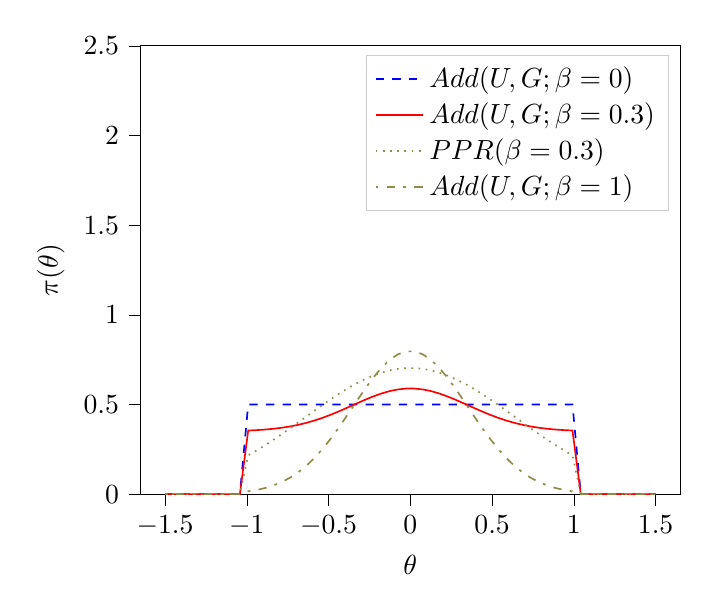
\begin{tikzpicture}

\begin{axis}[
legend cell align={left},
legend style={fill opacity=0.8, draw opacity=1, text opacity=1, draw=white!80!black},
tick align=outside,
tick pos=left,
x grid style={white!69.0196078431373!black},
xlabel={\(\displaystyle \theta\)},
xmin=-1.65, xmax=1.65,
xtick style={color=black},
y grid style={white!69.0196078431373!black},
ylabel={\(\displaystyle \pi(\theta)\)},
ymin=0, ymax=2.5,
ytick style={color=black}
]
\addplot [semithick, blue, dashed]
table {%
-1.5 0
-1.44915254237288 0
-1.39830508474576 0
-1.34745762711864 0
-1.29661016949153 0
-1.24576271186441 0
-1.19491525423729 0
-1.14406779661017 0
-1.09322033898305 0
-1.04237288135593 0
-0.991525423728814 0.5
-0.940677966101695 0.5
-0.889830508474576 0.5
-0.838983050847458 0.5
-0.788135593220339 0.5
-0.73728813559322 0.5
-0.686440677966102 0.5
-0.635593220338983 0.5
-0.584745762711864 0.5
-0.533898305084746 0.5
-0.483050847457627 0.5
-0.432203389830508 0.5
-0.38135593220339 0.5
-0.330508474576271 0.5
-0.279661016949152 0.5
-0.228813559322034 0.5
-0.177966101694915 0.5
-0.127118644067796 0.5
-0.0762711864406778 0.5
-0.0254237288135593 0.5
0.0254237288135595 0.5
0.076271186440678 0.5
0.127118644067797 0.5
0.177966101694915 0.5
0.228813559322034 0.5
0.279661016949153 0.5
0.330508474576271 0.5
0.38135593220339 0.5
0.432203389830509 0.5
0.483050847457627 0.5
0.533898305084746 0.5
0.584745762711865 0.5
0.635593220338983 0.5
0.686440677966102 0.5
0.737288135593221 0.5
0.788135593220339 0.5
0.838983050847458 0.5
0.889830508474577 0.5
0.940677966101695 0.5
0.991525423728814 0.5
1.04237288135593 0
1.09322033898305 0
1.14406779661017 0
1.19491525423729 0
1.24576271186441 0
1.29661016949153 0
1.34745762711864 0
1.39830508474576 0
1.44915254237288 0
1.5 0
};
\addlegendentry{$Add(U, G; \beta=0)$}
\addplot [semithick, red]
table {%
-1.5 0
-1.44915254237288 0
-1.39830508474576 0
-1.34745762711864 0
-1.29661016949153 0
-1.24576271186441 0
-1.19491525423729 0
-1.14406779661017 0
-1.09322033898305 0
-1.04237288135593 0
-0.991525423728814 0.354690318349014
-0.940677966101695 0.356948257984
-0.889830508474576 0.360082465104504
-0.838983050847458 0.364330940676924
-0.788135593220339 0.369952616124693
-0.73728813559322 0.377210854126332
-0.686440677966102 0.386349771016284
-0.635593220338983 0.397563999166328
-0.584745762711864 0.410963827347145
-0.533898305084746 0.426539084688447
-0.483050847457627 0.444126407270881
-0.432203389830508 0.463385332657938
-0.38135593220339 0.483788705911657
-0.330508474576271 0.504631940380111
-0.279661016949152 0.525063713430144
-0.228813559322034 0.54413786330865
-0.177966101694915 0.560882981292239
-0.127118644067796 0.574383024711279
-0.0762711864406778 0.583859836479305
-0.0254237288135593 0.588747297055759
0.0254237288135595 0.588747297055759
0.076271186440678 0.583859836479305
0.127118644067797 0.574383024711279
0.177966101694915 0.560882981292239
0.228813559322034 0.54413786330865
0.279661016949153 0.525063713430144
0.330508474576271 0.504631940380111
0.38135593220339 0.483788705911657
0.432203389830509 0.463385332657938
0.483050847457627 0.444126407270881
0.533898305084746 0.426539084688447
0.584745762711865 0.410963827347145
0.635593220338983 0.397563999166328
0.686440677966102 0.386349771016284
0.737288135593221 0.377210854126332
0.788135593220339 0.369952616124693
0.838983050847458 0.364330940676924
0.889830508474577 0.360082465104504
0.940677966101695 0.356948257984
0.991525423728814 0.354690318349014
1.04237288135593 0
1.09322033898305 0
1.14406779661017 0
1.19491525423729 0
1.24576271186441 0
1.29661016949153 0
1.34745762711864 0
1.39830508474576 0
1.44915254237288 0
1.5 0
};
\addlegendentry{$Add(U, G;\beta=0.3)$}
\addplot [semithick, yellow!50!black, dotted]
table {%
-1.5 0
-1.44915254237288 0
-1.39830508474576 0
-1.34745762711864 0
-1.29661016949153 0
-1.24576271186441 0
-1.19491525423729 0
-1.14406779661017 0
-1.09322033898305 0
-1.04237288135593 0
-0.991525423728814 0.216189593234766
-0.940677966101695 0.243241049554894
-0.889830508474576 0.27198446961261
-0.838983050847458 0.302243171403917
-0.788135593220339 0.333790553940582
-0.73728813559322 0.366350459314597
-0.686440677966102 0.399599183303834
-0.635593220338983 0.433169227869832
-0.584745762711864 0.466654819495022
-0.533898305084746 0.499619139927575
-0.483050847457627 0.531603134276833
-0.432203389830508 0.56213567986932
-0.38135593220339 0.59074482252954
-0.330508474576271 0.616969719742002
-0.279661016949152 0.640372876960198
-0.228813559322034 0.660552228031033
-0.177966101694915 0.677152596268245
-0.127118644067796 0.689876080941671
-0.0762711864406778 0.698490945314958
-0.0254237288135593 0.702838635897227
0.0254237288135595 0.702838635897227
0.076271186440678 0.698490945314958
0.127118644067797 0.689876080941671
0.177966101694915 0.677152596268245
0.228813559322034 0.660552228031033
0.279661016949153 0.640372876960198
0.330508474576271 0.616969719742002
0.38135593220339 0.59074482252954
0.432203389830509 0.56213567986932
0.483050847457627 0.531603134276833
0.533898305084746 0.499619139927575
0.584745762711865 0.466654819495021
0.635593220338983 0.433169227869832
0.686440677966102 0.399599183303834
0.737288135593221 0.366350459314597
0.788135593220339 0.333790553940582
0.838983050847458 0.302243171403917
0.889830508474577 0.27198446961261
0.940677966101695 0.243241049554894
0.991525423728814 0.216189593234766
1.04237288135593 0
1.09322033898305 0
1.14406779661017 0
1.19491525423729 0
1.24576271186441 0
1.29661016949153 0
1.34745762711864 0
1.39830508474576 0
1.44915254237288 0
1.5 0
};
\addlegendentry{$PPR(\beta=0.3)$}
\addplot [semithick, yellow!50!black, dash pattern=on 1pt off 3pt on 3pt off 3pt]
table {%
-1.5 0
-1.44915254237288 0
-1.39830508474576 0
-1.34745762711864 0
-1.29661016949153 0
-1.24576271186441 0
-1.19491525423729 0
-1.14406779661017 0
-1.09322033898305 0
-1.04237288135593 0
-0.991525423728814 0.015634394496712
-0.940677966101695 0.0231608599466659
-0.889830508474576 0.0336082170150122
-0.838983050847458 0.0477698022564135
-0.788135593220339 0.066508720415643
-0.73728813559322 0.0907028470877726
-0.686440677966102 0.121165903387615
-0.635593220338983 0.15854666388776
-0.584745762711864 0.203212757823817
-0.533898305084746 0.255130282294824
-0.483050847457627 0.313754690902936
-0.432203389830508 0.377951108859794
-0.38135593220339 0.445962353038858
-0.330508474576271 0.515439801267037
-0.279661016949152 0.583545711433813
-0.228813559322034 0.647126211028834
-0.177966101694915 0.702943270974129
-0.127118644067796 0.747943415704262
-0.0762711864406778 0.77953278826435
-0.0254237288135593 0.795824323519198
0.0254237288135595 0.795824323519198
0.076271186440678 0.77953278826435
0.127118644067797 0.747943415704262
0.177966101694915 0.702943270974129
0.228813559322034 0.647126211028834
0.279661016949153 0.583545711433812
0.330508474576271 0.515439801267037
0.38135593220339 0.445962353038858
0.432203389830509 0.377951108859794
0.483050847457627 0.313754690902936
0.533898305084746 0.255130282294824
0.584745762711865 0.203212757823817
0.635593220338983 0.15854666388776
0.686440677966102 0.121165903387615
0.737288135593221 0.0907028470877724
0.788135593220339 0.0665087204156429
0.838983050847458 0.0477698022564135
0.889830508474577 0.0336082170150121
0.940677966101695 0.0231608599466659
0.991525423728814 0.015634394496712
1.04237288135593 0
1.09322033898305 0
1.14406779661017 0
1.19491525423729 0
1.24576271186441 0
1.29661016949153 0
1.34745762711864 0
1.39830508474576 0
1.44915254237288 0
1.5 0
};
\addlegendentry{$Add(U, G; \beta=1)$}
\end{axis}

\end{tikzpicture}

  \caption{\label{fig:additive} An additive isometric mixture of a
    Gaussian iPPR and a uniform reference. PPR added for comparison.}
\end{figure}

Additive mixtures are an attempt to relax some of the limitations
imposed on PPR. Firstly, our proposals are limited to a class of
functions, defined by a power relation. Fortunately for PPR, this
class always includes a uniform prior, but not, for example a
``wedding cake'' prior (stepped uniform prior). This also means that
we are limited to only one intuitive proposal: we can't for example use
two non-concentric Gaussian peaks without extra
parametrisation\footnote{There is a more subtle point,
  \cref{obj-property} is violated because of the extreme bias towards
  the prior peak, that is present for every value of $\beta\ne0$. More
  on that later.}. While we do gain that freedom, it comes at a cost.

The downfall of additive mixtures lies in the definition of
$\tilde{\cal L}$. Instead of having to evaluate only one of the
constituent likelihoods, we are forced to evaluate all of them. This
means that we restrict time complexity to
\begin{equation}
  {\cal T}\{\tilde{\cal L}\} = O \left(   \max_{i} {\cal T}\{ {\cal L_{i}}\}. \right)\label{eq:hard-cap}
\end{equation}
This issue can be mitigated with asynchronous computation, provided
there is no interference. Another optimisation may be possible if the
likelihoods are related via an easy to compute correction.  This,
however requires low-level access to the implementation of nested
sampling.

Another issue is that the overall likelihood depends on the prior PDFs
of the constituents. To highlight why this is a problem, note that
nested sampling almost always requires the specification of prior via
its quantile. Function inversion is not linear with respect to
addition, so the quantile of the weighted sum needs to be evaluated
for each type of mixture individually. For a linear combination of
uniform priors, evaluating the quantile can be done elegantly, but not
in case of two Gaussians or a Gaussian mixed with a uniform. More
priors make this even more complicated.

These issues mostly stem from two sources: the likelihood depends in
general on all the values of its constituent likelihoods and
integration followed by inversion is not linear with respect to
addition.

In the following section we shall describe a mixing algorithm that
sidesteps both issues, by means of deterministic, stochastic
branching, that effectively creates a superposition of the priors,
rather than using any other mathematical operation.

\subsubsection{Stochastic superpositional isometric mixtures}

We want to superimpose consistent partitioning schemes $\pi_{i}$,
${\cal L}_{i}$, by adding \(m-1\) extra parameters $\bm{\beta}$. 
Firstly, the parameterised prior is 
\begin{equation}
  \tilde{\pi}(\bm{\theta}; \beta)  \triangleq
  \begin{cases}
	\tilde{\pi}_{1}(\bm{\theta}) & \text{with probability } \beta_{1},\\
	& \vdots,\\
	\tilde{\pi}_{n}(\bm{\theta}) & \text{with probability } (1- \sum_{i}^{m}\beta_{i}),
	\end{cases}
\end{equation}
and likelihood:
\begin{equation}
  \tilde{\cal L}(\bm{\theta}; \bm{\beta})  \triangleq
  \begin{cases}
	\tilde{\cal L}_{1}(\bm{\theta}) &  \text{with probability } \beta_{1},\\
		    &\vdots,\\
	\tilde{\cal L}_{m}(\bm{\theta}) & \text{with probability} (1- \sum_{i}^{m}\beta_{i}).
\end{cases}
\end{equation}
It is a consistent partitioning of the original model if and only if
\begin{equation}
  \label{eq:sspr}
  \tilde{\pi}(\bm{\theta}; \bm{\beta}) = \tilde{\pi}(\bm{\theta})_{i} \Leftrightarrow \tilde{\cal L}(\bm{\theta}; \bm{\beta}) = \tilde{\cal L}_{m}(\bm{\theta}; \bm{\beta}), 
\end{equation}
that is, the branches are chosen consistently.

The~\cref{spec-prop,norm-prop} are satisfied by construction if at
least one of the priors represented the
posterior. The~\cref{vconv-prop} is satisfied similarly to PPR: the
likelihood is determined by \(\bm\tilde{\theta} \sup \bm{\beta}\), so
$\bm{\beta}$s that lead to higher likelihoods are favoured, ergo
configurations where ${\cal P}$ is represented are also preferred.

Superpositional mixtures have multiple advantages when compared with
additive mixtures. Crucially, only one of ${\cal L}_{i}$ is evaluated
each time $\tilde{\cal L}$ is evaluated. As a result, ignoring the
overhead of branch choice, the worst case time complexity is better
than the best case for additive mixtures. This has vast implications
discussed in \cref{sec:applications}.

Moreover, superpositional mixtures branch choice is external to the
likelihoods and independent of them. Consequently, specifications of
$\pi_{i}$ via quantile are sufficient, and we do not need to perform
any other calculations.


There can be many implementations of a superpositional mixture. A
natural first choice would be a quantum computer, where the
$\tilde{\pi}$ and $\tilde{\cal L}$ are represented by \(m\) level
systems entangled with each other (consistent choice of branch) and a
classical computer (to evaluate ${\cal L}$ and $\pi$). However, we can
also attain an implementation using only computational methods via a
stochastic choice.

\emph{Stochastic superpositional isometric mixture} of consistent
partitioning (SSIM) ensures branch consistency by requiring
\begin{equation}
\tilde{\pi}(\bm{\theta}; \bm{\beta}) = \tilde{\pi}_{F(\bm{\theta};
  \bm{\beta})}(\bm{\theta};\bm{\beta}),
\end{equation}
where $F(\bm{\theta}; \bm{\beta})$ is a function. In our implementation
\begin{equation}
  F(\bm{\theta};\bm{\beta})= \text{{\cal N}}_{m}\left(\text{pseudo-random}(\bm{\theta}); \bm{\beta}\right)
\end{equation}
where \({\cal N}_{m}\) is the smallest index \(n \leq m\) for
which
\begin{equation}
x > \sum_{i}\beta_{i}.
\end{equation}
This implementation of SSIM is illustrated in \cref{fig:mixture}.

Domains of individual models are not a concern, provided we require
that if $\theta_{e} \not\in D(\pi_{i})$ then
${\cal L}_{i}(\theta_{e})=0$ for $i=1,\ldots,m$, contrary to what
\cref{norm-prop} may suggest. The effective domain of SSIM is the
set union of the domains of its constituents.

\begin{figure}  
  % This file was created by tikzplotlib v0.9.1.
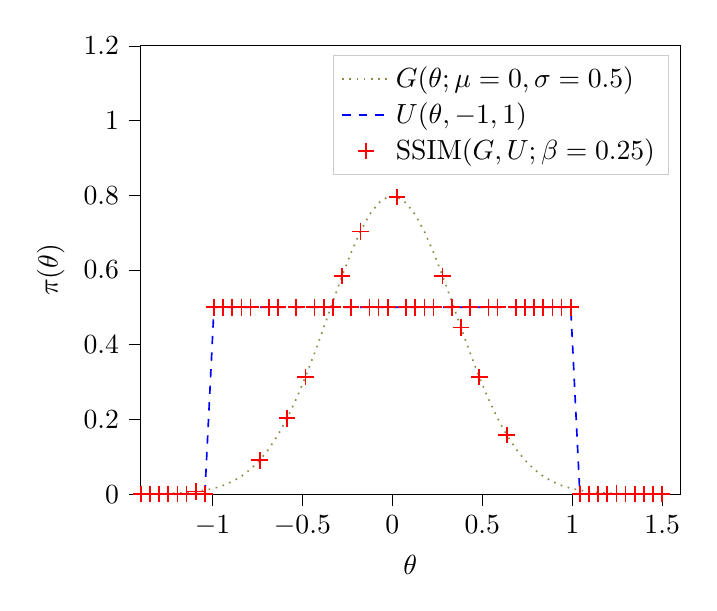
\begin{tikzpicture}

\begin{axis}[
legend cell align={left},
legend style={fill opacity=0.8, draw opacity=1, text opacity=1, draw=white!80!black},
tick align=outside,
tick pos=left,
x grid style={white!69.0196078431373!black},
xlabel={\(\displaystyle \theta\)},
xmin=-1.4, xmax=1.6,
xtick style={color=black},
y grid style={white!69.0196078431373!black},
ylabel={\(\displaystyle \pi(\theta)\)},
ymin=0, ymax=1.2,
ytick style={color=black}
]
\addplot [semithick, yellow!50!black, dotted]
table {%
-1.5 9.8466777332468e-05
-1.44915254237288 0.0001793872435764
-1.39830508474576 0.000320118348094559
-1.34745762711864 0.000559560121531124
-1.29661016949153 0.000958076356441112
-1.24576271186441 0.00160683272401611
-1.19491525423729 0.00263972321036136
-1.14406779661017 0.00424779248787262
-1.09322033898305 0.00669553635076534
-1.04237288135593 0.0103377167883577
-0.991525423728814 0.015634394496712
-0.940677966101695 0.0231608599466659
-0.889830508474576 0.0336082170150122
-0.838983050847458 0.0477698022564135
-0.788135593220339 0.066508720415643
-0.73728813559322 0.0907028470877726
-0.686440677966102 0.121165903387615
-0.635593220338983 0.15854666388776
-0.584745762711864 0.203212757823817
-0.533898305084746 0.255130282294824
-0.483050847457627 0.313754690902936
-0.432203389830508 0.377951108859794
-0.38135593220339 0.445962353038858
-0.330508474576271 0.515439801267037
-0.279661016949152 0.583545711433813
-0.228813559322034 0.647126211028834
-0.177966101694915 0.702943270974129
-0.127118644067796 0.747943415704262
-0.0762711864406778 0.77953278826435
-0.0254237288135593 0.795824323519198
0.0254237288135595 0.795824323519198
0.076271186440678 0.77953278826435
0.127118644067797 0.747943415704262
0.177966101694915 0.702943270974129
0.228813559322034 0.647126211028834
0.279661016949153 0.583545711433812
0.330508474576271 0.515439801267037
0.38135593220339 0.445962353038858
0.432203389830509 0.377951108859794
0.483050847457627 0.313754690902936
0.533898305084746 0.255130282294824
0.584745762711865 0.203212757823817
0.635593220338983 0.15854666388776
0.686440677966102 0.121165903387615
0.737288135593221 0.0907028470877724
0.788135593220339 0.0665087204156429
0.838983050847458 0.0477698022564135
0.889830508474577 0.0336082170150121
0.940677966101695 0.0231608599466659
0.991525423728814 0.015634394496712
1.04237288135593 0.0103377167883577
1.09322033898305 0.00669553635076532
1.14406779661017 0.00424779248787262
1.19491525423729 0.00263972321036135
1.24576271186441 0.0016068327240161
1.29661016949153 0.000958076356441112
1.34745762711864 0.000559560121531121
1.39830508474576 0.000320118348094558
1.44915254237288 0.000179387243576399
1.5 9.8466777332468e-05
};
\addlegendentry{$G(\theta; \mu=0, \sigma=0.5)$}
\addplot [semithick, blue, dashed]
table {%
-1.5 0
-1.44915254237288 0
-1.39830508474576 0
-1.34745762711864 0
-1.29661016949153 0
-1.24576271186441 0
-1.19491525423729 0
-1.14406779661017 0
-1.09322033898305 0
-1.04237288135593 0
-0.991525423728814 0.5
-0.940677966101695 0.5
-0.889830508474576 0.5
-0.838983050847458 0.5
-0.788135593220339 0.5
-0.73728813559322 0.5
-0.686440677966102 0.5
-0.635593220338983 0.5
-0.584745762711864 0.5
-0.533898305084746 0.5
-0.483050847457627 0.5
-0.432203389830508 0.5
-0.38135593220339 0.5
-0.330508474576271 0.5
-0.279661016949152 0.5
-0.228813559322034 0.5
-0.177966101694915 0.5
-0.127118644067796 0.5
-0.0762711864406778 0.5
-0.0254237288135593 0.5
0.0254237288135595 0.5
0.076271186440678 0.5
0.127118644067797 0.5
0.177966101694915 0.5
0.228813559322034 0.5
0.279661016949153 0.5
0.330508474576271 0.5
0.38135593220339 0.5
0.432203389830509 0.5
0.483050847457627 0.5
0.533898305084746 0.5
0.584745762711865 0.5
0.635593220338983 0.5
0.686440677966102 0.5
0.737288135593221 0.5
0.788135593220339 0.5
0.838983050847458 0.5
0.889830508474577 0.5
0.940677966101695 0.5
0.991525423728814 0.5
1.04237288135593 0
1.09322033898305 0
1.14406779661017 0
1.19491525423729 0
1.24576271186441 0
1.29661016949153 0
1.34745762711864 0
1.39830508474576 0
1.44915254237288 0
1.5 0
};
\addlegendentry{$U(\theta, -1, 1)$}
\addplot [semithick, red, mark=+, mark size=3, mark options={solid}, only marks]
table {%
-1.5 0
-1.44915254237288 0
-1.39830508474576 0
-1.34745762711864 0
-1.29661016949153 0
-1.24576271186441 0
-1.19491525423729 0
-1.14406779661017 0
-1.09322033898305 0.00669553635076534
-1.04237288135593 0
-0.991525423728814 0.5
-0.940677966101695 0.5
-0.889830508474576 0.5
-0.838983050847458 0.5
-0.788135593220339 0.5
-0.73728813559322 0.0907028470877726
-0.686440677966102 0.5
-0.635593220338983 0.5
-0.584745762711864 0.203212757823817
-0.533898305084746 0.5
-0.483050847457627 0.313754690902936
-0.432203389830508 0.5
-0.38135593220339 0.5
-0.330508474576271 0.5
-0.279661016949152 0.583545711433813
-0.228813559322034 0.5
-0.177966101694915 0.702943270974129
-0.127118644067796 0.5
-0.0762711864406778 0.5
-0.0254237288135593 0.5
0.0254237288135595 0.795824323519198
0.076271186440678 0.5
0.127118644067797 0.5
0.177966101694915 0.5
0.228813559322034 0.5
0.279661016949153 0.583545711433812
0.330508474576271 0.5
0.38135593220339 0.445962353038858
0.432203389830509 0.5
0.483050847457627 0.313754690902936
0.533898305084746 0.5
0.584745762711865 0.5
0.635593220338983 0.15854666388776
0.686440677966102 0.5
0.737288135593221 0.5
0.788135593220339 0.5
0.838983050847458 0.5
0.889830508474577 0.5
0.940677966101695 0.5
0.991525423728814 0.5
1.04237288135593 0
1.09322033898305 0
1.14406779661017 0
1.19491525423729 0
1.24576271186441 0.0016068327240161
1.29661016949153 0
1.34745762711864 0
1.39830508474576 0
1.44915254237288 0
1.5 0
};
\addlegendentry{SSIM$(G, U; \beta=0.25)$}
\end{axis}

\end{tikzpicture}


  % This file was created by tikzplotlib v0.9.1.
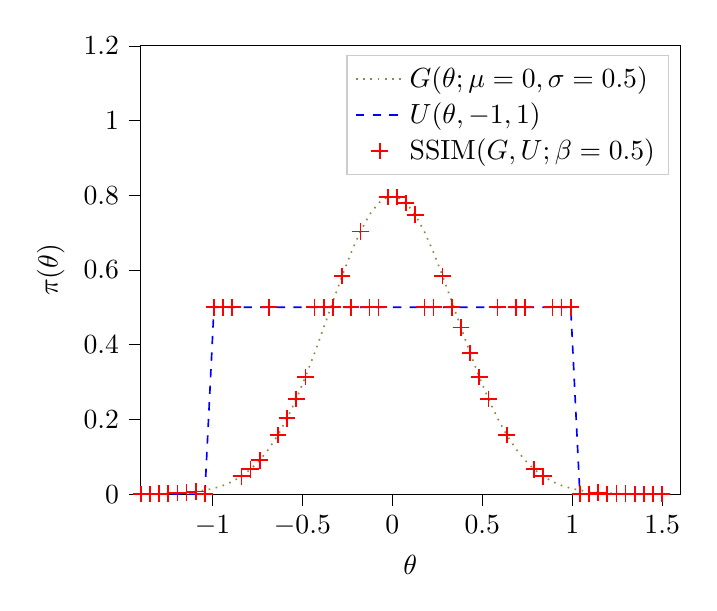
\begin{tikzpicture}

\begin{axis}[
legend cell align={left},
legend style={fill opacity=0.8, draw opacity=1, text opacity=1, draw=white!80!black},
tick align=outside,
tick pos=left,
x grid style={white!69.0196078431373!black},
xlabel={\(\displaystyle \theta\)},
xmin=-1.4, xmax=1.6,
xtick style={color=black},
y grid style={white!69.0196078431373!black},
ylabel={\(\displaystyle \pi(\theta)\)},
ymin=0, ymax=1.2,
ytick style={color=black}
]
\addplot [semithick, yellow!50!black, dotted]
table {%
-1.5 9.8466777332468e-05
-1.44915254237288 0.0001793872435764
-1.39830508474576 0.000320118348094559
-1.34745762711864 0.000559560121531124
-1.29661016949153 0.000958076356441112
-1.24576271186441 0.00160683272401611
-1.19491525423729 0.00263972321036136
-1.14406779661017 0.00424779248787262
-1.09322033898305 0.00669553635076534
-1.04237288135593 0.0103377167883577
-0.991525423728814 0.015634394496712
-0.940677966101695 0.0231608599466659
-0.889830508474576 0.0336082170150122
-0.838983050847458 0.0477698022564135
-0.788135593220339 0.066508720415643
-0.73728813559322 0.0907028470877726
-0.686440677966102 0.121165903387615
-0.635593220338983 0.15854666388776
-0.584745762711864 0.203212757823817
-0.533898305084746 0.255130282294824
-0.483050847457627 0.313754690902936
-0.432203389830508 0.377951108859794
-0.38135593220339 0.445962353038858
-0.330508474576271 0.515439801267037
-0.279661016949152 0.583545711433813
-0.228813559322034 0.647126211028834
-0.177966101694915 0.702943270974129
-0.127118644067796 0.747943415704262
-0.0762711864406778 0.77953278826435
-0.0254237288135593 0.795824323519198
0.0254237288135595 0.795824323519198
0.076271186440678 0.77953278826435
0.127118644067797 0.747943415704262
0.177966101694915 0.702943270974129
0.228813559322034 0.647126211028834
0.279661016949153 0.583545711433812
0.330508474576271 0.515439801267037
0.38135593220339 0.445962353038858
0.432203389830509 0.377951108859794
0.483050847457627 0.313754690902936
0.533898305084746 0.255130282294824
0.584745762711865 0.203212757823817
0.635593220338983 0.15854666388776
0.686440677966102 0.121165903387615
0.737288135593221 0.0907028470877724
0.788135593220339 0.0665087204156429
0.838983050847458 0.0477698022564135
0.889830508474577 0.0336082170150121
0.940677966101695 0.0231608599466659
0.991525423728814 0.015634394496712
1.04237288135593 0.0103377167883577
1.09322033898305 0.00669553635076532
1.14406779661017 0.00424779248787262
1.19491525423729 0.00263972321036135
1.24576271186441 0.0016068327240161
1.29661016949153 0.000958076356441112
1.34745762711864 0.000559560121531121
1.39830508474576 0.000320118348094558
1.44915254237288 0.000179387243576399
1.5 9.8466777332468e-05
};
\addlegendentry{$G(\theta; \mu=0, \sigma=0.5)$}
\addplot [semithick, blue, dashed]
table {%
-1.5 0
-1.44915254237288 0
-1.39830508474576 0
-1.34745762711864 0
-1.29661016949153 0
-1.24576271186441 0
-1.19491525423729 0
-1.14406779661017 0
-1.09322033898305 0
-1.04237288135593 0
-0.991525423728814 0.5
-0.940677966101695 0.5
-0.889830508474576 0.5
-0.838983050847458 0.5
-0.788135593220339 0.5
-0.73728813559322 0.5
-0.686440677966102 0.5
-0.635593220338983 0.5
-0.584745762711864 0.5
-0.533898305084746 0.5
-0.483050847457627 0.5
-0.432203389830508 0.5
-0.38135593220339 0.5
-0.330508474576271 0.5
-0.279661016949152 0.5
-0.228813559322034 0.5
-0.177966101694915 0.5
-0.127118644067796 0.5
-0.0762711864406778 0.5
-0.0254237288135593 0.5
0.0254237288135595 0.5
0.076271186440678 0.5
0.127118644067797 0.5
0.177966101694915 0.5
0.228813559322034 0.5
0.279661016949153 0.5
0.330508474576271 0.5
0.38135593220339 0.5
0.432203389830509 0.5
0.483050847457627 0.5
0.533898305084746 0.5
0.584745762711865 0.5
0.635593220338983 0.5
0.686440677966102 0.5
0.737288135593221 0.5
0.788135593220339 0.5
0.838983050847458 0.5
0.889830508474577 0.5
0.940677966101695 0.5
0.991525423728814 0.5
1.04237288135593 0
1.09322033898305 0
1.14406779661017 0
1.19491525423729 0
1.24576271186441 0
1.29661016949153 0
1.34745762711864 0
1.39830508474576 0
1.44915254237288 0
1.5 0
};
\addlegendentry{$U(\theta, -1, 1)$}
\addplot [semithick, red, mark=+, mark size=3, mark options={solid}, only marks]
table {%
-1.5 9.8466777332468e-05
-1.44915254237288 0.0001793872435764
-1.39830508474576 0
-1.34745762711864 0.000559560121531124
-1.29661016949153 0.000958076356441112
-1.24576271186441 0.00160683272401611
-1.19491525423729 0.00263972321036136
-1.14406779661017 0.00424779248787262
-1.09322033898305 0.00669553635076534
-1.04237288135593 0
-0.991525423728814 0.5
-0.940677966101695 0.5
-0.889830508474576 0.5
-0.838983050847458 0.0477698022564135
-0.788135593220339 0.066508720415643
-0.73728813559322 0.0907028470877726
-0.686440677966102 0.5
-0.635593220338983 0.15854666388776
-0.584745762711864 0.203212757823817
-0.533898305084746 0.255130282294824
-0.483050847457627 0.313754690902936
-0.432203389830508 0.5
-0.38135593220339 0.5
-0.330508474576271 0.5
-0.279661016949152 0.583545711433813
-0.228813559322034 0.5
-0.177966101694915 0.702943270974129
-0.127118644067796 0.5
-0.0762711864406778 0.5
-0.0254237288135593 0.795824323519198
0.0254237288135595 0.795824323519198
0.076271186440678 0.77953278826435
0.127118644067797 0.747943415704262
0.177966101694915 0.5
0.228813559322034 0.5
0.279661016949153 0.583545711433812
0.330508474576271 0.5
0.38135593220339 0.445962353038858
0.432203389830509 0.377951108859794
0.483050847457627 0.313754690902936
0.533898305084746 0.255130282294824
0.584745762711865 0.5
0.635593220338983 0.15854666388776
0.686440677966102 0.5
0.737288135593221 0.5
0.788135593220339 0.0665087204156429
0.838983050847458 0.0477698022564135
0.889830508474577 0.5
0.940677966101695 0.5
0.991525423728814 0.5
1.04237288135593 0
1.09322033898305 0
1.14406779661017 0.00424779248787262
1.19491525423729 0
1.24576271186441 0.0016068327240161
1.29661016949153 0.000958076356441112
1.34745762711864 0
1.39830508474576 0.000320118348094558
1.44915254237288 0
1.5 9.8466777332468e-05
};
\addlegendentry{SSIM$(G, U; \beta=0.5)$}
\end{axis}

\end{tikzpicture}


  % This file was created by tikzplotlib v0.9.1.
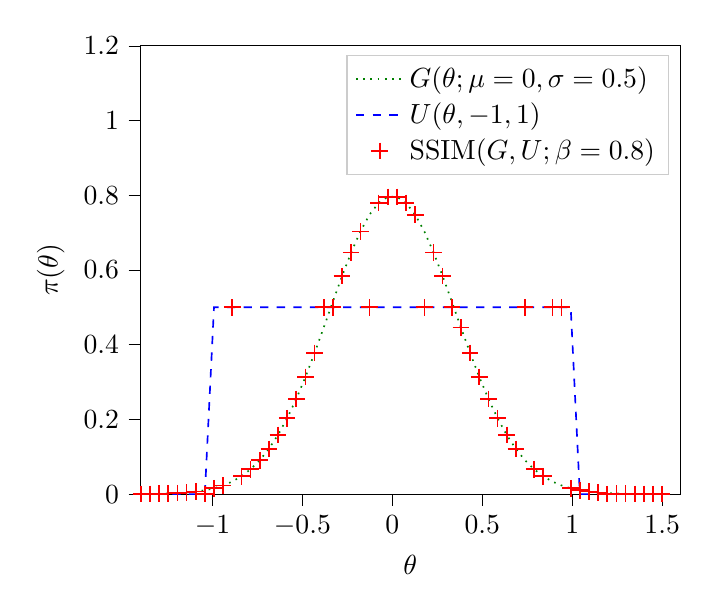
\begin{tikzpicture}

\begin{axis}[
legend cell align={left},
legend style={fill opacity=0.8, draw opacity=1, text opacity=1, draw=white!80!black},
tick align=outside,
tick pos=left,
x grid style={white!69.0196078431373!black},
xlabel={\(\displaystyle \theta\)},
xmin=-1.4, xmax=1.6,
xtick style={color=black},
y grid style={white!69.0196078431373!black},
ylabel={\(\displaystyle \pi(\theta)\)},
ymin=0, ymax=1.2,
ytick style={color=black}
]
\addplot [semithick, green!50!black, dotted]
table {%
-1.5 9.8466777332468e-05
-1.44915254237288 0.0001793872435764
-1.39830508474576 0.000320118348094559
-1.34745762711864 0.000559560121531124
-1.29661016949153 0.000958076356441112
-1.24576271186441 0.00160683272401611
-1.19491525423729 0.00263972321036136
-1.14406779661017 0.00424779248787262
-1.09322033898305 0.00669553635076534
-1.04237288135593 0.0103377167883577
-0.991525423728814 0.015634394496712
-0.940677966101695 0.0231608599466659
-0.889830508474576 0.0336082170150122
-0.838983050847458 0.0477698022564135
-0.788135593220339 0.066508720415643
-0.73728813559322 0.0907028470877726
-0.686440677966102 0.121165903387615
-0.635593220338983 0.15854666388776
-0.584745762711864 0.203212757823817
-0.533898305084746 0.255130282294824
-0.483050847457627 0.313754690902936
-0.432203389830508 0.377951108859794
-0.38135593220339 0.445962353038858
-0.330508474576271 0.515439801267037
-0.279661016949152 0.583545711433813
-0.228813559322034 0.647126211028834
-0.177966101694915 0.702943270974129
-0.127118644067796 0.747943415704262
-0.0762711864406778 0.77953278826435
-0.0254237288135593 0.795824323519198
0.0254237288135595 0.795824323519198
0.076271186440678 0.77953278826435
0.127118644067797 0.747943415704262
0.177966101694915 0.702943270974129
0.228813559322034 0.647126211028834
0.279661016949153 0.583545711433812
0.330508474576271 0.515439801267037
0.38135593220339 0.445962353038858
0.432203389830509 0.377951108859794
0.483050847457627 0.313754690902936
0.533898305084746 0.255130282294824
0.584745762711865 0.203212757823817
0.635593220338983 0.15854666388776
0.686440677966102 0.121165903387615
0.737288135593221 0.0907028470877724
0.788135593220339 0.0665087204156429
0.838983050847458 0.0477698022564135
0.889830508474577 0.0336082170150121
0.940677966101695 0.0231608599466659
0.991525423728814 0.015634394496712
1.04237288135593 0.0103377167883577
1.09322033898305 0.00669553635076532
1.14406779661017 0.00424779248787262
1.19491525423729 0.00263972321036135
1.24576271186441 0.0016068327240161
1.29661016949153 0.000958076356441112
1.34745762711864 0.000559560121531121
1.39830508474576 0.000320118348094558
1.44915254237288 0.000179387243576399
1.5 9.8466777332468e-05
};
\addlegendentry{$G(\theta; \mu=0, \sigma=0.5)$}
\addplot [semithick, blue, dashed]
table {%
-1.5 0
-1.44915254237288 0
-1.39830508474576 0
-1.34745762711864 0
-1.29661016949153 0
-1.24576271186441 0
-1.19491525423729 0
-1.14406779661017 0
-1.09322033898305 0
-1.04237288135593 0
-0.991525423728814 0.5
-0.940677966101695 0.5
-0.889830508474576 0.5
-0.838983050847458 0.5
-0.788135593220339 0.5
-0.73728813559322 0.5
-0.686440677966102 0.5
-0.635593220338983 0.5
-0.584745762711864 0.5
-0.533898305084746 0.5
-0.483050847457627 0.5
-0.432203389830508 0.5
-0.38135593220339 0.5
-0.330508474576271 0.5
-0.279661016949152 0.5
-0.228813559322034 0.5
-0.177966101694915 0.5
-0.127118644067796 0.5
-0.0762711864406778 0.5
-0.0254237288135593 0.5
0.0254237288135595 0.5
0.076271186440678 0.5
0.127118644067797 0.5
0.177966101694915 0.5
0.228813559322034 0.5
0.279661016949153 0.5
0.330508474576271 0.5
0.38135593220339 0.5
0.432203389830509 0.5
0.483050847457627 0.5
0.533898305084746 0.5
0.584745762711865 0.5
0.635593220338983 0.5
0.686440677966102 0.5
0.737288135593221 0.5
0.788135593220339 0.5
0.838983050847458 0.5
0.889830508474577 0.5
0.940677966101695 0.5
0.991525423728814 0.5
1.04237288135593 0
1.09322033898305 0
1.14406779661017 0
1.19491525423729 0
1.24576271186441 0
1.29661016949153 0
1.34745762711864 0
1.39830508474576 0
1.44915254237288 0
1.5 0
};
\addlegendentry{$U(\theta, -1, 1)$}
\addplot [semithick, red, mark=+, mark size=3, mark options={solid}, only marks]
table {%
-1.5 9.8466777332468e-05
-1.44915254237288 0.0001793872435764
-1.39830508474576 0
-1.34745762711864 0.000559560121531124
-1.29661016949153 0.000958076356441112
-1.24576271186441 0.00160683272401611
-1.19491525423729 0.00263972321036136
-1.14406779661017 0.00424779248787262
-1.09322033898305 0.00669553635076534
-1.04237288135593 0
-0.991525423728814 0.015634394496712
-0.940677966101695 0.0231608599466659
-0.889830508474576 0.5
-0.838983050847458 0.0477698022564135
-0.788135593220339 0.066508720415643
-0.73728813559322 0.0907028470877726
-0.686440677966102 0.121165903387615
-0.635593220338983 0.15854666388776
-0.584745762711864 0.203212757823817
-0.533898305084746 0.255130282294824
-0.483050847457627 0.313754690902936
-0.432203389830508 0.377951108859794
-0.38135593220339 0.5
-0.330508474576271 0.5
-0.279661016949152 0.583545711433813
-0.228813559322034 0.647126211028834
-0.177966101694915 0.702943270974129
-0.127118644067796 0.5
-0.0762711864406778 0.77953278826435
-0.0254237288135593 0.795824323519198
0.0254237288135595 0.795824323519198
0.076271186440678 0.77953278826435
0.127118644067797 0.747943415704262
0.177966101694915 0.5
0.228813559322034 0.647126211028834
0.279661016949153 0.583545711433812
0.330508474576271 0.5
0.38135593220339 0.445962353038858
0.432203389830509 0.377951108859794
0.483050847457627 0.313754690902936
0.533898305084746 0.255130282294824
0.584745762711865 0.203212757823817
0.635593220338983 0.15854666388776
0.686440677966102 0.121165903387615
0.737288135593221 0.5
0.788135593220339 0.0665087204156429
0.838983050847458 0.0477698022564135
0.889830508474577 0.5
0.940677966101695 0.5
0.991525423728814 0.015634394496712
1.04237288135593 0.0103377167883577
1.09322033898305 0.00669553635076532
1.14406779661017 0.00424779248787262
1.19491525423729 0
1.24576271186441 0.0016068327240161
1.29661016949153 0.000958076356441112
1.34745762711864 0.000559560121531121
1.39830508474576 0.000320118348094558
1.44915254237288 0.000179387243576399
1.5 9.8466777332468e-05
};
\addlegendentry{SSIM$(G, U; \beta=0.8)$}
\end{axis}

\end{tikzpicture}

  \caption{An example of mixture repartitioning. The mixture is not
    normalised to emphasise the coincidence of values with both the
    uniform distribution and a Gaussian. $\beta$ controls the
    probability of belonging to the Gaussian in the stochastic
    mixture.  \label{fig:mixture}}
\end{figure}

SSIM, by fixing many of the issues of additive mixtures, inherits most
of the advantages. It is also much more robust, which we shall discuss
in the later sections. It does however come with one drawback. As a
result of branching, the likelihood '$\tilde{\cal L}$ visible to the
sampler, is no longer continuous. Thus nested sampling that relied on
said continuity will have undefined behaviour. \texttt{PolyChord}'s
slice sampling seems not affected by the discontinuity, but there may be
other samplers that are.
\section{Measurements and methodology}
We shall adopt the weighted accounting approach \citep{Cormen}, common
in computer science for measuring time complexity. Measuring time
complexity in units of \({\cal N}\{{\cal L}\}\), we shall reduce all
quantities to their long run averages. As a result, all of the
repartitioning schemes' overheads associated with internal
implementation details are ignored. As such additive mixtures are put
at an inherent disadvantage, because in the average case,
\begin{equation}
  \label{eq:additive-t-complexity}
  {\cal N}\{ \tilde{\cal L}\} = \sum_{i}^{m} {\cal N}\{{\cal L}_{i}\}. 
\end{equation}

An important quantity for measuring both the correctness of our result
and its performance is the Kullback-Leilber divergence
\citep{Kullback_1951}. For probability distributions
\(f(\bm{\theta})\) and \(g(\bm{\theta})\), it is defined as:
\begin{equation}
  \label{eq:kl-def}
  {\cal D}\{f, g \} = \int_{\Psi}f(\bm{\theta}) \ln \frac{f(\bm{\theta})}{g(\bm{\theta})} d \bm{\theta}.
\end{equation}
It is a pre-metric on the space of probability distributions: it is
not symmetric, it does not satisfy the triangle inequality (hence not
a full metric), but it being zero is equivalent to the distributions
being identical.

We use it in two contexts. Firstly, ${\cal D}\{\pi, {\cal P}\}$ is a
measure of how much information extracted from the posterior came from
the prior. The smaller the ${\cal D}$, the more informative our
prior. \Cref{fig:kl-scaling} clearly shows, that it is also a reliable
predictor of performance. In \cref{fig:kl-d}, we see that the amount
of information extracted from PPR, with growing offset also
increases. However, it does so sub-linearly, which combined with
\cref{fig:convergence}, makes the validity of the obtained posteriors
from PPR and SSIM, suspect. 

While a full point-wise residual analysis of the marginalised
posterior would have been much more in the spirit of Bayesian
statistics, in the interest of convenience, we use
${\cal D}\{ {\cal P}, \bar{\cal P}$ to quantify the correctness of the
obtained posterior, where $\bar{\cal P}$ is the posterior obtained
using a $\pi(\bm{\theta}) = \text{Const}$. 

However, most often when performing Bayesian inference, there is not
reference uniform or analytical result to compute ${\cal D}$ from. Our
last indicator of correctness is ${\cal Z}$ --- evidence. If the
evidence is incorrect, it indicates one of two possible errors. If it
is greater than the expected value, this indicates that
$\tilde{\cal L}$ was normalised incorrectly (\cref{fig:hist}). If it
is less than expected, it indicates that the intuitive proposal used in
the repartitioning is incorrect (\cref{fig:drift})\footnote{both
  follow from \cref{eq:bayes}, and under the assumption that the
  intuitive proposal was more informative than the original prior. }.


\begin{table}
  \centering
  
  \caption{Typical values of posterior-to-reference-posterior
    Kullback-Leibler divergence ${\cal D}\{{\cal P}, \bar{\cal P}\}$
    for the runs shown in \cref{fig:hist}. The inconsistent
    re-sizeable uniform had not been given an improper normalisation
    of $\tilde{\cal L} = {\cal L}$. It is of type \emph{Re-sizeable
      uniform} described in \cref{sec:resizeable}.}
  \begin{tabular}{lr}
    \textbf{Scheme} & ${\cal D}\{ {\cal P}, \bar{\cal P}\}$\\
    \hline
    Uniform & 0.000\\
    Analytical & 0.000\\
    $R$ & 0.724\\
    $PPR$ & 0.011\\
    $SSIM(U, G, R)$ & 0.007\\
  \end{tabular}
  \label{tab:hist}
\end{table}




\begin{figure}
  % This file was created by tikzplotlib v0.9.1.
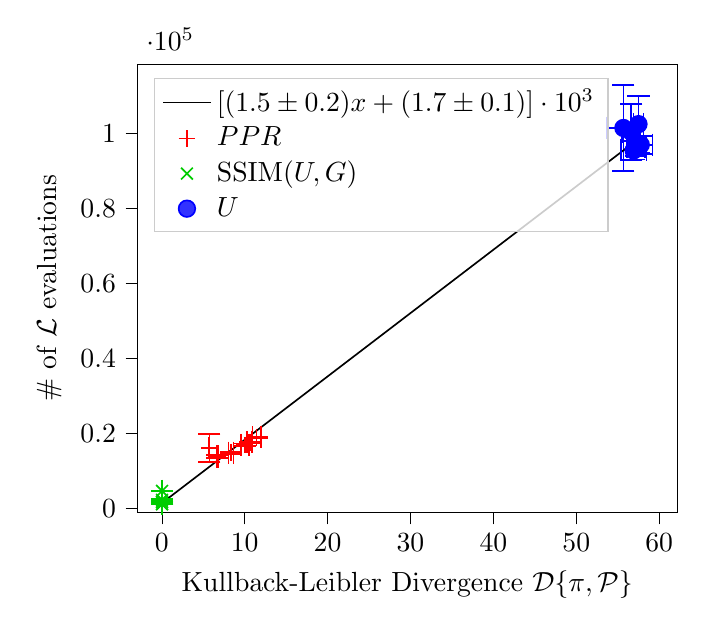
\begin{tikzpicture}

\definecolor{color0}{rgb}{1,0.0,0.0}
\definecolor{color1}{rgb}{0,0.8,0.0}
\definecolor{color2}{rgb}{0.0,0.0,1}
\definecolor{color3}{rgb}{0.0,0.0,0.0}

\begin{axis}[
legend cell align={left},
legend style={fill opacity=0.8, draw opacity=1, text opacity=1, at={(0.03,0.97)}, anchor=north west, draw=white!80!black},
tick align=outside,
tick pos=left,
x grid style={white!69.0196078431373!black},
xlabel={Kullback-Leibler Divergence \(\displaystyle {\cal D} \{\pi, {\cal P}\}\)},
xmin=-2.93567696145677, xmax=62.1613818701095,
xtick style={color=black},
y grid style={white!69.0196078431373!black},
ylabel={\# of \({\cal L}\) evaluations},
ymin=-1000.00, ymax=118545.85,
ytick style={color=black}
% ymode=log
]
\path [draw=color0, semithick]
(axis cs:5.71795365099151,16157.5)
--(axis cs:5.77133948534581,16157.5);

\path [draw=color0, semithick]
(axis cs:6.6768824419002,13953)
--(axis cs:6.77321107556694,13953);

\path [draw=color0, semithick]
(axis cs:8.02877279045042,14940.5)
--(axis cs:8.63543918622054,14940.5);

\path [draw=color0, semithick]
(axis cs:9.52185212376919,17043)
--(axis cs:10.4908349952443,17043);

\path [draw=color0, semithick]
(axis cs:10.3029683750536,17720.5)
--(axis cs:10.9155451202318,17720.5);

\path [draw=color0, semithick]
(axis cs:10.954510866509,19064.5)
--(axis cs:11.9335782130671,19064.5);

\path [draw=color0, semithick]
(axis cs:5.74464656816866,12446)
--(axis cs:5.74464656816866,19869);

\path [draw=color0, semithick]
(axis cs:6.72504675873357,13488)
--(axis cs:6.72504675873357,14418);

\path [draw=color0, semithick]
(axis cs:8.33210598833548,14689)
--(axis cs:8.33210598833548,15192);

\path [draw=color0, semithick]
(axis cs:10.0063435595067,16676)
--(axis cs:10.0063435595067,17410);

\path [draw=color0, semithick]
(axis cs:10.6092567476427,17618)
--(axis cs:10.6092567476427,17823);

\path [draw=color0, semithick]
(axis cs:11.4440445397881,18822)
--(axis cs:11.4440445397881,19307);

\path [draw=color1, semithick]
(axis cs:0.0271909650803472,2382.5)
--(axis cs:0.030089733601838,2382.5);

\path [draw=color1, semithick]
(axis cs:0.029683008672791,1207.5)
--(axis cs:0.0308036500189849,1207.5);

\path [draw=color1, semithick]
(axis cs:0.0282101242046804,1738.5)
--(axis cs:0.0298855157628486,1738.5);

\path [draw=color1, semithick]
(axis cs:0.0278177027329167,4757)
--(axis cs:0.0348526563256524,4757);

\path [draw=color1, semithick]
(axis cs:0.0232802581598788,1829.5)
--(axis cs:0.0301604324600733,1829.5);

\path [draw=color1, semithick]
(axis cs:0.0304771056975755,1224)
--(axis cs:0.0323746358923458,1224);

\path [draw=color1, semithick]
(axis cs:0.0286403493410926,2120)
--(axis cs:0.0286403493410926,2645);

\path [draw=color1, semithick]
(axis cs:0.0302433293458879,1163)
--(axis cs:0.0302433293458879,1252);

\path [draw=color1, semithick]
(axis cs:0.0290478199837645,1565)
--(axis cs:0.0290478199837645,1912);

\path [draw=color1, semithick]
(axis cs:0.0313351795292845,4698)
--(axis cs:0.0313351795292845,4816);

\path [draw=color1, semithick]
(axis cs:0.026720345309976,1740)
--(axis cs:0.026720345309976,1919);

\path [draw=color1, semithick]
(axis cs:0.0314258707949607,1138)
--(axis cs:0.0314258707949607,1310);

\path [draw=color2, semithick]
(axis cs:53.6407046096139,101541)
--(axis cs:57.7293889288474,101541);

\path [draw=color2, semithick]
(axis cs:56.1280894679801,96497)
--(axis cs:58.3022565457241,96497);

\path [draw=color2, semithick]
(axis cs:55.3633380690649,95565)
--(axis cs:58.47445725549,95565);

\path [draw=color2, semithick]
(axis cs:55.5223746731559,100523.5)
--(axis cs:57.7271641567295,100523.5);

\path [draw=color2, semithick]
(axis cs:56.8924880373743,102562.5)
--(axis cs:58.1261131182599,102562.5);

\path [draw=color2, semithick]
(axis cs:56.3603430284318,97066.5)
--(axis cs:59.2024246504929,97066.5);

\path [draw=color2, semithick]
(axis cs:55.6850467692306,90127)
--(axis cs:55.6850467692306,112955);

\path [draw=color2, semithick]
(axis cs:57.2151730068521,94020)
--(axis cs:57.2151730068521,98974);

\path [draw=color2, semithick]
(axis cs:56.9188976622774,93149)
--(axis cs:56.9188976622774,97981);

\path [draw=color2, semithick]
(axis cs:56.6247694149427,93079)
--(axis cs:56.6247694149427,107968);

\path [draw=color2, semithick]
(axis cs:57.5093005778171,94974)
--(axis cs:57.5093005778171,110151);

\path [draw=color2, semithick]
(axis cs:57.7813838394624,94657)
--(axis cs:57.7813838394624,99476);

\addplot [semithick, color0, mark=|, mark size=4, mark options={solid}, only marks, forget plot]
table {%
5.71795365099151 16157.5
6.6768824419002 13953
8.02877279045042 14940.5
9.52185212376919 17043
10.3029683750536 17720.5
10.954510866509 19064.5
};
\addplot [semithick, color0, mark=|, mark size=4, mark options={solid}, only marks, forget plot]
table {%
5.77133948534581 16157.5
6.77321107556694 13953
8.63543918622054 14940.5
10.4908349952443 17043
10.9155451202318 17720.5
11.9335782130671 19064.5
};
\addplot [semithick, color0, mark=-, mark size=4, mark options={solid}, only marks, forget plot]
table {%
5.74464656816866 12446
6.72504675873357 13488
8.33210598833548 14689
10.0063435595067 16676
10.6092567476427 17618
11.4440445397881 18822
};
\addplot [semithick, color0, mark=-, mark size=4, mark options={solid}, only marks, forget plot]
table {%
5.74464656816866 19869
6.72504675873357 14418
8.33210598833548 15192
10.0063435595067 17410
10.6092567476427 17823
11.4440445397881 19307
};
\addplot [semithick, color1, mark=|, mark size=4, mark options={solid}, only marks, forget plot]
table {%
0.0271909650803472 2382.5
0.029683008672791 1207.5
0.0282101242046804 1738.5
0.0278177027329167 4757
0.0232802581598788 1829.5
0.0304771056975755 1224
};
\addplot [semithick, color1, mark=|, mark size=4, mark options={solid}, only marks, forget plot]
table {%
0.030089733601838 2382.5
0.0308036500189849 1207.5
0.0298855157628486 1738.5
0.0348526563256524 4757
0.0301604324600733 1829.5
0.0323746358923458 1224
};
\addplot [semithick, color1, mark=-, mark size=4, mark options={solid}, only marks, forget plot]
table {%
0.0286403493410926 2120
0.0302433293458879 1163
0.0290478199837645 1565
0.0313351795292845 4698
0.026720345309976 1740
0.0314258707949607 1138
};
\addplot [semithick, color1, mark=-, mark size=4, mark options={solid}, only marks, forget plot]
table {%
0.0286403493410926 2645
0.0302433293458879 1252
0.0290478199837645 1912
0.0313351795292845 4816
0.026720345309976 1919
0.0314258707949607 1310
};
\addplot [semithick, color2, mark=|, mark size=4, mark options={solid}, only marks, forget plot]
table {%
53.6407046096139 101541
56.1280894679801 96497
55.3633380690649 95565
55.5223746731559 100523.5
56.8924880373743 102562.5
56.3603430284318 97066.5
};
\addplot [semithick, color2, mark=|, mark size=4, mark options={solid}, only marks, forget plot]
table {%
57.7293889288474 101541
58.3022565457241 96497
58.47445725549 95565
57.7271641567295 100523.5
58.1261131182599 102562.5
59.2024246504929 97066.5
};
\addplot [semithick, color2, mark=-, mark size=4, mark options={solid}, only marks, forget plot]
table {%
55.6850467692306 90127
57.2151730068521 94020
56.9188976622774 93149
56.6247694149427 93079
57.5093005778171 94974
57.7813838394624 94657
};
\addplot [semithick, color2, mark=-, mark size=4, mark options={solid}, only marks, forget plot]
table {%
55.6850467692306 112955
57.2151730068521 98974
56.9188976622774 97981
56.6247694149427 107968
57.5093005778171 110151
57.7813838394624 99476
};
\addplot [semithick, color3]
table {%
0.026720345309976 1539.88164299791
0.610100784644849 2525.39064984014
1.19348122397972 3510.89965668237
1.77686166331459 4496.4086635246
2.36024210264947 5481.91767036683
2.94362254198434 6467.42667720906
3.52700298131921 7452.93568405129
4.11038342065408 8438.44469089352
4.69376385998896 9423.95369773575
5.27714429932383 10409.462704578
5.8605247386587 11394.9717114202
6.44390517799357 12380.4807182624
7.02728561732845 13365.9897251047
7.61066605666332 14351.4987319469
8.19404649599819 15337.0077387891
8.77742693533306 16322.5167456314
9.36080737466794 17308.0257524736
9.94418781400281 18293.5347593158
10.5275682533377 19279.043766158
11.1109486926726 20264.5527730003
11.6943291320074 21250.0617798425
12.2777095713423 22235.5707866847
12.8610900106772 23221.079793527
13.444470450012 24206.5888003692
14.0278508893469 25192.0978072114
14.6112313286818 26177.6068140537
15.1946117680167 27163.1158208959
15.7779922073515 28148.6248277381
16.3613726466864 29134.1338345803
16.9447530860213 30119.6428414226
17.5281335253562 31105.1518482648
18.111513964691 32090.660855107
18.6948944040259 33076.1698619493
19.2782748433608 34061.6788687915
19.8616552826956 35047.1878756337
20.4450357220305 36032.6968824759
21.0284161613654 37018.2058893182
21.6117966007003 38003.7148961604
22.1951770400351 38989.2239030026
22.77855747937 39974.7329098449
23.3619379187049 40960.2419166871
23.9453183580397 41945.7509235293
24.5286987973746 42931.2599303716
25.1120792367095 43916.7689372138
25.6954596760444 44902.277944056
26.2788401153792 45887.7869508982
26.8622205547141 46873.2959577405
27.445600994049 47858.8049645827
28.0289814333839 48844.3139714249
28.6123618727187 49829.8229782672
29.1957423120536 50815.3319851094
29.7791227513885 51800.8409919516
30.3625031907233 52786.3499987938
30.9458836300582 53771.8590056361
31.5292640693931 54757.3680124783
32.112644508728 55742.8770193205
32.6960249480628 56728.3860261628
33.2794053873977 57713.895033005
33.8627858267326 58699.4040398472
34.4461662660675 59684.9130466895
35.0295467054023 60670.4220535317
35.6129271447372 61655.9310603739
36.1963075840721 62641.4400672161
36.7796880234069 63626.9490740584
37.3630684627418 64612.4580809006
37.9464489020767 65597.9670877428
38.5298293414116 66583.4760945851
39.1132097807464 67568.9851014273
39.6965902200813 68554.4941082695
40.2799706594162 69540.0031151118
40.863351098751 70525.512121954
41.4467315380859 71511.0211287962
42.0301119774208 72496.5301356384
42.6134924167557 73482.0391424807
43.1968728560905 74467.5481493229
43.7802532954254 75453.0571561651
44.3636337347603 76438.5661630074
44.9470141740952 77424.0751698496
45.53039461343 78409.5841766918
46.1137750527649 79395.093183534
46.6971554920998 80380.6021903763
47.2805359314346 81366.1111972185
47.8639163707695 82351.6202040607
48.4472968101044 83337.129210903
49.0306772494393 84322.6382177452
49.6140576887741 85308.1472245874
50.197438128109 86293.6562314297
50.7808185674439 87279.1652382719
51.3641990067788 88264.6742451141
51.9475794461136 89250.1832519564
52.5309598854485 90235.6922587986
53.1143403247834 91221.2012656408
53.6977207641182 92206.710272483
54.2811012034531 93192.2192793253
54.864481642788 94177.7282861675
55.4478620821229 95163.2372930097
56.0312425214577 96148.746299852
56.6146229607926 97134.2553066942
57.1980034001275 98119.7643135364
57.7813838394624 99105.2733203786
};
\addlegendentry{\(\left[(1.5 \pm 0.2)x + (1.7 \pm 0.1)\right]\cdot  10^3 \)}
\addplot [semithick, color0, mark=+, mark size=3, mark options={solid}, only marks]
table {%
5.74464656816866 16157.5
6.72504675873357 13953
8.33210598833548 14940.5
10.0063435595067 17043
10.6092567476427 17720.5
11.4440445397881 19064.5
};
\addlegendentry{$PPR$}
\addplot [semithick, color1, mark=x, mark size=3, mark options={solid}, only marks]
table {%
0.0286403493410926 2382.5
0.0302433293458879 1207.5
0.0290478199837645 1738.5
0.0313351795292845 4757
0.026720345309976 1829.5
0.0314258707949607 1224
};
\addlegendentry{SSIM$(U,G)$}
\addplot [semithick, color2, mark=*, mark size=3, mark options={solid}, only marks]
table {%
55.6850467692306 101541
57.2151730068521 96497
56.9188976622774 95565
56.6247694149427 100523.5
57.5093005778171 102562.5
57.7813838394624 97066.5
};
\addlegendentry{$U$}
\end{axis}

\end{tikzpicture}

\caption{Scaling of number of likelihood calls as a function of Kullback-Leibler divergence \({\cal D}\). The best fit line indicates that \({\cal D}\) is a reliable performance indicator for \texttt{PolyChord}.\label{fig:kl-scaling}}
\end{figure}


\begin{figure}
% This file was created by tikzplotlib v0.9.1.
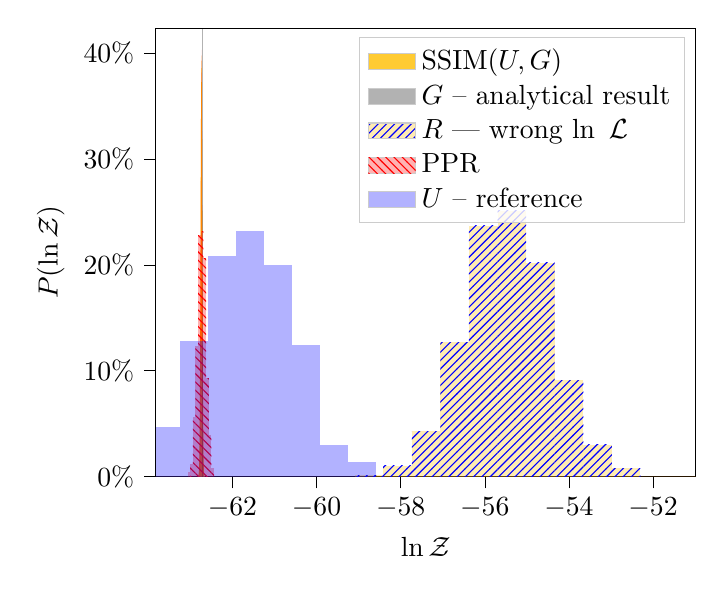
\begin{tikzpicture}

\definecolor{color2}{rgb}{0.0,0.0,1}
\definecolor{color1}{rgb}{1,0.00,0.00}
\definecolor{colorblack}{rgb}{0, 0, 0}
\definecolor{color0}{rgb}{1.0,0.75,0.0}

\begin{axis}[
legend cell align={left},
legend style={fill opacity=0.8, draw opacity=1, text opacity=1, anchor=north east, draw=white!80!black},
tick align=outside,
tick pos=left,
x grid style={white!69.0196078431373!black},
xlabel={\(\ln {\cal Z}\)},
xmin=-63.8198069562379, xmax=-50.9892026507015,
xtick style={color=black},
yticklabel={\pgfmathparse{\tick/10}\pgfmathprintnumber{\pgfmathresult}\%},
y grid style={white!69.0196078431373!black},
ylabel={\(P(\ln {\cal Z})\)},
ymin=0, ymax=423.473092744885,
ytick style={color=black}
]
\path [fill=color0]
(axis cs:-63.8198069562379,0)
--(axis cs:-63.8198069562379,0)
--(axis cs:-63.8069635084846,0)
--(axis cs:-63.7941200607313,0)
--(axis cs:-63.7812766129781,0)
--(axis cs:-63.7684331652248,0)
--(axis cs:-63.7555897174715,0)
--(axis cs:-63.7427462697182,0)
--(axis cs:-63.7299028219649,0)
--(axis cs:-63.7170593742116,0)
--(axis cs:-63.7042159264583,0)
--(axis cs:-63.691372478705,0)
--(axis cs:-63.6785290309517,0)
--(axis cs:-63.6656855831984,0)
--(axis cs:-63.6528421354452,0)
--(axis cs:-63.6399986876919,0)
--(axis cs:-63.6271552399386,0)
--(axis cs:-63.6143117921853,0)
--(axis cs:-63.601468344432,0)
--(axis cs:-63.5886248966787,0)
--(axis cs:-63.5757814489254,0)
--(axis cs:-63.5629380011721,0)
--(axis cs:-63.5500945534188,0)
--(axis cs:-63.5372511056656,0)
--(axis cs:-63.5244076579123,0)
--(axis cs:-63.511564210159,0)
--(axis cs:-63.4987207624057,0)
--(axis cs:-63.4858773146524,0)
--(axis cs:-63.4730338668991,0)
--(axis cs:-63.4601904191458,0)
--(axis cs:-63.4473469713925,0)
--(axis cs:-63.4345035236392,0)
--(axis cs:-63.4216600758859,0)
--(axis cs:-63.4088166281327,0)
--(axis cs:-63.3959731803794,0)
--(axis cs:-63.3831297326261,0)
--(axis cs:-63.3702862848728,0)
--(axis cs:-63.3574428371195,0)
--(axis cs:-63.3445993893662,0)
--(axis cs:-63.3317559416129,0)
--(axis cs:-63.3189124938596,0)
--(axis cs:-63.3060690461063,0)
--(axis cs:-63.293225598353,0)
--(axis cs:-63.2803821505998,0)
--(axis cs:-63.2675387028465,0)
--(axis cs:-63.2546952550932,0)
--(axis cs:-63.2418518073399,0)
--(axis cs:-63.2290083595866,0)
--(axis cs:-63.2161649118333,0)
--(axis cs:-63.20332146408,0)
--(axis cs:-63.1904780163267,0)
--(axis cs:-63.1776345685734,0)
--(axis cs:-63.1647911208201,0)
--(axis cs:-63.1519476730669,0)
--(axis cs:-63.1391042253136,0)
--(axis cs:-63.1262607775603,0)
--(axis cs:-63.113417329807,0)
--(axis cs:-63.1005738820537,0)
--(axis cs:-63.0877304343004,0)
--(axis cs:-63.0748869865471,0)
--(axis cs:-63.0620435387938,0)
--(axis cs:-63.0492000910405,0)
--(axis cs:-63.0363566432872,0)
--(axis cs:-63.023513195534,0)
--(axis cs:-63.0106697477807,0)
--(axis cs:-62.9978263000274,0)
--(axis cs:-62.9849828522741,0)
--(axis cs:-62.9721394045208,0)
--(axis cs:-62.9592959567675,0)
--(axis cs:-62.9464525090142,0)
--(axis cs:-62.9336090612609,0)
--(axis cs:-62.9207656135076,0)
--(axis cs:-62.9079221657544,0)
--(axis cs:-62.8950787180011,0)
--(axis cs:-62.8822352702478,0)
--(axis cs:-62.8693918224945,0)
--(axis cs:-62.8565483747412,0)
--(axis cs:-62.8437049269879,0)
--(axis cs:-62.8308614792346,0)
--(axis cs:-62.8180180314813,0)
--(axis cs:-62.805174583728,0)
--(axis cs:-62.7923311359747,0)
--(axis cs:-62.7794876882215,0)
--(axis cs:-62.7666442404682,0)
--(axis cs:-62.7538007927149,0)
--(axis cs:-62.7409573449616,0)
--(axis cs:-62.7281138972083,0)
--(axis cs:-62.715270449455,0)
--(axis cs:-62.7024270017017,0)
--(axis cs:-62.6895835539484,0)
--(axis cs:-62.6767401061951,0)
--(axis cs:-62.6638966584418,0)
--(axis cs:-62.6510532106886,0)
--(axis cs:-62.6382097629353,0)
--(axis cs:-62.625366315182,0)
--(axis cs:-62.6125228674287,0)
--(axis cs:-62.5996794196754,0)
--(axis cs:-62.5868359719221,0)
--(axis cs:-62.5739925241688,0)
--(axis cs:-62.5611490764155,0)
--(axis cs:-62.5483056286622,0)
--(axis cs:-62.535462180909,0)
--(axis cs:-62.5226187331557,0)
--(axis cs:-62.5097752854024,0)
--(axis cs:-62.4969318376491,0)
--(axis cs:-62.4840883898958,0)
--(axis cs:-62.4712449421425,0)
--(axis cs:-62.4584014943892,0)
--(axis cs:-62.4455580466359,0)
--(axis cs:-62.4327145988826,0)
--(axis cs:-62.4198711511293,0)
--(axis cs:-62.4070277033761,0)
--(axis cs:-62.3941842556228,0)
--(axis cs:-62.3813408078695,0)
--(axis cs:-62.3684973601162,0)
--(axis cs:-62.3556539123629,0)
--(axis cs:-62.3428104646096,0)
--(axis cs:-62.3299670168563,0)
--(axis cs:-62.317123569103,0)
--(axis cs:-62.3042801213497,0)
--(axis cs:-62.2914366735965,0)
--(axis cs:-62.2785932258432,0)
--(axis cs:-62.2657497780899,0)
--(axis cs:-62.2529063303366,0)
--(axis cs:-62.2400628825833,0)
--(axis cs:-62.22721943483,0)
--(axis cs:-62.2143759870767,0)
--(axis cs:-62.2015325393234,0)
--(axis cs:-62.1886890915701,0)
--(axis cs:-62.1758456438168,0)
--(axis cs:-62.1630021960636,0)
--(axis cs:-62.1501587483103,0)
--(axis cs:-62.137315300557,0)
--(axis cs:-62.1244718528037,0)
--(axis cs:-62.1116284050504,0)
--(axis cs:-62.0987849572971,0)
--(axis cs:-62.0859415095438,0)
--(axis cs:-62.0730980617905,0)
--(axis cs:-62.0602546140372,0)
--(axis cs:-62.0474111662839,0)
--(axis cs:-62.0345677185307,0)
--(axis cs:-62.0217242707774,0)
--(axis cs:-62.0088808230241,0)
--(axis cs:-61.9960373752708,0)
--(axis cs:-61.9831939275175,0)
--(axis cs:-61.9703504797642,0)
--(axis cs:-61.9575070320109,0)
--(axis cs:-61.9446635842576,0)
--(axis cs:-61.9318201365043,0)
--(axis cs:-61.918976688751,0)
--(axis cs:-61.9061332409978,0)
--(axis cs:-61.8932897932445,0)
--(axis cs:-61.8804463454912,0)
--(axis cs:-61.8676028977379,0)
--(axis cs:-61.8547594499846,0)
--(axis cs:-61.8419160022313,0)
--(axis cs:-61.829072554478,0)
--(axis cs:-61.8162291067247,0)
--(axis cs:-61.8033856589714,0)
--(axis cs:-61.7905422112181,0)
--(axis cs:-61.7776987634649,0)
--(axis cs:-61.7648553157116,0)
--(axis cs:-61.7520118679583,0)
--(axis cs:-61.739168420205,0)
--(axis cs:-61.7263249724517,0)
--(axis cs:-61.7134815246984,0)
--(axis cs:-61.7006380769451,0)
--(axis cs:-61.6877946291918,0)
--(axis cs:-61.6749511814385,0)
--(axis cs:-61.6621077336853,0)
--(axis cs:-61.649264285932,0)
--(axis cs:-61.6364208381787,0)
--(axis cs:-61.6235773904254,0)
--(axis cs:-61.6107339426721,0)
--(axis cs:-61.5978904949188,0)
--(axis cs:-61.5850470471655,0)
--(axis cs:-61.5722035994122,0)
--(axis cs:-61.5593601516589,0)
--(axis cs:-61.5465167039056,0)
--(axis cs:-61.5336732561524,0)
--(axis cs:-61.5208298083991,0)
--(axis cs:-61.5079863606458,0)
--(axis cs:-61.4951429128925,0)
--(axis cs:-61.4822994651392,0)
--(axis cs:-61.4694560173859,0)
--(axis cs:-61.4566125696326,0)
--(axis cs:-61.4437691218793,0)
--(axis cs:-61.430925674126,0)
--(axis cs:-61.4180822263727,0)
--(axis cs:-61.4052387786195,0)
--(axis cs:-61.3923953308662,0)
--(axis cs:-61.3795518831129,0)
--(axis cs:-61.3667084353596,0)
--(axis cs:-61.3538649876063,0)
--(axis cs:-61.341021539853,0)
--(axis cs:-61.3281780920997,0)
--(axis cs:-61.3153346443464,0)
--(axis cs:-61.3024911965931,0)
--(axis cs:-61.2896477488398,0)
--(axis cs:-61.2768043010866,0)
--(axis cs:-61.2639608533333,0)
--(axis cs:-61.25111740558,0)
--(axis cs:-61.2382739578267,0)
--(axis cs:-61.2254305100734,0)
--(axis cs:-61.2125870623201,0)
--(axis cs:-61.1997436145668,0)
--(axis cs:-61.1869001668135,0)
--(axis cs:-61.1740567190602,0)
--(axis cs:-61.1612132713069,0)
--(axis cs:-61.1483698235537,0)
--(axis cs:-61.1355263758004,0)
--(axis cs:-61.1226829280471,0)
--(axis cs:-61.1098394802938,0)
--(axis cs:-61.0969960325405,0)
--(axis cs:-61.0841525847872,0)
--(axis cs:-61.0713091370339,0)
--(axis cs:-61.0584656892806,0)
--(axis cs:-61.0456222415273,0)
--(axis cs:-61.0327787937741,0)
--(axis cs:-61.0199353460208,0)
--(axis cs:-61.0070918982675,0)
--(axis cs:-60.9942484505142,0)
--(axis cs:-60.9814050027609,0)
--(axis cs:-60.9685615550076,0)
--(axis cs:-60.9557181072543,0)
--(axis cs:-60.942874659501,0)
--(axis cs:-60.9300312117477,0)
--(axis cs:-60.9171877639944,0)
--(axis cs:-60.9043443162412,0)
--(axis cs:-60.8915008684879,0)
--(axis cs:-60.8786574207346,0)
--(axis cs:-60.8658139729813,0)
--(axis cs:-60.852970525228,0)
--(axis cs:-60.8401270774747,0)
--(axis cs:-60.8272836297214,0)
--(axis cs:-60.8144401819681,0)
--(axis cs:-60.8015967342148,0)
--(axis cs:-60.7887532864615,0)
--(axis cs:-60.7759098387083,0)
--(axis cs:-60.763066390955,0)
--(axis cs:-60.7502229432017,0)
--(axis cs:-60.7373794954484,0)
--(axis cs:-60.7245360476951,0)
--(axis cs:-60.7116925999418,0)
--(axis cs:-60.6988491521885,0)
--(axis cs:-60.6860057044352,0)
--(axis cs:-60.6731622566819,0)
--(axis cs:-60.6603188089287,0)
--(axis cs:-60.6474753611754,0)
--(axis cs:-60.6346319134221,0)
--(axis cs:-60.6217884656688,0)
--(axis cs:-60.6089450179155,0)
--(axis cs:-60.5961015701622,0)
--(axis cs:-60.5832581224089,0)
--(axis cs:-60.5704146746556,0)
--(axis cs:-60.5575712269023,0)
--(axis cs:-60.544727779149,0)
--(axis cs:-60.5318843313958,0)
--(axis cs:-60.5190408836425,0)
--(axis cs:-60.5061974358892,0)
--(axis cs:-60.4933539881359,0)
--(axis cs:-60.4805105403826,0)
--(axis cs:-60.4676670926293,0)
--(axis cs:-60.454823644876,0)
--(axis cs:-60.4419801971227,0)
--(axis cs:-60.4291367493694,0)
--(axis cs:-60.4162933016162,0)
--(axis cs:-60.4034498538629,0)
--(axis cs:-60.3906064061096,0)
--(axis cs:-60.3777629583563,0)
--(axis cs:-60.364919510603,0)
--(axis cs:-60.3520760628497,0)
--(axis cs:-60.3392326150964,0)
--(axis cs:-60.3263891673431,0)
--(axis cs:-60.3135457195898,0)
--(axis cs:-60.3007022718365,0)
--(axis cs:-60.2878588240833,0)
--(axis cs:-60.27501537633,0)
--(axis cs:-60.2621719285767,0)
--(axis cs:-60.2493284808234,0)
--(axis cs:-60.2364850330701,0)
--(axis cs:-60.2236415853168,0)
--(axis cs:-60.2107981375635,0)
--(axis cs:-60.1979546898102,0)
--(axis cs:-60.1851112420569,0)
--(axis cs:-60.1722677943036,0)
--(axis cs:-60.1594243465504,0)
--(axis cs:-60.1465808987971,0)
--(axis cs:-60.1337374510438,0)
--(axis cs:-60.1208940032905,0)
--(axis cs:-60.1080505555372,0)
--(axis cs:-60.0952071077839,0)
--(axis cs:-60.0823636600306,0)
--(axis cs:-60.0695202122773,0)
--(axis cs:-60.056676764524,0)
--(axis cs:-60.0438333167707,0)
--(axis cs:-60.0309898690175,0)
--(axis cs:-60.0181464212642,0)
--(axis cs:-60.0053029735109,0)
--(axis cs:-59.9924595257576,0)
--(axis cs:-59.9796160780043,0)
--(axis cs:-59.966772630251,0)
--(axis cs:-59.9539291824977,0)
--(axis cs:-59.9410857347444,0)
--(axis cs:-59.9282422869911,0)
--(axis cs:-59.9153988392378,0)
--(axis cs:-59.9025553914846,0)
--(axis cs:-59.8897119437313,0)
--(axis cs:-59.876868495978,0)
--(axis cs:-59.8640250482247,0)
--(axis cs:-59.8511816004714,0)
--(axis cs:-59.8383381527181,0)
--(axis cs:-59.8254947049648,0)
--(axis cs:-59.8126512572115,0)
--(axis cs:-59.7998078094582,0)
--(axis cs:-59.786964361705,0)
--(axis cs:-59.7741209139517,0)
--(axis cs:-59.7612774661984,0)
--(axis cs:-59.7484340184451,0)
--(axis cs:-59.7355905706918,0)
--(axis cs:-59.7227471229385,0)
--(axis cs:-59.7099036751852,0)
--(axis cs:-59.6970602274319,0)
--(axis cs:-59.6842167796786,0)
--(axis cs:-59.6713733319253,0)
--(axis cs:-59.6585298841721,0)
--(axis cs:-59.6456864364188,0)
--(axis cs:-59.6328429886655,0)
--(axis cs:-59.6199995409122,0)
--(axis cs:-59.6071560931589,0)
--(axis cs:-59.5943126454056,0)
--(axis cs:-59.5814691976523,0)
--(axis cs:-59.568625749899,0)
--(axis cs:-59.5557823021457,0)
--(axis cs:-59.5429388543924,0)
--(axis cs:-59.5300954066392,0)
--(axis cs:-59.5172519588859,0)
--(axis cs:-59.5044085111326,0)
--(axis cs:-59.4915650633793,0)
--(axis cs:-59.478721615626,0)
--(axis cs:-59.4658781678727,0)
--(axis cs:-59.4530347201194,0)
--(axis cs:-59.4401912723661,0)
--(axis cs:-59.4273478246128,0)
--(axis cs:-59.4145043768595,0)
--(axis cs:-59.4016609291063,0)
--(axis cs:-59.388817481353,0)
--(axis cs:-59.3759740335997,0)
--(axis cs:-59.3631305858464,0)
--(axis cs:-59.3502871380931,0)
--(axis cs:-59.3374436903398,0)
--(axis cs:-59.3246002425865,0)
--(axis cs:-59.3117567948332,0)
--(axis cs:-59.2989133470799,0)
--(axis cs:-59.2860698993266,0)
--(axis cs:-59.2732264515734,0)
--(axis cs:-59.2603830038201,0)
--(axis cs:-59.2475395560668,0)
--(axis cs:-59.2346961083135,0)
--(axis cs:-59.2218526605602,0)
--(axis cs:-59.2090092128069,0)
--(axis cs:-59.1961657650536,0)
--(axis cs:-59.1833223173003,0)
--(axis cs:-59.170478869547,0)
--(axis cs:-59.1576354217938,0)
--(axis cs:-59.1447919740405,0)
--(axis cs:-59.1319485262872,0)
--(axis cs:-59.1191050785339,0)
--(axis cs:-59.1062616307806,0)
--(axis cs:-59.0934181830273,0)
--(axis cs:-59.080574735274,0)
--(axis cs:-59.0677312875207,0)
--(axis cs:-59.0548878397674,0)
--(axis cs:-59.0420443920141,0)
--(axis cs:-59.0292009442609,0)
--(axis cs:-59.0163574965076,0)
--(axis cs:-59.0035140487543,0)
--(axis cs:-58.990670601001,0)
--(axis cs:-58.9778271532477,0)
--(axis cs:-58.9649837054944,0)
--(axis cs:-58.9521402577411,0)
--(axis cs:-58.9392968099878,0)
--(axis cs:-58.9264533622345,0)
--(axis cs:-58.9136099144812,0)
--(axis cs:-58.900766466728,0)
--(axis cs:-58.8879230189747,0)
--(axis cs:-58.8750795712214,0)
--(axis cs:-58.8622361234681,0)
--(axis cs:-58.8493926757148,0)
--(axis cs:-58.8365492279615,0)
--(axis cs:-58.8237057802082,0)
--(axis cs:-58.8108623324549,0)
--(axis cs:-58.7980188847016,0)
--(axis cs:-58.7851754369484,0)
--(axis cs:-58.7723319891951,0)
--(axis cs:-58.7594885414418,0)
--(axis cs:-58.7466450936885,0)
--(axis cs:-58.7338016459352,0)
--(axis cs:-58.7209581981819,0)
--(axis cs:-58.7081147504286,0)
--(axis cs:-58.6952713026753,0)
--(axis cs:-58.682427854922,0)
--(axis cs:-58.6695844071687,0)
--(axis cs:-58.6567409594155,0)
--(axis cs:-58.6438975116622,0)
--(axis cs:-58.6310540639089,0)
--(axis cs:-58.6182106161556,0)
--(axis cs:-58.6053671684023,0)
--(axis cs:-58.592523720649,0)
--(axis cs:-58.5796802728957,0)
--(axis cs:-58.5668368251424,0)
--(axis cs:-58.5539933773891,0)
--(axis cs:-58.5411499296358,0)
--(axis cs:-58.5283064818826,0)
--(axis cs:-58.5154630341293,0)
--(axis cs:-58.502619586376,0)
--(axis cs:-58.4897761386227,0)
--(axis cs:-58.4769326908694,0)
--(axis cs:-58.4640892431161,0)
--(axis cs:-58.4512457953628,0)
--(axis cs:-58.4384023476095,0)
--(axis cs:-58.4255588998562,0)
--(axis cs:-58.412715452103,0)
--(axis cs:-58.3998720043497,0)
--(axis cs:-58.3870285565964,0)
--(axis cs:-58.3741851088431,0)
--(axis cs:-58.3613416610898,0)
--(axis cs:-58.3484982133365,0)
--(axis cs:-58.3356547655832,0)
--(axis cs:-58.3228113178299,0)
--(axis cs:-58.3099678700766,0)
--(axis cs:-58.2971244223233,0)
--(axis cs:-58.2842809745701,0)
--(axis cs:-58.2714375268168,0)
--(axis cs:-58.2585940790635,0)
--(axis cs:-58.2457506313102,0)
--(axis cs:-58.2329071835569,0)
--(axis cs:-58.2200637358036,0)
--(axis cs:-58.2072202880503,0)
--(axis cs:-58.194376840297,0)
--(axis cs:-58.1815333925437,0)
--(axis cs:-58.1686899447904,0)
--(axis cs:-58.1558464970372,0)
--(axis cs:-58.1430030492839,0)
--(axis cs:-58.1301596015306,0)
--(axis cs:-58.1173161537773,0)
--(axis cs:-58.104472706024,0)
--(axis cs:-58.0916292582707,0)
--(axis cs:-58.0787858105174,0)
--(axis cs:-58.0659423627641,0)
--(axis cs:-58.0530989150108,0)
--(axis cs:-58.0402554672575,0)
--(axis cs:-58.0274120195043,0)
--(axis cs:-58.014568571751,0)
--(axis cs:-58.0017251239977,0)
--(axis cs:-57.9888816762444,0)
--(axis cs:-57.9760382284911,0)
--(axis cs:-57.9631947807378,0)
--(axis cs:-57.9503513329845,0)
--(axis cs:-57.9375078852312,0)
--(axis cs:-57.9246644374779,0)
--(axis cs:-57.9118209897247,0)
--(axis cs:-57.8989775419714,0)
--(axis cs:-57.8861340942181,0)
--(axis cs:-57.8732906464648,0)
--(axis cs:-57.8604471987115,0)
--(axis cs:-57.8476037509582,0)
--(axis cs:-57.8347603032049,0)
--(axis cs:-57.8219168554516,0)
--(axis cs:-57.8090734076983,0)
--(axis cs:-57.796229959945,0)
--(axis cs:-57.7833865121918,0)
--(axis cs:-57.7705430644385,0)
--(axis cs:-57.7576996166852,0)
--(axis cs:-57.7448561689319,0)
--(axis cs:-57.7320127211786,0)
--(axis cs:-57.7191692734253,0)
--(axis cs:-57.706325825672,0)
--(axis cs:-57.6934823779187,0)
--(axis cs:-57.6806389301654,0)
--(axis cs:-57.6677954824121,0)
--(axis cs:-57.6549520346589,0)
--(axis cs:-57.6421085869056,0)
--(axis cs:-57.6292651391523,0)
--(axis cs:-57.616421691399,0)
--(axis cs:-57.6035782436457,0)
--(axis cs:-57.5907347958924,0)
--(axis cs:-57.5778913481391,0)
--(axis cs:-57.5650479003858,0)
--(axis cs:-57.5522044526325,0)
--(axis cs:-57.5393610048792,0)
--(axis cs:-57.526517557126,0)
--(axis cs:-57.5136741093727,0)
--(axis cs:-57.5008306616194,0)
--(axis cs:-57.4879872138661,0)
--(axis cs:-57.4751437661128,0)
--(axis cs:-57.4623003183595,0)
--(axis cs:-57.4494568706062,0)
--(axis cs:-57.4366134228529,0)
--(axis cs:-57.4237699750996,0)
--(axis cs:-57.4109265273463,0)
--(axis cs:-57.3980830795931,0)
--(axis cs:-57.3852396318398,0)
--(axis cs:-57.3723961840865,0)
--(axis cs:-57.3595527363332,0)
--(axis cs:-57.3467092885799,0)
--(axis cs:-57.3338658408266,0)
--(axis cs:-57.3210223930733,0)
--(axis cs:-57.30817894532,0)
--(axis cs:-57.2953354975667,0)
--(axis cs:-57.2824920498135,0)
--(axis cs:-57.2696486020602,0)
--(axis cs:-57.2568051543069,0)
--(axis cs:-57.2439617065536,0)
--(axis cs:-57.2311182588003,0)
--(axis cs:-57.218274811047,0)
--(axis cs:-57.2054313632937,0)
--(axis cs:-57.1925879155404,0)
--(axis cs:-57.1797444677871,0)
--(axis cs:-57.1669010200338,0)
--(axis cs:-57.1540575722806,0)
--(axis cs:-57.1412141245273,0)
--(axis cs:-57.128370676774,0)
--(axis cs:-57.1155272290207,0)
--(axis cs:-57.1026837812674,0)
--(axis cs:-57.0898403335141,0)
--(axis cs:-57.0769968857608,0)
--(axis cs:-57.0641534380075,0)
--(axis cs:-57.0513099902542,0)
--(axis cs:-57.0384665425009,0)
--(axis cs:-57.0256230947477,0)
--(axis cs:-57.0127796469944,0)
--(axis cs:-56.9999361992411,0)
--(axis cs:-56.9870927514878,0)
--(axis cs:-56.9742493037345,0)
--(axis cs:-56.9614058559812,0)
--(axis cs:-56.9485624082279,0)
--(axis cs:-56.9357189604746,0)
--(axis cs:-56.9228755127213,0)
--(axis cs:-56.910032064968,0)
--(axis cs:-56.8971886172148,0)
--(axis cs:-56.8843451694615,0)
--(axis cs:-56.8715017217082,0)
--(axis cs:-56.8586582739549,0)
--(axis cs:-56.8458148262016,0)
--(axis cs:-56.8329713784483,0)
--(axis cs:-56.820127930695,0)
--(axis cs:-56.8072844829417,0)
--(axis cs:-56.7944410351884,0)
--(axis cs:-56.7815975874352,0)
--(axis cs:-56.7687541396819,0)
--(axis cs:-56.7559106919286,0)
--(axis cs:-56.7430672441753,0)
--(axis cs:-56.730223796422,0)
--(axis cs:-56.7173803486687,0)
--(axis cs:-56.7045369009154,0)
--(axis cs:-56.6916934531621,0)
--(axis cs:-56.6788500054088,0)
--(axis cs:-56.6660065576555,0)
--(axis cs:-56.6531631099023,0)
--(axis cs:-56.640319662149,0)
--(axis cs:-56.6274762143957,0)
--(axis cs:-56.6146327666424,0)
--(axis cs:-56.6017893188891,0)
--(axis cs:-56.5889458711358,0)
--(axis cs:-56.5761024233825,0)
--(axis cs:-56.5632589756292,0)
--(axis cs:-56.5504155278759,0)
--(axis cs:-56.5375720801227,0)
--(axis cs:-56.5247286323694,0)
--(axis cs:-56.5118851846161,0)
--(axis cs:-56.4990417368628,0)
--(axis cs:-56.4861982891095,0)
--(axis cs:-56.4733548413562,0)
--(axis cs:-56.4605113936029,0)
--(axis cs:-56.4476679458496,0)
--(axis cs:-56.4348244980963,0)
--(axis cs:-56.421981050343,0)
--(axis cs:-56.4091376025898,0)
--(axis cs:-56.3962941548365,0)
--(axis cs:-56.3834507070832,0)
--(axis cs:-56.3706072593299,0)
--(axis cs:-56.3577638115766,0)
--(axis cs:-56.3449203638233,0)
--(axis cs:-56.33207691607,0)
--(axis cs:-56.3192334683167,0)
--(axis cs:-56.3063900205634,0)
--(axis cs:-56.2935465728101,0)
--(axis cs:-56.2807031250569,0)
--(axis cs:-56.2678596773036,0)
--(axis cs:-56.2550162295503,0)
--(axis cs:-56.242172781797,0)
--(axis cs:-56.2293293340437,0)
--(axis cs:-56.2164858862904,0)
--(axis cs:-56.2036424385371,0)
--(axis cs:-56.1907989907838,0)
--(axis cs:-56.1779555430305,0)
--(axis cs:-56.1651120952772,0)
--(axis cs:-56.152268647524,0)
--(axis cs:-56.1394251997707,0)
--(axis cs:-56.1265817520174,0)
--(axis cs:-56.1137383042641,0)
--(axis cs:-56.1008948565108,0)
--(axis cs:-56.0880514087575,0)
--(axis cs:-56.0752079610042,0)
--(axis cs:-56.0623645132509,0)
--(axis cs:-56.0495210654976,0)
--(axis cs:-56.0366776177444,0)
--(axis cs:-56.0238341699911,0)
--(axis cs:-56.0109907222378,0)
--(axis cs:-55.9981472744845,0)
--(axis cs:-55.9853038267312,0)
--(axis cs:-55.9724603789779,0)
--(axis cs:-55.9596169312246,0)
--(axis cs:-55.9467734834713,0)
--(axis cs:-55.933930035718,0)
--(axis cs:-55.9210865879647,0)
--(axis cs:-55.9082431402115,0)
--(axis cs:-55.8953996924582,0)
--(axis cs:-55.8825562447049,0)
--(axis cs:-55.8697127969516,0)
--(axis cs:-55.8568693491983,0)
--(axis cs:-55.844025901445,0)
--(axis cs:-55.8311824536917,0)
--(axis cs:-55.8183390059384,0)
--(axis cs:-55.8054955581851,0)
--(axis cs:-55.7926521104318,0)
--(axis cs:-55.7798086626786,0)
--(axis cs:-55.7669652149253,0)
--(axis cs:-55.754121767172,0)
--(axis cs:-55.7412783194187,0)
--(axis cs:-55.7284348716654,0)
--(axis cs:-55.7155914239121,0)
--(axis cs:-55.7027479761588,0)
--(axis cs:-55.6899045284055,0)
--(axis cs:-55.6770610806522,0)
--(axis cs:-55.6642176328989,0)
--(axis cs:-55.6513741851457,0)
--(axis cs:-55.6385307373924,0)
--(axis cs:-55.6256872896391,0)
--(axis cs:-55.6128438418858,0)
--(axis cs:-55.6000003941325,0)
--(axis cs:-55.5871569463792,0)
--(axis cs:-55.5743134986259,0)
--(axis cs:-55.5614700508726,0)
--(axis cs:-55.5486266031193,0)
--(axis cs:-55.535783155366,0)
--(axis cs:-55.5229397076128,0)
--(axis cs:-55.5100962598595,0)
--(axis cs:-55.4972528121062,0)
--(axis cs:-55.4844093643529,0)
--(axis cs:-55.4715659165996,0)
--(axis cs:-55.4587224688463,0)
--(axis cs:-55.445879021093,0)
--(axis cs:-55.4330355733397,0)
--(axis cs:-55.4201921255864,0)
--(axis cs:-55.4073486778332,0)
--(axis cs:-55.3945052300799,0)
--(axis cs:-55.3816617823266,0)
--(axis cs:-55.3688183345733,0)
--(axis cs:-55.35597488682,0)
--(axis cs:-55.3431314390667,0)
--(axis cs:-55.3302879913134,0)
--(axis cs:-55.3174445435601,0)
--(axis cs:-55.3046010958068,0)
--(axis cs:-55.2917576480535,0)
--(axis cs:-55.2789142003003,0)
--(axis cs:-55.266070752547,0)
--(axis cs:-55.2532273047937,0)
--(axis cs:-55.2403838570404,0)
--(axis cs:-55.2275404092871,0)
--(axis cs:-55.2146969615338,0)
--(axis cs:-55.2018535137805,0)
--(axis cs:-55.1890100660272,0)
--(axis cs:-55.1761666182739,0)
--(axis cs:-55.1633231705206,0)
--(axis cs:-55.1504797227674,0)
--(axis cs:-55.1376362750141,0)
--(axis cs:-55.1247928272608,0)
--(axis cs:-55.1119493795075,0)
--(axis cs:-55.0991059317542,0)
--(axis cs:-55.0862624840009,0)
--(axis cs:-55.0734190362476,0)
--(axis cs:-55.0605755884943,0)
--(axis cs:-55.047732140741,0)
--(axis cs:-55.0348886929877,0)
--(axis cs:-55.0220452452345,0)
--(axis cs:-55.0092017974812,0)
--(axis cs:-54.9963583497279,0)
--(axis cs:-54.9835149019746,0)
--(axis cs:-54.9706714542213,0)
--(axis cs:-54.957828006468,0)
--(axis cs:-54.9449845587147,0)
--(axis cs:-54.9321411109614,0)
--(axis cs:-54.9192976632081,0)
--(axis cs:-54.9064542154549,0)
--(axis cs:-54.8936107677016,0)
--(axis cs:-54.8807673199483,0)
--(axis cs:-54.867923872195,0)
--(axis cs:-54.8550804244417,0)
--(axis cs:-54.8422369766884,0)
--(axis cs:-54.8293935289351,0)
--(axis cs:-54.8165500811818,0)
--(axis cs:-54.8037066334285,0)
--(axis cs:-54.7908631856752,0)
--(axis cs:-54.778019737922,0)
--(axis cs:-54.7651762901687,0)
--(axis cs:-54.7523328424154,0)
--(axis cs:-54.7394893946621,0)
--(axis cs:-54.7266459469088,0)
--(axis cs:-54.7138024991555,0)
--(axis cs:-54.7009590514022,0)
--(axis cs:-54.6881156036489,0)
--(axis cs:-54.6752721558956,0)
--(axis cs:-54.6624287081424,0)
--(axis cs:-54.6495852603891,0)
--(axis cs:-54.6367418126358,0)
--(axis cs:-54.6238983648825,0)
--(axis cs:-54.6110549171292,0)
--(axis cs:-54.5982114693759,0)
--(axis cs:-54.5853680216226,0)
--(axis cs:-54.5725245738693,0)
--(axis cs:-54.559681126116,0)
--(axis cs:-54.5468376783627,0)
--(axis cs:-54.5339942306095,0)
--(axis cs:-54.5211507828562,0)
--(axis cs:-54.5083073351029,0)
--(axis cs:-54.4954638873496,0)
--(axis cs:-54.4826204395963,0)
--(axis cs:-54.469776991843,0)
--(axis cs:-54.4569335440897,0)
--(axis cs:-54.4440900963364,0)
--(axis cs:-54.4312466485831,0)
--(axis cs:-54.4184032008298,0)
--(axis cs:-54.4055597530766,0)
--(axis cs:-54.3927163053233,0)
--(axis cs:-54.37987285757,0)
--(axis cs:-54.3670294098167,0)
--(axis cs:-54.3541859620634,0)
--(axis cs:-54.3413425143101,0)
--(axis cs:-54.3284990665568,0)
--(axis cs:-54.3156556188035,0)
--(axis cs:-54.3028121710502,0)
--(axis cs:-54.2899687232969,0)
--(axis cs:-54.2771252755437,0)
--(axis cs:-54.2642818277904,0)
--(axis cs:-54.2514383800371,0)
--(axis cs:-54.2385949322838,0)
--(axis cs:-54.2257514845305,0)
--(axis cs:-54.2129080367772,0)
--(axis cs:-54.2000645890239,0)
--(axis cs:-54.1872211412706,0)
--(axis cs:-54.1743776935173,0)
--(axis cs:-54.161534245764,0)
--(axis cs:-54.1486907980108,0)
--(axis cs:-54.1358473502575,0)
--(axis cs:-54.1230039025042,0)
--(axis cs:-54.1101604547509,0)
--(axis cs:-54.0973170069976,0)
--(axis cs:-54.0844735592443,0)
--(axis cs:-54.071630111491,0)
--(axis cs:-54.0587866637377,0)
--(axis cs:-54.0459432159844,0)
--(axis cs:-54.0330997682312,0)
--(axis cs:-54.0202563204779,0)
--(axis cs:-54.0074128727246,0)
--(axis cs:-53.9945694249713,0)
--(axis cs:-53.981725977218,0)
--(axis cs:-53.9688825294647,0)
--(axis cs:-53.9560390817114,0)
--(axis cs:-53.9431956339581,0)
--(axis cs:-53.9303521862048,0)
--(axis cs:-53.9175087384515,0)
--(axis cs:-53.9046652906983,0)
--(axis cs:-53.891821842945,0)
--(axis cs:-53.8789783951917,0)
--(axis cs:-53.8661349474384,0)
--(axis cs:-53.8532914996851,0)
--(axis cs:-53.8404480519318,0)
--(axis cs:-53.8276046041785,0)
--(axis cs:-53.8147611564252,0)
--(axis cs:-53.8019177086719,0)
--(axis cs:-53.7890742609186,0)
--(axis cs:-53.7762308131654,0)
--(axis cs:-53.7633873654121,0)
--(axis cs:-53.7505439176588,0)
--(axis cs:-53.7377004699055,0)
--(axis cs:-53.7248570221522,0)
--(axis cs:-53.7120135743989,0)
--(axis cs:-53.6991701266456,0)
--(axis cs:-53.6863266788923,0)
--(axis cs:-53.673483231139,0)
--(axis cs:-53.6606397833857,0)
--(axis cs:-53.6477963356325,0)
--(axis cs:-53.6349528878792,0)
--(axis cs:-53.6221094401259,0)
--(axis cs:-53.6092659923726,0)
--(axis cs:-53.5964225446193,0)
--(axis cs:-53.583579096866,0)
--(axis cs:-53.5707356491127,0)
--(axis cs:-53.5578922013594,0)
--(axis cs:-53.5450487536061,0)
--(axis cs:-53.5322053058529,0)
--(axis cs:-53.5193618580996,0)
--(axis cs:-53.5065184103463,0)
--(axis cs:-53.493674962593,0)
--(axis cs:-53.4808315148397,0)
--(axis cs:-53.4679880670864,0)
--(axis cs:-53.4551446193331,0)
--(axis cs:-53.4423011715798,0)
--(axis cs:-53.4294577238265,0)
--(axis cs:-53.4166142760732,0)
--(axis cs:-53.40377082832,0)
--(axis cs:-53.3909273805667,0)
--(axis cs:-53.3780839328134,0)
--(axis cs:-53.3652404850601,0)
--(axis cs:-53.3523970373068,0)
--(axis cs:-53.3395535895535,0)
--(axis cs:-53.3267101418002,0)
--(axis cs:-53.3138666940469,0)
--(axis cs:-53.3010232462936,0)
--(axis cs:-53.2881797985403,0)
--(axis cs:-53.2753363507871,0)
--(axis cs:-53.2624929030338,0)
--(axis cs:-53.2496494552805,0)
--(axis cs:-53.2368060075272,0)
--(axis cs:-53.2239625597739,0)
--(axis cs:-53.2111191120206,0)
--(axis cs:-53.1982756642673,0)
--(axis cs:-53.185432216514,0)
--(axis cs:-53.1725887687607,0)
--(axis cs:-53.1597453210074,0)
--(axis cs:-53.1469018732542,0)
--(axis cs:-53.1340584255009,0)
--(axis cs:-53.1212149777476,0)
--(axis cs:-53.1083715299943,0)
--(axis cs:-53.095528082241,0)
--(axis cs:-53.0826846344877,0)
--(axis cs:-53.0698411867344,0)
--(axis cs:-53.0569977389811,0)
--(axis cs:-53.0441542912278,0)
--(axis cs:-53.0313108434746,0)
--(axis cs:-53.0184673957213,0)
--(axis cs:-53.005623947968,0)
--(axis cs:-52.9927805002147,0)
--(axis cs:-52.9799370524614,0)
--(axis cs:-52.9670936047081,0)
--(axis cs:-52.9542501569548,0)
--(axis cs:-52.9414067092015,0)
--(axis cs:-52.9285632614482,0)
--(axis cs:-52.9157198136949,0)
--(axis cs:-52.9028763659417,0)
--(axis cs:-52.8900329181884,0)
--(axis cs:-52.8771894704351,0)
--(axis cs:-52.8643460226818,0)
--(axis cs:-52.8515025749285,0)
--(axis cs:-52.8386591271752,0)
--(axis cs:-52.8258156794219,0)
--(axis cs:-52.8129722316686,0)
--(axis cs:-52.8001287839153,0)
--(axis cs:-52.787285336162,0)
--(axis cs:-52.7744418884088,0)
--(axis cs:-52.7615984406555,0)
--(axis cs:-52.7487549929022,0)
--(axis cs:-52.7359115451489,0)
--(axis cs:-52.7230680973956,0)
--(axis cs:-52.7102246496423,0)
--(axis cs:-52.697381201889,0)
--(axis cs:-52.6845377541357,0)
--(axis cs:-52.6716943063824,0)
--(axis cs:-52.6588508586292,0)
--(axis cs:-52.6460074108759,0)
--(axis cs:-52.6331639631226,0)
--(axis cs:-52.6203205153693,0)
--(axis cs:-52.607477067616,0)
--(axis cs:-52.5946336198627,0)
--(axis cs:-52.5817901721094,0)
--(axis cs:-52.5689467243561,0)
--(axis cs:-52.5561032766028,0)
--(axis cs:-52.5432598288495,0)
--(axis cs:-52.5304163810963,0)
--(axis cs:-52.517572933343,0)
--(axis cs:-52.5047294855897,0)
--(axis cs:-52.4918860378364,0)
--(axis cs:-52.4790425900831,0)
--(axis cs:-52.4661991423298,0)
--(axis cs:-52.4533556945765,0)
--(axis cs:-52.4405122468232,0)
--(axis cs:-52.4276687990699,0)
--(axis cs:-52.4148253513166,0)
--(axis cs:-52.4019819035634,0)
--(axis cs:-52.3891384558101,0)
--(axis cs:-52.3762950080568,0)
--(axis cs:-52.3634515603035,0)
--(axis cs:-52.3506081125502,0)
--(axis cs:-52.3377646647969,0)
--(axis cs:-52.3249212170436,0)
--(axis cs:-52.3120777692903,0)
--(axis cs:-52.299234321537,0)
--(axis cs:-52.2863908737837,0)
--(axis cs:-52.2735474260305,0)
--(axis cs:-52.2607039782772,0)
--(axis cs:-52.2478605305239,0)
--(axis cs:-52.2350170827706,0)
--(axis cs:-52.2221736350173,0)
--(axis cs:-52.209330187264,0)
--(axis cs:-52.1964867395107,0)
--(axis cs:-52.1836432917574,0)
--(axis cs:-52.1707998440041,0)
--(axis cs:-52.1579563962509,0)
--(axis cs:-52.1451129484976,0)
--(axis cs:-52.1322695007443,0)
--(axis cs:-52.119426052991,0)
--(axis cs:-52.1065826052377,0)
--(axis cs:-52.0937391574844,0)
--(axis cs:-52.0808957097311,0)
--(axis cs:-52.0680522619778,0)
--(axis cs:-52.0552088142245,0)
--(axis cs:-52.0423653664712,0)
--(axis cs:-52.029521918718,0)
--(axis cs:-52.0166784709647,0)
--(axis cs:-52.0038350232114,0)
--(axis cs:-51.9909915754581,0)
--(axis cs:-51.9781481277048,0)
--(axis cs:-51.9653046799515,0)
--(axis cs:-51.9524612321982,0)
--(axis cs:-51.9396177844449,0)
--(axis cs:-51.9267743366916,0)
--(axis cs:-51.9139308889383,0)
--(axis cs:-51.9010874411851,0)
--(axis cs:-51.8882439934318,0)
--(axis cs:-51.8754005456785,0)
--(axis cs:-51.8625570979252,0)
--(axis cs:-51.8497136501719,0)
--(axis cs:-51.8368702024186,0)
--(axis cs:-51.8240267546653,0)
--(axis cs:-51.811183306912,0)
--(axis cs:-51.7983398591587,0)
--(axis cs:-51.7854964114054,0)
--(axis cs:-51.7726529636522,0)
--(axis cs:-51.7598095158989,0)
--(axis cs:-51.7469660681456,0)
--(axis cs:-51.7341226203923,0)
--(axis cs:-51.721279172639,0)
--(axis cs:-51.7084357248857,0)
--(axis cs:-51.6955922771324,0)
--(axis cs:-51.6827488293791,0)
--(axis cs:-51.6699053816258,0)
--(axis cs:-51.6570619338726,0)
--(axis cs:-51.6442184861193,0)
--(axis cs:-51.631375038366,0)
--(axis cs:-51.6185315906127,0)
--(axis cs:-51.6056881428594,0)
--(axis cs:-51.5928446951061,0)
--(axis cs:-51.5800012473528,0)
--(axis cs:-51.5671577995995,0)
--(axis cs:-51.5543143518462,0)
--(axis cs:-51.5414709040929,0)
--(axis cs:-51.5286274563397,0)
--(axis cs:-51.5157840085864,0)
--(axis cs:-51.5029405608331,0)
--(axis cs:-51.4900971130798,0)
--(axis cs:-51.4772536653265,0)
--(axis cs:-51.4644102175732,0)
--(axis cs:-51.4515667698199,0)
--(axis cs:-51.4387233220666,0)
--(axis cs:-51.4258798743133,0)
--(axis cs:-51.41303642656,0)
--(axis cs:-51.4001929788068,0)
--(axis cs:-51.3873495310535,0)
--(axis cs:-51.3745060833002,0)
--(axis cs:-51.3616626355469,0)
--(axis cs:-51.3488191877936,0)
--(axis cs:-51.3359757400403,0)
--(axis cs:-51.323132292287,0)
--(axis cs:-51.3102888445337,0)
--(axis cs:-51.2974453967804,0)
--(axis cs:-51.2846019490271,0)
--(axis cs:-51.2717585012739,0)
--(axis cs:-51.2589150535206,0)
--(axis cs:-51.2460716057673,0)
--(axis cs:-51.233228158014,0)
--(axis cs:-51.2203847102607,0)
--(axis cs:-51.2075412625074,0)
--(axis cs:-51.1946978147541,0)
--(axis cs:-51.1818543670008,0)
--(axis cs:-51.1690109192475,0)
--(axis cs:-51.1561674714942,0)
--(axis cs:-51.143324023741,0)
--(axis cs:-51.1304805759877,0)
--(axis cs:-51.1176371282344,0)
--(axis cs:-51.1047936804811,0)
--(axis cs:-51.0919502327278,0)
--(axis cs:-51.0791067849745,0)
--(axis cs:-51.0662633372212,0)
--(axis cs:-51.0534198894679,0)
--(axis cs:-51.0405764417146,0)
--(axis cs:-51.0277329939614,0)
--(axis cs:-51.0148895462081,0)
--(axis cs:-51.0020460984548,0)
--(axis cs:-50.9892026507015,0)
--(axis cs:-50.9892026507015,0)
--(axis cs:-50.9892026507015,0)
--(axis cs:-51.0020460984548,0)
--(axis cs:-51.0148895462081,0)
--(axis cs:-51.0277329939614,0)
--(axis cs:-51.0405764417146,0)
--(axis cs:-51.0534198894679,0)
--(axis cs:-51.0662633372212,0)
--(axis cs:-51.0791067849745,0)
--(axis cs:-51.0919502327278,0)
--(axis cs:-51.1047936804811,0)
--(axis cs:-51.1176371282344,0)
--(axis cs:-51.1304805759877,0)
--(axis cs:-51.143324023741,0)
--(axis cs:-51.1561674714942,0)
--(axis cs:-51.1690109192475,0)
--(axis cs:-51.1818543670008,0)
--(axis cs:-51.1946978147541,0)
--(axis cs:-51.2075412625074,0)
--(axis cs:-51.2203847102607,0)
--(axis cs:-51.233228158014,0)
--(axis cs:-51.2460716057673,0)
--(axis cs:-51.2589150535206,0)
--(axis cs:-51.2717585012739,0)
--(axis cs:-51.2846019490271,0)
--(axis cs:-51.2974453967804,0)
--(axis cs:-51.3102888445337,0)
--(axis cs:-51.323132292287,0)
--(axis cs:-51.3359757400403,0)
--(axis cs:-51.3488191877936,0)
--(axis cs:-51.3616626355469,0)
--(axis cs:-51.3745060833002,0)
--(axis cs:-51.3873495310535,0)
--(axis cs:-51.4001929788068,0)
--(axis cs:-51.41303642656,0)
--(axis cs:-51.4258798743133,0)
--(axis cs:-51.4387233220666,0)
--(axis cs:-51.4515667698199,0)
--(axis cs:-51.4644102175732,0)
--(axis cs:-51.4772536653265,0)
--(axis cs:-51.4900971130798,0)
--(axis cs:-51.5029405608331,0)
--(axis cs:-51.5157840085864,0)
--(axis cs:-51.5286274563397,0)
--(axis cs:-51.5414709040929,0)
--(axis cs:-51.5543143518462,0)
--(axis cs:-51.5671577995995,0)
--(axis cs:-51.5800012473528,0)
--(axis cs:-51.5928446951061,0)
--(axis cs:-51.6056881428594,0)
--(axis cs:-51.6185315906127,0)
--(axis cs:-51.631375038366,0)
--(axis cs:-51.6442184861193,0)
--(axis cs:-51.6570619338726,0)
--(axis cs:-51.6699053816258,0)
--(axis cs:-51.6827488293791,0)
--(axis cs:-51.6955922771324,0)
--(axis cs:-51.7084357248857,0)
--(axis cs:-51.721279172639,0)
--(axis cs:-51.7341226203923,0)
--(axis cs:-51.7469660681456,0)
--(axis cs:-51.7598095158989,0)
--(axis cs:-51.7726529636522,0)
--(axis cs:-51.7854964114054,0)
--(axis cs:-51.7983398591587,0)
--(axis cs:-51.811183306912,0)
--(axis cs:-51.8240267546653,0)
--(axis cs:-51.8368702024186,0)
--(axis cs:-51.8497136501719,0)
--(axis cs:-51.8625570979252,0)
--(axis cs:-51.8754005456785,0)
--(axis cs:-51.8882439934318,0)
--(axis cs:-51.9010874411851,0)
--(axis cs:-51.9139308889383,0)
--(axis cs:-51.9267743366916,0)
--(axis cs:-51.9396177844449,0)
--(axis cs:-51.9524612321982,0)
--(axis cs:-51.9653046799515,0)
--(axis cs:-51.9781481277048,0)
--(axis cs:-51.9909915754581,0)
--(axis cs:-52.0038350232114,0)
--(axis cs:-52.0166784709647,0)
--(axis cs:-52.029521918718,0)
--(axis cs:-52.0423653664712,0)
--(axis cs:-52.0552088142245,0)
--(axis cs:-52.0680522619778,0)
--(axis cs:-52.0808957097311,0)
--(axis cs:-52.0937391574844,0)
--(axis cs:-52.1065826052377,0)
--(axis cs:-52.119426052991,0)
--(axis cs:-52.1322695007443,0)
--(axis cs:-52.1451129484976,0)
--(axis cs:-52.1579563962509,0)
--(axis cs:-52.1707998440041,0)
--(axis cs:-52.1836432917574,0)
--(axis cs:-52.1964867395107,0)
--(axis cs:-52.209330187264,0)
--(axis cs:-52.2221736350173,0)
--(axis cs:-52.2350170827706,0)
--(axis cs:-52.2478605305239,0)
--(axis cs:-52.2607039782772,0)
--(axis cs:-52.2735474260305,0)
--(axis cs:-52.2863908737837,0)
--(axis cs:-52.299234321537,0)
--(axis cs:-52.3120777692903,0)
--(axis cs:-52.3249212170436,0)
--(axis cs:-52.3377646647969,0)
--(axis cs:-52.3506081125502,0)
--(axis cs:-52.3634515603035,0)
--(axis cs:-52.3762950080568,0)
--(axis cs:-52.3891384558101,0)
--(axis cs:-52.4019819035634,0)
--(axis cs:-52.4148253513166,0)
--(axis cs:-52.4276687990699,0)
--(axis cs:-52.4405122468232,0)
--(axis cs:-52.4533556945765,0)
--(axis cs:-52.4661991423298,0)
--(axis cs:-52.4790425900831,0)
--(axis cs:-52.4918860378364,0)
--(axis cs:-52.5047294855897,0)
--(axis cs:-52.517572933343,0)
--(axis cs:-52.5304163810963,0)
--(axis cs:-52.5432598288495,0)
--(axis cs:-52.5561032766028,0)
--(axis cs:-52.5689467243561,0)
--(axis cs:-52.5817901721094,0)
--(axis cs:-52.5946336198627,0)
--(axis cs:-52.607477067616,0)
--(axis cs:-52.6203205153693,0)
--(axis cs:-52.6331639631226,0)
--(axis cs:-52.6460074108759,0)
--(axis cs:-52.6588508586292,0)
--(axis cs:-52.6716943063824,0)
--(axis cs:-52.6845377541357,0)
--(axis cs:-52.697381201889,0)
--(axis cs:-52.7102246496423,0)
--(axis cs:-52.7230680973956,0)
--(axis cs:-52.7359115451489,0)
--(axis cs:-52.7487549929022,0)
--(axis cs:-52.7615984406555,0)
--(axis cs:-52.7744418884088,0)
--(axis cs:-52.787285336162,0)
--(axis cs:-52.8001287839153,0)
--(axis cs:-52.8129722316686,0)
--(axis cs:-52.8258156794219,0)
--(axis cs:-52.8386591271752,0)
--(axis cs:-52.8515025749285,0)
--(axis cs:-52.8643460226818,0)
--(axis cs:-52.8771894704351,0)
--(axis cs:-52.8900329181884,0)
--(axis cs:-52.9028763659417,0)
--(axis cs:-52.9157198136949,0)
--(axis cs:-52.9285632614482,0)
--(axis cs:-52.9414067092015,0)
--(axis cs:-52.9542501569548,0)
--(axis cs:-52.9670936047081,0)
--(axis cs:-52.9799370524614,0)
--(axis cs:-52.9927805002147,0)
--(axis cs:-53.005623947968,0)
--(axis cs:-53.0184673957213,0)
--(axis cs:-53.0313108434746,0)
--(axis cs:-53.0441542912278,0)
--(axis cs:-53.0569977389811,0)
--(axis cs:-53.0698411867344,0)
--(axis cs:-53.0826846344877,0)
--(axis cs:-53.095528082241,0)
--(axis cs:-53.1083715299943,0)
--(axis cs:-53.1212149777476,0)
--(axis cs:-53.1340584255009,0)
--(axis cs:-53.1469018732542,0)
--(axis cs:-53.1597453210074,0)
--(axis cs:-53.1725887687607,0)
--(axis cs:-53.185432216514,0)
--(axis cs:-53.1982756642673,0)
--(axis cs:-53.2111191120206,0)
--(axis cs:-53.2239625597739,0)
--(axis cs:-53.2368060075272,0)
--(axis cs:-53.2496494552805,0)
--(axis cs:-53.2624929030338,0)
--(axis cs:-53.2753363507871,0)
--(axis cs:-53.2881797985403,0)
--(axis cs:-53.3010232462936,0)
--(axis cs:-53.3138666940469,0)
--(axis cs:-53.3267101418002,0)
--(axis cs:-53.3395535895535,0)
--(axis cs:-53.3523970373068,0)
--(axis cs:-53.3652404850601,0)
--(axis cs:-53.3780839328134,0)
--(axis cs:-53.3909273805667,0)
--(axis cs:-53.40377082832,0)
--(axis cs:-53.4166142760732,0)
--(axis cs:-53.4294577238265,0)
--(axis cs:-53.4423011715798,0)
--(axis cs:-53.4551446193331,0)
--(axis cs:-53.4679880670864,0)
--(axis cs:-53.4808315148397,0)
--(axis cs:-53.493674962593,0)
--(axis cs:-53.5065184103463,0)
--(axis cs:-53.5193618580996,0)
--(axis cs:-53.5322053058529,0)
--(axis cs:-53.5450487536061,0)
--(axis cs:-53.5578922013594,0)
--(axis cs:-53.5707356491127,0)
--(axis cs:-53.583579096866,0)
--(axis cs:-53.5964225446193,0)
--(axis cs:-53.6092659923726,0)
--(axis cs:-53.6221094401259,0)
--(axis cs:-53.6349528878792,0)
--(axis cs:-53.6477963356325,0)
--(axis cs:-53.6606397833857,0)
--(axis cs:-53.673483231139,0)
--(axis cs:-53.6863266788923,0)
--(axis cs:-53.6991701266456,0)
--(axis cs:-53.7120135743989,0)
--(axis cs:-53.7248570221522,0)
--(axis cs:-53.7377004699055,0)
--(axis cs:-53.7505439176588,0)
--(axis cs:-53.7633873654121,0)
--(axis cs:-53.7762308131654,0)
--(axis cs:-53.7890742609186,0)
--(axis cs:-53.8019177086719,0)
--(axis cs:-53.8147611564252,0)
--(axis cs:-53.8276046041785,0)
--(axis cs:-53.8404480519318,0)
--(axis cs:-53.8532914996851,0)
--(axis cs:-53.8661349474384,0)
--(axis cs:-53.8789783951917,0)
--(axis cs:-53.891821842945,0)
--(axis cs:-53.9046652906983,0)
--(axis cs:-53.9175087384515,0)
--(axis cs:-53.9303521862048,0)
--(axis cs:-53.9431956339581,0)
--(axis cs:-53.9560390817114,0)
--(axis cs:-53.9688825294647,0)
--(axis cs:-53.981725977218,0)
--(axis cs:-53.9945694249713,0)
--(axis cs:-54.0074128727246,0)
--(axis cs:-54.0202563204779,0)
--(axis cs:-54.0330997682312,0)
--(axis cs:-54.0459432159844,0)
--(axis cs:-54.0587866637377,0)
--(axis cs:-54.071630111491,0)
--(axis cs:-54.0844735592443,0)
--(axis cs:-54.0973170069976,0)
--(axis cs:-54.1101604547509,0)
--(axis cs:-54.1230039025042,0)
--(axis cs:-54.1358473502575,0)
--(axis cs:-54.1486907980108,0)
--(axis cs:-54.161534245764,0)
--(axis cs:-54.1743776935173,0)
--(axis cs:-54.1872211412706,0)
--(axis cs:-54.2000645890239,0)
--(axis cs:-54.2129080367772,0)
--(axis cs:-54.2257514845305,0)
--(axis cs:-54.2385949322838,0)
--(axis cs:-54.2514383800371,0)
--(axis cs:-54.2642818277904,0)
--(axis cs:-54.2771252755437,0)
--(axis cs:-54.2899687232969,0)
--(axis cs:-54.3028121710502,0)
--(axis cs:-54.3156556188035,0)
--(axis cs:-54.3284990665568,0)
--(axis cs:-54.3413425143101,0)
--(axis cs:-54.3541859620634,0)
--(axis cs:-54.3670294098167,0)
--(axis cs:-54.37987285757,0)
--(axis cs:-54.3927163053233,0)
--(axis cs:-54.4055597530766,0)
--(axis cs:-54.4184032008298,0)
--(axis cs:-54.4312466485831,0)
--(axis cs:-54.4440900963364,0)
--(axis cs:-54.4569335440897,0)
--(axis cs:-54.469776991843,0)
--(axis cs:-54.4826204395963,0)
--(axis cs:-54.4954638873496,0)
--(axis cs:-54.5083073351029,0)
--(axis cs:-54.5211507828562,0)
--(axis cs:-54.5339942306095,0)
--(axis cs:-54.5468376783627,0)
--(axis cs:-54.559681126116,0)
--(axis cs:-54.5725245738693,0)
--(axis cs:-54.5853680216226,0)
--(axis cs:-54.5982114693759,0)
--(axis cs:-54.6110549171292,0)
--(axis cs:-54.6238983648825,0)
--(axis cs:-54.6367418126358,0)
--(axis cs:-54.6495852603891,0)
--(axis cs:-54.6624287081424,0)
--(axis cs:-54.6752721558956,0)
--(axis cs:-54.6881156036489,0)
--(axis cs:-54.7009590514022,0)
--(axis cs:-54.7138024991555,0)
--(axis cs:-54.7266459469088,0)
--(axis cs:-54.7394893946621,0)
--(axis cs:-54.7523328424154,0)
--(axis cs:-54.7651762901687,0)
--(axis cs:-54.778019737922,0)
--(axis cs:-54.7908631856752,0)
--(axis cs:-54.8037066334285,0)
--(axis cs:-54.8165500811818,0)
--(axis cs:-54.8293935289351,0)
--(axis cs:-54.8422369766884,0)
--(axis cs:-54.8550804244417,0)
--(axis cs:-54.867923872195,0)
--(axis cs:-54.8807673199483,0)
--(axis cs:-54.8936107677016,0)
--(axis cs:-54.9064542154549,0)
--(axis cs:-54.9192976632081,0)
--(axis cs:-54.9321411109614,0)
--(axis cs:-54.9449845587147,0)
--(axis cs:-54.957828006468,0)
--(axis cs:-54.9706714542213,0)
--(axis cs:-54.9835149019746,0)
--(axis cs:-54.9963583497279,0)
--(axis cs:-55.0092017974812,0)
--(axis cs:-55.0220452452345,0)
--(axis cs:-55.0348886929877,0)
--(axis cs:-55.047732140741,0)
--(axis cs:-55.0605755884943,0)
--(axis cs:-55.0734190362476,0)
--(axis cs:-55.0862624840009,0)
--(axis cs:-55.0991059317542,0)
--(axis cs:-55.1119493795075,0)
--(axis cs:-55.1247928272608,0)
--(axis cs:-55.1376362750141,0)
--(axis cs:-55.1504797227674,0)
--(axis cs:-55.1633231705206,0)
--(axis cs:-55.1761666182739,0)
--(axis cs:-55.1890100660272,0)
--(axis cs:-55.2018535137805,0)
--(axis cs:-55.2146969615338,0)
--(axis cs:-55.2275404092871,0)
--(axis cs:-55.2403838570404,0)
--(axis cs:-55.2532273047937,0)
--(axis cs:-55.266070752547,0)
--(axis cs:-55.2789142003003,0)
--(axis cs:-55.2917576480535,0)
--(axis cs:-55.3046010958068,0)
--(axis cs:-55.3174445435601,0)
--(axis cs:-55.3302879913134,0)
--(axis cs:-55.3431314390667,0)
--(axis cs:-55.35597488682,0)
--(axis cs:-55.3688183345733,0)
--(axis cs:-55.3816617823266,0)
--(axis cs:-55.3945052300799,0)
--(axis cs:-55.4073486778332,0)
--(axis cs:-55.4201921255864,0)
--(axis cs:-55.4330355733397,0)
--(axis cs:-55.445879021093,0)
--(axis cs:-55.4587224688463,0)
--(axis cs:-55.4715659165996,0)
--(axis cs:-55.4844093643529,0)
--(axis cs:-55.4972528121062,0)
--(axis cs:-55.5100962598595,0)
--(axis cs:-55.5229397076128,0)
--(axis cs:-55.535783155366,0)
--(axis cs:-55.5486266031193,0)
--(axis cs:-55.5614700508726,0)
--(axis cs:-55.5743134986259,0)
--(axis cs:-55.5871569463792,0)
--(axis cs:-55.6000003941325,0)
--(axis cs:-55.6128438418858,0)
--(axis cs:-55.6256872896391,0)
--(axis cs:-55.6385307373924,0)
--(axis cs:-55.6513741851457,0)
--(axis cs:-55.6642176328989,0)
--(axis cs:-55.6770610806522,0)
--(axis cs:-55.6899045284055,0)
--(axis cs:-55.7027479761588,0)
--(axis cs:-55.7155914239121,0)
--(axis cs:-55.7284348716654,0)
--(axis cs:-55.7412783194187,0)
--(axis cs:-55.754121767172,0)
--(axis cs:-55.7669652149253,0)
--(axis cs:-55.7798086626786,0)
--(axis cs:-55.7926521104318,0)
--(axis cs:-55.8054955581851,0)
--(axis cs:-55.8183390059384,0)
--(axis cs:-55.8311824536917,0)
--(axis cs:-55.844025901445,0)
--(axis cs:-55.8568693491983,0)
--(axis cs:-55.8697127969516,0)
--(axis cs:-55.8825562447049,0)
--(axis cs:-55.8953996924582,0)
--(axis cs:-55.9082431402115,0)
--(axis cs:-55.9210865879647,0)
--(axis cs:-55.933930035718,0)
--(axis cs:-55.9467734834713,0)
--(axis cs:-55.9596169312246,0)
--(axis cs:-55.9724603789779,0)
--(axis cs:-55.9853038267312,0)
--(axis cs:-55.9981472744845,0)
--(axis cs:-56.0109907222378,0)
--(axis cs:-56.0238341699911,0)
--(axis cs:-56.0366776177444,0)
--(axis cs:-56.0495210654976,0)
--(axis cs:-56.0623645132509,0)
--(axis cs:-56.0752079610042,0)
--(axis cs:-56.0880514087575,0)
--(axis cs:-56.1008948565108,0)
--(axis cs:-56.1137383042641,0)
--(axis cs:-56.1265817520174,0)
--(axis cs:-56.1394251997707,0)
--(axis cs:-56.152268647524,0)
--(axis cs:-56.1651120952772,0)
--(axis cs:-56.1779555430305,0)
--(axis cs:-56.1907989907838,0)
--(axis cs:-56.2036424385371,0)
--(axis cs:-56.2164858862904,0)
--(axis cs:-56.2293293340437,0)
--(axis cs:-56.242172781797,0)
--(axis cs:-56.2550162295503,0)
--(axis cs:-56.2678596773036,0)
--(axis cs:-56.2807031250569,0)
--(axis cs:-56.2935465728101,0)
--(axis cs:-56.3063900205634,0)
--(axis cs:-56.3192334683167,0)
--(axis cs:-56.33207691607,0)
--(axis cs:-56.3449203638233,0)
--(axis cs:-56.3577638115766,0)
--(axis cs:-56.3706072593299,0)
--(axis cs:-56.3834507070832,0)
--(axis cs:-56.3962941548365,0)
--(axis cs:-56.4091376025898,0)
--(axis cs:-56.421981050343,0)
--(axis cs:-56.4348244980963,0)
--(axis cs:-56.4476679458496,0)
--(axis cs:-56.4605113936029,0)
--(axis cs:-56.4733548413562,0)
--(axis cs:-56.4861982891095,0)
--(axis cs:-56.4990417368628,0)
--(axis cs:-56.5118851846161,0)
--(axis cs:-56.5247286323694,0)
--(axis cs:-56.5375720801227,0)
--(axis cs:-56.5504155278759,0)
--(axis cs:-56.5632589756292,0)
--(axis cs:-56.5761024233825,0)
--(axis cs:-56.5889458711358,0)
--(axis cs:-56.6017893188891,0)
--(axis cs:-56.6146327666424,0)
--(axis cs:-56.6274762143957,0)
--(axis cs:-56.640319662149,0)
--(axis cs:-56.6531631099023,0)
--(axis cs:-56.6660065576555,0)
--(axis cs:-56.6788500054088,0)
--(axis cs:-56.6916934531621,0)
--(axis cs:-56.7045369009154,0)
--(axis cs:-56.7173803486687,0)
--(axis cs:-56.730223796422,0)
--(axis cs:-56.7430672441753,0)
--(axis cs:-56.7559106919286,0)
--(axis cs:-56.7687541396819,0)
--(axis cs:-56.7815975874352,0)
--(axis cs:-56.7944410351884,0)
--(axis cs:-56.8072844829417,0)
--(axis cs:-56.820127930695,0)
--(axis cs:-56.8329713784483,0)
--(axis cs:-56.8458148262016,0)
--(axis cs:-56.8586582739549,0)
--(axis cs:-56.8715017217082,0)
--(axis cs:-56.8843451694615,0)
--(axis cs:-56.8971886172148,0)
--(axis cs:-56.910032064968,0)
--(axis cs:-56.9228755127213,0)
--(axis cs:-56.9357189604746,0)
--(axis cs:-56.9485624082279,0)
--(axis cs:-56.9614058559812,0)
--(axis cs:-56.9742493037345,0)
--(axis cs:-56.9870927514878,0)
--(axis cs:-56.9999361992411,0)
--(axis cs:-57.0127796469944,0)
--(axis cs:-57.0256230947477,0)
--(axis cs:-57.0384665425009,0)
--(axis cs:-57.0513099902542,0)
--(axis cs:-57.0641534380075,0)
--(axis cs:-57.0769968857608,0)
--(axis cs:-57.0898403335141,0)
--(axis cs:-57.1026837812674,0)
--(axis cs:-57.1155272290207,0)
--(axis cs:-57.128370676774,0)
--(axis cs:-57.1412141245273,0)
--(axis cs:-57.1540575722806,0)
--(axis cs:-57.1669010200338,0)
--(axis cs:-57.1797444677871,0)
--(axis cs:-57.1925879155404,0)
--(axis cs:-57.2054313632937,0)
--(axis cs:-57.218274811047,0)
--(axis cs:-57.2311182588003,0)
--(axis cs:-57.2439617065536,0)
--(axis cs:-57.2568051543069,0)
--(axis cs:-57.2696486020602,0)
--(axis cs:-57.2824920498135,0)
--(axis cs:-57.2953354975667,0)
--(axis cs:-57.30817894532,0)
--(axis cs:-57.3210223930733,0)
--(axis cs:-57.3338658408266,0)
--(axis cs:-57.3467092885799,0)
--(axis cs:-57.3595527363332,0)
--(axis cs:-57.3723961840865,0)
--(axis cs:-57.3852396318398,0)
--(axis cs:-57.3980830795931,0)
--(axis cs:-57.4109265273463,0)
--(axis cs:-57.4237699750996,0)
--(axis cs:-57.4366134228529,0)
--(axis cs:-57.4494568706062,0)
--(axis cs:-57.4623003183595,0)
--(axis cs:-57.4751437661128,0)
--(axis cs:-57.4879872138661,0)
--(axis cs:-57.5008306616194,0)
--(axis cs:-57.5136741093727,0)
--(axis cs:-57.526517557126,0)
--(axis cs:-57.5393610048792,0)
--(axis cs:-57.5522044526325,0)
--(axis cs:-57.5650479003858,0)
--(axis cs:-57.5778913481391,0)
--(axis cs:-57.5907347958924,0)
--(axis cs:-57.6035782436457,0)
--(axis cs:-57.616421691399,0)
--(axis cs:-57.6292651391523,0)
--(axis cs:-57.6421085869056,0)
--(axis cs:-57.6549520346589,0)
--(axis cs:-57.6677954824121,0)
--(axis cs:-57.6806389301654,0)
--(axis cs:-57.6934823779187,0)
--(axis cs:-57.706325825672,0)
--(axis cs:-57.7191692734253,0)
--(axis cs:-57.7320127211786,0)
--(axis cs:-57.7448561689319,0)
--(axis cs:-57.7576996166852,0)
--(axis cs:-57.7705430644385,0)
--(axis cs:-57.7833865121918,0)
--(axis cs:-57.796229959945,0)
--(axis cs:-57.8090734076983,0)
--(axis cs:-57.8219168554516,0)
--(axis cs:-57.8347603032049,0)
--(axis cs:-57.8476037509582,0)
--(axis cs:-57.8604471987115,0)
--(axis cs:-57.8732906464648,0)
--(axis cs:-57.8861340942181,0)
--(axis cs:-57.8989775419714,0)
--(axis cs:-57.9118209897247,0)
--(axis cs:-57.9246644374779,0)
--(axis cs:-57.9375078852312,0)
--(axis cs:-57.9503513329845,0)
--(axis cs:-57.9631947807378,0)
--(axis cs:-57.9760382284911,0)
--(axis cs:-57.9888816762444,0)
--(axis cs:-58.0017251239977,0)
--(axis cs:-58.014568571751,0)
--(axis cs:-58.0274120195043,0)
--(axis cs:-58.0402554672575,0)
--(axis cs:-58.0530989150108,0)
--(axis cs:-58.0659423627641,0)
--(axis cs:-58.0787858105174,0)
--(axis cs:-58.0916292582707,0)
--(axis cs:-58.104472706024,0)
--(axis cs:-58.1173161537773,0)
--(axis cs:-58.1301596015306,0)
--(axis cs:-58.1430030492839,0)
--(axis cs:-58.1558464970372,0)
--(axis cs:-58.1686899447904,0)
--(axis cs:-58.1815333925437,0)
--(axis cs:-58.194376840297,0)
--(axis cs:-58.2072202880503,0)
--(axis cs:-58.2200637358036,0)
--(axis cs:-58.2329071835569,0)
--(axis cs:-58.2457506313102,0)
--(axis cs:-58.2585940790635,0)
--(axis cs:-58.2714375268168,0)
--(axis cs:-58.2842809745701,0)
--(axis cs:-58.2971244223233,0)
--(axis cs:-58.3099678700766,0)
--(axis cs:-58.3228113178299,0)
--(axis cs:-58.3356547655832,0)
--(axis cs:-58.3484982133365,0)
--(axis cs:-58.3613416610898,0)
--(axis cs:-58.3741851088431,0)
--(axis cs:-58.3870285565964,0)
--(axis cs:-58.3998720043497,0)
--(axis cs:-58.412715452103,0)
--(axis cs:-58.4255588998562,0)
--(axis cs:-58.4384023476095,0)
--(axis cs:-58.4512457953628,0)
--(axis cs:-58.4640892431161,0)
--(axis cs:-58.4769326908694,0)
--(axis cs:-58.4897761386227,0)
--(axis cs:-58.502619586376,0)
--(axis cs:-58.5154630341293,0)
--(axis cs:-58.5283064818826,0)
--(axis cs:-58.5411499296358,0)
--(axis cs:-58.5539933773891,0)
--(axis cs:-58.5668368251424,0)
--(axis cs:-58.5796802728957,0)
--(axis cs:-58.592523720649,0)
--(axis cs:-58.6053671684023,0)
--(axis cs:-58.6182106161556,0)
--(axis cs:-58.6310540639089,0)
--(axis cs:-58.6438975116622,0)
--(axis cs:-58.6567409594155,0)
--(axis cs:-58.6695844071687,0)
--(axis cs:-58.682427854922,0)
--(axis cs:-58.6952713026753,0)
--(axis cs:-58.7081147504286,0)
--(axis cs:-58.7209581981819,0)
--(axis cs:-58.7338016459352,0)
--(axis cs:-58.7466450936885,0)
--(axis cs:-58.7594885414418,0)
--(axis cs:-58.7723319891951,0)
--(axis cs:-58.7851754369484,0)
--(axis cs:-58.7980188847016,0)
--(axis cs:-58.8108623324549,0)
--(axis cs:-58.8237057802082,0)
--(axis cs:-58.8365492279615,0)
--(axis cs:-58.8493926757148,0)
--(axis cs:-58.8622361234681,0)
--(axis cs:-58.8750795712214,0)
--(axis cs:-58.8879230189747,0)
--(axis cs:-58.900766466728,0)
--(axis cs:-58.9136099144812,0)
--(axis cs:-58.9264533622345,0)
--(axis cs:-58.9392968099878,0)
--(axis cs:-58.9521402577411,0)
--(axis cs:-58.9649837054944,0)
--(axis cs:-58.9778271532477,0)
--(axis cs:-58.990670601001,0)
--(axis cs:-59.0035140487543,0)
--(axis cs:-59.0163574965076,0)
--(axis cs:-59.0292009442609,0)
--(axis cs:-59.0420443920141,0)
--(axis cs:-59.0548878397674,0)
--(axis cs:-59.0677312875207,0)
--(axis cs:-59.080574735274,0)
--(axis cs:-59.0934181830273,0)
--(axis cs:-59.1062616307806,0)
--(axis cs:-59.1191050785339,0)
--(axis cs:-59.1319485262872,0)
--(axis cs:-59.1447919740405,0)
--(axis cs:-59.1576354217938,0)
--(axis cs:-59.170478869547,0)
--(axis cs:-59.1833223173003,0)
--(axis cs:-59.1961657650536,0)
--(axis cs:-59.2090092128069,0)
--(axis cs:-59.2218526605602,0)
--(axis cs:-59.2346961083135,0)
--(axis cs:-59.2475395560668,0)
--(axis cs:-59.2603830038201,0)
--(axis cs:-59.2732264515734,0)
--(axis cs:-59.2860698993266,0)
--(axis cs:-59.2989133470799,0)
--(axis cs:-59.3117567948332,0)
--(axis cs:-59.3246002425865,0)
--(axis cs:-59.3374436903398,0)
--(axis cs:-59.3502871380931,0)
--(axis cs:-59.3631305858464,0)
--(axis cs:-59.3759740335997,0)
--(axis cs:-59.388817481353,0)
--(axis cs:-59.4016609291063,0)
--(axis cs:-59.4145043768595,0)
--(axis cs:-59.4273478246128,0)
--(axis cs:-59.4401912723661,0)
--(axis cs:-59.4530347201194,0)
--(axis cs:-59.4658781678727,0)
--(axis cs:-59.478721615626,0)
--(axis cs:-59.4915650633793,0)
--(axis cs:-59.5044085111326,0)
--(axis cs:-59.5172519588859,0)
--(axis cs:-59.5300954066392,0)
--(axis cs:-59.5429388543924,0)
--(axis cs:-59.5557823021457,0)
--(axis cs:-59.568625749899,0)
--(axis cs:-59.5814691976523,0)
--(axis cs:-59.5943126454056,0)
--(axis cs:-59.6071560931589,0)
--(axis cs:-59.6199995409122,0)
--(axis cs:-59.6328429886655,0)
--(axis cs:-59.6456864364188,0)
--(axis cs:-59.6585298841721,0)
--(axis cs:-59.6713733319253,0)
--(axis cs:-59.6842167796786,0)
--(axis cs:-59.6970602274319,0)
--(axis cs:-59.7099036751852,0)
--(axis cs:-59.7227471229385,0)
--(axis cs:-59.7355905706918,0)
--(axis cs:-59.7484340184451,0)
--(axis cs:-59.7612774661984,0)
--(axis cs:-59.7741209139517,0)
--(axis cs:-59.786964361705,0)
--(axis cs:-59.7998078094582,0)
--(axis cs:-59.8126512572115,0)
--(axis cs:-59.8254947049648,0)
--(axis cs:-59.8383381527181,0)
--(axis cs:-59.8511816004714,0)
--(axis cs:-59.8640250482247,0)
--(axis cs:-59.876868495978,0)
--(axis cs:-59.8897119437313,0)
--(axis cs:-59.9025553914846,0)
--(axis cs:-59.9153988392378,0)
--(axis cs:-59.9282422869911,0)
--(axis cs:-59.9410857347444,0)
--(axis cs:-59.9539291824977,0)
--(axis cs:-59.966772630251,0)
--(axis cs:-59.9796160780043,0)
--(axis cs:-59.9924595257576,0)
--(axis cs:-60.0053029735109,0)
--(axis cs:-60.0181464212642,0)
--(axis cs:-60.0309898690175,0)
--(axis cs:-60.0438333167707,0)
--(axis cs:-60.056676764524,0)
--(axis cs:-60.0695202122773,0)
--(axis cs:-60.0823636600306,0)
--(axis cs:-60.0952071077839,0)
--(axis cs:-60.1080505555372,0)
--(axis cs:-60.1208940032905,0)
--(axis cs:-60.1337374510438,0)
--(axis cs:-60.1465808987971,0)
--(axis cs:-60.1594243465504,0)
--(axis cs:-60.1722677943036,0)
--(axis cs:-60.1851112420569,0)
--(axis cs:-60.1979546898102,0)
--(axis cs:-60.2107981375635,0)
--(axis cs:-60.2236415853168,0)
--(axis cs:-60.2364850330701,0)
--(axis cs:-60.2493284808234,0)
--(axis cs:-60.2621719285767,0)
--(axis cs:-60.27501537633,0)
--(axis cs:-60.2878588240833,0)
--(axis cs:-60.3007022718365,0)
--(axis cs:-60.3135457195898,0)
--(axis cs:-60.3263891673431,0)
--(axis cs:-60.3392326150964,0)
--(axis cs:-60.3520760628497,0)
--(axis cs:-60.364919510603,0)
--(axis cs:-60.3777629583563,0)
--(axis cs:-60.3906064061096,0)
--(axis cs:-60.4034498538629,0)
--(axis cs:-60.4162933016162,0)
--(axis cs:-60.4291367493694,0)
--(axis cs:-60.4419801971227,0)
--(axis cs:-60.454823644876,0)
--(axis cs:-60.4676670926293,0)
--(axis cs:-60.4805105403826,0)
--(axis cs:-60.4933539881359,0)
--(axis cs:-60.5061974358892,0)
--(axis cs:-60.5190408836425,0)
--(axis cs:-60.5318843313958,0)
--(axis cs:-60.544727779149,0)
--(axis cs:-60.5575712269023,0)
--(axis cs:-60.5704146746556,0)
--(axis cs:-60.5832581224089,0)
--(axis cs:-60.5961015701622,0)
--(axis cs:-60.6089450179155,0)
--(axis cs:-60.6217884656688,0)
--(axis cs:-60.6346319134221,0)
--(axis cs:-60.6474753611754,0)
--(axis cs:-60.6603188089287,0)
--(axis cs:-60.6731622566819,0)
--(axis cs:-60.6860057044352,0)
--(axis cs:-60.6988491521885,0)
--(axis cs:-60.7116925999418,0)
--(axis cs:-60.7245360476951,0)
--(axis cs:-60.7373794954484,0)
--(axis cs:-60.7502229432017,0)
--(axis cs:-60.763066390955,0)
--(axis cs:-60.7759098387083,0)
--(axis cs:-60.7887532864615,0)
--(axis cs:-60.8015967342148,0)
--(axis cs:-60.8144401819681,0)
--(axis cs:-60.8272836297214,0)
--(axis cs:-60.8401270774747,0)
--(axis cs:-60.852970525228,0)
--(axis cs:-60.8658139729813,0)
--(axis cs:-60.8786574207346,0)
--(axis cs:-60.8915008684879,0)
--(axis cs:-60.9043443162412,0)
--(axis cs:-60.9171877639944,0)
--(axis cs:-60.9300312117477,0)
--(axis cs:-60.942874659501,0)
--(axis cs:-60.9557181072543,0)
--(axis cs:-60.9685615550076,0)
--(axis cs:-60.9814050027609,0)
--(axis cs:-60.9942484505142,0)
--(axis cs:-61.0070918982675,0)
--(axis cs:-61.0199353460208,0)
--(axis cs:-61.0327787937741,0)
--(axis cs:-61.0456222415273,0)
--(axis cs:-61.0584656892806,0)
--(axis cs:-61.0713091370339,0)
--(axis cs:-61.0841525847872,0)
--(axis cs:-61.0969960325405,0)
--(axis cs:-61.1098394802938,0)
--(axis cs:-61.1226829280471,0)
--(axis cs:-61.1355263758004,0)
--(axis cs:-61.1483698235537,0)
--(axis cs:-61.1612132713069,0)
--(axis cs:-61.1740567190602,0)
--(axis cs:-61.1869001668135,0)
--(axis cs:-61.1997436145668,0)
--(axis cs:-61.2125870623201,0)
--(axis cs:-61.2254305100734,0)
--(axis cs:-61.2382739578267,0)
--(axis cs:-61.25111740558,0)
--(axis cs:-61.2639608533333,0)
--(axis cs:-61.2768043010866,0)
--(axis cs:-61.2896477488398,0)
--(axis cs:-61.3024911965931,0)
--(axis cs:-61.3153346443464,0)
--(axis cs:-61.3281780920997,0)
--(axis cs:-61.341021539853,0)
--(axis cs:-61.3538649876063,0)
--(axis cs:-61.3667084353596,0)
--(axis cs:-61.3795518831129,0)
--(axis cs:-61.3923953308662,0)
--(axis cs:-61.4052387786195,0)
--(axis cs:-61.4180822263727,0)
--(axis cs:-61.430925674126,0)
--(axis cs:-61.4437691218793,0)
--(axis cs:-61.4566125696326,0)
--(axis cs:-61.4694560173859,0)
--(axis cs:-61.4822994651392,0)
--(axis cs:-61.4951429128925,0)
--(axis cs:-61.5079863606458,0)
--(axis cs:-61.5208298083991,0)
--(axis cs:-61.5336732561524,0)
--(axis cs:-61.5465167039056,0)
--(axis cs:-61.5593601516589,0)
--(axis cs:-61.5722035994122,0)
--(axis cs:-61.5850470471655,0)
--(axis cs:-61.5978904949188,0)
--(axis cs:-61.6107339426721,0)
--(axis cs:-61.6235773904254,0)
--(axis cs:-61.6364208381787,0)
--(axis cs:-61.649264285932,0)
--(axis cs:-61.6621077336853,0)
--(axis cs:-61.6749511814385,0)
--(axis cs:-61.6877946291918,0)
--(axis cs:-61.7006380769451,0)
--(axis cs:-61.7134815246984,0)
--(axis cs:-61.7263249724517,0)
--(axis cs:-61.739168420205,0)
--(axis cs:-61.7520118679583,0)
--(axis cs:-61.7648553157116,0)
--(axis cs:-61.7776987634649,0)
--(axis cs:-61.7905422112181,0)
--(axis cs:-61.8033856589714,0)
--(axis cs:-61.8162291067247,0)
--(axis cs:-61.829072554478,0)
--(axis cs:-61.8419160022313,0)
--(axis cs:-61.8547594499846,0)
--(axis cs:-61.8676028977379,0)
--(axis cs:-61.8804463454912,0)
--(axis cs:-61.8932897932445,0)
--(axis cs:-61.9061332409978,0)
--(axis cs:-61.918976688751,0)
--(axis cs:-61.9318201365043,0)
--(axis cs:-61.9446635842576,0)
--(axis cs:-61.9575070320109,0)
--(axis cs:-61.9703504797642,0)
--(axis cs:-61.9831939275175,8.82504997258093e-319)
--(axis cs:-61.9960373752708,6.06291345198859e-308)
--(axis cs:-62.0088808230241,2.71517312354578e-297)
--(axis cs:-62.0217242707774,7.91803296807677e-287)
--(axis cs:-62.0345677185307,1.50362904953414e-276)
--(axis cs:-62.0474111662839,1.85937818624285e-266)
--(axis cs:-62.0602546140372,1.49726398401782e-256)
--(axis cs:-62.0730980617905,7.85113864178543e-247)
--(axis cs:-62.0859415095438,2.68083779344394e-237)
--(axis cs:-62.0987849572971,5.96090294139733e-228)
--(axis cs:-62.1116284050504,8.63092188111326e-219)
--(axis cs:-62.1244718528037,8.13777997387283e-210)
--(axis cs:-62.137315300557,4.99641292589429e-201)
--(axis cs:-62.1501587483103,1.99762665952361e-192)
--(axis cs:-62.1630021960636,5.20084546554104e-184)
--(axis cs:-62.1758456438168,8.81733205209459e-176)
--(axis cs:-62.1886890915701,9.73428517213014e-168)
--(axis cs:-62.2015325393234,6.99800995741273e-160)
--(axis cs:-62.2143759870767,3.27603602933287e-152)
--(axis cs:-62.22721943483,9.98680120479819e-145)
--(axis cs:-62.2400628825833,1.98247519833668e-137)
--(axis cs:-62.2529063303366,2.56267034240983e-130)
--(axis cs:-62.2657497780899,2.15715496624694e-123)
--(axis cs:-62.2785932258432,1.18242490827463e-116)
--(axis cs:-62.2914366735965,4.2205535657579e-110)
--(axis cs:-62.3042801213497,9.80999724938315e-104)
--(axis cs:-62.317123569103,1.48481373723963e-97)
--(axis cs:-62.3299670168563,1.46345270075577e-91)
--(axis cs:-62.3428104646096,9.39266917964288e-86)
--(axis cs:-62.3556539123629,3.92557233474047e-80)
--(axis cs:-62.3684973601162,1.06836724516491e-74)
--(axis cs:-62.3813408078695,1.8933973596717e-69)
--(axis cs:-62.3941842556228,2.18507622649629e-64)
--(axis cs:-62.4070277033761,1.64208275046671e-59)
--(axis cs:-62.4198711511293,8.03576279158625e-55)
--(axis cs:-62.4327145988826,2.56072416492485e-50)
--(axis cs:-62.4455580466359,5.31376218200847e-46)
--(axis cs:-62.4584014943892,7.18034066822263e-42)
--(axis cs:-62.4712449421425,6.31817437681563e-38)
--(axis cs:-62.4840883898958,3.6202768939379e-34)
--(axis cs:-62.4969318376491,1.35081411874364e-30)
--(axis cs:-62.5097752854024,3.28210912274856e-27)
--(axis cs:-62.5226187331557,5.19294907342568e-24)
--(axis cs:-62.535462180909,5.35030737657651e-21)
--(axis cs:-62.5483056286622,3.58960800351009e-18)
--(axis cs:-62.5611490764155,1.56826315378813e-15)
--(axis cs:-62.5739925241688,4.46163948680938e-13)
--(axis cs:-62.5868359719221,8.26558570978294e-11)
--(axis cs:-62.5996794196754,9.97140634167004e-09)
--(axis cs:-62.6125228674287,7.8332649714933e-07)
--(axis cs:-62.625366315182,4.00712456149304e-05)
--(axis cs:-62.6382097629353,0.00133483163340468)
--(axis cs:-62.6510532106886,0.028955012713398)
--(axis cs:-62.6638966584418,0.409001265681965)
--(axis cs:-62.6767401061951,3.76208987272054)
--(axis cs:-62.6895835539484,22.5339487745547)
--(axis cs:-62.7024270017017,87.891942206228)
--(axis cs:-62.715270449455,223.23610812632)
--(axis cs:-62.7281138972083,369.218493309252)
--(axis cs:-62.7409573449616,397.654655440315)
--(axis cs:-62.7538007927149,278.889599710201)
--(axis cs:-62.7666442404682,127.368545377685)
--(axis cs:-62.7794876882215,37.8787536936183)
--(axis cs:-62.7923311359747,7.33555192602132)
--(axis cs:-62.805174583728,0.925067732314325)
--(axis cs:-62.8180180314813,0.0759657607507672)
--(axis cs:-62.8308614792346,0.00406224275347081)
--(axis cs:-62.8437049269879,0.00014145473065702)
--(axis cs:-62.8565483747412,3.20754458524582e-06)
--(axis cs:-62.8693918224945,4.73621653651867e-08)
--(axis cs:-62.8822352702478,4.55401042050374e-10)
--(axis cs:-62.8950787180011,2.85141291612449e-12)
--(axis cs:-62.9079221657544,1.16259868455189e-14)
--(axis cs:-62.9207656135076,3.08676213524e-17)
--(axis cs:-62.9336090612609,5.3367901173064e-20)
--(axis cs:-62.9464525090142,6.0084258357532e-23)
--(axis cs:-62.9592959567675,4.40498981501089e-26)
--(axis cs:-62.9721394045208,2.102968340421e-29)
--(axis cs:-62.9849828522741,6.53768787945e-33)
--(axis cs:-62.9978263000274,1.32348570008865e-36)
--(axis cs:-63.0106697477807,1.74468869073391e-40)
--(axis cs:-63.023513195534,1.49768424384687e-44)
--(axis cs:-63.0363566432872,8.37194175257881e-49)
--(axis cs:-63.0492000910405,3.04744416699634e-53)
--(axis cs:-63.0620435387938,7.22352099250462e-58)
--(axis cs:-63.0748869865471,1.11497657494905e-62)
--(axis cs:-63.0877304343004,1.12069173583038e-67)
--(axis cs:-63.1005738820537,7.33517057961657e-73)
--(axis cs:-63.113417329807,3.12635210300211e-78)
--(axis cs:-63.1262607775603,8.67699168867639e-84)
--(axis cs:-63.1391042253136,1.56820955857842e-89)
--(axis cs:-63.1519476730669,1.84562147180143e-95)
--(axis cs:-63.1647911208201,1.41444086043994e-101)
--(axis cs:-63.1776345685734,7.05879510258635e-108)
--(axis cs:-63.1904780163267,2.29392904264714e-114)
--(axis cs:-63.20332146408,4.85437146580574e-121)
--(axis cs:-63.2161649118333,6.68943834022425e-128)
--(axis cs:-63.2290083595866,6.00274543183212e-135)
--(axis cs:-63.2418518073399,3.50763034924161e-142)
--(axis cs:-63.2546952550932,1.33469285175872e-149)
--(axis cs:-63.2675387028465,3.30713917792429e-157)
--(axis cs:-63.2803821505998,5.3361402065407e-165)
--(axis cs:-63.293225598353,5.60667799537962e-173)
--(axis cs:-63.3060690461063,3.83607967354718e-181)
--(axis cs:-63.3189124938596,1.70912271170511e-189)
--(axis cs:-63.3317559416129,4.9586390276448e-198)
--(axis cs:-63.3445993893662,9.36818299285291e-207)
--(axis cs:-63.3574428371195,1.15252899172844e-215)
--(axis cs:-63.3702862848728,9.23319429334335e-225)
--(axis cs:-63.3831297326261,4.81676781579531e-234)
--(axis cs:-63.3959731803794,1.63630053557068e-243)
--(axis cs:-63.4088166281327,3.61971231154965e-253)
--(axis cs:-63.4216600758859,5.21421169741081e-263)
--(axis cs:-63.4345035236392,4.89110387738958e-273)
--(axis cs:-63.4473469713925,2.9876432350991e-283)
--(axis cs:-63.4601904191458,1.18837691570994e-293)
--(axis cs:-63.4730338668991,3.07810408075147e-304)
--(axis cs:-63.4858773146524,5.19177674570901e-315)
--(axis cs:-63.4987207624057,0)
--(axis cs:-63.511564210159,0)
--(axis cs:-63.5244076579123,0)
--(axis cs:-63.5372511056656,0)
--(axis cs:-63.5500945534188,0)
--(axis cs:-63.5629380011721,0)
--(axis cs:-63.5757814489254,0)
--(axis cs:-63.5886248966787,0)
--(axis cs:-63.601468344432,0)
--(axis cs:-63.6143117921853,0)
--(axis cs:-63.6271552399386,0)
--(axis cs:-63.6399986876919,0)
--(axis cs:-63.6528421354452,0)
--(axis cs:-63.6656855831984,0)
--(axis cs:-63.6785290309517,0)
--(axis cs:-63.691372478705,0)
--(axis cs:-63.7042159264583,0)
--(axis cs:-63.7170593742116,0)
--(axis cs:-63.7299028219649,0)
--(axis cs:-63.7427462697182,0)
--(axis cs:-63.7555897174715,0)
--(axis cs:-63.7684331652248,0)
--(axis cs:-63.7812766129781,0)
--(axis cs:-63.7941200607313,0)
--(axis cs:-63.8069635084846,0)
--(axis cs:-63.8198069562379,0)
--cycle;
\addlegendimage{area legend, fill=color0}
\addlegendentry{SSIM\((U, G)\)}

\path [fill=color1, fill opacity=0.3]
(axis cs:-63.8198069562379,0)
--(axis cs:-63.8198069562379,0)
--(axis cs:-63.8069635084846,0)
--(axis cs:-63.7941200607313,0)
--(axis cs:-63.7812766129781,0)
--(axis cs:-63.7684331652248,0)
--(axis cs:-63.7555897174715,0)
--(axis cs:-63.7427462697182,0)
--(axis cs:-63.7299028219649,0)
--(axis cs:-63.7170593742116,0)
--(axis cs:-63.7042159264583,0)
--(axis cs:-63.691372478705,0)
--(axis cs:-63.6785290309517,0)
--(axis cs:-63.6656855831984,0)
--(axis cs:-63.6528421354452,0)
--(axis cs:-63.6399986876919,0)
--(axis cs:-63.6271552399386,0)
--(axis cs:-63.6143117921853,0)
--(axis cs:-63.601468344432,0)
--(axis cs:-63.5886248966787,0)
--(axis cs:-63.5757814489254,0)
--(axis cs:-63.5629380011721,0)
--(axis cs:-63.5500945534188,0)
--(axis cs:-63.5372511056656,0)
--(axis cs:-63.5244076579123,0)
--(axis cs:-63.511564210159,0)
--(axis cs:-63.4987207624057,0)
--(axis cs:-63.4858773146524,0)
--(axis cs:-63.4730338668991,0)
--(axis cs:-63.4601904191458,0)
--(axis cs:-63.4473469713925,0)
--(axis cs:-63.4345035236392,0)
--(axis cs:-63.4216600758859,0)
--(axis cs:-63.4088166281327,0)
--(axis cs:-63.3959731803794,0)
--(axis cs:-63.3831297326261,0)
--(axis cs:-63.3702862848728,0)
--(axis cs:-63.3574428371195,0)
--(axis cs:-63.3445993893662,0)
--(axis cs:-63.3317559416129,0)
--(axis cs:-63.3189124938596,0)
--(axis cs:-63.3060690461063,0)
--(axis cs:-63.293225598353,0)
--(axis cs:-63.2803821505998,0)
--(axis cs:-63.2675387028465,0)
--(axis cs:-63.2546952550932,0)
--(axis cs:-63.2418518073399,0)
--(axis cs:-63.2290083595866,0)
--(axis cs:-63.2161649118333,0)
--(axis cs:-63.20332146408,0)
--(axis cs:-63.1904780163267,0)
--(axis cs:-63.1776345685734,0)
--(axis cs:-63.1647911208201,0)
--(axis cs:-63.1519476730669,0)
--(axis cs:-63.1391042253136,0)
--(axis cs:-63.1262607775603,0)
--(axis cs:-63.113417329807,0)
--(axis cs:-63.1005738820537,0)
--(axis cs:-63.0877304343004,0)
--(axis cs:-63.0748869865471,0)
--(axis cs:-63.0620435387938,0)
--(axis cs:-63.0492000910405,0)
--(axis cs:-63.0363566432872,0)
--(axis cs:-63.023513195534,0)
--(axis cs:-63.0106697477807,0)
--(axis cs:-62.9978263000274,0)
--(axis cs:-62.9849828522741,0)
--(axis cs:-62.9721394045208,0)
--(axis cs:-62.9592959567675,0)
--(axis cs:-62.9464525090142,0)
--(axis cs:-62.9336090612609,0)
--(axis cs:-62.9207656135076,0)
--(axis cs:-62.9079221657544,0)
--(axis cs:-62.8950787180011,0)
--(axis cs:-62.8822352702478,0)
--(axis cs:-62.8693918224945,0)
--(axis cs:-62.8565483747412,0)
--(axis cs:-62.8437049269879,0)
--(axis cs:-62.8308614792346,0)
--(axis cs:-62.8180180314813,0)
--(axis cs:-62.805174583728,0)
--(axis cs:-62.7923311359747,0)
--(axis cs:-62.7794876882215,0)
--(axis cs:-62.7666442404682,0)
--(axis cs:-62.7538007927149,0)
--(axis cs:-62.7409573449616,0)
--(axis cs:-62.7281138972083,0)
--(axis cs:-62.715270449455,0)
--(axis cs:-62.7024270017017,0)
--(axis cs:-62.6895835539484,0)
--(axis cs:-62.6767401061951,0)
--(axis cs:-62.6638966584418,0)
--(axis cs:-62.6510532106886,0)
--(axis cs:-62.6382097629353,0)
--(axis cs:-62.625366315182,0)
--(axis cs:-62.6125228674287,0)
--(axis cs:-62.5996794196754,0)
--(axis cs:-62.5868359719221,0)
--(axis cs:-62.5739925241688,0)
--(axis cs:-62.5611490764155,0)
--(axis cs:-62.5483056286622,0)
--(axis cs:-62.535462180909,0)
--(axis cs:-62.5226187331557,0)
--(axis cs:-62.5097752854024,0)
--(axis cs:-62.4969318376491,0)
--(axis cs:-62.4840883898958,0)
--(axis cs:-62.4712449421425,0)
--(axis cs:-62.4584014943892,0)
--(axis cs:-62.4455580466359,0)
--(axis cs:-62.4327145988826,0)
--(axis cs:-62.4198711511293,0)
--(axis cs:-62.4070277033761,0)
--(axis cs:-62.3941842556228,0)
--(axis cs:-62.3813408078695,0)
--(axis cs:-62.3684973601162,0)
--(axis cs:-62.3556539123629,0)
--(axis cs:-62.3428104646096,0)
--(axis cs:-62.3299670168563,0)
--(axis cs:-62.317123569103,0)
--(axis cs:-62.3042801213497,0)
--(axis cs:-62.2914366735965,0)
--(axis cs:-62.2785932258432,0)
--(axis cs:-62.2657497780899,0)
--(axis cs:-62.2529063303366,0)
--(axis cs:-62.2400628825833,0)
--(axis cs:-62.22721943483,0)
--(axis cs:-62.2143759870767,0)
--(axis cs:-62.2015325393234,0)
--(axis cs:-62.1886890915701,0)
--(axis cs:-62.1758456438168,0)
--(axis cs:-62.1630021960636,0)
--(axis cs:-62.1501587483103,0)
--(axis cs:-62.137315300557,0)
--(axis cs:-62.1244718528037,0)
--(axis cs:-62.1116284050504,0)
--(axis cs:-62.0987849572971,0)
--(axis cs:-62.0859415095438,0)
--(axis cs:-62.0730980617905,0)
--(axis cs:-62.0602546140372,0)
--(axis cs:-62.0474111662839,0)
--(axis cs:-62.0345677185307,0)
--(axis cs:-62.0217242707774,0)
--(axis cs:-62.0088808230241,0)
--(axis cs:-61.9960373752708,0)
--(axis cs:-61.9831939275175,0)
--(axis cs:-61.9703504797642,0)
--(axis cs:-61.9575070320109,0)
--(axis cs:-61.9446635842576,0)
--(axis cs:-61.9318201365043,0)
--(axis cs:-61.918976688751,0)
--(axis cs:-61.9061332409978,0)
--(axis cs:-61.8932897932445,0)
--(axis cs:-61.8804463454912,0)
--(axis cs:-61.8676028977379,0)
--(axis cs:-61.8547594499846,0)
--(axis cs:-61.8419160022313,0)
--(axis cs:-61.829072554478,0)
--(axis cs:-61.8162291067247,0)
--(axis cs:-61.8033856589714,0)
--(axis cs:-61.7905422112181,0)
--(axis cs:-61.7776987634649,0)
--(axis cs:-61.7648553157116,0)
--(axis cs:-61.7520118679583,0)
--(axis cs:-61.739168420205,0)
--(axis cs:-61.7263249724517,0)
--(axis cs:-61.7134815246984,0)
--(axis cs:-61.7006380769451,0)
--(axis cs:-61.6877946291918,0)
--(axis cs:-61.6749511814385,0)
--(axis cs:-61.6621077336853,0)
--(axis cs:-61.649264285932,0)
--(axis cs:-61.6364208381787,0)
--(axis cs:-61.6235773904254,0)
--(axis cs:-61.6107339426721,0)
--(axis cs:-61.5978904949188,0)
--(axis cs:-61.5850470471655,0)
--(axis cs:-61.5722035994122,0)
--(axis cs:-61.5593601516589,0)
--(axis cs:-61.5465167039056,0)
--(axis cs:-61.5336732561524,0)
--(axis cs:-61.5208298083991,0)
--(axis cs:-61.5079863606458,0)
--(axis cs:-61.4951429128925,0)
--(axis cs:-61.4822994651392,0)
--(axis cs:-61.4694560173859,0)
--(axis cs:-61.4566125696326,0)
--(axis cs:-61.4437691218793,0)
--(axis cs:-61.430925674126,0)
--(axis cs:-61.4180822263727,0)
--(axis cs:-61.4052387786195,0)
--(axis cs:-61.3923953308662,0)
--(axis cs:-61.3795518831129,0)
--(axis cs:-61.3667084353596,0)
--(axis cs:-61.3538649876063,0)
--(axis cs:-61.341021539853,0)
--(axis cs:-61.3281780920997,0)
--(axis cs:-61.3153346443464,0)
--(axis cs:-61.3024911965931,0)
--(axis cs:-61.2896477488398,0)
--(axis cs:-61.2768043010866,0)
--(axis cs:-61.2639608533333,0)
--(axis cs:-61.25111740558,0)
--(axis cs:-61.2382739578267,0)
--(axis cs:-61.2254305100734,0)
--(axis cs:-61.2125870623201,0)
--(axis cs:-61.1997436145668,0)
--(axis cs:-61.1869001668135,0)
--(axis cs:-61.1740567190602,0)
--(axis cs:-61.1612132713069,0)
--(axis cs:-61.1483698235537,0)
--(axis cs:-61.1355263758004,0)
--(axis cs:-61.1226829280471,0)
--(axis cs:-61.1098394802938,0)
--(axis cs:-61.0969960325405,0)
--(axis cs:-61.0841525847872,0)
--(axis cs:-61.0713091370339,0)
--(axis cs:-61.0584656892806,0)
--(axis cs:-61.0456222415273,0)
--(axis cs:-61.0327787937741,0)
--(axis cs:-61.0199353460208,0)
--(axis cs:-61.0070918982675,0)
--(axis cs:-60.9942484505142,0)
--(axis cs:-60.9814050027609,0)
--(axis cs:-60.9685615550076,0)
--(axis cs:-60.9557181072543,0)
--(axis cs:-60.942874659501,0)
--(axis cs:-60.9300312117477,0)
--(axis cs:-60.9171877639944,0)
--(axis cs:-60.9043443162412,0)
--(axis cs:-60.8915008684879,0)
--(axis cs:-60.8786574207346,0)
--(axis cs:-60.8658139729813,0)
--(axis cs:-60.852970525228,0)
--(axis cs:-60.8401270774747,0)
--(axis cs:-60.8272836297214,0)
--(axis cs:-60.8144401819681,0)
--(axis cs:-60.8015967342148,0)
--(axis cs:-60.7887532864615,0)
--(axis cs:-60.7759098387083,0)
--(axis cs:-60.763066390955,0)
--(axis cs:-60.7502229432017,0)
--(axis cs:-60.7373794954484,0)
--(axis cs:-60.7245360476951,0)
--(axis cs:-60.7116925999418,0)
--(axis cs:-60.6988491521885,0)
--(axis cs:-60.6860057044352,0)
--(axis cs:-60.6731622566819,0)
--(axis cs:-60.6603188089287,0)
--(axis cs:-60.6474753611754,0)
--(axis cs:-60.6346319134221,0)
--(axis cs:-60.6217884656688,0)
--(axis cs:-60.6089450179155,0)
--(axis cs:-60.5961015701622,0)
--(axis cs:-60.5832581224089,0)
--(axis cs:-60.5704146746556,0)
--(axis cs:-60.5575712269023,0)
--(axis cs:-60.544727779149,0)
--(axis cs:-60.5318843313958,0)
--(axis cs:-60.5190408836425,0)
--(axis cs:-60.5061974358892,0)
--(axis cs:-60.4933539881359,0)
--(axis cs:-60.4805105403826,0)
--(axis cs:-60.4676670926293,0)
--(axis cs:-60.454823644876,0)
--(axis cs:-60.4419801971227,0)
--(axis cs:-60.4291367493694,0)
--(axis cs:-60.4162933016162,0)
--(axis cs:-60.4034498538629,0)
--(axis cs:-60.3906064061096,0)
--(axis cs:-60.3777629583563,0)
--(axis cs:-60.364919510603,0)
--(axis cs:-60.3520760628497,0)
--(axis cs:-60.3392326150964,0)
--(axis cs:-60.3263891673431,0)
--(axis cs:-60.3135457195898,0)
--(axis cs:-60.3007022718365,0)
--(axis cs:-60.2878588240833,0)
--(axis cs:-60.27501537633,0)
--(axis cs:-60.2621719285767,0)
--(axis cs:-60.2493284808234,0)
--(axis cs:-60.2364850330701,0)
--(axis cs:-60.2236415853168,0)
--(axis cs:-60.2107981375635,0)
--(axis cs:-60.1979546898102,0)
--(axis cs:-60.1851112420569,0)
--(axis cs:-60.1722677943036,0)
--(axis cs:-60.1594243465504,0)
--(axis cs:-60.1465808987971,0)
--(axis cs:-60.1337374510438,0)
--(axis cs:-60.1208940032905,0)
--(axis cs:-60.1080505555372,0)
--(axis cs:-60.0952071077839,0)
--(axis cs:-60.0823636600306,0)
--(axis cs:-60.0695202122773,0)
--(axis cs:-60.056676764524,0)
--(axis cs:-60.0438333167707,0)
--(axis cs:-60.0309898690175,0)
--(axis cs:-60.0181464212642,0)
--(axis cs:-60.0053029735109,0)
--(axis cs:-59.9924595257576,0)
--(axis cs:-59.9796160780043,0)
--(axis cs:-59.966772630251,0)
--(axis cs:-59.9539291824977,0)
--(axis cs:-59.9410857347444,0)
--(axis cs:-59.9282422869911,0)
--(axis cs:-59.9153988392378,0)
--(axis cs:-59.9025553914846,0)
--(axis cs:-59.8897119437313,0)
--(axis cs:-59.876868495978,0)
--(axis cs:-59.8640250482247,0)
--(axis cs:-59.8511816004714,0)
--(axis cs:-59.8383381527181,0)
--(axis cs:-59.8254947049648,0)
--(axis cs:-59.8126512572115,0)
--(axis cs:-59.7998078094582,0)
--(axis cs:-59.786964361705,0)
--(axis cs:-59.7741209139517,0)
--(axis cs:-59.7612774661984,0)
--(axis cs:-59.7484340184451,0)
--(axis cs:-59.7355905706918,0)
--(axis cs:-59.7227471229385,0)
--(axis cs:-59.7099036751852,0)
--(axis cs:-59.6970602274319,0)
--(axis cs:-59.6842167796786,0)
--(axis cs:-59.6713733319253,0)
--(axis cs:-59.6585298841721,0)
--(axis cs:-59.6456864364188,0)
--(axis cs:-59.6328429886655,0)
--(axis cs:-59.6199995409122,0)
--(axis cs:-59.6071560931589,0)
--(axis cs:-59.5943126454056,0)
--(axis cs:-59.5814691976523,0)
--(axis cs:-59.568625749899,0)
--(axis cs:-59.5557823021457,0)
--(axis cs:-59.5429388543924,0)
--(axis cs:-59.5300954066392,0)
--(axis cs:-59.5172519588859,0)
--(axis cs:-59.5044085111326,0)
--(axis cs:-59.4915650633793,0)
--(axis cs:-59.478721615626,0)
--(axis cs:-59.4658781678727,0)
--(axis cs:-59.4530347201194,0)
--(axis cs:-59.4401912723661,0)
--(axis cs:-59.4273478246128,0)
--(axis cs:-59.4145043768595,0)
--(axis cs:-59.4016609291063,0)
--(axis cs:-59.388817481353,0)
--(axis cs:-59.3759740335997,0)
--(axis cs:-59.3631305858464,0)
--(axis cs:-59.3502871380931,0)
--(axis cs:-59.3374436903398,0)
--(axis cs:-59.3246002425865,0)
--(axis cs:-59.3117567948332,0)
--(axis cs:-59.2989133470799,0)
--(axis cs:-59.2860698993266,0)
--(axis cs:-59.2732264515734,0)
--(axis cs:-59.2603830038201,0)
--(axis cs:-59.2475395560668,0)
--(axis cs:-59.2346961083135,0)
--(axis cs:-59.2218526605602,0)
--(axis cs:-59.2090092128069,0)
--(axis cs:-59.1961657650536,0)
--(axis cs:-59.1833223173003,0)
--(axis cs:-59.170478869547,0)
--(axis cs:-59.1576354217938,0)
--(axis cs:-59.1447919740405,0)
--(axis cs:-59.1319485262872,0)
--(axis cs:-59.1191050785339,0)
--(axis cs:-59.1062616307806,0)
--(axis cs:-59.0934181830273,0)
--(axis cs:-59.080574735274,0)
--(axis cs:-59.0677312875207,0)
--(axis cs:-59.0548878397674,0)
--(axis cs:-59.0420443920141,0)
--(axis cs:-59.0292009442609,0)
--(axis cs:-59.0163574965076,0)
--(axis cs:-59.0035140487543,0)
--(axis cs:-58.990670601001,0)
--(axis cs:-58.9778271532477,0)
--(axis cs:-58.9649837054944,0)
--(axis cs:-58.9521402577411,0)
--(axis cs:-58.9392968099878,0)
--(axis cs:-58.9264533622345,0)
--(axis cs:-58.9136099144812,0)
--(axis cs:-58.900766466728,0)
--(axis cs:-58.8879230189747,0)
--(axis cs:-58.8750795712214,0)
--(axis cs:-58.8622361234681,0)
--(axis cs:-58.8493926757148,0)
--(axis cs:-58.8365492279615,0)
--(axis cs:-58.8237057802082,0)
--(axis cs:-58.8108623324549,0)
--(axis cs:-58.7980188847016,0)
--(axis cs:-58.7851754369484,0)
--(axis cs:-58.7723319891951,0)
--(axis cs:-58.7594885414418,0)
--(axis cs:-58.7466450936885,0)
--(axis cs:-58.7338016459352,0)
--(axis cs:-58.7209581981819,0)
--(axis cs:-58.7081147504286,0)
--(axis cs:-58.6952713026753,0)
--(axis cs:-58.682427854922,0)
--(axis cs:-58.6695844071687,0)
--(axis cs:-58.6567409594155,0)
--(axis cs:-58.6438975116622,0)
--(axis cs:-58.6310540639089,0)
--(axis cs:-58.6182106161556,0)
--(axis cs:-58.6053671684023,0)
--(axis cs:-58.592523720649,0)
--(axis cs:-58.5796802728957,0)
--(axis cs:-58.5668368251424,0)
--(axis cs:-58.5539933773891,0)
--(axis cs:-58.5411499296358,0)
--(axis cs:-58.5283064818826,0)
--(axis cs:-58.5154630341293,0)
--(axis cs:-58.502619586376,0)
--(axis cs:-58.4897761386227,0)
--(axis cs:-58.4769326908694,0)
--(axis cs:-58.4640892431161,0)
--(axis cs:-58.4512457953628,0)
--(axis cs:-58.4384023476095,0)
--(axis cs:-58.4255588998562,0)
--(axis cs:-58.412715452103,0)
--(axis cs:-58.3998720043497,0)
--(axis cs:-58.3870285565964,0)
--(axis cs:-58.3741851088431,0)
--(axis cs:-58.3613416610898,0)
--(axis cs:-58.3484982133365,0)
--(axis cs:-58.3356547655832,0)
--(axis cs:-58.3228113178299,0)
--(axis cs:-58.3099678700766,0)
--(axis cs:-58.2971244223233,0)
--(axis cs:-58.2842809745701,0)
--(axis cs:-58.2714375268168,0)
--(axis cs:-58.2585940790635,0)
--(axis cs:-58.2457506313102,0)
--(axis cs:-58.2329071835569,0)
--(axis cs:-58.2200637358036,0)
--(axis cs:-58.2072202880503,0)
--(axis cs:-58.194376840297,0)
--(axis cs:-58.1815333925437,0)
--(axis cs:-58.1686899447904,0)
--(axis cs:-58.1558464970372,0)
--(axis cs:-58.1430030492839,0)
--(axis cs:-58.1301596015306,0)
--(axis cs:-58.1173161537773,0)
--(axis cs:-58.104472706024,0)
--(axis cs:-58.0916292582707,0)
--(axis cs:-58.0787858105174,0)
--(axis cs:-58.0659423627641,0)
--(axis cs:-58.0530989150108,0)
--(axis cs:-58.0402554672575,0)
--(axis cs:-58.0274120195043,0)
--(axis cs:-58.014568571751,0)
--(axis cs:-58.0017251239977,0)
--(axis cs:-57.9888816762444,0)
--(axis cs:-57.9760382284911,0)
--(axis cs:-57.9631947807378,0)
--(axis cs:-57.9503513329845,0)
--(axis cs:-57.9375078852312,0)
--(axis cs:-57.9246644374779,0)
--(axis cs:-57.9118209897247,0)
--(axis cs:-57.8989775419714,0)
--(axis cs:-57.8861340942181,0)
--(axis cs:-57.8732906464648,0)
--(axis cs:-57.8604471987115,0)
--(axis cs:-57.8476037509582,0)
--(axis cs:-57.8347603032049,0)
--(axis cs:-57.8219168554516,0)
--(axis cs:-57.8090734076983,0)
--(axis cs:-57.796229959945,0)
--(axis cs:-57.7833865121918,0)
--(axis cs:-57.7705430644385,0)
--(axis cs:-57.7576996166852,0)
--(axis cs:-57.7448561689319,0)
--(axis cs:-57.7320127211786,0)
--(axis cs:-57.7191692734253,0)
--(axis cs:-57.706325825672,0)
--(axis cs:-57.6934823779187,0)
--(axis cs:-57.6806389301654,0)
--(axis cs:-57.6677954824121,0)
--(axis cs:-57.6549520346589,0)
--(axis cs:-57.6421085869056,0)
--(axis cs:-57.6292651391523,0)
--(axis cs:-57.616421691399,0)
--(axis cs:-57.6035782436457,0)
--(axis cs:-57.5907347958924,0)
--(axis cs:-57.5778913481391,0)
--(axis cs:-57.5650479003858,0)
--(axis cs:-57.5522044526325,0)
--(axis cs:-57.5393610048792,0)
--(axis cs:-57.526517557126,0)
--(axis cs:-57.5136741093727,0)
--(axis cs:-57.5008306616194,0)
--(axis cs:-57.4879872138661,0)
--(axis cs:-57.4751437661128,0)
--(axis cs:-57.4623003183595,0)
--(axis cs:-57.4494568706062,0)
--(axis cs:-57.4366134228529,0)
--(axis cs:-57.4237699750996,0)
--(axis cs:-57.4109265273463,0)
--(axis cs:-57.3980830795931,0)
--(axis cs:-57.3852396318398,0)
--(axis cs:-57.3723961840865,0)
--(axis cs:-57.3595527363332,0)
--(axis cs:-57.3467092885799,0)
--(axis cs:-57.3338658408266,0)
--(axis cs:-57.3210223930733,0)
--(axis cs:-57.30817894532,0)
--(axis cs:-57.2953354975667,0)
--(axis cs:-57.2824920498135,0)
--(axis cs:-57.2696486020602,0)
--(axis cs:-57.2568051543069,0)
--(axis cs:-57.2439617065536,0)
--(axis cs:-57.2311182588003,0)
--(axis cs:-57.218274811047,0)
--(axis cs:-57.2054313632937,0)
--(axis cs:-57.1925879155404,0)
--(axis cs:-57.1797444677871,0)
--(axis cs:-57.1669010200338,0)
--(axis cs:-57.1540575722806,0)
--(axis cs:-57.1412141245273,0)
--(axis cs:-57.128370676774,0)
--(axis cs:-57.1155272290207,0)
--(axis cs:-57.1026837812674,0)
--(axis cs:-57.0898403335141,0)
--(axis cs:-57.0769968857608,0)
--(axis cs:-57.0641534380075,0)
--(axis cs:-57.0513099902542,0)
--(axis cs:-57.0384665425009,0)
--(axis cs:-57.0256230947477,0)
--(axis cs:-57.0127796469944,0)
--(axis cs:-56.9999361992411,0)
--(axis cs:-56.9870927514878,0)
--(axis cs:-56.9742493037345,0)
--(axis cs:-56.9614058559812,0)
--(axis cs:-56.9485624082279,0)
--(axis cs:-56.9357189604746,0)
--(axis cs:-56.9228755127213,0)
--(axis cs:-56.910032064968,0)
--(axis cs:-56.8971886172148,0)
--(axis cs:-56.8843451694615,0)
--(axis cs:-56.8715017217082,0)
--(axis cs:-56.8586582739549,0)
--(axis cs:-56.8458148262016,0)
--(axis cs:-56.8329713784483,0)
--(axis cs:-56.820127930695,0)
--(axis cs:-56.8072844829417,0)
--(axis cs:-56.7944410351884,0)
--(axis cs:-56.7815975874352,0)
--(axis cs:-56.7687541396819,0)
--(axis cs:-56.7559106919286,0)
--(axis cs:-56.7430672441753,0)
--(axis cs:-56.730223796422,0)
--(axis cs:-56.7173803486687,0)
--(axis cs:-56.7045369009154,0)
--(axis cs:-56.6916934531621,0)
--(axis cs:-56.6788500054088,0)
--(axis cs:-56.6660065576555,0)
--(axis cs:-56.6531631099023,0)
--(axis cs:-56.640319662149,0)
--(axis cs:-56.6274762143957,0)
--(axis cs:-56.6146327666424,0)
--(axis cs:-56.6017893188891,0)
--(axis cs:-56.5889458711358,0)
--(axis cs:-56.5761024233825,0)
--(axis cs:-56.5632589756292,0)
--(axis cs:-56.5504155278759,0)
--(axis cs:-56.5375720801227,0)
--(axis cs:-56.5247286323694,0)
--(axis cs:-56.5118851846161,0)
--(axis cs:-56.4990417368628,0)
--(axis cs:-56.4861982891095,0)
--(axis cs:-56.4733548413562,0)
--(axis cs:-56.4605113936029,0)
--(axis cs:-56.4476679458496,0)
--(axis cs:-56.4348244980963,0)
--(axis cs:-56.421981050343,0)
--(axis cs:-56.4091376025898,0)
--(axis cs:-56.3962941548365,0)
--(axis cs:-56.3834507070832,0)
--(axis cs:-56.3706072593299,0)
--(axis cs:-56.3577638115766,0)
--(axis cs:-56.3449203638233,0)
--(axis cs:-56.33207691607,0)
--(axis cs:-56.3192334683167,0)
--(axis cs:-56.3063900205634,0)
--(axis cs:-56.2935465728101,0)
--(axis cs:-56.2807031250569,0)
--(axis cs:-56.2678596773036,0)
--(axis cs:-56.2550162295503,0)
--(axis cs:-56.242172781797,0)
--(axis cs:-56.2293293340437,0)
--(axis cs:-56.2164858862904,0)
--(axis cs:-56.2036424385371,0)
--(axis cs:-56.1907989907838,0)
--(axis cs:-56.1779555430305,0)
--(axis cs:-56.1651120952772,0)
--(axis cs:-56.152268647524,0)
--(axis cs:-56.1394251997707,0)
--(axis cs:-56.1265817520174,0)
--(axis cs:-56.1137383042641,0)
--(axis cs:-56.1008948565108,0)
--(axis cs:-56.0880514087575,0)
--(axis cs:-56.0752079610042,0)
--(axis cs:-56.0623645132509,0)
--(axis cs:-56.0495210654976,0)
--(axis cs:-56.0366776177444,0)
--(axis cs:-56.0238341699911,0)
--(axis cs:-56.0109907222378,0)
--(axis cs:-55.9981472744845,0)
--(axis cs:-55.9853038267312,0)
--(axis cs:-55.9724603789779,0)
--(axis cs:-55.9596169312246,0)
--(axis cs:-55.9467734834713,0)
--(axis cs:-55.933930035718,0)
--(axis cs:-55.9210865879647,0)
--(axis cs:-55.9082431402115,0)
--(axis cs:-55.8953996924582,0)
--(axis cs:-55.8825562447049,0)
--(axis cs:-55.8697127969516,0)
--(axis cs:-55.8568693491983,0)
--(axis cs:-55.844025901445,0)
--(axis cs:-55.8311824536917,0)
--(axis cs:-55.8183390059384,0)
--(axis cs:-55.8054955581851,0)
--(axis cs:-55.7926521104318,0)
--(axis cs:-55.7798086626786,0)
--(axis cs:-55.7669652149253,0)
--(axis cs:-55.754121767172,0)
--(axis cs:-55.7412783194187,0)
--(axis cs:-55.7284348716654,0)
--(axis cs:-55.7155914239121,0)
--(axis cs:-55.7027479761588,0)
--(axis cs:-55.6899045284055,0)
--(axis cs:-55.6770610806522,0)
--(axis cs:-55.6642176328989,0)
--(axis cs:-55.6513741851457,0)
--(axis cs:-55.6385307373924,0)
--(axis cs:-55.6256872896391,0)
--(axis cs:-55.6128438418858,0)
--(axis cs:-55.6000003941325,0)
--(axis cs:-55.5871569463792,0)
--(axis cs:-55.5743134986259,0)
--(axis cs:-55.5614700508726,0)
--(axis cs:-55.5486266031193,0)
--(axis cs:-55.535783155366,0)
--(axis cs:-55.5229397076128,0)
--(axis cs:-55.5100962598595,0)
--(axis cs:-55.4972528121062,0)
--(axis cs:-55.4844093643529,0)
--(axis cs:-55.4715659165996,0)
--(axis cs:-55.4587224688463,0)
--(axis cs:-55.445879021093,0)
--(axis cs:-55.4330355733397,0)
--(axis cs:-55.4201921255864,0)
--(axis cs:-55.4073486778332,0)
--(axis cs:-55.3945052300799,0)
--(axis cs:-55.3816617823266,0)
--(axis cs:-55.3688183345733,0)
--(axis cs:-55.35597488682,0)
--(axis cs:-55.3431314390667,0)
--(axis cs:-55.3302879913134,0)
--(axis cs:-55.3174445435601,0)
--(axis cs:-55.3046010958068,0)
--(axis cs:-55.2917576480535,0)
--(axis cs:-55.2789142003003,0)
--(axis cs:-55.266070752547,0)
--(axis cs:-55.2532273047937,0)
--(axis cs:-55.2403838570404,0)
--(axis cs:-55.2275404092871,0)
--(axis cs:-55.2146969615338,0)
--(axis cs:-55.2018535137805,0)
--(axis cs:-55.1890100660272,0)
--(axis cs:-55.1761666182739,0)
--(axis cs:-55.1633231705206,0)
--(axis cs:-55.1504797227674,0)
--(axis cs:-55.1376362750141,0)
--(axis cs:-55.1247928272608,0)
--(axis cs:-55.1119493795075,0)
--(axis cs:-55.0991059317542,0)
--(axis cs:-55.0862624840009,0)
--(axis cs:-55.0734190362476,0)
--(axis cs:-55.0605755884943,0)
--(axis cs:-55.047732140741,0)
--(axis cs:-55.0348886929877,0)
--(axis cs:-55.0220452452345,0)
--(axis cs:-55.0092017974812,0)
--(axis cs:-54.9963583497279,0)
--(axis cs:-54.9835149019746,0)
--(axis cs:-54.9706714542213,0)
--(axis cs:-54.957828006468,0)
--(axis cs:-54.9449845587147,0)
--(axis cs:-54.9321411109614,0)
--(axis cs:-54.9192976632081,0)
--(axis cs:-54.9064542154549,0)
--(axis cs:-54.8936107677016,0)
--(axis cs:-54.8807673199483,0)
--(axis cs:-54.867923872195,0)
--(axis cs:-54.8550804244417,0)
--(axis cs:-54.8422369766884,0)
--(axis cs:-54.8293935289351,0)
--(axis cs:-54.8165500811818,0)
--(axis cs:-54.8037066334285,0)
--(axis cs:-54.7908631856752,0)
--(axis cs:-54.778019737922,0)
--(axis cs:-54.7651762901687,0)
--(axis cs:-54.7523328424154,0)
--(axis cs:-54.7394893946621,0)
--(axis cs:-54.7266459469088,0)
--(axis cs:-54.7138024991555,0)
--(axis cs:-54.7009590514022,0)
--(axis cs:-54.6881156036489,0)
--(axis cs:-54.6752721558956,0)
--(axis cs:-54.6624287081424,0)
--(axis cs:-54.6495852603891,0)
--(axis cs:-54.6367418126358,0)
--(axis cs:-54.6238983648825,0)
--(axis cs:-54.6110549171292,0)
--(axis cs:-54.5982114693759,0)
--(axis cs:-54.5853680216226,0)
--(axis cs:-54.5725245738693,0)
--(axis cs:-54.559681126116,0)
--(axis cs:-54.5468376783627,0)
--(axis cs:-54.5339942306095,0)
--(axis cs:-54.5211507828562,0)
--(axis cs:-54.5083073351029,0)
--(axis cs:-54.4954638873496,0)
--(axis cs:-54.4826204395963,0)
--(axis cs:-54.469776991843,0)
--(axis cs:-54.4569335440897,0)
--(axis cs:-54.4440900963364,0)
--(axis cs:-54.4312466485831,0)
--(axis cs:-54.4184032008298,0)
--(axis cs:-54.4055597530766,0)
--(axis cs:-54.3927163053233,0)
--(axis cs:-54.37987285757,0)
--(axis cs:-54.3670294098167,0)
--(axis cs:-54.3541859620634,0)
--(axis cs:-54.3413425143101,0)
--(axis cs:-54.3284990665568,0)
--(axis cs:-54.3156556188035,0)
--(axis cs:-54.3028121710502,0)
--(axis cs:-54.2899687232969,0)
--(axis cs:-54.2771252755437,0)
--(axis cs:-54.2642818277904,0)
--(axis cs:-54.2514383800371,0)
--(axis cs:-54.2385949322838,0)
--(axis cs:-54.2257514845305,0)
--(axis cs:-54.2129080367772,0)
--(axis cs:-54.2000645890239,0)
--(axis cs:-54.1872211412706,0)
--(axis cs:-54.1743776935173,0)
--(axis cs:-54.161534245764,0)
--(axis cs:-54.1486907980108,0)
--(axis cs:-54.1358473502575,0)
--(axis cs:-54.1230039025042,0)
--(axis cs:-54.1101604547509,0)
--(axis cs:-54.0973170069976,0)
--(axis cs:-54.0844735592443,0)
--(axis cs:-54.071630111491,0)
--(axis cs:-54.0587866637377,0)
--(axis cs:-54.0459432159844,0)
--(axis cs:-54.0330997682312,0)
--(axis cs:-54.0202563204779,0)
--(axis cs:-54.0074128727246,0)
--(axis cs:-53.9945694249713,0)
--(axis cs:-53.981725977218,0)
--(axis cs:-53.9688825294647,0)
--(axis cs:-53.9560390817114,0)
--(axis cs:-53.9431956339581,0)
--(axis cs:-53.9303521862048,0)
--(axis cs:-53.9175087384515,0)
--(axis cs:-53.9046652906983,0)
--(axis cs:-53.891821842945,0)
--(axis cs:-53.8789783951917,0)
--(axis cs:-53.8661349474384,0)
--(axis cs:-53.8532914996851,0)
--(axis cs:-53.8404480519318,0)
--(axis cs:-53.8276046041785,0)
--(axis cs:-53.8147611564252,0)
--(axis cs:-53.8019177086719,0)
--(axis cs:-53.7890742609186,0)
--(axis cs:-53.7762308131654,0)
--(axis cs:-53.7633873654121,0)
--(axis cs:-53.7505439176588,0)
--(axis cs:-53.7377004699055,0)
--(axis cs:-53.7248570221522,0)
--(axis cs:-53.7120135743989,0)
--(axis cs:-53.6991701266456,0)
--(axis cs:-53.6863266788923,0)
--(axis cs:-53.673483231139,0)
--(axis cs:-53.6606397833857,0)
--(axis cs:-53.6477963356325,0)
--(axis cs:-53.6349528878792,0)
--(axis cs:-53.6221094401259,0)
--(axis cs:-53.6092659923726,0)
--(axis cs:-53.5964225446193,0)
--(axis cs:-53.583579096866,0)
--(axis cs:-53.5707356491127,0)
--(axis cs:-53.5578922013594,0)
--(axis cs:-53.5450487536061,0)
--(axis cs:-53.5322053058529,0)
--(axis cs:-53.5193618580996,0)
--(axis cs:-53.5065184103463,0)
--(axis cs:-53.493674962593,0)
--(axis cs:-53.4808315148397,0)
--(axis cs:-53.4679880670864,0)
--(axis cs:-53.4551446193331,0)
--(axis cs:-53.4423011715798,0)
--(axis cs:-53.4294577238265,0)
--(axis cs:-53.4166142760732,0)
--(axis cs:-53.40377082832,0)
--(axis cs:-53.3909273805667,0)
--(axis cs:-53.3780839328134,0)
--(axis cs:-53.3652404850601,0)
--(axis cs:-53.3523970373068,0)
--(axis cs:-53.3395535895535,0)
--(axis cs:-53.3267101418002,0)
--(axis cs:-53.3138666940469,0)
--(axis cs:-53.3010232462936,0)
--(axis cs:-53.2881797985403,0)
--(axis cs:-53.2753363507871,0)
--(axis cs:-53.2624929030338,0)
--(axis cs:-53.2496494552805,0)
--(axis cs:-53.2368060075272,0)
--(axis cs:-53.2239625597739,0)
--(axis cs:-53.2111191120206,0)
--(axis cs:-53.1982756642673,0)
--(axis cs:-53.185432216514,0)
--(axis cs:-53.1725887687607,0)
--(axis cs:-53.1597453210074,0)
--(axis cs:-53.1469018732542,0)
--(axis cs:-53.1340584255009,0)
--(axis cs:-53.1212149777476,0)
--(axis cs:-53.1083715299943,0)
--(axis cs:-53.095528082241,0)
--(axis cs:-53.0826846344877,0)
--(axis cs:-53.0698411867344,0)
--(axis cs:-53.0569977389811,0)
--(axis cs:-53.0441542912278,0)
--(axis cs:-53.0313108434746,0)
--(axis cs:-53.0184673957213,0)
--(axis cs:-53.005623947968,0)
--(axis cs:-52.9927805002147,0)
--(axis cs:-52.9799370524614,0)
--(axis cs:-52.9670936047081,0)
--(axis cs:-52.9542501569548,0)
--(axis cs:-52.9414067092015,0)
--(axis cs:-52.9285632614482,0)
--(axis cs:-52.9157198136949,0)
--(axis cs:-52.9028763659417,0)
--(axis cs:-52.8900329181884,0)
--(axis cs:-52.8771894704351,0)
--(axis cs:-52.8643460226818,0)
--(axis cs:-52.8515025749285,0)
--(axis cs:-52.8386591271752,0)
--(axis cs:-52.8258156794219,0)
--(axis cs:-52.8129722316686,0)
--(axis cs:-52.8001287839153,0)
--(axis cs:-52.787285336162,0)
--(axis cs:-52.7744418884088,0)
--(axis cs:-52.7615984406555,0)
--(axis cs:-52.7487549929022,0)
--(axis cs:-52.7359115451489,0)
--(axis cs:-52.7230680973956,0)
--(axis cs:-52.7102246496423,0)
--(axis cs:-52.697381201889,0)
--(axis cs:-52.6845377541357,0)
--(axis cs:-52.6716943063824,0)
--(axis cs:-52.6588508586292,0)
--(axis cs:-52.6460074108759,0)
--(axis cs:-52.6331639631226,0)
--(axis cs:-52.6203205153693,0)
--(axis cs:-52.607477067616,0)
--(axis cs:-52.5946336198627,0)
--(axis cs:-52.5817901721094,0)
--(axis cs:-52.5689467243561,0)
--(axis cs:-52.5561032766028,0)
--(axis cs:-52.5432598288495,0)
--(axis cs:-52.5304163810963,0)
--(axis cs:-52.517572933343,0)
--(axis cs:-52.5047294855897,0)
--(axis cs:-52.4918860378364,0)
--(axis cs:-52.4790425900831,0)
--(axis cs:-52.4661991423298,0)
--(axis cs:-52.4533556945765,0)
--(axis cs:-52.4405122468232,0)
--(axis cs:-52.4276687990699,0)
--(axis cs:-52.4148253513166,0)
--(axis cs:-52.4019819035634,0)
--(axis cs:-52.3891384558101,0)
--(axis cs:-52.3762950080568,0)
--(axis cs:-52.3634515603035,0)
--(axis cs:-52.3506081125502,0)
--(axis cs:-52.3377646647969,0)
--(axis cs:-52.3249212170436,0)
--(axis cs:-52.3120777692903,0)
--(axis cs:-52.299234321537,0)
--(axis cs:-52.2863908737837,0)
--(axis cs:-52.2735474260305,0)
--(axis cs:-52.2607039782772,0)
--(axis cs:-52.2478605305239,0)
--(axis cs:-52.2350170827706,0)
--(axis cs:-52.2221736350173,0)
--(axis cs:-52.209330187264,0)
--(axis cs:-52.1964867395107,0)
--(axis cs:-52.1836432917574,0)
--(axis cs:-52.1707998440041,0)
--(axis cs:-52.1579563962509,0)
--(axis cs:-52.1451129484976,0)
--(axis cs:-52.1322695007443,0)
--(axis cs:-52.119426052991,0)
--(axis cs:-52.1065826052377,0)
--(axis cs:-52.0937391574844,0)
--(axis cs:-52.0808957097311,0)
--(axis cs:-52.0680522619778,0)
--(axis cs:-52.0552088142245,0)
--(axis cs:-52.0423653664712,0)
--(axis cs:-52.029521918718,0)
--(axis cs:-52.0166784709647,0)
--(axis cs:-52.0038350232114,0)
--(axis cs:-51.9909915754581,0)
--(axis cs:-51.9781481277048,0)
--(axis cs:-51.9653046799515,0)
--(axis cs:-51.9524612321982,0)
--(axis cs:-51.9396177844449,0)
--(axis cs:-51.9267743366916,0)
--(axis cs:-51.9139308889383,0)
--(axis cs:-51.9010874411851,0)
--(axis cs:-51.8882439934318,0)
--(axis cs:-51.8754005456785,0)
--(axis cs:-51.8625570979252,0)
--(axis cs:-51.8497136501719,0)
--(axis cs:-51.8368702024186,0)
--(axis cs:-51.8240267546653,0)
--(axis cs:-51.811183306912,0)
--(axis cs:-51.7983398591587,0)
--(axis cs:-51.7854964114054,0)
--(axis cs:-51.7726529636522,0)
--(axis cs:-51.7598095158989,0)
--(axis cs:-51.7469660681456,0)
--(axis cs:-51.7341226203923,0)
--(axis cs:-51.721279172639,0)
--(axis cs:-51.7084357248857,0)
--(axis cs:-51.6955922771324,0)
--(axis cs:-51.6827488293791,0)
--(axis cs:-51.6699053816258,0)
--(axis cs:-51.6570619338726,0)
--(axis cs:-51.6442184861193,0)
--(axis cs:-51.631375038366,0)
--(axis cs:-51.6185315906127,0)
--(axis cs:-51.6056881428594,0)
--(axis cs:-51.5928446951061,0)
--(axis cs:-51.5800012473528,0)
--(axis cs:-51.5671577995995,0)
--(axis cs:-51.5543143518462,0)
--(axis cs:-51.5414709040929,0)
--(axis cs:-51.5286274563397,0)
--(axis cs:-51.5157840085864,0)
--(axis cs:-51.5029405608331,0)
--(axis cs:-51.4900971130798,0)
--(axis cs:-51.4772536653265,0)
--(axis cs:-51.4644102175732,0)
--(axis cs:-51.4515667698199,0)
--(axis cs:-51.4387233220666,0)
--(axis cs:-51.4258798743133,0)
--(axis cs:-51.41303642656,0)
--(axis cs:-51.4001929788068,0)
--(axis cs:-51.3873495310535,0)
--(axis cs:-51.3745060833002,0)
--(axis cs:-51.3616626355469,0)
--(axis cs:-51.3488191877936,0)
--(axis cs:-51.3359757400403,0)
--(axis cs:-51.323132292287,0)
--(axis cs:-51.3102888445337,0)
--(axis cs:-51.2974453967804,0)
--(axis cs:-51.2846019490271,0)
--(axis cs:-51.2717585012739,0)
--(axis cs:-51.2589150535206,0)
--(axis cs:-51.2460716057673,0)
--(axis cs:-51.233228158014,0)
--(axis cs:-51.2203847102607,0)
--(axis cs:-51.2075412625074,0)
--(axis cs:-51.1946978147541,0)
--(axis cs:-51.1818543670008,0)
--(axis cs:-51.1690109192475,0)
--(axis cs:-51.1561674714942,0)
--(axis cs:-51.143324023741,0)
--(axis cs:-51.1304805759877,0)
--(axis cs:-51.1176371282344,0)
--(axis cs:-51.1047936804811,0)
--(axis cs:-51.0919502327278,0)
--(axis cs:-51.0791067849745,0)
--(axis cs:-51.0662633372212,0)
--(axis cs:-51.0534198894679,0)
--(axis cs:-51.0405764417146,0)
--(axis cs:-51.0277329939614,0)
--(axis cs:-51.0148895462081,0)
--(axis cs:-51.0020460984548,0)
--(axis cs:-50.9892026507015,0)
--(axis cs:-50.9892026507015,0)
--(axis cs:-50.9892026507015,0)
--(axis cs:-51.0020460984548,0)
--(axis cs:-51.0148895462081,0)
--(axis cs:-51.0277329939614,0)
--(axis cs:-51.0405764417146,0)
--(axis cs:-51.0534198894679,0)
--(axis cs:-51.0662633372212,0)
--(axis cs:-51.0791067849745,0)
--(axis cs:-51.0919502327278,0)
--(axis cs:-51.1047936804811,0)
--(axis cs:-51.1176371282344,0)
--(axis cs:-51.1304805759877,0)
--(axis cs:-51.143324023741,0)
--(axis cs:-51.1561674714942,0)
--(axis cs:-51.1690109192475,0)
--(axis cs:-51.1818543670008,0)
--(axis cs:-51.1946978147541,0)
--(axis cs:-51.2075412625074,0)
--(axis cs:-51.2203847102607,0)
--(axis cs:-51.233228158014,0)
--(axis cs:-51.2460716057673,0)
--(axis cs:-51.2589150535206,0)
--(axis cs:-51.2717585012739,0)
--(axis cs:-51.2846019490271,0)
--(axis cs:-51.2974453967804,0)
--(axis cs:-51.3102888445337,0)
--(axis cs:-51.323132292287,0)
--(axis cs:-51.3359757400403,0)
--(axis cs:-51.3488191877936,0)
--(axis cs:-51.3616626355469,0)
--(axis cs:-51.3745060833002,0)
--(axis cs:-51.3873495310535,0)
--(axis cs:-51.4001929788068,0)
--(axis cs:-51.41303642656,0)
--(axis cs:-51.4258798743133,0)
--(axis cs:-51.4387233220666,0)
--(axis cs:-51.4515667698199,0)
--(axis cs:-51.4644102175732,0)
--(axis cs:-51.4772536653265,0)
--(axis cs:-51.4900971130798,0)
--(axis cs:-51.5029405608331,0)
--(axis cs:-51.5157840085864,0)
--(axis cs:-51.5286274563397,0)
--(axis cs:-51.5414709040929,0)
--(axis cs:-51.5543143518462,0)
--(axis cs:-51.5671577995995,0)
--(axis cs:-51.5800012473528,0)
--(axis cs:-51.5928446951061,0)
--(axis cs:-51.6056881428594,0)
--(axis cs:-51.6185315906127,0)
--(axis cs:-51.631375038366,0)
--(axis cs:-51.6442184861193,0)
--(axis cs:-51.6570619338726,0)
--(axis cs:-51.6699053816258,0)
--(axis cs:-51.6827488293791,0)
--(axis cs:-51.6955922771324,0)
--(axis cs:-51.7084357248857,0)
--(axis cs:-51.721279172639,0)
--(axis cs:-51.7341226203923,0)
--(axis cs:-51.7469660681456,0)
--(axis cs:-51.7598095158989,0)
--(axis cs:-51.7726529636522,0)
--(axis cs:-51.7854964114054,0)
--(axis cs:-51.7983398591587,0)
--(axis cs:-51.811183306912,0)
--(axis cs:-51.8240267546653,0)
--(axis cs:-51.8368702024186,0)
--(axis cs:-51.8497136501719,0)
--(axis cs:-51.8625570979252,0)
--(axis cs:-51.8754005456785,0)
--(axis cs:-51.8882439934318,0)
--(axis cs:-51.9010874411851,0)
--(axis cs:-51.9139308889383,0)
--(axis cs:-51.9267743366916,0)
--(axis cs:-51.9396177844449,0)
--(axis cs:-51.9524612321982,0)
--(axis cs:-51.9653046799515,0)
--(axis cs:-51.9781481277048,0)
--(axis cs:-51.9909915754581,0)
--(axis cs:-52.0038350232114,0)
--(axis cs:-52.0166784709647,0)
--(axis cs:-52.029521918718,0)
--(axis cs:-52.0423653664712,0)
--(axis cs:-52.0552088142245,0)
--(axis cs:-52.0680522619778,0)
--(axis cs:-52.0808957097311,0)
--(axis cs:-52.0937391574844,0)
--(axis cs:-52.1065826052377,0)
--(axis cs:-52.119426052991,0)
--(axis cs:-52.1322695007443,0)
--(axis cs:-52.1451129484976,0)
--(axis cs:-52.1579563962509,0)
--(axis cs:-52.1707998440041,0)
--(axis cs:-52.1836432917574,0)
--(axis cs:-52.1964867395107,0)
--(axis cs:-52.209330187264,0)
--(axis cs:-52.2221736350173,0)
--(axis cs:-52.2350170827706,0)
--(axis cs:-52.2478605305239,0)
--(axis cs:-52.2607039782772,0)
--(axis cs:-52.2735474260305,0)
--(axis cs:-52.2863908737837,0)
--(axis cs:-52.299234321537,0)
--(axis cs:-52.3120777692903,0)
--(axis cs:-52.3249212170436,0)
--(axis cs:-52.3377646647969,0)
--(axis cs:-52.3506081125502,0)
--(axis cs:-52.3634515603035,0)
--(axis cs:-52.3762950080568,0)
--(axis cs:-52.3891384558101,0)
--(axis cs:-52.4019819035634,0)
--(axis cs:-52.4148253513166,0)
--(axis cs:-52.4276687990699,0)
--(axis cs:-52.4405122468232,0)
--(axis cs:-52.4533556945765,0)
--(axis cs:-52.4661991423298,0)
--(axis cs:-52.4790425900831,0)
--(axis cs:-52.4918860378364,0)
--(axis cs:-52.5047294855897,0)
--(axis cs:-52.517572933343,0)
--(axis cs:-52.5304163810963,0)
--(axis cs:-52.5432598288495,0)
--(axis cs:-52.5561032766028,0)
--(axis cs:-52.5689467243561,0)
--(axis cs:-52.5817901721094,0)
--(axis cs:-52.5946336198627,0)
--(axis cs:-52.607477067616,0)
--(axis cs:-52.6203205153693,0)
--(axis cs:-52.6331639631226,0)
--(axis cs:-52.6460074108759,0)
--(axis cs:-52.6588508586292,0)
--(axis cs:-52.6716943063824,0)
--(axis cs:-52.6845377541357,0)
--(axis cs:-52.697381201889,0)
--(axis cs:-52.7102246496423,0)
--(axis cs:-52.7230680973956,0)
--(axis cs:-52.7359115451489,0)
--(axis cs:-52.7487549929022,0)
--(axis cs:-52.7615984406555,0)
--(axis cs:-52.7744418884088,0)
--(axis cs:-52.787285336162,0)
--(axis cs:-52.8001287839153,0)
--(axis cs:-52.8129722316686,0)
--(axis cs:-52.8258156794219,0)
--(axis cs:-52.8386591271752,0)
--(axis cs:-52.8515025749285,0)
--(axis cs:-52.8643460226818,0)
--(axis cs:-52.8771894704351,0)
--(axis cs:-52.8900329181884,0)
--(axis cs:-52.9028763659417,0)
--(axis cs:-52.9157198136949,0)
--(axis cs:-52.9285632614482,0)
--(axis cs:-52.9414067092015,0)
--(axis cs:-52.9542501569548,0)
--(axis cs:-52.9670936047081,0)
--(axis cs:-52.9799370524614,0)
--(axis cs:-52.9927805002147,0)
--(axis cs:-53.005623947968,0)
--(axis cs:-53.0184673957213,0)
--(axis cs:-53.0313108434746,0)
--(axis cs:-53.0441542912278,0)
--(axis cs:-53.0569977389811,0)
--(axis cs:-53.0698411867344,0)
--(axis cs:-53.0826846344877,0)
--(axis cs:-53.095528082241,0)
--(axis cs:-53.1083715299943,0)
--(axis cs:-53.1212149777476,0)
--(axis cs:-53.1340584255009,0)
--(axis cs:-53.1469018732542,0)
--(axis cs:-53.1597453210074,0)
--(axis cs:-53.1725887687607,0)
--(axis cs:-53.185432216514,0)
--(axis cs:-53.1982756642673,0)
--(axis cs:-53.2111191120206,0)
--(axis cs:-53.2239625597739,0)
--(axis cs:-53.2368060075272,0)
--(axis cs:-53.2496494552805,0)
--(axis cs:-53.2624929030338,0)
--(axis cs:-53.2753363507871,0)
--(axis cs:-53.2881797985403,0)
--(axis cs:-53.3010232462936,0)
--(axis cs:-53.3138666940469,0)
--(axis cs:-53.3267101418002,0)
--(axis cs:-53.3395535895535,0)
--(axis cs:-53.3523970373068,0)
--(axis cs:-53.3652404850601,0)
--(axis cs:-53.3780839328134,0)
--(axis cs:-53.3909273805667,0)
--(axis cs:-53.40377082832,0)
--(axis cs:-53.4166142760732,0)
--(axis cs:-53.4294577238265,0)
--(axis cs:-53.4423011715798,0)
--(axis cs:-53.4551446193331,0)
--(axis cs:-53.4679880670864,0)
--(axis cs:-53.4808315148397,0)
--(axis cs:-53.493674962593,0)
--(axis cs:-53.5065184103463,0)
--(axis cs:-53.5193618580996,0)
--(axis cs:-53.5322053058529,0)
--(axis cs:-53.5450487536061,0)
--(axis cs:-53.5578922013594,0)
--(axis cs:-53.5707356491127,0)
--(axis cs:-53.583579096866,0)
--(axis cs:-53.5964225446193,0)
--(axis cs:-53.6092659923726,0)
--(axis cs:-53.6221094401259,0)
--(axis cs:-53.6349528878792,0)
--(axis cs:-53.6477963356325,0)
--(axis cs:-53.6606397833857,0)
--(axis cs:-53.673483231139,0)
--(axis cs:-53.6863266788923,0)
--(axis cs:-53.6991701266456,0)
--(axis cs:-53.7120135743989,0)
--(axis cs:-53.7248570221522,0)
--(axis cs:-53.7377004699055,0)
--(axis cs:-53.7505439176588,0)
--(axis cs:-53.7633873654121,0)
--(axis cs:-53.7762308131654,0)
--(axis cs:-53.7890742609186,0)
--(axis cs:-53.8019177086719,0)
--(axis cs:-53.8147611564252,0)
--(axis cs:-53.8276046041785,0)
--(axis cs:-53.8404480519318,0)
--(axis cs:-53.8532914996851,0)
--(axis cs:-53.8661349474384,0)
--(axis cs:-53.8789783951917,0)
--(axis cs:-53.891821842945,0)
--(axis cs:-53.9046652906983,0)
--(axis cs:-53.9175087384515,0)
--(axis cs:-53.9303521862048,0)
--(axis cs:-53.9431956339581,0)
--(axis cs:-53.9560390817114,0)
--(axis cs:-53.9688825294647,0)
--(axis cs:-53.981725977218,0)
--(axis cs:-53.9945694249713,0)
--(axis cs:-54.0074128727246,0)
--(axis cs:-54.0202563204779,0)
--(axis cs:-54.0330997682312,0)
--(axis cs:-54.0459432159844,0)
--(axis cs:-54.0587866637377,0)
--(axis cs:-54.071630111491,0)
--(axis cs:-54.0844735592443,0)
--(axis cs:-54.0973170069976,0)
--(axis cs:-54.1101604547509,0)
--(axis cs:-54.1230039025042,0)
--(axis cs:-54.1358473502575,0)
--(axis cs:-54.1486907980108,0)
--(axis cs:-54.161534245764,0)
--(axis cs:-54.1743776935173,0)
--(axis cs:-54.1872211412706,0)
--(axis cs:-54.2000645890239,0)
--(axis cs:-54.2129080367772,0)
--(axis cs:-54.2257514845305,0)
--(axis cs:-54.2385949322838,0)
--(axis cs:-54.2514383800371,0)
--(axis cs:-54.2642818277904,0)
--(axis cs:-54.2771252755437,0)
--(axis cs:-54.2899687232969,0)
--(axis cs:-54.3028121710502,0)
--(axis cs:-54.3156556188035,0)
--(axis cs:-54.3284990665568,0)
--(axis cs:-54.3413425143101,0)
--(axis cs:-54.3541859620634,0)
--(axis cs:-54.3670294098167,0)
--(axis cs:-54.37987285757,0)
--(axis cs:-54.3927163053233,0)
--(axis cs:-54.4055597530766,0)
--(axis cs:-54.4184032008298,0)
--(axis cs:-54.4312466485831,0)
--(axis cs:-54.4440900963364,0)
--(axis cs:-54.4569335440897,0)
--(axis cs:-54.469776991843,0)
--(axis cs:-54.4826204395963,0)
--(axis cs:-54.4954638873496,0)
--(axis cs:-54.5083073351029,0)
--(axis cs:-54.5211507828562,0)
--(axis cs:-54.5339942306095,0)
--(axis cs:-54.5468376783627,0)
--(axis cs:-54.559681126116,0)
--(axis cs:-54.5725245738693,0)
--(axis cs:-54.5853680216226,0)
--(axis cs:-54.5982114693759,0)
--(axis cs:-54.6110549171292,0)
--(axis cs:-54.6238983648825,0)
--(axis cs:-54.6367418126358,0)
--(axis cs:-54.6495852603891,0)
--(axis cs:-54.6624287081424,0)
--(axis cs:-54.6752721558956,0)
--(axis cs:-54.6881156036489,0)
--(axis cs:-54.7009590514022,0)
--(axis cs:-54.7138024991555,0)
--(axis cs:-54.7266459469088,0)
--(axis cs:-54.7394893946621,0)
--(axis cs:-54.7523328424154,0)
--(axis cs:-54.7651762901687,0)
--(axis cs:-54.778019737922,0)
--(axis cs:-54.7908631856752,0)
--(axis cs:-54.8037066334285,0)
--(axis cs:-54.8165500811818,0)
--(axis cs:-54.8293935289351,0)
--(axis cs:-54.8422369766884,0)
--(axis cs:-54.8550804244417,0)
--(axis cs:-54.867923872195,0)
--(axis cs:-54.8807673199483,0)
--(axis cs:-54.8936107677016,0)
--(axis cs:-54.9064542154549,0)
--(axis cs:-54.9192976632081,0)
--(axis cs:-54.9321411109614,0)
--(axis cs:-54.9449845587147,0)
--(axis cs:-54.957828006468,0)
--(axis cs:-54.9706714542213,0)
--(axis cs:-54.9835149019746,0)
--(axis cs:-54.9963583497279,0)
--(axis cs:-55.0092017974812,0)
--(axis cs:-55.0220452452345,0)
--(axis cs:-55.0348886929877,0)
--(axis cs:-55.047732140741,0)
--(axis cs:-55.0605755884943,0)
--(axis cs:-55.0734190362476,0)
--(axis cs:-55.0862624840009,0)
--(axis cs:-55.0991059317542,0)
--(axis cs:-55.1119493795075,0)
--(axis cs:-55.1247928272608,0)
--(axis cs:-55.1376362750141,0)
--(axis cs:-55.1504797227674,0)
--(axis cs:-55.1633231705206,0)
--(axis cs:-55.1761666182739,0)
--(axis cs:-55.1890100660272,0)
--(axis cs:-55.2018535137805,0)
--(axis cs:-55.2146969615338,0)
--(axis cs:-55.2275404092871,0)
--(axis cs:-55.2403838570404,0)
--(axis cs:-55.2532273047937,0)
--(axis cs:-55.266070752547,0)
--(axis cs:-55.2789142003003,0)
--(axis cs:-55.2917576480535,0)
--(axis cs:-55.3046010958068,0)
--(axis cs:-55.3174445435601,0)
--(axis cs:-55.3302879913134,0)
--(axis cs:-55.3431314390667,0)
--(axis cs:-55.35597488682,0)
--(axis cs:-55.3688183345733,0)
--(axis cs:-55.3816617823266,0)
--(axis cs:-55.3945052300799,0)
--(axis cs:-55.4073486778332,0)
--(axis cs:-55.4201921255864,0)
--(axis cs:-55.4330355733397,0)
--(axis cs:-55.445879021093,0)
--(axis cs:-55.4587224688463,0)
--(axis cs:-55.4715659165996,0)
--(axis cs:-55.4844093643529,0)
--(axis cs:-55.4972528121062,0)
--(axis cs:-55.5100962598595,0)
--(axis cs:-55.5229397076128,0)
--(axis cs:-55.535783155366,0)
--(axis cs:-55.5486266031193,0)
--(axis cs:-55.5614700508726,0)
--(axis cs:-55.5743134986259,0)
--(axis cs:-55.5871569463792,0)
--(axis cs:-55.6000003941325,0)
--(axis cs:-55.6128438418858,0)
--(axis cs:-55.6256872896391,0)
--(axis cs:-55.6385307373924,0)
--(axis cs:-55.6513741851457,0)
--(axis cs:-55.6642176328989,0)
--(axis cs:-55.6770610806522,0)
--(axis cs:-55.6899045284055,0)
--(axis cs:-55.7027479761588,0)
--(axis cs:-55.7155914239121,0)
--(axis cs:-55.7284348716654,0)
--(axis cs:-55.7412783194187,0)
--(axis cs:-55.754121767172,0)
--(axis cs:-55.7669652149253,0)
--(axis cs:-55.7798086626786,0)
--(axis cs:-55.7926521104318,0)
--(axis cs:-55.8054955581851,0)
--(axis cs:-55.8183390059384,0)
--(axis cs:-55.8311824536917,0)
--(axis cs:-55.844025901445,0)
--(axis cs:-55.8568693491983,0)
--(axis cs:-55.8697127969516,0)
--(axis cs:-55.8825562447049,0)
--(axis cs:-55.8953996924582,0)
--(axis cs:-55.9082431402115,0)
--(axis cs:-55.9210865879647,0)
--(axis cs:-55.933930035718,0)
--(axis cs:-55.9467734834713,0)
--(axis cs:-55.9596169312246,0)
--(axis cs:-55.9724603789779,0)
--(axis cs:-55.9853038267312,0)
--(axis cs:-55.9981472744845,0)
--(axis cs:-56.0109907222378,0)
--(axis cs:-56.0238341699911,0)
--(axis cs:-56.0366776177444,0)
--(axis cs:-56.0495210654976,0)
--(axis cs:-56.0623645132509,0)
--(axis cs:-56.0752079610042,0)
--(axis cs:-56.0880514087575,0)
--(axis cs:-56.1008948565108,0)
--(axis cs:-56.1137383042641,0)
--(axis cs:-56.1265817520174,0)
--(axis cs:-56.1394251997707,0)
--(axis cs:-56.152268647524,0)
--(axis cs:-56.1651120952772,0)
--(axis cs:-56.1779555430305,0)
--(axis cs:-56.1907989907838,0)
--(axis cs:-56.2036424385371,0)
--(axis cs:-56.2164858862904,0)
--(axis cs:-56.2293293340437,0)
--(axis cs:-56.242172781797,0)
--(axis cs:-56.2550162295503,0)
--(axis cs:-56.2678596773036,0)
--(axis cs:-56.2807031250569,0)
--(axis cs:-56.2935465728101,0)
--(axis cs:-56.3063900205634,0)
--(axis cs:-56.3192334683167,0)
--(axis cs:-56.33207691607,0)
--(axis cs:-56.3449203638233,0)
--(axis cs:-56.3577638115766,0)
--(axis cs:-56.3706072593299,0)
--(axis cs:-56.3834507070832,0)
--(axis cs:-56.3962941548365,0)
--(axis cs:-56.4091376025898,0)
--(axis cs:-56.421981050343,0)
--(axis cs:-56.4348244980963,0)
--(axis cs:-56.4476679458496,0)
--(axis cs:-56.4605113936029,0)
--(axis cs:-56.4733548413562,0)
--(axis cs:-56.4861982891095,0)
--(axis cs:-56.4990417368628,0)
--(axis cs:-56.5118851846161,0)
--(axis cs:-56.5247286323694,0)
--(axis cs:-56.5375720801227,0)
--(axis cs:-56.5504155278759,0)
--(axis cs:-56.5632589756292,0)
--(axis cs:-56.5761024233825,0)
--(axis cs:-56.5889458711358,0)
--(axis cs:-56.6017893188891,0)
--(axis cs:-56.6146327666424,0)
--(axis cs:-56.6274762143957,0)
--(axis cs:-56.640319662149,0)
--(axis cs:-56.6531631099023,0)
--(axis cs:-56.6660065576555,0)
--(axis cs:-56.6788500054088,0)
--(axis cs:-56.6916934531621,0)
--(axis cs:-56.7045369009154,0)
--(axis cs:-56.7173803486687,0)
--(axis cs:-56.730223796422,0)
--(axis cs:-56.7430672441753,0)
--(axis cs:-56.7559106919286,0)
--(axis cs:-56.7687541396819,0)
--(axis cs:-56.7815975874352,0)
--(axis cs:-56.7944410351884,0)
--(axis cs:-56.8072844829417,0)
--(axis cs:-56.820127930695,0)
--(axis cs:-56.8329713784483,0)
--(axis cs:-56.8458148262016,0)
--(axis cs:-56.8586582739549,0)
--(axis cs:-56.8715017217082,0)
--(axis cs:-56.8843451694615,0)
--(axis cs:-56.8971886172148,0)
--(axis cs:-56.910032064968,0)
--(axis cs:-56.9228755127213,0)
--(axis cs:-56.9357189604746,0)
--(axis cs:-56.9485624082279,0)
--(axis cs:-56.9614058559812,0)
--(axis cs:-56.9742493037345,0)
--(axis cs:-56.9870927514878,0)
--(axis cs:-56.9999361992411,0)
--(axis cs:-57.0127796469944,0)
--(axis cs:-57.0256230947477,0)
--(axis cs:-57.0384665425009,0)
--(axis cs:-57.0513099902542,0)
--(axis cs:-57.0641534380075,0)
--(axis cs:-57.0769968857608,0)
--(axis cs:-57.0898403335141,0)
--(axis cs:-57.1026837812674,0)
--(axis cs:-57.1155272290207,0)
--(axis cs:-57.128370676774,0)
--(axis cs:-57.1412141245273,0)
--(axis cs:-57.1540575722806,0)
--(axis cs:-57.1669010200338,0)
--(axis cs:-57.1797444677871,0)
--(axis cs:-57.1925879155404,0)
--(axis cs:-57.2054313632937,0)
--(axis cs:-57.218274811047,0)
--(axis cs:-57.2311182588003,0)
--(axis cs:-57.2439617065536,0)
--(axis cs:-57.2568051543069,0)
--(axis cs:-57.2696486020602,0)
--(axis cs:-57.2824920498135,0)
--(axis cs:-57.2953354975667,0)
--(axis cs:-57.30817894532,0)
--(axis cs:-57.3210223930733,0)
--(axis cs:-57.3338658408266,0)
--(axis cs:-57.3467092885799,0)
--(axis cs:-57.3595527363332,0)
--(axis cs:-57.3723961840865,0)
--(axis cs:-57.3852396318398,0)
--(axis cs:-57.3980830795931,0)
--(axis cs:-57.4109265273463,0)
--(axis cs:-57.4237699750996,0)
--(axis cs:-57.4366134228529,0)
--(axis cs:-57.4494568706062,0)
--(axis cs:-57.4623003183595,0)
--(axis cs:-57.4751437661128,0)
--(axis cs:-57.4879872138661,0)
--(axis cs:-57.5008306616194,0)
--(axis cs:-57.5136741093727,0)
--(axis cs:-57.526517557126,0)
--(axis cs:-57.5393610048792,0)
--(axis cs:-57.5522044526325,0)
--(axis cs:-57.5650479003858,0)
--(axis cs:-57.5778913481391,0)
--(axis cs:-57.5907347958924,0)
--(axis cs:-57.6035782436457,0)
--(axis cs:-57.616421691399,0)
--(axis cs:-57.6292651391523,0)
--(axis cs:-57.6421085869056,0)
--(axis cs:-57.6549520346589,0)
--(axis cs:-57.6677954824121,0)
--(axis cs:-57.6806389301654,0)
--(axis cs:-57.6934823779187,0)
--(axis cs:-57.706325825672,0)
--(axis cs:-57.7191692734253,0)
--(axis cs:-57.7320127211786,0)
--(axis cs:-57.7448561689319,0)
--(axis cs:-57.7576996166852,0)
--(axis cs:-57.7705430644385,0)
--(axis cs:-57.7833865121918,0)
--(axis cs:-57.796229959945,0)
--(axis cs:-57.8090734076983,0)
--(axis cs:-57.8219168554516,0)
--(axis cs:-57.8347603032049,0)
--(axis cs:-57.8476037509582,0)
--(axis cs:-57.8604471987115,0)
--(axis cs:-57.8732906464648,0)
--(axis cs:-57.8861340942181,0)
--(axis cs:-57.8989775419714,0)
--(axis cs:-57.9118209897247,0)
--(axis cs:-57.9246644374779,0)
--(axis cs:-57.9375078852312,0)
--(axis cs:-57.9503513329845,0)
--(axis cs:-57.9631947807378,0)
--(axis cs:-57.9760382284911,0)
--(axis cs:-57.9888816762444,0)
--(axis cs:-58.0017251239977,0)
--(axis cs:-58.014568571751,0)
--(axis cs:-58.0274120195043,0)
--(axis cs:-58.0402554672575,0)
--(axis cs:-58.0530989150108,0)
--(axis cs:-58.0659423627641,0)
--(axis cs:-58.0787858105174,0)
--(axis cs:-58.0916292582707,0)
--(axis cs:-58.104472706024,0)
--(axis cs:-58.1173161537773,0)
--(axis cs:-58.1301596015306,0)
--(axis cs:-58.1430030492839,0)
--(axis cs:-58.1558464970372,0)
--(axis cs:-58.1686899447904,0)
--(axis cs:-58.1815333925437,0)
--(axis cs:-58.194376840297,0)
--(axis cs:-58.2072202880503,0)
--(axis cs:-58.2200637358036,0)
--(axis cs:-58.2329071835569,0)
--(axis cs:-58.2457506313102,0)
--(axis cs:-58.2585940790635,0)
--(axis cs:-58.2714375268168,0)
--(axis cs:-58.2842809745701,0)
--(axis cs:-58.2971244223233,0)
--(axis cs:-58.3099678700766,0)
--(axis cs:-58.3228113178299,0)
--(axis cs:-58.3356547655832,0)
--(axis cs:-58.3484982133365,0)
--(axis cs:-58.3613416610898,0)
--(axis cs:-58.3741851088431,0)
--(axis cs:-58.3870285565964,0)
--(axis cs:-58.3998720043497,0)
--(axis cs:-58.412715452103,0)
--(axis cs:-58.4255588998562,0)
--(axis cs:-58.4384023476095,0)
--(axis cs:-58.4512457953628,0)
--(axis cs:-58.4640892431161,0)
--(axis cs:-58.4769326908694,0)
--(axis cs:-58.4897761386227,0)
--(axis cs:-58.502619586376,0)
--(axis cs:-58.5154630341293,0)
--(axis cs:-58.5283064818826,0)
--(axis cs:-58.5411499296358,0)
--(axis cs:-58.5539933773891,0)
--(axis cs:-58.5668368251424,0)
--(axis cs:-58.5796802728957,0)
--(axis cs:-58.592523720649,0)
--(axis cs:-58.6053671684023,0)
--(axis cs:-58.6182106161556,0)
--(axis cs:-58.6310540639089,0)
--(axis cs:-58.6438975116622,0)
--(axis cs:-58.6567409594155,0)
--(axis cs:-58.6695844071687,0)
--(axis cs:-58.682427854922,0)
--(axis cs:-58.6952713026753,0)
--(axis cs:-58.7081147504286,0)
--(axis cs:-58.7209581981819,0)
--(axis cs:-58.7338016459352,0)
--(axis cs:-58.7466450936885,0)
--(axis cs:-58.7594885414418,0)
--(axis cs:-58.7723319891951,0)
--(axis cs:-58.7851754369484,0)
--(axis cs:-58.7980188847016,0)
--(axis cs:-58.8108623324549,0)
--(axis cs:-58.8237057802082,0)
--(axis cs:-58.8365492279615,0)
--(axis cs:-58.8493926757148,0)
--(axis cs:-58.8622361234681,0)
--(axis cs:-58.8750795712214,0)
--(axis cs:-58.8879230189747,0)
--(axis cs:-58.900766466728,0)
--(axis cs:-58.9136099144812,0)
--(axis cs:-58.9264533622345,0)
--(axis cs:-58.9392968099878,0)
--(axis cs:-58.9521402577411,0)
--(axis cs:-58.9649837054944,0)
--(axis cs:-58.9778271532477,0)
--(axis cs:-58.990670601001,0)
--(axis cs:-59.0035140487543,0)
--(axis cs:-59.0163574965076,0)
--(axis cs:-59.0292009442609,0)
--(axis cs:-59.0420443920141,0)
--(axis cs:-59.0548878397674,0)
--(axis cs:-59.0677312875207,0)
--(axis cs:-59.080574735274,0)
--(axis cs:-59.0934181830273,0)
--(axis cs:-59.1062616307806,0)
--(axis cs:-59.1191050785339,0)
--(axis cs:-59.1319485262872,0)
--(axis cs:-59.1447919740405,0)
--(axis cs:-59.1576354217938,0)
--(axis cs:-59.170478869547,0)
--(axis cs:-59.1833223173003,0)
--(axis cs:-59.1961657650536,0)
--(axis cs:-59.2090092128069,0)
--(axis cs:-59.2218526605602,0)
--(axis cs:-59.2346961083135,0)
--(axis cs:-59.2475395560668,0)
--(axis cs:-59.2603830038201,0)
--(axis cs:-59.2732264515734,0)
--(axis cs:-59.2860698993266,0)
--(axis cs:-59.2989133470799,0)
--(axis cs:-59.3117567948332,0)
--(axis cs:-59.3246002425865,0)
--(axis cs:-59.3374436903398,0)
--(axis cs:-59.3502871380931,0)
--(axis cs:-59.3631305858464,0)
--(axis cs:-59.3759740335997,0)
--(axis cs:-59.388817481353,0)
--(axis cs:-59.4016609291063,0)
--(axis cs:-59.4145043768595,0)
--(axis cs:-59.4273478246128,0)
--(axis cs:-59.4401912723661,0)
--(axis cs:-59.4530347201194,0)
--(axis cs:-59.4658781678727,0)
--(axis cs:-59.478721615626,0)
--(axis cs:-59.4915650633793,0)
--(axis cs:-59.5044085111326,0)
--(axis cs:-59.5172519588859,0)
--(axis cs:-59.5300954066392,0)
--(axis cs:-59.5429388543924,0)
--(axis cs:-59.5557823021457,0)
--(axis cs:-59.568625749899,0)
--(axis cs:-59.5814691976523,0)
--(axis cs:-59.5943126454056,0)
--(axis cs:-59.6071560931589,0)
--(axis cs:-59.6199995409122,0)
--(axis cs:-59.6328429886655,0)
--(axis cs:-59.6456864364188,0)
--(axis cs:-59.6585298841721,0)
--(axis cs:-59.6713733319253,0)
--(axis cs:-59.6842167796786,0)
--(axis cs:-59.6970602274319,0)
--(axis cs:-59.7099036751852,0)
--(axis cs:-59.7227471229385,0)
--(axis cs:-59.7355905706918,0)
--(axis cs:-59.7484340184451,0)
--(axis cs:-59.7612774661984,0)
--(axis cs:-59.7741209139517,0)
--(axis cs:-59.786964361705,0)
--(axis cs:-59.7998078094582,0)
--(axis cs:-59.8126512572115,0)
--(axis cs:-59.8254947049648,0)
--(axis cs:-59.8383381527181,0)
--(axis cs:-59.8511816004714,0)
--(axis cs:-59.8640250482247,0)
--(axis cs:-59.876868495978,0)
--(axis cs:-59.8897119437313,0)
--(axis cs:-59.9025553914846,0)
--(axis cs:-59.9153988392378,0)
--(axis cs:-59.9282422869911,0)
--(axis cs:-59.9410857347444,0)
--(axis cs:-59.9539291824977,0)
--(axis cs:-59.966772630251,0)
--(axis cs:-59.9796160780043,0)
--(axis cs:-59.9924595257576,0)
--(axis cs:-60.0053029735109,0)
--(axis cs:-60.0181464212642,0)
--(axis cs:-60.0309898690175,0)
--(axis cs:-60.0438333167707,0)
--(axis cs:-60.056676764524,0)
--(axis cs:-60.0695202122773,0)
--(axis cs:-60.0823636600306,0)
--(axis cs:-60.0952071077839,0)
--(axis cs:-60.1080505555372,0)
--(axis cs:-60.1208940032905,0)
--(axis cs:-60.1337374510438,0)
--(axis cs:-60.1465808987971,0)
--(axis cs:-60.1594243465504,0)
--(axis cs:-60.1722677943036,0)
--(axis cs:-60.1851112420569,0)
--(axis cs:-60.1979546898102,0)
--(axis cs:-60.2107981375635,0)
--(axis cs:-60.2236415853168,0)
--(axis cs:-60.2364850330701,0)
--(axis cs:-60.2493284808234,0)
--(axis cs:-60.2621719285767,0)
--(axis cs:-60.27501537633,0)
--(axis cs:-60.2878588240833,0)
--(axis cs:-60.3007022718365,0)
--(axis cs:-60.3135457195898,0)
--(axis cs:-60.3263891673431,0)
--(axis cs:-60.3392326150964,0)
--(axis cs:-60.3520760628497,0)
--(axis cs:-60.364919510603,0)
--(axis cs:-60.3777629583563,0)
--(axis cs:-60.3906064061096,0)
--(axis cs:-60.4034498538629,0)
--(axis cs:-60.4162933016162,0)
--(axis cs:-60.4291367493694,0)
--(axis cs:-60.4419801971227,0)
--(axis cs:-60.454823644876,0)
--(axis cs:-60.4676670926293,0)
--(axis cs:-60.4805105403826,0)
--(axis cs:-60.4933539881359,0)
--(axis cs:-60.5061974358892,0)
--(axis cs:-60.5190408836425,0)
--(axis cs:-60.5318843313958,0)
--(axis cs:-60.544727779149,0)
--(axis cs:-60.5575712269023,0)
--(axis cs:-60.5704146746556,0)
--(axis cs:-60.5832581224089,0)
--(axis cs:-60.5961015701622,0)
--(axis cs:-60.6089450179155,0)
--(axis cs:-60.6217884656688,0)
--(axis cs:-60.6346319134221,0)
--(axis cs:-60.6474753611754,0)
--(axis cs:-60.6603188089287,0)
--(axis cs:-60.6731622566819,0)
--(axis cs:-60.6860057044352,0)
--(axis cs:-60.6988491521885,0)
--(axis cs:-60.7116925999418,0)
--(axis cs:-60.7245360476951,0)
--(axis cs:-60.7373794954484,0)
--(axis cs:-60.7502229432017,0)
--(axis cs:-60.763066390955,0)
--(axis cs:-60.7759098387083,0)
--(axis cs:-60.7887532864615,0)
--(axis cs:-60.8015967342148,0)
--(axis cs:-60.8144401819681,0)
--(axis cs:-60.8272836297214,0)
--(axis cs:-60.8401270774747,0)
--(axis cs:-60.852970525228,0)
--(axis cs:-60.8658139729813,0)
--(axis cs:-60.8786574207346,0)
--(axis cs:-60.8915008684879,0)
--(axis cs:-60.9043443162412,0)
--(axis cs:-60.9171877639944,0)
--(axis cs:-60.9300312117477,0)
--(axis cs:-60.942874659501,0)
--(axis cs:-60.9557181072543,0)
--(axis cs:-60.9685615550076,0)
--(axis cs:-60.9814050027609,0)
--(axis cs:-60.9942484505142,0)
--(axis cs:-61.0070918982675,0)
--(axis cs:-61.0199353460208,0)
--(axis cs:-61.0327787937741,0)
--(axis cs:-61.0456222415273,0)
--(axis cs:-61.0584656892806,0)
--(axis cs:-61.0713091370339,0)
--(axis cs:-61.0841525847872,0)
--(axis cs:-61.0969960325405,0)
--(axis cs:-61.1098394802938,0)
--(axis cs:-61.1226829280471,0)
--(axis cs:-61.1355263758004,0)
--(axis cs:-61.1483698235537,0)
--(axis cs:-61.1612132713069,0)
--(axis cs:-61.1740567190602,0)
--(axis cs:-61.1869001668135,0)
--(axis cs:-61.1997436145668,0)
--(axis cs:-61.2125870623201,0)
--(axis cs:-61.2254305100734,0)
--(axis cs:-61.2382739578267,0)
--(axis cs:-61.25111740558,0)
--(axis cs:-61.2639608533333,0)
--(axis cs:-61.2768043010866,0)
--(axis cs:-61.2896477488398,0)
--(axis cs:-61.3024911965931,0)
--(axis cs:-61.3153346443464,0)
--(axis cs:-61.3281780920997,0)
--(axis cs:-61.341021539853,0)
--(axis cs:-61.3538649876063,0)
--(axis cs:-61.3667084353596,0)
--(axis cs:-61.3795518831129,0)
--(axis cs:-61.3923953308662,0)
--(axis cs:-61.4052387786195,0)
--(axis cs:-61.4180822263727,0)
--(axis cs:-61.430925674126,0)
--(axis cs:-61.4437691218793,0)
--(axis cs:-61.4566125696326,0)
--(axis cs:-61.4694560173859,0)
--(axis cs:-61.4822994651392,0)
--(axis cs:-61.4951429128925,0)
--(axis cs:-61.5079863606458,0)
--(axis cs:-61.5208298083991,0)
--(axis cs:-61.5336732561524,0)
--(axis cs:-61.5465167039056,0)
--(axis cs:-61.5593601516589,0)
--(axis cs:-61.5722035994122,0)
--(axis cs:-61.5850470471655,0)
--(axis cs:-61.5978904949188,0)
--(axis cs:-61.6107339426721,0)
--(axis cs:-61.6235773904254,0)
--(axis cs:-61.6364208381787,0)
--(axis cs:-61.649264285932,0)
--(axis cs:-61.6621077336853,0)
--(axis cs:-61.6749511814385,0)
--(axis cs:-61.6877946291918,0)
--(axis cs:-61.7006380769451,0)
--(axis cs:-61.7134815246984,0)
--(axis cs:-61.7263249724517,0)
--(axis cs:-61.739168420205,0)
--(axis cs:-61.7520118679583,0)
--(axis cs:-61.7648553157116,0)
--(axis cs:-61.7776987634649,0)
--(axis cs:-61.7905422112181,0)
--(axis cs:-61.8033856589714,0)
--(axis cs:-61.8162291067247,0)
--(axis cs:-61.829072554478,0)
--(axis cs:-61.8419160022313,0)
--(axis cs:-61.8547594499846,0)
--(axis cs:-61.8676028977379,0)
--(axis cs:-61.8804463454912,0)
--(axis cs:-61.8932897932445,0)
--(axis cs:-61.9061332409978,0)
--(axis cs:-61.918976688751,0)
--(axis cs:-61.9318201365043,0)
--(axis cs:-61.9446635842576,0)
--(axis cs:-61.9575070320109,0)
--(axis cs:-61.9703504797642,0)
--(axis cs:-61.9831939275175,0)
--(axis cs:-61.9960373752708,4.30578210350646e-320)
--(axis cs:-62.0088808230241,5.00826648751986e-309)
--(axis cs:-62.0217242707774,3.81218079331649e-298)
--(axis cs:-62.0345677185307,1.85711275398728e-287)
--(axis cs:-62.0474111662839,5.79004288408575e-277)
--(axis cs:-62.0602546140372,1.15532457735787e-266)
--(axis cs:-62.0730980617905,1.47538365642869e-256)
--(axis cs:-62.0859415095438,1.20582601249808e-246)
--(axis cs:-62.0987849572971,6.30729367364622e-237)
--(axis cs:-62.1116284050504,2.11144698276454e-227)
--(axis cs:-62.1244718528037,4.52372330715674e-218)
--(axis cs:-62.137315300557,6.20284044692884e-209)
--(axis cs:-62.1501587483103,5.44332055973654e-200)
--(axis cs:-62.1630021960636,3.05714428198762e-191)
--(axis cs:-62.1758456438168,1.09887093053792e-182)
--(axis cs:-62.1886890915701,2.52787827693356e-174)
--(axis cs:-62.2015325393234,3.72172564553174e-166)
--(axis cs:-62.2143759870767,3.50680224927214e-158)
--(axis cs:-62.22721943483,2.11473971727736e-150)
--(axis cs:-62.2400628825833,8.16171248188926e-143)
--(axis cs:-62.2529063303366,2.0159714865372e-135)
--(axis cs:-62.2657497780899,3.1868836133204e-128)
--(axis cs:-62.2785932258432,3.22423542324438e-121)
--(axis cs:-62.2914366735965,2.08769000099326e-114)
--(axis cs:-62.3042801213497,8.65135237331022e-108)
--(axis cs:-62.317123569103,2.29446118766999e-101)
--(axis cs:-62.3299670168563,3.89453986934125e-95)
--(axis cs:-62.3428104646096,4.23068135731984e-89)
--(axis cs:-62.3556539123629,2.94132628131864e-83)
--(axis cs:-62.3684973601162,1.30874433343345e-77)
--(axis cs:-62.3813408078695,3.72687776799618e-72)
--(axis cs:-62.3941842556228,6.79225853714774e-67)
--(axis cs:-62.4070277033761,7.92249532367058e-62)
--(axis cs:-62.4198711511293,5.91409775588264e-57)
--(axis cs:-62.4327145988826,2.82548971176245e-52)
--(axis cs:-62.4455580466359,8.63928270687568e-48)
--(axis cs:-62.4584014943892,1.69059805707108e-43)
--(axis cs:-62.4712449421425,2.11729693744972e-39)
--(axis cs:-62.4840883898958,1.69707836625577e-35)
--(axis cs:-62.4969318376491,8.70564090787656e-32)
--(axis cs:-62.5097752854024,2.85810595950963e-28)
--(axis cs:-62.5226187331557,6.00529886548773e-25)
--(axis cs:-62.535462180909,8.07550425343282e-22)
--(axis cs:-62.5483056286622,6.94997750259695e-19)
--(axis cs:-62.5611490764155,3.82803474895892e-16)
--(axis cs:-62.5739925241688,1.34941976880515e-13)
--(axis cs:-62.5868359719221,3.0443668840073e-11)
--(axis cs:-62.5996794196754,4.39567560079001e-09)
--(axis cs:-62.6125228674287,4.06193531683418e-07)
--(axis cs:-62.625366315182,2.40225494807654e-05)
--(axis cs:-62.6382097629353,0.000909251265128316)
--(axis cs:-62.6510532106886,0.0220255851734348)
--(axis cs:-62.6638966584418,0.341467772221753)
--(axis cs:-62.6767401061951,3.38805702137958)
--(axis cs:-62.6895835539484,21.5144587522309)
--(axis cs:-62.7024270017017,87.4357144055636)
--(axis cs:-62.715270449455,227.418622686387)
--(axis cs:-62.7281138972083,378.566265855058)
--(axis cs:-62.7409573449616,403.307707376081)
--(axis cs:-62.7538007927149,274.985539304727)
--(axis cs:-62.7666442404682,119.99465868841)
--(axis cs:-62.7794876882215,33.5114097114322)
--(axis cs:-62.7923311359747,5.98966046623646)
--(axis cs:-62.805174583728,0.685157530511397)
--(axis cs:-62.8180180314813,0.0501599841398852)
--(axis cs:-62.8308614792346,0.00235019051799509)
--(axis cs:-62.8437049269879,7.04737648673957e-05)
--(axis cs:-62.8565483747412,1.35247921821584e-06)
--(axis cs:-62.8693918224945,1.66116377622516e-08)
--(axis cs:-62.8822352702478,1.30578906661619e-10)
--(axis cs:-62.8950787180011,6.56919763387975e-13)
--(axis cs:-62.9079221657544,2.11509730443215e-15)
--(axis cs:-62.9207656135076,4.35840014012508e-18)
--(axis cs:-62.9336090612609,5.74781222941461e-21)
--(axis cs:-62.9464525090142,4.85128477002709e-24)
--(axis cs:-62.9592959567675,2.62053333675679e-27)
--(axis cs:-62.9721394045208,9.05943959202056e-31)
--(axis cs:-62.9849828522741,2.00443372946599e-34)
--(axis cs:-62.9978263000274,2.83831632438317e-38)
--(axis cs:-63.0106697477807,2.57222296888514e-42)
--(axis cs:-63.023513195534,1.49188433238498e-46)
--(axis cs:-63.0363566432872,5.53784018318884e-51)
--(axis cs:-63.0492000910405,1.31560164422567e-55)
--(axis cs:-63.0620435387938,2.00026308935469e-60)
--(axis cs:-63.0748869865471,1.94638414667727e-65)
--(axis cs:-63.0877304343004,1.21212866092245e-70)
--(axis cs:-63.1005738820537,4.8311175645515e-76)
--(axis cs:-63.113417329807,1.23232487800128e-81)
--(axis cs:-63.1262607775603,2.01178492777336e-87)
--(axis cs:-63.1391042253136,2.10192206041505e-93)
--(axis cs:-63.1519476730669,1.40549851341582e-99)
--(axis cs:-63.1647911208201,6.01482362698576e-106)
--(axis cs:-63.1776345685734,1.64738128377563e-112)
--(axis cs:-63.1904780163267,2.88764686946249e-119)
--(axis cs:-63.20332146408,3.23946103887979e-126)
--(axis cs:-63.2161649118333,2.32584176018405e-133)
--(axis cs:-63.2290083595866,1.06872579315296e-140)
--(axis cs:-63.2418518073399,3.14290419148331e-148)
--(axis cs:-63.2546952550932,5.91527197277599e-156)
--(axis cs:-63.2675387028465,7.12519930469193e-164)
--(axis cs:-63.2803821505998,5.49285380710959e-172)
--(axis cs:-63.293225598353,2.71005302283902e-180)
--(axis cs:-63.3060690461063,8.55729019038869e-189)
--(axis cs:-63.3189124938596,1.72931240046943e-197)
--(axis cs:-63.3317559416129,2.23660543405676e-206)
--(axis cs:-63.3445993893662,1.85133077210034e-215)
--(axis cs:-63.3574428371195,9.80747902838791e-225)
--(axis cs:-63.3702862848728,3.32513651777335e-234)
--(axis cs:-63.3831297326261,7.21506581506949e-244)
--(axis cs:-63.3959731803794,1.00195873937622e-253)
--(axis cs:-63.4088166281327,8.90508568110845e-264)
--(axis cs:-63.4216600758859,5.06529905644964e-274)
--(axis cs:-63.4345035236392,1.84395706351825e-284)
--(axis cs:-63.4473469713925,4.29610850304525e-295)
--(axis cs:-63.4601904191458,6.4058741563046e-306)
--(axis cs:-63.4730338668991,6.11304162766112e-317)
--(axis cs:-63.4858773146524,0)
--(axis cs:-63.4987207624057,0)
--(axis cs:-63.511564210159,0)
--(axis cs:-63.5244076579123,0)
--(axis cs:-63.5372511056656,0)
--(axis cs:-63.5500945534188,0)
--(axis cs:-63.5629380011721,0)
--(axis cs:-63.5757814489254,0)
--(axis cs:-63.5886248966787,0)
--(axis cs:-63.601468344432,0)
--(axis cs:-63.6143117921853,0)
--(axis cs:-63.6271552399386,0)
--(axis cs:-63.6399986876919,0)
--(axis cs:-63.6528421354452,0)
--(axis cs:-63.6656855831984,0)
--(axis cs:-63.6785290309517,0)
--(axis cs:-63.691372478705,0)
--(axis cs:-63.7042159264583,0)
--(axis cs:-63.7170593742116,0)
--(axis cs:-63.7299028219649,0)
--(axis cs:-63.7427462697182,0)
--(axis cs:-63.7555897174715,0)
--(axis cs:-63.7684331652248,0)
--(axis cs:-63.7812766129781,0)
--(axis cs:-63.7941200607313,0)
--(axis cs:-63.8069635084846,0)
--(axis cs:-63.8198069562379,0)
--cycle;
\draw[draw=none,fill=colorblack,fill opacity=0.3] (axis cs:-62.71953888166818,0) rectangle (axis cs:-62.70,1000);
\addlegendimage{area legend, fill=colorblack, fill opacity=0.3}
\addlegendentry{$G$ -- analytical result}

\draw[draw=none,fill=color0,fill opacity=0.3,postaction={pattern=north east lines, pattern color=blue}] (axis cs:-59.0953888166818,0) rectangle (axis cs:-58.4157262633793,1);
\addlegendimage{area legend,fill=color0,fill opacity=0.3,postaction={pattern=north east lines, pattern color=blue}};
\addlegendentry{$R$ --- wrong \( \ln\  {\cal L} \)}

\draw[draw=none,fill=color0,fill opacity=0.3,postaction={pattern=north east lines, pattern color=blue}] (axis cs:-58.4157262633793,0) rectangle (axis cs:-57.7360637100768,10);
\draw[draw=none,fill=color0,fill opacity=0.3,postaction={pattern=north east lines, pattern color=blue}] (axis cs:-57.7360637100768,0) rectangle (axis cs:-57.0564011567743,43);
\draw[draw=none,fill=color0,fill opacity=0.3,postaction={pattern=north east lines, pattern color=blue}] (axis cs:-57.0564011567743,0) rectangle (axis cs:-56.3767386034718,127);
\draw[draw=none,fill=color0,fill opacity=0.3,postaction={pattern=north east lines, pattern color=blue}] (axis cs:-56.3767386034718,0) rectangle (axis cs:-55.6970760501693,237);
\draw[draw=none,fill=color0,fill opacity=0.3,postaction={pattern=north east lines, pattern color=blue}] (axis cs:-55.6970760501693,0) rectangle (axis cs:-55.0174134968668,251);
\draw[draw=none,fill=color0,fill opacity=0.3,postaction={pattern=north east lines, pattern color=blue}] (axis cs:-55.0174134968668,0) rectangle (axis cs:-54.3377509435643,202);
\draw[draw=none,fill=color0,fill opacity=0.3,postaction={pattern=north east lines, pattern color=blue}] (axis cs:-54.3377509435643,0) rectangle (axis cs:-53.6580883902618,91);
\draw[draw=none,fill=color0,fill opacity=0.3,postaction={pattern=north east lines, pattern color=blue}] (axis cs:-53.6580883902618,0) rectangle (axis cs:-52.9784258369593,30);
\draw[draw=none,fill=color0,fill opacity=0.3,postaction={pattern=north east lines, pattern color=blue}] (axis cs:-52.9784258369593,0) rectangle (axis cs:-52.2987632836568,8);
\draw[draw=none,fill=color1,fill opacity=0.3] (axis cs:-63.0679399785179,0) rectangle (axis cs:-63.0047898352224,4);
\addlegendimage{area legend,draw=none,fill=color1,fill opacity=0.3, postaction={pattern=north west lines, pattern color=red}};0
\addlegendentry{PPR}

\draw[draw=none,fill=color1,fill opacity=0.3, postaction={pattern=north west lines, pattern color=red}] (axis cs:-63.0047898352224,0) rectangle (axis cs:-62.9416396919268,12);
\draw[draw=none,fill=color1,fill opacity=0.3, postaction={pattern=north west lines, pattern color=red}] (axis cs:-62.9416396919268,0) rectangle (axis cs:-62.8784895486313,56);
\draw[draw=none,fill=color1,fill opacity=0.3, postaction={pattern=north west lines, pattern color=red}] (axis cs:-62.8784895486313,0) rectangle (axis cs:-62.8153394053357,123);
\draw[draw=none,fill=color1,fill opacity=0.3, postaction={pattern=north west lines, pattern color=red}] (axis cs:-62.8153394053357,0) rectangle (axis cs:-62.7521892620402,228);
\draw[draw=none,fill=color1,fill opacity=0.3, postaction={pattern=north west lines, pattern color=red}] (axis cs:-62.7521892620402,0) rectangle (axis cs:-62.6890391187446,231);
\draw[draw=none,fill=color1,fill opacity=0.3, postaction={pattern=north west lines, pattern color=red}] (axis cs:-62.6890391187446,0) rectangle (axis cs:-62.6258889754491,206);
\draw[draw=none,fill=color1,fill opacity=0.3, postaction={pattern=north west lines, pattern color=red}] (axis cs:-62.6258889754491,0) rectangle (axis cs:-62.5627388321535,93);
\draw[draw=none,fill=color1,fill opacity=0.3, postaction={pattern=north west lines, pattern color=red}] (axis cs:-62.5627388321535,0) rectangle (axis cs:-62.499588688858,39);
\draw[draw=none,fill=color1,fill opacity=0.3, postaction={pattern=north west lines, pattern color=red}] (axis cs:-62.499588688858,0) rectangle (axis cs:-62.4364385455624,8);
\draw[draw=none,fill=color2,fill opacity=0.3] (axis cs:-65.2622424803312,0) rectangle (axis cs:-64.5935085351571,5);
\addlegendimage{area legend,draw=none,fill=color2,fill opacity=0.3};
\addlegendentry{\(U\) -- reference}

\draw[draw=none,fill=color2,fill opacity=0.3] (axis cs:-64.5935085351571,0) rectangle (axis cs:-63.924774589983,12);
\draw[draw=none,fill=color2,fill opacity=0.3] (axis cs:-63.924774589983,0) rectangle (axis cs:-63.2560406448089,47);
\draw[draw=none,fill=color2,fill opacity=0.3] (axis cs:-63.2560406448089,0) rectangle (axis cs:-62.5873066996347,128);
\draw[draw=none,fill=color2,fill opacity=0.3] (axis cs:-62.5873066996347,0) rectangle (axis cs:-61.9185727544606,208);
\draw[draw=none,fill=color2,fill opacity=0.3] (axis cs:-61.9185727544606,0) rectangle (axis cs:-61.2498388092865,232);
\draw[draw=none,fill=color2,fill opacity=0.3] (axis cs:-61.2498388092865,0) rectangle (axis cs:-60.5811048641124,200);
\draw[draw=none,fill=color2,fill opacity=0.3] (axis cs:-60.5811048641124,0) rectangle (axis cs:-59.9123709189382,124);
\draw[draw=none,fill=color2,fill opacity=0.3] (axis cs:-59.9123709189382,0) rectangle (axis cs:-59.2436369737641,30);
\draw[draw=none,fill=color2,fill opacity=0.3] (axis cs:-59.2436369737641,0) rectangle (axis cs:-58.57490302859,14);
\end{axis}

\end{tikzpicture}

\caption{An illustration of the evidence distributions of different
  types of repartitioning schemes. The reference is
  \(\log {\cal Z} = -62 = - \log V(\Psi)\), from \cref{eq:def-z},
  where \((a,b)=(-6, 6)\cdot 10^{8}\) and \(G=\mathds{1}_{3}\). Note
  that both SSIM and PPR have made fewer erroneous estimates of ${\cal
    Z}$. If the repartitioning is done incorrectly, as with $R$, which
  is re-sizeable uniform repartitioning with the ${\cal L}$ correction
  deliberately containing only one Jacobian factor, the evidence
  estimates are systematically shifted. Mixture repartitioning is able
  to mitigate the shift of $R$ and compute $\ln {\cal Z}$
  correctly.\label{fig:hist}}
\end{figure}




\begin{figure}
  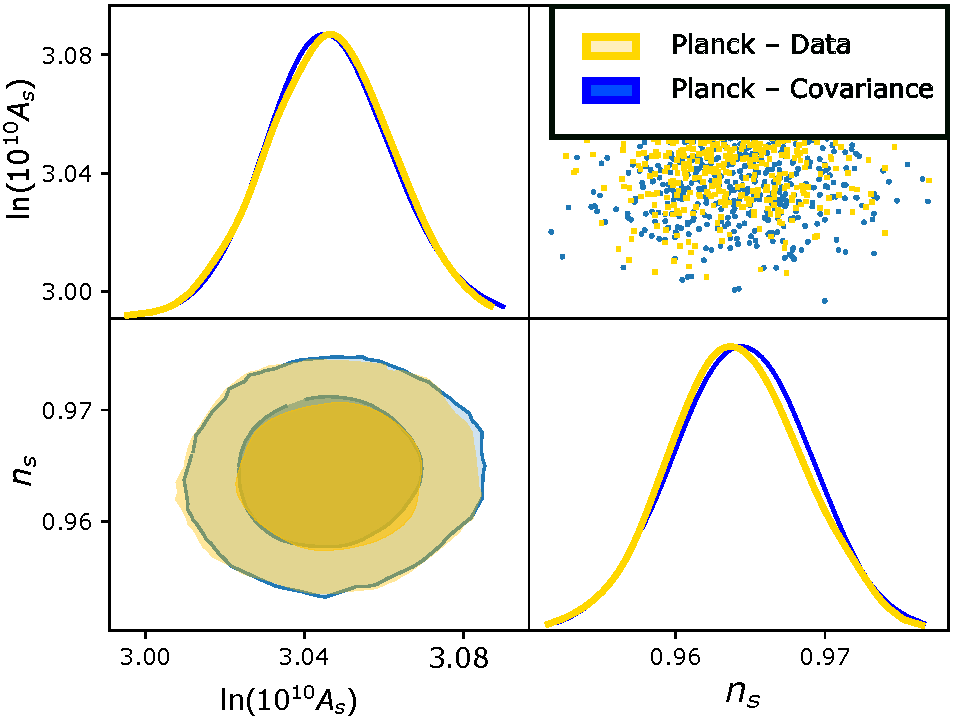
\includegraphics[width=0.5\textwidth]{./illustrations/triangle-fit.pdf}
  \caption{An example of a posterior obtained with PPR, based on
    Planck parameter covariance matrix, compared with the Planck
    posterior chains. The differences in the distributions indicate
    variance across different inference runs.
    ${\cal D}\{ {\cal P}, \bar{\cal P}\} \approx 0.01$. The deviation
    is due to a different (smaller) number of live points used, and
    the difference between the correct likelihood and its
    approximation using a Gaussian. \label{fig:overlay-posteriors}}
\end{figure}


\subsection{Simulations}
\subsubsection{Numerical models}

We shall begin our analysis with help of a simplified model that is
general-enough to share features with the Cosmological scale problem,
but also practical to investigate in depth, with multiple variations.

Our original model is a Gaussian peak. By choosing the uniform prior
as a baseline, and setting the log-likelihood as:
\begin{equation}
  \ln {\cal L}(\bm{\theta}) = - \dfrac{1}{2} \left\{{(\bm{\theta} - \bm{\mu})}^{T}G^{-1}(\bm{\theta}-\bm{\mu})  + \ln \det \left| 2\mathrm{\pi} \bm{\Sigma}\right| \right\},
\end{equation}
where the covariance matrix \(\bm{\Sigma}\), specifies the extent of
the peak, and the vector \(\bm{\mu}\), its location. We thus expect
the posterior to be a truncated and re-scaled Gaussian. However its
typical set is still approximately at a distance of the square root of
the diagonal elements of the covariance matrix form the peak,
i.e.~\emph{one standard deviation}.

The covariance matrix is positive semi-definite and symmetric, hence
it can be diagonalised \citep{taboga2017lectures}. If the covariance
matrix is diagonal, the Gaussian distribution is called
uncorrelated. If all diagonal elements are equal, then the Gaussian is
spherical with characteristic diameter given by
\(2\bm{\sigma} = 2\sqrt{\bm{\Sigma}}\), where \(\bm{\Sigma} = \Sigma \mathds{1}\).

To simulate imperfections we shall consider translation-al offsets
between the proposed prior and the likelihood.

\section{Results and Discussion.}\label{sec:results}
The first test case is an uncorrelated spherical Gaussian posterior
in three dimensions \[\mathcal{P}(\bm{\theta}) = G(\bm{\theta}; \bm{\mu} =
  (1,2,3),\bm{\sigma} = \mathds{1}).\] The corresponding evidence
(\cref{eq:evidence}) is \(\mathcal{Z}\approx-62.3\). First we shall
assume that the mean and standard deviation of all the
repartitioning schemes is exactly the same as that of the
posterior.

All but one repartitioning scheme yielded the correct evidence. The
resize-able uniform prior model was constructed to systematically
overestimating the evidence (\cref{fig:hist}) which is due to
underestimating the normalisation factor for
\(\mathcal{L}\).


We shall now show that repartitioning is able to drastically reduce
the run-time compared to using a uniform prior. More specifically,
proposing a posterior distribution and using repartitioning, one may
reduce the initial compression stage to virtually none.

Having proven the correctness of the runs, let's turn to performance
and benchmarks. The central metric is the number of \({\cal L}\)
evaluations. \cref{fig:benchmark} shows that mixture
repartitioning, produces a significant speed-up compared to even
power-posterior repartitioning. Moreover, the slope of the curve of
the number of \({\cal L}\) evaluations is much steeper for the
slower repartitioning schemes, indicating that for large numbers of
live points, mixture repartitioning yields an even greater
speed-up.



\begin{figure}
  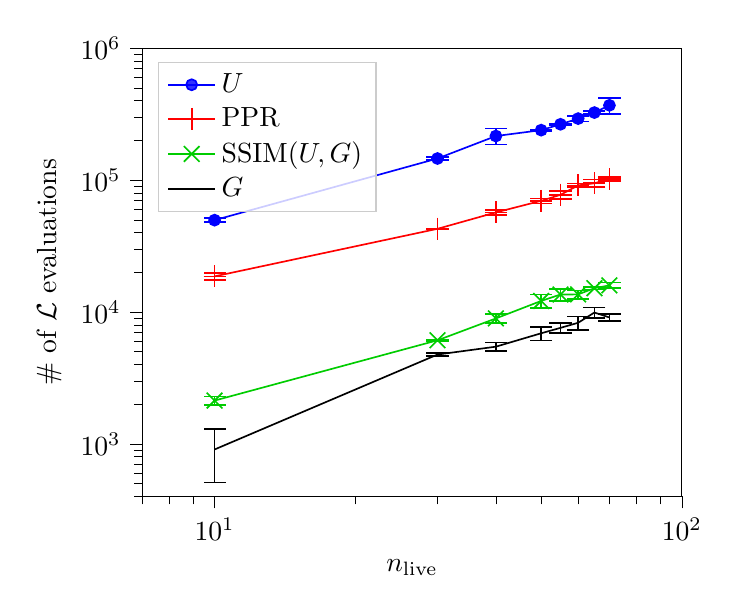
\begin{tikzpicture}

\definecolor{color0}{rgb}{0.0,0.0,1.0} %U
\definecolor{color1}{rgb}{1,0.0,0.0} %PPR
\definecolor{color2}{rgb}{0,0.8,0.0}                              %SSIM
\definecolor{color3}{rgb}{0.,0.0,0.0} %G

\begin{axis}[
legend cell align={left},
legend style={fill opacity=0.8, draw opacity=1, text opacity=1, at={(0.03,0.97)}, anchor=north west, draw=white!80!black},
tick align=outside,
tick pos=left,
x grid style={white!69.0196078431373!black},
xlabel={\(n_\text{live}\)},
xmin=7, xmax=100,
xtick style={color=black},
y grid style={white!69.0196078431373!black},
ylabel={\# of \({\cal L}\) evaluations},
ymin=400, ymax=1000000.0,
ytick style={color=black},
xmode=log,
ymode=log
]
\path [draw=color0, semithick]
(axis cs:10,48051.1762746562)
--(axis cs:10,51361.4903920105);

\path [draw=color0, semithick]
(axis cs:30,141787.579248368)
--(axis cs:30,149701.087418299);

\path [draw=color0, semithick]
(axis cs:40,185671.527674282)
--(axis cs:40,245784.472325718);

\path [draw=color0, semithick]
(axis cs:50,236296.832694899)
--(axis cs:50,241822.500638435);

\path [draw=color0, semithick]
(axis cs:55,262655.71356965)
--(axis cs:55,266952.953097016);

\path [draw=color0, semithick]
(axis cs:60,278243.015081106)
--(axis cs:60,306644.984918894);

\path [draw=color0, semithick]
(axis cs:65,317116.521541605)
--(axis cs:65,332736.145125062);

\path [draw=color0, semithick]
(axis cs:70,318358.948415036)
--(axis cs:70,419081.71825163);

\path [draw=color1, semithick]
(axis cs:10,17520.6487596482)
--(axis cs:10,19742.0179070185);

\path [draw=color1, semithick]
(axis cs:30,42472.9620658463)
--(axis cs:30,42994.371267487);

\path [draw=color1, semithick]
(axis cs:40,54281.6999405287)
--(axis cs:40,59494.3000594713);

\path [draw=color1, semithick]
(axis cs:50,66559.0160569084)
--(axis cs:50,72717.6506097582);

\path [draw=color1, semithick]
(axis cs:55,71552.6011973656)
--(axis cs:55,83118.7321359677);

\path [draw=color1, semithick]
(axis cs:60,88312.8386239607)
--(axis cs:60,94072.4947093726);

\path [draw=color1, semithick]
(axis cs:65,88215.9096228476)
--(axis cs:65,100992.090377152);

\path [draw=color1, semithick]
(axis cs:70,97882.04633)
--(axis cs:70,105637.95367);

\path [draw=color2, semithick]
(axis cs:10,1980.99743591911)
--(axis cs:10,2284.33589741422);

\path [draw=color2, semithick]
(axis cs:30,6035.87692136486)
--(axis cs:30,6174.12307863514);

\path [draw=color2, semithick]
(axis cs:40,8260.41435100755)
--(axis cs:40,9624.91898232578);

\path [draw=color2, semithick]
(axis cs:50,10733.0849396109)
--(axis cs:50,13538.9150603891);

\path [draw=color2, semithick]
(axis cs:55,12122.9645002052)
--(axis cs:55,15015.0354997948);

\path [draw=color2, semithick]
(axis cs:60,12622.7721075812)
--(axis cs:60,14593.2278924188);

\path [draw=color2, semithick]
(axis cs:65,14804.9685728395)
--(axis cs:65,15505.0314271605);

\path [draw=color2, semithick]
(axis cs:70,15158.1193669152)
--(axis cs:70,16693.8806330848);

\path [draw=color3, semithick]
(axis cs:10,511.628293172651)
--(axis cs:10,1305.03837349402);

\path [draw=color3, semithick]
(axis cs:30,4625.34584399058)
--(axis cs:30,4900.65415600942);

\path [draw=color3, semithick]
(axis cs:40,5045.39013421616)
--(axis cs:40,5880.60986578384);

\path [draw=color3, semithick]
(axis cs:50,6085.69651897324)
--(axis cs:50,7719.6368143601);

\path [draw=color3, semithick]
(axis cs:55,6959.0338647499)
--(axis cs:55,8215.63280191676);

\path [draw=color3, semithick]
(axis cs:60,7317.2571539732)
--(axis cs:60,9267.40951269347);

\path [draw=color3, semithick]
(axis cs:65,8986.02980736454)
--(axis cs:65,10838.6368593021);

\path [draw=color3, semithick]
(axis cs:70,8588.48027282128)
--(axis cs:70,9612.18639384539);


\addplot [semithick, color1, mark=-, mark size=4, mark options={solid}, only marks, forget plot]
table {%
10 17520.6487596482
30 42472.9620658463
40 54281.6999405287
50 66559.0160569084
55 71552.6011973656
60 88312.8386239607
65 88215.9096228476
70 97882.04633
};
\addplot [semithick, color1, mark=-, mark size=4, mark options={solid}, only marks, forget plot]
table {%
10 19742.0179070185
30 42994.371267487
40 59494.3000594713
50 72717.6506097582
55 83118.7321359677
60 94072.4947093726
65 100992.090377152
70 105637.95367
};
\addplot [semithick, color2, mark=-, mark size=4, mark options={solid}, only marks, forget plot]
table {%
10 1980.99743591911
30 6035.87692136486
40 8260.41435100755
50 10733.0849396109
55 12122.9645002052
60 12622.7721075812
65 14804.9685728395
70 15158.1193669152
};
\addplot [semithick, color2, mark=-, mark size=4, mark options={solid}, only marks, forget plot]
table {%
10 2284.33589741422
30 6174.12307863514
40 9624.91898232578
50 13538.9150603891
55 15015.0354997948
60 14593.2278924188
65 15505.0314271605
70 16693.8806330848
};
\addplot [semithick, color3, mark=-, mark size=4, mark options={solid}, only marks, forget plot]
table {%
10 511.628293172651
30 4625.34584399058
40 5045.39013421616
50 6085.69651897324
55 6959.0338647499
60 7317.2571539732
65 8986.02980736454
70 8588.48027282128
};
\addplot [semithick, color3, mark=-, mark size=4, mark options={solid}, only marks, forget plot]
table {%
10 1305.03837349402
30 4900.65415600942
40 5880.60986578384
50 7719.6368143601
55 8215.63280191676
60 9267.40951269347
65 10838.6368593021
70 9612.18639384539
};
\addplot [semithick, color0, mark=-, mark size=4, mark options={solid}, only marks, forget plot]
table {%
10 48051.1762746562
30 141787.579248368
40 185671.527674282
50 236296.832694899
55 262655.71356965
60 278243.015081106
65 317116.521541605
70 318358.948415036
};
\addplot [semithick, color0, mark=-, mark size=4, mark options={solid}, only marks, forget plot]
table {%
10 51361.4903920105
30 149701.087418299
40 245784.472325718
50 241822.500638435
55 266952.953097016
60 306644.984918894
65 332736.145125062
70 419081.71825163
};
\addplot [semithick, color0, mark=*, mark size=2, mark options={solid}]
table {%
10 49706.3333333333
30 145744.333333333
40 215728
50 239059.666666667
55 264804.333333333
60 292444
65 324926.333333333
70 368720.333333333
};
\addlegendentry{$U$}
\addplot [semithick, color1, mark=+, mark size=4, mark options={solid}]
table {%
10 18631.3333333333
30 42733.6666666667
40 56888
50 69638.3333333333
55 77335.6666666667
60 91192.6666666667
65 94604
70 101760
};
\addlegendentry{PPR}
\addplot [semithick, color2, mark=x, mark size=4, mark options={solid}]
table {%
10 2132.66666666667
30 6105
40 8942.66666666667
50 12136
55 13569
60 13608
65 15155
70 15926
};
\addlegendentry{$\text{SSIM}(U,G)$}
\addplot [semithick, color3, mark=., mark size=2, mark options={solid}]
table {%
10 908.333333333333
30 4763
40 5463
50 6902.66666666667
55 7587.33333333333
60 8292.33333333333
65 9912.33333333333
70 9100.33333333333
};
\addlegendentry{$G$}
\end{axis}

\end{tikzpicture}

  \caption{number of ${\cal L}$ evaluations as a function of the
    number of live points. From the slope of best-fit lines, the
    number of evaluations scales as $k\cdot n_\text{live}^{1.1 \pm 0.2}$,
    where $\kappa$ reduces across repartitioning
    schemes. \label{fig:benchmark}}
\end{figure}


The next trial involved a variable offset, where convergence to the
correct posterior and evidence is not guaranteed even with the correct
normalisation. For this case, we have taken the same Gaussian
truncated to a cube \(1000\times1000\times1000\). Two types of
sampling runs were considered: one where the posterior and prior
distributions coincided, and one with the mean of the posterior
shifted relative to the prior by an amount proportional to the mean
$\mu = (1,2,3)$.

The exemplary results are given in \cref{fig:convergence}. The main
notable feature is the inaccuracy of the posterior for PPR. If the
offset is small --- \(O(2\sigma)\), the posterior is shifted. With a
larger offset, e.g. \(O(4\sigma)\), two peaks can be resolved, sadly,
with less density near the correct Gaussian peak. Both errors are
compounded by incorrect evidence (see \cref{fig:drift}) PPR:
\(\ln {\cal Z}\approx -25.4 \pm 0.2\), vs uniform reference
\(\ln {\cal Z} = -22.7 \pm 0.4\).

In practice one has the following options:
\begin{enumerate}
\item accept the posterior as is~\label[Option]{opt:accept}
\item accept the posterior, but as a less credible result\label[Option]{opt:accept-with-err}
\item reject the PPR result entirely, and perform a run with only a
uniform prior\label[Option]{opt:uniform}
\item readjust the PPR mean and variance using the posterior, and
re-run~\label[Option]{opt:shift}
\item combine PPR with SSIM in mixture with a uniform prior
\end{enumerate}
\vref{opt:accept} is adequate for low accuracy standards provided the
error is properly estimated using a tool such as \texttt{nestcheck}.
From \cref{fig:benchmark}, we see that the performance uplift allows
for \cref{opt:shift} to be more efficient than~\ref{opt:uniform},
albeit marginally so. \Cref{opt:accept-with-err} is a last resort.

This is where our technique is most useful: one obtains, as we've
shown in~\cref{fig:convergence}, a more accurate
\({\cal P}(\bm{\theta})\), by using PPR from within SSIM. The
performance impact has considerable run-to-run variance, however never
exceeds \(20\%\) extra \({\cal L}\) evaluations, which is an order of
magnitude less than~\vref{opt:uniform,opt:shift} would afford.

\begin{figure}
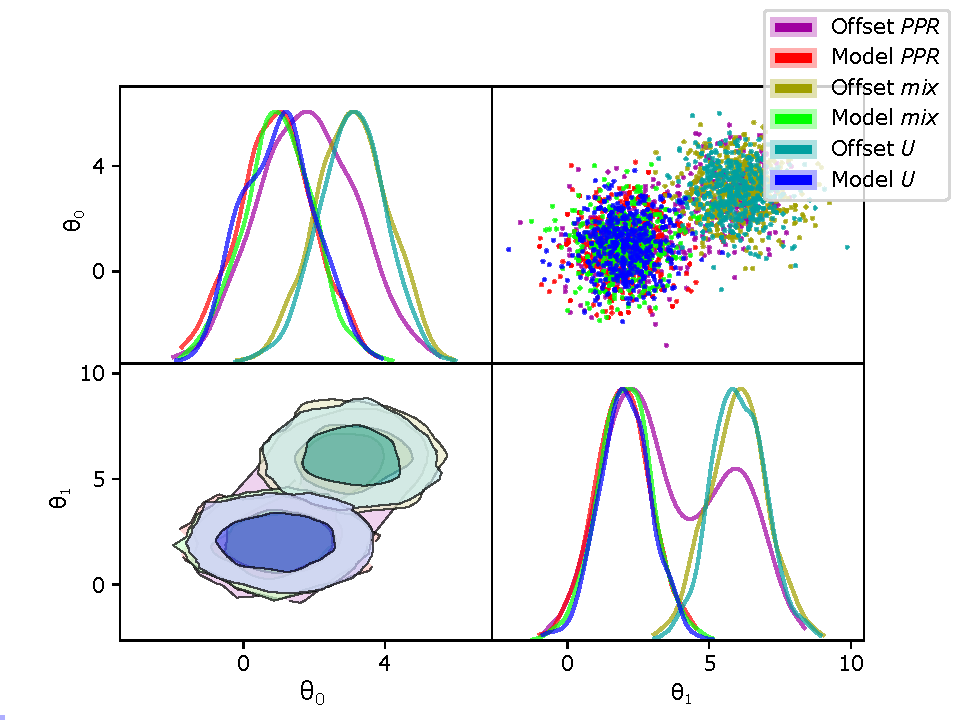
\includegraphics[width=0.5\textwidth]{./illustrations/convergence.pdf}
\caption{An illustration of offsets affecting ${\cal P}$ under various
  repartitioning schemes. Dotted series represent the prior
  bias. \label{fig:convergence}}
\end{figure}

\begin{figure} \centering
  \begin{subfigure}{0.86\columnwidth}
    \centering

    % This file was created by tikzplotlib v0.9.1.
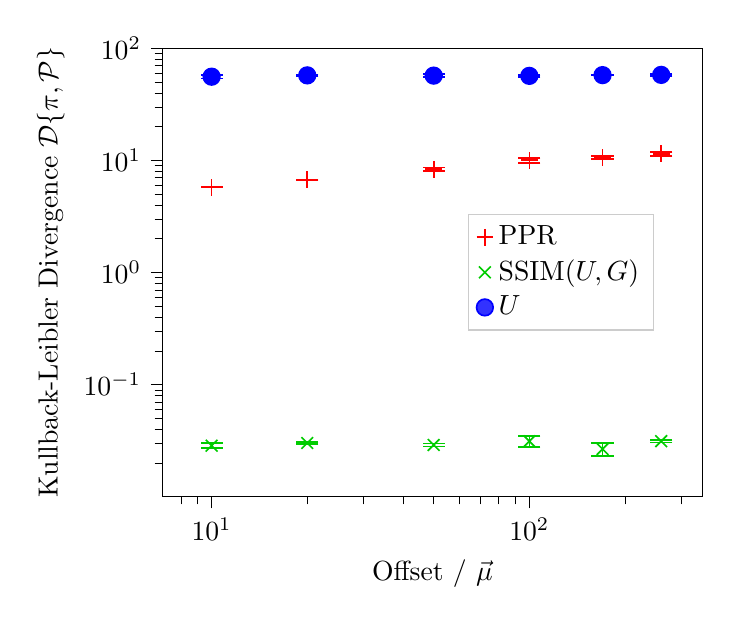
\begin{tikzpicture}

\definecolor{color0}{rgb}{1,0.0,0.0} %ppr
\definecolor{color1}{rgb}{0,0.8,0.0} %mix
\definecolor{color2}{rgb}{0.0,0.0,1.0} %U

\begin{axis}[
legend cell align={left},
legend style={fill opacity=0.8, draw opacity=1, text opacity=1, at={(0.91,0.5)}, anchor=east, draw=white!80!black},
tick align=outside,
tick pos=left,
x grid style={white!69.0196078431373!black},
xlabel={Offset / \(\displaystyle \vec{\mu}\)},
xmin=-3.0, xmax=350.0,
xtick style={color=black},
y grid style={white!69.0196078431373!black},
ylabel={Kullback-Leibler Divergence \(\displaystyle {\cal D}\{\pi, {\cal P}\}\)},
ymin=-3.0, ymax=100.0,
ytick style={color=black},
xmode=log,
ymode=log
]
\path [draw=color0, semithick]
(axis cs:10,5.71795365099151)
--(axis cs:10,5.77133948534581);

\path [draw=color0, semithick]
(axis cs:20,6.6768824419002)
--(axis cs:20,6.77321107556694);

\path [draw=color0, semithick]
(axis cs:50,8.02877279045042)
--(axis cs:50,8.63543918622054);

\path [draw=color0, semithick]
(axis cs:100,9.52185212376919)
--(axis cs:100,10.4908349952443);

\path [draw=color0, semithick]
(axis cs:170,10.3029683750536)
--(axis cs:170,10.9155451202318);

\path [draw=color0, semithick]
(axis cs:260,10.954510866509)
--(axis cs:260,11.9335782130671);

\path [draw=color1, semithick]
(axis cs:10,0.0271909650803472)
--(axis cs:10,0.030089733601838);

\path [draw=color1, semithick]
(axis cs:20,0.029683008672791)
--(axis cs:20,0.0308036500189849);

\path [draw=color1, semithick]
(axis cs:50,0.0282101242046804)
--(axis cs:50,0.0298855157628486);

\path [draw=color1, semithick]
(axis cs:100,0.0278177027329167)
--(axis cs:100,0.0348526563256524);

\path [draw=color1, semithick]
(axis cs:170,0.0232802581598788)
--(axis cs:170,0.0301604324600733);

\path [draw=color1, semithick]
(axis cs:260,0.0304771056975755)
--(axis cs:260,0.0323746358923458);

\path [draw=color2, semithick]
(axis cs:10,53.6407046096139)
--(axis cs:10,57.7293889288474);

\path [draw=color2, semithick]
(axis cs:20,56.1280894679801)
--(axis cs:20,58.3022565457241);

\path [draw=color2, semithick]
(axis cs:50,55.3633380690649)
--(axis cs:50,58.47445725549);

\path [draw=color2, semithick]
(axis cs:100,55.5223746731559)
--(axis cs:100,57.7271641567295);

\path [draw=color2, semithick]
(axis cs:170,56.8924880373743)
--(axis cs:170,58.1261131182599);

\path [draw=color2, semithick]
(axis cs:260,56.3603430284318)
--(axis cs:260,59.2024246504929);

\addplot [semithick, color0, mark=-, mark size=4, mark options={solid}, only marks, forget plot]
table {%
10 5.71795365099151
20 6.6768824419002
50 8.02877279045042
100 9.52185212376919
170 10.3029683750536
260 10.954510866509
};
\addplot [semithick, color0, mark=-, mark size=4, mark options={solid}, only marks, forget plot]
table {%
10 5.77133948534581
20 6.77321107556694
50 8.63543918622054
100 10.4908349952443
170 10.9155451202318
260 11.9335782130671
};
\addplot [semithick, color1, mark=-, mark size=4, mark options={solid}, only marks, forget plot]
table {%
10 0.0271909650803472
20 0.029683008672791
50 0.0282101242046804
100 0.0278177027329167
170 0.0232802581598788
260 0.0304771056975755
};
\addplot [semithick, color1, mark=-, mark size=4, mark options={solid}, only marks, forget plot]
table {%
10 0.030089733601838
20 0.0308036500189849
50 0.0298855157628486
100 0.0348526563256524
170 0.0301604324600733
260 0.0323746358923458
};
\addplot [semithick, color2, mark=-, mark size=4, mark options={solid}, only marks, forget plot]
table {%
10 53.6407046096139
20 56.1280894679801
50 55.3633380690649
100 55.5223746731559
170 56.8924880373743
260 56.3603430284318
};
\addplot [semithick, color2, mark=-, mark size=4, mark options={solid}, only marks, forget plot]
table {%
10 57.7293889288474
20 58.3022565457241
50 58.47445725549
100 57.7271641567295
170 58.1261131182599
260 59.2024246504929
};
\addplot [semithick, color0, mark=+, mark size=3, mark options={solid}, only marks]
table {%
10 5.74464656816866
20 6.72504675873357
50 8.33210598833548
100 10.0063435595067
170 10.6092567476427
260 11.4440445397881
};
\addlegendentry{PPR}
\addplot [semithick, color1, mark=x, mark size=3, mark options={solid}, only marks]
table {%
10 0.0286403493410926
20 0.0302433293458879
50 0.0290478199837645
100 0.0313351795292845
170 0.026720345309976
260 0.0314258707949607
};
\addlegendentry{SSIM$(U,G)$}
\addplot [semithick, color2, mark=*, mark size=3, mark options={solid}, only marks]
table {%
10 55.6850467692306
20 57.2151730068521
50 56.9188976622774
100 56.6247694149427
170 57.5093005778171
260 57.7813838394624
};
\addlegendentry{$U$}
\end{axis}

\end{tikzpicture}

    \caption{Kullback-Leibler divergence \({\cal D}\) for different
      offsets: Gaussian peaks displaced from \(\bm{\mu}\) by
      \(\text{Offset}\times \bm{\mu}\). Notice that the faster
      repartitioning methods produce a lower value of \({\cal
        D}\). The divergence \({\cal D}\) scales sub-linearly with the
      offset.\label{fig:kl-d}}
\end{subfigure}

\begin{subfigure}{0.86\columnwidth}
  \centering

  % This file was created by tikzplotlib v0.9.1.
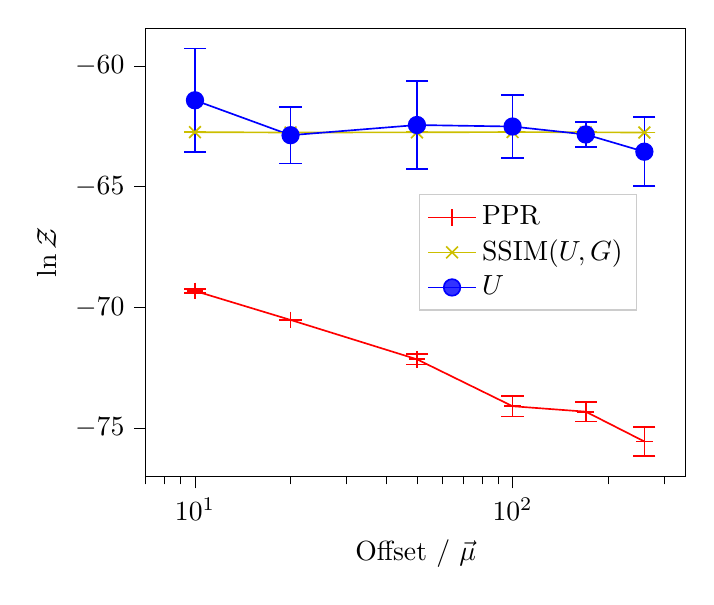
\begin{tikzpicture}

\definecolor{color0}{rgb}{1,0.0,0.0}
\definecolor{color1}{rgb}{0.8,0.75,0.0}
\definecolor{color2}{rgb}{0.0,0.0,1}

\begin{axis}[
legend cell align={left},
legend style={fill opacity=0.8, draw opacity=1, text opacity=1, at={(0.91,0.5)}, anchor=east, draw=white!80!black},
tick align=outside,
tick pos=left,
x grid style={white!69.0196078431373!black},
xlabel={Offset / \(\displaystyle \vec{\mu}\)},
xmin=-2.5, xmax=350.5,
xtick style={color=black},
y grid style={white!69.0196078431373!black},
ylabel={\(\displaystyle \ln {\cal Z}\)},
ymin=-77.013439988999, ymax=-58.4325947574349,
ytick style={color=black},
xmode=log
]
\path [draw=color0, semithick]
(axis cs:10,-69.4059960469118)
--(axis cs:10,-69.2379297037398);

\path [draw=color0, semithick]
(axis cs:20,-70.5299156173721)
--(axis cs:20,-70.5157474991409);

\path [draw=color0, semithick]
(axis cs:50,-72.3755951664078)
--(axis cs:50,-71.9328145858461);

\path [draw=color0, semithick]
(axis cs:100,-74.5305277482911)
--(axis cs:100,-73.6673769114354);

\path [draw=color0, semithick]
(axis cs:170,-74.7380053024013)
--(axis cs:170,-73.9121550603194);

\path [draw=color0, semithick]
(axis cs:260,-76.168856114837)
--(axis cs:260,-74.9518470928008);

\path [draw=color1, semithick]
(axis cs:10,-62.7439928102151)
--(axis cs:10,-62.7359696372663);

\path [draw=color1, semithick]
(axis cs:20,-62.755485458383)
--(axis cs:20,-62.7535773275597);

\path [draw=color1, semithick]
(axis cs:50,-62.7484141957878)
--(axis cs:50,-62.7468638775576);

\path [draw=color1, semithick]
(axis cs:100,-62.7369486572665)
--(axis cs:100,-62.7333125352419);

\path [draw=color1, semithick]
(axis cs:170,-62.746863877575)
--(axis cs:170,-62.745391448683);

\path [draw=color1, semithick]
(axis cs:260,-62.7574960930232)
--(axis cs:260,-62.7517661617973);

\path [draw=color2, semithick]
(axis cs:10,-63.5623386499016)
--(axis cs:10,-59.2771786315969);

\path [draw=color2, semithick]
(axis cs:20,-64.0348662974579)
--(axis cs:20,-61.6973543628668);

\path [draw=color2, semithick]
(axis cs:50,-64.2749108611421)
--(axis cs:50,-60.6135450768888);

\path [draw=color2, semithick]
(axis cs:100,-63.8144479355573)
--(axis cs:100,-61.1997313352197);

\path [draw=color2, semithick]
(axis cs:170,-63.3536082125541)
--(axis cs:170,-62.3180044247467);

\path [draw=color2, semithick]
(axis cs:260,-64.9781441262723)
--(axis cs:260,-62.1236339929356);

\addplot [semithick, color0, mark=-, mark size=4, mark options={solid}, only marks, forget plot]
table {%
10 -69.4059960469118
20 -70.5299156173721
50 -72.3755951664078
100 -74.5305277482911
170 -74.7380053024013
260 -76.168856114837
};
\addplot [semithick, color0, mark=-, mark size=4, mark options={solid}, only marks, forget plot]
table {%
10 -69.2379297037398
20 -70.5157474991409
50 -71.9328145858461
100 -73.6673769114354
170 -73.9121550603194
260 -74.9518470928008
};
\addplot [semithick, color1, mark=-, mark size=4, mark options={solid}, only marks, forget plot]
table {%
10 -62.7439928102151
20 -62.755485458383
50 -62.7484141957878
100 -62.7369486572665
170 -62.746863877575
260 -62.7574960930232
};
\addplot [semithick, color1, mark=-, mark size=4, mark options={solid}, only marks, forget plot]
table {%
10 -62.7359696372663
20 -62.7535773275597
50 -62.7468638775576
100 -62.7333125352419
170 -62.745391448683
260 -62.7517661617973
};
\addplot [semithick, color2, mark=-, mark size=4, mark options={solid}, only marks, forget plot]
table {%
10 -63.5623386499016
20 -64.0348662974579
50 -64.2749108611421
100 -63.8144479355573
170 -63.3536082125541
260 -64.9781441262723
};
\addplot [semithick, color2, mark=-, mark size=4, mark options={solid}, only marks, forget plot]
table {%
10 -59.2771786315969
20 -61.6973543628668
50 -60.6135450768888
100 -61.1997313352197
170 -62.3180044247467
260 -62.1236339929356
};
\addplot [semithick, color0, mark=+, mark size=3, mark options={solid}]
table {%
10 -69.3219628753258
20 -70.5228315582565
50 -72.154204876127
100 -74.0989523298633
170 -74.3250801813604
260 -75.5603516038189
};
\addlegendentry{PPR}
\addplot [semithick, color1, mark=x, mark size=3, mark options={solid}]
table {%
10 -62.7399812237407
20 -62.7545313929713
50 -62.7476390366727
100 -62.7351305962542
170 -62.746127663129
260 -62.7546311274102
};
\addlegendentry{SSIM$(U, G)$}
\addplot [semithick, color2, mark=*, mark size=3, mark options={solid}]
table {%
10 -61.4197586407493
20 -62.8661103301623
50 -62.4442279690155
100 -62.5070896353885
170 -62.8358063186504
260 -63.5508890596039
};
\addlegendentry{$U$}
\end{axis}

\end{tikzpicture}

  
  \caption{An illustration of offsets affecting ${\cal Z}$. The true
    value is constant, mirrored by the mixture: SSIM of PPR and
    reference uniform. PPR alone produces incorrect evidence,
    consistent with \cref{fig:convergence}. \label{fig:drift}}
\end{subfigure}
\caption{Illustrations of effects of offsets on the correctness
  \ref{fig:drift} and performance \ref{fig:kl-d} of nested sampling
  under consistent posterior repartitioning.}
:\end{figure}



Lastly, \emph{posterior mass} is a measure of converge
speed~\cite{higson2018nestcheck}, often used in diagnosing nested
sampling. Typical examples of posterior mass for a run with
$\pi=\text{Const.}$ and runs accelerated by posterior repartitioning
are given in \cref{fig:higson}. Notice that the repartitioned series
has a longer extinction phase, as a result of introducing extra
nuisance parameters. Also, the confidence intervals on each parameter
between the uniform and the repartitioned run are identical,
signifying that we have not lost precision.

\begin{figure*}
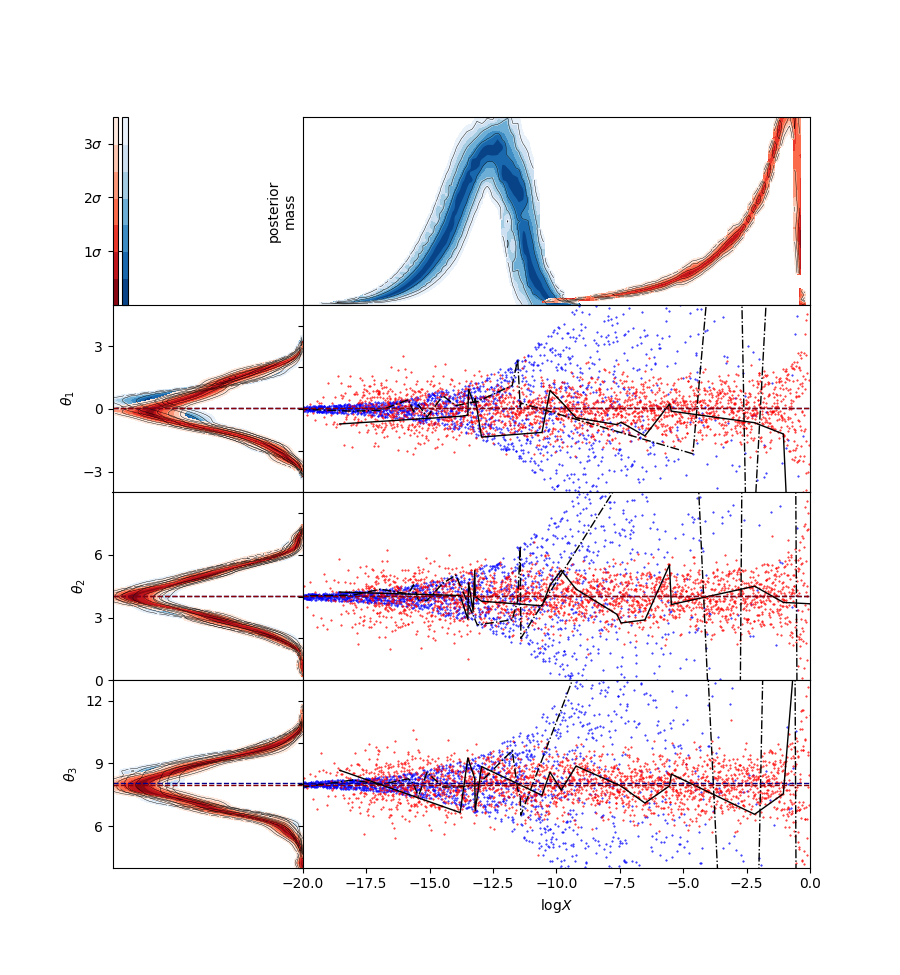
\includegraphics[width=.9\textwidth]{./illustrations/higson.png}
\caption{plot of the evolution of nested sampling. The \color{red} red
  \color{black} series corresponds to SSIM of iPPR, while the
  \color{blue} blue \color{black} series --- to a reference
  uniform. The horizontal axis of plots in the second column is
  \(\ln X\), where \(X(\mathcal{L}) \in [0,1]\) is the fraction of the
  prior with likelihood greater than \(\mathcal{L}\). The top plot is
  the relative posterior mass. In row $i$ the ${\cal P}(\theta_{i})$
  is plotted. Confidence intervals represented with color
  intensity. \label{fig:higson}}
\end{figure*}




\subsection{Cosmological Simulations.}\label{sec:orgb81c159}
After an initial run of \texttt{Cobaya}, we have obtained the marginalised
posteriors of all the key parameters of the \(\Lambda\)CDM model,
as well as the nuisance parameters.

First, we have performed an inference using the~\cite{Planck} dataset,
with the \(\Lambda\)CDM model. The results of our initial run are
presented in \cref{fig:cosmology}. From these data, under the
assumption that the parameters' posteriors are a correlated Gaussian
distribution, we extract the means $\bm{\mu}$ and the covariance
matrix \(\bm{\Sigma}\).

We use these in a stochastic superpositional mixture of a uniform
$\pi$ used to obtain them originally and a Gaussian iPPR, patched into
\texttt{Cobaya}'s interface to \texttt{PolyChord}. The run was then
performed with identical settings, and the resulting posteriors were
compared: ${\cal D}\{ {\cal P}, \bar{\cal P}\}$ and ${\cal Z}$,
alongside the marginalised posterior plots \cref{fig:cosmology-cmp}. 
\begin{landscape}
\begin{figure}
  \centering % Center table
  %% Creator: Matplotlib, PGF backend
%%
%% To include the figure in your LaTeX document, write
%%   \input{<filename>.pgf}
%%
%% Make sure the required packages are loaded in your preamble
%%   \usepackage{pgf}
%%
%% and, on pdftex
%%   \usepackage[utf8]{inputenc}\DeclareUnicodeCharacter{2212}{-}
%%
%% or, on luatex and xetex
%%   \usepackage{unicode-math}
%%
%% Figures using additional raster images can only be included by \input if
%% they are in the same directory as the main LaTeX file. For loading figures
%% from other directories you can use the `import` package
%%   \usepackage{import}
%%
%% and then include the figures with
%%   \import{<path to file>}{<filename>.pgf}
%%
%% Matplotlib used the following preamble
%%   \usepackage{fontspec}
%%   \setmainfont{DejaVuSerif.ttf}[Path=/usr/local/lib/python3.7/site-packages/matplotlib/mpl-data/fonts/ttf/]
%%   \setsansfont{DejaVuSans.ttf}[Path=/usr/local/lib/python3.7/site-packages/matplotlib/mpl-data/fonts/ttf/]
%%   \setmonofont{DejaVuSansMono.ttf}[Path=/usr/local/lib/python3.7/site-packages/matplotlib/mpl-data/fonts/ttf/]
%%
\begingroup%
\makeatletter%
\begin{pgfpicture}%
\pgfpathrectangle{\pgfpointorigin}{\pgfqpoint{7.750000in}{5.070000in}}%
\pgfusepath{use as bounding box, clip}%
\begin{pgfscope}%
\pgfsetbuttcap%
\pgfsetmiterjoin%
\definecolor{currentfill}{rgb}{1.000000,1.000000,1.000000}%
\pgfsetfillcolor{currentfill}%
\pgfsetlinewidth{0.000000pt}%
\definecolor{currentstroke}{rgb}{1.000000,1.000000,1.000000}%
\pgfsetstrokecolor{currentstroke}%
\pgfsetdash{}{0pt}%
\pgfpathmoveto{\pgfqpoint{0.000000in}{0.000000in}}%
\pgfpathlineto{\pgfqpoint{7.750000in}{0.000000in}}%
\pgfpathlineto{\pgfqpoint{7.750000in}{5.070000in}}%
\pgfpathlineto{\pgfqpoint{0.000000in}{5.070000in}}%
\pgfpathclose%
\pgfusepath{fill}%
\end{pgfscope}%
\begin{pgfscope}%
\pgfsetbuttcap%
\pgfsetmiterjoin%
\definecolor{currentfill}{rgb}{1.000000,1.000000,1.000000}%
\pgfsetfillcolor{currentfill}%
\pgfsetlinewidth{0.000000pt}%
\definecolor{currentstroke}{rgb}{0.000000,0.000000,0.000000}%
\pgfsetstrokecolor{currentstroke}%
\pgfsetstrokeopacity{0.000000}%
\pgfsetdash{}{0pt}%
\pgfpathmoveto{\pgfqpoint{0.711624in}{0.446542in}}%
\pgfpathlineto{\pgfqpoint{1.862862in}{0.446542in}}%
\pgfpathlineto{\pgfqpoint{1.862862in}{1.197618in}}%
\pgfpathlineto{\pgfqpoint{0.711624in}{1.197618in}}%
\pgfpathclose%
\pgfusepath{fill}%
\end{pgfscope}%
\begin{pgfscope}%
\pgfpathrectangle{\pgfqpoint{0.711624in}{0.446542in}}{\pgfqpoint{1.151239in}{0.751076in}}%
\pgfusepath{clip}%
\pgfsetbuttcap%
\pgfsetroundjoin%
\definecolor{currentfill}{rgb}{0.600000,0.774118,0.971765}%
\pgfsetfillcolor{currentfill}%
\pgfsetlinewidth{0.000000pt}%
\definecolor{currentstroke}{rgb}{0.000000,0.000000,0.000000}%
\pgfsetstrokecolor{currentstroke}%
\pgfsetdash{}{0pt}%
\pgfpathmoveto{\pgfqpoint{0.927130in}{0.585816in}}%
\pgfpathlineto{\pgfqpoint{0.933743in}{0.584680in}}%
\pgfpathlineto{\pgfqpoint{0.940357in}{0.584557in}}%
\pgfpathlineto{\pgfqpoint{0.946971in}{0.584972in}}%
\pgfpathlineto{\pgfqpoint{0.953584in}{0.585611in}}%
\pgfpathlineto{\pgfqpoint{0.959551in}{0.586562in}}%
\pgfpathlineto{\pgfqpoint{0.960198in}{0.586660in}}%
\pgfpathlineto{\pgfqpoint{0.966811in}{0.587801in}}%
\pgfpathlineto{\pgfqpoint{0.973425in}{0.588954in}}%
\pgfpathlineto{\pgfqpoint{0.980038in}{0.590081in}}%
\pgfpathlineto{\pgfqpoint{0.983222in}{0.590704in}}%
\pgfpathlineto{\pgfqpoint{0.986652in}{0.591341in}}%
\pgfpathlineto{\pgfqpoint{0.993265in}{0.592562in}}%
\pgfpathlineto{\pgfqpoint{0.999879in}{0.593562in}}%
\pgfpathlineto{\pgfqpoint{1.006492in}{0.594732in}}%
\pgfpathlineto{\pgfqpoint{1.007144in}{0.594846in}}%
\pgfpathlineto{\pgfqpoint{1.013106in}{0.595816in}}%
\pgfpathlineto{\pgfqpoint{1.019719in}{0.596786in}}%
\pgfpathlineto{\pgfqpoint{1.026333in}{0.597723in}}%
\pgfpathlineto{\pgfqpoint{1.032947in}{0.598659in}}%
\pgfpathlineto{\pgfqpoint{1.035845in}{0.598988in}}%
\pgfpathlineto{\pgfqpoint{1.039560in}{0.599381in}}%
\pgfpathlineto{\pgfqpoint{1.046174in}{0.600072in}}%
\pgfpathlineto{\pgfqpoint{1.052787in}{0.600804in}}%
\pgfpathlineto{\pgfqpoint{1.059401in}{0.601599in}}%
\pgfpathlineto{\pgfqpoint{1.066014in}{0.602498in}}%
\pgfpathlineto{\pgfqpoint{1.070584in}{0.603130in}}%
\pgfpathlineto{\pgfqpoint{1.072628in}{0.603378in}}%
\pgfpathlineto{\pgfqpoint{1.079241in}{0.604329in}}%
\pgfpathlineto{\pgfqpoint{1.085855in}{0.605511in}}%
\pgfpathlineto{\pgfqpoint{1.092468in}{0.607097in}}%
\pgfpathlineto{\pgfqpoint{1.093089in}{0.607273in}}%
\pgfpathlineto{\pgfqpoint{1.099082in}{0.608896in}}%
\pgfpathlineto{\pgfqpoint{1.105695in}{0.610908in}}%
\pgfpathlineto{\pgfqpoint{1.107109in}{0.611415in}}%
\pgfpathlineto{\pgfqpoint{1.112309in}{0.613040in}}%
\pgfpathlineto{\pgfqpoint{1.118923in}{0.615379in}}%
\pgfpathlineto{\pgfqpoint{1.119385in}{0.615557in}}%
\pgfpathlineto{\pgfqpoint{1.125536in}{0.617825in}}%
\pgfpathlineto{\pgfqpoint{1.129944in}{0.619699in}}%
\pgfpathlineto{\pgfqpoint{1.132150in}{0.620591in}}%
\pgfpathlineto{\pgfqpoint{1.138763in}{0.623399in}}%
\pgfpathlineto{\pgfqpoint{1.139713in}{0.623841in}}%
\pgfpathlineto{\pgfqpoint{1.145377in}{0.626350in}}%
\pgfpathlineto{\pgfqpoint{1.148783in}{0.627983in}}%
\pgfpathlineto{\pgfqpoint{1.151990in}{0.629420in}}%
\pgfpathlineto{\pgfqpoint{1.157589in}{0.632125in}}%
\pgfpathlineto{\pgfqpoint{1.158604in}{0.632577in}}%
\pgfpathlineto{\pgfqpoint{1.165217in}{0.635723in}}%
\pgfpathlineto{\pgfqpoint{1.166298in}{0.636267in}}%
\pgfpathlineto{\pgfqpoint{1.171831in}{0.638953in}}%
\pgfpathlineto{\pgfqpoint{1.174650in}{0.640409in}}%
\pgfpathlineto{\pgfqpoint{1.178444in}{0.642272in}}%
\pgfpathlineto{\pgfqpoint{1.182841in}{0.644551in}}%
\pgfpathlineto{\pgfqpoint{1.185058in}{0.645655in}}%
\pgfpathlineto{\pgfqpoint{1.190835in}{0.648693in}}%
\pgfpathlineto{\pgfqpoint{1.191671in}{0.649124in}}%
\pgfpathlineto{\pgfqpoint{1.198285in}{0.652665in}}%
\pgfpathlineto{\pgfqpoint{1.198595in}{0.652835in}}%
\pgfpathlineto{\pgfqpoint{1.204899in}{0.656125in}}%
\pgfpathlineto{\pgfqpoint{1.206468in}{0.656977in}}%
\pgfpathlineto{\pgfqpoint{1.211512in}{0.659674in}}%
\pgfpathlineto{\pgfqpoint{1.214113in}{0.661119in}}%
\pgfpathlineto{\pgfqpoint{1.218126in}{0.663207in}}%
\pgfpathlineto{\pgfqpoint{1.221967in}{0.665261in}}%
\pgfpathlineto{\pgfqpoint{1.224739in}{0.666723in}}%
\pgfpathlineto{\pgfqpoint{1.229699in}{0.669403in}}%
\pgfpathlineto{\pgfqpoint{1.231353in}{0.670264in}}%
\pgfpathlineto{\pgfqpoint{1.237334in}{0.673545in}}%
\pgfpathlineto{\pgfqpoint{1.237966in}{0.673885in}}%
\pgfpathlineto{\pgfqpoint{1.244580in}{0.677576in}}%
\pgfpathlineto{\pgfqpoint{1.244773in}{0.677688in}}%
\pgfpathlineto{\pgfqpoint{1.251193in}{0.681249in}}%
\pgfpathlineto{\pgfqpoint{1.252237in}{0.681830in}}%
\pgfpathlineto{\pgfqpoint{1.257807in}{0.684783in}}%
\pgfpathlineto{\pgfqpoint{1.259962in}{0.685972in}}%
\pgfpathlineto{\pgfqpoint{1.264420in}{0.688430in}}%
\pgfpathlineto{\pgfqpoint{1.267383in}{0.690114in}}%
\pgfpathlineto{\pgfqpoint{1.271034in}{0.692108in}}%
\pgfpathlineto{\pgfqpoint{1.274823in}{0.694256in}}%
\pgfpathlineto{\pgfqpoint{1.277647in}{0.695790in}}%
\pgfpathlineto{\pgfqpoint{1.282268in}{0.698398in}}%
\pgfpathlineto{\pgfqpoint{1.284261in}{0.699523in}}%
\pgfpathlineto{\pgfqpoint{1.289446in}{0.702540in}}%
\pgfpathlineto{\pgfqpoint{1.290875in}{0.703342in}}%
\pgfpathlineto{\pgfqpoint{1.296574in}{0.706682in}}%
\pgfpathlineto{\pgfqpoint{1.297488in}{0.707212in}}%
\pgfpathlineto{\pgfqpoint{1.303642in}{0.710824in}}%
\pgfpathlineto{\pgfqpoint{1.304102in}{0.711091in}}%
\pgfpathlineto{\pgfqpoint{1.310560in}{0.714966in}}%
\pgfpathlineto{\pgfqpoint{1.310715in}{0.715057in}}%
\pgfpathlineto{\pgfqpoint{1.317329in}{0.719055in}}%
\pgfpathlineto{\pgfqpoint{1.317417in}{0.719108in}}%
\pgfpathlineto{\pgfqpoint{1.323942in}{0.723078in}}%
\pgfpathlineto{\pgfqpoint{1.324221in}{0.723250in}}%
\pgfpathlineto{\pgfqpoint{1.330556in}{0.727037in}}%
\pgfpathlineto{\pgfqpoint{1.331133in}{0.727392in}}%
\pgfpathlineto{\pgfqpoint{1.337169in}{0.731077in}}%
\pgfpathlineto{\pgfqpoint{1.337901in}{0.731534in}}%
\pgfpathlineto{\pgfqpoint{1.343783in}{0.735255in}}%
\pgfpathlineto{\pgfqpoint{1.344437in}{0.735676in}}%
\pgfpathlineto{\pgfqpoint{1.350396in}{0.739482in}}%
\pgfpathlineto{\pgfqpoint{1.350916in}{0.739818in}}%
\pgfpathlineto{\pgfqpoint{1.357010in}{0.743824in}}%
\pgfpathlineto{\pgfqpoint{1.357224in}{0.743961in}}%
\pgfpathlineto{\pgfqpoint{1.363623in}{0.748015in}}%
\pgfpathlineto{\pgfqpoint{1.363760in}{0.748103in}}%
\pgfpathlineto{\pgfqpoint{1.370167in}{0.752245in}}%
\pgfpathlineto{\pgfqpoint{1.370237in}{0.752289in}}%
\pgfpathlineto{\pgfqpoint{1.376678in}{0.756387in}}%
\pgfpathlineto{\pgfqpoint{1.376851in}{0.756498in}}%
\pgfpathlineto{\pgfqpoint{1.383040in}{0.760529in}}%
\pgfpathlineto{\pgfqpoint{1.383464in}{0.760810in}}%
\pgfpathlineto{\pgfqpoint{1.389283in}{0.764671in}}%
\pgfpathlineto{\pgfqpoint{1.390078in}{0.765204in}}%
\pgfpathlineto{\pgfqpoint{1.395470in}{0.768813in}}%
\pgfpathlineto{\pgfqpoint{1.396691in}{0.769647in}}%
\pgfpathlineto{\pgfqpoint{1.401576in}{0.772955in}}%
\pgfpathlineto{\pgfqpoint{1.403305in}{0.774169in}}%
\pgfpathlineto{\pgfqpoint{1.407524in}{0.777097in}}%
\pgfpathlineto{\pgfqpoint{1.409918in}{0.778759in}}%
\pgfpathlineto{\pgfqpoint{1.413537in}{0.781239in}}%
\pgfpathlineto{\pgfqpoint{1.416532in}{0.783349in}}%
\pgfpathlineto{\pgfqpoint{1.419460in}{0.785381in}}%
\pgfpathlineto{\pgfqpoint{1.423145in}{0.788029in}}%
\pgfpathlineto{\pgfqpoint{1.425281in}{0.789523in}}%
\pgfpathlineto{\pgfqpoint{1.429759in}{0.792733in}}%
\pgfpathlineto{\pgfqpoint{1.431083in}{0.793665in}}%
\pgfpathlineto{\pgfqpoint{1.436372in}{0.797533in}}%
\pgfpathlineto{\pgfqpoint{1.436759in}{0.797807in}}%
\pgfpathlineto{\pgfqpoint{1.442537in}{0.801949in}}%
\pgfpathlineto{\pgfqpoint{1.442986in}{0.802282in}}%
\pgfpathlineto{\pgfqpoint{1.448204in}{0.806091in}}%
\pgfpathlineto{\pgfqpoint{1.449599in}{0.807134in}}%
\pgfpathlineto{\pgfqpoint{1.453830in}{0.810233in}}%
\pgfpathlineto{\pgfqpoint{1.456213in}{0.812100in}}%
\pgfpathlineto{\pgfqpoint{1.459251in}{0.814376in}}%
\pgfpathlineto{\pgfqpoint{1.462827in}{0.817142in}}%
\pgfpathlineto{\pgfqpoint{1.464683in}{0.818518in}}%
\pgfpathlineto{\pgfqpoint{1.469440in}{0.822169in}}%
\pgfpathlineto{\pgfqpoint{1.470100in}{0.822660in}}%
\pgfpathlineto{\pgfqpoint{1.475532in}{0.826802in}}%
\pgfpathlineto{\pgfqpoint{1.476054in}{0.827211in}}%
\pgfpathlineto{\pgfqpoint{1.480965in}{0.830944in}}%
\pgfpathlineto{\pgfqpoint{1.482667in}{0.832304in}}%
\pgfpathlineto{\pgfqpoint{1.486588in}{0.835086in}}%
\pgfpathlineto{\pgfqpoint{1.489281in}{0.837078in}}%
\pgfpathlineto{\pgfqpoint{1.492087in}{0.839228in}}%
\pgfpathlineto{\pgfqpoint{1.495894in}{0.842303in}}%
\pgfpathlineto{\pgfqpoint{1.497289in}{0.843370in}}%
\pgfpathlineto{\pgfqpoint{1.502406in}{0.847512in}}%
\pgfpathlineto{\pgfqpoint{1.502508in}{0.847596in}}%
\pgfpathlineto{\pgfqpoint{1.507695in}{0.851654in}}%
\pgfpathlineto{\pgfqpoint{1.509121in}{0.852823in}}%
\pgfpathlineto{\pgfqpoint{1.512927in}{0.855796in}}%
\pgfpathlineto{\pgfqpoint{1.515735in}{0.858109in}}%
\pgfpathlineto{\pgfqpoint{1.518084in}{0.859938in}}%
\pgfpathlineto{\pgfqpoint{1.522348in}{0.863470in}}%
\pgfpathlineto{\pgfqpoint{1.523117in}{0.864080in}}%
\pgfpathlineto{\pgfqpoint{1.528075in}{0.868222in}}%
\pgfpathlineto{\pgfqpoint{1.528962in}{0.868990in}}%
\pgfpathlineto{\pgfqpoint{1.533115in}{0.872364in}}%
\pgfpathlineto{\pgfqpoint{1.535575in}{0.874338in}}%
\pgfpathlineto{\pgfqpoint{1.538377in}{0.876506in}}%
\pgfpathlineto{\pgfqpoint{1.542189in}{0.879794in}}%
\pgfpathlineto{\pgfqpoint{1.543256in}{0.880648in}}%
\pgfpathlineto{\pgfqpoint{1.548170in}{0.884791in}}%
\pgfpathlineto{\pgfqpoint{1.548803in}{0.885344in}}%
\pgfpathlineto{\pgfqpoint{1.553139in}{0.888933in}}%
\pgfpathlineto{\pgfqpoint{1.555416in}{0.890983in}}%
\pgfpathlineto{\pgfqpoint{1.557957in}{0.893075in}}%
\pgfpathlineto{\pgfqpoint{1.562030in}{0.896757in}}%
\pgfpathlineto{\pgfqpoint{1.562575in}{0.897217in}}%
\pgfpathlineto{\pgfqpoint{1.567342in}{0.901359in}}%
\pgfpathlineto{\pgfqpoint{1.568643in}{0.902534in}}%
\pgfpathlineto{\pgfqpoint{1.572187in}{0.905501in}}%
\pgfpathlineto{\pgfqpoint{1.575257in}{0.908206in}}%
\pgfpathlineto{\pgfqpoint{1.576998in}{0.909643in}}%
\pgfpathlineto{\pgfqpoint{1.581529in}{0.913785in}}%
\pgfpathlineto{\pgfqpoint{1.581870in}{0.914117in}}%
\pgfpathlineto{\pgfqpoint{1.586172in}{0.917927in}}%
\pgfpathlineto{\pgfqpoint{1.588484in}{0.920134in}}%
\pgfpathlineto{\pgfqpoint{1.590654in}{0.922069in}}%
\pgfpathlineto{\pgfqpoint{1.595097in}{0.926120in}}%
\pgfpathlineto{\pgfqpoint{1.595203in}{0.926211in}}%
\pgfpathlineto{\pgfqpoint{1.599575in}{0.930353in}}%
\pgfpathlineto{\pgfqpoint{1.601711in}{0.932571in}}%
\pgfpathlineto{\pgfqpoint{1.603739in}{0.934495in}}%
\pgfpathlineto{\pgfqpoint{1.607839in}{0.938637in}}%
\pgfpathlineto{\pgfqpoint{1.608324in}{0.939189in}}%
\pgfpathlineto{\pgfqpoint{1.611725in}{0.942779in}}%
\pgfpathlineto{\pgfqpoint{1.614938in}{0.946286in}}%
\pgfpathlineto{\pgfqpoint{1.615570in}{0.946921in}}%
\pgfpathlineto{\pgfqpoint{1.619201in}{0.951064in}}%
\pgfpathlineto{\pgfqpoint{1.621551in}{0.953834in}}%
\pgfpathlineto{\pgfqpoint{1.622856in}{0.955206in}}%
\pgfpathlineto{\pgfqpoint{1.626484in}{0.959348in}}%
\pgfpathlineto{\pgfqpoint{1.628165in}{0.961423in}}%
\pgfpathlineto{\pgfqpoint{1.629976in}{0.963490in}}%
\pgfpathlineto{\pgfqpoint{1.633122in}{0.967632in}}%
\pgfpathlineto{\pgfqpoint{1.634779in}{0.970133in}}%
\pgfpathlineto{\pgfqpoint{1.635941in}{0.971774in}}%
\pgfpathlineto{\pgfqpoint{1.638939in}{0.975916in}}%
\pgfpathlineto{\pgfqpoint{1.641392in}{0.979862in}}%
\pgfpathlineto{\pgfqpoint{1.641529in}{0.980058in}}%
\pgfpathlineto{\pgfqpoint{1.643834in}{0.984200in}}%
\pgfpathlineto{\pgfqpoint{1.646281in}{0.988342in}}%
\pgfpathlineto{\pgfqpoint{1.648006in}{0.991840in}}%
\pgfpathlineto{\pgfqpoint{1.648358in}{0.992484in}}%
\pgfpathlineto{\pgfqpoint{1.650325in}{0.996626in}}%
\pgfpathlineto{\pgfqpoint{1.651909in}{1.000768in}}%
\pgfpathlineto{\pgfqpoint{1.653011in}{1.004910in}}%
\pgfpathlineto{\pgfqpoint{1.653680in}{1.009052in}}%
\pgfpathlineto{\pgfqpoint{1.653816in}{1.013194in}}%
\pgfpathlineto{\pgfqpoint{1.653468in}{1.017336in}}%
\pgfpathlineto{\pgfqpoint{1.653133in}{1.021479in}}%
\pgfpathlineto{\pgfqpoint{1.651521in}{1.025621in}}%
\pgfpathlineto{\pgfqpoint{1.649773in}{1.029763in}}%
\pgfpathlineto{\pgfqpoint{1.648019in}{1.033905in}}%
\pgfpathlineto{\pgfqpoint{1.648006in}{1.033931in}}%
\pgfpathlineto{\pgfqpoint{1.646128in}{1.038047in}}%
\pgfpathlineto{\pgfqpoint{1.643465in}{1.042189in}}%
\pgfpathlineto{\pgfqpoint{1.641392in}{1.045170in}}%
\pgfpathlineto{\pgfqpoint{1.640437in}{1.046331in}}%
\pgfpathlineto{\pgfqpoint{1.634906in}{1.050473in}}%
\pgfpathlineto{\pgfqpoint{1.634779in}{1.050550in}}%
\pgfpathlineto{\pgfqpoint{1.628165in}{1.053196in}}%
\pgfpathlineto{\pgfqpoint{1.621551in}{1.054388in}}%
\pgfpathlineto{\pgfqpoint{1.614938in}{1.054550in}}%
\pgfpathlineto{\pgfqpoint{1.608324in}{1.054292in}}%
\pgfpathlineto{\pgfqpoint{1.601711in}{1.053504in}}%
\pgfpathlineto{\pgfqpoint{1.595097in}{1.052375in}}%
\pgfpathlineto{\pgfqpoint{1.588484in}{1.050983in}}%
\pgfpathlineto{\pgfqpoint{1.586239in}{1.050473in}}%
\pgfpathlineto{\pgfqpoint{1.581870in}{1.049610in}}%
\pgfpathlineto{\pgfqpoint{1.575257in}{1.048068in}}%
\pgfpathlineto{\pgfqpoint{1.568643in}{1.046339in}}%
\pgfpathlineto{\pgfqpoint{1.568612in}{1.046331in}}%
\pgfpathlineto{\pgfqpoint{1.562030in}{1.044680in}}%
\pgfpathlineto{\pgfqpoint{1.555416in}{1.042886in}}%
\pgfpathlineto{\pgfqpoint{1.553004in}{1.042189in}}%
\pgfpathlineto{\pgfqpoint{1.548803in}{1.041041in}}%
\pgfpathlineto{\pgfqpoint{1.542189in}{1.039055in}}%
\pgfpathlineto{\pgfqpoint{1.538981in}{1.038047in}}%
\pgfpathlineto{\pgfqpoint{1.535575in}{1.037094in}}%
\pgfpathlineto{\pgfqpoint{1.528962in}{1.035195in}}%
\pgfpathlineto{\pgfqpoint{1.524741in}{1.033905in}}%
\pgfpathlineto{\pgfqpoint{1.522348in}{1.033208in}}%
\pgfpathlineto{\pgfqpoint{1.515735in}{1.031275in}}%
\pgfpathlineto{\pgfqpoint{1.510806in}{1.029763in}}%
\pgfpathlineto{\pgfqpoint{1.509121in}{1.029299in}}%
\pgfpathlineto{\pgfqpoint{1.502508in}{1.027452in}}%
\pgfpathlineto{\pgfqpoint{1.496434in}{1.025621in}}%
\pgfpathlineto{\pgfqpoint{1.495894in}{1.025472in}}%
\pgfpathlineto{\pgfqpoint{1.489281in}{1.023608in}}%
\pgfpathlineto{\pgfqpoint{1.482667in}{1.021676in}}%
\pgfpathlineto{\pgfqpoint{1.481990in}{1.021479in}}%
\pgfpathlineto{\pgfqpoint{1.476054in}{1.019847in}}%
\pgfpathlineto{\pgfqpoint{1.469440in}{1.017768in}}%
\pgfpathlineto{\pgfqpoint{1.468003in}{1.017336in}}%
\pgfpathlineto{\pgfqpoint{1.462827in}{1.015848in}}%
\pgfpathlineto{\pgfqpoint{1.456213in}{1.013753in}}%
\pgfpathlineto{\pgfqpoint{1.454507in}{1.013194in}}%
\pgfpathlineto{\pgfqpoint{1.449599in}{1.011750in}}%
\pgfpathlineto{\pgfqpoint{1.442986in}{1.009555in}}%
\pgfpathlineto{\pgfqpoint{1.441557in}{1.009052in}}%
\pgfpathlineto{\pgfqpoint{1.436372in}{1.007361in}}%
\pgfpathlineto{\pgfqpoint{1.429759in}{1.004950in}}%
\pgfpathlineto{\pgfqpoint{1.429654in}{1.004910in}}%
\pgfpathlineto{\pgfqpoint{1.423145in}{1.002613in}}%
\pgfpathlineto{\pgfqpoint{1.418513in}{1.000768in}}%
\pgfpathlineto{\pgfqpoint{1.416532in}{1.000021in}}%
\pgfpathlineto{\pgfqpoint{1.409918in}{0.997419in}}%
\pgfpathlineto{\pgfqpoint{1.408106in}{0.996626in}}%
\pgfpathlineto{\pgfqpoint{1.403305in}{0.994666in}}%
\pgfpathlineto{\pgfqpoint{1.398407in}{0.992484in}}%
\pgfpathlineto{\pgfqpoint{1.396691in}{0.991761in}}%
\pgfpathlineto{\pgfqpoint{1.390078in}{0.988647in}}%
\pgfpathlineto{\pgfqpoint{1.389455in}{0.988342in}}%
\pgfpathlineto{\pgfqpoint{1.383464in}{0.985645in}}%
\pgfpathlineto{\pgfqpoint{1.380368in}{0.984200in}}%
\pgfpathlineto{\pgfqpoint{1.376851in}{0.982558in}}%
\pgfpathlineto{\pgfqpoint{1.372053in}{0.980058in}}%
\pgfpathlineto{\pgfqpoint{1.370237in}{0.979221in}}%
\pgfpathlineto{\pgfqpoint{1.363623in}{0.975969in}}%
\pgfpathlineto{\pgfqpoint{1.363520in}{0.975916in}}%
\pgfpathlineto{\pgfqpoint{1.357010in}{0.972484in}}%
\pgfpathlineto{\pgfqpoint{1.355721in}{0.971774in}}%
\pgfpathlineto{\pgfqpoint{1.350396in}{0.969014in}}%
\pgfpathlineto{\pgfqpoint{1.347874in}{0.967632in}}%
\pgfpathlineto{\pgfqpoint{1.343783in}{0.965488in}}%
\pgfpathlineto{\pgfqpoint{1.340106in}{0.963490in}}%
\pgfpathlineto{\pgfqpoint{1.337169in}{0.961922in}}%
\pgfpathlineto{\pgfqpoint{1.332634in}{0.959348in}}%
\pgfpathlineto{\pgfqpoint{1.330556in}{0.958189in}}%
\pgfpathlineto{\pgfqpoint{1.325405in}{0.955206in}}%
\pgfpathlineto{\pgfqpoint{1.323942in}{0.954367in}}%
\pgfpathlineto{\pgfqpoint{1.318398in}{0.951064in}}%
\pgfpathlineto{\pgfqpoint{1.317329in}{0.950460in}}%
\pgfpathlineto{\pgfqpoint{1.311267in}{0.946921in}}%
\pgfpathlineto{\pgfqpoint{1.310715in}{0.946607in}}%
\pgfpathlineto{\pgfqpoint{1.304230in}{0.942779in}}%
\pgfpathlineto{\pgfqpoint{1.304102in}{0.942704in}}%
\pgfpathlineto{\pgfqpoint{1.297488in}{0.938763in}}%
\pgfpathlineto{\pgfqpoint{1.297283in}{0.938637in}}%
\pgfpathlineto{\pgfqpoint{1.290875in}{0.934848in}}%
\pgfpathlineto{\pgfqpoint{1.290287in}{0.934495in}}%
\pgfpathlineto{\pgfqpoint{1.284261in}{0.930601in}}%
\pgfpathlineto{\pgfqpoint{1.283879in}{0.930353in}}%
\pgfpathlineto{\pgfqpoint{1.277647in}{0.926658in}}%
\pgfpathlineto{\pgfqpoint{1.276903in}{0.926211in}}%
\pgfpathlineto{\pgfqpoint{1.271034in}{0.922672in}}%
\pgfpathlineto{\pgfqpoint{1.270060in}{0.922069in}}%
\pgfpathlineto{\pgfqpoint{1.264420in}{0.918567in}}%
\pgfpathlineto{\pgfqpoint{1.263380in}{0.917927in}}%
\pgfpathlineto{\pgfqpoint{1.257807in}{0.914541in}}%
\pgfpathlineto{\pgfqpoint{1.256593in}{0.913785in}}%
\pgfpathlineto{\pgfqpoint{1.251193in}{0.910440in}}%
\pgfpathlineto{\pgfqpoint{1.249915in}{0.909643in}}%
\pgfpathlineto{\pgfqpoint{1.244580in}{0.906281in}}%
\pgfpathlineto{\pgfqpoint{1.243351in}{0.905501in}}%
\pgfpathlineto{\pgfqpoint{1.237966in}{0.902113in}}%
\pgfpathlineto{\pgfqpoint{1.236785in}{0.901359in}}%
\pgfpathlineto{\pgfqpoint{1.231353in}{0.897826in}}%
\pgfpathlineto{\pgfqpoint{1.230407in}{0.897217in}}%
\pgfpathlineto{\pgfqpoint{1.224739in}{0.893515in}}%
\pgfpathlineto{\pgfqpoint{1.224061in}{0.893075in}}%
\pgfpathlineto{\pgfqpoint{1.218126in}{0.889188in}}%
\pgfpathlineto{\pgfqpoint{1.217736in}{0.888933in}}%
\pgfpathlineto{\pgfqpoint{1.211543in}{0.884791in}}%
\pgfpathlineto{\pgfqpoint{1.211512in}{0.884769in}}%
\pgfpathlineto{\pgfqpoint{1.205399in}{0.880648in}}%
\pgfpathlineto{\pgfqpoint{1.204899in}{0.880314in}}%
\pgfpathlineto{\pgfqpoint{1.199109in}{0.876506in}}%
\pgfpathlineto{\pgfqpoint{1.198285in}{0.875951in}}%
\pgfpathlineto{\pgfqpoint{1.192970in}{0.872364in}}%
\pgfpathlineto{\pgfqpoint{1.191671in}{0.871462in}}%
\pgfpathlineto{\pgfqpoint{1.186948in}{0.868222in}}%
\pgfpathlineto{\pgfqpoint{1.185058in}{0.866896in}}%
\pgfpathlineto{\pgfqpoint{1.181015in}{0.864080in}}%
\pgfpathlineto{\pgfqpoint{1.178444in}{0.862281in}}%
\pgfpathlineto{\pgfqpoint{1.175053in}{0.859938in}}%
\pgfpathlineto{\pgfqpoint{1.171831in}{0.857580in}}%
\pgfpathlineto{\pgfqpoint{1.169339in}{0.855796in}}%
\pgfpathlineto{\pgfqpoint{1.165217in}{0.852808in}}%
\pgfpathlineto{\pgfqpoint{1.163586in}{0.851654in}}%
\pgfpathlineto{\pgfqpoint{1.158604in}{0.848068in}}%
\pgfpathlineto{\pgfqpoint{1.157832in}{0.847512in}}%
\pgfpathlineto{\pgfqpoint{1.152338in}{0.843370in}}%
\pgfpathlineto{\pgfqpoint{1.151990in}{0.843103in}}%
\pgfpathlineto{\pgfqpoint{1.146807in}{0.839228in}}%
\pgfpathlineto{\pgfqpoint{1.145377in}{0.838150in}}%
\pgfpathlineto{\pgfqpoint{1.141146in}{0.835086in}}%
\pgfpathlineto{\pgfqpoint{1.138763in}{0.833282in}}%
\pgfpathlineto{\pgfqpoint{1.135570in}{0.830944in}}%
\pgfpathlineto{\pgfqpoint{1.132150in}{0.828331in}}%
\pgfpathlineto{\pgfqpoint{1.130105in}{0.826802in}}%
\pgfpathlineto{\pgfqpoint{1.125536in}{0.823274in}}%
\pgfpathlineto{\pgfqpoint{1.124712in}{0.822660in}}%
\pgfpathlineto{\pgfqpoint{1.119382in}{0.818518in}}%
\pgfpathlineto{\pgfqpoint{1.118923in}{0.818153in}}%
\pgfpathlineto{\pgfqpoint{1.113981in}{0.814376in}}%
\pgfpathlineto{\pgfqpoint{1.112309in}{0.813082in}}%
\pgfpathlineto{\pgfqpoint{1.108536in}{0.810233in}}%
\pgfpathlineto{\pgfqpoint{1.105695in}{0.807960in}}%
\pgfpathlineto{\pgfqpoint{1.103252in}{0.806091in}}%
\pgfpathlineto{\pgfqpoint{1.099082in}{0.802717in}}%
\pgfpathlineto{\pgfqpoint{1.098089in}{0.801949in}}%
\pgfpathlineto{\pgfqpoint{1.092872in}{0.797807in}}%
\pgfpathlineto{\pgfqpoint{1.092468in}{0.797479in}}%
\pgfpathlineto{\pgfqpoint{1.087557in}{0.793665in}}%
\pgfpathlineto{\pgfqpoint{1.085855in}{0.792230in}}%
\pgfpathlineto{\pgfqpoint{1.082479in}{0.789523in}}%
\pgfpathlineto{\pgfqpoint{1.079241in}{0.786895in}}%
\pgfpathlineto{\pgfqpoint{1.077317in}{0.785381in}}%
\pgfpathlineto{\pgfqpoint{1.072628in}{0.781403in}}%
\pgfpathlineto{\pgfqpoint{1.072422in}{0.781239in}}%
\pgfpathlineto{\pgfqpoint{1.067134in}{0.777097in}}%
\pgfpathlineto{\pgfqpoint{1.066014in}{0.776178in}}%
\pgfpathlineto{\pgfqpoint{1.061968in}{0.772955in}}%
\pgfpathlineto{\pgfqpoint{1.059401in}{0.770802in}}%
\pgfpathlineto{\pgfqpoint{1.056932in}{0.768813in}}%
\pgfpathlineto{\pgfqpoint{1.052787in}{0.765261in}}%
\pgfpathlineto{\pgfqpoint{1.052054in}{0.764671in}}%
\pgfpathlineto{\pgfqpoint{1.047101in}{0.760529in}}%
\pgfpathlineto{\pgfqpoint{1.046174in}{0.759734in}}%
\pgfpathlineto{\pgfqpoint{1.042025in}{0.756387in}}%
\pgfpathlineto{\pgfqpoint{1.039560in}{0.754277in}}%
\pgfpathlineto{\pgfqpoint{1.037085in}{0.752245in}}%
\pgfpathlineto{\pgfqpoint{1.032947in}{0.748689in}}%
\pgfpathlineto{\pgfqpoint{1.032231in}{0.748103in}}%
\pgfpathlineto{\pgfqpoint{1.027308in}{0.743961in}}%
\pgfpathlineto{\pgfqpoint{1.026333in}{0.743106in}}%
\pgfpathlineto{\pgfqpoint{1.022400in}{0.739818in}}%
\pgfpathlineto{\pgfqpoint{1.019719in}{0.737416in}}%
\pgfpathlineto{\pgfqpoint{1.017633in}{0.735676in}}%
\pgfpathlineto{\pgfqpoint{1.013111in}{0.731534in}}%
\pgfpathlineto{\pgfqpoint{1.013106in}{0.731530in}}%
\pgfpathlineto{\pgfqpoint{1.008421in}{0.727392in}}%
\pgfpathlineto{\pgfqpoint{1.006492in}{0.725616in}}%
\pgfpathlineto{\pgfqpoint{1.003788in}{0.723250in}}%
\pgfpathlineto{\pgfqpoint{0.999879in}{0.719490in}}%
\pgfpathlineto{\pgfqpoint{0.999450in}{0.719108in}}%
\pgfpathlineto{\pgfqpoint{0.994964in}{0.714966in}}%
\pgfpathlineto{\pgfqpoint{0.993265in}{0.713325in}}%
\pgfpathlineto{\pgfqpoint{0.990572in}{0.710824in}}%
\pgfpathlineto{\pgfqpoint{0.986652in}{0.706769in}}%
\pgfpathlineto{\pgfqpoint{0.986561in}{0.706682in}}%
\pgfpathlineto{\pgfqpoint{0.982377in}{0.702540in}}%
\pgfpathlineto{\pgfqpoint{0.980038in}{0.700071in}}%
\pgfpathlineto{\pgfqpoint{0.978327in}{0.698398in}}%
\pgfpathlineto{\pgfqpoint{0.974417in}{0.694256in}}%
\pgfpathlineto{\pgfqpoint{0.973425in}{0.693081in}}%
\pgfpathlineto{\pgfqpoint{0.970640in}{0.690114in}}%
\pgfpathlineto{\pgfqpoint{0.966908in}{0.685972in}}%
\pgfpathlineto{\pgfqpoint{0.966811in}{0.685853in}}%
\pgfpathlineto{\pgfqpoint{0.963246in}{0.681830in}}%
\pgfpathlineto{\pgfqpoint{0.960198in}{0.678087in}}%
\pgfpathlineto{\pgfqpoint{0.959843in}{0.677688in}}%
\pgfpathlineto{\pgfqpoint{0.956308in}{0.673545in}}%
\pgfpathlineto{\pgfqpoint{0.953584in}{0.670063in}}%
\pgfpathlineto{\pgfqpoint{0.953026in}{0.669403in}}%
\pgfpathlineto{\pgfqpoint{0.949781in}{0.665261in}}%
\pgfpathlineto{\pgfqpoint{0.946971in}{0.661362in}}%
\pgfpathlineto{\pgfqpoint{0.946780in}{0.661119in}}%
\pgfpathlineto{\pgfqpoint{0.943754in}{0.656977in}}%
\pgfpathlineto{\pgfqpoint{0.940858in}{0.652835in}}%
\pgfpathlineto{\pgfqpoint{0.940357in}{0.652044in}}%
\pgfpathlineto{\pgfqpoint{0.938027in}{0.648693in}}%
\pgfpathlineto{\pgfqpoint{0.935236in}{0.644551in}}%
\pgfpathlineto{\pgfqpoint{0.933743in}{0.642054in}}%
\pgfpathlineto{\pgfqpoint{0.932695in}{0.640409in}}%
\pgfpathlineto{\pgfqpoint{0.930065in}{0.636267in}}%
\pgfpathlineto{\pgfqpoint{0.927522in}{0.632125in}}%
\pgfpathlineto{\pgfqpoint{0.927130in}{0.631388in}}%
\pgfpathlineto{\pgfqpoint{0.925172in}{0.627983in}}%
\pgfpathlineto{\pgfqpoint{0.922882in}{0.623841in}}%
\pgfpathlineto{\pgfqpoint{0.920720in}{0.619699in}}%
\pgfpathlineto{\pgfqpoint{0.920516in}{0.619266in}}%
\pgfpathlineto{\pgfqpoint{0.918611in}{0.615557in}}%
\pgfpathlineto{\pgfqpoint{0.916933in}{0.611415in}}%
\pgfpathlineto{\pgfqpoint{0.915747in}{0.607273in}}%
\pgfpathlineto{\pgfqpoint{0.914527in}{0.603130in}}%
\pgfpathlineto{\pgfqpoint{0.913903in}{0.599231in}}%
\pgfpathlineto{\pgfqpoint{0.913862in}{0.598988in}}%
\pgfpathlineto{\pgfqpoint{0.913903in}{0.598672in}}%
\pgfpathlineto{\pgfqpoint{0.914555in}{0.594846in}}%
\pgfpathlineto{\pgfqpoint{0.917080in}{0.590704in}}%
\pgfpathlineto{\pgfqpoint{0.920516in}{0.588030in}}%
\pgfpathlineto{\pgfqpoint{0.924324in}{0.586562in}}%
\pgfpathclose%
\pgfpathmoveto{\pgfqpoint{1.085956in}{0.681830in}}%
\pgfpathlineto{\pgfqpoint{1.085855in}{0.681847in}}%
\pgfpathlineto{\pgfqpoint{1.079241in}{0.683869in}}%
\pgfpathlineto{\pgfqpoint{1.075008in}{0.685972in}}%
\pgfpathlineto{\pgfqpoint{1.072628in}{0.688082in}}%
\pgfpathlineto{\pgfqpoint{1.070929in}{0.690114in}}%
\pgfpathlineto{\pgfqpoint{1.068632in}{0.694256in}}%
\pgfpathlineto{\pgfqpoint{1.068350in}{0.698398in}}%
\pgfpathlineto{\pgfqpoint{1.068521in}{0.702540in}}%
\pgfpathlineto{\pgfqpoint{1.069555in}{0.706682in}}%
\pgfpathlineto{\pgfqpoint{1.071107in}{0.710824in}}%
\pgfpathlineto{\pgfqpoint{1.072628in}{0.713773in}}%
\pgfpathlineto{\pgfqpoint{1.073198in}{0.714966in}}%
\pgfpathlineto{\pgfqpoint{1.075614in}{0.719108in}}%
\pgfpathlineto{\pgfqpoint{1.078446in}{0.723250in}}%
\pgfpathlineto{\pgfqpoint{1.079241in}{0.724237in}}%
\pgfpathlineto{\pgfqpoint{1.081710in}{0.727392in}}%
\pgfpathlineto{\pgfqpoint{1.085147in}{0.731534in}}%
\pgfpathlineto{\pgfqpoint{1.085855in}{0.732338in}}%
\pgfpathlineto{\pgfqpoint{1.088640in}{0.735676in}}%
\pgfpathlineto{\pgfqpoint{1.092460in}{0.739818in}}%
\pgfpathlineto{\pgfqpoint{1.092468in}{0.739827in}}%
\pgfpathlineto{\pgfqpoint{1.096401in}{0.743961in}}%
\pgfpathlineto{\pgfqpoint{1.099082in}{0.746589in}}%
\pgfpathlineto{\pgfqpoint{1.100560in}{0.748103in}}%
\pgfpathlineto{\pgfqpoint{1.104837in}{0.752245in}}%
\pgfpathlineto{\pgfqpoint{1.105695in}{0.753040in}}%
\pgfpathlineto{\pgfqpoint{1.109208in}{0.756387in}}%
\pgfpathlineto{\pgfqpoint{1.112309in}{0.759202in}}%
\pgfpathlineto{\pgfqpoint{1.113713in}{0.760529in}}%
\pgfpathlineto{\pgfqpoint{1.118291in}{0.764671in}}%
\pgfpathlineto{\pgfqpoint{1.118923in}{0.765228in}}%
\pgfpathlineto{\pgfqpoint{1.122923in}{0.768813in}}%
\pgfpathlineto{\pgfqpoint{1.125536in}{0.771023in}}%
\pgfpathlineto{\pgfqpoint{1.127702in}{0.772955in}}%
\pgfpathlineto{\pgfqpoint{1.132150in}{0.776728in}}%
\pgfpathlineto{\pgfqpoint{1.132581in}{0.777097in}}%
\pgfpathlineto{\pgfqpoint{1.137624in}{0.781239in}}%
\pgfpathlineto{\pgfqpoint{1.138763in}{0.782169in}}%
\pgfpathlineto{\pgfqpoint{1.142557in}{0.785381in}}%
\pgfpathlineto{\pgfqpoint{1.145377in}{0.787685in}}%
\pgfpathlineto{\pgfqpoint{1.147588in}{0.789523in}}%
\pgfpathlineto{\pgfqpoint{1.151990in}{0.793103in}}%
\pgfpathlineto{\pgfqpoint{1.152669in}{0.793665in}}%
\pgfpathlineto{\pgfqpoint{1.157801in}{0.797807in}}%
\pgfpathlineto{\pgfqpoint{1.158604in}{0.798433in}}%
\pgfpathlineto{\pgfqpoint{1.163097in}{0.801949in}}%
\pgfpathlineto{\pgfqpoint{1.165217in}{0.803575in}}%
\pgfpathlineto{\pgfqpoint{1.168431in}{0.806091in}}%
\pgfpathlineto{\pgfqpoint{1.171831in}{0.808652in}}%
\pgfpathlineto{\pgfqpoint{1.173917in}{0.810233in}}%
\pgfpathlineto{\pgfqpoint{1.178444in}{0.813595in}}%
\pgfpathlineto{\pgfqpoint{1.179507in}{0.814376in}}%
\pgfpathlineto{\pgfqpoint{1.185058in}{0.818435in}}%
\pgfpathlineto{\pgfqpoint{1.185168in}{0.818518in}}%
\pgfpathlineto{\pgfqpoint{1.190639in}{0.822660in}}%
\pgfpathlineto{\pgfqpoint{1.191671in}{0.823410in}}%
\pgfpathlineto{\pgfqpoint{1.196255in}{0.826802in}}%
\pgfpathlineto{\pgfqpoint{1.198285in}{0.828251in}}%
\pgfpathlineto{\pgfqpoint{1.202102in}{0.830944in}}%
\pgfpathlineto{\pgfqpoint{1.204899in}{0.832926in}}%
\pgfpathlineto{\pgfqpoint{1.207943in}{0.835086in}}%
\pgfpathlineto{\pgfqpoint{1.211512in}{0.837526in}}%
\pgfpathlineto{\pgfqpoint{1.213985in}{0.839228in}}%
\pgfpathlineto{\pgfqpoint{1.218126in}{0.842139in}}%
\pgfpathlineto{\pgfqpoint{1.219892in}{0.843370in}}%
\pgfpathlineto{\pgfqpoint{1.224739in}{0.846639in}}%
\pgfpathlineto{\pgfqpoint{1.226038in}{0.847512in}}%
\pgfpathlineto{\pgfqpoint{1.231353in}{0.850998in}}%
\pgfpathlineto{\pgfqpoint{1.232349in}{0.851654in}}%
\pgfpathlineto{\pgfqpoint{1.237966in}{0.855368in}}%
\pgfpathlineto{\pgfqpoint{1.238621in}{0.855796in}}%
\pgfpathlineto{\pgfqpoint{1.244580in}{0.859700in}}%
\pgfpathlineto{\pgfqpoint{1.244949in}{0.859938in}}%
\pgfpathlineto{\pgfqpoint{1.251193in}{0.863885in}}%
\pgfpathlineto{\pgfqpoint{1.251508in}{0.864080in}}%
\pgfpathlineto{\pgfqpoint{1.257807in}{0.868046in}}%
\pgfpathlineto{\pgfqpoint{1.258089in}{0.868222in}}%
\pgfpathlineto{\pgfqpoint{1.264420in}{0.872144in}}%
\pgfpathlineto{\pgfqpoint{1.264786in}{0.872364in}}%
\pgfpathlineto{\pgfqpoint{1.271034in}{0.876079in}}%
\pgfpathlineto{\pgfqpoint{1.271764in}{0.876506in}}%
\pgfpathlineto{\pgfqpoint{1.277647in}{0.879970in}}%
\pgfpathlineto{\pgfqpoint{1.278813in}{0.880648in}}%
\pgfpathlineto{\pgfqpoint{1.284261in}{0.883861in}}%
\pgfpathlineto{\pgfqpoint{1.285870in}{0.884791in}}%
\pgfpathlineto{\pgfqpoint{1.290875in}{0.887701in}}%
\pgfpathlineto{\pgfqpoint{1.293060in}{0.888933in}}%
\pgfpathlineto{\pgfqpoint{1.297488in}{0.891486in}}%
\pgfpathlineto{\pgfqpoint{1.300296in}{0.893075in}}%
\pgfpathlineto{\pgfqpoint{1.304102in}{0.895179in}}%
\pgfpathlineto{\pgfqpoint{1.307889in}{0.897217in}}%
\pgfpathlineto{\pgfqpoint{1.310715in}{0.898764in}}%
\pgfpathlineto{\pgfqpoint{1.315664in}{0.901359in}}%
\pgfpathlineto{\pgfqpoint{1.317329in}{0.902263in}}%
\pgfpathlineto{\pgfqpoint{1.323546in}{0.905501in}}%
\pgfpathlineto{\pgfqpoint{1.323942in}{0.905709in}}%
\pgfpathlineto{\pgfqpoint{1.330556in}{0.909108in}}%
\pgfpathlineto{\pgfqpoint{1.331627in}{0.909643in}}%
\pgfpathlineto{\pgfqpoint{1.337169in}{0.912474in}}%
\pgfpathlineto{\pgfqpoint{1.339853in}{0.913785in}}%
\pgfpathlineto{\pgfqpoint{1.343783in}{0.915730in}}%
\pgfpathlineto{\pgfqpoint{1.348375in}{0.917927in}}%
\pgfpathlineto{\pgfqpoint{1.350396in}{0.918910in}}%
\pgfpathlineto{\pgfqpoint{1.357010in}{0.921974in}}%
\pgfpathlineto{\pgfqpoint{1.357223in}{0.922069in}}%
\pgfpathlineto{\pgfqpoint{1.363623in}{0.924984in}}%
\pgfpathlineto{\pgfqpoint{1.366451in}{0.926211in}}%
\pgfpathlineto{\pgfqpoint{1.370237in}{0.927907in}}%
\pgfpathlineto{\pgfqpoint{1.375979in}{0.930353in}}%
\pgfpathlineto{\pgfqpoint{1.376851in}{0.930740in}}%
\pgfpathlineto{\pgfqpoint{1.383464in}{0.933589in}}%
\pgfpathlineto{\pgfqpoint{1.385664in}{0.934495in}}%
\pgfpathlineto{\pgfqpoint{1.390078in}{0.936378in}}%
\pgfpathlineto{\pgfqpoint{1.395494in}{0.938637in}}%
\pgfpathlineto{\pgfqpoint{1.396691in}{0.939142in}}%
\pgfpathlineto{\pgfqpoint{1.403305in}{0.941704in}}%
\pgfpathlineto{\pgfqpoint{1.406104in}{0.942779in}}%
\pgfpathlineto{\pgfqpoint{1.409918in}{0.944324in}}%
\pgfpathlineto{\pgfqpoint{1.416532in}{0.946781in}}%
\pgfpathlineto{\pgfqpoint{1.416924in}{0.946921in}}%
\pgfpathlineto{\pgfqpoint{1.423145in}{0.949197in}}%
\pgfpathlineto{\pgfqpoint{1.428584in}{0.951064in}}%
\pgfpathlineto{\pgfqpoint{1.429759in}{0.951487in}}%
\pgfpathlineto{\pgfqpoint{1.436372in}{0.953682in}}%
\pgfpathlineto{\pgfqpoint{1.441187in}{0.955206in}}%
\pgfpathlineto{\pgfqpoint{1.442986in}{0.955793in}}%
\pgfpathlineto{\pgfqpoint{1.449599in}{0.957847in}}%
\pgfpathlineto{\pgfqpoint{1.454897in}{0.959348in}}%
\pgfpathlineto{\pgfqpoint{1.456213in}{0.959754in}}%
\pgfpathlineto{\pgfqpoint{1.462827in}{0.961578in}}%
\pgfpathlineto{\pgfqpoint{1.469440in}{0.963235in}}%
\pgfpathlineto{\pgfqpoint{1.470600in}{0.963490in}}%
\pgfpathlineto{\pgfqpoint{1.476054in}{0.964724in}}%
\pgfpathlineto{\pgfqpoint{1.482667in}{0.965819in}}%
\pgfpathlineto{\pgfqpoint{1.489281in}{0.966594in}}%
\pgfpathlineto{\pgfqpoint{1.495894in}{0.966999in}}%
\pgfpathlineto{\pgfqpoint{1.502508in}{0.966704in}}%
\pgfpathlineto{\pgfqpoint{1.509121in}{0.965139in}}%
\pgfpathlineto{\pgfqpoint{1.512457in}{0.963490in}}%
\pgfpathlineto{\pgfqpoint{1.515735in}{0.960706in}}%
\pgfpathlineto{\pgfqpoint{1.516898in}{0.959348in}}%
\pgfpathlineto{\pgfqpoint{1.519149in}{0.955206in}}%
\pgfpathlineto{\pgfqpoint{1.519750in}{0.951064in}}%
\pgfpathlineto{\pgfqpoint{1.519550in}{0.946921in}}%
\pgfpathlineto{\pgfqpoint{1.518698in}{0.942779in}}%
\pgfpathlineto{\pgfqpoint{1.517406in}{0.938637in}}%
\pgfpathlineto{\pgfqpoint{1.515735in}{0.934586in}}%
\pgfpathlineto{\pgfqpoint{1.515702in}{0.934495in}}%
\pgfpathlineto{\pgfqpoint{1.513796in}{0.930353in}}%
\pgfpathlineto{\pgfqpoint{1.511845in}{0.926211in}}%
\pgfpathlineto{\pgfqpoint{1.509615in}{0.922069in}}%
\pgfpathlineto{\pgfqpoint{1.509121in}{0.921282in}}%
\pgfpathlineto{\pgfqpoint{1.507114in}{0.917927in}}%
\pgfpathlineto{\pgfqpoint{1.504441in}{0.913785in}}%
\pgfpathlineto{\pgfqpoint{1.502508in}{0.911080in}}%
\pgfpathlineto{\pgfqpoint{1.501522in}{0.909643in}}%
\pgfpathlineto{\pgfqpoint{1.498414in}{0.905501in}}%
\pgfpathlineto{\pgfqpoint{1.495894in}{0.902442in}}%
\pgfpathlineto{\pgfqpoint{1.495018in}{0.901359in}}%
\pgfpathlineto{\pgfqpoint{1.491609in}{0.897217in}}%
\pgfpathlineto{\pgfqpoint{1.489281in}{0.894648in}}%
\pgfpathlineto{\pgfqpoint{1.487926in}{0.893075in}}%
\pgfpathlineto{\pgfqpoint{1.484144in}{0.888933in}}%
\pgfpathlineto{\pgfqpoint{1.482667in}{0.887447in}}%
\pgfpathlineto{\pgfqpoint{1.480158in}{0.884791in}}%
\pgfpathlineto{\pgfqpoint{1.476065in}{0.880648in}}%
\pgfpathlineto{\pgfqpoint{1.476054in}{0.880637in}}%
\pgfpathlineto{\pgfqpoint{1.471938in}{0.876506in}}%
\pgfpathlineto{\pgfqpoint{1.469440in}{0.874139in}}%
\pgfpathlineto{\pgfqpoint{1.467627in}{0.872364in}}%
\pgfpathlineto{\pgfqpoint{1.463158in}{0.868222in}}%
\pgfpathlineto{\pgfqpoint{1.462827in}{0.867921in}}%
\pgfpathlineto{\pgfqpoint{1.458692in}{0.864080in}}%
\pgfpathlineto{\pgfqpoint{1.456213in}{0.861923in}}%
\pgfpathlineto{\pgfqpoint{1.454033in}{0.859938in}}%
\pgfpathlineto{\pgfqpoint{1.449599in}{0.856048in}}%
\pgfpathlineto{\pgfqpoint{1.449318in}{0.855796in}}%
\pgfpathlineto{\pgfqpoint{1.444466in}{0.851654in}}%
\pgfpathlineto{\pgfqpoint{1.442986in}{0.850420in}}%
\pgfpathlineto{\pgfqpoint{1.439540in}{0.847512in}}%
\pgfpathlineto{\pgfqpoint{1.436372in}{0.844897in}}%
\pgfpathlineto{\pgfqpoint{1.434579in}{0.843370in}}%
\pgfpathlineto{\pgfqpoint{1.429759in}{0.839503in}}%
\pgfpathlineto{\pgfqpoint{1.429419in}{0.839228in}}%
\pgfpathlineto{\pgfqpoint{1.424193in}{0.835086in}}%
\pgfpathlineto{\pgfqpoint{1.423145in}{0.834281in}}%
\pgfpathlineto{\pgfqpoint{1.418784in}{0.830944in}}%
\pgfpathlineto{\pgfqpoint{1.416532in}{0.829266in}}%
\pgfpathlineto{\pgfqpoint{1.413296in}{0.826802in}}%
\pgfpathlineto{\pgfqpoint{1.409918in}{0.824287in}}%
\pgfpathlineto{\pgfqpoint{1.407742in}{0.822660in}}%
\pgfpathlineto{\pgfqpoint{1.403305in}{0.819401in}}%
\pgfpathlineto{\pgfqpoint{1.402132in}{0.818518in}}%
\pgfpathlineto{\pgfqpoint{1.396691in}{0.814548in}}%
\pgfpathlineto{\pgfqpoint{1.396456in}{0.814376in}}%
\pgfpathlineto{\pgfqpoint{1.390715in}{0.810233in}}%
\pgfpathlineto{\pgfqpoint{1.390078in}{0.809778in}}%
\pgfpathlineto{\pgfqpoint{1.384949in}{0.806091in}}%
\pgfpathlineto{\pgfqpoint{1.383464in}{0.805051in}}%
\pgfpathlineto{\pgfqpoint{1.379001in}{0.801949in}}%
\pgfpathlineto{\pgfqpoint{1.376851in}{0.800498in}}%
\pgfpathlineto{\pgfqpoint{1.372824in}{0.797807in}}%
\pgfpathlineto{\pgfqpoint{1.370237in}{0.796070in}}%
\pgfpathlineto{\pgfqpoint{1.366622in}{0.793665in}}%
\pgfpathlineto{\pgfqpoint{1.363623in}{0.791698in}}%
\pgfpathlineto{\pgfqpoint{1.360320in}{0.789523in}}%
\pgfpathlineto{\pgfqpoint{1.357010in}{0.787359in}}%
\pgfpathlineto{\pgfqpoint{1.353954in}{0.785381in}}%
\pgfpathlineto{\pgfqpoint{1.350396in}{0.783104in}}%
\pgfpathlineto{\pgfqpoint{1.347429in}{0.781239in}}%
\pgfpathlineto{\pgfqpoint{1.343783in}{0.778977in}}%
\pgfpathlineto{\pgfqpoint{1.340703in}{0.777097in}}%
\pgfpathlineto{\pgfqpoint{1.337169in}{0.774889in}}%
\pgfpathlineto{\pgfqpoint{1.334043in}{0.772955in}}%
\pgfpathlineto{\pgfqpoint{1.330556in}{0.770840in}}%
\pgfpathlineto{\pgfqpoint{1.327132in}{0.768813in}}%
\pgfpathlineto{\pgfqpoint{1.323942in}{0.766864in}}%
\pgfpathlineto{\pgfqpoint{1.320311in}{0.764671in}}%
\pgfpathlineto{\pgfqpoint{1.317329in}{0.762897in}}%
\pgfpathlineto{\pgfqpoint{1.313236in}{0.760529in}}%
\pgfpathlineto{\pgfqpoint{1.310715in}{0.759064in}}%
\pgfpathlineto{\pgfqpoint{1.306127in}{0.756387in}}%
\pgfpathlineto{\pgfqpoint{1.304102in}{0.755198in}}%
\pgfpathlineto{\pgfqpoint{1.298858in}{0.752245in}}%
\pgfpathlineto{\pgfqpoint{1.297488in}{0.751467in}}%
\pgfpathlineto{\pgfqpoint{1.291481in}{0.748103in}}%
\pgfpathlineto{\pgfqpoint{1.290875in}{0.747763in}}%
\pgfpathlineto{\pgfqpoint{1.284261in}{0.744202in}}%
\pgfpathlineto{\pgfqpoint{1.283804in}{0.743961in}}%
\pgfpathlineto{\pgfqpoint{1.277647in}{0.740645in}}%
\pgfpathlineto{\pgfqpoint{1.276056in}{0.739818in}}%
\pgfpathlineto{\pgfqpoint{1.271034in}{0.737219in}}%
\pgfpathlineto{\pgfqpoint{1.267920in}{0.735676in}}%
\pgfpathlineto{\pgfqpoint{1.264420in}{0.733862in}}%
\pgfpathlineto{\pgfqpoint{1.259805in}{0.731534in}}%
\pgfpathlineto{\pgfqpoint{1.257807in}{0.730499in}}%
\pgfpathlineto{\pgfqpoint{1.251589in}{0.727392in}}%
\pgfpathlineto{\pgfqpoint{1.251193in}{0.727192in}}%
\pgfpathlineto{\pgfqpoint{1.244580in}{0.723953in}}%
\pgfpathlineto{\pgfqpoint{1.243117in}{0.723250in}}%
\pgfpathlineto{\pgfqpoint{1.237966in}{0.720766in}}%
\pgfpathlineto{\pgfqpoint{1.234377in}{0.719108in}}%
\pgfpathlineto{\pgfqpoint{1.231353in}{0.717647in}}%
\pgfpathlineto{\pgfqpoint{1.225499in}{0.714966in}}%
\pgfpathlineto{\pgfqpoint{1.224739in}{0.714616in}}%
\pgfpathlineto{\pgfqpoint{1.218126in}{0.711698in}}%
\pgfpathlineto{\pgfqpoint{1.216032in}{0.710824in}}%
\pgfpathlineto{\pgfqpoint{1.211512in}{0.708788in}}%
\pgfpathlineto{\pgfqpoint{1.206657in}{0.706682in}}%
\pgfpathlineto{\pgfqpoint{1.204899in}{0.705925in}}%
\pgfpathlineto{\pgfqpoint{1.198285in}{0.703256in}}%
\pgfpathlineto{\pgfqpoint{1.196409in}{0.702540in}}%
\pgfpathlineto{\pgfqpoint{1.191671in}{0.700677in}}%
\pgfpathlineto{\pgfqpoint{1.185647in}{0.698398in}}%
\pgfpathlineto{\pgfqpoint{1.185058in}{0.698167in}}%
\pgfpathlineto{\pgfqpoint{1.178444in}{0.695826in}}%
\pgfpathlineto{\pgfqpoint{1.173637in}{0.694256in}}%
\pgfpathlineto{\pgfqpoint{1.171831in}{0.693616in}}%
\pgfpathlineto{\pgfqpoint{1.165217in}{0.691423in}}%
\pgfpathlineto{\pgfqpoint{1.160765in}{0.690114in}}%
\pgfpathlineto{\pgfqpoint{1.158604in}{0.689455in}}%
\pgfpathlineto{\pgfqpoint{1.151990in}{0.687618in}}%
\pgfpathlineto{\pgfqpoint{1.145385in}{0.685972in}}%
\pgfpathlineto{\pgfqpoint{1.145377in}{0.685969in}}%
\pgfpathlineto{\pgfqpoint{1.138763in}{0.684439in}}%
\pgfpathlineto{\pgfqpoint{1.132150in}{0.683180in}}%
\pgfpathlineto{\pgfqpoint{1.125536in}{0.682101in}}%
\pgfpathlineto{\pgfqpoint{1.123141in}{0.681830in}}%
\pgfpathlineto{\pgfqpoint{1.118923in}{0.681317in}}%
\pgfpathlineto{\pgfqpoint{1.112309in}{0.680741in}}%
\pgfpathlineto{\pgfqpoint{1.105695in}{0.680293in}}%
\pgfpathlineto{\pgfqpoint{1.099082in}{0.680398in}}%
\pgfpathlineto{\pgfqpoint{1.092468in}{0.680918in}}%
\pgfpathclose%
\pgfusepath{fill}%
\end{pgfscope}%
\begin{pgfscope}%
\pgfpathrectangle{\pgfqpoint{0.711624in}{0.446542in}}{\pgfqpoint{1.151239in}{0.751076in}}%
\pgfusepath{clip}%
\pgfsetbuttcap%
\pgfsetroundjoin%
\definecolor{currentfill}{rgb}{0.000000,0.435294,0.929412}%
\pgfsetfillcolor{currentfill}%
\pgfsetlinewidth{0.000000pt}%
\definecolor{currentstroke}{rgb}{0.000000,0.000000,0.000000}%
\pgfsetstrokecolor{currentstroke}%
\pgfsetdash{}{0pt}%
\pgfpathmoveto{\pgfqpoint{1.092468in}{0.680918in}}%
\pgfpathlineto{\pgfqpoint{1.099082in}{0.680398in}}%
\pgfpathlineto{\pgfqpoint{1.105695in}{0.680293in}}%
\pgfpathlineto{\pgfqpoint{1.112309in}{0.680741in}}%
\pgfpathlineto{\pgfqpoint{1.118923in}{0.681317in}}%
\pgfpathlineto{\pgfqpoint{1.123141in}{0.681830in}}%
\pgfpathlineto{\pgfqpoint{1.125536in}{0.682101in}}%
\pgfpathlineto{\pgfqpoint{1.132150in}{0.683180in}}%
\pgfpathlineto{\pgfqpoint{1.138763in}{0.684439in}}%
\pgfpathlineto{\pgfqpoint{1.145377in}{0.685969in}}%
\pgfpathlineto{\pgfqpoint{1.145385in}{0.685972in}}%
\pgfpathlineto{\pgfqpoint{1.151990in}{0.687618in}}%
\pgfpathlineto{\pgfqpoint{1.158604in}{0.689455in}}%
\pgfpathlineto{\pgfqpoint{1.160765in}{0.690114in}}%
\pgfpathlineto{\pgfqpoint{1.165217in}{0.691423in}}%
\pgfpathlineto{\pgfqpoint{1.171831in}{0.693616in}}%
\pgfpathlineto{\pgfqpoint{1.173637in}{0.694256in}}%
\pgfpathlineto{\pgfqpoint{1.178444in}{0.695826in}}%
\pgfpathlineto{\pgfqpoint{1.185058in}{0.698167in}}%
\pgfpathlineto{\pgfqpoint{1.185647in}{0.698398in}}%
\pgfpathlineto{\pgfqpoint{1.191671in}{0.700677in}}%
\pgfpathlineto{\pgfqpoint{1.196409in}{0.702540in}}%
\pgfpathlineto{\pgfqpoint{1.198285in}{0.703256in}}%
\pgfpathlineto{\pgfqpoint{1.204899in}{0.705925in}}%
\pgfpathlineto{\pgfqpoint{1.206657in}{0.706682in}}%
\pgfpathlineto{\pgfqpoint{1.211512in}{0.708788in}}%
\pgfpathlineto{\pgfqpoint{1.216032in}{0.710824in}}%
\pgfpathlineto{\pgfqpoint{1.218126in}{0.711698in}}%
\pgfpathlineto{\pgfqpoint{1.224739in}{0.714616in}}%
\pgfpathlineto{\pgfqpoint{1.225499in}{0.714966in}}%
\pgfpathlineto{\pgfqpoint{1.231353in}{0.717647in}}%
\pgfpathlineto{\pgfqpoint{1.234377in}{0.719108in}}%
\pgfpathlineto{\pgfqpoint{1.237966in}{0.720766in}}%
\pgfpathlineto{\pgfqpoint{1.243117in}{0.723250in}}%
\pgfpathlineto{\pgfqpoint{1.244580in}{0.723953in}}%
\pgfpathlineto{\pgfqpoint{1.251193in}{0.727192in}}%
\pgfpathlineto{\pgfqpoint{1.251589in}{0.727392in}}%
\pgfpathlineto{\pgfqpoint{1.257807in}{0.730499in}}%
\pgfpathlineto{\pgfqpoint{1.259805in}{0.731534in}}%
\pgfpathlineto{\pgfqpoint{1.264420in}{0.733862in}}%
\pgfpathlineto{\pgfqpoint{1.267920in}{0.735676in}}%
\pgfpathlineto{\pgfqpoint{1.271034in}{0.737219in}}%
\pgfpathlineto{\pgfqpoint{1.276056in}{0.739818in}}%
\pgfpathlineto{\pgfqpoint{1.277647in}{0.740645in}}%
\pgfpathlineto{\pgfqpoint{1.283804in}{0.743961in}}%
\pgfpathlineto{\pgfqpoint{1.284261in}{0.744202in}}%
\pgfpathlineto{\pgfqpoint{1.290875in}{0.747763in}}%
\pgfpathlineto{\pgfqpoint{1.291481in}{0.748103in}}%
\pgfpathlineto{\pgfqpoint{1.297488in}{0.751467in}}%
\pgfpathlineto{\pgfqpoint{1.298858in}{0.752245in}}%
\pgfpathlineto{\pgfqpoint{1.304102in}{0.755198in}}%
\pgfpathlineto{\pgfqpoint{1.306127in}{0.756387in}}%
\pgfpathlineto{\pgfqpoint{1.310715in}{0.759064in}}%
\pgfpathlineto{\pgfqpoint{1.313236in}{0.760529in}}%
\pgfpathlineto{\pgfqpoint{1.317329in}{0.762897in}}%
\pgfpathlineto{\pgfqpoint{1.320311in}{0.764671in}}%
\pgfpathlineto{\pgfqpoint{1.323942in}{0.766864in}}%
\pgfpathlineto{\pgfqpoint{1.327132in}{0.768813in}}%
\pgfpathlineto{\pgfqpoint{1.330556in}{0.770840in}}%
\pgfpathlineto{\pgfqpoint{1.334043in}{0.772955in}}%
\pgfpathlineto{\pgfqpoint{1.337169in}{0.774889in}}%
\pgfpathlineto{\pgfqpoint{1.340703in}{0.777097in}}%
\pgfpathlineto{\pgfqpoint{1.343783in}{0.778977in}}%
\pgfpathlineto{\pgfqpoint{1.347429in}{0.781239in}}%
\pgfpathlineto{\pgfqpoint{1.350396in}{0.783104in}}%
\pgfpathlineto{\pgfqpoint{1.353954in}{0.785381in}}%
\pgfpathlineto{\pgfqpoint{1.357010in}{0.787359in}}%
\pgfpathlineto{\pgfqpoint{1.360320in}{0.789523in}}%
\pgfpathlineto{\pgfqpoint{1.363623in}{0.791698in}}%
\pgfpathlineto{\pgfqpoint{1.366622in}{0.793665in}}%
\pgfpathlineto{\pgfqpoint{1.370237in}{0.796070in}}%
\pgfpathlineto{\pgfqpoint{1.372824in}{0.797807in}}%
\pgfpathlineto{\pgfqpoint{1.376851in}{0.800498in}}%
\pgfpathlineto{\pgfqpoint{1.379001in}{0.801949in}}%
\pgfpathlineto{\pgfqpoint{1.383464in}{0.805051in}}%
\pgfpathlineto{\pgfqpoint{1.384949in}{0.806091in}}%
\pgfpathlineto{\pgfqpoint{1.390078in}{0.809778in}}%
\pgfpathlineto{\pgfqpoint{1.390715in}{0.810233in}}%
\pgfpathlineto{\pgfqpoint{1.396456in}{0.814376in}}%
\pgfpathlineto{\pgfqpoint{1.396691in}{0.814548in}}%
\pgfpathlineto{\pgfqpoint{1.402132in}{0.818518in}}%
\pgfpathlineto{\pgfqpoint{1.403305in}{0.819401in}}%
\pgfpathlineto{\pgfqpoint{1.407742in}{0.822660in}}%
\pgfpathlineto{\pgfqpoint{1.409918in}{0.824287in}}%
\pgfpathlineto{\pgfqpoint{1.413296in}{0.826802in}}%
\pgfpathlineto{\pgfqpoint{1.416532in}{0.829266in}}%
\pgfpathlineto{\pgfqpoint{1.418784in}{0.830944in}}%
\pgfpathlineto{\pgfqpoint{1.423145in}{0.834281in}}%
\pgfpathlineto{\pgfqpoint{1.424193in}{0.835086in}}%
\pgfpathlineto{\pgfqpoint{1.429419in}{0.839228in}}%
\pgfpathlineto{\pgfqpoint{1.429759in}{0.839503in}}%
\pgfpathlineto{\pgfqpoint{1.434579in}{0.843370in}}%
\pgfpathlineto{\pgfqpoint{1.436372in}{0.844897in}}%
\pgfpathlineto{\pgfqpoint{1.439540in}{0.847512in}}%
\pgfpathlineto{\pgfqpoint{1.442986in}{0.850420in}}%
\pgfpathlineto{\pgfqpoint{1.444466in}{0.851654in}}%
\pgfpathlineto{\pgfqpoint{1.449318in}{0.855796in}}%
\pgfpathlineto{\pgfqpoint{1.449599in}{0.856048in}}%
\pgfpathlineto{\pgfqpoint{1.454033in}{0.859938in}}%
\pgfpathlineto{\pgfqpoint{1.456213in}{0.861923in}}%
\pgfpathlineto{\pgfqpoint{1.458692in}{0.864080in}}%
\pgfpathlineto{\pgfqpoint{1.462827in}{0.867921in}}%
\pgfpathlineto{\pgfqpoint{1.463158in}{0.868222in}}%
\pgfpathlineto{\pgfqpoint{1.467627in}{0.872364in}}%
\pgfpathlineto{\pgfqpoint{1.469440in}{0.874139in}}%
\pgfpathlineto{\pgfqpoint{1.471938in}{0.876506in}}%
\pgfpathlineto{\pgfqpoint{1.476054in}{0.880637in}}%
\pgfpathlineto{\pgfqpoint{1.476065in}{0.880648in}}%
\pgfpathlineto{\pgfqpoint{1.480158in}{0.884791in}}%
\pgfpathlineto{\pgfqpoint{1.482667in}{0.887447in}}%
\pgfpathlineto{\pgfqpoint{1.484144in}{0.888933in}}%
\pgfpathlineto{\pgfqpoint{1.487926in}{0.893075in}}%
\pgfpathlineto{\pgfqpoint{1.489281in}{0.894648in}}%
\pgfpathlineto{\pgfqpoint{1.491609in}{0.897217in}}%
\pgfpathlineto{\pgfqpoint{1.495018in}{0.901359in}}%
\pgfpathlineto{\pgfqpoint{1.495894in}{0.902442in}}%
\pgfpathlineto{\pgfqpoint{1.498414in}{0.905501in}}%
\pgfpathlineto{\pgfqpoint{1.501522in}{0.909643in}}%
\pgfpathlineto{\pgfqpoint{1.502508in}{0.911080in}}%
\pgfpathlineto{\pgfqpoint{1.504441in}{0.913785in}}%
\pgfpathlineto{\pgfqpoint{1.507114in}{0.917927in}}%
\pgfpathlineto{\pgfqpoint{1.509121in}{0.921282in}}%
\pgfpathlineto{\pgfqpoint{1.509615in}{0.922069in}}%
\pgfpathlineto{\pgfqpoint{1.511845in}{0.926211in}}%
\pgfpathlineto{\pgfqpoint{1.513796in}{0.930353in}}%
\pgfpathlineto{\pgfqpoint{1.515702in}{0.934495in}}%
\pgfpathlineto{\pgfqpoint{1.515735in}{0.934586in}}%
\pgfpathlineto{\pgfqpoint{1.517406in}{0.938637in}}%
\pgfpathlineto{\pgfqpoint{1.518698in}{0.942779in}}%
\pgfpathlineto{\pgfqpoint{1.519550in}{0.946921in}}%
\pgfpathlineto{\pgfqpoint{1.519750in}{0.951064in}}%
\pgfpathlineto{\pgfqpoint{1.519149in}{0.955206in}}%
\pgfpathlineto{\pgfqpoint{1.516898in}{0.959348in}}%
\pgfpathlineto{\pgfqpoint{1.515735in}{0.960706in}}%
\pgfpathlineto{\pgfqpoint{1.512457in}{0.963490in}}%
\pgfpathlineto{\pgfqpoint{1.509121in}{0.965139in}}%
\pgfpathlineto{\pgfqpoint{1.502508in}{0.966704in}}%
\pgfpathlineto{\pgfqpoint{1.495894in}{0.966999in}}%
\pgfpathlineto{\pgfqpoint{1.489281in}{0.966594in}}%
\pgfpathlineto{\pgfqpoint{1.482667in}{0.965819in}}%
\pgfpathlineto{\pgfqpoint{1.476054in}{0.964724in}}%
\pgfpathlineto{\pgfqpoint{1.470600in}{0.963490in}}%
\pgfpathlineto{\pgfqpoint{1.469440in}{0.963235in}}%
\pgfpathlineto{\pgfqpoint{1.462827in}{0.961578in}}%
\pgfpathlineto{\pgfqpoint{1.456213in}{0.959754in}}%
\pgfpathlineto{\pgfqpoint{1.454897in}{0.959348in}}%
\pgfpathlineto{\pgfqpoint{1.449599in}{0.957847in}}%
\pgfpathlineto{\pgfqpoint{1.442986in}{0.955793in}}%
\pgfpathlineto{\pgfqpoint{1.441187in}{0.955206in}}%
\pgfpathlineto{\pgfqpoint{1.436372in}{0.953682in}}%
\pgfpathlineto{\pgfqpoint{1.429759in}{0.951487in}}%
\pgfpathlineto{\pgfqpoint{1.428584in}{0.951064in}}%
\pgfpathlineto{\pgfqpoint{1.423145in}{0.949197in}}%
\pgfpathlineto{\pgfqpoint{1.416924in}{0.946921in}}%
\pgfpathlineto{\pgfqpoint{1.416532in}{0.946781in}}%
\pgfpathlineto{\pgfqpoint{1.409918in}{0.944324in}}%
\pgfpathlineto{\pgfqpoint{1.406104in}{0.942779in}}%
\pgfpathlineto{\pgfqpoint{1.403305in}{0.941704in}}%
\pgfpathlineto{\pgfqpoint{1.396691in}{0.939142in}}%
\pgfpathlineto{\pgfqpoint{1.395494in}{0.938637in}}%
\pgfpathlineto{\pgfqpoint{1.390078in}{0.936378in}}%
\pgfpathlineto{\pgfqpoint{1.385664in}{0.934495in}}%
\pgfpathlineto{\pgfqpoint{1.383464in}{0.933589in}}%
\pgfpathlineto{\pgfqpoint{1.376851in}{0.930740in}}%
\pgfpathlineto{\pgfqpoint{1.375979in}{0.930353in}}%
\pgfpathlineto{\pgfqpoint{1.370237in}{0.927907in}}%
\pgfpathlineto{\pgfqpoint{1.366451in}{0.926211in}}%
\pgfpathlineto{\pgfqpoint{1.363623in}{0.924984in}}%
\pgfpathlineto{\pgfqpoint{1.357223in}{0.922069in}}%
\pgfpathlineto{\pgfqpoint{1.357010in}{0.921974in}}%
\pgfpathlineto{\pgfqpoint{1.350396in}{0.918910in}}%
\pgfpathlineto{\pgfqpoint{1.348375in}{0.917927in}}%
\pgfpathlineto{\pgfqpoint{1.343783in}{0.915730in}}%
\pgfpathlineto{\pgfqpoint{1.339853in}{0.913785in}}%
\pgfpathlineto{\pgfqpoint{1.337169in}{0.912474in}}%
\pgfpathlineto{\pgfqpoint{1.331627in}{0.909643in}}%
\pgfpathlineto{\pgfqpoint{1.330556in}{0.909108in}}%
\pgfpathlineto{\pgfqpoint{1.323942in}{0.905709in}}%
\pgfpathlineto{\pgfqpoint{1.323546in}{0.905501in}}%
\pgfpathlineto{\pgfqpoint{1.317329in}{0.902263in}}%
\pgfpathlineto{\pgfqpoint{1.315664in}{0.901359in}}%
\pgfpathlineto{\pgfqpoint{1.310715in}{0.898764in}}%
\pgfpathlineto{\pgfqpoint{1.307889in}{0.897217in}}%
\pgfpathlineto{\pgfqpoint{1.304102in}{0.895179in}}%
\pgfpathlineto{\pgfqpoint{1.300296in}{0.893075in}}%
\pgfpathlineto{\pgfqpoint{1.297488in}{0.891486in}}%
\pgfpathlineto{\pgfqpoint{1.293060in}{0.888933in}}%
\pgfpathlineto{\pgfqpoint{1.290875in}{0.887701in}}%
\pgfpathlineto{\pgfqpoint{1.285870in}{0.884791in}}%
\pgfpathlineto{\pgfqpoint{1.284261in}{0.883861in}}%
\pgfpathlineto{\pgfqpoint{1.278813in}{0.880648in}}%
\pgfpathlineto{\pgfqpoint{1.277647in}{0.879970in}}%
\pgfpathlineto{\pgfqpoint{1.271764in}{0.876506in}}%
\pgfpathlineto{\pgfqpoint{1.271034in}{0.876079in}}%
\pgfpathlineto{\pgfqpoint{1.264786in}{0.872364in}}%
\pgfpathlineto{\pgfqpoint{1.264420in}{0.872144in}}%
\pgfpathlineto{\pgfqpoint{1.258089in}{0.868222in}}%
\pgfpathlineto{\pgfqpoint{1.257807in}{0.868046in}}%
\pgfpathlineto{\pgfqpoint{1.251508in}{0.864080in}}%
\pgfpathlineto{\pgfqpoint{1.251193in}{0.863885in}}%
\pgfpathlineto{\pgfqpoint{1.244949in}{0.859938in}}%
\pgfpathlineto{\pgfqpoint{1.244580in}{0.859700in}}%
\pgfpathlineto{\pgfqpoint{1.238621in}{0.855796in}}%
\pgfpathlineto{\pgfqpoint{1.237966in}{0.855368in}}%
\pgfpathlineto{\pgfqpoint{1.232349in}{0.851654in}}%
\pgfpathlineto{\pgfqpoint{1.231353in}{0.850998in}}%
\pgfpathlineto{\pgfqpoint{1.226038in}{0.847512in}}%
\pgfpathlineto{\pgfqpoint{1.224739in}{0.846639in}}%
\pgfpathlineto{\pgfqpoint{1.219892in}{0.843370in}}%
\pgfpathlineto{\pgfqpoint{1.218126in}{0.842139in}}%
\pgfpathlineto{\pgfqpoint{1.213985in}{0.839228in}}%
\pgfpathlineto{\pgfqpoint{1.211512in}{0.837526in}}%
\pgfpathlineto{\pgfqpoint{1.207943in}{0.835086in}}%
\pgfpathlineto{\pgfqpoint{1.204899in}{0.832926in}}%
\pgfpathlineto{\pgfqpoint{1.202102in}{0.830944in}}%
\pgfpathlineto{\pgfqpoint{1.198285in}{0.828251in}}%
\pgfpathlineto{\pgfqpoint{1.196255in}{0.826802in}}%
\pgfpathlineto{\pgfqpoint{1.191671in}{0.823410in}}%
\pgfpathlineto{\pgfqpoint{1.190639in}{0.822660in}}%
\pgfpathlineto{\pgfqpoint{1.185168in}{0.818518in}}%
\pgfpathlineto{\pgfqpoint{1.185058in}{0.818435in}}%
\pgfpathlineto{\pgfqpoint{1.179507in}{0.814376in}}%
\pgfpathlineto{\pgfqpoint{1.178444in}{0.813595in}}%
\pgfpathlineto{\pgfqpoint{1.173917in}{0.810233in}}%
\pgfpathlineto{\pgfqpoint{1.171831in}{0.808652in}}%
\pgfpathlineto{\pgfqpoint{1.168431in}{0.806091in}}%
\pgfpathlineto{\pgfqpoint{1.165217in}{0.803575in}}%
\pgfpathlineto{\pgfqpoint{1.163097in}{0.801949in}}%
\pgfpathlineto{\pgfqpoint{1.158604in}{0.798433in}}%
\pgfpathlineto{\pgfqpoint{1.157801in}{0.797807in}}%
\pgfpathlineto{\pgfqpoint{1.152669in}{0.793665in}}%
\pgfpathlineto{\pgfqpoint{1.151990in}{0.793103in}}%
\pgfpathlineto{\pgfqpoint{1.147588in}{0.789523in}}%
\pgfpathlineto{\pgfqpoint{1.145377in}{0.787685in}}%
\pgfpathlineto{\pgfqpoint{1.142557in}{0.785381in}}%
\pgfpathlineto{\pgfqpoint{1.138763in}{0.782169in}}%
\pgfpathlineto{\pgfqpoint{1.137624in}{0.781239in}}%
\pgfpathlineto{\pgfqpoint{1.132581in}{0.777097in}}%
\pgfpathlineto{\pgfqpoint{1.132150in}{0.776728in}}%
\pgfpathlineto{\pgfqpoint{1.127702in}{0.772955in}}%
\pgfpathlineto{\pgfqpoint{1.125536in}{0.771023in}}%
\pgfpathlineto{\pgfqpoint{1.122923in}{0.768813in}}%
\pgfpathlineto{\pgfqpoint{1.118923in}{0.765228in}}%
\pgfpathlineto{\pgfqpoint{1.118291in}{0.764671in}}%
\pgfpathlineto{\pgfqpoint{1.113713in}{0.760529in}}%
\pgfpathlineto{\pgfqpoint{1.112309in}{0.759202in}}%
\pgfpathlineto{\pgfqpoint{1.109208in}{0.756387in}}%
\pgfpathlineto{\pgfqpoint{1.105695in}{0.753040in}}%
\pgfpathlineto{\pgfqpoint{1.104837in}{0.752245in}}%
\pgfpathlineto{\pgfqpoint{1.100560in}{0.748103in}}%
\pgfpathlineto{\pgfqpoint{1.099082in}{0.746589in}}%
\pgfpathlineto{\pgfqpoint{1.096401in}{0.743961in}}%
\pgfpathlineto{\pgfqpoint{1.092468in}{0.739827in}}%
\pgfpathlineto{\pgfqpoint{1.092460in}{0.739818in}}%
\pgfpathlineto{\pgfqpoint{1.088640in}{0.735676in}}%
\pgfpathlineto{\pgfqpoint{1.085855in}{0.732338in}}%
\pgfpathlineto{\pgfqpoint{1.085147in}{0.731534in}}%
\pgfpathlineto{\pgfqpoint{1.081710in}{0.727392in}}%
\pgfpathlineto{\pgfqpoint{1.079241in}{0.724237in}}%
\pgfpathlineto{\pgfqpoint{1.078446in}{0.723250in}}%
\pgfpathlineto{\pgfqpoint{1.075614in}{0.719108in}}%
\pgfpathlineto{\pgfqpoint{1.073198in}{0.714966in}}%
\pgfpathlineto{\pgfqpoint{1.072628in}{0.713773in}}%
\pgfpathlineto{\pgfqpoint{1.071107in}{0.710824in}}%
\pgfpathlineto{\pgfqpoint{1.069555in}{0.706682in}}%
\pgfpathlineto{\pgfqpoint{1.068521in}{0.702540in}}%
\pgfpathlineto{\pgfqpoint{1.068350in}{0.698398in}}%
\pgfpathlineto{\pgfqpoint{1.068632in}{0.694256in}}%
\pgfpathlineto{\pgfqpoint{1.070929in}{0.690114in}}%
\pgfpathlineto{\pgfqpoint{1.072628in}{0.688082in}}%
\pgfpathlineto{\pgfqpoint{1.075008in}{0.685972in}}%
\pgfpathlineto{\pgfqpoint{1.079241in}{0.683869in}}%
\pgfpathlineto{\pgfqpoint{1.085855in}{0.681847in}}%
\pgfpathlineto{\pgfqpoint{1.085956in}{0.681830in}}%
\pgfpathclose%
\pgfusepath{fill}%
\end{pgfscope}%
\begin{pgfscope}%
\pgfsetbuttcap%
\pgfsetroundjoin%
\definecolor{currentfill}{rgb}{0.000000,0.000000,0.000000}%
\pgfsetfillcolor{currentfill}%
\pgfsetlinewidth{0.803000pt}%
\definecolor{currentstroke}{rgb}{0.000000,0.000000,0.000000}%
\pgfsetstrokecolor{currentstroke}%
\pgfsetdash{}{0pt}%
\pgfsys@defobject{currentmarker}{\pgfqpoint{0.000000in}{0.000000in}}{\pgfqpoint{0.000000in}{0.048611in}}{%
\pgfpathmoveto{\pgfqpoint{0.000000in}{0.000000in}}%
\pgfpathlineto{\pgfqpoint{0.000000in}{0.048611in}}%
\pgfusepath{stroke,fill}%
}%
\begin{pgfscope}%
\pgfsys@transformshift{0.889987in}{0.446542in}%
\pgfsys@useobject{currentmarker}{}%
\end{pgfscope}%
\end{pgfscope}%
\begin{pgfscope}%
\pgfsetbuttcap%
\pgfsetroundjoin%
\definecolor{currentfill}{rgb}{0.000000,0.000000,0.000000}%
\pgfsetfillcolor{currentfill}%
\pgfsetlinewidth{0.803000pt}%
\definecolor{currentstroke}{rgb}{0.000000,0.000000,0.000000}%
\pgfsetstrokecolor{currentstroke}%
\pgfsetdash{}{0pt}%
\pgfsys@defobject{currentmarker}{\pgfqpoint{0.000000in}{-0.048611in}}{\pgfqpoint{0.000000in}{0.000000in}}{%
\pgfpathmoveto{\pgfqpoint{0.000000in}{0.000000in}}%
\pgfpathlineto{\pgfqpoint{0.000000in}{-0.048611in}}%
\pgfusepath{stroke,fill}%
}%
\begin{pgfscope}%
\pgfsys@transformshift{0.889987in}{1.197618in}%
\pgfsys@useobject{currentmarker}{}%
\end{pgfscope}%
\end{pgfscope}%
\begin{pgfscope}%
\definecolor{textcolor}{rgb}{0.000000,0.000000,0.000000}%
\pgfsetstrokecolor{textcolor}%
\pgfsetfillcolor{textcolor}%
\pgftext[x=0.889987in,y=0.397931in,,top]{\color{textcolor}\sffamily\fontsize{6.959259}{8.351111}\selectfont \(\displaystyle {3.01}\)}%
\end{pgfscope}%
\begin{pgfscope}%
\pgfsetbuttcap%
\pgfsetroundjoin%
\definecolor{currentfill}{rgb}{0.000000,0.000000,0.000000}%
\pgfsetfillcolor{currentfill}%
\pgfsetlinewidth{0.803000pt}%
\definecolor{currentstroke}{rgb}{0.000000,0.000000,0.000000}%
\pgfsetstrokecolor{currentstroke}%
\pgfsetdash{}{0pt}%
\pgfsys@defobject{currentmarker}{\pgfqpoint{0.000000in}{0.000000in}}{\pgfqpoint{0.000000in}{0.048611in}}{%
\pgfpathmoveto{\pgfqpoint{0.000000in}{0.000000in}}%
\pgfpathlineto{\pgfqpoint{0.000000in}{0.048611in}}%
\pgfusepath{stroke,fill}%
}%
\begin{pgfscope}%
\pgfsys@transformshift{1.296706in}{0.446542in}%
\pgfsys@useobject{currentmarker}{}%
\end{pgfscope}%
\end{pgfscope}%
\begin{pgfscope}%
\pgfsetbuttcap%
\pgfsetroundjoin%
\definecolor{currentfill}{rgb}{0.000000,0.000000,0.000000}%
\pgfsetfillcolor{currentfill}%
\pgfsetlinewidth{0.803000pt}%
\definecolor{currentstroke}{rgb}{0.000000,0.000000,0.000000}%
\pgfsetstrokecolor{currentstroke}%
\pgfsetdash{}{0pt}%
\pgfsys@defobject{currentmarker}{\pgfqpoint{0.000000in}{-0.048611in}}{\pgfqpoint{0.000000in}{0.000000in}}{%
\pgfpathmoveto{\pgfqpoint{0.000000in}{0.000000in}}%
\pgfpathlineto{\pgfqpoint{0.000000in}{-0.048611in}}%
\pgfusepath{stroke,fill}%
}%
\begin{pgfscope}%
\pgfsys@transformshift{1.296706in}{1.197618in}%
\pgfsys@useobject{currentmarker}{}%
\end{pgfscope}%
\end{pgfscope}%
\begin{pgfscope}%
\definecolor{textcolor}{rgb}{0.000000,0.000000,0.000000}%
\pgfsetstrokecolor{textcolor}%
\pgfsetfillcolor{textcolor}%
\pgftext[x=1.296706in,y=0.397931in,,top]{\color{textcolor}\sffamily\fontsize{6.959259}{8.351111}\selectfont \(\displaystyle {3.04}\)}%
\end{pgfscope}%
\begin{pgfscope}%
\pgfsetbuttcap%
\pgfsetroundjoin%
\definecolor{currentfill}{rgb}{0.000000,0.000000,0.000000}%
\pgfsetfillcolor{currentfill}%
\pgfsetlinewidth{0.803000pt}%
\definecolor{currentstroke}{rgb}{0.000000,0.000000,0.000000}%
\pgfsetstrokecolor{currentstroke}%
\pgfsetdash{}{0pt}%
\pgfsys@defobject{currentmarker}{\pgfqpoint{0.000000in}{0.000000in}}{\pgfqpoint{0.000000in}{0.048611in}}{%
\pgfpathmoveto{\pgfqpoint{0.000000in}{0.000000in}}%
\pgfpathlineto{\pgfqpoint{0.000000in}{0.048611in}}%
\pgfusepath{stroke,fill}%
}%
\begin{pgfscope}%
\pgfsys@transformshift{1.703425in}{0.446542in}%
\pgfsys@useobject{currentmarker}{}%
\end{pgfscope}%
\end{pgfscope}%
\begin{pgfscope}%
\pgfsetbuttcap%
\pgfsetroundjoin%
\definecolor{currentfill}{rgb}{0.000000,0.000000,0.000000}%
\pgfsetfillcolor{currentfill}%
\pgfsetlinewidth{0.803000pt}%
\definecolor{currentstroke}{rgb}{0.000000,0.000000,0.000000}%
\pgfsetstrokecolor{currentstroke}%
\pgfsetdash{}{0pt}%
\pgfsys@defobject{currentmarker}{\pgfqpoint{0.000000in}{-0.048611in}}{\pgfqpoint{0.000000in}{0.000000in}}{%
\pgfpathmoveto{\pgfqpoint{0.000000in}{0.000000in}}%
\pgfpathlineto{\pgfqpoint{0.000000in}{-0.048611in}}%
\pgfusepath{stroke,fill}%
}%
\begin{pgfscope}%
\pgfsys@transformshift{1.703425in}{1.197618in}%
\pgfsys@useobject{currentmarker}{}%
\end{pgfscope}%
\end{pgfscope}%
\begin{pgfscope}%
\definecolor{textcolor}{rgb}{0.000000,0.000000,0.000000}%
\pgfsetstrokecolor{textcolor}%
\pgfsetfillcolor{textcolor}%
\pgftext[x=1.703425in,y=0.397931in,,top]{\color{textcolor}\sffamily\fontsize{6.959259}{8.351111}\selectfont \(\displaystyle {3.07}\)}%
\end{pgfscope}%
\begin{pgfscope}%
\definecolor{textcolor}{rgb}{0.000000,0.000000,0.000000}%
\pgfsetstrokecolor{textcolor}%
\pgfsetfillcolor{textcolor}%
\pgftext[x=1.287243in,y=0.110511in,,base]{\color{textcolor}\sffamily\fontsize{9.959259}{11.951111}\selectfont \(\displaystyle \log(10^{10} A_\mathrm{s})\)}%
\end{pgfscope}%
\begin{pgfscope}%
\pgfsetbuttcap%
\pgfsetroundjoin%
\definecolor{currentfill}{rgb}{0.000000,0.000000,0.000000}%
\pgfsetfillcolor{currentfill}%
\pgfsetlinewidth{0.803000pt}%
\definecolor{currentstroke}{rgb}{0.000000,0.000000,0.000000}%
\pgfsetstrokecolor{currentstroke}%
\pgfsetdash{}{0pt}%
\pgfsys@defobject{currentmarker}{\pgfqpoint{0.000000in}{0.000000in}}{\pgfqpoint{0.048611in}{0.000000in}}{%
\pgfpathmoveto{\pgfqpoint{0.000000in}{0.000000in}}%
\pgfpathlineto{\pgfqpoint{0.048611in}{0.000000in}}%
\pgfusepath{stroke,fill}%
}%
\begin{pgfscope}%
\pgfsys@transformshift{0.711624in}{0.600161in}%
\pgfsys@useobject{currentmarker}{}%
\end{pgfscope}%
\end{pgfscope}%
\begin{pgfscope}%
\pgfsetbuttcap%
\pgfsetroundjoin%
\definecolor{currentfill}{rgb}{0.000000,0.000000,0.000000}%
\pgfsetfillcolor{currentfill}%
\pgfsetlinewidth{0.803000pt}%
\definecolor{currentstroke}{rgb}{0.000000,0.000000,0.000000}%
\pgfsetstrokecolor{currentstroke}%
\pgfsetdash{}{0pt}%
\pgfsys@defobject{currentmarker}{\pgfqpoint{-0.048611in}{0.000000in}}{\pgfqpoint{0.000000in}{0.000000in}}{%
\pgfpathmoveto{\pgfqpoint{0.000000in}{0.000000in}}%
\pgfpathlineto{\pgfqpoint{-0.048611in}{0.000000in}}%
\pgfusepath{stroke,fill}%
}%
\begin{pgfscope}%
\pgfsys@transformshift{1.862862in}{0.600161in}%
\pgfsys@useobject{currentmarker}{}%
\end{pgfscope}%
\end{pgfscope}%
\begin{pgfscope}%
\definecolor{textcolor}{rgb}{0.000000,0.000000,0.000000}%
\pgfsetstrokecolor{textcolor}%
\pgfsetfillcolor{textcolor}%
\pgftext[x=0.463938in, y=0.563443in, left, base]{\color{textcolor}\sffamily\fontsize{6.959259}{8.351111}\selectfont \(\displaystyle {0.04}\)}%
\end{pgfscope}%
\begin{pgfscope}%
\pgfsetbuttcap%
\pgfsetroundjoin%
\definecolor{currentfill}{rgb}{0.000000,0.000000,0.000000}%
\pgfsetfillcolor{currentfill}%
\pgfsetlinewidth{0.803000pt}%
\definecolor{currentstroke}{rgb}{0.000000,0.000000,0.000000}%
\pgfsetstrokecolor{currentstroke}%
\pgfsetdash{}{0pt}%
\pgfsys@defobject{currentmarker}{\pgfqpoint{0.000000in}{0.000000in}}{\pgfqpoint{0.048611in}{0.000000in}}{%
\pgfpathmoveto{\pgfqpoint{0.000000in}{0.000000in}}%
\pgfpathlineto{\pgfqpoint{0.048611in}{0.000000in}}%
\pgfusepath{stroke,fill}%
}%
\begin{pgfscope}%
\pgfsys@transformshift{0.711624in}{0.788216in}%
\pgfsys@useobject{currentmarker}{}%
\end{pgfscope}%
\end{pgfscope}%
\begin{pgfscope}%
\pgfsetbuttcap%
\pgfsetroundjoin%
\definecolor{currentfill}{rgb}{0.000000,0.000000,0.000000}%
\pgfsetfillcolor{currentfill}%
\pgfsetlinewidth{0.803000pt}%
\definecolor{currentstroke}{rgb}{0.000000,0.000000,0.000000}%
\pgfsetstrokecolor{currentstroke}%
\pgfsetdash{}{0pt}%
\pgfsys@defobject{currentmarker}{\pgfqpoint{-0.048611in}{0.000000in}}{\pgfqpoint{0.000000in}{0.000000in}}{%
\pgfpathmoveto{\pgfqpoint{0.000000in}{0.000000in}}%
\pgfpathlineto{\pgfqpoint{-0.048611in}{0.000000in}}%
\pgfusepath{stroke,fill}%
}%
\begin{pgfscope}%
\pgfsys@transformshift{1.862862in}{0.788216in}%
\pgfsys@useobject{currentmarker}{}%
\end{pgfscope}%
\end{pgfscope}%
\begin{pgfscope}%
\definecolor{textcolor}{rgb}{0.000000,0.000000,0.000000}%
\pgfsetstrokecolor{textcolor}%
\pgfsetfillcolor{textcolor}%
\pgftext[x=0.463938in, y=0.751498in, left, base]{\color{textcolor}\sffamily\fontsize{6.959259}{8.351111}\selectfont \(\displaystyle {0.05}\)}%
\end{pgfscope}%
\begin{pgfscope}%
\pgfsetbuttcap%
\pgfsetroundjoin%
\definecolor{currentfill}{rgb}{0.000000,0.000000,0.000000}%
\pgfsetfillcolor{currentfill}%
\pgfsetlinewidth{0.803000pt}%
\definecolor{currentstroke}{rgb}{0.000000,0.000000,0.000000}%
\pgfsetstrokecolor{currentstroke}%
\pgfsetdash{}{0pt}%
\pgfsys@defobject{currentmarker}{\pgfqpoint{0.000000in}{0.000000in}}{\pgfqpoint{0.048611in}{0.000000in}}{%
\pgfpathmoveto{\pgfqpoint{0.000000in}{0.000000in}}%
\pgfpathlineto{\pgfqpoint{0.048611in}{0.000000in}}%
\pgfusepath{stroke,fill}%
}%
\begin{pgfscope}%
\pgfsys@transformshift{0.711624in}{0.976270in}%
\pgfsys@useobject{currentmarker}{}%
\end{pgfscope}%
\end{pgfscope}%
\begin{pgfscope}%
\pgfsetbuttcap%
\pgfsetroundjoin%
\definecolor{currentfill}{rgb}{0.000000,0.000000,0.000000}%
\pgfsetfillcolor{currentfill}%
\pgfsetlinewidth{0.803000pt}%
\definecolor{currentstroke}{rgb}{0.000000,0.000000,0.000000}%
\pgfsetstrokecolor{currentstroke}%
\pgfsetdash{}{0pt}%
\pgfsys@defobject{currentmarker}{\pgfqpoint{-0.048611in}{0.000000in}}{\pgfqpoint{0.000000in}{0.000000in}}{%
\pgfpathmoveto{\pgfqpoint{0.000000in}{0.000000in}}%
\pgfpathlineto{\pgfqpoint{-0.048611in}{0.000000in}}%
\pgfusepath{stroke,fill}%
}%
\begin{pgfscope}%
\pgfsys@transformshift{1.862862in}{0.976270in}%
\pgfsys@useobject{currentmarker}{}%
\end{pgfscope}%
\end{pgfscope}%
\begin{pgfscope}%
\definecolor{textcolor}{rgb}{0.000000,0.000000,0.000000}%
\pgfsetstrokecolor{textcolor}%
\pgfsetfillcolor{textcolor}%
\pgftext[x=0.463938in, y=0.939552in, left, base]{\color{textcolor}\sffamily\fontsize{6.959259}{8.351111}\selectfont \(\displaystyle {0.06}\)}%
\end{pgfscope}%
\begin{pgfscope}%
\definecolor{textcolor}{rgb}{0.000000,0.000000,0.000000}%
\pgfsetstrokecolor{textcolor}%
\pgfsetfillcolor{textcolor}%
\pgftext[x=0.408382in,y=0.822080in,,bottom,rotate=90.000000]{\color{textcolor}\sffamily\fontsize{9.959259}{11.951111}\selectfont \(\displaystyle \tau_\mathrm{reio}\)}%
\end{pgfscope}%
\begin{pgfscope}%
\pgfpathrectangle{\pgfqpoint{0.711624in}{0.446542in}}{\pgfqpoint{1.151239in}{0.751076in}}%
\pgfusepath{clip}%
\pgfsetbuttcap%
\pgfsetroundjoin%
\pgfsetlinewidth{0.602250pt}%
\definecolor{currentstroke}{rgb}{0.000000,0.435294,0.929412}%
\pgfsetstrokecolor{currentstroke}%
\pgfsetstrokeopacity{0.500000}%
\pgfsetdash{}{0pt}%
\pgfpathmoveto{\pgfqpoint{0.927130in}{0.585816in}}%
\pgfpathlineto{\pgfqpoint{0.940357in}{0.584557in}}%
\pgfpathlineto{\pgfqpoint{0.960198in}{0.586660in}}%
\pgfpathlineto{\pgfqpoint{1.039560in}{0.599381in}}%
\pgfpathlineto{\pgfqpoint{1.079241in}{0.604329in}}%
\pgfpathlineto{\pgfqpoint{1.099082in}{0.608896in}}%
\pgfpathlineto{\pgfqpoint{1.125536in}{0.617825in}}%
\pgfpathlineto{\pgfqpoint{1.166298in}{0.636267in}}%
\pgfpathlineto{\pgfqpoint{1.206468in}{0.656977in}}%
\pgfpathlineto{\pgfqpoint{1.290875in}{0.703342in}}%
\pgfpathlineto{\pgfqpoint{1.350396in}{0.739482in}}%
\pgfpathlineto{\pgfqpoint{1.419460in}{0.785381in}}%
\pgfpathlineto{\pgfqpoint{1.476054in}{0.827211in}}%
\pgfpathlineto{\pgfqpoint{1.523117in}{0.864080in}}%
\pgfpathlineto{\pgfqpoint{1.586172in}{0.917927in}}%
\pgfpathlineto{\pgfqpoint{1.615570in}{0.946921in}}%
\pgfpathlineto{\pgfqpoint{1.635941in}{0.971774in}}%
\pgfpathlineto{\pgfqpoint{1.643834in}{0.984200in}}%
\pgfpathlineto{\pgfqpoint{1.650325in}{0.996626in}}%
\pgfpathlineto{\pgfqpoint{1.653011in}{1.004910in}}%
\pgfpathlineto{\pgfqpoint{1.653816in}{1.013194in}}%
\pgfpathlineto{\pgfqpoint{1.653133in}{1.021479in}}%
\pgfpathlineto{\pgfqpoint{1.646128in}{1.038047in}}%
\pgfpathlineto{\pgfqpoint{1.640437in}{1.046331in}}%
\pgfpathlineto{\pgfqpoint{1.634779in}{1.050550in}}%
\pgfpathlineto{\pgfqpoint{1.628165in}{1.053196in}}%
\pgfpathlineto{\pgfqpoint{1.614938in}{1.054550in}}%
\pgfpathlineto{\pgfqpoint{1.601711in}{1.053504in}}%
\pgfpathlineto{\pgfqpoint{1.575257in}{1.048068in}}%
\pgfpathlineto{\pgfqpoint{1.522348in}{1.033208in}}%
\pgfpathlineto{\pgfqpoint{1.436372in}{1.007361in}}%
\pgfpathlineto{\pgfqpoint{1.396691in}{0.991761in}}%
\pgfpathlineto{\pgfqpoint{1.347874in}{0.967632in}}%
\pgfpathlineto{\pgfqpoint{1.317329in}{0.950460in}}%
\pgfpathlineto{\pgfqpoint{1.256593in}{0.913785in}}%
\pgfpathlineto{\pgfqpoint{1.211512in}{0.884769in}}%
\pgfpathlineto{\pgfqpoint{1.157832in}{0.847512in}}%
\pgfpathlineto{\pgfqpoint{1.079241in}{0.786895in}}%
\pgfpathlineto{\pgfqpoint{1.039560in}{0.754277in}}%
\pgfpathlineto{\pgfqpoint{1.008421in}{0.727392in}}%
\pgfpathlineto{\pgfqpoint{0.978327in}{0.698398in}}%
\pgfpathlineto{\pgfqpoint{0.956308in}{0.673545in}}%
\pgfpathlineto{\pgfqpoint{0.938027in}{0.648693in}}%
\pgfpathlineto{\pgfqpoint{0.925172in}{0.627983in}}%
\pgfpathlineto{\pgfqpoint{0.916933in}{0.611415in}}%
\pgfpathlineto{\pgfqpoint{0.913903in}{0.598672in}}%
\pgfpathlineto{\pgfqpoint{0.914555in}{0.594846in}}%
\pgfpathlineto{\pgfqpoint{0.917080in}{0.590704in}}%
\pgfpathlineto{\pgfqpoint{0.920516in}{0.588030in}}%
\pgfpathlineto{\pgfqpoint{0.927130in}{0.585816in}}%
\pgfpathlineto{\pgfqpoint{0.927130in}{0.585816in}}%
\pgfusepath{stroke}%
\end{pgfscope}%
\begin{pgfscope}%
\pgfsetrectcap%
\pgfsetmiterjoin%
\pgfsetlinewidth{0.803000pt}%
\definecolor{currentstroke}{rgb}{0.000000,0.000000,0.000000}%
\pgfsetstrokecolor{currentstroke}%
\pgfsetdash{}{0pt}%
\pgfpathmoveto{\pgfqpoint{0.711624in}{0.446542in}}%
\pgfpathlineto{\pgfqpoint{0.711624in}{1.197618in}}%
\pgfusepath{stroke}%
\end{pgfscope}%
\begin{pgfscope}%
\pgfsetrectcap%
\pgfsetmiterjoin%
\pgfsetlinewidth{0.803000pt}%
\definecolor{currentstroke}{rgb}{0.000000,0.000000,0.000000}%
\pgfsetstrokecolor{currentstroke}%
\pgfsetdash{}{0pt}%
\pgfpathmoveto{\pgfqpoint{1.862862in}{0.446542in}}%
\pgfpathlineto{\pgfqpoint{1.862862in}{1.197618in}}%
\pgfusepath{stroke}%
\end{pgfscope}%
\begin{pgfscope}%
\pgfsetrectcap%
\pgfsetmiterjoin%
\pgfsetlinewidth{0.803000pt}%
\definecolor{currentstroke}{rgb}{0.000000,0.000000,0.000000}%
\pgfsetstrokecolor{currentstroke}%
\pgfsetdash{}{0pt}%
\pgfpathmoveto{\pgfqpoint{0.711624in}{0.446542in}}%
\pgfpathlineto{\pgfqpoint{1.862862in}{0.446542in}}%
\pgfusepath{stroke}%
\end{pgfscope}%
\begin{pgfscope}%
\pgfsetrectcap%
\pgfsetmiterjoin%
\pgfsetlinewidth{0.803000pt}%
\definecolor{currentstroke}{rgb}{0.000000,0.000000,0.000000}%
\pgfsetstrokecolor{currentstroke}%
\pgfsetdash{}{0pt}%
\pgfpathmoveto{\pgfqpoint{0.711624in}{1.197618in}}%
\pgfpathlineto{\pgfqpoint{1.862862in}{1.197618in}}%
\pgfusepath{stroke}%
\end{pgfscope}%
\begin{pgfscope}%
\pgfsetbuttcap%
\pgfsetmiterjoin%
\definecolor{currentfill}{rgb}{1.000000,1.000000,1.000000}%
\pgfsetfillcolor{currentfill}%
\pgfsetlinewidth{0.000000pt}%
\definecolor{currentstroke}{rgb}{0.000000,0.000000,0.000000}%
\pgfsetstrokecolor{currentstroke}%
\pgfsetstrokeopacity{0.000000}%
\pgfsetdash{}{0pt}%
\pgfpathmoveto{\pgfqpoint{0.711624in}{1.197618in}}%
\pgfpathlineto{\pgfqpoint{1.862862in}{1.197618in}}%
\pgfpathlineto{\pgfqpoint{1.862862in}{1.948695in}}%
\pgfpathlineto{\pgfqpoint{0.711624in}{1.948695in}}%
\pgfpathclose%
\pgfusepath{fill}%
\end{pgfscope}%
\begin{pgfscope}%
\pgfpathrectangle{\pgfqpoint{0.711624in}{1.197618in}}{\pgfqpoint{1.151239in}{0.751076in}}%
\pgfusepath{clip}%
\pgfsetbuttcap%
\pgfsetroundjoin%
\definecolor{currentfill}{rgb}{0.600000,0.774118,0.971765}%
\pgfsetfillcolor{currentfill}%
\pgfsetlinewidth{0.000000pt}%
\definecolor{currentstroke}{rgb}{0.000000,0.000000,0.000000}%
\pgfsetstrokecolor{currentstroke}%
\pgfsetdash{}{0pt}%
\pgfpathmoveto{\pgfqpoint{1.249508in}{1.321247in}}%
\pgfpathlineto{\pgfqpoint{1.259441in}{1.320967in}}%
\pgfpathlineto{\pgfqpoint{1.269374in}{1.320478in}}%
\pgfpathlineto{\pgfqpoint{1.279307in}{1.320467in}}%
\pgfpathlineto{\pgfqpoint{1.289241in}{1.320279in}}%
\pgfpathlineto{\pgfqpoint{1.299174in}{1.320369in}}%
\pgfpathlineto{\pgfqpoint{1.309107in}{1.320674in}}%
\pgfpathlineto{\pgfqpoint{1.319040in}{1.320913in}}%
\pgfpathlineto{\pgfqpoint{1.328974in}{1.321300in}}%
\pgfpathlineto{\pgfqpoint{1.337174in}{1.321659in}}%
\pgfpathlineto{\pgfqpoint{1.338907in}{1.321725in}}%
\pgfpathlineto{\pgfqpoint{1.348840in}{1.322193in}}%
\pgfpathlineto{\pgfqpoint{1.358774in}{1.322846in}}%
\pgfpathlineto{\pgfqpoint{1.368707in}{1.323522in}}%
\pgfpathlineto{\pgfqpoint{1.378640in}{1.324339in}}%
\pgfpathlineto{\pgfqpoint{1.388573in}{1.325137in}}%
\pgfpathlineto{\pgfqpoint{1.398507in}{1.326434in}}%
\pgfpathlineto{\pgfqpoint{1.408440in}{1.327783in}}%
\pgfpathlineto{\pgfqpoint{1.417890in}{1.329176in}}%
\pgfpathlineto{\pgfqpoint{1.418373in}{1.329239in}}%
\pgfpathlineto{\pgfqpoint{1.428306in}{1.330729in}}%
\pgfpathlineto{\pgfqpoint{1.438240in}{1.332731in}}%
\pgfpathlineto{\pgfqpoint{1.448173in}{1.334991in}}%
\pgfpathlineto{\pgfqpoint{1.454518in}{1.336692in}}%
\pgfpathlineto{\pgfqpoint{1.458106in}{1.337607in}}%
\pgfpathlineto{\pgfqpoint{1.468040in}{1.340467in}}%
\pgfpathlineto{\pgfqpoint{1.477973in}{1.343917in}}%
\pgfpathlineto{\pgfqpoint{1.478726in}{1.344209in}}%
\pgfpathlineto{\pgfqpoint{1.487906in}{1.347618in}}%
\pgfpathlineto{\pgfqpoint{1.497839in}{1.351694in}}%
\pgfpathlineto{\pgfqpoint{1.497911in}{1.351726in}}%
\pgfpathlineto{\pgfqpoint{1.507773in}{1.355887in}}%
\pgfpathlineto{\pgfqpoint{1.514944in}{1.359243in}}%
\pgfpathlineto{\pgfqpoint{1.517706in}{1.360557in}}%
\pgfpathlineto{\pgfqpoint{1.527639in}{1.365653in}}%
\pgfpathlineto{\pgfqpoint{1.529660in}{1.366760in}}%
\pgfpathlineto{\pgfqpoint{1.537572in}{1.371332in}}%
\pgfpathlineto{\pgfqpoint{1.542411in}{1.374276in}}%
\pgfpathlineto{\pgfqpoint{1.547506in}{1.377570in}}%
\pgfpathlineto{\pgfqpoint{1.553657in}{1.381793in}}%
\pgfpathlineto{\pgfqpoint{1.557439in}{1.384548in}}%
\pgfpathlineto{\pgfqpoint{1.564008in}{1.389310in}}%
\pgfpathlineto{\pgfqpoint{1.567372in}{1.391899in}}%
\pgfpathlineto{\pgfqpoint{1.573273in}{1.396827in}}%
\pgfpathlineto{\pgfqpoint{1.577306in}{1.400177in}}%
\pgfpathlineto{\pgfqpoint{1.582441in}{1.404344in}}%
\pgfpathlineto{\pgfqpoint{1.587239in}{1.408891in}}%
\pgfpathlineto{\pgfqpoint{1.590302in}{1.411860in}}%
\pgfpathlineto{\pgfqpoint{1.597172in}{1.419374in}}%
\pgfpathlineto{\pgfqpoint{1.597175in}{1.419377in}}%
\pgfpathlineto{\pgfqpoint{1.603938in}{1.426894in}}%
\pgfpathlineto{\pgfqpoint{1.607105in}{1.430608in}}%
\pgfpathlineto{\pgfqpoint{1.610403in}{1.434411in}}%
\pgfpathlineto{\pgfqpoint{1.615762in}{1.441928in}}%
\pgfpathlineto{\pgfqpoint{1.617039in}{1.443983in}}%
\pgfpathlineto{\pgfqpoint{1.620448in}{1.449444in}}%
\pgfpathlineto{\pgfqpoint{1.624489in}{1.456961in}}%
\pgfpathlineto{\pgfqpoint{1.626972in}{1.462078in}}%
\pgfpathlineto{\pgfqpoint{1.628257in}{1.464478in}}%
\pgfpathlineto{\pgfqpoint{1.631810in}{1.471995in}}%
\pgfpathlineto{\pgfqpoint{1.634847in}{1.479512in}}%
\pgfpathlineto{\pgfqpoint{1.636905in}{1.485784in}}%
\pgfpathlineto{\pgfqpoint{1.637348in}{1.487028in}}%
\pgfpathlineto{\pgfqpoint{1.639614in}{1.494545in}}%
\pgfpathlineto{\pgfqpoint{1.641569in}{1.502062in}}%
\pgfpathlineto{\pgfqpoint{1.643505in}{1.509579in}}%
\pgfpathlineto{\pgfqpoint{1.645204in}{1.517096in}}%
\pgfpathlineto{\pgfqpoint{1.646566in}{1.524612in}}%
\pgfpathlineto{\pgfqpoint{1.646839in}{1.526989in}}%
\pgfpathlineto{\pgfqpoint{1.647498in}{1.532129in}}%
\pgfpathlineto{\pgfqpoint{1.649080in}{1.539646in}}%
\pgfpathlineto{\pgfqpoint{1.650269in}{1.547163in}}%
\pgfpathlineto{\pgfqpoint{1.651139in}{1.554680in}}%
\pgfpathlineto{\pgfqpoint{1.651498in}{1.562196in}}%
\pgfpathlineto{\pgfqpoint{1.651570in}{1.569713in}}%
\pgfpathlineto{\pgfqpoint{1.651455in}{1.577230in}}%
\pgfpathlineto{\pgfqpoint{1.650612in}{1.584747in}}%
\pgfpathlineto{\pgfqpoint{1.649243in}{1.592263in}}%
\pgfpathlineto{\pgfqpoint{1.647741in}{1.599780in}}%
\pgfpathlineto{\pgfqpoint{1.646839in}{1.603159in}}%
\pgfpathlineto{\pgfqpoint{1.645848in}{1.607297in}}%
\pgfpathlineto{\pgfqpoint{1.643106in}{1.614814in}}%
\pgfpathlineto{\pgfqpoint{1.639882in}{1.622331in}}%
\pgfpathlineto{\pgfqpoint{1.636905in}{1.628090in}}%
\pgfpathlineto{\pgfqpoint{1.636050in}{1.629847in}}%
\pgfpathlineto{\pgfqpoint{1.631227in}{1.637364in}}%
\pgfpathlineto{\pgfqpoint{1.626972in}{1.643534in}}%
\pgfpathlineto{\pgfqpoint{1.626132in}{1.644881in}}%
\pgfpathlineto{\pgfqpoint{1.620533in}{1.652398in}}%
\pgfpathlineto{\pgfqpoint{1.617039in}{1.656327in}}%
\pgfpathlineto{\pgfqpoint{1.614010in}{1.659915in}}%
\pgfpathlineto{\pgfqpoint{1.607105in}{1.666802in}}%
\pgfpathlineto{\pgfqpoint{1.606476in}{1.667431in}}%
\pgfpathlineto{\pgfqpoint{1.598599in}{1.674948in}}%
\pgfpathlineto{\pgfqpoint{1.597172in}{1.676209in}}%
\pgfpathlineto{\pgfqpoint{1.590447in}{1.682465in}}%
\pgfpathlineto{\pgfqpoint{1.587239in}{1.685203in}}%
\pgfpathlineto{\pgfqpoint{1.581763in}{1.689982in}}%
\pgfpathlineto{\pgfqpoint{1.577306in}{1.693543in}}%
\pgfpathlineto{\pgfqpoint{1.572140in}{1.697499in}}%
\pgfpathlineto{\pgfqpoint{1.567372in}{1.700840in}}%
\pgfpathlineto{\pgfqpoint{1.561149in}{1.705015in}}%
\pgfpathlineto{\pgfqpoint{1.557439in}{1.707362in}}%
\pgfpathlineto{\pgfqpoint{1.549043in}{1.712532in}}%
\pgfpathlineto{\pgfqpoint{1.547506in}{1.713505in}}%
\pgfpathlineto{\pgfqpoint{1.537572in}{1.719481in}}%
\pgfpathlineto{\pgfqpoint{1.536629in}{1.720049in}}%
\pgfpathlineto{\pgfqpoint{1.527639in}{1.725215in}}%
\pgfpathlineto{\pgfqpoint{1.523070in}{1.727566in}}%
\pgfpathlineto{\pgfqpoint{1.517706in}{1.730442in}}%
\pgfpathlineto{\pgfqpoint{1.508321in}{1.735083in}}%
\pgfpathlineto{\pgfqpoint{1.507773in}{1.735346in}}%
\pgfpathlineto{\pgfqpoint{1.497839in}{1.740163in}}%
\pgfpathlineto{\pgfqpoint{1.492272in}{1.742599in}}%
\pgfpathlineto{\pgfqpoint{1.487906in}{1.744655in}}%
\pgfpathlineto{\pgfqpoint{1.477973in}{1.749032in}}%
\pgfpathlineto{\pgfqpoint{1.475263in}{1.750116in}}%
\pgfpathlineto{\pgfqpoint{1.468040in}{1.753191in}}%
\pgfpathlineto{\pgfqpoint{1.458106in}{1.757045in}}%
\pgfpathlineto{\pgfqpoint{1.456624in}{1.757633in}}%
\pgfpathlineto{\pgfqpoint{1.448173in}{1.761255in}}%
\pgfpathlineto{\pgfqpoint{1.438240in}{1.764758in}}%
\pgfpathlineto{\pgfqpoint{1.437222in}{1.765150in}}%
\pgfpathlineto{\pgfqpoint{1.428306in}{1.768986in}}%
\pgfpathlineto{\pgfqpoint{1.418616in}{1.772667in}}%
\pgfpathlineto{\pgfqpoint{1.418373in}{1.772761in}}%
\pgfpathlineto{\pgfqpoint{1.408440in}{1.776301in}}%
\pgfpathlineto{\pgfqpoint{1.398507in}{1.779467in}}%
\pgfpathlineto{\pgfqpoint{1.396071in}{1.780183in}}%
\pgfpathlineto{\pgfqpoint{1.388573in}{1.782887in}}%
\pgfpathlineto{\pgfqpoint{1.378640in}{1.786257in}}%
\pgfpathlineto{\pgfqpoint{1.373865in}{1.787700in}}%
\pgfpathlineto{\pgfqpoint{1.368707in}{1.789300in}}%
\pgfpathlineto{\pgfqpoint{1.358774in}{1.792189in}}%
\pgfpathlineto{\pgfqpoint{1.348840in}{1.794501in}}%
\pgfpathlineto{\pgfqpoint{1.345441in}{1.795217in}}%
\pgfpathlineto{\pgfqpoint{1.338907in}{1.796693in}}%
\pgfpathlineto{\pgfqpoint{1.328974in}{1.798842in}}%
\pgfpathlineto{\pgfqpoint{1.319040in}{1.800881in}}%
\pgfpathlineto{\pgfqpoint{1.309107in}{1.802373in}}%
\pgfpathlineto{\pgfqpoint{1.306472in}{1.802734in}}%
\pgfpathlineto{\pgfqpoint{1.299174in}{1.803870in}}%
\pgfpathlineto{\pgfqpoint{1.289241in}{1.805417in}}%
\pgfpathlineto{\pgfqpoint{1.279307in}{1.806673in}}%
\pgfpathlineto{\pgfqpoint{1.269374in}{1.807674in}}%
\pgfpathlineto{\pgfqpoint{1.259441in}{1.808582in}}%
\pgfpathlineto{\pgfqpoint{1.249508in}{1.809147in}}%
\pgfpathlineto{\pgfqpoint{1.239574in}{1.809834in}}%
\pgfpathlineto{\pgfqpoint{1.231202in}{1.810251in}}%
\pgfpathlineto{\pgfqpoint{1.229641in}{1.810352in}}%
\pgfpathlineto{\pgfqpoint{1.219708in}{1.810859in}}%
\pgfpathlineto{\pgfqpoint{1.209774in}{1.811228in}}%
\pgfpathlineto{\pgfqpoint{1.199841in}{1.811517in}}%
\pgfpathlineto{\pgfqpoint{1.189908in}{1.811507in}}%
\pgfpathlineto{\pgfqpoint{1.179975in}{1.811075in}}%
\pgfpathlineto{\pgfqpoint{1.170112in}{1.810251in}}%
\pgfpathlineto{\pgfqpoint{1.170041in}{1.810245in}}%
\pgfpathlineto{\pgfqpoint{1.160108in}{1.809266in}}%
\pgfpathlineto{\pgfqpoint{1.150175in}{1.807806in}}%
\pgfpathlineto{\pgfqpoint{1.140241in}{1.805550in}}%
\pgfpathlineto{\pgfqpoint{1.131245in}{1.802734in}}%
\pgfpathlineto{\pgfqpoint{1.130308in}{1.802458in}}%
\pgfpathlineto{\pgfqpoint{1.120375in}{1.798941in}}%
\pgfpathlineto{\pgfqpoint{1.112215in}{1.795217in}}%
\pgfpathlineto{\pgfqpoint{1.110442in}{1.794409in}}%
\pgfpathlineto{\pgfqpoint{1.100508in}{1.789410in}}%
\pgfpathlineto{\pgfqpoint{1.097702in}{1.787700in}}%
\pgfpathlineto{\pgfqpoint{1.090575in}{1.783547in}}%
\pgfpathlineto{\pgfqpoint{1.085434in}{1.780183in}}%
\pgfpathlineto{\pgfqpoint{1.080642in}{1.777093in}}%
\pgfpathlineto{\pgfqpoint{1.074439in}{1.772667in}}%
\pgfpathlineto{\pgfqpoint{1.070709in}{1.770038in}}%
\pgfpathlineto{\pgfqpoint{1.064020in}{1.765150in}}%
\pgfpathlineto{\pgfqpoint{1.060775in}{1.762725in}}%
\pgfpathlineto{\pgfqpoint{1.054394in}{1.757633in}}%
\pgfpathlineto{\pgfqpoint{1.050842in}{1.754840in}}%
\pgfpathlineto{\pgfqpoint{1.045248in}{1.750116in}}%
\pgfpathlineto{\pgfqpoint{1.040909in}{1.746317in}}%
\pgfpathlineto{\pgfqpoint{1.036481in}{1.742599in}}%
\pgfpathlineto{\pgfqpoint{1.030975in}{1.737651in}}%
\pgfpathlineto{\pgfqpoint{1.028314in}{1.735083in}}%
\pgfpathlineto{\pgfqpoint{1.021042in}{1.728045in}}%
\pgfpathlineto{\pgfqpoint{1.020530in}{1.727566in}}%
\pgfpathlineto{\pgfqpoint{1.013056in}{1.720049in}}%
\pgfpathlineto{\pgfqpoint{1.011109in}{1.718187in}}%
\pgfpathlineto{\pgfqpoint{1.004542in}{1.712532in}}%
\pgfpathlineto{\pgfqpoint{1.001176in}{1.709323in}}%
\pgfpathlineto{\pgfqpoint{0.996810in}{1.705015in}}%
\pgfpathlineto{\pgfqpoint{0.991242in}{1.699424in}}%
\pgfpathlineto{\pgfqpoint{0.989299in}{1.697499in}}%
\pgfpathlineto{\pgfqpoint{0.981699in}{1.689982in}}%
\pgfpathlineto{\pgfqpoint{0.981309in}{1.689566in}}%
\pgfpathlineto{\pgfqpoint{0.974313in}{1.682465in}}%
\pgfpathlineto{\pgfqpoint{0.971376in}{1.679338in}}%
\pgfpathlineto{\pgfqpoint{0.967162in}{1.674948in}}%
\pgfpathlineto{\pgfqpoint{0.961443in}{1.668660in}}%
\pgfpathlineto{\pgfqpoint{0.960270in}{1.667431in}}%
\pgfpathlineto{\pgfqpoint{0.952996in}{1.659915in}}%
\pgfpathlineto{\pgfqpoint{0.951509in}{1.658266in}}%
\pgfpathlineto{\pgfqpoint{0.945820in}{1.652398in}}%
\pgfpathlineto{\pgfqpoint{0.941576in}{1.647451in}}%
\pgfpathlineto{\pgfqpoint{0.939226in}{1.644881in}}%
\pgfpathlineto{\pgfqpoint{0.932603in}{1.637364in}}%
\pgfpathlineto{\pgfqpoint{0.931643in}{1.636130in}}%
\pgfpathlineto{\pgfqpoint{0.926851in}{1.629847in}}%
\pgfpathlineto{\pgfqpoint{0.922002in}{1.622331in}}%
\pgfpathlineto{\pgfqpoint{0.921709in}{1.621772in}}%
\pgfpathlineto{\pgfqpoint{0.917647in}{1.614814in}}%
\pgfpathlineto{\pgfqpoint{0.913985in}{1.607297in}}%
\pgfpathlineto{\pgfqpoint{0.911776in}{1.601050in}}%
\pgfpathlineto{\pgfqpoint{0.911315in}{1.599780in}}%
\pgfpathlineto{\pgfqpoint{0.909388in}{1.592263in}}%
\pgfpathlineto{\pgfqpoint{0.908713in}{1.584747in}}%
\pgfpathlineto{\pgfqpoint{0.908293in}{1.577230in}}%
\pgfpathlineto{\pgfqpoint{0.908998in}{1.569713in}}%
\pgfpathlineto{\pgfqpoint{0.910709in}{1.562196in}}%
\pgfpathlineto{\pgfqpoint{0.911776in}{1.559148in}}%
\pgfpathlineto{\pgfqpoint{0.913301in}{1.554680in}}%
\pgfpathlineto{\pgfqpoint{0.916424in}{1.547163in}}%
\pgfpathlineto{\pgfqpoint{0.920762in}{1.539646in}}%
\pgfpathlineto{\pgfqpoint{0.921709in}{1.538291in}}%
\pgfpathlineto{\pgfqpoint{0.925483in}{1.532129in}}%
\pgfpathlineto{\pgfqpoint{0.930974in}{1.524612in}}%
\pgfpathlineto{\pgfqpoint{0.931643in}{1.523797in}}%
\pgfpathlineto{\pgfqpoint{0.936956in}{1.517096in}}%
\pgfpathlineto{\pgfqpoint{0.941576in}{1.511636in}}%
\pgfpathlineto{\pgfqpoint{0.943304in}{1.509579in}}%
\pgfpathlineto{\pgfqpoint{0.950808in}{1.502062in}}%
\pgfpathlineto{\pgfqpoint{0.951509in}{1.501402in}}%
\pgfpathlineto{\pgfqpoint{0.958408in}{1.494545in}}%
\pgfpathlineto{\pgfqpoint{0.961443in}{1.491655in}}%
\pgfpathlineto{\pgfqpoint{0.966258in}{1.487028in}}%
\pgfpathlineto{\pgfqpoint{0.971376in}{1.482183in}}%
\pgfpathlineto{\pgfqpoint{0.974208in}{1.479512in}}%
\pgfpathlineto{\pgfqpoint{0.981309in}{1.473455in}}%
\pgfpathlineto{\pgfqpoint{0.982999in}{1.471995in}}%
\pgfpathlineto{\pgfqpoint{0.991242in}{1.464930in}}%
\pgfpathlineto{\pgfqpoint{0.991769in}{1.464478in}}%
\pgfpathlineto{\pgfqpoint{1.000774in}{1.456961in}}%
\pgfpathlineto{\pgfqpoint{1.001176in}{1.456624in}}%
\pgfpathlineto{\pgfqpoint{1.009026in}{1.449444in}}%
\pgfpathlineto{\pgfqpoint{1.011109in}{1.447632in}}%
\pgfpathlineto{\pgfqpoint{1.017635in}{1.441928in}}%
\pgfpathlineto{\pgfqpoint{1.021042in}{1.438881in}}%
\pgfpathlineto{\pgfqpoint{1.025976in}{1.434411in}}%
\pgfpathlineto{\pgfqpoint{1.030975in}{1.429962in}}%
\pgfpathlineto{\pgfqpoint{1.034453in}{1.426894in}}%
\pgfpathlineto{\pgfqpoint{1.040909in}{1.421046in}}%
\pgfpathlineto{\pgfqpoint{1.042762in}{1.419377in}}%
\pgfpathlineto{\pgfqpoint{1.050842in}{1.412123in}}%
\pgfpathlineto{\pgfqpoint{1.051133in}{1.411860in}}%
\pgfpathlineto{\pgfqpoint{1.060564in}{1.404344in}}%
\pgfpathlineto{\pgfqpoint{1.060775in}{1.404154in}}%
\pgfpathlineto{\pgfqpoint{1.068896in}{1.396827in}}%
\pgfpathlineto{\pgfqpoint{1.070709in}{1.395194in}}%
\pgfpathlineto{\pgfqpoint{1.077256in}{1.389310in}}%
\pgfpathlineto{\pgfqpoint{1.080642in}{1.386116in}}%
\pgfpathlineto{\pgfqpoint{1.085223in}{1.381793in}}%
\pgfpathlineto{\pgfqpoint{1.090575in}{1.376962in}}%
\pgfpathlineto{\pgfqpoint{1.093782in}{1.374276in}}%
\pgfpathlineto{\pgfqpoint{1.100508in}{1.369213in}}%
\pgfpathlineto{\pgfqpoint{1.103945in}{1.366760in}}%
\pgfpathlineto{\pgfqpoint{1.110442in}{1.362379in}}%
\pgfpathlineto{\pgfqpoint{1.115545in}{1.359243in}}%
\pgfpathlineto{\pgfqpoint{1.120375in}{1.356245in}}%
\pgfpathlineto{\pgfqpoint{1.128725in}{1.351726in}}%
\pgfpathlineto{\pgfqpoint{1.130308in}{1.350882in}}%
\pgfpathlineto{\pgfqpoint{1.140241in}{1.346299in}}%
\pgfpathlineto{\pgfqpoint{1.145235in}{1.344209in}}%
\pgfpathlineto{\pgfqpoint{1.150175in}{1.342185in}}%
\pgfpathlineto{\pgfqpoint{1.160108in}{1.338638in}}%
\pgfpathlineto{\pgfqpoint{1.166114in}{1.336692in}}%
\pgfpathlineto{\pgfqpoint{1.170041in}{1.335361in}}%
\pgfpathlineto{\pgfqpoint{1.179975in}{1.332515in}}%
\pgfpathlineto{\pgfqpoint{1.189908in}{1.330051in}}%
\pgfpathlineto{\pgfqpoint{1.193900in}{1.329176in}}%
\pgfpathlineto{\pgfqpoint{1.199841in}{1.327802in}}%
\pgfpathlineto{\pgfqpoint{1.209774in}{1.325903in}}%
\pgfpathlineto{\pgfqpoint{1.219708in}{1.324312in}}%
\pgfpathlineto{\pgfqpoint{1.229641in}{1.322987in}}%
\pgfpathlineto{\pgfqpoint{1.239574in}{1.322002in}}%
\pgfpathlineto{\pgfqpoint{1.244317in}{1.321659in}}%
\pgfpathclose%
\pgfpathmoveto{\pgfqpoint{1.259426in}{1.419377in}}%
\pgfpathlineto{\pgfqpoint{1.249508in}{1.421224in}}%
\pgfpathlineto{\pgfqpoint{1.239574in}{1.423519in}}%
\pgfpathlineto{\pgfqpoint{1.229641in}{1.426255in}}%
\pgfpathlineto{\pgfqpoint{1.227687in}{1.426894in}}%
\pgfpathlineto{\pgfqpoint{1.219708in}{1.429475in}}%
\pgfpathlineto{\pgfqpoint{1.209774in}{1.433193in}}%
\pgfpathlineto{\pgfqpoint{1.206776in}{1.434411in}}%
\pgfpathlineto{\pgfqpoint{1.199841in}{1.437000in}}%
\pgfpathlineto{\pgfqpoint{1.189908in}{1.441344in}}%
\pgfpathlineto{\pgfqpoint{1.188738in}{1.441928in}}%
\pgfpathlineto{\pgfqpoint{1.179975in}{1.446425in}}%
\pgfpathlineto{\pgfqpoint{1.174505in}{1.449444in}}%
\pgfpathlineto{\pgfqpoint{1.170041in}{1.451928in}}%
\pgfpathlineto{\pgfqpoint{1.161725in}{1.456961in}}%
\pgfpathlineto{\pgfqpoint{1.160108in}{1.457958in}}%
\pgfpathlineto{\pgfqpoint{1.150522in}{1.464478in}}%
\pgfpathlineto{\pgfqpoint{1.150175in}{1.464717in}}%
\pgfpathlineto{\pgfqpoint{1.140241in}{1.471971in}}%
\pgfpathlineto{\pgfqpoint{1.140210in}{1.471995in}}%
\pgfpathlineto{\pgfqpoint{1.130309in}{1.479512in}}%
\pgfpathlineto{\pgfqpoint{1.130308in}{1.479512in}}%
\pgfpathlineto{\pgfqpoint{1.121742in}{1.487028in}}%
\pgfpathlineto{\pgfqpoint{1.120375in}{1.488242in}}%
\pgfpathlineto{\pgfqpoint{1.113099in}{1.494545in}}%
\pgfpathlineto{\pgfqpoint{1.110442in}{1.496986in}}%
\pgfpathlineto{\pgfqpoint{1.104975in}{1.502062in}}%
\pgfpathlineto{\pgfqpoint{1.100508in}{1.506694in}}%
\pgfpathlineto{\pgfqpoint{1.097783in}{1.509579in}}%
\pgfpathlineto{\pgfqpoint{1.091419in}{1.517096in}}%
\pgfpathlineto{\pgfqpoint{1.090575in}{1.518237in}}%
\pgfpathlineto{\pgfqpoint{1.085623in}{1.524612in}}%
\pgfpathlineto{\pgfqpoint{1.080642in}{1.531876in}}%
\pgfpathlineto{\pgfqpoint{1.080471in}{1.532129in}}%
\pgfpathlineto{\pgfqpoint{1.076082in}{1.539646in}}%
\pgfpathlineto{\pgfqpoint{1.072694in}{1.547163in}}%
\pgfpathlineto{\pgfqpoint{1.070709in}{1.553563in}}%
\pgfpathlineto{\pgfqpoint{1.070337in}{1.554680in}}%
\pgfpathlineto{\pgfqpoint{1.068931in}{1.562196in}}%
\pgfpathlineto{\pgfqpoint{1.068103in}{1.569713in}}%
\pgfpathlineto{\pgfqpoint{1.068432in}{1.577230in}}%
\pgfpathlineto{\pgfqpoint{1.069770in}{1.584747in}}%
\pgfpathlineto{\pgfqpoint{1.070709in}{1.588080in}}%
\pgfpathlineto{\pgfqpoint{1.071811in}{1.592263in}}%
\pgfpathlineto{\pgfqpoint{1.074537in}{1.599780in}}%
\pgfpathlineto{\pgfqpoint{1.078181in}{1.607297in}}%
\pgfpathlineto{\pgfqpoint{1.080642in}{1.611783in}}%
\pgfpathlineto{\pgfqpoint{1.082331in}{1.614814in}}%
\pgfpathlineto{\pgfqpoint{1.087265in}{1.622331in}}%
\pgfpathlineto{\pgfqpoint{1.090575in}{1.626631in}}%
\pgfpathlineto{\pgfqpoint{1.092966in}{1.629847in}}%
\pgfpathlineto{\pgfqpoint{1.098931in}{1.637364in}}%
\pgfpathlineto{\pgfqpoint{1.100508in}{1.639234in}}%
\pgfpathlineto{\pgfqpoint{1.105269in}{1.644881in}}%
\pgfpathlineto{\pgfqpoint{1.110442in}{1.650288in}}%
\pgfpathlineto{\pgfqpoint{1.112461in}{1.652398in}}%
\pgfpathlineto{\pgfqpoint{1.120226in}{1.659915in}}%
\pgfpathlineto{\pgfqpoint{1.120375in}{1.660050in}}%
\pgfpathlineto{\pgfqpoint{1.128542in}{1.667431in}}%
\pgfpathlineto{\pgfqpoint{1.130308in}{1.668886in}}%
\pgfpathlineto{\pgfqpoint{1.138068in}{1.674948in}}%
\pgfpathlineto{\pgfqpoint{1.140241in}{1.676694in}}%
\pgfpathlineto{\pgfqpoint{1.147880in}{1.682465in}}%
\pgfpathlineto{\pgfqpoint{1.150175in}{1.684081in}}%
\pgfpathlineto{\pgfqpoint{1.159561in}{1.689982in}}%
\pgfpathlineto{\pgfqpoint{1.160108in}{1.690295in}}%
\pgfpathlineto{\pgfqpoint{1.170041in}{1.695453in}}%
\pgfpathlineto{\pgfqpoint{1.174292in}{1.697499in}}%
\pgfpathlineto{\pgfqpoint{1.179975in}{1.700256in}}%
\pgfpathlineto{\pgfqpoint{1.189908in}{1.704300in}}%
\pgfpathlineto{\pgfqpoint{1.192055in}{1.705015in}}%
\pgfpathlineto{\pgfqpoint{1.199841in}{1.707515in}}%
\pgfpathlineto{\pgfqpoint{1.209774in}{1.710088in}}%
\pgfpathlineto{\pgfqpoint{1.219708in}{1.712043in}}%
\pgfpathlineto{\pgfqpoint{1.223256in}{1.712532in}}%
\pgfpathlineto{\pgfqpoint{1.229641in}{1.713416in}}%
\pgfpathlineto{\pgfqpoint{1.239574in}{1.714443in}}%
\pgfpathlineto{\pgfqpoint{1.249508in}{1.714826in}}%
\pgfpathlineto{\pgfqpoint{1.259441in}{1.714723in}}%
\pgfpathlineto{\pgfqpoint{1.269374in}{1.713980in}}%
\pgfpathlineto{\pgfqpoint{1.279307in}{1.712888in}}%
\pgfpathlineto{\pgfqpoint{1.281644in}{1.712532in}}%
\pgfpathlineto{\pgfqpoint{1.289241in}{1.711400in}}%
\pgfpathlineto{\pgfqpoint{1.299174in}{1.709524in}}%
\pgfpathlineto{\pgfqpoint{1.309107in}{1.707377in}}%
\pgfpathlineto{\pgfqpoint{1.318203in}{1.705015in}}%
\pgfpathlineto{\pgfqpoint{1.319040in}{1.704803in}}%
\pgfpathlineto{\pgfqpoint{1.328974in}{1.702158in}}%
\pgfpathlineto{\pgfqpoint{1.338907in}{1.699419in}}%
\pgfpathlineto{\pgfqpoint{1.345672in}{1.697499in}}%
\pgfpathlineto{\pgfqpoint{1.348840in}{1.696667in}}%
\pgfpathlineto{\pgfqpoint{1.358774in}{1.693906in}}%
\pgfpathlineto{\pgfqpoint{1.368707in}{1.690927in}}%
\pgfpathlineto{\pgfqpoint{1.371847in}{1.689982in}}%
\pgfpathlineto{\pgfqpoint{1.378640in}{1.688019in}}%
\pgfpathlineto{\pgfqpoint{1.388573in}{1.685000in}}%
\pgfpathlineto{\pgfqpoint{1.396254in}{1.682465in}}%
\pgfpathlineto{\pgfqpoint{1.398507in}{1.681739in}}%
\pgfpathlineto{\pgfqpoint{1.408440in}{1.678338in}}%
\pgfpathlineto{\pgfqpoint{1.417404in}{1.674948in}}%
\pgfpathlineto{\pgfqpoint{1.418373in}{1.674585in}}%
\pgfpathlineto{\pgfqpoint{1.428306in}{1.670355in}}%
\pgfpathlineto{\pgfqpoint{1.434473in}{1.667431in}}%
\pgfpathlineto{\pgfqpoint{1.438240in}{1.665659in}}%
\pgfpathlineto{\pgfqpoint{1.448173in}{1.660880in}}%
\pgfpathlineto{\pgfqpoint{1.449962in}{1.659915in}}%
\pgfpathlineto{\pgfqpoint{1.458106in}{1.655242in}}%
\pgfpathlineto{\pgfqpoint{1.462630in}{1.652398in}}%
\pgfpathlineto{\pgfqpoint{1.468040in}{1.648738in}}%
\pgfpathlineto{\pgfqpoint{1.473221in}{1.644881in}}%
\pgfpathlineto{\pgfqpoint{1.477973in}{1.641000in}}%
\pgfpathlineto{\pgfqpoint{1.482056in}{1.637364in}}%
\pgfpathlineto{\pgfqpoint{1.487906in}{1.631620in}}%
\pgfpathlineto{\pgfqpoint{1.489678in}{1.629847in}}%
\pgfpathlineto{\pgfqpoint{1.496076in}{1.622331in}}%
\pgfpathlineto{\pgfqpoint{1.497839in}{1.620064in}}%
\pgfpathlineto{\pgfqpoint{1.501665in}{1.614814in}}%
\pgfpathlineto{\pgfqpoint{1.506040in}{1.607297in}}%
\pgfpathlineto{\pgfqpoint{1.507773in}{1.603898in}}%
\pgfpathlineto{\pgfqpoint{1.509942in}{1.599780in}}%
\pgfpathlineto{\pgfqpoint{1.513171in}{1.592263in}}%
\pgfpathlineto{\pgfqpoint{1.515939in}{1.584747in}}%
\pgfpathlineto{\pgfqpoint{1.517706in}{1.577600in}}%
\pgfpathlineto{\pgfqpoint{1.517799in}{1.577230in}}%
\pgfpathlineto{\pgfqpoint{1.518939in}{1.569713in}}%
\pgfpathlineto{\pgfqpoint{1.519759in}{1.562196in}}%
\pgfpathlineto{\pgfqpoint{1.520057in}{1.554680in}}%
\pgfpathlineto{\pgfqpoint{1.519546in}{1.547163in}}%
\pgfpathlineto{\pgfqpoint{1.518465in}{1.539646in}}%
\pgfpathlineto{\pgfqpoint{1.517706in}{1.535977in}}%
\pgfpathlineto{\pgfqpoint{1.516921in}{1.532129in}}%
\pgfpathlineto{\pgfqpoint{1.514722in}{1.524612in}}%
\pgfpathlineto{\pgfqpoint{1.511984in}{1.517096in}}%
\pgfpathlineto{\pgfqpoint{1.508639in}{1.509579in}}%
\pgfpathlineto{\pgfqpoint{1.507773in}{1.507949in}}%
\pgfpathlineto{\pgfqpoint{1.504732in}{1.502062in}}%
\pgfpathlineto{\pgfqpoint{1.500066in}{1.494545in}}%
\pgfpathlineto{\pgfqpoint{1.497839in}{1.491285in}}%
\pgfpathlineto{\pgfqpoint{1.494786in}{1.487028in}}%
\pgfpathlineto{\pgfqpoint{1.488719in}{1.479512in}}%
\pgfpathlineto{\pgfqpoint{1.487906in}{1.478626in}}%
\pgfpathlineto{\pgfqpoint{1.481691in}{1.471995in}}%
\pgfpathlineto{\pgfqpoint{1.477973in}{1.468306in}}%
\pgfpathlineto{\pgfqpoint{1.473717in}{1.464478in}}%
\pgfpathlineto{\pgfqpoint{1.468040in}{1.459768in}}%
\pgfpathlineto{\pgfqpoint{1.464451in}{1.456961in}}%
\pgfpathlineto{\pgfqpoint{1.458106in}{1.452428in}}%
\pgfpathlineto{\pgfqpoint{1.453471in}{1.449444in}}%
\pgfpathlineto{\pgfqpoint{1.448173in}{1.446178in}}%
\pgfpathlineto{\pgfqpoint{1.440328in}{1.441928in}}%
\pgfpathlineto{\pgfqpoint{1.438240in}{1.440833in}}%
\pgfpathlineto{\pgfqpoint{1.428306in}{1.436108in}}%
\pgfpathlineto{\pgfqpoint{1.424165in}{1.434411in}}%
\pgfpathlineto{\pgfqpoint{1.418373in}{1.432012in}}%
\pgfpathlineto{\pgfqpoint{1.408440in}{1.428464in}}%
\pgfpathlineto{\pgfqpoint{1.403338in}{1.426894in}}%
\pgfpathlineto{\pgfqpoint{1.398507in}{1.425370in}}%
\pgfpathlineto{\pgfqpoint{1.388573in}{1.422773in}}%
\pgfpathlineto{\pgfqpoint{1.378640in}{1.420663in}}%
\pgfpathlineto{\pgfqpoint{1.371799in}{1.419377in}}%
\pgfpathlineto{\pgfqpoint{1.368707in}{1.418801in}}%
\pgfpathlineto{\pgfqpoint{1.358774in}{1.417300in}}%
\pgfpathlineto{\pgfqpoint{1.348840in}{1.416160in}}%
\pgfpathlineto{\pgfqpoint{1.338907in}{1.415226in}}%
\pgfpathlineto{\pgfqpoint{1.328974in}{1.414674in}}%
\pgfpathlineto{\pgfqpoint{1.319040in}{1.414500in}}%
\pgfpathlineto{\pgfqpoint{1.309107in}{1.414439in}}%
\pgfpathlineto{\pgfqpoint{1.299174in}{1.414859in}}%
\pgfpathlineto{\pgfqpoint{1.289241in}{1.415438in}}%
\pgfpathlineto{\pgfqpoint{1.279307in}{1.416397in}}%
\pgfpathlineto{\pgfqpoint{1.269374in}{1.417668in}}%
\pgfpathlineto{\pgfqpoint{1.259441in}{1.419374in}}%
\pgfpathclose%
\pgfusepath{fill}%
\end{pgfscope}%
\begin{pgfscope}%
\pgfpathrectangle{\pgfqpoint{0.711624in}{1.197618in}}{\pgfqpoint{1.151239in}{0.751076in}}%
\pgfusepath{clip}%
\pgfsetbuttcap%
\pgfsetroundjoin%
\definecolor{currentfill}{rgb}{0.000000,0.435294,0.929412}%
\pgfsetfillcolor{currentfill}%
\pgfsetlinewidth{0.000000pt}%
\definecolor{currentstroke}{rgb}{0.000000,0.000000,0.000000}%
\pgfsetstrokecolor{currentstroke}%
\pgfsetdash{}{0pt}%
\pgfpathmoveto{\pgfqpoint{1.259441in}{1.419374in}}%
\pgfpathlineto{\pgfqpoint{1.269374in}{1.417668in}}%
\pgfpathlineto{\pgfqpoint{1.279307in}{1.416397in}}%
\pgfpathlineto{\pgfqpoint{1.289241in}{1.415438in}}%
\pgfpathlineto{\pgfqpoint{1.299174in}{1.414859in}}%
\pgfpathlineto{\pgfqpoint{1.309107in}{1.414439in}}%
\pgfpathlineto{\pgfqpoint{1.319040in}{1.414500in}}%
\pgfpathlineto{\pgfqpoint{1.328974in}{1.414674in}}%
\pgfpathlineto{\pgfqpoint{1.338907in}{1.415226in}}%
\pgfpathlineto{\pgfqpoint{1.348840in}{1.416160in}}%
\pgfpathlineto{\pgfqpoint{1.358774in}{1.417300in}}%
\pgfpathlineto{\pgfqpoint{1.368707in}{1.418801in}}%
\pgfpathlineto{\pgfqpoint{1.371799in}{1.419377in}}%
\pgfpathlineto{\pgfqpoint{1.378640in}{1.420663in}}%
\pgfpathlineto{\pgfqpoint{1.388573in}{1.422773in}}%
\pgfpathlineto{\pgfqpoint{1.398507in}{1.425370in}}%
\pgfpathlineto{\pgfqpoint{1.403338in}{1.426894in}}%
\pgfpathlineto{\pgfqpoint{1.408440in}{1.428464in}}%
\pgfpathlineto{\pgfqpoint{1.418373in}{1.432012in}}%
\pgfpathlineto{\pgfqpoint{1.424165in}{1.434411in}}%
\pgfpathlineto{\pgfqpoint{1.428306in}{1.436108in}}%
\pgfpathlineto{\pgfqpoint{1.438240in}{1.440833in}}%
\pgfpathlineto{\pgfqpoint{1.440328in}{1.441928in}}%
\pgfpathlineto{\pgfqpoint{1.448173in}{1.446178in}}%
\pgfpathlineto{\pgfqpoint{1.453471in}{1.449444in}}%
\pgfpathlineto{\pgfqpoint{1.458106in}{1.452428in}}%
\pgfpathlineto{\pgfqpoint{1.464451in}{1.456961in}}%
\pgfpathlineto{\pgfqpoint{1.468040in}{1.459768in}}%
\pgfpathlineto{\pgfqpoint{1.473717in}{1.464478in}}%
\pgfpathlineto{\pgfqpoint{1.477973in}{1.468306in}}%
\pgfpathlineto{\pgfqpoint{1.481691in}{1.471995in}}%
\pgfpathlineto{\pgfqpoint{1.487906in}{1.478626in}}%
\pgfpathlineto{\pgfqpoint{1.488719in}{1.479512in}}%
\pgfpathlineto{\pgfqpoint{1.494786in}{1.487028in}}%
\pgfpathlineto{\pgfqpoint{1.497839in}{1.491285in}}%
\pgfpathlineto{\pgfqpoint{1.500066in}{1.494545in}}%
\pgfpathlineto{\pgfqpoint{1.504732in}{1.502062in}}%
\pgfpathlineto{\pgfqpoint{1.507773in}{1.507949in}}%
\pgfpathlineto{\pgfqpoint{1.508639in}{1.509579in}}%
\pgfpathlineto{\pgfqpoint{1.511984in}{1.517096in}}%
\pgfpathlineto{\pgfqpoint{1.514722in}{1.524612in}}%
\pgfpathlineto{\pgfqpoint{1.516921in}{1.532129in}}%
\pgfpathlineto{\pgfqpoint{1.517706in}{1.535977in}}%
\pgfpathlineto{\pgfqpoint{1.518465in}{1.539646in}}%
\pgfpathlineto{\pgfqpoint{1.519546in}{1.547163in}}%
\pgfpathlineto{\pgfqpoint{1.520057in}{1.554680in}}%
\pgfpathlineto{\pgfqpoint{1.519759in}{1.562196in}}%
\pgfpathlineto{\pgfqpoint{1.518939in}{1.569713in}}%
\pgfpathlineto{\pgfqpoint{1.517799in}{1.577230in}}%
\pgfpathlineto{\pgfqpoint{1.517706in}{1.577600in}}%
\pgfpathlineto{\pgfqpoint{1.515939in}{1.584747in}}%
\pgfpathlineto{\pgfqpoint{1.513171in}{1.592263in}}%
\pgfpathlineto{\pgfqpoint{1.509942in}{1.599780in}}%
\pgfpathlineto{\pgfqpoint{1.507773in}{1.603898in}}%
\pgfpathlineto{\pgfqpoint{1.506040in}{1.607297in}}%
\pgfpathlineto{\pgfqpoint{1.501665in}{1.614814in}}%
\pgfpathlineto{\pgfqpoint{1.497839in}{1.620064in}}%
\pgfpathlineto{\pgfqpoint{1.496076in}{1.622331in}}%
\pgfpathlineto{\pgfqpoint{1.489678in}{1.629847in}}%
\pgfpathlineto{\pgfqpoint{1.487906in}{1.631620in}}%
\pgfpathlineto{\pgfqpoint{1.482056in}{1.637364in}}%
\pgfpathlineto{\pgfqpoint{1.477973in}{1.641000in}}%
\pgfpathlineto{\pgfqpoint{1.473221in}{1.644881in}}%
\pgfpathlineto{\pgfqpoint{1.468040in}{1.648738in}}%
\pgfpathlineto{\pgfqpoint{1.462630in}{1.652398in}}%
\pgfpathlineto{\pgfqpoint{1.458106in}{1.655242in}}%
\pgfpathlineto{\pgfqpoint{1.449962in}{1.659915in}}%
\pgfpathlineto{\pgfqpoint{1.448173in}{1.660880in}}%
\pgfpathlineto{\pgfqpoint{1.438240in}{1.665659in}}%
\pgfpathlineto{\pgfqpoint{1.434473in}{1.667431in}}%
\pgfpathlineto{\pgfqpoint{1.428306in}{1.670355in}}%
\pgfpathlineto{\pgfqpoint{1.418373in}{1.674585in}}%
\pgfpathlineto{\pgfqpoint{1.417404in}{1.674948in}}%
\pgfpathlineto{\pgfqpoint{1.408440in}{1.678338in}}%
\pgfpathlineto{\pgfqpoint{1.398507in}{1.681739in}}%
\pgfpathlineto{\pgfqpoint{1.396254in}{1.682465in}}%
\pgfpathlineto{\pgfqpoint{1.388573in}{1.685000in}}%
\pgfpathlineto{\pgfqpoint{1.378640in}{1.688019in}}%
\pgfpathlineto{\pgfqpoint{1.371847in}{1.689982in}}%
\pgfpathlineto{\pgfqpoint{1.368707in}{1.690927in}}%
\pgfpathlineto{\pgfqpoint{1.358774in}{1.693906in}}%
\pgfpathlineto{\pgfqpoint{1.348840in}{1.696667in}}%
\pgfpathlineto{\pgfqpoint{1.345672in}{1.697499in}}%
\pgfpathlineto{\pgfqpoint{1.338907in}{1.699419in}}%
\pgfpathlineto{\pgfqpoint{1.328974in}{1.702158in}}%
\pgfpathlineto{\pgfqpoint{1.319040in}{1.704803in}}%
\pgfpathlineto{\pgfqpoint{1.318203in}{1.705015in}}%
\pgfpathlineto{\pgfqpoint{1.309107in}{1.707377in}}%
\pgfpathlineto{\pgfqpoint{1.299174in}{1.709524in}}%
\pgfpathlineto{\pgfqpoint{1.289241in}{1.711400in}}%
\pgfpathlineto{\pgfqpoint{1.281644in}{1.712532in}}%
\pgfpathlineto{\pgfqpoint{1.279307in}{1.712888in}}%
\pgfpathlineto{\pgfqpoint{1.269374in}{1.713980in}}%
\pgfpathlineto{\pgfqpoint{1.259441in}{1.714723in}}%
\pgfpathlineto{\pgfqpoint{1.249508in}{1.714826in}}%
\pgfpathlineto{\pgfqpoint{1.239574in}{1.714443in}}%
\pgfpathlineto{\pgfqpoint{1.229641in}{1.713416in}}%
\pgfpathlineto{\pgfqpoint{1.223256in}{1.712532in}}%
\pgfpathlineto{\pgfqpoint{1.219708in}{1.712043in}}%
\pgfpathlineto{\pgfqpoint{1.209774in}{1.710088in}}%
\pgfpathlineto{\pgfqpoint{1.199841in}{1.707515in}}%
\pgfpathlineto{\pgfqpoint{1.192055in}{1.705015in}}%
\pgfpathlineto{\pgfqpoint{1.189908in}{1.704300in}}%
\pgfpathlineto{\pgfqpoint{1.179975in}{1.700256in}}%
\pgfpathlineto{\pgfqpoint{1.174292in}{1.697499in}}%
\pgfpathlineto{\pgfqpoint{1.170041in}{1.695453in}}%
\pgfpathlineto{\pgfqpoint{1.160108in}{1.690295in}}%
\pgfpathlineto{\pgfqpoint{1.159561in}{1.689982in}}%
\pgfpathlineto{\pgfqpoint{1.150175in}{1.684081in}}%
\pgfpathlineto{\pgfqpoint{1.147880in}{1.682465in}}%
\pgfpathlineto{\pgfqpoint{1.140241in}{1.676694in}}%
\pgfpathlineto{\pgfqpoint{1.138068in}{1.674948in}}%
\pgfpathlineto{\pgfqpoint{1.130308in}{1.668886in}}%
\pgfpathlineto{\pgfqpoint{1.128542in}{1.667431in}}%
\pgfpathlineto{\pgfqpoint{1.120375in}{1.660050in}}%
\pgfpathlineto{\pgfqpoint{1.120226in}{1.659915in}}%
\pgfpathlineto{\pgfqpoint{1.112461in}{1.652398in}}%
\pgfpathlineto{\pgfqpoint{1.110442in}{1.650288in}}%
\pgfpathlineto{\pgfqpoint{1.105269in}{1.644881in}}%
\pgfpathlineto{\pgfqpoint{1.100508in}{1.639234in}}%
\pgfpathlineto{\pgfqpoint{1.098931in}{1.637364in}}%
\pgfpathlineto{\pgfqpoint{1.092966in}{1.629847in}}%
\pgfpathlineto{\pgfqpoint{1.090575in}{1.626631in}}%
\pgfpathlineto{\pgfqpoint{1.087265in}{1.622331in}}%
\pgfpathlineto{\pgfqpoint{1.082331in}{1.614814in}}%
\pgfpathlineto{\pgfqpoint{1.080642in}{1.611783in}}%
\pgfpathlineto{\pgfqpoint{1.078181in}{1.607297in}}%
\pgfpathlineto{\pgfqpoint{1.074537in}{1.599780in}}%
\pgfpathlineto{\pgfqpoint{1.071811in}{1.592263in}}%
\pgfpathlineto{\pgfqpoint{1.070709in}{1.588080in}}%
\pgfpathlineto{\pgfqpoint{1.069770in}{1.584747in}}%
\pgfpathlineto{\pgfqpoint{1.068432in}{1.577230in}}%
\pgfpathlineto{\pgfqpoint{1.068103in}{1.569713in}}%
\pgfpathlineto{\pgfqpoint{1.068931in}{1.562196in}}%
\pgfpathlineto{\pgfqpoint{1.070337in}{1.554680in}}%
\pgfpathlineto{\pgfqpoint{1.070709in}{1.553563in}}%
\pgfpathlineto{\pgfqpoint{1.072694in}{1.547163in}}%
\pgfpathlineto{\pgfqpoint{1.076082in}{1.539646in}}%
\pgfpathlineto{\pgfqpoint{1.080471in}{1.532129in}}%
\pgfpathlineto{\pgfqpoint{1.080642in}{1.531876in}}%
\pgfpathlineto{\pgfqpoint{1.085623in}{1.524612in}}%
\pgfpathlineto{\pgfqpoint{1.090575in}{1.518237in}}%
\pgfpathlineto{\pgfqpoint{1.091419in}{1.517096in}}%
\pgfpathlineto{\pgfqpoint{1.097783in}{1.509579in}}%
\pgfpathlineto{\pgfqpoint{1.100508in}{1.506694in}}%
\pgfpathlineto{\pgfqpoint{1.104975in}{1.502062in}}%
\pgfpathlineto{\pgfqpoint{1.110442in}{1.496986in}}%
\pgfpathlineto{\pgfqpoint{1.113099in}{1.494545in}}%
\pgfpathlineto{\pgfqpoint{1.120375in}{1.488242in}}%
\pgfpathlineto{\pgfqpoint{1.121742in}{1.487028in}}%
\pgfpathlineto{\pgfqpoint{1.130308in}{1.479512in}}%
\pgfpathlineto{\pgfqpoint{1.130309in}{1.479512in}}%
\pgfpathlineto{\pgfqpoint{1.140210in}{1.471995in}}%
\pgfpathlineto{\pgfqpoint{1.140241in}{1.471971in}}%
\pgfpathlineto{\pgfqpoint{1.150175in}{1.464717in}}%
\pgfpathlineto{\pgfqpoint{1.150522in}{1.464478in}}%
\pgfpathlineto{\pgfqpoint{1.160108in}{1.457958in}}%
\pgfpathlineto{\pgfqpoint{1.161725in}{1.456961in}}%
\pgfpathlineto{\pgfqpoint{1.170041in}{1.451928in}}%
\pgfpathlineto{\pgfqpoint{1.174505in}{1.449444in}}%
\pgfpathlineto{\pgfqpoint{1.179975in}{1.446425in}}%
\pgfpathlineto{\pgfqpoint{1.188738in}{1.441928in}}%
\pgfpathlineto{\pgfqpoint{1.189908in}{1.441344in}}%
\pgfpathlineto{\pgfqpoint{1.199841in}{1.437000in}}%
\pgfpathlineto{\pgfqpoint{1.206776in}{1.434411in}}%
\pgfpathlineto{\pgfqpoint{1.209774in}{1.433193in}}%
\pgfpathlineto{\pgfqpoint{1.219708in}{1.429475in}}%
\pgfpathlineto{\pgfqpoint{1.227687in}{1.426894in}}%
\pgfpathlineto{\pgfqpoint{1.229641in}{1.426255in}}%
\pgfpathlineto{\pgfqpoint{1.239574in}{1.423519in}}%
\pgfpathlineto{\pgfqpoint{1.249508in}{1.421224in}}%
\pgfpathlineto{\pgfqpoint{1.259426in}{1.419377in}}%
\pgfpathclose%
\pgfusepath{fill}%
\end{pgfscope}%
\begin{pgfscope}%
\pgfsetbuttcap%
\pgfsetroundjoin%
\definecolor{currentfill}{rgb}{0.000000,0.000000,0.000000}%
\pgfsetfillcolor{currentfill}%
\pgfsetlinewidth{0.803000pt}%
\definecolor{currentstroke}{rgb}{0.000000,0.000000,0.000000}%
\pgfsetstrokecolor{currentstroke}%
\pgfsetdash{}{0pt}%
\pgfsys@defobject{currentmarker}{\pgfqpoint{0.000000in}{0.000000in}}{\pgfqpoint{0.000000in}{0.048611in}}{%
\pgfpathmoveto{\pgfqpoint{0.000000in}{0.000000in}}%
\pgfpathlineto{\pgfqpoint{0.000000in}{0.048611in}}%
\pgfusepath{stroke,fill}%
}%
\begin{pgfscope}%
\pgfsys@transformshift{0.889987in}{1.197618in}%
\pgfsys@useobject{currentmarker}{}%
\end{pgfscope}%
\end{pgfscope}%
\begin{pgfscope}%
\pgfsetbuttcap%
\pgfsetroundjoin%
\definecolor{currentfill}{rgb}{0.000000,0.000000,0.000000}%
\pgfsetfillcolor{currentfill}%
\pgfsetlinewidth{0.803000pt}%
\definecolor{currentstroke}{rgb}{0.000000,0.000000,0.000000}%
\pgfsetstrokecolor{currentstroke}%
\pgfsetdash{}{0pt}%
\pgfsys@defobject{currentmarker}{\pgfqpoint{0.000000in}{-0.048611in}}{\pgfqpoint{0.000000in}{0.000000in}}{%
\pgfpathmoveto{\pgfqpoint{0.000000in}{0.000000in}}%
\pgfpathlineto{\pgfqpoint{0.000000in}{-0.048611in}}%
\pgfusepath{stroke,fill}%
}%
\begin{pgfscope}%
\pgfsys@transformshift{0.889987in}{1.948695in}%
\pgfsys@useobject{currentmarker}{}%
\end{pgfscope}%
\end{pgfscope}%
\begin{pgfscope}%
\pgfsetbuttcap%
\pgfsetroundjoin%
\definecolor{currentfill}{rgb}{0.000000,0.000000,0.000000}%
\pgfsetfillcolor{currentfill}%
\pgfsetlinewidth{0.803000pt}%
\definecolor{currentstroke}{rgb}{0.000000,0.000000,0.000000}%
\pgfsetstrokecolor{currentstroke}%
\pgfsetdash{}{0pt}%
\pgfsys@defobject{currentmarker}{\pgfqpoint{0.000000in}{0.000000in}}{\pgfqpoint{0.000000in}{0.048611in}}{%
\pgfpathmoveto{\pgfqpoint{0.000000in}{0.000000in}}%
\pgfpathlineto{\pgfqpoint{0.000000in}{0.048611in}}%
\pgfusepath{stroke,fill}%
}%
\begin{pgfscope}%
\pgfsys@transformshift{1.296706in}{1.197618in}%
\pgfsys@useobject{currentmarker}{}%
\end{pgfscope}%
\end{pgfscope}%
\begin{pgfscope}%
\pgfsetbuttcap%
\pgfsetroundjoin%
\definecolor{currentfill}{rgb}{0.000000,0.000000,0.000000}%
\pgfsetfillcolor{currentfill}%
\pgfsetlinewidth{0.803000pt}%
\definecolor{currentstroke}{rgb}{0.000000,0.000000,0.000000}%
\pgfsetstrokecolor{currentstroke}%
\pgfsetdash{}{0pt}%
\pgfsys@defobject{currentmarker}{\pgfqpoint{0.000000in}{-0.048611in}}{\pgfqpoint{0.000000in}{0.000000in}}{%
\pgfpathmoveto{\pgfqpoint{0.000000in}{0.000000in}}%
\pgfpathlineto{\pgfqpoint{0.000000in}{-0.048611in}}%
\pgfusepath{stroke,fill}%
}%
\begin{pgfscope}%
\pgfsys@transformshift{1.296706in}{1.948695in}%
\pgfsys@useobject{currentmarker}{}%
\end{pgfscope}%
\end{pgfscope}%
\begin{pgfscope}%
\pgfsetbuttcap%
\pgfsetroundjoin%
\definecolor{currentfill}{rgb}{0.000000,0.000000,0.000000}%
\pgfsetfillcolor{currentfill}%
\pgfsetlinewidth{0.803000pt}%
\definecolor{currentstroke}{rgb}{0.000000,0.000000,0.000000}%
\pgfsetstrokecolor{currentstroke}%
\pgfsetdash{}{0pt}%
\pgfsys@defobject{currentmarker}{\pgfqpoint{0.000000in}{0.000000in}}{\pgfqpoint{0.000000in}{0.048611in}}{%
\pgfpathmoveto{\pgfqpoint{0.000000in}{0.000000in}}%
\pgfpathlineto{\pgfqpoint{0.000000in}{0.048611in}}%
\pgfusepath{stroke,fill}%
}%
\begin{pgfscope}%
\pgfsys@transformshift{1.703425in}{1.197618in}%
\pgfsys@useobject{currentmarker}{}%
\end{pgfscope}%
\end{pgfscope}%
\begin{pgfscope}%
\pgfsetbuttcap%
\pgfsetroundjoin%
\definecolor{currentfill}{rgb}{0.000000,0.000000,0.000000}%
\pgfsetfillcolor{currentfill}%
\pgfsetlinewidth{0.803000pt}%
\definecolor{currentstroke}{rgb}{0.000000,0.000000,0.000000}%
\pgfsetstrokecolor{currentstroke}%
\pgfsetdash{}{0pt}%
\pgfsys@defobject{currentmarker}{\pgfqpoint{0.000000in}{-0.048611in}}{\pgfqpoint{0.000000in}{0.000000in}}{%
\pgfpathmoveto{\pgfqpoint{0.000000in}{0.000000in}}%
\pgfpathlineto{\pgfqpoint{0.000000in}{-0.048611in}}%
\pgfusepath{stroke,fill}%
}%
\begin{pgfscope}%
\pgfsys@transformshift{1.703425in}{1.948695in}%
\pgfsys@useobject{currentmarker}{}%
\end{pgfscope}%
\end{pgfscope}%
\begin{pgfscope}%
\pgfsetbuttcap%
\pgfsetroundjoin%
\definecolor{currentfill}{rgb}{0.000000,0.000000,0.000000}%
\pgfsetfillcolor{currentfill}%
\pgfsetlinewidth{0.803000pt}%
\definecolor{currentstroke}{rgb}{0.000000,0.000000,0.000000}%
\pgfsetstrokecolor{currentstroke}%
\pgfsetdash{}{0pt}%
\pgfsys@defobject{currentmarker}{\pgfqpoint{0.000000in}{0.000000in}}{\pgfqpoint{0.048611in}{0.000000in}}{%
\pgfpathmoveto{\pgfqpoint{0.000000in}{0.000000in}}%
\pgfpathlineto{\pgfqpoint{0.048611in}{0.000000in}}%
\pgfusepath{stroke,fill}%
}%
\begin{pgfscope}%
\pgfsys@transformshift{0.711624in}{1.363119in}%
\pgfsys@useobject{currentmarker}{}%
\end{pgfscope}%
\end{pgfscope}%
\begin{pgfscope}%
\pgfsetbuttcap%
\pgfsetroundjoin%
\definecolor{currentfill}{rgb}{0.000000,0.000000,0.000000}%
\pgfsetfillcolor{currentfill}%
\pgfsetlinewidth{0.803000pt}%
\definecolor{currentstroke}{rgb}{0.000000,0.000000,0.000000}%
\pgfsetstrokecolor{currentstroke}%
\pgfsetdash{}{0pt}%
\pgfsys@defobject{currentmarker}{\pgfqpoint{-0.048611in}{0.000000in}}{\pgfqpoint{0.000000in}{0.000000in}}{%
\pgfpathmoveto{\pgfqpoint{0.000000in}{0.000000in}}%
\pgfpathlineto{\pgfqpoint{-0.048611in}{0.000000in}}%
\pgfusepath{stroke,fill}%
}%
\begin{pgfscope}%
\pgfsys@transformshift{1.862862in}{1.363119in}%
\pgfsys@useobject{currentmarker}{}%
\end{pgfscope}%
\end{pgfscope}%
\begin{pgfscope}%
\definecolor{textcolor}{rgb}{0.000000,0.000000,0.000000}%
\pgfsetstrokecolor{textcolor}%
\pgfsetfillcolor{textcolor}%
\pgftext[x=0.408575in, y=1.326401in, left, base]{\color{textcolor}\sffamily\fontsize{6.959259}{8.351111}\selectfont \(\displaystyle {0.118}\)}%
\end{pgfscope}%
\begin{pgfscope}%
\pgfsetbuttcap%
\pgfsetroundjoin%
\definecolor{currentfill}{rgb}{0.000000,0.000000,0.000000}%
\pgfsetfillcolor{currentfill}%
\pgfsetlinewidth{0.803000pt}%
\definecolor{currentstroke}{rgb}{0.000000,0.000000,0.000000}%
\pgfsetstrokecolor{currentstroke}%
\pgfsetdash{}{0pt}%
\pgfsys@defobject{currentmarker}{\pgfqpoint{0.000000in}{0.000000in}}{\pgfqpoint{0.048611in}{0.000000in}}{%
\pgfpathmoveto{\pgfqpoint{0.000000in}{0.000000in}}%
\pgfpathlineto{\pgfqpoint{0.048611in}{0.000000in}}%
\pgfusepath{stroke,fill}%
}%
\begin{pgfscope}%
\pgfsys@transformshift{0.711624in}{1.557553in}%
\pgfsys@useobject{currentmarker}{}%
\end{pgfscope}%
\end{pgfscope}%
\begin{pgfscope}%
\pgfsetbuttcap%
\pgfsetroundjoin%
\definecolor{currentfill}{rgb}{0.000000,0.000000,0.000000}%
\pgfsetfillcolor{currentfill}%
\pgfsetlinewidth{0.803000pt}%
\definecolor{currentstroke}{rgb}{0.000000,0.000000,0.000000}%
\pgfsetstrokecolor{currentstroke}%
\pgfsetdash{}{0pt}%
\pgfsys@defobject{currentmarker}{\pgfqpoint{-0.048611in}{0.000000in}}{\pgfqpoint{0.000000in}{0.000000in}}{%
\pgfpathmoveto{\pgfqpoint{0.000000in}{0.000000in}}%
\pgfpathlineto{\pgfqpoint{-0.048611in}{0.000000in}}%
\pgfusepath{stroke,fill}%
}%
\begin{pgfscope}%
\pgfsys@transformshift{1.862862in}{1.557553in}%
\pgfsys@useobject{currentmarker}{}%
\end{pgfscope}%
\end{pgfscope}%
\begin{pgfscope}%
\definecolor{textcolor}{rgb}{0.000000,0.000000,0.000000}%
\pgfsetstrokecolor{textcolor}%
\pgfsetfillcolor{textcolor}%
\pgftext[x=0.408575in, y=1.520835in, left, base]{\color{textcolor}\sffamily\fontsize{6.959259}{8.351111}\selectfont \(\displaystyle {0.120}\)}%
\end{pgfscope}%
\begin{pgfscope}%
\pgfsetbuttcap%
\pgfsetroundjoin%
\definecolor{currentfill}{rgb}{0.000000,0.000000,0.000000}%
\pgfsetfillcolor{currentfill}%
\pgfsetlinewidth{0.803000pt}%
\definecolor{currentstroke}{rgb}{0.000000,0.000000,0.000000}%
\pgfsetstrokecolor{currentstroke}%
\pgfsetdash{}{0pt}%
\pgfsys@defobject{currentmarker}{\pgfqpoint{0.000000in}{0.000000in}}{\pgfqpoint{0.048611in}{0.000000in}}{%
\pgfpathmoveto{\pgfqpoint{0.000000in}{0.000000in}}%
\pgfpathlineto{\pgfqpoint{0.048611in}{0.000000in}}%
\pgfusepath{stroke,fill}%
}%
\begin{pgfscope}%
\pgfsys@transformshift{0.711624in}{1.751986in}%
\pgfsys@useobject{currentmarker}{}%
\end{pgfscope}%
\end{pgfscope}%
\begin{pgfscope}%
\pgfsetbuttcap%
\pgfsetroundjoin%
\definecolor{currentfill}{rgb}{0.000000,0.000000,0.000000}%
\pgfsetfillcolor{currentfill}%
\pgfsetlinewidth{0.803000pt}%
\definecolor{currentstroke}{rgb}{0.000000,0.000000,0.000000}%
\pgfsetstrokecolor{currentstroke}%
\pgfsetdash{}{0pt}%
\pgfsys@defobject{currentmarker}{\pgfqpoint{-0.048611in}{0.000000in}}{\pgfqpoint{0.000000in}{0.000000in}}{%
\pgfpathmoveto{\pgfqpoint{0.000000in}{0.000000in}}%
\pgfpathlineto{\pgfqpoint{-0.048611in}{0.000000in}}%
\pgfusepath{stroke,fill}%
}%
\begin{pgfscope}%
\pgfsys@transformshift{1.862862in}{1.751986in}%
\pgfsys@useobject{currentmarker}{}%
\end{pgfscope}%
\end{pgfscope}%
\begin{pgfscope}%
\definecolor{textcolor}{rgb}{0.000000,0.000000,0.000000}%
\pgfsetstrokecolor{textcolor}%
\pgfsetfillcolor{textcolor}%
\pgftext[x=0.408575in, y=1.715268in, left, base]{\color{textcolor}\sffamily\fontsize{6.959259}{8.351111}\selectfont \(\displaystyle {0.122}\)}%
\end{pgfscope}%
\begin{pgfscope}%
\definecolor{textcolor}{rgb}{0.000000,0.000000,0.000000}%
\pgfsetstrokecolor{textcolor}%
\pgfsetfillcolor{textcolor}%
\pgftext[x=0.353019in,y=1.573156in,,bottom,rotate=90.000000]{\color{textcolor}\sffamily\fontsize{9.959259}{11.951111}\selectfont \(\displaystyle \Omega_\mathrm{c} h^2\)}%
\end{pgfscope}%
\begin{pgfscope}%
\pgfpathrectangle{\pgfqpoint{0.711624in}{1.197618in}}{\pgfqpoint{1.151239in}{0.751076in}}%
\pgfusepath{clip}%
\pgfsetbuttcap%
\pgfsetroundjoin%
\pgfsetlinewidth{0.602250pt}%
\definecolor{currentstroke}{rgb}{0.000000,0.435294,0.929412}%
\pgfsetstrokecolor{currentstroke}%
\pgfsetstrokeopacity{0.500000}%
\pgfsetdash{}{0pt}%
\pgfpathmoveto{\pgfqpoint{1.249508in}{1.321247in}}%
\pgfpathlineto{\pgfqpoint{1.309107in}{1.320674in}}%
\pgfpathlineto{\pgfqpoint{1.358774in}{1.322846in}}%
\pgfpathlineto{\pgfqpoint{1.398507in}{1.326434in}}%
\pgfpathlineto{\pgfqpoint{1.438240in}{1.332731in}}%
\pgfpathlineto{\pgfqpoint{1.468040in}{1.340467in}}%
\pgfpathlineto{\pgfqpoint{1.497911in}{1.351726in}}%
\pgfpathlineto{\pgfqpoint{1.517706in}{1.360557in}}%
\pgfpathlineto{\pgfqpoint{1.542411in}{1.374276in}}%
\pgfpathlineto{\pgfqpoint{1.564008in}{1.389310in}}%
\pgfpathlineto{\pgfqpoint{1.582441in}{1.404344in}}%
\pgfpathlineto{\pgfqpoint{1.597175in}{1.419377in}}%
\pgfpathlineto{\pgfqpoint{1.610403in}{1.434411in}}%
\pgfpathlineto{\pgfqpoint{1.620448in}{1.449444in}}%
\pgfpathlineto{\pgfqpoint{1.631810in}{1.471995in}}%
\pgfpathlineto{\pgfqpoint{1.637348in}{1.487028in}}%
\pgfpathlineto{\pgfqpoint{1.643505in}{1.509579in}}%
\pgfpathlineto{\pgfqpoint{1.647498in}{1.532129in}}%
\pgfpathlineto{\pgfqpoint{1.651139in}{1.554680in}}%
\pgfpathlineto{\pgfqpoint{1.651455in}{1.577230in}}%
\pgfpathlineto{\pgfqpoint{1.649243in}{1.592263in}}%
\pgfpathlineto{\pgfqpoint{1.645848in}{1.607297in}}%
\pgfpathlineto{\pgfqpoint{1.639882in}{1.622331in}}%
\pgfpathlineto{\pgfqpoint{1.631227in}{1.637364in}}%
\pgfpathlineto{\pgfqpoint{1.617039in}{1.656327in}}%
\pgfpathlineto{\pgfqpoint{1.606476in}{1.667431in}}%
\pgfpathlineto{\pgfqpoint{1.581763in}{1.689982in}}%
\pgfpathlineto{\pgfqpoint{1.567372in}{1.700840in}}%
\pgfpathlineto{\pgfqpoint{1.547506in}{1.713505in}}%
\pgfpathlineto{\pgfqpoint{1.517706in}{1.730442in}}%
\pgfpathlineto{\pgfqpoint{1.477973in}{1.749032in}}%
\pgfpathlineto{\pgfqpoint{1.408440in}{1.776301in}}%
\pgfpathlineto{\pgfqpoint{1.345441in}{1.795217in}}%
\pgfpathlineto{\pgfqpoint{1.309107in}{1.802373in}}%
\pgfpathlineto{\pgfqpoint{1.259441in}{1.808582in}}%
\pgfpathlineto{\pgfqpoint{1.189908in}{1.811507in}}%
\pgfpathlineto{\pgfqpoint{1.160108in}{1.809266in}}%
\pgfpathlineto{\pgfqpoint{1.140241in}{1.805550in}}%
\pgfpathlineto{\pgfqpoint{1.120375in}{1.798941in}}%
\pgfpathlineto{\pgfqpoint{1.097702in}{1.787700in}}%
\pgfpathlineto{\pgfqpoint{1.080642in}{1.777093in}}%
\pgfpathlineto{\pgfqpoint{1.050842in}{1.754840in}}%
\pgfpathlineto{\pgfqpoint{1.028314in}{1.735083in}}%
\pgfpathlineto{\pgfqpoint{0.967162in}{1.674948in}}%
\pgfpathlineto{\pgfqpoint{0.926851in}{1.629847in}}%
\pgfpathlineto{\pgfqpoint{0.917647in}{1.614814in}}%
\pgfpathlineto{\pgfqpoint{0.911315in}{1.599780in}}%
\pgfpathlineto{\pgfqpoint{0.909388in}{1.592263in}}%
\pgfpathlineto{\pgfqpoint{0.908293in}{1.577230in}}%
\pgfpathlineto{\pgfqpoint{0.910709in}{1.562196in}}%
\pgfpathlineto{\pgfqpoint{0.916424in}{1.547163in}}%
\pgfpathlineto{\pgfqpoint{0.925483in}{1.532129in}}%
\pgfpathlineto{\pgfqpoint{0.943304in}{1.509579in}}%
\pgfpathlineto{\pgfqpoint{0.974208in}{1.479512in}}%
\pgfpathlineto{\pgfqpoint{1.034453in}{1.426894in}}%
\pgfpathlineto{\pgfqpoint{1.093782in}{1.374276in}}%
\pgfpathlineto{\pgfqpoint{1.115545in}{1.359243in}}%
\pgfpathlineto{\pgfqpoint{1.130308in}{1.350882in}}%
\pgfpathlineto{\pgfqpoint{1.150175in}{1.342185in}}%
\pgfpathlineto{\pgfqpoint{1.179975in}{1.332515in}}%
\pgfpathlineto{\pgfqpoint{1.209774in}{1.325903in}}%
\pgfpathlineto{\pgfqpoint{1.239574in}{1.322002in}}%
\pgfpathlineto{\pgfqpoint{1.249508in}{1.321247in}}%
\pgfpathlineto{\pgfqpoint{1.249508in}{1.321247in}}%
\pgfusepath{stroke}%
\end{pgfscope}%
\begin{pgfscope}%
\pgfsetrectcap%
\pgfsetmiterjoin%
\pgfsetlinewidth{0.803000pt}%
\definecolor{currentstroke}{rgb}{0.000000,0.000000,0.000000}%
\pgfsetstrokecolor{currentstroke}%
\pgfsetdash{}{0pt}%
\pgfpathmoveto{\pgfqpoint{0.711624in}{1.197618in}}%
\pgfpathlineto{\pgfqpoint{0.711624in}{1.948695in}}%
\pgfusepath{stroke}%
\end{pgfscope}%
\begin{pgfscope}%
\pgfsetrectcap%
\pgfsetmiterjoin%
\pgfsetlinewidth{0.803000pt}%
\definecolor{currentstroke}{rgb}{0.000000,0.000000,0.000000}%
\pgfsetstrokecolor{currentstroke}%
\pgfsetdash{}{0pt}%
\pgfpathmoveto{\pgfqpoint{1.862862in}{1.197618in}}%
\pgfpathlineto{\pgfqpoint{1.862862in}{1.948695in}}%
\pgfusepath{stroke}%
\end{pgfscope}%
\begin{pgfscope}%
\pgfsetrectcap%
\pgfsetmiterjoin%
\pgfsetlinewidth{0.803000pt}%
\definecolor{currentstroke}{rgb}{0.000000,0.000000,0.000000}%
\pgfsetstrokecolor{currentstroke}%
\pgfsetdash{}{0pt}%
\pgfpathmoveto{\pgfqpoint{0.711624in}{1.197618in}}%
\pgfpathlineto{\pgfqpoint{1.862862in}{1.197618in}}%
\pgfusepath{stroke}%
\end{pgfscope}%
\begin{pgfscope}%
\pgfsetrectcap%
\pgfsetmiterjoin%
\pgfsetlinewidth{0.803000pt}%
\definecolor{currentstroke}{rgb}{0.000000,0.000000,0.000000}%
\pgfsetstrokecolor{currentstroke}%
\pgfsetdash{}{0pt}%
\pgfpathmoveto{\pgfqpoint{0.711624in}{1.948695in}}%
\pgfpathlineto{\pgfqpoint{1.862862in}{1.948695in}}%
\pgfusepath{stroke}%
\end{pgfscope}%
\begin{pgfscope}%
\pgfsetbuttcap%
\pgfsetmiterjoin%
\definecolor{currentfill}{rgb}{1.000000,1.000000,1.000000}%
\pgfsetfillcolor{currentfill}%
\pgfsetlinewidth{0.000000pt}%
\definecolor{currentstroke}{rgb}{0.000000,0.000000,0.000000}%
\pgfsetstrokecolor{currentstroke}%
\pgfsetstrokeopacity{0.000000}%
\pgfsetdash{}{0pt}%
\pgfpathmoveto{\pgfqpoint{0.711624in}{1.948695in}}%
\pgfpathlineto{\pgfqpoint{1.862862in}{1.948695in}}%
\pgfpathlineto{\pgfqpoint{1.862862in}{2.699771in}}%
\pgfpathlineto{\pgfqpoint{0.711624in}{2.699771in}}%
\pgfpathclose%
\pgfusepath{fill}%
\end{pgfscope}%
\begin{pgfscope}%
\pgfpathrectangle{\pgfqpoint{0.711624in}{1.948695in}}{\pgfqpoint{1.151239in}{0.751076in}}%
\pgfusepath{clip}%
\pgfsetbuttcap%
\pgfsetroundjoin%
\definecolor{currentfill}{rgb}{0.600000,0.774118,0.971765}%
\pgfsetfillcolor{currentfill}%
\pgfsetlinewidth{0.000000pt}%
\definecolor{currentstroke}{rgb}{0.000000,0.000000,0.000000}%
\pgfsetstrokecolor{currentstroke}%
\pgfsetdash{}{0pt}%
\pgfpathmoveto{\pgfqpoint{1.150175in}{2.072370in}}%
\pgfpathlineto{\pgfqpoint{1.160108in}{2.071272in}}%
\pgfpathlineto{\pgfqpoint{1.170041in}{2.070344in}}%
\pgfpathlineto{\pgfqpoint{1.179975in}{2.069816in}}%
\pgfpathlineto{\pgfqpoint{1.189908in}{2.069003in}}%
\pgfpathlineto{\pgfqpoint{1.199841in}{2.068357in}}%
\pgfpathlineto{\pgfqpoint{1.209774in}{2.067714in}}%
\pgfpathlineto{\pgfqpoint{1.219708in}{2.067117in}}%
\pgfpathlineto{\pgfqpoint{1.229641in}{2.066938in}}%
\pgfpathlineto{\pgfqpoint{1.239574in}{2.066872in}}%
\pgfpathlineto{\pgfqpoint{1.249508in}{2.067279in}}%
\pgfpathlineto{\pgfqpoint{1.259441in}{2.067401in}}%
\pgfpathlineto{\pgfqpoint{1.269374in}{2.067786in}}%
\pgfpathlineto{\pgfqpoint{1.279307in}{2.068065in}}%
\pgfpathlineto{\pgfqpoint{1.289241in}{2.068816in}}%
\pgfpathlineto{\pgfqpoint{1.299174in}{2.069590in}}%
\pgfpathlineto{\pgfqpoint{1.309107in}{2.070280in}}%
\pgfpathlineto{\pgfqpoint{1.319040in}{2.071305in}}%
\pgfpathlineto{\pgfqpoint{1.328974in}{2.072299in}}%
\pgfpathlineto{\pgfqpoint{1.330382in}{2.072512in}}%
\pgfpathlineto{\pgfqpoint{1.338907in}{2.073749in}}%
\pgfpathlineto{\pgfqpoint{1.348840in}{2.075136in}}%
\pgfpathlineto{\pgfqpoint{1.358774in}{2.076830in}}%
\pgfpathlineto{\pgfqpoint{1.368707in}{2.078763in}}%
\pgfpathlineto{\pgfqpoint{1.371225in}{2.079308in}}%
\pgfpathlineto{\pgfqpoint{1.378640in}{2.080773in}}%
\pgfpathlineto{\pgfqpoint{1.388573in}{2.083147in}}%
\pgfpathlineto{\pgfqpoint{1.398507in}{2.085846in}}%
\pgfpathlineto{\pgfqpoint{1.399357in}{2.086103in}}%
\pgfpathlineto{\pgfqpoint{1.408440in}{2.088868in}}%
\pgfpathlineto{\pgfqpoint{1.418373in}{2.092262in}}%
\pgfpathlineto{\pgfqpoint{1.420020in}{2.092899in}}%
\pgfpathlineto{\pgfqpoint{1.428306in}{2.095987in}}%
\pgfpathlineto{\pgfqpoint{1.437313in}{2.099694in}}%
\pgfpathlineto{\pgfqpoint{1.438240in}{2.100056in}}%
\pgfpathlineto{\pgfqpoint{1.448173in}{2.104341in}}%
\pgfpathlineto{\pgfqpoint{1.452576in}{2.106489in}}%
\pgfpathlineto{\pgfqpoint{1.458106in}{2.109249in}}%
\pgfpathlineto{\pgfqpoint{1.466057in}{2.113285in}}%
\pgfpathlineto{\pgfqpoint{1.468040in}{2.114268in}}%
\pgfpathlineto{\pgfqpoint{1.477973in}{2.119571in}}%
\pgfpathlineto{\pgfqpoint{1.478880in}{2.120080in}}%
\pgfpathlineto{\pgfqpoint{1.487906in}{2.125181in}}%
\pgfpathlineto{\pgfqpoint{1.490672in}{2.126876in}}%
\pgfpathlineto{\pgfqpoint{1.497839in}{2.131301in}}%
\pgfpathlineto{\pgfqpoint{1.501498in}{2.133671in}}%
\pgfpathlineto{\pgfqpoint{1.507773in}{2.137661in}}%
\pgfpathlineto{\pgfqpoint{1.512043in}{2.140467in}}%
\pgfpathlineto{\pgfqpoint{1.517706in}{2.144181in}}%
\pgfpathlineto{\pgfqpoint{1.521989in}{2.147262in}}%
\pgfpathlineto{\pgfqpoint{1.527639in}{2.151535in}}%
\pgfpathlineto{\pgfqpoint{1.531075in}{2.154058in}}%
\pgfpathlineto{\pgfqpoint{1.537572in}{2.158969in}}%
\pgfpathlineto{\pgfqpoint{1.539988in}{2.160853in}}%
\pgfpathlineto{\pgfqpoint{1.547506in}{2.167064in}}%
\pgfpathlineto{\pgfqpoint{1.548188in}{2.167649in}}%
\pgfpathlineto{\pgfqpoint{1.556034in}{2.174444in}}%
\pgfpathlineto{\pgfqpoint{1.557439in}{2.175739in}}%
\pgfpathlineto{\pgfqpoint{1.563917in}{2.181240in}}%
\pgfpathlineto{\pgfqpoint{1.567372in}{2.184415in}}%
\pgfpathlineto{\pgfqpoint{1.571180in}{2.188035in}}%
\pgfpathlineto{\pgfqpoint{1.577306in}{2.194369in}}%
\pgfpathlineto{\pgfqpoint{1.577762in}{2.194831in}}%
\pgfpathlineto{\pgfqpoint{1.584327in}{2.201626in}}%
\pgfpathlineto{\pgfqpoint{1.587239in}{2.204818in}}%
\pgfpathlineto{\pgfqpoint{1.590587in}{2.208421in}}%
\pgfpathlineto{\pgfqpoint{1.596186in}{2.215217in}}%
\pgfpathlineto{\pgfqpoint{1.597172in}{2.216480in}}%
\pgfpathlineto{\pgfqpoint{1.601767in}{2.222012in}}%
\pgfpathlineto{\pgfqpoint{1.606901in}{2.228808in}}%
\pgfpathlineto{\pgfqpoint{1.607105in}{2.229074in}}%
\pgfpathlineto{\pgfqpoint{1.612394in}{2.235603in}}%
\pgfpathlineto{\pgfqpoint{1.617039in}{2.242377in}}%
\pgfpathlineto{\pgfqpoint{1.617056in}{2.242399in}}%
\pgfpathlineto{\pgfqpoint{1.622418in}{2.249194in}}%
\pgfpathlineto{\pgfqpoint{1.626972in}{2.255809in}}%
\pgfpathlineto{\pgfqpoint{1.627101in}{2.255990in}}%
\pgfpathlineto{\pgfqpoint{1.631636in}{2.262785in}}%
\pgfpathlineto{\pgfqpoint{1.635833in}{2.269581in}}%
\pgfpathlineto{\pgfqpoint{1.636905in}{2.271505in}}%
\pgfpathlineto{\pgfqpoint{1.639829in}{2.276376in}}%
\pgfpathlineto{\pgfqpoint{1.643637in}{2.283172in}}%
\pgfpathlineto{\pgfqpoint{1.646839in}{2.289709in}}%
\pgfpathlineto{\pgfqpoint{1.646986in}{2.289967in}}%
\pgfpathlineto{\pgfqpoint{1.650712in}{2.296762in}}%
\pgfpathlineto{\pgfqpoint{1.653987in}{2.303558in}}%
\pgfpathlineto{\pgfqpoint{1.656772in}{2.309914in}}%
\pgfpathlineto{\pgfqpoint{1.656970in}{2.310353in}}%
\pgfpathlineto{\pgfqpoint{1.659595in}{2.317149in}}%
\pgfpathlineto{\pgfqpoint{1.661717in}{2.323944in}}%
\pgfpathlineto{\pgfqpoint{1.663479in}{2.330740in}}%
\pgfpathlineto{\pgfqpoint{1.664866in}{2.337535in}}%
\pgfpathlineto{\pgfqpoint{1.665797in}{2.344331in}}%
\pgfpathlineto{\pgfqpoint{1.666087in}{2.351126in}}%
\pgfpathlineto{\pgfqpoint{1.665471in}{2.357922in}}%
\pgfpathlineto{\pgfqpoint{1.664531in}{2.364717in}}%
\pgfpathlineto{\pgfqpoint{1.662692in}{2.371513in}}%
\pgfpathlineto{\pgfqpoint{1.659808in}{2.378308in}}%
\pgfpathlineto{\pgfqpoint{1.656772in}{2.383755in}}%
\pgfpathlineto{\pgfqpoint{1.656059in}{2.385104in}}%
\pgfpathlineto{\pgfqpoint{1.651600in}{2.391899in}}%
\pgfpathlineto{\pgfqpoint{1.646839in}{2.398202in}}%
\pgfpathlineto{\pgfqpoint{1.646505in}{2.398694in}}%
\pgfpathlineto{\pgfqpoint{1.641266in}{2.405490in}}%
\pgfpathlineto{\pgfqpoint{1.636905in}{2.410515in}}%
\pgfpathlineto{\pgfqpoint{1.635488in}{2.412285in}}%
\pgfpathlineto{\pgfqpoint{1.629799in}{2.419081in}}%
\pgfpathlineto{\pgfqpoint{1.626972in}{2.422173in}}%
\pgfpathlineto{\pgfqpoint{1.623856in}{2.425876in}}%
\pgfpathlineto{\pgfqpoint{1.618082in}{2.432672in}}%
\pgfpathlineto{\pgfqpoint{1.617039in}{2.433853in}}%
\pgfpathlineto{\pgfqpoint{1.612764in}{2.439467in}}%
\pgfpathlineto{\pgfqpoint{1.607105in}{2.446189in}}%
\pgfpathlineto{\pgfqpoint{1.607047in}{2.446263in}}%
\pgfpathlineto{\pgfqpoint{1.601558in}{2.453058in}}%
\pgfpathlineto{\pgfqpoint{1.597172in}{2.458273in}}%
\pgfpathlineto{\pgfqpoint{1.595892in}{2.459854in}}%
\pgfpathlineto{\pgfqpoint{1.589995in}{2.466649in}}%
\pgfpathlineto{\pgfqpoint{1.587239in}{2.469582in}}%
\pgfpathlineto{\pgfqpoint{1.583719in}{2.473445in}}%
\pgfpathlineto{\pgfqpoint{1.577306in}{2.479625in}}%
\pgfpathlineto{\pgfqpoint{1.576680in}{2.480240in}}%
\pgfpathlineto{\pgfqpoint{1.569381in}{2.487036in}}%
\pgfpathlineto{\pgfqpoint{1.567372in}{2.488730in}}%
\pgfpathlineto{\pgfqpoint{1.560639in}{2.493831in}}%
\pgfpathlineto{\pgfqpoint{1.557439in}{2.496220in}}%
\pgfpathlineto{\pgfqpoint{1.551431in}{2.500626in}}%
\pgfpathlineto{\pgfqpoint{1.547506in}{2.503238in}}%
\pgfpathlineto{\pgfqpoint{1.540732in}{2.507422in}}%
\pgfpathlineto{\pgfqpoint{1.537572in}{2.509276in}}%
\pgfpathlineto{\pgfqpoint{1.528273in}{2.514217in}}%
\pgfpathlineto{\pgfqpoint{1.527639in}{2.514583in}}%
\pgfpathlineto{\pgfqpoint{1.517706in}{2.520209in}}%
\pgfpathlineto{\pgfqpoint{1.516160in}{2.521013in}}%
\pgfpathlineto{\pgfqpoint{1.507773in}{2.525314in}}%
\pgfpathlineto{\pgfqpoint{1.502404in}{2.527808in}}%
\pgfpathlineto{\pgfqpoint{1.497839in}{2.530082in}}%
\pgfpathlineto{\pgfqpoint{1.487906in}{2.534548in}}%
\pgfpathlineto{\pgfqpoint{1.487773in}{2.534604in}}%
\pgfpathlineto{\pgfqpoint{1.477973in}{2.538701in}}%
\pgfpathlineto{\pgfqpoint{1.470521in}{2.541399in}}%
\pgfpathlineto{\pgfqpoint{1.468040in}{2.542348in}}%
\pgfpathlineto{\pgfqpoint{1.458106in}{2.545677in}}%
\pgfpathlineto{\pgfqpoint{1.449664in}{2.548195in}}%
\pgfpathlineto{\pgfqpoint{1.448173in}{2.548673in}}%
\pgfpathlineto{\pgfqpoint{1.438240in}{2.551396in}}%
\pgfpathlineto{\pgfqpoint{1.428306in}{2.553324in}}%
\pgfpathlineto{\pgfqpoint{1.418373in}{2.554987in}}%
\pgfpathlineto{\pgfqpoint{1.418353in}{2.554990in}}%
\pgfpathlineto{\pgfqpoint{1.408440in}{2.556525in}}%
\pgfpathlineto{\pgfqpoint{1.398507in}{2.557347in}}%
\pgfpathlineto{\pgfqpoint{1.388573in}{2.557846in}}%
\pgfpathlineto{\pgfqpoint{1.378640in}{2.557956in}}%
\pgfpathlineto{\pgfqpoint{1.368707in}{2.557922in}}%
\pgfpathlineto{\pgfqpoint{1.358774in}{2.557738in}}%
\pgfpathlineto{\pgfqpoint{1.348840in}{2.557213in}}%
\pgfpathlineto{\pgfqpoint{1.338907in}{2.556586in}}%
\pgfpathlineto{\pgfqpoint{1.328974in}{2.555869in}}%
\pgfpathlineto{\pgfqpoint{1.319040in}{2.554993in}}%
\pgfpathlineto{\pgfqpoint{1.319010in}{2.554990in}}%
\pgfpathlineto{\pgfqpoint{1.309107in}{2.554189in}}%
\pgfpathlineto{\pgfqpoint{1.299174in}{2.553337in}}%
\pgfpathlineto{\pgfqpoint{1.289241in}{2.552319in}}%
\pgfpathlineto{\pgfqpoint{1.279307in}{2.551330in}}%
\pgfpathlineto{\pgfqpoint{1.269374in}{2.550444in}}%
\pgfpathlineto{\pgfqpoint{1.259441in}{2.549321in}}%
\pgfpathlineto{\pgfqpoint{1.250671in}{2.548195in}}%
\pgfpathlineto{\pgfqpoint{1.249508in}{2.548062in}}%
\pgfpathlineto{\pgfqpoint{1.239574in}{2.546730in}}%
\pgfpathlineto{\pgfqpoint{1.229641in}{2.545420in}}%
\pgfpathlineto{\pgfqpoint{1.219708in}{2.543552in}}%
\pgfpathlineto{\pgfqpoint{1.209868in}{2.541399in}}%
\pgfpathlineto{\pgfqpoint{1.209774in}{2.541379in}}%
\pgfpathlineto{\pgfqpoint{1.199841in}{2.538850in}}%
\pgfpathlineto{\pgfqpoint{1.189908in}{2.535874in}}%
\pgfpathlineto{\pgfqpoint{1.185961in}{2.534604in}}%
\pgfpathlineto{\pgfqpoint{1.179975in}{2.532783in}}%
\pgfpathlineto{\pgfqpoint{1.170041in}{2.529323in}}%
\pgfpathlineto{\pgfqpoint{1.166310in}{2.527808in}}%
\pgfpathlineto{\pgfqpoint{1.160108in}{2.525373in}}%
\pgfpathlineto{\pgfqpoint{1.150263in}{2.521013in}}%
\pgfpathlineto{\pgfqpoint{1.150175in}{2.520972in}}%
\pgfpathlineto{\pgfqpoint{1.140241in}{2.515689in}}%
\pgfpathlineto{\pgfqpoint{1.137660in}{2.514217in}}%
\pgfpathlineto{\pgfqpoint{1.130308in}{2.510265in}}%
\pgfpathlineto{\pgfqpoint{1.125599in}{2.507422in}}%
\pgfpathlineto{\pgfqpoint{1.120375in}{2.504280in}}%
\pgfpathlineto{\pgfqpoint{1.114189in}{2.500626in}}%
\pgfpathlineto{\pgfqpoint{1.110442in}{2.498392in}}%
\pgfpathlineto{\pgfqpoint{1.103659in}{2.493831in}}%
\pgfpathlineto{\pgfqpoint{1.100508in}{2.491626in}}%
\pgfpathlineto{\pgfqpoint{1.094035in}{2.487036in}}%
\pgfpathlineto{\pgfqpoint{1.090575in}{2.484487in}}%
\pgfpathlineto{\pgfqpoint{1.085001in}{2.480240in}}%
\pgfpathlineto{\pgfqpoint{1.080642in}{2.476740in}}%
\pgfpathlineto{\pgfqpoint{1.076706in}{2.473445in}}%
\pgfpathlineto{\pgfqpoint{1.070709in}{2.468292in}}%
\pgfpathlineto{\pgfqpoint{1.068772in}{2.466649in}}%
\pgfpathlineto{\pgfqpoint{1.061074in}{2.459854in}}%
\pgfpathlineto{\pgfqpoint{1.060775in}{2.459590in}}%
\pgfpathlineto{\pgfqpoint{1.053302in}{2.453058in}}%
\pgfpathlineto{\pgfqpoint{1.050842in}{2.450714in}}%
\pgfpathlineto{\pgfqpoint{1.046099in}{2.446263in}}%
\pgfpathlineto{\pgfqpoint{1.040909in}{2.441160in}}%
\pgfpathlineto{\pgfqpoint{1.039137in}{2.439467in}}%
\pgfpathlineto{\pgfqpoint{1.032218in}{2.432672in}}%
\pgfpathlineto{\pgfqpoint{1.030975in}{2.431405in}}%
\pgfpathlineto{\pgfqpoint{1.025442in}{2.425876in}}%
\pgfpathlineto{\pgfqpoint{1.021042in}{2.421445in}}%
\pgfpathlineto{\pgfqpoint{1.018573in}{2.419081in}}%
\pgfpathlineto{\pgfqpoint{1.011501in}{2.412285in}}%
\pgfpathlineto{\pgfqpoint{1.011109in}{2.411899in}}%
\pgfpathlineto{\pgfqpoint{1.004608in}{2.405490in}}%
\pgfpathlineto{\pgfqpoint{1.001176in}{2.401905in}}%
\pgfpathlineto{\pgfqpoint{0.997974in}{2.398694in}}%
\pgfpathlineto{\pgfqpoint{0.991611in}{2.391899in}}%
\pgfpathlineto{\pgfqpoint{0.991242in}{2.391507in}}%
\pgfpathlineto{\pgfqpoint{0.984811in}{2.385104in}}%
\pgfpathlineto{\pgfqpoint{0.981309in}{2.381298in}}%
\pgfpathlineto{\pgfqpoint{0.978307in}{2.378308in}}%
\pgfpathlineto{\pgfqpoint{0.971877in}{2.371513in}}%
\pgfpathlineto{\pgfqpoint{0.971376in}{2.370984in}}%
\pgfpathlineto{\pgfqpoint{0.965185in}{2.364717in}}%
\pgfpathlineto{\pgfqpoint{0.961443in}{2.360472in}}%
\pgfpathlineto{\pgfqpoint{0.959056in}{2.357922in}}%
\pgfpathlineto{\pgfqpoint{0.953180in}{2.351126in}}%
\pgfpathlineto{\pgfqpoint{0.951509in}{2.349042in}}%
\pgfpathlineto{\pgfqpoint{0.947585in}{2.344331in}}%
\pgfpathlineto{\pgfqpoint{0.942594in}{2.337535in}}%
\pgfpathlineto{\pgfqpoint{0.941576in}{2.335969in}}%
\pgfpathlineto{\pgfqpoint{0.937927in}{2.330740in}}%
\pgfpathlineto{\pgfqpoint{0.934017in}{2.323944in}}%
\pgfpathlineto{\pgfqpoint{0.931643in}{2.319100in}}%
\pgfpathlineto{\pgfqpoint{0.930591in}{2.317149in}}%
\pgfpathlineto{\pgfqpoint{0.927271in}{2.310353in}}%
\pgfpathlineto{\pgfqpoint{0.924831in}{2.303558in}}%
\pgfpathlineto{\pgfqpoint{0.922915in}{2.296762in}}%
\pgfpathlineto{\pgfqpoint{0.921709in}{2.290516in}}%
\pgfpathlineto{\pgfqpoint{0.921593in}{2.289967in}}%
\pgfpathlineto{\pgfqpoint{0.920666in}{2.283172in}}%
\pgfpathlineto{\pgfqpoint{0.920581in}{2.276376in}}%
\pgfpathlineto{\pgfqpoint{0.921060in}{2.269581in}}%
\pgfpathlineto{\pgfqpoint{0.921709in}{2.263554in}}%
\pgfpathlineto{\pgfqpoint{0.921787in}{2.262785in}}%
\pgfpathlineto{\pgfqpoint{0.923151in}{2.255990in}}%
\pgfpathlineto{\pgfqpoint{0.924997in}{2.249194in}}%
\pgfpathlineto{\pgfqpoint{0.927152in}{2.242399in}}%
\pgfpathlineto{\pgfqpoint{0.929806in}{2.235603in}}%
\pgfpathlineto{\pgfqpoint{0.931643in}{2.230913in}}%
\pgfpathlineto{\pgfqpoint{0.932348in}{2.228808in}}%
\pgfpathlineto{\pgfqpoint{0.934849in}{2.222012in}}%
\pgfpathlineto{\pgfqpoint{0.937422in}{2.215217in}}%
\pgfpathlineto{\pgfqpoint{0.940324in}{2.208421in}}%
\pgfpathlineto{\pgfqpoint{0.941576in}{2.205374in}}%
\pgfpathlineto{\pgfqpoint{0.943024in}{2.201626in}}%
\pgfpathlineto{\pgfqpoint{0.946272in}{2.194831in}}%
\pgfpathlineto{\pgfqpoint{0.949376in}{2.188035in}}%
\pgfpathlineto{\pgfqpoint{0.951509in}{2.183733in}}%
\pgfpathlineto{\pgfqpoint{0.952701in}{2.181240in}}%
\pgfpathlineto{\pgfqpoint{0.956416in}{2.174444in}}%
\pgfpathlineto{\pgfqpoint{0.960335in}{2.167649in}}%
\pgfpathlineto{\pgfqpoint{0.961443in}{2.166129in}}%
\pgfpathlineto{\pgfqpoint{0.965053in}{2.160853in}}%
\pgfpathlineto{\pgfqpoint{0.970488in}{2.154058in}}%
\pgfpathlineto{\pgfqpoint{0.971376in}{2.153083in}}%
\pgfpathlineto{\pgfqpoint{0.976596in}{2.147262in}}%
\pgfpathlineto{\pgfqpoint{0.981309in}{2.142441in}}%
\pgfpathlineto{\pgfqpoint{0.983175in}{2.140467in}}%
\pgfpathlineto{\pgfqpoint{0.990373in}{2.133671in}}%
\pgfpathlineto{\pgfqpoint{0.991242in}{2.132923in}}%
\pgfpathlineto{\pgfqpoint{0.998466in}{2.126876in}}%
\pgfpathlineto{\pgfqpoint{1.001176in}{2.124703in}}%
\pgfpathlineto{\pgfqpoint{1.006979in}{2.120080in}}%
\pgfpathlineto{\pgfqpoint{1.011109in}{2.117126in}}%
\pgfpathlineto{\pgfqpoint{1.017214in}{2.113285in}}%
\pgfpathlineto{\pgfqpoint{1.021042in}{2.110881in}}%
\pgfpathlineto{\pgfqpoint{1.028773in}{2.106489in}}%
\pgfpathlineto{\pgfqpoint{1.030975in}{2.105256in}}%
\pgfpathlineto{\pgfqpoint{1.040909in}{2.100283in}}%
\pgfpathlineto{\pgfqpoint{1.042208in}{2.099694in}}%
\pgfpathlineto{\pgfqpoint{1.050842in}{2.095578in}}%
\pgfpathlineto{\pgfqpoint{1.057760in}{2.092899in}}%
\pgfpathlineto{\pgfqpoint{1.060775in}{2.091723in}}%
\pgfpathlineto{\pgfqpoint{1.070709in}{2.088328in}}%
\pgfpathlineto{\pgfqpoint{1.077506in}{2.086103in}}%
\pgfpathlineto{\pgfqpoint{1.080642in}{2.085056in}}%
\pgfpathlineto{\pgfqpoint{1.090575in}{2.082545in}}%
\pgfpathlineto{\pgfqpoint{1.100508in}{2.080333in}}%
\pgfpathlineto{\pgfqpoint{1.105526in}{2.079308in}}%
\pgfpathlineto{\pgfqpoint{1.110442in}{2.078249in}}%
\pgfpathlineto{\pgfqpoint{1.120375in}{2.076500in}}%
\pgfpathlineto{\pgfqpoint{1.130308in}{2.074956in}}%
\pgfpathlineto{\pgfqpoint{1.140241in}{2.073703in}}%
\pgfpathlineto{\pgfqpoint{1.149165in}{2.072512in}}%
\pgfpathclose%
\pgfpathmoveto{\pgfqpoint{1.206678in}{2.160853in}}%
\pgfpathlineto{\pgfqpoint{1.199841in}{2.162051in}}%
\pgfpathlineto{\pgfqpoint{1.189908in}{2.164298in}}%
\pgfpathlineto{\pgfqpoint{1.179975in}{2.166804in}}%
\pgfpathlineto{\pgfqpoint{1.176985in}{2.167649in}}%
\pgfpathlineto{\pgfqpoint{1.170041in}{2.169646in}}%
\pgfpathlineto{\pgfqpoint{1.160108in}{2.173150in}}%
\pgfpathlineto{\pgfqpoint{1.156790in}{2.174444in}}%
\pgfpathlineto{\pgfqpoint{1.150175in}{2.177106in}}%
\pgfpathlineto{\pgfqpoint{1.141309in}{2.181240in}}%
\pgfpathlineto{\pgfqpoint{1.140241in}{2.181776in}}%
\pgfpathlineto{\pgfqpoint{1.130308in}{2.187159in}}%
\pgfpathlineto{\pgfqpoint{1.128830in}{2.188035in}}%
\pgfpathlineto{\pgfqpoint{1.120375in}{2.193658in}}%
\pgfpathlineto{\pgfqpoint{1.118780in}{2.194831in}}%
\pgfpathlineto{\pgfqpoint{1.110480in}{2.201626in}}%
\pgfpathlineto{\pgfqpoint{1.110442in}{2.201662in}}%
\pgfpathlineto{\pgfqpoint{1.103831in}{2.208421in}}%
\pgfpathlineto{\pgfqpoint{1.100508in}{2.212261in}}%
\pgfpathlineto{\pgfqpoint{1.098105in}{2.215217in}}%
\pgfpathlineto{\pgfqpoint{1.093346in}{2.222012in}}%
\pgfpathlineto{\pgfqpoint{1.090575in}{2.226869in}}%
\pgfpathlineto{\pgfqpoint{1.089459in}{2.228808in}}%
\pgfpathlineto{\pgfqpoint{1.086027in}{2.235603in}}%
\pgfpathlineto{\pgfqpoint{1.082866in}{2.242399in}}%
\pgfpathlineto{\pgfqpoint{1.080642in}{2.248354in}}%
\pgfpathlineto{\pgfqpoint{1.080325in}{2.249194in}}%
\pgfpathlineto{\pgfqpoint{1.077977in}{2.255990in}}%
\pgfpathlineto{\pgfqpoint{1.076059in}{2.262785in}}%
\pgfpathlineto{\pgfqpoint{1.074546in}{2.269581in}}%
\pgfpathlineto{\pgfqpoint{1.073443in}{2.276376in}}%
\pgfpathlineto{\pgfqpoint{1.072517in}{2.283172in}}%
\pgfpathlineto{\pgfqpoint{1.072098in}{2.289967in}}%
\pgfpathlineto{\pgfqpoint{1.072185in}{2.296762in}}%
\pgfpathlineto{\pgfqpoint{1.072591in}{2.303558in}}%
\pgfpathlineto{\pgfqpoint{1.073852in}{2.310353in}}%
\pgfpathlineto{\pgfqpoint{1.075806in}{2.317149in}}%
\pgfpathlineto{\pgfqpoint{1.077858in}{2.323944in}}%
\pgfpathlineto{\pgfqpoint{1.080603in}{2.330740in}}%
\pgfpathlineto{\pgfqpoint{1.080642in}{2.330816in}}%
\pgfpathlineto{\pgfqpoint{1.084050in}{2.337535in}}%
\pgfpathlineto{\pgfqpoint{1.087983in}{2.344331in}}%
\pgfpathlineto{\pgfqpoint{1.090575in}{2.347986in}}%
\pgfpathlineto{\pgfqpoint{1.092695in}{2.351126in}}%
\pgfpathlineto{\pgfqpoint{1.097975in}{2.357922in}}%
\pgfpathlineto{\pgfqpoint{1.100508in}{2.360869in}}%
\pgfpathlineto{\pgfqpoint{1.103831in}{2.364717in}}%
\pgfpathlineto{\pgfqpoint{1.110336in}{2.371513in}}%
\pgfpathlineto{\pgfqpoint{1.110442in}{2.371615in}}%
\pgfpathlineto{\pgfqpoint{1.117477in}{2.378308in}}%
\pgfpathlineto{\pgfqpoint{1.120375in}{2.380888in}}%
\pgfpathlineto{\pgfqpoint{1.125159in}{2.385104in}}%
\pgfpathlineto{\pgfqpoint{1.130308in}{2.389252in}}%
\pgfpathlineto{\pgfqpoint{1.133893in}{2.391899in}}%
\pgfpathlineto{\pgfqpoint{1.140241in}{2.396513in}}%
\pgfpathlineto{\pgfqpoint{1.143347in}{2.398694in}}%
\pgfpathlineto{\pgfqpoint{1.150175in}{2.403282in}}%
\pgfpathlineto{\pgfqpoint{1.153632in}{2.405490in}}%
\pgfpathlineto{\pgfqpoint{1.160108in}{2.409418in}}%
\pgfpathlineto{\pgfqpoint{1.165194in}{2.412285in}}%
\pgfpathlineto{\pgfqpoint{1.170041in}{2.415066in}}%
\pgfpathlineto{\pgfqpoint{1.178100in}{2.419081in}}%
\pgfpathlineto{\pgfqpoint{1.179975in}{2.419991in}}%
\pgfpathlineto{\pgfqpoint{1.189908in}{2.424281in}}%
\pgfpathlineto{\pgfqpoint{1.193976in}{2.425876in}}%
\pgfpathlineto{\pgfqpoint{1.199841in}{2.428351in}}%
\pgfpathlineto{\pgfqpoint{1.209774in}{2.432272in}}%
\pgfpathlineto{\pgfqpoint{1.210868in}{2.432672in}}%
\pgfpathlineto{\pgfqpoint{1.219708in}{2.435824in}}%
\pgfpathlineto{\pgfqpoint{1.229641in}{2.438886in}}%
\pgfpathlineto{\pgfqpoint{1.231658in}{2.439467in}}%
\pgfpathlineto{\pgfqpoint{1.239574in}{2.441833in}}%
\pgfpathlineto{\pgfqpoint{1.249508in}{2.444631in}}%
\pgfpathlineto{\pgfqpoint{1.256161in}{2.446263in}}%
\pgfpathlineto{\pgfqpoint{1.259441in}{2.447085in}}%
\pgfpathlineto{\pgfqpoint{1.269374in}{2.449494in}}%
\pgfpathlineto{\pgfqpoint{1.279307in}{2.451550in}}%
\pgfpathlineto{\pgfqpoint{1.286475in}{2.453058in}}%
\pgfpathlineto{\pgfqpoint{1.289241in}{2.453657in}}%
\pgfpathlineto{\pgfqpoint{1.299174in}{2.455481in}}%
\pgfpathlineto{\pgfqpoint{1.309107in}{2.457297in}}%
\pgfpathlineto{\pgfqpoint{1.319040in}{2.458784in}}%
\pgfpathlineto{\pgfqpoint{1.327897in}{2.459854in}}%
\pgfpathlineto{\pgfqpoint{1.328974in}{2.459990in}}%
\pgfpathlineto{\pgfqpoint{1.338907in}{2.461046in}}%
\pgfpathlineto{\pgfqpoint{1.348840in}{2.461881in}}%
\pgfpathlineto{\pgfqpoint{1.358774in}{2.462390in}}%
\pgfpathlineto{\pgfqpoint{1.368707in}{2.462532in}}%
\pgfpathlineto{\pgfqpoint{1.378640in}{2.462120in}}%
\pgfpathlineto{\pgfqpoint{1.388573in}{2.461450in}}%
\pgfpathlineto{\pgfqpoint{1.398507in}{2.460209in}}%
\pgfpathlineto{\pgfqpoint{1.400685in}{2.459854in}}%
\pgfpathlineto{\pgfqpoint{1.408440in}{2.458596in}}%
\pgfpathlineto{\pgfqpoint{1.418373in}{2.456453in}}%
\pgfpathlineto{\pgfqpoint{1.428306in}{2.453602in}}%
\pgfpathlineto{\pgfqpoint{1.429872in}{2.453058in}}%
\pgfpathlineto{\pgfqpoint{1.438240in}{2.450063in}}%
\pgfpathlineto{\pgfqpoint{1.447038in}{2.446263in}}%
\pgfpathlineto{\pgfqpoint{1.448173in}{2.445743in}}%
\pgfpathlineto{\pgfqpoint{1.458106in}{2.440548in}}%
\pgfpathlineto{\pgfqpoint{1.459970in}{2.439467in}}%
\pgfpathlineto{\pgfqpoint{1.468040in}{2.434208in}}%
\pgfpathlineto{\pgfqpoint{1.470153in}{2.432672in}}%
\pgfpathlineto{\pgfqpoint{1.477973in}{2.426451in}}%
\pgfpathlineto{\pgfqpoint{1.478627in}{2.425876in}}%
\pgfpathlineto{\pgfqpoint{1.485441in}{2.419081in}}%
\pgfpathlineto{\pgfqpoint{1.487906in}{2.416221in}}%
\pgfpathlineto{\pgfqpoint{1.491174in}{2.412285in}}%
\pgfpathlineto{\pgfqpoint{1.496165in}{2.405490in}}%
\pgfpathlineto{\pgfqpoint{1.497839in}{2.402925in}}%
\pgfpathlineto{\pgfqpoint{1.500544in}{2.398694in}}%
\pgfpathlineto{\pgfqpoint{1.504139in}{2.391899in}}%
\pgfpathlineto{\pgfqpoint{1.507384in}{2.385104in}}%
\pgfpathlineto{\pgfqpoint{1.507773in}{2.384092in}}%
\pgfpathlineto{\pgfqpoint{1.509995in}{2.378308in}}%
\pgfpathlineto{\pgfqpoint{1.512360in}{2.371513in}}%
\pgfpathlineto{\pgfqpoint{1.514207in}{2.364717in}}%
\pgfpathlineto{\pgfqpoint{1.515484in}{2.357922in}}%
\pgfpathlineto{\pgfqpoint{1.516776in}{2.351126in}}%
\pgfpathlineto{\pgfqpoint{1.517491in}{2.344331in}}%
\pgfpathlineto{\pgfqpoint{1.517706in}{2.338576in}}%
\pgfpathlineto{\pgfqpoint{1.517749in}{2.337535in}}%
\pgfpathlineto{\pgfqpoint{1.517739in}{2.330740in}}%
\pgfpathlineto{\pgfqpoint{1.517706in}{2.330276in}}%
\pgfpathlineto{\pgfqpoint{1.517293in}{2.323944in}}%
\pgfpathlineto{\pgfqpoint{1.516666in}{2.317149in}}%
\pgfpathlineto{\pgfqpoint{1.515388in}{2.310353in}}%
\pgfpathlineto{\pgfqpoint{1.513498in}{2.303558in}}%
\pgfpathlineto{\pgfqpoint{1.511237in}{2.296762in}}%
\pgfpathlineto{\pgfqpoint{1.508428in}{2.289967in}}%
\pgfpathlineto{\pgfqpoint{1.507773in}{2.288614in}}%
\pgfpathlineto{\pgfqpoint{1.505173in}{2.283172in}}%
\pgfpathlineto{\pgfqpoint{1.501390in}{2.276376in}}%
\pgfpathlineto{\pgfqpoint{1.497839in}{2.270891in}}%
\pgfpathlineto{\pgfqpoint{1.496980in}{2.269581in}}%
\pgfpathlineto{\pgfqpoint{1.491742in}{2.262785in}}%
\pgfpathlineto{\pgfqpoint{1.487906in}{2.258017in}}%
\pgfpathlineto{\pgfqpoint{1.486331in}{2.255990in}}%
\pgfpathlineto{\pgfqpoint{1.480250in}{2.249194in}}%
\pgfpathlineto{\pgfqpoint{1.477973in}{2.246947in}}%
\pgfpathlineto{\pgfqpoint{1.473227in}{2.242399in}}%
\pgfpathlineto{\pgfqpoint{1.468040in}{2.237838in}}%
\pgfpathlineto{\pgfqpoint{1.465426in}{2.235603in}}%
\pgfpathlineto{\pgfqpoint{1.458106in}{2.229870in}}%
\pgfpathlineto{\pgfqpoint{1.456718in}{2.228808in}}%
\pgfpathlineto{\pgfqpoint{1.448173in}{2.222504in}}%
\pgfpathlineto{\pgfqpoint{1.447470in}{2.222012in}}%
\pgfpathlineto{\pgfqpoint{1.438240in}{2.215871in}}%
\pgfpathlineto{\pgfqpoint{1.437207in}{2.215217in}}%
\pgfpathlineto{\pgfqpoint{1.428306in}{2.209704in}}%
\pgfpathlineto{\pgfqpoint{1.426097in}{2.208421in}}%
\pgfpathlineto{\pgfqpoint{1.418373in}{2.204124in}}%
\pgfpathlineto{\pgfqpoint{1.413666in}{2.201626in}}%
\pgfpathlineto{\pgfqpoint{1.408440in}{2.198833in}}%
\pgfpathlineto{\pgfqpoint{1.400355in}{2.194831in}}%
\pgfpathlineto{\pgfqpoint{1.398507in}{2.193941in}}%
\pgfpathlineto{\pgfqpoint{1.388573in}{2.189429in}}%
\pgfpathlineto{\pgfqpoint{1.385481in}{2.188035in}}%
\pgfpathlineto{\pgfqpoint{1.378640in}{2.184910in}}%
\pgfpathlineto{\pgfqpoint{1.369241in}{2.181240in}}%
\pgfpathlineto{\pgfqpoint{1.368707in}{2.181027in}}%
\pgfpathlineto{\pgfqpoint{1.358774in}{2.177274in}}%
\pgfpathlineto{\pgfqpoint{1.350721in}{2.174444in}}%
\pgfpathlineto{\pgfqpoint{1.348840in}{2.173778in}}%
\pgfpathlineto{\pgfqpoint{1.338907in}{2.170559in}}%
\pgfpathlineto{\pgfqpoint{1.329195in}{2.167649in}}%
\pgfpathlineto{\pgfqpoint{1.328974in}{2.167580in}}%
\pgfpathlineto{\pgfqpoint{1.319040in}{2.165121in}}%
\pgfpathlineto{\pgfqpoint{1.309107in}{2.162824in}}%
\pgfpathlineto{\pgfqpoint{1.299174in}{2.161112in}}%
\pgfpathlineto{\pgfqpoint{1.297710in}{2.160853in}}%
\pgfpathlineto{\pgfqpoint{1.289241in}{2.159309in}}%
\pgfpathlineto{\pgfqpoint{1.279307in}{2.157969in}}%
\pgfpathlineto{\pgfqpoint{1.269374in}{2.157271in}}%
\pgfpathlineto{\pgfqpoint{1.259441in}{2.156733in}}%
\pgfpathlineto{\pgfqpoint{1.249508in}{2.156725in}}%
\pgfpathlineto{\pgfqpoint{1.239574in}{2.156968in}}%
\pgfpathlineto{\pgfqpoint{1.229641in}{2.157749in}}%
\pgfpathlineto{\pgfqpoint{1.219708in}{2.158756in}}%
\pgfpathlineto{\pgfqpoint{1.209774in}{2.160310in}}%
\pgfpathclose%
\pgfusepath{fill}%
\end{pgfscope}%
\begin{pgfscope}%
\pgfpathrectangle{\pgfqpoint{0.711624in}{1.948695in}}{\pgfqpoint{1.151239in}{0.751076in}}%
\pgfusepath{clip}%
\pgfsetbuttcap%
\pgfsetroundjoin%
\definecolor{currentfill}{rgb}{0.000000,0.435294,0.929412}%
\pgfsetfillcolor{currentfill}%
\pgfsetlinewidth{0.000000pt}%
\definecolor{currentstroke}{rgb}{0.000000,0.000000,0.000000}%
\pgfsetstrokecolor{currentstroke}%
\pgfsetdash{}{0pt}%
\pgfpathmoveto{\pgfqpoint{1.209774in}{2.160310in}}%
\pgfpathlineto{\pgfqpoint{1.219708in}{2.158756in}}%
\pgfpathlineto{\pgfqpoint{1.229641in}{2.157749in}}%
\pgfpathlineto{\pgfqpoint{1.239574in}{2.156968in}}%
\pgfpathlineto{\pgfqpoint{1.249508in}{2.156725in}}%
\pgfpathlineto{\pgfqpoint{1.259441in}{2.156733in}}%
\pgfpathlineto{\pgfqpoint{1.269374in}{2.157271in}}%
\pgfpathlineto{\pgfqpoint{1.279307in}{2.157969in}}%
\pgfpathlineto{\pgfqpoint{1.289241in}{2.159309in}}%
\pgfpathlineto{\pgfqpoint{1.297710in}{2.160853in}}%
\pgfpathlineto{\pgfqpoint{1.299174in}{2.161112in}}%
\pgfpathlineto{\pgfqpoint{1.309107in}{2.162824in}}%
\pgfpathlineto{\pgfqpoint{1.319040in}{2.165121in}}%
\pgfpathlineto{\pgfqpoint{1.328974in}{2.167580in}}%
\pgfpathlineto{\pgfqpoint{1.329195in}{2.167649in}}%
\pgfpathlineto{\pgfqpoint{1.338907in}{2.170559in}}%
\pgfpathlineto{\pgfqpoint{1.348840in}{2.173778in}}%
\pgfpathlineto{\pgfqpoint{1.350721in}{2.174444in}}%
\pgfpathlineto{\pgfqpoint{1.358774in}{2.177274in}}%
\pgfpathlineto{\pgfqpoint{1.368707in}{2.181027in}}%
\pgfpathlineto{\pgfqpoint{1.369241in}{2.181240in}}%
\pgfpathlineto{\pgfqpoint{1.378640in}{2.184910in}}%
\pgfpathlineto{\pgfqpoint{1.385481in}{2.188035in}}%
\pgfpathlineto{\pgfqpoint{1.388573in}{2.189429in}}%
\pgfpathlineto{\pgfqpoint{1.398507in}{2.193941in}}%
\pgfpathlineto{\pgfqpoint{1.400355in}{2.194831in}}%
\pgfpathlineto{\pgfqpoint{1.408440in}{2.198833in}}%
\pgfpathlineto{\pgfqpoint{1.413666in}{2.201626in}}%
\pgfpathlineto{\pgfqpoint{1.418373in}{2.204124in}}%
\pgfpathlineto{\pgfqpoint{1.426097in}{2.208421in}}%
\pgfpathlineto{\pgfqpoint{1.428306in}{2.209704in}}%
\pgfpathlineto{\pgfqpoint{1.437207in}{2.215217in}}%
\pgfpathlineto{\pgfqpoint{1.438240in}{2.215871in}}%
\pgfpathlineto{\pgfqpoint{1.447470in}{2.222012in}}%
\pgfpathlineto{\pgfqpoint{1.448173in}{2.222504in}}%
\pgfpathlineto{\pgfqpoint{1.456718in}{2.228808in}}%
\pgfpathlineto{\pgfqpoint{1.458106in}{2.229870in}}%
\pgfpathlineto{\pgfqpoint{1.465426in}{2.235603in}}%
\pgfpathlineto{\pgfqpoint{1.468040in}{2.237838in}}%
\pgfpathlineto{\pgfqpoint{1.473227in}{2.242399in}}%
\pgfpathlineto{\pgfqpoint{1.477973in}{2.246947in}}%
\pgfpathlineto{\pgfqpoint{1.480250in}{2.249194in}}%
\pgfpathlineto{\pgfqpoint{1.486331in}{2.255990in}}%
\pgfpathlineto{\pgfqpoint{1.487906in}{2.258017in}}%
\pgfpathlineto{\pgfqpoint{1.491742in}{2.262785in}}%
\pgfpathlineto{\pgfqpoint{1.496980in}{2.269581in}}%
\pgfpathlineto{\pgfqpoint{1.497839in}{2.270891in}}%
\pgfpathlineto{\pgfqpoint{1.501390in}{2.276376in}}%
\pgfpathlineto{\pgfqpoint{1.505173in}{2.283172in}}%
\pgfpathlineto{\pgfqpoint{1.507773in}{2.288614in}}%
\pgfpathlineto{\pgfqpoint{1.508428in}{2.289967in}}%
\pgfpathlineto{\pgfqpoint{1.511237in}{2.296762in}}%
\pgfpathlineto{\pgfqpoint{1.513498in}{2.303558in}}%
\pgfpathlineto{\pgfqpoint{1.515388in}{2.310353in}}%
\pgfpathlineto{\pgfqpoint{1.516666in}{2.317149in}}%
\pgfpathlineto{\pgfqpoint{1.517293in}{2.323944in}}%
\pgfpathlineto{\pgfqpoint{1.517706in}{2.330276in}}%
\pgfpathlineto{\pgfqpoint{1.517739in}{2.330740in}}%
\pgfpathlineto{\pgfqpoint{1.517749in}{2.337535in}}%
\pgfpathlineto{\pgfqpoint{1.517706in}{2.338576in}}%
\pgfpathlineto{\pgfqpoint{1.517491in}{2.344331in}}%
\pgfpathlineto{\pgfqpoint{1.516776in}{2.351126in}}%
\pgfpathlineto{\pgfqpoint{1.515484in}{2.357922in}}%
\pgfpathlineto{\pgfqpoint{1.514207in}{2.364717in}}%
\pgfpathlineto{\pgfqpoint{1.512360in}{2.371513in}}%
\pgfpathlineto{\pgfqpoint{1.509995in}{2.378308in}}%
\pgfpathlineto{\pgfqpoint{1.507773in}{2.384092in}}%
\pgfpathlineto{\pgfqpoint{1.507384in}{2.385104in}}%
\pgfpathlineto{\pgfqpoint{1.504139in}{2.391899in}}%
\pgfpathlineto{\pgfqpoint{1.500544in}{2.398694in}}%
\pgfpathlineto{\pgfqpoint{1.497839in}{2.402925in}}%
\pgfpathlineto{\pgfqpoint{1.496165in}{2.405490in}}%
\pgfpathlineto{\pgfqpoint{1.491174in}{2.412285in}}%
\pgfpathlineto{\pgfqpoint{1.487906in}{2.416221in}}%
\pgfpathlineto{\pgfqpoint{1.485441in}{2.419081in}}%
\pgfpathlineto{\pgfqpoint{1.478627in}{2.425876in}}%
\pgfpathlineto{\pgfqpoint{1.477973in}{2.426451in}}%
\pgfpathlineto{\pgfqpoint{1.470153in}{2.432672in}}%
\pgfpathlineto{\pgfqpoint{1.468040in}{2.434208in}}%
\pgfpathlineto{\pgfqpoint{1.459970in}{2.439467in}}%
\pgfpathlineto{\pgfqpoint{1.458106in}{2.440548in}}%
\pgfpathlineto{\pgfqpoint{1.448173in}{2.445743in}}%
\pgfpathlineto{\pgfqpoint{1.447038in}{2.446263in}}%
\pgfpathlineto{\pgfqpoint{1.438240in}{2.450063in}}%
\pgfpathlineto{\pgfqpoint{1.429872in}{2.453058in}}%
\pgfpathlineto{\pgfqpoint{1.428306in}{2.453602in}}%
\pgfpathlineto{\pgfqpoint{1.418373in}{2.456453in}}%
\pgfpathlineto{\pgfqpoint{1.408440in}{2.458596in}}%
\pgfpathlineto{\pgfqpoint{1.400685in}{2.459854in}}%
\pgfpathlineto{\pgfqpoint{1.398507in}{2.460209in}}%
\pgfpathlineto{\pgfqpoint{1.388573in}{2.461450in}}%
\pgfpathlineto{\pgfqpoint{1.378640in}{2.462120in}}%
\pgfpathlineto{\pgfqpoint{1.368707in}{2.462532in}}%
\pgfpathlineto{\pgfqpoint{1.358774in}{2.462390in}}%
\pgfpathlineto{\pgfqpoint{1.348840in}{2.461881in}}%
\pgfpathlineto{\pgfqpoint{1.338907in}{2.461046in}}%
\pgfpathlineto{\pgfqpoint{1.328974in}{2.459990in}}%
\pgfpathlineto{\pgfqpoint{1.327897in}{2.459854in}}%
\pgfpathlineto{\pgfqpoint{1.319040in}{2.458784in}}%
\pgfpathlineto{\pgfqpoint{1.309107in}{2.457297in}}%
\pgfpathlineto{\pgfqpoint{1.299174in}{2.455481in}}%
\pgfpathlineto{\pgfqpoint{1.289241in}{2.453657in}}%
\pgfpathlineto{\pgfqpoint{1.286475in}{2.453058in}}%
\pgfpathlineto{\pgfqpoint{1.279307in}{2.451550in}}%
\pgfpathlineto{\pgfqpoint{1.269374in}{2.449494in}}%
\pgfpathlineto{\pgfqpoint{1.259441in}{2.447085in}}%
\pgfpathlineto{\pgfqpoint{1.256161in}{2.446263in}}%
\pgfpathlineto{\pgfqpoint{1.249508in}{2.444631in}}%
\pgfpathlineto{\pgfqpoint{1.239574in}{2.441833in}}%
\pgfpathlineto{\pgfqpoint{1.231658in}{2.439467in}}%
\pgfpathlineto{\pgfqpoint{1.229641in}{2.438886in}}%
\pgfpathlineto{\pgfqpoint{1.219708in}{2.435824in}}%
\pgfpathlineto{\pgfqpoint{1.210868in}{2.432672in}}%
\pgfpathlineto{\pgfqpoint{1.209774in}{2.432272in}}%
\pgfpathlineto{\pgfqpoint{1.199841in}{2.428351in}}%
\pgfpathlineto{\pgfqpoint{1.193976in}{2.425876in}}%
\pgfpathlineto{\pgfqpoint{1.189908in}{2.424281in}}%
\pgfpathlineto{\pgfqpoint{1.179975in}{2.419991in}}%
\pgfpathlineto{\pgfqpoint{1.178100in}{2.419081in}}%
\pgfpathlineto{\pgfqpoint{1.170041in}{2.415066in}}%
\pgfpathlineto{\pgfqpoint{1.165194in}{2.412285in}}%
\pgfpathlineto{\pgfqpoint{1.160108in}{2.409418in}}%
\pgfpathlineto{\pgfqpoint{1.153632in}{2.405490in}}%
\pgfpathlineto{\pgfqpoint{1.150175in}{2.403282in}}%
\pgfpathlineto{\pgfqpoint{1.143347in}{2.398694in}}%
\pgfpathlineto{\pgfqpoint{1.140241in}{2.396513in}}%
\pgfpathlineto{\pgfqpoint{1.133893in}{2.391899in}}%
\pgfpathlineto{\pgfqpoint{1.130308in}{2.389252in}}%
\pgfpathlineto{\pgfqpoint{1.125159in}{2.385104in}}%
\pgfpathlineto{\pgfqpoint{1.120375in}{2.380888in}}%
\pgfpathlineto{\pgfqpoint{1.117477in}{2.378308in}}%
\pgfpathlineto{\pgfqpoint{1.110442in}{2.371615in}}%
\pgfpathlineto{\pgfqpoint{1.110336in}{2.371513in}}%
\pgfpathlineto{\pgfqpoint{1.103831in}{2.364717in}}%
\pgfpathlineto{\pgfqpoint{1.100508in}{2.360869in}}%
\pgfpathlineto{\pgfqpoint{1.097975in}{2.357922in}}%
\pgfpathlineto{\pgfqpoint{1.092695in}{2.351126in}}%
\pgfpathlineto{\pgfqpoint{1.090575in}{2.347986in}}%
\pgfpathlineto{\pgfqpoint{1.087983in}{2.344331in}}%
\pgfpathlineto{\pgfqpoint{1.084050in}{2.337535in}}%
\pgfpathlineto{\pgfqpoint{1.080642in}{2.330816in}}%
\pgfpathlineto{\pgfqpoint{1.080603in}{2.330740in}}%
\pgfpathlineto{\pgfqpoint{1.077858in}{2.323944in}}%
\pgfpathlineto{\pgfqpoint{1.075806in}{2.317149in}}%
\pgfpathlineto{\pgfqpoint{1.073852in}{2.310353in}}%
\pgfpathlineto{\pgfqpoint{1.072591in}{2.303558in}}%
\pgfpathlineto{\pgfqpoint{1.072185in}{2.296762in}}%
\pgfpathlineto{\pgfqpoint{1.072098in}{2.289967in}}%
\pgfpathlineto{\pgfqpoint{1.072517in}{2.283172in}}%
\pgfpathlineto{\pgfqpoint{1.073443in}{2.276376in}}%
\pgfpathlineto{\pgfqpoint{1.074546in}{2.269581in}}%
\pgfpathlineto{\pgfqpoint{1.076059in}{2.262785in}}%
\pgfpathlineto{\pgfqpoint{1.077977in}{2.255990in}}%
\pgfpathlineto{\pgfqpoint{1.080325in}{2.249194in}}%
\pgfpathlineto{\pgfqpoint{1.080642in}{2.248354in}}%
\pgfpathlineto{\pgfqpoint{1.082866in}{2.242399in}}%
\pgfpathlineto{\pgfqpoint{1.086027in}{2.235603in}}%
\pgfpathlineto{\pgfqpoint{1.089459in}{2.228808in}}%
\pgfpathlineto{\pgfqpoint{1.090575in}{2.226869in}}%
\pgfpathlineto{\pgfqpoint{1.093346in}{2.222012in}}%
\pgfpathlineto{\pgfqpoint{1.098105in}{2.215217in}}%
\pgfpathlineto{\pgfqpoint{1.100508in}{2.212261in}}%
\pgfpathlineto{\pgfqpoint{1.103831in}{2.208421in}}%
\pgfpathlineto{\pgfqpoint{1.110442in}{2.201662in}}%
\pgfpathlineto{\pgfqpoint{1.110480in}{2.201626in}}%
\pgfpathlineto{\pgfqpoint{1.118780in}{2.194831in}}%
\pgfpathlineto{\pgfqpoint{1.120375in}{2.193658in}}%
\pgfpathlineto{\pgfqpoint{1.128830in}{2.188035in}}%
\pgfpathlineto{\pgfqpoint{1.130308in}{2.187159in}}%
\pgfpathlineto{\pgfqpoint{1.140241in}{2.181776in}}%
\pgfpathlineto{\pgfqpoint{1.141309in}{2.181240in}}%
\pgfpathlineto{\pgfqpoint{1.150175in}{2.177106in}}%
\pgfpathlineto{\pgfqpoint{1.156790in}{2.174444in}}%
\pgfpathlineto{\pgfqpoint{1.160108in}{2.173150in}}%
\pgfpathlineto{\pgfqpoint{1.170041in}{2.169646in}}%
\pgfpathlineto{\pgfqpoint{1.176985in}{2.167649in}}%
\pgfpathlineto{\pgfqpoint{1.179975in}{2.166804in}}%
\pgfpathlineto{\pgfqpoint{1.189908in}{2.164298in}}%
\pgfpathlineto{\pgfqpoint{1.199841in}{2.162051in}}%
\pgfpathlineto{\pgfqpoint{1.206678in}{2.160853in}}%
\pgfpathclose%
\pgfusepath{fill}%
\end{pgfscope}%
\begin{pgfscope}%
\pgfsetbuttcap%
\pgfsetroundjoin%
\definecolor{currentfill}{rgb}{0.000000,0.000000,0.000000}%
\pgfsetfillcolor{currentfill}%
\pgfsetlinewidth{0.803000pt}%
\definecolor{currentstroke}{rgb}{0.000000,0.000000,0.000000}%
\pgfsetstrokecolor{currentstroke}%
\pgfsetdash{}{0pt}%
\pgfsys@defobject{currentmarker}{\pgfqpoint{0.000000in}{0.000000in}}{\pgfqpoint{0.000000in}{0.048611in}}{%
\pgfpathmoveto{\pgfqpoint{0.000000in}{0.000000in}}%
\pgfpathlineto{\pgfqpoint{0.000000in}{0.048611in}}%
\pgfusepath{stroke,fill}%
}%
\begin{pgfscope}%
\pgfsys@transformshift{0.889987in}{1.948695in}%
\pgfsys@useobject{currentmarker}{}%
\end{pgfscope}%
\end{pgfscope}%
\begin{pgfscope}%
\pgfsetbuttcap%
\pgfsetroundjoin%
\definecolor{currentfill}{rgb}{0.000000,0.000000,0.000000}%
\pgfsetfillcolor{currentfill}%
\pgfsetlinewidth{0.803000pt}%
\definecolor{currentstroke}{rgb}{0.000000,0.000000,0.000000}%
\pgfsetstrokecolor{currentstroke}%
\pgfsetdash{}{0pt}%
\pgfsys@defobject{currentmarker}{\pgfqpoint{0.000000in}{-0.048611in}}{\pgfqpoint{0.000000in}{0.000000in}}{%
\pgfpathmoveto{\pgfqpoint{0.000000in}{0.000000in}}%
\pgfpathlineto{\pgfqpoint{0.000000in}{-0.048611in}}%
\pgfusepath{stroke,fill}%
}%
\begin{pgfscope}%
\pgfsys@transformshift{0.889987in}{2.699771in}%
\pgfsys@useobject{currentmarker}{}%
\end{pgfscope}%
\end{pgfscope}%
\begin{pgfscope}%
\pgfsetbuttcap%
\pgfsetroundjoin%
\definecolor{currentfill}{rgb}{0.000000,0.000000,0.000000}%
\pgfsetfillcolor{currentfill}%
\pgfsetlinewidth{0.803000pt}%
\definecolor{currentstroke}{rgb}{0.000000,0.000000,0.000000}%
\pgfsetstrokecolor{currentstroke}%
\pgfsetdash{}{0pt}%
\pgfsys@defobject{currentmarker}{\pgfqpoint{0.000000in}{0.000000in}}{\pgfqpoint{0.000000in}{0.048611in}}{%
\pgfpathmoveto{\pgfqpoint{0.000000in}{0.000000in}}%
\pgfpathlineto{\pgfqpoint{0.000000in}{0.048611in}}%
\pgfusepath{stroke,fill}%
}%
\begin{pgfscope}%
\pgfsys@transformshift{1.296706in}{1.948695in}%
\pgfsys@useobject{currentmarker}{}%
\end{pgfscope}%
\end{pgfscope}%
\begin{pgfscope}%
\pgfsetbuttcap%
\pgfsetroundjoin%
\definecolor{currentfill}{rgb}{0.000000,0.000000,0.000000}%
\pgfsetfillcolor{currentfill}%
\pgfsetlinewidth{0.803000pt}%
\definecolor{currentstroke}{rgb}{0.000000,0.000000,0.000000}%
\pgfsetstrokecolor{currentstroke}%
\pgfsetdash{}{0pt}%
\pgfsys@defobject{currentmarker}{\pgfqpoint{0.000000in}{-0.048611in}}{\pgfqpoint{0.000000in}{0.000000in}}{%
\pgfpathmoveto{\pgfqpoint{0.000000in}{0.000000in}}%
\pgfpathlineto{\pgfqpoint{0.000000in}{-0.048611in}}%
\pgfusepath{stroke,fill}%
}%
\begin{pgfscope}%
\pgfsys@transformshift{1.296706in}{2.699771in}%
\pgfsys@useobject{currentmarker}{}%
\end{pgfscope}%
\end{pgfscope}%
\begin{pgfscope}%
\pgfsetbuttcap%
\pgfsetroundjoin%
\definecolor{currentfill}{rgb}{0.000000,0.000000,0.000000}%
\pgfsetfillcolor{currentfill}%
\pgfsetlinewidth{0.803000pt}%
\definecolor{currentstroke}{rgb}{0.000000,0.000000,0.000000}%
\pgfsetstrokecolor{currentstroke}%
\pgfsetdash{}{0pt}%
\pgfsys@defobject{currentmarker}{\pgfqpoint{0.000000in}{0.000000in}}{\pgfqpoint{0.000000in}{0.048611in}}{%
\pgfpathmoveto{\pgfqpoint{0.000000in}{0.000000in}}%
\pgfpathlineto{\pgfqpoint{0.000000in}{0.048611in}}%
\pgfusepath{stroke,fill}%
}%
\begin{pgfscope}%
\pgfsys@transformshift{1.703425in}{1.948695in}%
\pgfsys@useobject{currentmarker}{}%
\end{pgfscope}%
\end{pgfscope}%
\begin{pgfscope}%
\pgfsetbuttcap%
\pgfsetroundjoin%
\definecolor{currentfill}{rgb}{0.000000,0.000000,0.000000}%
\pgfsetfillcolor{currentfill}%
\pgfsetlinewidth{0.803000pt}%
\definecolor{currentstroke}{rgb}{0.000000,0.000000,0.000000}%
\pgfsetstrokecolor{currentstroke}%
\pgfsetdash{}{0pt}%
\pgfsys@defobject{currentmarker}{\pgfqpoint{0.000000in}{-0.048611in}}{\pgfqpoint{0.000000in}{0.000000in}}{%
\pgfpathmoveto{\pgfqpoint{0.000000in}{0.000000in}}%
\pgfpathlineto{\pgfqpoint{0.000000in}{-0.048611in}}%
\pgfusepath{stroke,fill}%
}%
\begin{pgfscope}%
\pgfsys@transformshift{1.703425in}{2.699771in}%
\pgfsys@useobject{currentmarker}{}%
\end{pgfscope}%
\end{pgfscope}%
\begin{pgfscope}%
\pgfsetbuttcap%
\pgfsetroundjoin%
\definecolor{currentfill}{rgb}{0.000000,0.000000,0.000000}%
\pgfsetfillcolor{currentfill}%
\pgfsetlinewidth{0.803000pt}%
\definecolor{currentstroke}{rgb}{0.000000,0.000000,0.000000}%
\pgfsetstrokecolor{currentstroke}%
\pgfsetdash{}{0pt}%
\pgfsys@defobject{currentmarker}{\pgfqpoint{0.000000in}{0.000000in}}{\pgfqpoint{0.048611in}{0.000000in}}{%
\pgfpathmoveto{\pgfqpoint{0.000000in}{0.000000in}}%
\pgfpathlineto{\pgfqpoint{0.048611in}{0.000000in}}%
\pgfusepath{stroke,fill}%
}%
\begin{pgfscope}%
\pgfsys@transformshift{0.711624in}{2.046853in}%
\pgfsys@useobject{currentmarker}{}%
\end{pgfscope}%
\end{pgfscope}%
\begin{pgfscope}%
\pgfsetbuttcap%
\pgfsetroundjoin%
\definecolor{currentfill}{rgb}{0.000000,0.000000,0.000000}%
\pgfsetfillcolor{currentfill}%
\pgfsetlinewidth{0.803000pt}%
\definecolor{currentstroke}{rgb}{0.000000,0.000000,0.000000}%
\pgfsetstrokecolor{currentstroke}%
\pgfsetdash{}{0pt}%
\pgfsys@defobject{currentmarker}{\pgfqpoint{-0.048611in}{0.000000in}}{\pgfqpoint{0.000000in}{0.000000in}}{%
\pgfpathmoveto{\pgfqpoint{0.000000in}{0.000000in}}%
\pgfpathlineto{\pgfqpoint{-0.048611in}{0.000000in}}%
\pgfusepath{stroke,fill}%
}%
\begin{pgfscope}%
\pgfsys@transformshift{1.862862in}{2.046853in}%
\pgfsys@useobject{currentmarker}{}%
\end{pgfscope}%
\end{pgfscope}%
\begin{pgfscope}%
\definecolor{textcolor}{rgb}{0.000000,0.000000,0.000000}%
\pgfsetstrokecolor{textcolor}%
\pgfsetfillcolor{textcolor}%
\pgftext[x=0.353212in, y=2.010135in, left, base]{\color{textcolor}\sffamily\fontsize{6.959259}{8.351111}\selectfont \(\displaystyle {0.0220}\)}%
\end{pgfscope}%
\begin{pgfscope}%
\pgfsetbuttcap%
\pgfsetroundjoin%
\definecolor{currentfill}{rgb}{0.000000,0.000000,0.000000}%
\pgfsetfillcolor{currentfill}%
\pgfsetlinewidth{0.803000pt}%
\definecolor{currentstroke}{rgb}{0.000000,0.000000,0.000000}%
\pgfsetstrokecolor{currentstroke}%
\pgfsetdash{}{0pt}%
\pgfsys@defobject{currentmarker}{\pgfqpoint{0.000000in}{0.000000in}}{\pgfqpoint{0.048611in}{0.000000in}}{%
\pgfpathmoveto{\pgfqpoint{0.000000in}{0.000000in}}%
\pgfpathlineto{\pgfqpoint{0.048611in}{0.000000in}}%
\pgfusepath{stroke,fill}%
}%
\begin{pgfscope}%
\pgfsys@transformshift{0.711624in}{2.338130in}%
\pgfsys@useobject{currentmarker}{}%
\end{pgfscope}%
\end{pgfscope}%
\begin{pgfscope}%
\pgfsetbuttcap%
\pgfsetroundjoin%
\definecolor{currentfill}{rgb}{0.000000,0.000000,0.000000}%
\pgfsetfillcolor{currentfill}%
\pgfsetlinewidth{0.803000pt}%
\definecolor{currentstroke}{rgb}{0.000000,0.000000,0.000000}%
\pgfsetstrokecolor{currentstroke}%
\pgfsetdash{}{0pt}%
\pgfsys@defobject{currentmarker}{\pgfqpoint{-0.048611in}{0.000000in}}{\pgfqpoint{0.000000in}{0.000000in}}{%
\pgfpathmoveto{\pgfqpoint{0.000000in}{0.000000in}}%
\pgfpathlineto{\pgfqpoint{-0.048611in}{0.000000in}}%
\pgfusepath{stroke,fill}%
}%
\begin{pgfscope}%
\pgfsys@transformshift{1.862862in}{2.338130in}%
\pgfsys@useobject{currentmarker}{}%
\end{pgfscope}%
\end{pgfscope}%
\begin{pgfscope}%
\definecolor{textcolor}{rgb}{0.000000,0.000000,0.000000}%
\pgfsetstrokecolor{textcolor}%
\pgfsetfillcolor{textcolor}%
\pgftext[x=0.353212in, y=2.301412in, left, base]{\color{textcolor}\sffamily\fontsize{6.959259}{8.351111}\selectfont \(\displaystyle {0.0224}\)}%
\end{pgfscope}%
\begin{pgfscope}%
\pgfsetbuttcap%
\pgfsetroundjoin%
\definecolor{currentfill}{rgb}{0.000000,0.000000,0.000000}%
\pgfsetfillcolor{currentfill}%
\pgfsetlinewidth{0.803000pt}%
\definecolor{currentstroke}{rgb}{0.000000,0.000000,0.000000}%
\pgfsetstrokecolor{currentstroke}%
\pgfsetdash{}{0pt}%
\pgfsys@defobject{currentmarker}{\pgfqpoint{0.000000in}{0.000000in}}{\pgfqpoint{0.048611in}{0.000000in}}{%
\pgfpathmoveto{\pgfqpoint{0.000000in}{0.000000in}}%
\pgfpathlineto{\pgfqpoint{0.048611in}{0.000000in}}%
\pgfusepath{stroke,fill}%
}%
\begin{pgfscope}%
\pgfsys@transformshift{0.711624in}{2.629407in}%
\pgfsys@useobject{currentmarker}{}%
\end{pgfscope}%
\end{pgfscope}%
\begin{pgfscope}%
\pgfsetbuttcap%
\pgfsetroundjoin%
\definecolor{currentfill}{rgb}{0.000000,0.000000,0.000000}%
\pgfsetfillcolor{currentfill}%
\pgfsetlinewidth{0.803000pt}%
\definecolor{currentstroke}{rgb}{0.000000,0.000000,0.000000}%
\pgfsetstrokecolor{currentstroke}%
\pgfsetdash{}{0pt}%
\pgfsys@defobject{currentmarker}{\pgfqpoint{-0.048611in}{0.000000in}}{\pgfqpoint{0.000000in}{0.000000in}}{%
\pgfpathmoveto{\pgfqpoint{0.000000in}{0.000000in}}%
\pgfpathlineto{\pgfqpoint{-0.048611in}{0.000000in}}%
\pgfusepath{stroke,fill}%
}%
\begin{pgfscope}%
\pgfsys@transformshift{1.862862in}{2.629407in}%
\pgfsys@useobject{currentmarker}{}%
\end{pgfscope}%
\end{pgfscope}%
\begin{pgfscope}%
\definecolor{textcolor}{rgb}{0.000000,0.000000,0.000000}%
\pgfsetstrokecolor{textcolor}%
\pgfsetfillcolor{textcolor}%
\pgftext[x=0.353212in, y=2.592689in, left, base]{\color{textcolor}\sffamily\fontsize{6.959259}{8.351111}\selectfont \(\displaystyle {0.0228}\)}%
\end{pgfscope}%
\begin{pgfscope}%
\definecolor{textcolor}{rgb}{0.000000,0.000000,0.000000}%
\pgfsetstrokecolor{textcolor}%
\pgfsetfillcolor{textcolor}%
\pgftext[x=0.297657in,y=2.324233in,,bottom,rotate=90.000000]{\color{textcolor}\sffamily\fontsize{9.959259}{11.951111}\selectfont \(\displaystyle \Omega_\mathrm{b} h^2\)}%
\end{pgfscope}%
\begin{pgfscope}%
\pgfpathrectangle{\pgfqpoint{0.711624in}{1.948695in}}{\pgfqpoint{1.151239in}{0.751076in}}%
\pgfusepath{clip}%
\pgfsetbuttcap%
\pgfsetroundjoin%
\pgfsetlinewidth{0.602250pt}%
\definecolor{currentstroke}{rgb}{0.000000,0.435294,0.929412}%
\pgfsetstrokecolor{currentstroke}%
\pgfsetstrokeopacity{0.500000}%
\pgfsetdash{}{0pt}%
\pgfpathmoveto{\pgfqpoint{1.150175in}{2.072370in}}%
\pgfpathlineto{\pgfqpoint{1.189908in}{2.069003in}}%
\pgfpathlineto{\pgfqpoint{1.239574in}{2.066872in}}%
\pgfpathlineto{\pgfqpoint{1.309107in}{2.070280in}}%
\pgfpathlineto{\pgfqpoint{1.348840in}{2.075136in}}%
\pgfpathlineto{\pgfqpoint{1.378640in}{2.080773in}}%
\pgfpathlineto{\pgfqpoint{1.408440in}{2.088868in}}%
\pgfpathlineto{\pgfqpoint{1.438240in}{2.100056in}}%
\pgfpathlineto{\pgfqpoint{1.458106in}{2.109249in}}%
\pgfpathlineto{\pgfqpoint{1.490672in}{2.126876in}}%
\pgfpathlineto{\pgfqpoint{1.521989in}{2.147262in}}%
\pgfpathlineto{\pgfqpoint{1.548188in}{2.167649in}}%
\pgfpathlineto{\pgfqpoint{1.571180in}{2.188035in}}%
\pgfpathlineto{\pgfqpoint{1.597172in}{2.216480in}}%
\pgfpathlineto{\pgfqpoint{1.612394in}{2.235603in}}%
\pgfpathlineto{\pgfqpoint{1.639829in}{2.276376in}}%
\pgfpathlineto{\pgfqpoint{1.653987in}{2.303558in}}%
\pgfpathlineto{\pgfqpoint{1.661717in}{2.323944in}}%
\pgfpathlineto{\pgfqpoint{1.664866in}{2.337535in}}%
\pgfpathlineto{\pgfqpoint{1.666087in}{2.351126in}}%
\pgfpathlineto{\pgfqpoint{1.664531in}{2.364717in}}%
\pgfpathlineto{\pgfqpoint{1.659808in}{2.378308in}}%
\pgfpathlineto{\pgfqpoint{1.651600in}{2.391899in}}%
\pgfpathlineto{\pgfqpoint{1.629799in}{2.419081in}}%
\pgfpathlineto{\pgfqpoint{1.617039in}{2.433853in}}%
\pgfpathlineto{\pgfqpoint{1.595892in}{2.459854in}}%
\pgfpathlineto{\pgfqpoint{1.577306in}{2.479625in}}%
\pgfpathlineto{\pgfqpoint{1.567372in}{2.488730in}}%
\pgfpathlineto{\pgfqpoint{1.547506in}{2.503238in}}%
\pgfpathlineto{\pgfqpoint{1.527639in}{2.514583in}}%
\pgfpathlineto{\pgfqpoint{1.502404in}{2.527808in}}%
\pgfpathlineto{\pgfqpoint{1.487773in}{2.534604in}}%
\pgfpathlineto{\pgfqpoint{1.468040in}{2.542348in}}%
\pgfpathlineto{\pgfqpoint{1.438240in}{2.551396in}}%
\pgfpathlineto{\pgfqpoint{1.408440in}{2.556525in}}%
\pgfpathlineto{\pgfqpoint{1.378640in}{2.557956in}}%
\pgfpathlineto{\pgfqpoint{1.348840in}{2.557213in}}%
\pgfpathlineto{\pgfqpoint{1.299174in}{2.553337in}}%
\pgfpathlineto{\pgfqpoint{1.229641in}{2.545420in}}%
\pgfpathlineto{\pgfqpoint{1.199841in}{2.538850in}}%
\pgfpathlineto{\pgfqpoint{1.166310in}{2.527808in}}%
\pgfpathlineto{\pgfqpoint{1.150175in}{2.520972in}}%
\pgfpathlineto{\pgfqpoint{1.114189in}{2.500626in}}%
\pgfpathlineto{\pgfqpoint{1.100508in}{2.491626in}}%
\pgfpathlineto{\pgfqpoint{1.076706in}{2.473445in}}%
\pgfpathlineto{\pgfqpoint{1.046099in}{2.446263in}}%
\pgfpathlineto{\pgfqpoint{0.978307in}{2.378308in}}%
\pgfpathlineto{\pgfqpoint{0.947585in}{2.344331in}}%
\pgfpathlineto{\pgfqpoint{0.937927in}{2.330740in}}%
\pgfpathlineto{\pgfqpoint{0.927271in}{2.310353in}}%
\pgfpathlineto{\pgfqpoint{0.922915in}{2.296762in}}%
\pgfpathlineto{\pgfqpoint{0.920666in}{2.283172in}}%
\pgfpathlineto{\pgfqpoint{0.921060in}{2.269581in}}%
\pgfpathlineto{\pgfqpoint{0.923151in}{2.255990in}}%
\pgfpathlineto{\pgfqpoint{0.929806in}{2.235603in}}%
\pgfpathlineto{\pgfqpoint{0.949376in}{2.188035in}}%
\pgfpathlineto{\pgfqpoint{0.961443in}{2.166129in}}%
\pgfpathlineto{\pgfqpoint{0.971376in}{2.153083in}}%
\pgfpathlineto{\pgfqpoint{0.983175in}{2.140467in}}%
\pgfpathlineto{\pgfqpoint{1.001176in}{2.124703in}}%
\pgfpathlineto{\pgfqpoint{1.017214in}{2.113285in}}%
\pgfpathlineto{\pgfqpoint{1.030975in}{2.105256in}}%
\pgfpathlineto{\pgfqpoint{1.057760in}{2.092899in}}%
\pgfpathlineto{\pgfqpoint{1.080642in}{2.085056in}}%
\pgfpathlineto{\pgfqpoint{1.110442in}{2.078249in}}%
\pgfpathlineto{\pgfqpoint{1.150175in}{2.072370in}}%
\pgfpathlineto{\pgfqpoint{1.150175in}{2.072370in}}%
\pgfusepath{stroke}%
\end{pgfscope}%
\begin{pgfscope}%
\pgfsetrectcap%
\pgfsetmiterjoin%
\pgfsetlinewidth{0.803000pt}%
\definecolor{currentstroke}{rgb}{0.000000,0.000000,0.000000}%
\pgfsetstrokecolor{currentstroke}%
\pgfsetdash{}{0pt}%
\pgfpathmoveto{\pgfqpoint{0.711624in}{1.948695in}}%
\pgfpathlineto{\pgfqpoint{0.711624in}{2.699771in}}%
\pgfusepath{stroke}%
\end{pgfscope}%
\begin{pgfscope}%
\pgfsetrectcap%
\pgfsetmiterjoin%
\pgfsetlinewidth{0.803000pt}%
\definecolor{currentstroke}{rgb}{0.000000,0.000000,0.000000}%
\pgfsetstrokecolor{currentstroke}%
\pgfsetdash{}{0pt}%
\pgfpathmoveto{\pgfqpoint{1.862862in}{1.948695in}}%
\pgfpathlineto{\pgfqpoint{1.862862in}{2.699771in}}%
\pgfusepath{stroke}%
\end{pgfscope}%
\begin{pgfscope}%
\pgfsetrectcap%
\pgfsetmiterjoin%
\pgfsetlinewidth{0.803000pt}%
\definecolor{currentstroke}{rgb}{0.000000,0.000000,0.000000}%
\pgfsetstrokecolor{currentstroke}%
\pgfsetdash{}{0pt}%
\pgfpathmoveto{\pgfqpoint{0.711624in}{1.948695in}}%
\pgfpathlineto{\pgfqpoint{1.862862in}{1.948695in}}%
\pgfusepath{stroke}%
\end{pgfscope}%
\begin{pgfscope}%
\pgfsetrectcap%
\pgfsetmiterjoin%
\pgfsetlinewidth{0.803000pt}%
\definecolor{currentstroke}{rgb}{0.000000,0.000000,0.000000}%
\pgfsetstrokecolor{currentstroke}%
\pgfsetdash{}{0pt}%
\pgfpathmoveto{\pgfqpoint{0.711624in}{2.699771in}}%
\pgfpathlineto{\pgfqpoint{1.862862in}{2.699771in}}%
\pgfusepath{stroke}%
\end{pgfscope}%
\begin{pgfscope}%
\pgfsetbuttcap%
\pgfsetmiterjoin%
\definecolor{currentfill}{rgb}{1.000000,1.000000,1.000000}%
\pgfsetfillcolor{currentfill}%
\pgfsetlinewidth{0.000000pt}%
\definecolor{currentstroke}{rgb}{0.000000,0.000000,0.000000}%
\pgfsetstrokecolor{currentstroke}%
\pgfsetstrokeopacity{0.000000}%
\pgfsetdash{}{0pt}%
\pgfpathmoveto{\pgfqpoint{0.711624in}{2.699771in}}%
\pgfpathlineto{\pgfqpoint{1.862862in}{2.699771in}}%
\pgfpathlineto{\pgfqpoint{1.862862in}{3.450847in}}%
\pgfpathlineto{\pgfqpoint{0.711624in}{3.450847in}}%
\pgfpathclose%
\pgfusepath{fill}%
\end{pgfscope}%
\begin{pgfscope}%
\pgfpathrectangle{\pgfqpoint{0.711624in}{2.699771in}}{\pgfqpoint{1.151239in}{0.751076in}}%
\pgfusepath{clip}%
\pgfsetbuttcap%
\pgfsetroundjoin%
\definecolor{currentfill}{rgb}{0.600000,0.774118,0.971765}%
\pgfsetfillcolor{currentfill}%
\pgfsetlinewidth{0.000000pt}%
\definecolor{currentstroke}{rgb}{0.000000,0.000000,0.000000}%
\pgfsetstrokecolor{currentstroke}%
\pgfsetdash{}{0pt}%
\pgfpathmoveto{\pgfqpoint{1.150175in}{2.835000in}}%
\pgfpathlineto{\pgfqpoint{1.160108in}{2.833828in}}%
\pgfpathlineto{\pgfqpoint{1.170041in}{2.832961in}}%
\pgfpathlineto{\pgfqpoint{1.179975in}{2.832252in}}%
\pgfpathlineto{\pgfqpoint{1.189908in}{2.831768in}}%
\pgfpathlineto{\pgfqpoint{1.199841in}{2.831494in}}%
\pgfpathlineto{\pgfqpoint{1.209774in}{2.831243in}}%
\pgfpathlineto{\pgfqpoint{1.219708in}{2.831237in}}%
\pgfpathlineto{\pgfqpoint{1.229641in}{2.831384in}}%
\pgfpathlineto{\pgfqpoint{1.239574in}{2.831737in}}%
\pgfpathlineto{\pgfqpoint{1.249508in}{2.832273in}}%
\pgfpathlineto{\pgfqpoint{1.259441in}{2.832861in}}%
\pgfpathlineto{\pgfqpoint{1.269374in}{2.833683in}}%
\pgfpathlineto{\pgfqpoint{1.279307in}{2.834653in}}%
\pgfpathlineto{\pgfqpoint{1.289241in}{2.835744in}}%
\pgfpathlineto{\pgfqpoint{1.294280in}{2.836500in}}%
\pgfpathlineto{\pgfqpoint{1.299174in}{2.837186in}}%
\pgfpathlineto{\pgfqpoint{1.309107in}{2.839002in}}%
\pgfpathlineto{\pgfqpoint{1.319040in}{2.841037in}}%
\pgfpathlineto{\pgfqpoint{1.324013in}{2.842438in}}%
\pgfpathlineto{\pgfqpoint{1.328974in}{2.843670in}}%
\pgfpathlineto{\pgfqpoint{1.338907in}{2.846214in}}%
\pgfpathlineto{\pgfqpoint{1.346224in}{2.848376in}}%
\pgfpathlineto{\pgfqpoint{1.348840in}{2.849158in}}%
\pgfpathlineto{\pgfqpoint{1.358774in}{2.852434in}}%
\pgfpathlineto{\pgfqpoint{1.363666in}{2.854314in}}%
\pgfpathlineto{\pgfqpoint{1.368707in}{2.856195in}}%
\pgfpathlineto{\pgfqpoint{1.378530in}{2.860253in}}%
\pgfpathlineto{\pgfqpoint{1.378640in}{2.860299in}}%
\pgfpathlineto{\pgfqpoint{1.388573in}{2.864907in}}%
\pgfpathlineto{\pgfqpoint{1.391050in}{2.866191in}}%
\pgfpathlineto{\pgfqpoint{1.398507in}{2.870012in}}%
\pgfpathlineto{\pgfqpoint{1.402522in}{2.872129in}}%
\pgfpathlineto{\pgfqpoint{1.408440in}{2.875211in}}%
\pgfpathlineto{\pgfqpoint{1.413667in}{2.878067in}}%
\pgfpathlineto{\pgfqpoint{1.418373in}{2.880769in}}%
\pgfpathlineto{\pgfqpoint{1.423785in}{2.884005in}}%
\pgfpathlineto{\pgfqpoint{1.428306in}{2.886540in}}%
\pgfpathlineto{\pgfqpoint{1.434003in}{2.889943in}}%
\pgfpathlineto{\pgfqpoint{1.438240in}{2.892613in}}%
\pgfpathlineto{\pgfqpoint{1.443350in}{2.895881in}}%
\pgfpathlineto{\pgfqpoint{1.448173in}{2.898933in}}%
\pgfpathlineto{\pgfqpoint{1.452724in}{2.901820in}}%
\pgfpathlineto{\pgfqpoint{1.458106in}{2.905343in}}%
\pgfpathlineto{\pgfqpoint{1.461952in}{2.907758in}}%
\pgfpathlineto{\pgfqpoint{1.468040in}{2.911571in}}%
\pgfpathlineto{\pgfqpoint{1.471493in}{2.913696in}}%
\pgfpathlineto{\pgfqpoint{1.477973in}{2.917791in}}%
\pgfpathlineto{\pgfqpoint{1.480843in}{2.919634in}}%
\pgfpathlineto{\pgfqpoint{1.487906in}{2.923996in}}%
\pgfpathlineto{\pgfqpoint{1.490490in}{2.925572in}}%
\pgfpathlineto{\pgfqpoint{1.497839in}{2.929922in}}%
\pgfpathlineto{\pgfqpoint{1.500546in}{2.931510in}}%
\pgfpathlineto{\pgfqpoint{1.507773in}{2.935885in}}%
\pgfpathlineto{\pgfqpoint{1.510341in}{2.937448in}}%
\pgfpathlineto{\pgfqpoint{1.517706in}{2.941883in}}%
\pgfpathlineto{\pgfqpoint{1.520153in}{2.943386in}}%
\pgfpathlineto{\pgfqpoint{1.527639in}{2.948060in}}%
\pgfpathlineto{\pgfqpoint{1.529611in}{2.949325in}}%
\pgfpathlineto{\pgfqpoint{1.537572in}{2.954714in}}%
\pgfpathlineto{\pgfqpoint{1.538370in}{2.955263in}}%
\pgfpathlineto{\pgfqpoint{1.546419in}{2.961201in}}%
\pgfpathlineto{\pgfqpoint{1.547506in}{2.961966in}}%
\pgfpathlineto{\pgfqpoint{1.555329in}{2.967139in}}%
\pgfpathlineto{\pgfqpoint{1.557439in}{2.968627in}}%
\pgfpathlineto{\pgfqpoint{1.563649in}{2.973077in}}%
\pgfpathlineto{\pgfqpoint{1.567372in}{2.975933in}}%
\pgfpathlineto{\pgfqpoint{1.571426in}{2.979015in}}%
\pgfpathlineto{\pgfqpoint{1.577306in}{2.983906in}}%
\pgfpathlineto{\pgfqpoint{1.578611in}{2.984953in}}%
\pgfpathlineto{\pgfqpoint{1.585361in}{2.990892in}}%
\pgfpathlineto{\pgfqpoint{1.587239in}{2.992708in}}%
\pgfpathlineto{\pgfqpoint{1.591578in}{2.996830in}}%
\pgfpathlineto{\pgfqpoint{1.597172in}{3.002688in}}%
\pgfpathlineto{\pgfqpoint{1.597249in}{3.002768in}}%
\pgfpathlineto{\pgfqpoint{1.602350in}{3.008706in}}%
\pgfpathlineto{\pgfqpoint{1.606882in}{3.014644in}}%
\pgfpathlineto{\pgfqpoint{1.607105in}{3.014953in}}%
\pgfpathlineto{\pgfqpoint{1.611412in}{3.020582in}}%
\pgfpathlineto{\pgfqpoint{1.615575in}{3.026520in}}%
\pgfpathlineto{\pgfqpoint{1.617039in}{3.028877in}}%
\pgfpathlineto{\pgfqpoint{1.619470in}{3.032458in}}%
\pgfpathlineto{\pgfqpoint{1.622790in}{3.038397in}}%
\pgfpathlineto{\pgfqpoint{1.626479in}{3.044335in}}%
\pgfpathlineto{\pgfqpoint{1.626972in}{3.045356in}}%
\pgfpathlineto{\pgfqpoint{1.629665in}{3.050273in}}%
\pgfpathlineto{\pgfqpoint{1.632530in}{3.056211in}}%
\pgfpathlineto{\pgfqpoint{1.634880in}{3.062149in}}%
\pgfpathlineto{\pgfqpoint{1.636905in}{3.067657in}}%
\pgfpathlineto{\pgfqpoint{1.637084in}{3.068087in}}%
\pgfpathlineto{\pgfqpoint{1.639412in}{3.074025in}}%
\pgfpathlineto{\pgfqpoint{1.641360in}{3.079964in}}%
\pgfpathlineto{\pgfqpoint{1.643391in}{3.085902in}}%
\pgfpathlineto{\pgfqpoint{1.645234in}{3.091840in}}%
\pgfpathlineto{\pgfqpoint{1.646409in}{3.097778in}}%
\pgfpathlineto{\pgfqpoint{1.646839in}{3.099352in}}%
\pgfpathlineto{\pgfqpoint{1.648182in}{3.103716in}}%
\pgfpathlineto{\pgfqpoint{1.649862in}{3.109654in}}%
\pgfpathlineto{\pgfqpoint{1.651348in}{3.115592in}}%
\pgfpathlineto{\pgfqpoint{1.652353in}{3.121530in}}%
\pgfpathlineto{\pgfqpoint{1.653405in}{3.127469in}}%
\pgfpathlineto{\pgfqpoint{1.654340in}{3.133407in}}%
\pgfpathlineto{\pgfqpoint{1.655033in}{3.139345in}}%
\pgfpathlineto{\pgfqpoint{1.655901in}{3.145283in}}%
\pgfpathlineto{\pgfqpoint{1.656444in}{3.151221in}}%
\pgfpathlineto{\pgfqpoint{1.656772in}{3.156098in}}%
\pgfpathlineto{\pgfqpoint{1.656857in}{3.157159in}}%
\pgfpathlineto{\pgfqpoint{1.656892in}{3.163097in}}%
\pgfpathlineto{\pgfqpoint{1.657508in}{3.169036in}}%
\pgfpathlineto{\pgfqpoint{1.657315in}{3.174974in}}%
\pgfpathlineto{\pgfqpoint{1.656772in}{3.179770in}}%
\pgfpathlineto{\pgfqpoint{1.656652in}{3.180912in}}%
\pgfpathlineto{\pgfqpoint{1.655805in}{3.186850in}}%
\pgfpathlineto{\pgfqpoint{1.654096in}{3.192788in}}%
\pgfpathlineto{\pgfqpoint{1.652095in}{3.198726in}}%
\pgfpathlineto{\pgfqpoint{1.649055in}{3.204664in}}%
\pgfpathlineto{\pgfqpoint{1.646839in}{3.208003in}}%
\pgfpathlineto{\pgfqpoint{1.645137in}{3.210602in}}%
\pgfpathlineto{\pgfqpoint{1.640673in}{3.216541in}}%
\pgfpathlineto{\pgfqpoint{1.636905in}{3.220433in}}%
\pgfpathlineto{\pgfqpoint{1.634780in}{3.222479in}}%
\pgfpathlineto{\pgfqpoint{1.627299in}{3.228417in}}%
\pgfpathlineto{\pgfqpoint{1.626972in}{3.228657in}}%
\pgfpathlineto{\pgfqpoint{1.620200in}{3.234355in}}%
\pgfpathlineto{\pgfqpoint{1.617039in}{3.236909in}}%
\pgfpathlineto{\pgfqpoint{1.612663in}{3.240293in}}%
\pgfpathlineto{\pgfqpoint{1.607105in}{3.243813in}}%
\pgfpathlineto{\pgfqpoint{1.603444in}{3.246231in}}%
\pgfpathlineto{\pgfqpoint{1.597172in}{3.250185in}}%
\pgfpathlineto{\pgfqpoint{1.594005in}{3.252169in}}%
\pgfpathlineto{\pgfqpoint{1.587239in}{3.256105in}}%
\pgfpathlineto{\pgfqpoint{1.583716in}{3.258107in}}%
\pgfpathlineto{\pgfqpoint{1.577306in}{3.261512in}}%
\pgfpathlineto{\pgfqpoint{1.572179in}{3.264046in}}%
\pgfpathlineto{\pgfqpoint{1.567372in}{3.266300in}}%
\pgfpathlineto{\pgfqpoint{1.559820in}{3.269984in}}%
\pgfpathlineto{\pgfqpoint{1.557439in}{3.271105in}}%
\pgfpathlineto{\pgfqpoint{1.547506in}{3.275496in}}%
\pgfpathlineto{\pgfqpoint{1.546451in}{3.275922in}}%
\pgfpathlineto{\pgfqpoint{1.537572in}{3.279433in}}%
\pgfpathlineto{\pgfqpoint{1.530927in}{3.281860in}}%
\pgfpathlineto{\pgfqpoint{1.527639in}{3.283109in}}%
\pgfpathlineto{\pgfqpoint{1.517706in}{3.286814in}}%
\pgfpathlineto{\pgfqpoint{1.514710in}{3.287798in}}%
\pgfpathlineto{\pgfqpoint{1.507773in}{3.290088in}}%
\pgfpathlineto{\pgfqpoint{1.497839in}{3.293073in}}%
\pgfpathlineto{\pgfqpoint{1.495358in}{3.293736in}}%
\pgfpathlineto{\pgfqpoint{1.487906in}{3.295809in}}%
\pgfpathlineto{\pgfqpoint{1.477973in}{3.298452in}}%
\pgfpathlineto{\pgfqpoint{1.472968in}{3.299674in}}%
\pgfpathlineto{\pgfqpoint{1.468040in}{3.300920in}}%
\pgfpathlineto{\pgfqpoint{1.458106in}{3.303258in}}%
\pgfpathlineto{\pgfqpoint{1.448173in}{3.305283in}}%
\pgfpathlineto{\pgfqpoint{1.446572in}{3.305613in}}%
\pgfpathlineto{\pgfqpoint{1.438240in}{3.307602in}}%
\pgfpathlineto{\pgfqpoint{1.428306in}{3.309390in}}%
\pgfpathlineto{\pgfqpoint{1.418373in}{3.311370in}}%
\pgfpathlineto{\pgfqpoint{1.417353in}{3.311551in}}%
\pgfpathlineto{\pgfqpoint{1.408440in}{3.313221in}}%
\pgfpathlineto{\pgfqpoint{1.398507in}{3.314900in}}%
\pgfpathlineto{\pgfqpoint{1.388573in}{3.316491in}}%
\pgfpathlineto{\pgfqpoint{1.380645in}{3.317489in}}%
\pgfpathlineto{\pgfqpoint{1.378640in}{3.317769in}}%
\pgfpathlineto{\pgfqpoint{1.368707in}{3.319356in}}%
\pgfpathlineto{\pgfqpoint{1.358774in}{3.320565in}}%
\pgfpathlineto{\pgfqpoint{1.348840in}{3.321468in}}%
\pgfpathlineto{\pgfqpoint{1.338907in}{3.322251in}}%
\pgfpathlineto{\pgfqpoint{1.328974in}{3.322620in}}%
\pgfpathlineto{\pgfqpoint{1.319040in}{3.323020in}}%
\pgfpathlineto{\pgfqpoint{1.309107in}{3.323169in}}%
\pgfpathlineto{\pgfqpoint{1.299174in}{3.323328in}}%
\pgfpathlineto{\pgfqpoint{1.289241in}{3.323323in}}%
\pgfpathlineto{\pgfqpoint{1.279307in}{3.323002in}}%
\pgfpathlineto{\pgfqpoint{1.269374in}{3.322545in}}%
\pgfpathlineto{\pgfqpoint{1.259441in}{3.321883in}}%
\pgfpathlineto{\pgfqpoint{1.249508in}{3.321060in}}%
\pgfpathlineto{\pgfqpoint{1.239574in}{3.320076in}}%
\pgfpathlineto{\pgfqpoint{1.229641in}{3.319066in}}%
\pgfpathlineto{\pgfqpoint{1.219708in}{3.317823in}}%
\pgfpathlineto{\pgfqpoint{1.217275in}{3.317489in}}%
\pgfpathlineto{\pgfqpoint{1.209774in}{3.316554in}}%
\pgfpathlineto{\pgfqpoint{1.199841in}{3.315140in}}%
\pgfpathlineto{\pgfqpoint{1.189908in}{3.313538in}}%
\pgfpathlineto{\pgfqpoint{1.179975in}{3.311683in}}%
\pgfpathlineto{\pgfqpoint{1.179366in}{3.311551in}}%
\pgfpathlineto{\pgfqpoint{1.170041in}{3.309617in}}%
\pgfpathlineto{\pgfqpoint{1.160108in}{3.307265in}}%
\pgfpathlineto{\pgfqpoint{1.153920in}{3.305613in}}%
\pgfpathlineto{\pgfqpoint{1.150175in}{3.304645in}}%
\pgfpathlineto{\pgfqpoint{1.140241in}{3.301795in}}%
\pgfpathlineto{\pgfqpoint{1.133690in}{3.299674in}}%
\pgfpathlineto{\pgfqpoint{1.130308in}{3.298549in}}%
\pgfpathlineto{\pgfqpoint{1.120375in}{3.294897in}}%
\pgfpathlineto{\pgfqpoint{1.117605in}{3.293736in}}%
\pgfpathlineto{\pgfqpoint{1.110442in}{3.290988in}}%
\pgfpathlineto{\pgfqpoint{1.102564in}{3.287798in}}%
\pgfpathlineto{\pgfqpoint{1.100508in}{3.286957in}}%
\pgfpathlineto{\pgfqpoint{1.090575in}{3.282475in}}%
\pgfpathlineto{\pgfqpoint{1.089335in}{3.281860in}}%
\pgfpathlineto{\pgfqpoint{1.080642in}{3.277143in}}%
\pgfpathlineto{\pgfqpoint{1.078383in}{3.275922in}}%
\pgfpathlineto{\pgfqpoint{1.070709in}{3.271634in}}%
\pgfpathlineto{\pgfqpoint{1.067975in}{3.269984in}}%
\pgfpathlineto{\pgfqpoint{1.060775in}{3.265575in}}%
\pgfpathlineto{\pgfqpoint{1.058355in}{3.264046in}}%
\pgfpathlineto{\pgfqpoint{1.050842in}{3.258965in}}%
\pgfpathlineto{\pgfqpoint{1.049558in}{3.258107in}}%
\pgfpathlineto{\pgfqpoint{1.040961in}{3.252169in}}%
\pgfpathlineto{\pgfqpoint{1.040909in}{3.252132in}}%
\pgfpathlineto{\pgfqpoint{1.032439in}{3.246231in}}%
\pgfpathlineto{\pgfqpoint{1.030975in}{3.245210in}}%
\pgfpathlineto{\pgfqpoint{1.023835in}{3.240293in}}%
\pgfpathlineto{\pgfqpoint{1.021042in}{3.238203in}}%
\pgfpathlineto{\pgfqpoint{1.015951in}{3.234355in}}%
\pgfpathlineto{\pgfqpoint{1.011109in}{3.230626in}}%
\pgfpathlineto{\pgfqpoint{1.008163in}{3.228417in}}%
\pgfpathlineto{\pgfqpoint{1.001176in}{3.223002in}}%
\pgfpathlineto{\pgfqpoint{1.000510in}{3.222479in}}%
\pgfpathlineto{\pgfqpoint{0.993055in}{3.216541in}}%
\pgfpathlineto{\pgfqpoint{0.991242in}{3.215013in}}%
\pgfpathlineto{\pgfqpoint{0.985697in}{3.210602in}}%
\pgfpathlineto{\pgfqpoint{0.981309in}{3.207084in}}%
\pgfpathlineto{\pgfqpoint{0.978204in}{3.204664in}}%
\pgfpathlineto{\pgfqpoint{0.971376in}{3.198765in}}%
\pgfpathlineto{\pgfqpoint{0.971330in}{3.198726in}}%
\pgfpathlineto{\pgfqpoint{0.964694in}{3.192788in}}%
\pgfpathlineto{\pgfqpoint{0.961443in}{3.190009in}}%
\pgfpathlineto{\pgfqpoint{0.957818in}{3.186850in}}%
\pgfpathlineto{\pgfqpoint{0.952216in}{3.180912in}}%
\pgfpathlineto{\pgfqpoint{0.951509in}{3.180136in}}%
\pgfpathlineto{\pgfqpoint{0.946413in}{3.174974in}}%
\pgfpathlineto{\pgfqpoint{0.941576in}{3.169167in}}%
\pgfpathlineto{\pgfqpoint{0.941469in}{3.169036in}}%
\pgfpathlineto{\pgfqpoint{0.937111in}{3.163097in}}%
\pgfpathlineto{\pgfqpoint{0.933316in}{3.157159in}}%
\pgfpathlineto{\pgfqpoint{0.931643in}{3.154017in}}%
\pgfpathlineto{\pgfqpoint{0.930115in}{3.151221in}}%
\pgfpathlineto{\pgfqpoint{0.927368in}{3.145283in}}%
\pgfpathlineto{\pgfqpoint{0.925273in}{3.139345in}}%
\pgfpathlineto{\pgfqpoint{0.923900in}{3.133407in}}%
\pgfpathlineto{\pgfqpoint{0.922569in}{3.127469in}}%
\pgfpathlineto{\pgfqpoint{0.921709in}{3.122317in}}%
\pgfpathlineto{\pgfqpoint{0.921562in}{3.121530in}}%
\pgfpathlineto{\pgfqpoint{0.921008in}{3.115592in}}%
\pgfpathlineto{\pgfqpoint{0.920783in}{3.109654in}}%
\pgfpathlineto{\pgfqpoint{0.921093in}{3.103716in}}%
\pgfpathlineto{\pgfqpoint{0.921709in}{3.100165in}}%
\pgfpathlineto{\pgfqpoint{0.922075in}{3.097778in}}%
\pgfpathlineto{\pgfqpoint{0.923146in}{3.091840in}}%
\pgfpathlineto{\pgfqpoint{0.924695in}{3.085902in}}%
\pgfpathlineto{\pgfqpoint{0.926585in}{3.079964in}}%
\pgfpathlineto{\pgfqpoint{0.928956in}{3.074025in}}%
\pgfpathlineto{\pgfqpoint{0.931643in}{3.068883in}}%
\pgfpathlineto{\pgfqpoint{0.932016in}{3.068087in}}%
\pgfpathlineto{\pgfqpoint{0.935390in}{3.062149in}}%
\pgfpathlineto{\pgfqpoint{0.938835in}{3.056211in}}%
\pgfpathlineto{\pgfqpoint{0.941576in}{3.051978in}}%
\pgfpathlineto{\pgfqpoint{0.942605in}{3.050273in}}%
\pgfpathlineto{\pgfqpoint{0.946121in}{3.044335in}}%
\pgfpathlineto{\pgfqpoint{0.950209in}{3.038397in}}%
\pgfpathlineto{\pgfqpoint{0.951509in}{3.036587in}}%
\pgfpathlineto{\pgfqpoint{0.954146in}{3.032458in}}%
\pgfpathlineto{\pgfqpoint{0.957409in}{3.026520in}}%
\pgfpathlineto{\pgfqpoint{0.961132in}{3.020582in}}%
\pgfpathlineto{\pgfqpoint{0.961443in}{3.019754in}}%
\pgfpathlineto{\pgfqpoint{0.963161in}{3.014644in}}%
\pgfpathlineto{\pgfqpoint{0.966543in}{3.008706in}}%
\pgfpathlineto{\pgfqpoint{0.969776in}{3.002768in}}%
\pgfpathlineto{\pgfqpoint{0.971376in}{2.999126in}}%
\pgfpathlineto{\pgfqpoint{0.972243in}{2.996830in}}%
\pgfpathlineto{\pgfqpoint{0.974623in}{2.990892in}}%
\pgfpathlineto{\pgfqpoint{0.976686in}{2.984953in}}%
\pgfpathlineto{\pgfqpoint{0.978712in}{2.979015in}}%
\pgfpathlineto{\pgfqpoint{0.980808in}{2.973077in}}%
\pgfpathlineto{\pgfqpoint{0.981309in}{2.971632in}}%
\pgfpathlineto{\pgfqpoint{0.982786in}{2.967139in}}%
\pgfpathlineto{\pgfqpoint{0.984943in}{2.961201in}}%
\pgfpathlineto{\pgfqpoint{0.986957in}{2.955263in}}%
\pgfpathlineto{\pgfqpoint{0.989381in}{2.949325in}}%
\pgfpathlineto{\pgfqpoint{0.991242in}{2.945158in}}%
\pgfpathlineto{\pgfqpoint{0.991965in}{2.943386in}}%
\pgfpathlineto{\pgfqpoint{0.994934in}{2.937448in}}%
\pgfpathlineto{\pgfqpoint{0.997969in}{2.931510in}}%
\pgfpathlineto{\pgfqpoint{1.001176in}{2.926588in}}%
\pgfpathlineto{\pgfqpoint{1.001842in}{2.925572in}}%
\pgfpathlineto{\pgfqpoint{1.005706in}{2.919634in}}%
\pgfpathlineto{\pgfqpoint{1.009766in}{2.913696in}}%
\pgfpathlineto{\pgfqpoint{1.011109in}{2.912181in}}%
\pgfpathlineto{\pgfqpoint{1.014987in}{2.907758in}}%
\pgfpathlineto{\pgfqpoint{1.019988in}{2.901820in}}%
\pgfpathlineto{\pgfqpoint{1.021042in}{2.900683in}}%
\pgfpathlineto{\pgfqpoint{1.025498in}{2.895881in}}%
\pgfpathlineto{\pgfqpoint{1.030975in}{2.890313in}}%
\pgfpathlineto{\pgfqpoint{1.031344in}{2.889943in}}%
\pgfpathlineto{\pgfqpoint{1.038275in}{2.884005in}}%
\pgfpathlineto{\pgfqpoint{1.040909in}{2.881873in}}%
\pgfpathlineto{\pgfqpoint{1.045809in}{2.878067in}}%
\pgfpathlineto{\pgfqpoint{1.050842in}{2.874420in}}%
\pgfpathlineto{\pgfqpoint{1.054079in}{2.872129in}}%
\pgfpathlineto{\pgfqpoint{1.060775in}{2.867297in}}%
\pgfpathlineto{\pgfqpoint{1.062478in}{2.866191in}}%
\pgfpathlineto{\pgfqpoint{1.070709in}{2.861330in}}%
\pgfpathlineto{\pgfqpoint{1.072392in}{2.860253in}}%
\pgfpathlineto{\pgfqpoint{1.080642in}{2.855473in}}%
\pgfpathlineto{\pgfqpoint{1.082917in}{2.854314in}}%
\pgfpathlineto{\pgfqpoint{1.090575in}{2.850870in}}%
\pgfpathlineto{\pgfqpoint{1.097053in}{2.848376in}}%
\pgfpathlineto{\pgfqpoint{1.100508in}{2.846930in}}%
\pgfpathlineto{\pgfqpoint{1.110442in}{2.843410in}}%
\pgfpathlineto{\pgfqpoint{1.113823in}{2.842438in}}%
\pgfpathlineto{\pgfqpoint{1.120375in}{2.840527in}}%
\pgfpathlineto{\pgfqpoint{1.130308in}{2.838215in}}%
\pgfpathlineto{\pgfqpoint{1.140241in}{2.836510in}}%
\pgfpathlineto{\pgfqpoint{1.140309in}{2.836500in}}%
\pgfpathclose%
\pgfpathmoveto{\pgfqpoint{1.217793in}{2.943386in}}%
\pgfpathlineto{\pgfqpoint{1.209774in}{2.945655in}}%
\pgfpathlineto{\pgfqpoint{1.199841in}{2.949002in}}%
\pgfpathlineto{\pgfqpoint{1.198966in}{2.949325in}}%
\pgfpathlineto{\pgfqpoint{1.189908in}{2.952514in}}%
\pgfpathlineto{\pgfqpoint{1.183630in}{2.955263in}}%
\pgfpathlineto{\pgfqpoint{1.179975in}{2.956886in}}%
\pgfpathlineto{\pgfqpoint{1.171083in}{2.961201in}}%
\pgfpathlineto{\pgfqpoint{1.170041in}{2.961705in}}%
\pgfpathlineto{\pgfqpoint{1.160108in}{2.966958in}}%
\pgfpathlineto{\pgfqpoint{1.159807in}{2.967139in}}%
\pgfpathlineto{\pgfqpoint{1.150175in}{2.973077in}}%
\pgfpathlineto{\pgfqpoint{1.150174in}{2.973077in}}%
\pgfpathlineto{\pgfqpoint{1.141951in}{2.979015in}}%
\pgfpathlineto{\pgfqpoint{1.140241in}{2.980268in}}%
\pgfpathlineto{\pgfqpoint{1.134079in}{2.984953in}}%
\pgfpathlineto{\pgfqpoint{1.130308in}{2.988201in}}%
\pgfpathlineto{\pgfqpoint{1.127313in}{2.990892in}}%
\pgfpathlineto{\pgfqpoint{1.120570in}{2.996830in}}%
\pgfpathlineto{\pgfqpoint{1.120375in}{2.997025in}}%
\pgfpathlineto{\pgfqpoint{1.114974in}{3.002768in}}%
\pgfpathlineto{\pgfqpoint{1.110442in}{3.007492in}}%
\pgfpathlineto{\pgfqpoint{1.109307in}{3.008706in}}%
\pgfpathlineto{\pgfqpoint{1.103550in}{3.014644in}}%
\pgfpathlineto{\pgfqpoint{1.100508in}{3.018505in}}%
\pgfpathlineto{\pgfqpoint{1.098946in}{3.020582in}}%
\pgfpathlineto{\pgfqpoint{1.094608in}{3.026520in}}%
\pgfpathlineto{\pgfqpoint{1.090955in}{3.032458in}}%
\pgfpathlineto{\pgfqpoint{1.090575in}{3.033064in}}%
\pgfpathlineto{\pgfqpoint{1.087201in}{3.038397in}}%
\pgfpathlineto{\pgfqpoint{1.084016in}{3.044335in}}%
\pgfpathlineto{\pgfqpoint{1.081178in}{3.050273in}}%
\pgfpathlineto{\pgfqpoint{1.080642in}{3.051599in}}%
\pgfpathlineto{\pgfqpoint{1.078678in}{3.056211in}}%
\pgfpathlineto{\pgfqpoint{1.076610in}{3.062149in}}%
\pgfpathlineto{\pgfqpoint{1.074760in}{3.068087in}}%
\pgfpathlineto{\pgfqpoint{1.073264in}{3.074025in}}%
\pgfpathlineto{\pgfqpoint{1.072360in}{3.079964in}}%
\pgfpathlineto{\pgfqpoint{1.071743in}{3.085902in}}%
\pgfpathlineto{\pgfqpoint{1.071801in}{3.091840in}}%
\pgfpathlineto{\pgfqpoint{1.072369in}{3.097778in}}%
\pgfpathlineto{\pgfqpoint{1.073276in}{3.103716in}}%
\pgfpathlineto{\pgfqpoint{1.074834in}{3.109654in}}%
\pgfpathlineto{\pgfqpoint{1.077270in}{3.115592in}}%
\pgfpathlineto{\pgfqpoint{1.079712in}{3.121530in}}%
\pgfpathlineto{\pgfqpoint{1.080642in}{3.123253in}}%
\pgfpathlineto{\pgfqpoint{1.082761in}{3.127469in}}%
\pgfpathlineto{\pgfqpoint{1.086483in}{3.133407in}}%
\pgfpathlineto{\pgfqpoint{1.090363in}{3.139345in}}%
\pgfpathlineto{\pgfqpoint{1.090575in}{3.139625in}}%
\pgfpathlineto{\pgfqpoint{1.094747in}{3.145283in}}%
\pgfpathlineto{\pgfqpoint{1.099898in}{3.151221in}}%
\pgfpathlineto{\pgfqpoint{1.100508in}{3.151855in}}%
\pgfpathlineto{\pgfqpoint{1.105624in}{3.157159in}}%
\pgfpathlineto{\pgfqpoint{1.110442in}{3.161489in}}%
\pgfpathlineto{\pgfqpoint{1.112255in}{3.163097in}}%
\pgfpathlineto{\pgfqpoint{1.119166in}{3.169036in}}%
\pgfpathlineto{\pgfqpoint{1.120375in}{3.170002in}}%
\pgfpathlineto{\pgfqpoint{1.126576in}{3.174974in}}%
\pgfpathlineto{\pgfqpoint{1.130308in}{3.177777in}}%
\pgfpathlineto{\pgfqpoint{1.134634in}{3.180912in}}%
\pgfpathlineto{\pgfqpoint{1.140241in}{3.184921in}}%
\pgfpathlineto{\pgfqpoint{1.143182in}{3.186850in}}%
\pgfpathlineto{\pgfqpoint{1.150175in}{3.191002in}}%
\pgfpathlineto{\pgfqpoint{1.153122in}{3.192788in}}%
\pgfpathlineto{\pgfqpoint{1.160108in}{3.196946in}}%
\pgfpathlineto{\pgfqpoint{1.163504in}{3.198726in}}%
\pgfpathlineto{\pgfqpoint{1.170041in}{3.202223in}}%
\pgfpathlineto{\pgfqpoint{1.174864in}{3.204664in}}%
\pgfpathlineto{\pgfqpoint{1.179975in}{3.207098in}}%
\pgfpathlineto{\pgfqpoint{1.188337in}{3.210602in}}%
\pgfpathlineto{\pgfqpoint{1.189908in}{3.211254in}}%
\pgfpathlineto{\pgfqpoint{1.199841in}{3.214910in}}%
\pgfpathlineto{\pgfqpoint{1.204882in}{3.216541in}}%
\pgfpathlineto{\pgfqpoint{1.209774in}{3.218153in}}%
\pgfpathlineto{\pgfqpoint{1.219708in}{3.221086in}}%
\pgfpathlineto{\pgfqpoint{1.225038in}{3.222479in}}%
\pgfpathlineto{\pgfqpoint{1.229641in}{3.223755in}}%
\pgfpathlineto{\pgfqpoint{1.239574in}{3.226093in}}%
\pgfpathlineto{\pgfqpoint{1.249508in}{3.228187in}}%
\pgfpathlineto{\pgfqpoint{1.250783in}{3.228417in}}%
\pgfpathlineto{\pgfqpoint{1.259441in}{3.229956in}}%
\pgfpathlineto{\pgfqpoint{1.269374in}{3.231366in}}%
\pgfpathlineto{\pgfqpoint{1.279307in}{3.232441in}}%
\pgfpathlineto{\pgfqpoint{1.289241in}{3.233294in}}%
\pgfpathlineto{\pgfqpoint{1.299174in}{3.233948in}}%
\pgfpathlineto{\pgfqpoint{1.309107in}{3.234264in}}%
\pgfpathlineto{\pgfqpoint{1.311977in}{3.234355in}}%
\pgfpathlineto{\pgfqpoint{1.319040in}{3.234594in}}%
\pgfpathlineto{\pgfqpoint{1.328974in}{3.234616in}}%
\pgfpathlineto{\pgfqpoint{1.338834in}{3.234355in}}%
\pgfpathlineto{\pgfqpoint{1.338907in}{3.234353in}}%
\pgfpathlineto{\pgfqpoint{1.348840in}{3.233918in}}%
\pgfpathlineto{\pgfqpoint{1.358774in}{3.233326in}}%
\pgfpathlineto{\pgfqpoint{1.368707in}{3.232445in}}%
\pgfpathlineto{\pgfqpoint{1.378640in}{3.231239in}}%
\pgfpathlineto{\pgfqpoint{1.388573in}{3.229984in}}%
\pgfpathlineto{\pgfqpoint{1.397481in}{3.228417in}}%
\pgfpathlineto{\pgfqpoint{1.398507in}{3.228239in}}%
\pgfpathlineto{\pgfqpoint{1.408440in}{3.226212in}}%
\pgfpathlineto{\pgfqpoint{1.418373in}{3.223884in}}%
\pgfpathlineto{\pgfqpoint{1.423186in}{3.222479in}}%
\pgfpathlineto{\pgfqpoint{1.428306in}{3.220978in}}%
\pgfpathlineto{\pgfqpoint{1.438240in}{3.217742in}}%
\pgfpathlineto{\pgfqpoint{1.441280in}{3.216541in}}%
\pgfpathlineto{\pgfqpoint{1.448173in}{3.213721in}}%
\pgfpathlineto{\pgfqpoint{1.454636in}{3.210602in}}%
\pgfpathlineto{\pgfqpoint{1.458106in}{3.208822in}}%
\pgfpathlineto{\pgfqpoint{1.465757in}{3.204664in}}%
\pgfpathlineto{\pgfqpoint{1.468040in}{3.203282in}}%
\pgfpathlineto{\pgfqpoint{1.474945in}{3.198726in}}%
\pgfpathlineto{\pgfqpoint{1.477973in}{3.196599in}}%
\pgfpathlineto{\pgfqpoint{1.483247in}{3.192788in}}%
\pgfpathlineto{\pgfqpoint{1.487906in}{3.189086in}}%
\pgfpathlineto{\pgfqpoint{1.490588in}{3.186850in}}%
\pgfpathlineto{\pgfqpoint{1.496971in}{3.180912in}}%
\pgfpathlineto{\pgfqpoint{1.497839in}{3.180021in}}%
\pgfpathlineto{\pgfqpoint{1.502403in}{3.174974in}}%
\pgfpathlineto{\pgfqpoint{1.507119in}{3.169036in}}%
\pgfpathlineto{\pgfqpoint{1.507773in}{3.168124in}}%
\pgfpathlineto{\pgfqpoint{1.511476in}{3.163097in}}%
\pgfpathlineto{\pgfqpoint{1.515276in}{3.157159in}}%
\pgfpathlineto{\pgfqpoint{1.517706in}{3.152748in}}%
\pgfpathlineto{\pgfqpoint{1.518547in}{3.151221in}}%
\pgfpathlineto{\pgfqpoint{1.521387in}{3.145283in}}%
\pgfpathlineto{\pgfqpoint{1.523366in}{3.139345in}}%
\pgfpathlineto{\pgfqpoint{1.525374in}{3.133407in}}%
\pgfpathlineto{\pgfqpoint{1.526817in}{3.127469in}}%
\pgfpathlineto{\pgfqpoint{1.527639in}{3.123111in}}%
\pgfpathlineto{\pgfqpoint{1.527947in}{3.121530in}}%
\pgfpathlineto{\pgfqpoint{1.528871in}{3.115592in}}%
\pgfpathlineto{\pgfqpoint{1.529151in}{3.109654in}}%
\pgfpathlineto{\pgfqpoint{1.529081in}{3.103716in}}%
\pgfpathlineto{\pgfqpoint{1.528575in}{3.097778in}}%
\pgfpathlineto{\pgfqpoint{1.527804in}{3.091840in}}%
\pgfpathlineto{\pgfqpoint{1.527639in}{3.091184in}}%
\pgfpathlineto{\pgfqpoint{1.526361in}{3.085902in}}%
\pgfpathlineto{\pgfqpoint{1.524735in}{3.079964in}}%
\pgfpathlineto{\pgfqpoint{1.522557in}{3.074025in}}%
\pgfpathlineto{\pgfqpoint{1.519723in}{3.068087in}}%
\pgfpathlineto{\pgfqpoint{1.517706in}{3.064440in}}%
\pgfpathlineto{\pgfqpoint{1.516484in}{3.062149in}}%
\pgfpathlineto{\pgfqpoint{1.513214in}{3.056211in}}%
\pgfpathlineto{\pgfqpoint{1.508917in}{3.050273in}}%
\pgfpathlineto{\pgfqpoint{1.507773in}{3.048855in}}%
\pgfpathlineto{\pgfqpoint{1.504020in}{3.044335in}}%
\pgfpathlineto{\pgfqpoint{1.498057in}{3.038397in}}%
\pgfpathlineto{\pgfqpoint{1.497839in}{3.038173in}}%
\pgfpathlineto{\pgfqpoint{1.492214in}{3.032458in}}%
\pgfpathlineto{\pgfqpoint{1.487906in}{3.028619in}}%
\pgfpathlineto{\pgfqpoint{1.485543in}{3.026520in}}%
\pgfpathlineto{\pgfqpoint{1.478056in}{3.020582in}}%
\pgfpathlineto{\pgfqpoint{1.477973in}{3.020519in}}%
\pgfpathlineto{\pgfqpoint{1.470083in}{3.014644in}}%
\pgfpathlineto{\pgfqpoint{1.468040in}{3.013177in}}%
\pgfpathlineto{\pgfqpoint{1.461565in}{3.008706in}}%
\pgfpathlineto{\pgfqpoint{1.458106in}{3.006380in}}%
\pgfpathlineto{\pgfqpoint{1.452546in}{3.002768in}}%
\pgfpathlineto{\pgfqpoint{1.448173in}{3.000140in}}%
\pgfpathlineto{\pgfqpoint{1.442412in}{2.996830in}}%
\pgfpathlineto{\pgfqpoint{1.438240in}{2.994416in}}%
\pgfpathlineto{\pgfqpoint{1.431912in}{2.990892in}}%
\pgfpathlineto{\pgfqpoint{1.428306in}{2.988916in}}%
\pgfpathlineto{\pgfqpoint{1.420604in}{2.984953in}}%
\pgfpathlineto{\pgfqpoint{1.418373in}{2.983779in}}%
\pgfpathlineto{\pgfqpoint{1.408707in}{2.979015in}}%
\pgfpathlineto{\pgfqpoint{1.408440in}{2.978881in}}%
\pgfpathlineto{\pgfqpoint{1.398507in}{2.973931in}}%
\pgfpathlineto{\pgfqpoint{1.396705in}{2.973077in}}%
\pgfpathlineto{\pgfqpoint{1.388573in}{2.969099in}}%
\pgfpathlineto{\pgfqpoint{1.384279in}{2.967139in}}%
\pgfpathlineto{\pgfqpoint{1.378640in}{2.964559in}}%
\pgfpathlineto{\pgfqpoint{1.370450in}{2.961201in}}%
\pgfpathlineto{\pgfqpoint{1.368707in}{2.960446in}}%
\pgfpathlineto{\pgfqpoint{1.358774in}{2.956448in}}%
\pgfpathlineto{\pgfqpoint{1.355591in}{2.955263in}}%
\pgfpathlineto{\pgfqpoint{1.348840in}{2.952688in}}%
\pgfpathlineto{\pgfqpoint{1.338921in}{2.949325in}}%
\pgfpathlineto{\pgfqpoint{1.338907in}{2.949320in}}%
\pgfpathlineto{\pgfqpoint{1.328974in}{2.946250in}}%
\pgfpathlineto{\pgfqpoint{1.319040in}{2.943698in}}%
\pgfpathlineto{\pgfqpoint{1.317613in}{2.943386in}}%
\pgfpathlineto{\pgfqpoint{1.309107in}{2.941548in}}%
\pgfpathlineto{\pgfqpoint{1.299174in}{2.939745in}}%
\pgfpathlineto{\pgfqpoint{1.289241in}{2.938593in}}%
\pgfpathlineto{\pgfqpoint{1.279307in}{2.937970in}}%
\pgfpathlineto{\pgfqpoint{1.269374in}{2.937706in}}%
\pgfpathlineto{\pgfqpoint{1.259441in}{2.937667in}}%
\pgfpathlineto{\pgfqpoint{1.249508in}{2.938289in}}%
\pgfpathlineto{\pgfqpoint{1.239574in}{2.939358in}}%
\pgfpathlineto{\pgfqpoint{1.229641in}{2.940751in}}%
\pgfpathlineto{\pgfqpoint{1.219708in}{2.942888in}}%
\pgfpathclose%
\pgfusepath{fill}%
\end{pgfscope}%
\begin{pgfscope}%
\pgfpathrectangle{\pgfqpoint{0.711624in}{2.699771in}}{\pgfqpoint{1.151239in}{0.751076in}}%
\pgfusepath{clip}%
\pgfsetbuttcap%
\pgfsetroundjoin%
\definecolor{currentfill}{rgb}{0.000000,0.435294,0.929412}%
\pgfsetfillcolor{currentfill}%
\pgfsetlinewidth{0.000000pt}%
\definecolor{currentstroke}{rgb}{0.000000,0.000000,0.000000}%
\pgfsetstrokecolor{currentstroke}%
\pgfsetdash{}{0pt}%
\pgfpathmoveto{\pgfqpoint{1.219708in}{2.942888in}}%
\pgfpathlineto{\pgfqpoint{1.229641in}{2.940751in}}%
\pgfpathlineto{\pgfqpoint{1.239574in}{2.939358in}}%
\pgfpathlineto{\pgfqpoint{1.249508in}{2.938289in}}%
\pgfpathlineto{\pgfqpoint{1.259441in}{2.937667in}}%
\pgfpathlineto{\pgfqpoint{1.269374in}{2.937706in}}%
\pgfpathlineto{\pgfqpoint{1.279307in}{2.937970in}}%
\pgfpathlineto{\pgfqpoint{1.289241in}{2.938593in}}%
\pgfpathlineto{\pgfqpoint{1.299174in}{2.939745in}}%
\pgfpathlineto{\pgfqpoint{1.309107in}{2.941548in}}%
\pgfpathlineto{\pgfqpoint{1.317613in}{2.943386in}}%
\pgfpathlineto{\pgfqpoint{1.319040in}{2.943698in}}%
\pgfpathlineto{\pgfqpoint{1.328974in}{2.946250in}}%
\pgfpathlineto{\pgfqpoint{1.338907in}{2.949320in}}%
\pgfpathlineto{\pgfqpoint{1.338921in}{2.949325in}}%
\pgfpathlineto{\pgfqpoint{1.348840in}{2.952688in}}%
\pgfpathlineto{\pgfqpoint{1.355591in}{2.955263in}}%
\pgfpathlineto{\pgfqpoint{1.358774in}{2.956448in}}%
\pgfpathlineto{\pgfqpoint{1.368707in}{2.960446in}}%
\pgfpathlineto{\pgfqpoint{1.370450in}{2.961201in}}%
\pgfpathlineto{\pgfqpoint{1.378640in}{2.964559in}}%
\pgfpathlineto{\pgfqpoint{1.384279in}{2.967139in}}%
\pgfpathlineto{\pgfqpoint{1.388573in}{2.969099in}}%
\pgfpathlineto{\pgfqpoint{1.396705in}{2.973077in}}%
\pgfpathlineto{\pgfqpoint{1.398507in}{2.973931in}}%
\pgfpathlineto{\pgfqpoint{1.408440in}{2.978881in}}%
\pgfpathlineto{\pgfqpoint{1.408707in}{2.979015in}}%
\pgfpathlineto{\pgfqpoint{1.418373in}{2.983779in}}%
\pgfpathlineto{\pgfqpoint{1.420604in}{2.984953in}}%
\pgfpathlineto{\pgfqpoint{1.428306in}{2.988916in}}%
\pgfpathlineto{\pgfqpoint{1.431912in}{2.990892in}}%
\pgfpathlineto{\pgfqpoint{1.438240in}{2.994416in}}%
\pgfpathlineto{\pgfqpoint{1.442412in}{2.996830in}}%
\pgfpathlineto{\pgfqpoint{1.448173in}{3.000140in}}%
\pgfpathlineto{\pgfqpoint{1.452546in}{3.002768in}}%
\pgfpathlineto{\pgfqpoint{1.458106in}{3.006380in}}%
\pgfpathlineto{\pgfqpoint{1.461565in}{3.008706in}}%
\pgfpathlineto{\pgfqpoint{1.468040in}{3.013177in}}%
\pgfpathlineto{\pgfqpoint{1.470083in}{3.014644in}}%
\pgfpathlineto{\pgfqpoint{1.477973in}{3.020519in}}%
\pgfpathlineto{\pgfqpoint{1.478056in}{3.020582in}}%
\pgfpathlineto{\pgfqpoint{1.485543in}{3.026520in}}%
\pgfpathlineto{\pgfqpoint{1.487906in}{3.028619in}}%
\pgfpathlineto{\pgfqpoint{1.492214in}{3.032458in}}%
\pgfpathlineto{\pgfqpoint{1.497839in}{3.038173in}}%
\pgfpathlineto{\pgfqpoint{1.498057in}{3.038397in}}%
\pgfpathlineto{\pgfqpoint{1.504020in}{3.044335in}}%
\pgfpathlineto{\pgfqpoint{1.507773in}{3.048855in}}%
\pgfpathlineto{\pgfqpoint{1.508917in}{3.050273in}}%
\pgfpathlineto{\pgfqpoint{1.513214in}{3.056211in}}%
\pgfpathlineto{\pgfqpoint{1.516484in}{3.062149in}}%
\pgfpathlineto{\pgfqpoint{1.517706in}{3.064440in}}%
\pgfpathlineto{\pgfqpoint{1.519723in}{3.068087in}}%
\pgfpathlineto{\pgfqpoint{1.522557in}{3.074025in}}%
\pgfpathlineto{\pgfqpoint{1.524735in}{3.079964in}}%
\pgfpathlineto{\pgfqpoint{1.526361in}{3.085902in}}%
\pgfpathlineto{\pgfqpoint{1.527639in}{3.091184in}}%
\pgfpathlineto{\pgfqpoint{1.527804in}{3.091840in}}%
\pgfpathlineto{\pgfqpoint{1.528575in}{3.097778in}}%
\pgfpathlineto{\pgfqpoint{1.529081in}{3.103716in}}%
\pgfpathlineto{\pgfqpoint{1.529151in}{3.109654in}}%
\pgfpathlineto{\pgfqpoint{1.528871in}{3.115592in}}%
\pgfpathlineto{\pgfqpoint{1.527947in}{3.121530in}}%
\pgfpathlineto{\pgfqpoint{1.527639in}{3.123111in}}%
\pgfpathlineto{\pgfqpoint{1.526817in}{3.127469in}}%
\pgfpathlineto{\pgfqpoint{1.525374in}{3.133407in}}%
\pgfpathlineto{\pgfqpoint{1.523366in}{3.139345in}}%
\pgfpathlineto{\pgfqpoint{1.521387in}{3.145283in}}%
\pgfpathlineto{\pgfqpoint{1.518547in}{3.151221in}}%
\pgfpathlineto{\pgfqpoint{1.517706in}{3.152748in}}%
\pgfpathlineto{\pgfqpoint{1.515276in}{3.157159in}}%
\pgfpathlineto{\pgfqpoint{1.511476in}{3.163097in}}%
\pgfpathlineto{\pgfqpoint{1.507773in}{3.168124in}}%
\pgfpathlineto{\pgfqpoint{1.507119in}{3.169036in}}%
\pgfpathlineto{\pgfqpoint{1.502403in}{3.174974in}}%
\pgfpathlineto{\pgfqpoint{1.497839in}{3.180021in}}%
\pgfpathlineto{\pgfqpoint{1.496971in}{3.180912in}}%
\pgfpathlineto{\pgfqpoint{1.490588in}{3.186850in}}%
\pgfpathlineto{\pgfqpoint{1.487906in}{3.189086in}}%
\pgfpathlineto{\pgfqpoint{1.483247in}{3.192788in}}%
\pgfpathlineto{\pgfqpoint{1.477973in}{3.196599in}}%
\pgfpathlineto{\pgfqpoint{1.474945in}{3.198726in}}%
\pgfpathlineto{\pgfqpoint{1.468040in}{3.203282in}}%
\pgfpathlineto{\pgfqpoint{1.465757in}{3.204664in}}%
\pgfpathlineto{\pgfqpoint{1.458106in}{3.208822in}}%
\pgfpathlineto{\pgfqpoint{1.454636in}{3.210602in}}%
\pgfpathlineto{\pgfqpoint{1.448173in}{3.213721in}}%
\pgfpathlineto{\pgfqpoint{1.441280in}{3.216541in}}%
\pgfpathlineto{\pgfqpoint{1.438240in}{3.217742in}}%
\pgfpathlineto{\pgfqpoint{1.428306in}{3.220978in}}%
\pgfpathlineto{\pgfqpoint{1.423186in}{3.222479in}}%
\pgfpathlineto{\pgfqpoint{1.418373in}{3.223884in}}%
\pgfpathlineto{\pgfqpoint{1.408440in}{3.226212in}}%
\pgfpathlineto{\pgfqpoint{1.398507in}{3.228239in}}%
\pgfpathlineto{\pgfqpoint{1.397481in}{3.228417in}}%
\pgfpathlineto{\pgfqpoint{1.388573in}{3.229984in}}%
\pgfpathlineto{\pgfqpoint{1.378640in}{3.231239in}}%
\pgfpathlineto{\pgfqpoint{1.368707in}{3.232445in}}%
\pgfpathlineto{\pgfqpoint{1.358774in}{3.233326in}}%
\pgfpathlineto{\pgfqpoint{1.348840in}{3.233918in}}%
\pgfpathlineto{\pgfqpoint{1.338907in}{3.234353in}}%
\pgfpathlineto{\pgfqpoint{1.338834in}{3.234355in}}%
\pgfpathlineto{\pgfqpoint{1.328974in}{3.234616in}}%
\pgfpathlineto{\pgfqpoint{1.319040in}{3.234594in}}%
\pgfpathlineto{\pgfqpoint{1.311977in}{3.234355in}}%
\pgfpathlineto{\pgfqpoint{1.309107in}{3.234264in}}%
\pgfpathlineto{\pgfqpoint{1.299174in}{3.233948in}}%
\pgfpathlineto{\pgfqpoint{1.289241in}{3.233294in}}%
\pgfpathlineto{\pgfqpoint{1.279307in}{3.232441in}}%
\pgfpathlineto{\pgfqpoint{1.269374in}{3.231366in}}%
\pgfpathlineto{\pgfqpoint{1.259441in}{3.229956in}}%
\pgfpathlineto{\pgfqpoint{1.250783in}{3.228417in}}%
\pgfpathlineto{\pgfqpoint{1.249508in}{3.228187in}}%
\pgfpathlineto{\pgfqpoint{1.239574in}{3.226093in}}%
\pgfpathlineto{\pgfqpoint{1.229641in}{3.223755in}}%
\pgfpathlineto{\pgfqpoint{1.225038in}{3.222479in}}%
\pgfpathlineto{\pgfqpoint{1.219708in}{3.221086in}}%
\pgfpathlineto{\pgfqpoint{1.209774in}{3.218153in}}%
\pgfpathlineto{\pgfqpoint{1.204882in}{3.216541in}}%
\pgfpathlineto{\pgfqpoint{1.199841in}{3.214910in}}%
\pgfpathlineto{\pgfqpoint{1.189908in}{3.211254in}}%
\pgfpathlineto{\pgfqpoint{1.188337in}{3.210602in}}%
\pgfpathlineto{\pgfqpoint{1.179975in}{3.207098in}}%
\pgfpathlineto{\pgfqpoint{1.174864in}{3.204664in}}%
\pgfpathlineto{\pgfqpoint{1.170041in}{3.202223in}}%
\pgfpathlineto{\pgfqpoint{1.163504in}{3.198726in}}%
\pgfpathlineto{\pgfqpoint{1.160108in}{3.196946in}}%
\pgfpathlineto{\pgfqpoint{1.153122in}{3.192788in}}%
\pgfpathlineto{\pgfqpoint{1.150175in}{3.191002in}}%
\pgfpathlineto{\pgfqpoint{1.143182in}{3.186850in}}%
\pgfpathlineto{\pgfqpoint{1.140241in}{3.184921in}}%
\pgfpathlineto{\pgfqpoint{1.134634in}{3.180912in}}%
\pgfpathlineto{\pgfqpoint{1.130308in}{3.177777in}}%
\pgfpathlineto{\pgfqpoint{1.126576in}{3.174974in}}%
\pgfpathlineto{\pgfqpoint{1.120375in}{3.170002in}}%
\pgfpathlineto{\pgfqpoint{1.119166in}{3.169036in}}%
\pgfpathlineto{\pgfqpoint{1.112255in}{3.163097in}}%
\pgfpathlineto{\pgfqpoint{1.110442in}{3.161489in}}%
\pgfpathlineto{\pgfqpoint{1.105624in}{3.157159in}}%
\pgfpathlineto{\pgfqpoint{1.100508in}{3.151855in}}%
\pgfpathlineto{\pgfqpoint{1.099898in}{3.151221in}}%
\pgfpathlineto{\pgfqpoint{1.094747in}{3.145283in}}%
\pgfpathlineto{\pgfqpoint{1.090575in}{3.139625in}}%
\pgfpathlineto{\pgfqpoint{1.090363in}{3.139345in}}%
\pgfpathlineto{\pgfqpoint{1.086483in}{3.133407in}}%
\pgfpathlineto{\pgfqpoint{1.082761in}{3.127469in}}%
\pgfpathlineto{\pgfqpoint{1.080642in}{3.123253in}}%
\pgfpathlineto{\pgfqpoint{1.079712in}{3.121530in}}%
\pgfpathlineto{\pgfqpoint{1.077270in}{3.115592in}}%
\pgfpathlineto{\pgfqpoint{1.074834in}{3.109654in}}%
\pgfpathlineto{\pgfqpoint{1.073276in}{3.103716in}}%
\pgfpathlineto{\pgfqpoint{1.072369in}{3.097778in}}%
\pgfpathlineto{\pgfqpoint{1.071801in}{3.091840in}}%
\pgfpathlineto{\pgfqpoint{1.071743in}{3.085902in}}%
\pgfpathlineto{\pgfqpoint{1.072360in}{3.079964in}}%
\pgfpathlineto{\pgfqpoint{1.073264in}{3.074025in}}%
\pgfpathlineto{\pgfqpoint{1.074760in}{3.068087in}}%
\pgfpathlineto{\pgfqpoint{1.076610in}{3.062149in}}%
\pgfpathlineto{\pgfqpoint{1.078678in}{3.056211in}}%
\pgfpathlineto{\pgfqpoint{1.080642in}{3.051599in}}%
\pgfpathlineto{\pgfqpoint{1.081178in}{3.050273in}}%
\pgfpathlineto{\pgfqpoint{1.084016in}{3.044335in}}%
\pgfpathlineto{\pgfqpoint{1.087201in}{3.038397in}}%
\pgfpathlineto{\pgfqpoint{1.090575in}{3.033064in}}%
\pgfpathlineto{\pgfqpoint{1.090955in}{3.032458in}}%
\pgfpathlineto{\pgfqpoint{1.094608in}{3.026520in}}%
\pgfpathlineto{\pgfqpoint{1.098946in}{3.020582in}}%
\pgfpathlineto{\pgfqpoint{1.100508in}{3.018505in}}%
\pgfpathlineto{\pgfqpoint{1.103550in}{3.014644in}}%
\pgfpathlineto{\pgfqpoint{1.109307in}{3.008706in}}%
\pgfpathlineto{\pgfqpoint{1.110442in}{3.007492in}}%
\pgfpathlineto{\pgfqpoint{1.114974in}{3.002768in}}%
\pgfpathlineto{\pgfqpoint{1.120375in}{2.997025in}}%
\pgfpathlineto{\pgfqpoint{1.120570in}{2.996830in}}%
\pgfpathlineto{\pgfqpoint{1.127313in}{2.990892in}}%
\pgfpathlineto{\pgfqpoint{1.130308in}{2.988201in}}%
\pgfpathlineto{\pgfqpoint{1.134079in}{2.984953in}}%
\pgfpathlineto{\pgfqpoint{1.140241in}{2.980268in}}%
\pgfpathlineto{\pgfqpoint{1.141951in}{2.979015in}}%
\pgfpathlineto{\pgfqpoint{1.150174in}{2.973077in}}%
\pgfpathlineto{\pgfqpoint{1.150175in}{2.973077in}}%
\pgfpathlineto{\pgfqpoint{1.159807in}{2.967139in}}%
\pgfpathlineto{\pgfqpoint{1.160108in}{2.966958in}}%
\pgfpathlineto{\pgfqpoint{1.170041in}{2.961705in}}%
\pgfpathlineto{\pgfqpoint{1.171083in}{2.961201in}}%
\pgfpathlineto{\pgfqpoint{1.179975in}{2.956886in}}%
\pgfpathlineto{\pgfqpoint{1.183630in}{2.955263in}}%
\pgfpathlineto{\pgfqpoint{1.189908in}{2.952514in}}%
\pgfpathlineto{\pgfqpoint{1.198966in}{2.949325in}}%
\pgfpathlineto{\pgfqpoint{1.199841in}{2.949002in}}%
\pgfpathlineto{\pgfqpoint{1.209774in}{2.945655in}}%
\pgfpathlineto{\pgfqpoint{1.217793in}{2.943386in}}%
\pgfpathclose%
\pgfusepath{fill}%
\end{pgfscope}%
\begin{pgfscope}%
\pgfsetbuttcap%
\pgfsetroundjoin%
\definecolor{currentfill}{rgb}{0.000000,0.000000,0.000000}%
\pgfsetfillcolor{currentfill}%
\pgfsetlinewidth{0.803000pt}%
\definecolor{currentstroke}{rgb}{0.000000,0.000000,0.000000}%
\pgfsetstrokecolor{currentstroke}%
\pgfsetdash{}{0pt}%
\pgfsys@defobject{currentmarker}{\pgfqpoint{0.000000in}{0.000000in}}{\pgfqpoint{0.000000in}{0.048611in}}{%
\pgfpathmoveto{\pgfqpoint{0.000000in}{0.000000in}}%
\pgfpathlineto{\pgfqpoint{0.000000in}{0.048611in}}%
\pgfusepath{stroke,fill}%
}%
\begin{pgfscope}%
\pgfsys@transformshift{0.889987in}{2.699771in}%
\pgfsys@useobject{currentmarker}{}%
\end{pgfscope}%
\end{pgfscope}%
\begin{pgfscope}%
\pgfsetbuttcap%
\pgfsetroundjoin%
\definecolor{currentfill}{rgb}{0.000000,0.000000,0.000000}%
\pgfsetfillcolor{currentfill}%
\pgfsetlinewidth{0.803000pt}%
\definecolor{currentstroke}{rgb}{0.000000,0.000000,0.000000}%
\pgfsetstrokecolor{currentstroke}%
\pgfsetdash{}{0pt}%
\pgfsys@defobject{currentmarker}{\pgfqpoint{0.000000in}{-0.048611in}}{\pgfqpoint{0.000000in}{0.000000in}}{%
\pgfpathmoveto{\pgfqpoint{0.000000in}{0.000000in}}%
\pgfpathlineto{\pgfqpoint{0.000000in}{-0.048611in}}%
\pgfusepath{stroke,fill}%
}%
\begin{pgfscope}%
\pgfsys@transformshift{0.889987in}{3.450847in}%
\pgfsys@useobject{currentmarker}{}%
\end{pgfscope}%
\end{pgfscope}%
\begin{pgfscope}%
\pgfsetbuttcap%
\pgfsetroundjoin%
\definecolor{currentfill}{rgb}{0.000000,0.000000,0.000000}%
\pgfsetfillcolor{currentfill}%
\pgfsetlinewidth{0.803000pt}%
\definecolor{currentstroke}{rgb}{0.000000,0.000000,0.000000}%
\pgfsetstrokecolor{currentstroke}%
\pgfsetdash{}{0pt}%
\pgfsys@defobject{currentmarker}{\pgfqpoint{0.000000in}{0.000000in}}{\pgfqpoint{0.000000in}{0.048611in}}{%
\pgfpathmoveto{\pgfqpoint{0.000000in}{0.000000in}}%
\pgfpathlineto{\pgfqpoint{0.000000in}{0.048611in}}%
\pgfusepath{stroke,fill}%
}%
\begin{pgfscope}%
\pgfsys@transformshift{1.296706in}{2.699771in}%
\pgfsys@useobject{currentmarker}{}%
\end{pgfscope}%
\end{pgfscope}%
\begin{pgfscope}%
\pgfsetbuttcap%
\pgfsetroundjoin%
\definecolor{currentfill}{rgb}{0.000000,0.000000,0.000000}%
\pgfsetfillcolor{currentfill}%
\pgfsetlinewidth{0.803000pt}%
\definecolor{currentstroke}{rgb}{0.000000,0.000000,0.000000}%
\pgfsetstrokecolor{currentstroke}%
\pgfsetdash{}{0pt}%
\pgfsys@defobject{currentmarker}{\pgfqpoint{0.000000in}{-0.048611in}}{\pgfqpoint{0.000000in}{0.000000in}}{%
\pgfpathmoveto{\pgfqpoint{0.000000in}{0.000000in}}%
\pgfpathlineto{\pgfqpoint{0.000000in}{-0.048611in}}%
\pgfusepath{stroke,fill}%
}%
\begin{pgfscope}%
\pgfsys@transformshift{1.296706in}{3.450847in}%
\pgfsys@useobject{currentmarker}{}%
\end{pgfscope}%
\end{pgfscope}%
\begin{pgfscope}%
\pgfsetbuttcap%
\pgfsetroundjoin%
\definecolor{currentfill}{rgb}{0.000000,0.000000,0.000000}%
\pgfsetfillcolor{currentfill}%
\pgfsetlinewidth{0.803000pt}%
\definecolor{currentstroke}{rgb}{0.000000,0.000000,0.000000}%
\pgfsetstrokecolor{currentstroke}%
\pgfsetdash{}{0pt}%
\pgfsys@defobject{currentmarker}{\pgfqpoint{0.000000in}{0.000000in}}{\pgfqpoint{0.000000in}{0.048611in}}{%
\pgfpathmoveto{\pgfqpoint{0.000000in}{0.000000in}}%
\pgfpathlineto{\pgfqpoint{0.000000in}{0.048611in}}%
\pgfusepath{stroke,fill}%
}%
\begin{pgfscope}%
\pgfsys@transformshift{1.703425in}{2.699771in}%
\pgfsys@useobject{currentmarker}{}%
\end{pgfscope}%
\end{pgfscope}%
\begin{pgfscope}%
\pgfsetbuttcap%
\pgfsetroundjoin%
\definecolor{currentfill}{rgb}{0.000000,0.000000,0.000000}%
\pgfsetfillcolor{currentfill}%
\pgfsetlinewidth{0.803000pt}%
\definecolor{currentstroke}{rgb}{0.000000,0.000000,0.000000}%
\pgfsetstrokecolor{currentstroke}%
\pgfsetdash{}{0pt}%
\pgfsys@defobject{currentmarker}{\pgfqpoint{0.000000in}{-0.048611in}}{\pgfqpoint{0.000000in}{0.000000in}}{%
\pgfpathmoveto{\pgfqpoint{0.000000in}{0.000000in}}%
\pgfpathlineto{\pgfqpoint{0.000000in}{-0.048611in}}%
\pgfusepath{stroke,fill}%
}%
\begin{pgfscope}%
\pgfsys@transformshift{1.703425in}{3.450847in}%
\pgfsys@useobject{currentmarker}{}%
\end{pgfscope}%
\end{pgfscope}%
\begin{pgfscope}%
\pgfsetbuttcap%
\pgfsetroundjoin%
\definecolor{currentfill}{rgb}{0.000000,0.000000,0.000000}%
\pgfsetfillcolor{currentfill}%
\pgfsetlinewidth{0.803000pt}%
\definecolor{currentstroke}{rgb}{0.000000,0.000000,0.000000}%
\pgfsetstrokecolor{currentstroke}%
\pgfsetdash{}{0pt}%
\pgfsys@defobject{currentmarker}{\pgfqpoint{0.000000in}{0.000000in}}{\pgfqpoint{0.048611in}{0.000000in}}{%
\pgfpathmoveto{\pgfqpoint{0.000000in}{0.000000in}}%
\pgfpathlineto{\pgfqpoint{0.048611in}{0.000000in}}%
\pgfusepath{stroke,fill}%
}%
\begin{pgfscope}%
\pgfsys@transformshift{0.711624in}{2.805482in}%
\pgfsys@useobject{currentmarker}{}%
\end{pgfscope}%
\end{pgfscope}%
\begin{pgfscope}%
\pgfsetbuttcap%
\pgfsetroundjoin%
\definecolor{currentfill}{rgb}{0.000000,0.000000,0.000000}%
\pgfsetfillcolor{currentfill}%
\pgfsetlinewidth{0.803000pt}%
\definecolor{currentstroke}{rgb}{0.000000,0.000000,0.000000}%
\pgfsetstrokecolor{currentstroke}%
\pgfsetdash{}{0pt}%
\pgfsys@defobject{currentmarker}{\pgfqpoint{-0.048611in}{0.000000in}}{\pgfqpoint{0.000000in}{0.000000in}}{%
\pgfpathmoveto{\pgfqpoint{0.000000in}{0.000000in}}%
\pgfpathlineto{\pgfqpoint{-0.048611in}{0.000000in}}%
\pgfusepath{stroke,fill}%
}%
\begin{pgfscope}%
\pgfsys@transformshift{1.862862in}{2.805482in}%
\pgfsys@useobject{currentmarker}{}%
\end{pgfscope}%
\end{pgfscope}%
\begin{pgfscope}%
\definecolor{textcolor}{rgb}{0.000000,0.000000,0.000000}%
\pgfsetstrokecolor{textcolor}%
\pgfsetfillcolor{textcolor}%
\pgftext[x=0.408575in, y=2.768764in, left, base]{\color{textcolor}\sffamily\fontsize{6.959259}{8.351111}\selectfont \(\displaystyle {1.041}\)}%
\end{pgfscope}%
\begin{pgfscope}%
\pgfsetbuttcap%
\pgfsetroundjoin%
\definecolor{currentfill}{rgb}{0.000000,0.000000,0.000000}%
\pgfsetfillcolor{currentfill}%
\pgfsetlinewidth{0.803000pt}%
\definecolor{currentstroke}{rgb}{0.000000,0.000000,0.000000}%
\pgfsetstrokecolor{currentstroke}%
\pgfsetdash{}{0pt}%
\pgfsys@defobject{currentmarker}{\pgfqpoint{0.000000in}{0.000000in}}{\pgfqpoint{0.048611in}{0.000000in}}{%
\pgfpathmoveto{\pgfqpoint{0.000000in}{0.000000in}}%
\pgfpathlineto{\pgfqpoint{0.048611in}{0.000000in}}%
\pgfusepath{stroke,fill}%
}%
\begin{pgfscope}%
\pgfsys@transformshift{0.711624in}{3.132724in}%
\pgfsys@useobject{currentmarker}{}%
\end{pgfscope}%
\end{pgfscope}%
\begin{pgfscope}%
\pgfsetbuttcap%
\pgfsetroundjoin%
\definecolor{currentfill}{rgb}{0.000000,0.000000,0.000000}%
\pgfsetfillcolor{currentfill}%
\pgfsetlinewidth{0.803000pt}%
\definecolor{currentstroke}{rgb}{0.000000,0.000000,0.000000}%
\pgfsetstrokecolor{currentstroke}%
\pgfsetdash{}{0pt}%
\pgfsys@defobject{currentmarker}{\pgfqpoint{-0.048611in}{0.000000in}}{\pgfqpoint{0.000000in}{0.000000in}}{%
\pgfpathmoveto{\pgfqpoint{0.000000in}{0.000000in}}%
\pgfpathlineto{\pgfqpoint{-0.048611in}{0.000000in}}%
\pgfusepath{stroke,fill}%
}%
\begin{pgfscope}%
\pgfsys@transformshift{1.862862in}{3.132724in}%
\pgfsys@useobject{currentmarker}{}%
\end{pgfscope}%
\end{pgfscope}%
\begin{pgfscope}%
\definecolor{textcolor}{rgb}{0.000000,0.000000,0.000000}%
\pgfsetstrokecolor{textcolor}%
\pgfsetfillcolor{textcolor}%
\pgftext[x=0.408575in, y=3.096006in, left, base]{\color{textcolor}\sffamily\fontsize{6.959259}{8.351111}\selectfont \(\displaystyle {1.042}\)}%
\end{pgfscope}%
\begin{pgfscope}%
\definecolor{textcolor}{rgb}{0.000000,0.000000,0.000000}%
\pgfsetstrokecolor{textcolor}%
\pgfsetfillcolor{textcolor}%
\pgftext[x=0.353019in,y=3.075309in,,bottom,rotate=90.000000]{\color{textcolor}\sffamily\fontsize{9.959259}{11.951111}\selectfont \(\displaystyle 100\theta_\mathrm{s}\)}%
\end{pgfscope}%
\begin{pgfscope}%
\pgfpathrectangle{\pgfqpoint{0.711624in}{2.699771in}}{\pgfqpoint{1.151239in}{0.751076in}}%
\pgfusepath{clip}%
\pgfsetbuttcap%
\pgfsetroundjoin%
\pgfsetlinewidth{0.602250pt}%
\definecolor{currentstroke}{rgb}{0.000000,0.435294,0.929412}%
\pgfsetstrokecolor{currentstroke}%
\pgfsetstrokeopacity{0.500000}%
\pgfsetdash{}{0pt}%
\pgfpathmoveto{\pgfqpoint{1.150175in}{2.835000in}}%
\pgfpathlineto{\pgfqpoint{1.179975in}{2.832252in}}%
\pgfpathlineto{\pgfqpoint{1.219708in}{2.831237in}}%
\pgfpathlineto{\pgfqpoint{1.259441in}{2.832861in}}%
\pgfpathlineto{\pgfqpoint{1.299174in}{2.837186in}}%
\pgfpathlineto{\pgfqpoint{1.328974in}{2.843670in}}%
\pgfpathlineto{\pgfqpoint{1.358774in}{2.852434in}}%
\pgfpathlineto{\pgfqpoint{1.388573in}{2.864907in}}%
\pgfpathlineto{\pgfqpoint{1.428306in}{2.886540in}}%
\pgfpathlineto{\pgfqpoint{1.468040in}{2.911571in}}%
\pgfpathlineto{\pgfqpoint{1.538370in}{2.955263in}}%
\pgfpathlineto{\pgfqpoint{1.585361in}{2.990892in}}%
\pgfpathlineto{\pgfqpoint{1.602350in}{3.008706in}}%
\pgfpathlineto{\pgfqpoint{1.619470in}{3.032458in}}%
\pgfpathlineto{\pgfqpoint{1.634880in}{3.062149in}}%
\pgfpathlineto{\pgfqpoint{1.645234in}{3.091840in}}%
\pgfpathlineto{\pgfqpoint{1.649862in}{3.109654in}}%
\pgfpathlineto{\pgfqpoint{1.653405in}{3.127469in}}%
\pgfpathlineto{\pgfqpoint{1.656444in}{3.151221in}}%
\pgfpathlineto{\pgfqpoint{1.657315in}{3.174974in}}%
\pgfpathlineto{\pgfqpoint{1.655805in}{3.186850in}}%
\pgfpathlineto{\pgfqpoint{1.652095in}{3.198726in}}%
\pgfpathlineto{\pgfqpoint{1.645137in}{3.210602in}}%
\pgfpathlineto{\pgfqpoint{1.636905in}{3.220433in}}%
\pgfpathlineto{\pgfqpoint{1.626972in}{3.228657in}}%
\pgfpathlineto{\pgfqpoint{1.612663in}{3.240293in}}%
\pgfpathlineto{\pgfqpoint{1.577306in}{3.261512in}}%
\pgfpathlineto{\pgfqpoint{1.546451in}{3.275922in}}%
\pgfpathlineto{\pgfqpoint{1.507773in}{3.290088in}}%
\pgfpathlineto{\pgfqpoint{1.468040in}{3.300920in}}%
\pgfpathlineto{\pgfqpoint{1.428306in}{3.309390in}}%
\pgfpathlineto{\pgfqpoint{1.388573in}{3.316491in}}%
\pgfpathlineto{\pgfqpoint{1.338907in}{3.322251in}}%
\pgfpathlineto{\pgfqpoint{1.289241in}{3.323323in}}%
\pgfpathlineto{\pgfqpoint{1.249508in}{3.321060in}}%
\pgfpathlineto{\pgfqpoint{1.199841in}{3.315140in}}%
\pgfpathlineto{\pgfqpoint{1.170041in}{3.309617in}}%
\pgfpathlineto{\pgfqpoint{1.140241in}{3.301795in}}%
\pgfpathlineto{\pgfqpoint{1.110442in}{3.290988in}}%
\pgfpathlineto{\pgfqpoint{1.089335in}{3.281860in}}%
\pgfpathlineto{\pgfqpoint{1.058355in}{3.264046in}}%
\pgfpathlineto{\pgfqpoint{1.015951in}{3.234355in}}%
\pgfpathlineto{\pgfqpoint{0.971330in}{3.198726in}}%
\pgfpathlineto{\pgfqpoint{0.946413in}{3.174974in}}%
\pgfpathlineto{\pgfqpoint{0.937111in}{3.163097in}}%
\pgfpathlineto{\pgfqpoint{0.930115in}{3.151221in}}%
\pgfpathlineto{\pgfqpoint{0.925273in}{3.139345in}}%
\pgfpathlineto{\pgfqpoint{0.921562in}{3.121530in}}%
\pgfpathlineto{\pgfqpoint{0.920783in}{3.109654in}}%
\pgfpathlineto{\pgfqpoint{0.922075in}{3.097778in}}%
\pgfpathlineto{\pgfqpoint{0.924695in}{3.085902in}}%
\pgfpathlineto{\pgfqpoint{0.928956in}{3.074025in}}%
\pgfpathlineto{\pgfqpoint{0.942605in}{3.050273in}}%
\pgfpathlineto{\pgfqpoint{0.969776in}{3.002768in}}%
\pgfpathlineto{\pgfqpoint{0.976686in}{2.984953in}}%
\pgfpathlineto{\pgfqpoint{0.991965in}{2.943386in}}%
\pgfpathlineto{\pgfqpoint{1.001842in}{2.925572in}}%
\pgfpathlineto{\pgfqpoint{1.011109in}{2.912181in}}%
\pgfpathlineto{\pgfqpoint{1.031344in}{2.889943in}}%
\pgfpathlineto{\pgfqpoint{1.050842in}{2.874420in}}%
\pgfpathlineto{\pgfqpoint{1.072392in}{2.860253in}}%
\pgfpathlineto{\pgfqpoint{1.090575in}{2.850870in}}%
\pgfpathlineto{\pgfqpoint{1.120375in}{2.840527in}}%
\pgfpathlineto{\pgfqpoint{1.140309in}{2.836500in}}%
\pgfpathlineto{\pgfqpoint{1.150175in}{2.835000in}}%
\pgfpathlineto{\pgfqpoint{1.150175in}{2.835000in}}%
\pgfusepath{stroke}%
\end{pgfscope}%
\begin{pgfscope}%
\pgfsetrectcap%
\pgfsetmiterjoin%
\pgfsetlinewidth{0.803000pt}%
\definecolor{currentstroke}{rgb}{0.000000,0.000000,0.000000}%
\pgfsetstrokecolor{currentstroke}%
\pgfsetdash{}{0pt}%
\pgfpathmoveto{\pgfqpoint{0.711624in}{2.699771in}}%
\pgfpathlineto{\pgfqpoint{0.711624in}{3.450847in}}%
\pgfusepath{stroke}%
\end{pgfscope}%
\begin{pgfscope}%
\pgfsetrectcap%
\pgfsetmiterjoin%
\pgfsetlinewidth{0.803000pt}%
\definecolor{currentstroke}{rgb}{0.000000,0.000000,0.000000}%
\pgfsetstrokecolor{currentstroke}%
\pgfsetdash{}{0pt}%
\pgfpathmoveto{\pgfqpoint{1.862862in}{2.699771in}}%
\pgfpathlineto{\pgfqpoint{1.862862in}{3.450847in}}%
\pgfusepath{stroke}%
\end{pgfscope}%
\begin{pgfscope}%
\pgfsetrectcap%
\pgfsetmiterjoin%
\pgfsetlinewidth{0.803000pt}%
\definecolor{currentstroke}{rgb}{0.000000,0.000000,0.000000}%
\pgfsetstrokecolor{currentstroke}%
\pgfsetdash{}{0pt}%
\pgfpathmoveto{\pgfqpoint{0.711624in}{2.699771in}}%
\pgfpathlineto{\pgfqpoint{1.862862in}{2.699771in}}%
\pgfusepath{stroke}%
\end{pgfscope}%
\begin{pgfscope}%
\pgfsetrectcap%
\pgfsetmiterjoin%
\pgfsetlinewidth{0.803000pt}%
\definecolor{currentstroke}{rgb}{0.000000,0.000000,0.000000}%
\pgfsetstrokecolor{currentstroke}%
\pgfsetdash{}{0pt}%
\pgfpathmoveto{\pgfqpoint{0.711624in}{3.450847in}}%
\pgfpathlineto{\pgfqpoint{1.862862in}{3.450847in}}%
\pgfusepath{stroke}%
\end{pgfscope}%
\begin{pgfscope}%
\pgfsetbuttcap%
\pgfsetmiterjoin%
\definecolor{currentfill}{rgb}{1.000000,1.000000,1.000000}%
\pgfsetfillcolor{currentfill}%
\pgfsetlinewidth{0.000000pt}%
\definecolor{currentstroke}{rgb}{0.000000,0.000000,0.000000}%
\pgfsetstrokecolor{currentstroke}%
\pgfsetstrokeopacity{0.000000}%
\pgfsetdash{}{0pt}%
\pgfpathmoveto{\pgfqpoint{0.711624in}{3.450847in}}%
\pgfpathlineto{\pgfqpoint{1.862862in}{3.450847in}}%
\pgfpathlineto{\pgfqpoint{1.862862in}{4.201924in}}%
\pgfpathlineto{\pgfqpoint{0.711624in}{4.201924in}}%
\pgfpathclose%
\pgfusepath{fill}%
\end{pgfscope}%
\begin{pgfscope}%
\pgfpathrectangle{\pgfqpoint{0.711624in}{3.450847in}}{\pgfqpoint{1.151239in}{0.751076in}}%
\pgfusepath{clip}%
\pgfsetbuttcap%
\pgfsetroundjoin%
\definecolor{currentfill}{rgb}{0.600000,0.774118,0.971765}%
\pgfsetfillcolor{currentfill}%
\pgfsetlinewidth{0.000000pt}%
\definecolor{currentstroke}{rgb}{0.000000,0.000000,0.000000}%
\pgfsetstrokecolor{currentstroke}%
\pgfsetdash{}{0pt}%
\pgfpathmoveto{\pgfqpoint{1.229641in}{3.569857in}}%
\pgfpathlineto{\pgfqpoint{1.239574in}{3.569551in}}%
\pgfpathlineto{\pgfqpoint{1.249508in}{3.569437in}}%
\pgfpathlineto{\pgfqpoint{1.259441in}{3.569574in}}%
\pgfpathlineto{\pgfqpoint{1.269374in}{3.569676in}}%
\pgfpathlineto{\pgfqpoint{1.279307in}{3.570039in}}%
\pgfpathlineto{\pgfqpoint{1.279937in}{3.570084in}}%
\pgfpathlineto{\pgfqpoint{1.289241in}{3.570667in}}%
\pgfpathlineto{\pgfqpoint{1.299174in}{3.570858in}}%
\pgfpathlineto{\pgfqpoint{1.309107in}{3.571508in}}%
\pgfpathlineto{\pgfqpoint{1.319040in}{3.572601in}}%
\pgfpathlineto{\pgfqpoint{1.328974in}{3.573629in}}%
\pgfpathlineto{\pgfqpoint{1.338907in}{3.574905in}}%
\pgfpathlineto{\pgfqpoint{1.348840in}{3.576219in}}%
\pgfpathlineto{\pgfqpoint{1.353555in}{3.577140in}}%
\pgfpathlineto{\pgfqpoint{1.358774in}{3.578079in}}%
\pgfpathlineto{\pgfqpoint{1.368707in}{3.579596in}}%
\pgfpathlineto{\pgfqpoint{1.378640in}{3.581664in}}%
\pgfpathlineto{\pgfqpoint{1.388347in}{3.584196in}}%
\pgfpathlineto{\pgfqpoint{1.388573in}{3.584254in}}%
\pgfpathlineto{\pgfqpoint{1.398507in}{3.586835in}}%
\pgfpathlineto{\pgfqpoint{1.408440in}{3.590124in}}%
\pgfpathlineto{\pgfqpoint{1.411836in}{3.591253in}}%
\pgfpathlineto{\pgfqpoint{1.418373in}{3.593348in}}%
\pgfpathlineto{\pgfqpoint{1.428306in}{3.596950in}}%
\pgfpathlineto{\pgfqpoint{1.431689in}{3.598309in}}%
\pgfpathlineto{\pgfqpoint{1.438240in}{3.600959in}}%
\pgfpathlineto{\pgfqpoint{1.447305in}{3.605366in}}%
\pgfpathlineto{\pgfqpoint{1.448173in}{3.605780in}}%
\pgfpathlineto{\pgfqpoint{1.458106in}{3.610725in}}%
\pgfpathlineto{\pgfqpoint{1.461478in}{3.612422in}}%
\pgfpathlineto{\pgfqpoint{1.468040in}{3.615735in}}%
\pgfpathlineto{\pgfqpoint{1.474681in}{3.619478in}}%
\pgfpathlineto{\pgfqpoint{1.477973in}{3.621309in}}%
\pgfpathlineto{\pgfqpoint{1.486649in}{3.626535in}}%
\pgfpathlineto{\pgfqpoint{1.487906in}{3.627285in}}%
\pgfpathlineto{\pgfqpoint{1.497839in}{3.633419in}}%
\pgfpathlineto{\pgfqpoint{1.498094in}{3.633591in}}%
\pgfpathlineto{\pgfqpoint{1.507773in}{3.640215in}}%
\pgfpathlineto{\pgfqpoint{1.508368in}{3.640648in}}%
\pgfpathlineto{\pgfqpoint{1.517706in}{3.647338in}}%
\pgfpathlineto{\pgfqpoint{1.518191in}{3.647704in}}%
\pgfpathlineto{\pgfqpoint{1.527639in}{3.654715in}}%
\pgfpathlineto{\pgfqpoint{1.527698in}{3.654760in}}%
\pgfpathlineto{\pgfqpoint{1.536916in}{3.661817in}}%
\pgfpathlineto{\pgfqpoint{1.537572in}{3.662311in}}%
\pgfpathlineto{\pgfqpoint{1.545704in}{3.668873in}}%
\pgfpathlineto{\pgfqpoint{1.547506in}{3.670312in}}%
\pgfpathlineto{\pgfqpoint{1.554733in}{3.675930in}}%
\pgfpathlineto{\pgfqpoint{1.557439in}{3.678041in}}%
\pgfpathlineto{\pgfqpoint{1.563806in}{3.682986in}}%
\pgfpathlineto{\pgfqpoint{1.567372in}{3.685753in}}%
\pgfpathlineto{\pgfqpoint{1.572765in}{3.690042in}}%
\pgfpathlineto{\pgfqpoint{1.577306in}{3.693840in}}%
\pgfpathlineto{\pgfqpoint{1.581208in}{3.697099in}}%
\pgfpathlineto{\pgfqpoint{1.587239in}{3.702294in}}%
\pgfpathlineto{\pgfqpoint{1.589378in}{3.704155in}}%
\pgfpathlineto{\pgfqpoint{1.596995in}{3.711211in}}%
\pgfpathlineto{\pgfqpoint{1.597172in}{3.711384in}}%
\pgfpathlineto{\pgfqpoint{1.604401in}{3.718268in}}%
\pgfpathlineto{\pgfqpoint{1.607105in}{3.721136in}}%
\pgfpathlineto{\pgfqpoint{1.611174in}{3.725324in}}%
\pgfpathlineto{\pgfqpoint{1.617039in}{3.732376in}}%
\pgfpathlineto{\pgfqpoint{1.617043in}{3.732381in}}%
\pgfpathlineto{\pgfqpoint{1.623207in}{3.739437in}}%
\pgfpathlineto{\pgfqpoint{1.626972in}{3.744612in}}%
\pgfpathlineto{\pgfqpoint{1.628407in}{3.746493in}}%
\pgfpathlineto{\pgfqpoint{1.633224in}{3.753550in}}%
\pgfpathlineto{\pgfqpoint{1.636905in}{3.759724in}}%
\pgfpathlineto{\pgfqpoint{1.637468in}{3.760606in}}%
\pgfpathlineto{\pgfqpoint{1.641521in}{3.767663in}}%
\pgfpathlineto{\pgfqpoint{1.644851in}{3.774719in}}%
\pgfpathlineto{\pgfqpoint{1.646839in}{3.779617in}}%
\pgfpathlineto{\pgfqpoint{1.647841in}{3.781775in}}%
\pgfpathlineto{\pgfqpoint{1.650576in}{3.788832in}}%
\pgfpathlineto{\pgfqpoint{1.652767in}{3.795888in}}%
\pgfpathlineto{\pgfqpoint{1.654642in}{3.802945in}}%
\pgfpathlineto{\pgfqpoint{1.656032in}{3.810001in}}%
\pgfpathlineto{\pgfqpoint{1.656772in}{3.815853in}}%
\pgfpathlineto{\pgfqpoint{1.656942in}{3.817057in}}%
\pgfpathlineto{\pgfqpoint{1.657451in}{3.824114in}}%
\pgfpathlineto{\pgfqpoint{1.657584in}{3.831170in}}%
\pgfpathlineto{\pgfqpoint{1.657240in}{3.838226in}}%
\pgfpathlineto{\pgfqpoint{1.656772in}{3.841859in}}%
\pgfpathlineto{\pgfqpoint{1.656363in}{3.845283in}}%
\pgfpathlineto{\pgfqpoint{1.655185in}{3.852339in}}%
\pgfpathlineto{\pgfqpoint{1.653635in}{3.859396in}}%
\pgfpathlineto{\pgfqpoint{1.651671in}{3.866452in}}%
\pgfpathlineto{\pgfqpoint{1.649271in}{3.873508in}}%
\pgfpathlineto{\pgfqpoint{1.646839in}{3.880022in}}%
\pgfpathlineto{\pgfqpoint{1.646661in}{3.880565in}}%
\pgfpathlineto{\pgfqpoint{1.644186in}{3.887621in}}%
\pgfpathlineto{\pgfqpoint{1.641452in}{3.894678in}}%
\pgfpathlineto{\pgfqpoint{1.638421in}{3.901734in}}%
\pgfpathlineto{\pgfqpoint{1.636905in}{3.905115in}}%
\pgfpathlineto{\pgfqpoint{1.635406in}{3.908790in}}%
\pgfpathlineto{\pgfqpoint{1.632228in}{3.915847in}}%
\pgfpathlineto{\pgfqpoint{1.628809in}{3.922903in}}%
\pgfpathlineto{\pgfqpoint{1.626972in}{3.926350in}}%
\pgfpathlineto{\pgfqpoint{1.625079in}{3.929960in}}%
\pgfpathlineto{\pgfqpoint{1.620919in}{3.937016in}}%
\pgfpathlineto{\pgfqpoint{1.617039in}{3.942649in}}%
\pgfpathlineto{\pgfqpoint{1.616152in}{3.944072in}}%
\pgfpathlineto{\pgfqpoint{1.611057in}{3.951129in}}%
\pgfpathlineto{\pgfqpoint{1.607105in}{3.955815in}}%
\pgfpathlineto{\pgfqpoint{1.605171in}{3.958185in}}%
\pgfpathlineto{\pgfqpoint{1.598511in}{3.965241in}}%
\pgfpathlineto{\pgfqpoint{1.597172in}{3.966492in}}%
\pgfpathlineto{\pgfqpoint{1.591105in}{3.972298in}}%
\pgfpathlineto{\pgfqpoint{1.587239in}{3.975639in}}%
\pgfpathlineto{\pgfqpoint{1.582796in}{3.979354in}}%
\pgfpathlineto{\pgfqpoint{1.577306in}{3.983522in}}%
\pgfpathlineto{\pgfqpoint{1.573486in}{3.986411in}}%
\pgfpathlineto{\pgfqpoint{1.567372in}{3.990757in}}%
\pgfpathlineto{\pgfqpoint{1.563360in}{3.993467in}}%
\pgfpathlineto{\pgfqpoint{1.557439in}{3.997294in}}%
\pgfpathlineto{\pgfqpoint{1.552424in}{4.000523in}}%
\pgfpathlineto{\pgfqpoint{1.547506in}{4.003566in}}%
\pgfpathlineto{\pgfqpoint{1.540715in}{4.007580in}}%
\pgfpathlineto{\pgfqpoint{1.537572in}{4.009458in}}%
\pgfpathlineto{\pgfqpoint{1.527734in}{4.014636in}}%
\pgfpathlineto{\pgfqpoint{1.527639in}{4.014684in}}%
\pgfpathlineto{\pgfqpoint{1.517706in}{4.019514in}}%
\pgfpathlineto{\pgfqpoint{1.512406in}{4.021693in}}%
\pgfpathlineto{\pgfqpoint{1.507773in}{4.023604in}}%
\pgfpathlineto{\pgfqpoint{1.497839in}{4.027269in}}%
\pgfpathlineto{\pgfqpoint{1.493021in}{4.028749in}}%
\pgfpathlineto{\pgfqpoint{1.487906in}{4.030371in}}%
\pgfpathlineto{\pgfqpoint{1.477973in}{4.032986in}}%
\pgfpathlineto{\pgfqpoint{1.468040in}{4.034938in}}%
\pgfpathlineto{\pgfqpoint{1.462360in}{4.035805in}}%
\pgfpathlineto{\pgfqpoint{1.458106in}{4.036498in}}%
\pgfpathlineto{\pgfqpoint{1.448173in}{4.037852in}}%
\pgfpathlineto{\pgfqpoint{1.438240in}{4.038665in}}%
\pgfpathlineto{\pgfqpoint{1.428306in}{4.039255in}}%
\pgfpathlineto{\pgfqpoint{1.418373in}{4.039500in}}%
\pgfpathlineto{\pgfqpoint{1.408440in}{4.039693in}}%
\pgfpathlineto{\pgfqpoint{1.398507in}{4.039544in}}%
\pgfpathlineto{\pgfqpoint{1.388573in}{4.039203in}}%
\pgfpathlineto{\pgfqpoint{1.378640in}{4.038756in}}%
\pgfpathlineto{\pgfqpoint{1.368707in}{4.038541in}}%
\pgfpathlineto{\pgfqpoint{1.358774in}{4.038060in}}%
\pgfpathlineto{\pgfqpoint{1.348840in}{4.037532in}}%
\pgfpathlineto{\pgfqpoint{1.338907in}{4.037159in}}%
\pgfpathlineto{\pgfqpoint{1.328974in}{4.036633in}}%
\pgfpathlineto{\pgfqpoint{1.319040in}{4.036168in}}%
\pgfpathlineto{\pgfqpoint{1.311934in}{4.035805in}}%
\pgfpathlineto{\pgfqpoint{1.309107in}{4.035680in}}%
\pgfpathlineto{\pgfqpoint{1.299174in}{4.035334in}}%
\pgfpathlineto{\pgfqpoint{1.289241in}{4.034993in}}%
\pgfpathlineto{\pgfqpoint{1.279307in}{4.034438in}}%
\pgfpathlineto{\pgfqpoint{1.269374in}{4.034246in}}%
\pgfpathlineto{\pgfqpoint{1.259441in}{4.033910in}}%
\pgfpathlineto{\pgfqpoint{1.249508in}{4.033362in}}%
\pgfpathlineto{\pgfqpoint{1.239574in}{4.032493in}}%
\pgfpathlineto{\pgfqpoint{1.229641in}{4.031780in}}%
\pgfpathlineto{\pgfqpoint{1.219708in}{4.030803in}}%
\pgfpathlineto{\pgfqpoint{1.209774in}{4.029373in}}%
\pgfpathlineto{\pgfqpoint{1.206261in}{4.028749in}}%
\pgfpathlineto{\pgfqpoint{1.199841in}{4.027732in}}%
\pgfpathlineto{\pgfqpoint{1.189908in}{4.025785in}}%
\pgfpathlineto{\pgfqpoint{1.179975in}{4.023519in}}%
\pgfpathlineto{\pgfqpoint{1.173398in}{4.021693in}}%
\pgfpathlineto{\pgfqpoint{1.170041in}{4.020823in}}%
\pgfpathlineto{\pgfqpoint{1.160108in}{4.017773in}}%
\pgfpathlineto{\pgfqpoint{1.151348in}{4.014636in}}%
\pgfpathlineto{\pgfqpoint{1.150175in}{4.014231in}}%
\pgfpathlineto{\pgfqpoint{1.140241in}{4.009968in}}%
\pgfpathlineto{\pgfqpoint{1.135021in}{4.007580in}}%
\pgfpathlineto{\pgfqpoint{1.130308in}{4.005468in}}%
\pgfpathlineto{\pgfqpoint{1.120780in}{4.000523in}}%
\pgfpathlineto{\pgfqpoint{1.120375in}{4.000312in}}%
\pgfpathlineto{\pgfqpoint{1.110442in}{3.994681in}}%
\pgfpathlineto{\pgfqpoint{1.108526in}{3.993467in}}%
\pgfpathlineto{\pgfqpoint{1.100508in}{3.988296in}}%
\pgfpathlineto{\pgfqpoint{1.097807in}{3.986411in}}%
\pgfpathlineto{\pgfqpoint{1.090575in}{3.981350in}}%
\pgfpathlineto{\pgfqpoint{1.087760in}{3.979354in}}%
\pgfpathlineto{\pgfqpoint{1.080642in}{3.974177in}}%
\pgfpathlineto{\pgfqpoint{1.078196in}{3.972298in}}%
\pgfpathlineto{\pgfqpoint{1.070709in}{3.966418in}}%
\pgfpathlineto{\pgfqpoint{1.069202in}{3.965241in}}%
\pgfpathlineto{\pgfqpoint{1.060775in}{3.958575in}}%
\pgfpathlineto{\pgfqpoint{1.060309in}{3.958185in}}%
\pgfpathlineto{\pgfqpoint{1.051798in}{3.951129in}}%
\pgfpathlineto{\pgfqpoint{1.050842in}{3.950319in}}%
\pgfpathlineto{\pgfqpoint{1.043174in}{3.944072in}}%
\pgfpathlineto{\pgfqpoint{1.040909in}{3.942222in}}%
\pgfpathlineto{\pgfqpoint{1.034440in}{3.937016in}}%
\pgfpathlineto{\pgfqpoint{1.030975in}{3.934245in}}%
\pgfpathlineto{\pgfqpoint{1.025413in}{3.929960in}}%
\pgfpathlineto{\pgfqpoint{1.021042in}{3.926612in}}%
\pgfpathlineto{\pgfqpoint{1.016204in}{3.922903in}}%
\pgfpathlineto{\pgfqpoint{1.011109in}{3.918944in}}%
\pgfpathlineto{\pgfqpoint{1.007184in}{3.915847in}}%
\pgfpathlineto{\pgfqpoint{1.001176in}{3.911033in}}%
\pgfpathlineto{\pgfqpoint{0.998357in}{3.908790in}}%
\pgfpathlineto{\pgfqpoint{0.991242in}{3.902968in}}%
\pgfpathlineto{\pgfqpoint{0.989663in}{3.901734in}}%
\pgfpathlineto{\pgfqpoint{0.981309in}{3.895006in}}%
\pgfpathlineto{\pgfqpoint{0.980877in}{3.894678in}}%
\pgfpathlineto{\pgfqpoint{0.971993in}{3.887621in}}%
\pgfpathlineto{\pgfqpoint{0.971376in}{3.887099in}}%
\pgfpathlineto{\pgfqpoint{0.963549in}{3.880565in}}%
\pgfpathlineto{\pgfqpoint{0.961443in}{3.878609in}}%
\pgfpathlineto{\pgfqpoint{0.955616in}{3.873508in}}%
\pgfpathlineto{\pgfqpoint{0.951509in}{3.869454in}}%
\pgfpathlineto{\pgfqpoint{0.948532in}{3.866452in}}%
\pgfpathlineto{\pgfqpoint{0.942626in}{3.859396in}}%
\pgfpathlineto{\pgfqpoint{0.941576in}{3.857896in}}%
\pgfpathlineto{\pgfqpoint{0.937554in}{3.852339in}}%
\pgfpathlineto{\pgfqpoint{0.933453in}{3.845283in}}%
\pgfpathlineto{\pgfqpoint{0.931643in}{3.841495in}}%
\pgfpathlineto{\pgfqpoint{0.929945in}{3.838226in}}%
\pgfpathlineto{\pgfqpoint{0.927193in}{3.831170in}}%
\pgfpathlineto{\pgfqpoint{0.925152in}{3.824114in}}%
\pgfpathlineto{\pgfqpoint{0.923675in}{3.817057in}}%
\pgfpathlineto{\pgfqpoint{0.922543in}{3.810001in}}%
\pgfpathlineto{\pgfqpoint{0.921718in}{3.802945in}}%
\pgfpathlineto{\pgfqpoint{0.921709in}{3.802798in}}%
\pgfpathlineto{\pgfqpoint{0.921263in}{3.795888in}}%
\pgfpathlineto{\pgfqpoint{0.921013in}{3.788832in}}%
\pgfpathlineto{\pgfqpoint{0.920952in}{3.781775in}}%
\pgfpathlineto{\pgfqpoint{0.921016in}{3.774719in}}%
\pgfpathlineto{\pgfqpoint{0.921461in}{3.767663in}}%
\pgfpathlineto{\pgfqpoint{0.921709in}{3.764988in}}%
\pgfpathlineto{\pgfqpoint{0.922093in}{3.760606in}}%
\pgfpathlineto{\pgfqpoint{0.923009in}{3.753550in}}%
\pgfpathlineto{\pgfqpoint{0.924391in}{3.746493in}}%
\pgfpathlineto{\pgfqpoint{0.926374in}{3.739437in}}%
\pgfpathlineto{\pgfqpoint{0.929007in}{3.732381in}}%
\pgfpathlineto{\pgfqpoint{0.931643in}{3.727021in}}%
\pgfpathlineto{\pgfqpoint{0.932392in}{3.725324in}}%
\pgfpathlineto{\pgfqpoint{0.936153in}{3.718268in}}%
\pgfpathlineto{\pgfqpoint{0.941007in}{3.711211in}}%
\pgfpathlineto{\pgfqpoint{0.941576in}{3.710488in}}%
\pgfpathlineto{\pgfqpoint{0.946487in}{3.704155in}}%
\pgfpathlineto{\pgfqpoint{0.951509in}{3.698553in}}%
\pgfpathlineto{\pgfqpoint{0.952850in}{3.697099in}}%
\pgfpathlineto{\pgfqpoint{0.960154in}{3.690042in}}%
\pgfpathlineto{\pgfqpoint{0.961443in}{3.688877in}}%
\pgfpathlineto{\pgfqpoint{0.967762in}{3.682986in}}%
\pgfpathlineto{\pgfqpoint{0.971376in}{3.679811in}}%
\pgfpathlineto{\pgfqpoint{0.975692in}{3.675930in}}%
\pgfpathlineto{\pgfqpoint{0.981309in}{3.671096in}}%
\pgfpathlineto{\pgfqpoint{0.983881in}{3.668873in}}%
\pgfpathlineto{\pgfqpoint{0.991242in}{3.662943in}}%
\pgfpathlineto{\pgfqpoint{0.992570in}{3.661817in}}%
\pgfpathlineto{\pgfqpoint{1.001076in}{3.654760in}}%
\pgfpathlineto{\pgfqpoint{1.001176in}{3.654680in}}%
\pgfpathlineto{\pgfqpoint{1.009770in}{3.647704in}}%
\pgfpathlineto{\pgfqpoint{1.011109in}{3.646662in}}%
\pgfpathlineto{\pgfqpoint{1.019304in}{3.640648in}}%
\pgfpathlineto{\pgfqpoint{1.021042in}{3.639448in}}%
\pgfpathlineto{\pgfqpoint{1.030177in}{3.633591in}}%
\pgfpathlineto{\pgfqpoint{1.030975in}{3.633086in}}%
\pgfpathlineto{\pgfqpoint{1.040909in}{3.626922in}}%
\pgfpathlineto{\pgfqpoint{1.041588in}{3.626535in}}%
\pgfpathlineto{\pgfqpoint{1.050842in}{3.621377in}}%
\pgfpathlineto{\pgfqpoint{1.054708in}{3.619478in}}%
\pgfpathlineto{\pgfqpoint{1.060775in}{3.616527in}}%
\pgfpathlineto{\pgfqpoint{1.069366in}{3.612422in}}%
\pgfpathlineto{\pgfqpoint{1.070709in}{3.611779in}}%
\pgfpathlineto{\pgfqpoint{1.080642in}{3.607277in}}%
\pgfpathlineto{\pgfqpoint{1.085274in}{3.605366in}}%
\pgfpathlineto{\pgfqpoint{1.090575in}{3.603093in}}%
\pgfpathlineto{\pgfqpoint{1.100508in}{3.598845in}}%
\pgfpathlineto{\pgfqpoint{1.101889in}{3.598309in}}%
\pgfpathlineto{\pgfqpoint{1.110442in}{3.594808in}}%
\pgfpathlineto{\pgfqpoint{1.120320in}{3.591253in}}%
\pgfpathlineto{\pgfqpoint{1.120375in}{3.591232in}}%
\pgfpathlineto{\pgfqpoint{1.130308in}{3.587719in}}%
\pgfpathlineto{\pgfqpoint{1.140241in}{3.584699in}}%
\pgfpathlineto{\pgfqpoint{1.142009in}{3.584196in}}%
\pgfpathlineto{\pgfqpoint{1.150175in}{3.581758in}}%
\pgfpathlineto{\pgfqpoint{1.160108in}{3.579266in}}%
\pgfpathlineto{\pgfqpoint{1.169432in}{3.577140in}}%
\pgfpathlineto{\pgfqpoint{1.170041in}{3.576992in}}%
\pgfpathlineto{\pgfqpoint{1.179975in}{3.575179in}}%
\pgfpathlineto{\pgfqpoint{1.189908in}{3.573601in}}%
\pgfpathlineto{\pgfqpoint{1.199841in}{3.572368in}}%
\pgfpathlineto{\pgfqpoint{1.209774in}{3.571268in}}%
\pgfpathlineto{\pgfqpoint{1.219708in}{3.570536in}}%
\pgfpathlineto{\pgfqpoint{1.226532in}{3.570084in}}%
\pgfpathclose%
\pgfpathmoveto{\pgfqpoint{1.216305in}{3.668873in}}%
\pgfpathlineto{\pgfqpoint{1.209774in}{3.669973in}}%
\pgfpathlineto{\pgfqpoint{1.199841in}{3.671841in}}%
\pgfpathlineto{\pgfqpoint{1.189908in}{3.674253in}}%
\pgfpathlineto{\pgfqpoint{1.183905in}{3.675930in}}%
\pgfpathlineto{\pgfqpoint{1.179975in}{3.677006in}}%
\pgfpathlineto{\pgfqpoint{1.170041in}{3.679952in}}%
\pgfpathlineto{\pgfqpoint{1.162021in}{3.682986in}}%
\pgfpathlineto{\pgfqpoint{1.160108in}{3.683733in}}%
\pgfpathlineto{\pgfqpoint{1.150175in}{3.688061in}}%
\pgfpathlineto{\pgfqpoint{1.146148in}{3.690042in}}%
\pgfpathlineto{\pgfqpoint{1.140241in}{3.692945in}}%
\pgfpathlineto{\pgfqpoint{1.132519in}{3.697099in}}%
\pgfpathlineto{\pgfqpoint{1.130308in}{3.698334in}}%
\pgfpathlineto{\pgfqpoint{1.120458in}{3.704155in}}%
\pgfpathlineto{\pgfqpoint{1.120375in}{3.704207in}}%
\pgfpathlineto{\pgfqpoint{1.110442in}{3.711025in}}%
\pgfpathlineto{\pgfqpoint{1.110186in}{3.711211in}}%
\pgfpathlineto{\pgfqpoint{1.101144in}{3.718268in}}%
\pgfpathlineto{\pgfqpoint{1.100508in}{3.718812in}}%
\pgfpathlineto{\pgfqpoint{1.093331in}{3.725324in}}%
\pgfpathlineto{\pgfqpoint{1.090575in}{3.728135in}}%
\pgfpathlineto{\pgfqpoint{1.086477in}{3.732381in}}%
\pgfpathlineto{\pgfqpoint{1.080642in}{3.739280in}}%
\pgfpathlineto{\pgfqpoint{1.080511in}{3.739437in}}%
\pgfpathlineto{\pgfqpoint{1.075320in}{3.746493in}}%
\pgfpathlineto{\pgfqpoint{1.071136in}{3.753550in}}%
\pgfpathlineto{\pgfqpoint{1.070709in}{3.754476in}}%
\pgfpathlineto{\pgfqpoint{1.067781in}{3.760606in}}%
\pgfpathlineto{\pgfqpoint{1.065233in}{3.767663in}}%
\pgfpathlineto{\pgfqpoint{1.063531in}{3.774719in}}%
\pgfpathlineto{\pgfqpoint{1.062691in}{3.781775in}}%
\pgfpathlineto{\pgfqpoint{1.062586in}{3.788832in}}%
\pgfpathlineto{\pgfqpoint{1.063231in}{3.795888in}}%
\pgfpathlineto{\pgfqpoint{1.064584in}{3.802945in}}%
\pgfpathlineto{\pgfqpoint{1.066859in}{3.810001in}}%
\pgfpathlineto{\pgfqpoint{1.069832in}{3.817057in}}%
\pgfpathlineto{\pgfqpoint{1.070709in}{3.818748in}}%
\pgfpathlineto{\pgfqpoint{1.073360in}{3.824114in}}%
\pgfpathlineto{\pgfqpoint{1.077675in}{3.831170in}}%
\pgfpathlineto{\pgfqpoint{1.080642in}{3.835358in}}%
\pgfpathlineto{\pgfqpoint{1.082715in}{3.838226in}}%
\pgfpathlineto{\pgfqpoint{1.088634in}{3.845283in}}%
\pgfpathlineto{\pgfqpoint{1.090575in}{3.847386in}}%
\pgfpathlineto{\pgfqpoint{1.094928in}{3.852339in}}%
\pgfpathlineto{\pgfqpoint{1.100508in}{3.858177in}}%
\pgfpathlineto{\pgfqpoint{1.101654in}{3.859396in}}%
\pgfpathlineto{\pgfqpoint{1.108789in}{3.866452in}}%
\pgfpathlineto{\pgfqpoint{1.110442in}{3.867984in}}%
\pgfpathlineto{\pgfqpoint{1.116511in}{3.873508in}}%
\pgfpathlineto{\pgfqpoint{1.120375in}{3.876789in}}%
\pgfpathlineto{\pgfqpoint{1.124831in}{3.880565in}}%
\pgfpathlineto{\pgfqpoint{1.130308in}{3.885003in}}%
\pgfpathlineto{\pgfqpoint{1.133771in}{3.887621in}}%
\pgfpathlineto{\pgfqpoint{1.140241in}{3.892284in}}%
\pgfpathlineto{\pgfqpoint{1.143625in}{3.894678in}}%
\pgfpathlineto{\pgfqpoint{1.150175in}{3.899218in}}%
\pgfpathlineto{\pgfqpoint{1.153966in}{3.901734in}}%
\pgfpathlineto{\pgfqpoint{1.160108in}{3.905610in}}%
\pgfpathlineto{\pgfqpoint{1.165533in}{3.908790in}}%
\pgfpathlineto{\pgfqpoint{1.170041in}{3.911356in}}%
\pgfpathlineto{\pgfqpoint{1.178991in}{3.915847in}}%
\pgfpathlineto{\pgfqpoint{1.179975in}{3.916331in}}%
\pgfpathlineto{\pgfqpoint{1.189908in}{3.920801in}}%
\pgfpathlineto{\pgfqpoint{1.195161in}{3.922903in}}%
\pgfpathlineto{\pgfqpoint{1.199841in}{3.924766in}}%
\pgfpathlineto{\pgfqpoint{1.209774in}{3.928074in}}%
\pgfpathlineto{\pgfqpoint{1.216187in}{3.929960in}}%
\pgfpathlineto{\pgfqpoint{1.219708in}{3.931007in}}%
\pgfpathlineto{\pgfqpoint{1.229641in}{3.933426in}}%
\pgfpathlineto{\pgfqpoint{1.239574in}{3.935536in}}%
\pgfpathlineto{\pgfqpoint{1.246792in}{3.937016in}}%
\pgfpathlineto{\pgfqpoint{1.249508in}{3.937597in}}%
\pgfpathlineto{\pgfqpoint{1.259441in}{3.939333in}}%
\pgfpathlineto{\pgfqpoint{1.269374in}{3.940669in}}%
\pgfpathlineto{\pgfqpoint{1.279307in}{3.941818in}}%
\pgfpathlineto{\pgfqpoint{1.289241in}{3.942998in}}%
\pgfpathlineto{\pgfqpoint{1.299174in}{3.943861in}}%
\pgfpathlineto{\pgfqpoint{1.301930in}{3.944072in}}%
\pgfpathlineto{\pgfqpoint{1.309107in}{3.944660in}}%
\pgfpathlineto{\pgfqpoint{1.319040in}{3.945337in}}%
\pgfpathlineto{\pgfqpoint{1.328974in}{3.945818in}}%
\pgfpathlineto{\pgfqpoint{1.338907in}{3.946133in}}%
\pgfpathlineto{\pgfqpoint{1.348840in}{3.946261in}}%
\pgfpathlineto{\pgfqpoint{1.358774in}{3.946014in}}%
\pgfpathlineto{\pgfqpoint{1.368707in}{3.945652in}}%
\pgfpathlineto{\pgfqpoint{1.378640in}{3.944897in}}%
\pgfpathlineto{\pgfqpoint{1.386885in}{3.944072in}}%
\pgfpathlineto{\pgfqpoint{1.388573in}{3.943906in}}%
\pgfpathlineto{\pgfqpoint{1.398507in}{3.942608in}}%
\pgfpathlineto{\pgfqpoint{1.408440in}{3.940879in}}%
\pgfpathlineto{\pgfqpoint{1.418373in}{3.938387in}}%
\pgfpathlineto{\pgfqpoint{1.422734in}{3.937016in}}%
\pgfpathlineto{\pgfqpoint{1.428306in}{3.935208in}}%
\pgfpathlineto{\pgfqpoint{1.438240in}{3.931034in}}%
\pgfpathlineto{\pgfqpoint{1.440417in}{3.929960in}}%
\pgfpathlineto{\pgfqpoint{1.448173in}{3.925883in}}%
\pgfpathlineto{\pgfqpoint{1.453185in}{3.922903in}}%
\pgfpathlineto{\pgfqpoint{1.458106in}{3.919685in}}%
\pgfpathlineto{\pgfqpoint{1.463411in}{3.915847in}}%
\pgfpathlineto{\pgfqpoint{1.468040in}{3.912120in}}%
\pgfpathlineto{\pgfqpoint{1.471882in}{3.908790in}}%
\pgfpathlineto{\pgfqpoint{1.477973in}{3.902768in}}%
\pgfpathlineto{\pgfqpoint{1.478912in}{3.901734in}}%
\pgfpathlineto{\pgfqpoint{1.484814in}{3.894678in}}%
\pgfpathlineto{\pgfqpoint{1.487906in}{3.890332in}}%
\pgfpathlineto{\pgfqpoint{1.489836in}{3.887621in}}%
\pgfpathlineto{\pgfqpoint{1.494345in}{3.880565in}}%
\pgfpathlineto{\pgfqpoint{1.497839in}{3.874070in}}%
\pgfpathlineto{\pgfqpoint{1.498140in}{3.873508in}}%
\pgfpathlineto{\pgfqpoint{1.501586in}{3.866452in}}%
\pgfpathlineto{\pgfqpoint{1.504722in}{3.859396in}}%
\pgfpathlineto{\pgfqpoint{1.507416in}{3.852339in}}%
\pgfpathlineto{\pgfqpoint{1.507773in}{3.851293in}}%
\pgfpathlineto{\pgfqpoint{1.509831in}{3.845283in}}%
\pgfpathlineto{\pgfqpoint{1.511872in}{3.838226in}}%
\pgfpathlineto{\pgfqpoint{1.513562in}{3.831170in}}%
\pgfpathlineto{\pgfqpoint{1.514973in}{3.824114in}}%
\pgfpathlineto{\pgfqpoint{1.516016in}{3.817057in}}%
\pgfpathlineto{\pgfqpoint{1.516663in}{3.810001in}}%
\pgfpathlineto{\pgfqpoint{1.516774in}{3.802945in}}%
\pgfpathlineto{\pgfqpoint{1.516351in}{3.795888in}}%
\pgfpathlineto{\pgfqpoint{1.515423in}{3.788832in}}%
\pgfpathlineto{\pgfqpoint{1.513883in}{3.781775in}}%
\pgfpathlineto{\pgfqpoint{1.511464in}{3.774719in}}%
\pgfpathlineto{\pgfqpoint{1.508214in}{3.767663in}}%
\pgfpathlineto{\pgfqpoint{1.507773in}{3.766927in}}%
\pgfpathlineto{\pgfqpoint{1.503978in}{3.760606in}}%
\pgfpathlineto{\pgfqpoint{1.498789in}{3.753550in}}%
\pgfpathlineto{\pgfqpoint{1.497839in}{3.752451in}}%
\pgfpathlineto{\pgfqpoint{1.492481in}{3.746493in}}%
\pgfpathlineto{\pgfqpoint{1.487906in}{3.742132in}}%
\pgfpathlineto{\pgfqpoint{1.485052in}{3.739437in}}%
\pgfpathlineto{\pgfqpoint{1.477973in}{3.733640in}}%
\pgfpathlineto{\pgfqpoint{1.476343in}{3.732381in}}%
\pgfpathlineto{\pgfqpoint{1.468040in}{3.726509in}}%
\pgfpathlineto{\pgfqpoint{1.466306in}{3.725324in}}%
\pgfpathlineto{\pgfqpoint{1.458106in}{3.720058in}}%
\pgfpathlineto{\pgfqpoint{1.455113in}{3.718268in}}%
\pgfpathlineto{\pgfqpoint{1.448173in}{3.714303in}}%
\pgfpathlineto{\pgfqpoint{1.442316in}{3.711211in}}%
\pgfpathlineto{\pgfqpoint{1.438240in}{3.709102in}}%
\pgfpathlineto{\pgfqpoint{1.428306in}{3.704452in}}%
\pgfpathlineto{\pgfqpoint{1.427626in}{3.704155in}}%
\pgfpathlineto{\pgfqpoint{1.418373in}{3.700078in}}%
\pgfpathlineto{\pgfqpoint{1.411089in}{3.697099in}}%
\pgfpathlineto{\pgfqpoint{1.408440in}{3.695981in}}%
\pgfpathlineto{\pgfqpoint{1.398507in}{3.692091in}}%
\pgfpathlineto{\pgfqpoint{1.392751in}{3.690042in}}%
\pgfpathlineto{\pgfqpoint{1.388573in}{3.688528in}}%
\pgfpathlineto{\pgfqpoint{1.378640in}{3.685007in}}%
\pgfpathlineto{\pgfqpoint{1.371813in}{3.682986in}}%
\pgfpathlineto{\pgfqpoint{1.368707in}{3.682001in}}%
\pgfpathlineto{\pgfqpoint{1.358774in}{3.679144in}}%
\pgfpathlineto{\pgfqpoint{1.348840in}{3.676463in}}%
\pgfpathlineto{\pgfqpoint{1.346636in}{3.675930in}}%
\pgfpathlineto{\pgfqpoint{1.338907in}{3.673980in}}%
\pgfpathlineto{\pgfqpoint{1.328974in}{3.671882in}}%
\pgfpathlineto{\pgfqpoint{1.319040in}{3.670010in}}%
\pgfpathlineto{\pgfqpoint{1.312075in}{3.668873in}}%
\pgfpathlineto{\pgfqpoint{1.309107in}{3.668369in}}%
\pgfpathlineto{\pgfqpoint{1.299174in}{3.667145in}}%
\pgfpathlineto{\pgfqpoint{1.289241in}{3.666256in}}%
\pgfpathlineto{\pgfqpoint{1.279307in}{3.665536in}}%
\pgfpathlineto{\pgfqpoint{1.269374in}{3.665225in}}%
\pgfpathlineto{\pgfqpoint{1.259441in}{3.665353in}}%
\pgfpathlineto{\pgfqpoint{1.249508in}{3.665506in}}%
\pgfpathlineto{\pgfqpoint{1.239574in}{3.666024in}}%
\pgfpathlineto{\pgfqpoint{1.229641in}{3.667003in}}%
\pgfpathlineto{\pgfqpoint{1.219708in}{3.668281in}}%
\pgfpathclose%
\pgfusepath{fill}%
\end{pgfscope}%
\begin{pgfscope}%
\pgfpathrectangle{\pgfqpoint{0.711624in}{3.450847in}}{\pgfqpoint{1.151239in}{0.751076in}}%
\pgfusepath{clip}%
\pgfsetbuttcap%
\pgfsetroundjoin%
\definecolor{currentfill}{rgb}{0.000000,0.435294,0.929412}%
\pgfsetfillcolor{currentfill}%
\pgfsetlinewidth{0.000000pt}%
\definecolor{currentstroke}{rgb}{0.000000,0.000000,0.000000}%
\pgfsetstrokecolor{currentstroke}%
\pgfsetdash{}{0pt}%
\pgfpathmoveto{\pgfqpoint{1.219708in}{3.668281in}}%
\pgfpathlineto{\pgfqpoint{1.229641in}{3.667003in}}%
\pgfpathlineto{\pgfqpoint{1.239574in}{3.666024in}}%
\pgfpathlineto{\pgfqpoint{1.249508in}{3.665506in}}%
\pgfpathlineto{\pgfqpoint{1.259441in}{3.665353in}}%
\pgfpathlineto{\pgfqpoint{1.269374in}{3.665225in}}%
\pgfpathlineto{\pgfqpoint{1.279307in}{3.665536in}}%
\pgfpathlineto{\pgfqpoint{1.289241in}{3.666256in}}%
\pgfpathlineto{\pgfqpoint{1.299174in}{3.667145in}}%
\pgfpathlineto{\pgfqpoint{1.309107in}{3.668369in}}%
\pgfpathlineto{\pgfqpoint{1.312075in}{3.668873in}}%
\pgfpathlineto{\pgfqpoint{1.319040in}{3.670010in}}%
\pgfpathlineto{\pgfqpoint{1.328974in}{3.671882in}}%
\pgfpathlineto{\pgfqpoint{1.338907in}{3.673980in}}%
\pgfpathlineto{\pgfqpoint{1.346636in}{3.675930in}}%
\pgfpathlineto{\pgfqpoint{1.348840in}{3.676463in}}%
\pgfpathlineto{\pgfqpoint{1.358774in}{3.679144in}}%
\pgfpathlineto{\pgfqpoint{1.368707in}{3.682001in}}%
\pgfpathlineto{\pgfqpoint{1.371813in}{3.682986in}}%
\pgfpathlineto{\pgfqpoint{1.378640in}{3.685007in}}%
\pgfpathlineto{\pgfqpoint{1.388573in}{3.688528in}}%
\pgfpathlineto{\pgfqpoint{1.392751in}{3.690042in}}%
\pgfpathlineto{\pgfqpoint{1.398507in}{3.692091in}}%
\pgfpathlineto{\pgfqpoint{1.408440in}{3.695981in}}%
\pgfpathlineto{\pgfqpoint{1.411089in}{3.697099in}}%
\pgfpathlineto{\pgfqpoint{1.418373in}{3.700078in}}%
\pgfpathlineto{\pgfqpoint{1.427626in}{3.704155in}}%
\pgfpathlineto{\pgfqpoint{1.428306in}{3.704452in}}%
\pgfpathlineto{\pgfqpoint{1.438240in}{3.709102in}}%
\pgfpathlineto{\pgfqpoint{1.442316in}{3.711211in}}%
\pgfpathlineto{\pgfqpoint{1.448173in}{3.714303in}}%
\pgfpathlineto{\pgfqpoint{1.455113in}{3.718268in}}%
\pgfpathlineto{\pgfqpoint{1.458106in}{3.720058in}}%
\pgfpathlineto{\pgfqpoint{1.466306in}{3.725324in}}%
\pgfpathlineto{\pgfqpoint{1.468040in}{3.726509in}}%
\pgfpathlineto{\pgfqpoint{1.476343in}{3.732381in}}%
\pgfpathlineto{\pgfqpoint{1.477973in}{3.733640in}}%
\pgfpathlineto{\pgfqpoint{1.485052in}{3.739437in}}%
\pgfpathlineto{\pgfqpoint{1.487906in}{3.742132in}}%
\pgfpathlineto{\pgfqpoint{1.492481in}{3.746493in}}%
\pgfpathlineto{\pgfqpoint{1.497839in}{3.752451in}}%
\pgfpathlineto{\pgfqpoint{1.498789in}{3.753550in}}%
\pgfpathlineto{\pgfqpoint{1.503978in}{3.760606in}}%
\pgfpathlineto{\pgfqpoint{1.507773in}{3.766927in}}%
\pgfpathlineto{\pgfqpoint{1.508214in}{3.767663in}}%
\pgfpathlineto{\pgfqpoint{1.511464in}{3.774719in}}%
\pgfpathlineto{\pgfqpoint{1.513883in}{3.781775in}}%
\pgfpathlineto{\pgfqpoint{1.515423in}{3.788832in}}%
\pgfpathlineto{\pgfqpoint{1.516351in}{3.795888in}}%
\pgfpathlineto{\pgfqpoint{1.516774in}{3.802945in}}%
\pgfpathlineto{\pgfqpoint{1.516663in}{3.810001in}}%
\pgfpathlineto{\pgfqpoint{1.516016in}{3.817057in}}%
\pgfpathlineto{\pgfqpoint{1.514973in}{3.824114in}}%
\pgfpathlineto{\pgfqpoint{1.513562in}{3.831170in}}%
\pgfpathlineto{\pgfqpoint{1.511872in}{3.838226in}}%
\pgfpathlineto{\pgfqpoint{1.509831in}{3.845283in}}%
\pgfpathlineto{\pgfqpoint{1.507773in}{3.851293in}}%
\pgfpathlineto{\pgfqpoint{1.507416in}{3.852339in}}%
\pgfpathlineto{\pgfqpoint{1.504722in}{3.859396in}}%
\pgfpathlineto{\pgfqpoint{1.501586in}{3.866452in}}%
\pgfpathlineto{\pgfqpoint{1.498140in}{3.873508in}}%
\pgfpathlineto{\pgfqpoint{1.497839in}{3.874070in}}%
\pgfpathlineto{\pgfqpoint{1.494345in}{3.880565in}}%
\pgfpathlineto{\pgfqpoint{1.489836in}{3.887621in}}%
\pgfpathlineto{\pgfqpoint{1.487906in}{3.890332in}}%
\pgfpathlineto{\pgfqpoint{1.484814in}{3.894678in}}%
\pgfpathlineto{\pgfqpoint{1.478912in}{3.901734in}}%
\pgfpathlineto{\pgfqpoint{1.477973in}{3.902768in}}%
\pgfpathlineto{\pgfqpoint{1.471882in}{3.908790in}}%
\pgfpathlineto{\pgfqpoint{1.468040in}{3.912120in}}%
\pgfpathlineto{\pgfqpoint{1.463411in}{3.915847in}}%
\pgfpathlineto{\pgfqpoint{1.458106in}{3.919685in}}%
\pgfpathlineto{\pgfqpoint{1.453185in}{3.922903in}}%
\pgfpathlineto{\pgfqpoint{1.448173in}{3.925883in}}%
\pgfpathlineto{\pgfqpoint{1.440417in}{3.929960in}}%
\pgfpathlineto{\pgfqpoint{1.438240in}{3.931034in}}%
\pgfpathlineto{\pgfqpoint{1.428306in}{3.935208in}}%
\pgfpathlineto{\pgfqpoint{1.422734in}{3.937016in}}%
\pgfpathlineto{\pgfqpoint{1.418373in}{3.938387in}}%
\pgfpathlineto{\pgfqpoint{1.408440in}{3.940879in}}%
\pgfpathlineto{\pgfqpoint{1.398507in}{3.942608in}}%
\pgfpathlineto{\pgfqpoint{1.388573in}{3.943906in}}%
\pgfpathlineto{\pgfqpoint{1.386885in}{3.944072in}}%
\pgfpathlineto{\pgfqpoint{1.378640in}{3.944897in}}%
\pgfpathlineto{\pgfqpoint{1.368707in}{3.945652in}}%
\pgfpathlineto{\pgfqpoint{1.358774in}{3.946014in}}%
\pgfpathlineto{\pgfqpoint{1.348840in}{3.946261in}}%
\pgfpathlineto{\pgfqpoint{1.338907in}{3.946133in}}%
\pgfpathlineto{\pgfqpoint{1.328974in}{3.945818in}}%
\pgfpathlineto{\pgfqpoint{1.319040in}{3.945337in}}%
\pgfpathlineto{\pgfqpoint{1.309107in}{3.944660in}}%
\pgfpathlineto{\pgfqpoint{1.301930in}{3.944072in}}%
\pgfpathlineto{\pgfqpoint{1.299174in}{3.943861in}}%
\pgfpathlineto{\pgfqpoint{1.289241in}{3.942998in}}%
\pgfpathlineto{\pgfqpoint{1.279307in}{3.941818in}}%
\pgfpathlineto{\pgfqpoint{1.269374in}{3.940669in}}%
\pgfpathlineto{\pgfqpoint{1.259441in}{3.939333in}}%
\pgfpathlineto{\pgfqpoint{1.249508in}{3.937597in}}%
\pgfpathlineto{\pgfqpoint{1.246792in}{3.937016in}}%
\pgfpathlineto{\pgfqpoint{1.239574in}{3.935536in}}%
\pgfpathlineto{\pgfqpoint{1.229641in}{3.933426in}}%
\pgfpathlineto{\pgfqpoint{1.219708in}{3.931007in}}%
\pgfpathlineto{\pgfqpoint{1.216187in}{3.929960in}}%
\pgfpathlineto{\pgfqpoint{1.209774in}{3.928074in}}%
\pgfpathlineto{\pgfqpoint{1.199841in}{3.924766in}}%
\pgfpathlineto{\pgfqpoint{1.195161in}{3.922903in}}%
\pgfpathlineto{\pgfqpoint{1.189908in}{3.920801in}}%
\pgfpathlineto{\pgfqpoint{1.179975in}{3.916331in}}%
\pgfpathlineto{\pgfqpoint{1.178991in}{3.915847in}}%
\pgfpathlineto{\pgfqpoint{1.170041in}{3.911356in}}%
\pgfpathlineto{\pgfqpoint{1.165533in}{3.908790in}}%
\pgfpathlineto{\pgfqpoint{1.160108in}{3.905610in}}%
\pgfpathlineto{\pgfqpoint{1.153966in}{3.901734in}}%
\pgfpathlineto{\pgfqpoint{1.150175in}{3.899218in}}%
\pgfpathlineto{\pgfqpoint{1.143625in}{3.894678in}}%
\pgfpathlineto{\pgfqpoint{1.140241in}{3.892284in}}%
\pgfpathlineto{\pgfqpoint{1.133771in}{3.887621in}}%
\pgfpathlineto{\pgfqpoint{1.130308in}{3.885003in}}%
\pgfpathlineto{\pgfqpoint{1.124831in}{3.880565in}}%
\pgfpathlineto{\pgfqpoint{1.120375in}{3.876789in}}%
\pgfpathlineto{\pgfqpoint{1.116511in}{3.873508in}}%
\pgfpathlineto{\pgfqpoint{1.110442in}{3.867984in}}%
\pgfpathlineto{\pgfqpoint{1.108789in}{3.866452in}}%
\pgfpathlineto{\pgfqpoint{1.101654in}{3.859396in}}%
\pgfpathlineto{\pgfqpoint{1.100508in}{3.858177in}}%
\pgfpathlineto{\pgfqpoint{1.094928in}{3.852339in}}%
\pgfpathlineto{\pgfqpoint{1.090575in}{3.847386in}}%
\pgfpathlineto{\pgfqpoint{1.088634in}{3.845283in}}%
\pgfpathlineto{\pgfqpoint{1.082715in}{3.838226in}}%
\pgfpathlineto{\pgfqpoint{1.080642in}{3.835358in}}%
\pgfpathlineto{\pgfqpoint{1.077675in}{3.831170in}}%
\pgfpathlineto{\pgfqpoint{1.073360in}{3.824114in}}%
\pgfpathlineto{\pgfqpoint{1.070709in}{3.818748in}}%
\pgfpathlineto{\pgfqpoint{1.069832in}{3.817057in}}%
\pgfpathlineto{\pgfqpoint{1.066859in}{3.810001in}}%
\pgfpathlineto{\pgfqpoint{1.064584in}{3.802945in}}%
\pgfpathlineto{\pgfqpoint{1.063231in}{3.795888in}}%
\pgfpathlineto{\pgfqpoint{1.062586in}{3.788832in}}%
\pgfpathlineto{\pgfqpoint{1.062691in}{3.781775in}}%
\pgfpathlineto{\pgfqpoint{1.063531in}{3.774719in}}%
\pgfpathlineto{\pgfqpoint{1.065233in}{3.767663in}}%
\pgfpathlineto{\pgfqpoint{1.067781in}{3.760606in}}%
\pgfpathlineto{\pgfqpoint{1.070709in}{3.754476in}}%
\pgfpathlineto{\pgfqpoint{1.071136in}{3.753550in}}%
\pgfpathlineto{\pgfqpoint{1.075320in}{3.746493in}}%
\pgfpathlineto{\pgfqpoint{1.080511in}{3.739437in}}%
\pgfpathlineto{\pgfqpoint{1.080642in}{3.739280in}}%
\pgfpathlineto{\pgfqpoint{1.086477in}{3.732381in}}%
\pgfpathlineto{\pgfqpoint{1.090575in}{3.728135in}}%
\pgfpathlineto{\pgfqpoint{1.093331in}{3.725324in}}%
\pgfpathlineto{\pgfqpoint{1.100508in}{3.718812in}}%
\pgfpathlineto{\pgfqpoint{1.101144in}{3.718268in}}%
\pgfpathlineto{\pgfqpoint{1.110186in}{3.711211in}}%
\pgfpathlineto{\pgfqpoint{1.110442in}{3.711025in}}%
\pgfpathlineto{\pgfqpoint{1.120375in}{3.704207in}}%
\pgfpathlineto{\pgfqpoint{1.120458in}{3.704155in}}%
\pgfpathlineto{\pgfqpoint{1.130308in}{3.698334in}}%
\pgfpathlineto{\pgfqpoint{1.132519in}{3.697099in}}%
\pgfpathlineto{\pgfqpoint{1.140241in}{3.692945in}}%
\pgfpathlineto{\pgfqpoint{1.146148in}{3.690042in}}%
\pgfpathlineto{\pgfqpoint{1.150175in}{3.688061in}}%
\pgfpathlineto{\pgfqpoint{1.160108in}{3.683733in}}%
\pgfpathlineto{\pgfqpoint{1.162021in}{3.682986in}}%
\pgfpathlineto{\pgfqpoint{1.170041in}{3.679952in}}%
\pgfpathlineto{\pgfqpoint{1.179975in}{3.677006in}}%
\pgfpathlineto{\pgfqpoint{1.183905in}{3.675930in}}%
\pgfpathlineto{\pgfqpoint{1.189908in}{3.674253in}}%
\pgfpathlineto{\pgfqpoint{1.199841in}{3.671841in}}%
\pgfpathlineto{\pgfqpoint{1.209774in}{3.669973in}}%
\pgfpathlineto{\pgfqpoint{1.216305in}{3.668873in}}%
\pgfpathclose%
\pgfusepath{fill}%
\end{pgfscope}%
\begin{pgfscope}%
\pgfsetbuttcap%
\pgfsetroundjoin%
\definecolor{currentfill}{rgb}{0.000000,0.000000,0.000000}%
\pgfsetfillcolor{currentfill}%
\pgfsetlinewidth{0.803000pt}%
\definecolor{currentstroke}{rgb}{0.000000,0.000000,0.000000}%
\pgfsetstrokecolor{currentstroke}%
\pgfsetdash{}{0pt}%
\pgfsys@defobject{currentmarker}{\pgfqpoint{0.000000in}{0.000000in}}{\pgfqpoint{0.000000in}{0.048611in}}{%
\pgfpathmoveto{\pgfqpoint{0.000000in}{0.000000in}}%
\pgfpathlineto{\pgfqpoint{0.000000in}{0.048611in}}%
\pgfusepath{stroke,fill}%
}%
\begin{pgfscope}%
\pgfsys@transformshift{0.889987in}{3.450847in}%
\pgfsys@useobject{currentmarker}{}%
\end{pgfscope}%
\end{pgfscope}%
\begin{pgfscope}%
\pgfsetbuttcap%
\pgfsetroundjoin%
\definecolor{currentfill}{rgb}{0.000000,0.000000,0.000000}%
\pgfsetfillcolor{currentfill}%
\pgfsetlinewidth{0.803000pt}%
\definecolor{currentstroke}{rgb}{0.000000,0.000000,0.000000}%
\pgfsetstrokecolor{currentstroke}%
\pgfsetdash{}{0pt}%
\pgfsys@defobject{currentmarker}{\pgfqpoint{0.000000in}{-0.048611in}}{\pgfqpoint{0.000000in}{0.000000in}}{%
\pgfpathmoveto{\pgfqpoint{0.000000in}{0.000000in}}%
\pgfpathlineto{\pgfqpoint{0.000000in}{-0.048611in}}%
\pgfusepath{stroke,fill}%
}%
\begin{pgfscope}%
\pgfsys@transformshift{0.889987in}{4.201924in}%
\pgfsys@useobject{currentmarker}{}%
\end{pgfscope}%
\end{pgfscope}%
\begin{pgfscope}%
\pgfsetbuttcap%
\pgfsetroundjoin%
\definecolor{currentfill}{rgb}{0.000000,0.000000,0.000000}%
\pgfsetfillcolor{currentfill}%
\pgfsetlinewidth{0.803000pt}%
\definecolor{currentstroke}{rgb}{0.000000,0.000000,0.000000}%
\pgfsetstrokecolor{currentstroke}%
\pgfsetdash{}{0pt}%
\pgfsys@defobject{currentmarker}{\pgfqpoint{0.000000in}{0.000000in}}{\pgfqpoint{0.000000in}{0.048611in}}{%
\pgfpathmoveto{\pgfqpoint{0.000000in}{0.000000in}}%
\pgfpathlineto{\pgfqpoint{0.000000in}{0.048611in}}%
\pgfusepath{stroke,fill}%
}%
\begin{pgfscope}%
\pgfsys@transformshift{1.296706in}{3.450847in}%
\pgfsys@useobject{currentmarker}{}%
\end{pgfscope}%
\end{pgfscope}%
\begin{pgfscope}%
\pgfsetbuttcap%
\pgfsetroundjoin%
\definecolor{currentfill}{rgb}{0.000000,0.000000,0.000000}%
\pgfsetfillcolor{currentfill}%
\pgfsetlinewidth{0.803000pt}%
\definecolor{currentstroke}{rgb}{0.000000,0.000000,0.000000}%
\pgfsetstrokecolor{currentstroke}%
\pgfsetdash{}{0pt}%
\pgfsys@defobject{currentmarker}{\pgfqpoint{0.000000in}{-0.048611in}}{\pgfqpoint{0.000000in}{0.000000in}}{%
\pgfpathmoveto{\pgfqpoint{0.000000in}{0.000000in}}%
\pgfpathlineto{\pgfqpoint{0.000000in}{-0.048611in}}%
\pgfusepath{stroke,fill}%
}%
\begin{pgfscope}%
\pgfsys@transformshift{1.296706in}{4.201924in}%
\pgfsys@useobject{currentmarker}{}%
\end{pgfscope}%
\end{pgfscope}%
\begin{pgfscope}%
\pgfsetbuttcap%
\pgfsetroundjoin%
\definecolor{currentfill}{rgb}{0.000000,0.000000,0.000000}%
\pgfsetfillcolor{currentfill}%
\pgfsetlinewidth{0.803000pt}%
\definecolor{currentstroke}{rgb}{0.000000,0.000000,0.000000}%
\pgfsetstrokecolor{currentstroke}%
\pgfsetdash{}{0pt}%
\pgfsys@defobject{currentmarker}{\pgfqpoint{0.000000in}{0.000000in}}{\pgfqpoint{0.000000in}{0.048611in}}{%
\pgfpathmoveto{\pgfqpoint{0.000000in}{0.000000in}}%
\pgfpathlineto{\pgfqpoint{0.000000in}{0.048611in}}%
\pgfusepath{stroke,fill}%
}%
\begin{pgfscope}%
\pgfsys@transformshift{1.703425in}{3.450847in}%
\pgfsys@useobject{currentmarker}{}%
\end{pgfscope}%
\end{pgfscope}%
\begin{pgfscope}%
\pgfsetbuttcap%
\pgfsetroundjoin%
\definecolor{currentfill}{rgb}{0.000000,0.000000,0.000000}%
\pgfsetfillcolor{currentfill}%
\pgfsetlinewidth{0.803000pt}%
\definecolor{currentstroke}{rgb}{0.000000,0.000000,0.000000}%
\pgfsetstrokecolor{currentstroke}%
\pgfsetdash{}{0pt}%
\pgfsys@defobject{currentmarker}{\pgfqpoint{0.000000in}{-0.048611in}}{\pgfqpoint{0.000000in}{0.000000in}}{%
\pgfpathmoveto{\pgfqpoint{0.000000in}{0.000000in}}%
\pgfpathlineto{\pgfqpoint{0.000000in}{-0.048611in}}%
\pgfusepath{stroke,fill}%
}%
\begin{pgfscope}%
\pgfsys@transformshift{1.703425in}{4.201924in}%
\pgfsys@useobject{currentmarker}{}%
\end{pgfscope}%
\end{pgfscope}%
\begin{pgfscope}%
\pgfsetbuttcap%
\pgfsetroundjoin%
\definecolor{currentfill}{rgb}{0.000000,0.000000,0.000000}%
\pgfsetfillcolor{currentfill}%
\pgfsetlinewidth{0.803000pt}%
\definecolor{currentstroke}{rgb}{0.000000,0.000000,0.000000}%
\pgfsetstrokecolor{currentstroke}%
\pgfsetdash{}{0pt}%
\pgfsys@defobject{currentmarker}{\pgfqpoint{0.000000in}{0.000000in}}{\pgfqpoint{0.048611in}{0.000000in}}{%
\pgfpathmoveto{\pgfqpoint{0.000000in}{0.000000in}}%
\pgfpathlineto{\pgfqpoint{0.048611in}{0.000000in}}%
\pgfusepath{stroke,fill}%
}%
\begin{pgfscope}%
\pgfsys@transformshift{0.711624in}{3.698353in}%
\pgfsys@useobject{currentmarker}{}%
\end{pgfscope}%
\end{pgfscope}%
\begin{pgfscope}%
\pgfsetbuttcap%
\pgfsetroundjoin%
\definecolor{currentfill}{rgb}{0.000000,0.000000,0.000000}%
\pgfsetfillcolor{currentfill}%
\pgfsetlinewidth{0.803000pt}%
\definecolor{currentstroke}{rgb}{0.000000,0.000000,0.000000}%
\pgfsetstrokecolor{currentstroke}%
\pgfsetdash{}{0pt}%
\pgfsys@defobject{currentmarker}{\pgfqpoint{-0.048611in}{0.000000in}}{\pgfqpoint{0.000000in}{0.000000in}}{%
\pgfpathmoveto{\pgfqpoint{0.000000in}{0.000000in}}%
\pgfpathlineto{\pgfqpoint{-0.048611in}{0.000000in}}%
\pgfusepath{stroke,fill}%
}%
\begin{pgfscope}%
\pgfsys@transformshift{1.862862in}{3.698353in}%
\pgfsys@useobject{currentmarker}{}%
\end{pgfscope}%
\end{pgfscope}%
\begin{pgfscope}%
\definecolor{textcolor}{rgb}{0.000000,0.000000,0.000000}%
\pgfsetstrokecolor{textcolor}%
\pgfsetfillcolor{textcolor}%
\pgftext[x=0.463938in, y=3.661635in, left, base]{\color{textcolor}\sffamily\fontsize{6.959259}{8.351111}\selectfont \(\displaystyle {0.96}\)}%
\end{pgfscope}%
\begin{pgfscope}%
\pgfsetbuttcap%
\pgfsetroundjoin%
\definecolor{currentfill}{rgb}{0.000000,0.000000,0.000000}%
\pgfsetfillcolor{currentfill}%
\pgfsetlinewidth{0.803000pt}%
\definecolor{currentstroke}{rgb}{0.000000,0.000000,0.000000}%
\pgfsetstrokecolor{currentstroke}%
\pgfsetdash{}{0pt}%
\pgfsys@defobject{currentmarker}{\pgfqpoint{0.000000in}{0.000000in}}{\pgfqpoint{0.048611in}{0.000000in}}{%
\pgfpathmoveto{\pgfqpoint{0.000000in}{0.000000in}}%
\pgfpathlineto{\pgfqpoint{0.048611in}{0.000000in}}%
\pgfusepath{stroke,fill}%
}%
\begin{pgfscope}%
\pgfsys@transformshift{0.711624in}{3.958004in}%
\pgfsys@useobject{currentmarker}{}%
\end{pgfscope}%
\end{pgfscope}%
\begin{pgfscope}%
\pgfsetbuttcap%
\pgfsetroundjoin%
\definecolor{currentfill}{rgb}{0.000000,0.000000,0.000000}%
\pgfsetfillcolor{currentfill}%
\pgfsetlinewidth{0.803000pt}%
\definecolor{currentstroke}{rgb}{0.000000,0.000000,0.000000}%
\pgfsetstrokecolor{currentstroke}%
\pgfsetdash{}{0pt}%
\pgfsys@defobject{currentmarker}{\pgfqpoint{-0.048611in}{0.000000in}}{\pgfqpoint{0.000000in}{0.000000in}}{%
\pgfpathmoveto{\pgfqpoint{0.000000in}{0.000000in}}%
\pgfpathlineto{\pgfqpoint{-0.048611in}{0.000000in}}%
\pgfusepath{stroke,fill}%
}%
\begin{pgfscope}%
\pgfsys@transformshift{1.862862in}{3.958004in}%
\pgfsys@useobject{currentmarker}{}%
\end{pgfscope}%
\end{pgfscope}%
\begin{pgfscope}%
\definecolor{textcolor}{rgb}{0.000000,0.000000,0.000000}%
\pgfsetstrokecolor{textcolor}%
\pgfsetfillcolor{textcolor}%
\pgftext[x=0.463938in, y=3.921286in, left, base]{\color{textcolor}\sffamily\fontsize{6.959259}{8.351111}\selectfont \(\displaystyle {0.97}\)}%
\end{pgfscope}%
\begin{pgfscope}%
\definecolor{textcolor}{rgb}{0.000000,0.000000,0.000000}%
\pgfsetstrokecolor{textcolor}%
\pgfsetfillcolor{textcolor}%
\pgftext[x=0.408382in,y=3.826385in,,bottom,rotate=90.000000]{\color{textcolor}\sffamily\fontsize{9.959259}{11.951111}\selectfont \(\displaystyle n_\mathrm{s}\)}%
\end{pgfscope}%
\begin{pgfscope}%
\pgfpathrectangle{\pgfqpoint{0.711624in}{3.450847in}}{\pgfqpoint{1.151239in}{0.751076in}}%
\pgfusepath{clip}%
\pgfsetbuttcap%
\pgfsetroundjoin%
\pgfsetlinewidth{0.602250pt}%
\definecolor{currentstroke}{rgb}{0.000000,0.435294,0.929412}%
\pgfsetstrokecolor{currentstroke}%
\pgfsetstrokeopacity{0.500000}%
\pgfsetdash{}{0pt}%
\pgfpathmoveto{\pgfqpoint{1.229641in}{3.569857in}}%
\pgfpathlineto{\pgfqpoint{1.269374in}{3.569676in}}%
\pgfpathlineto{\pgfqpoint{1.319040in}{3.572601in}}%
\pgfpathlineto{\pgfqpoint{1.353555in}{3.577140in}}%
\pgfpathlineto{\pgfqpoint{1.388573in}{3.584254in}}%
\pgfpathlineto{\pgfqpoint{1.411836in}{3.591253in}}%
\pgfpathlineto{\pgfqpoint{1.431689in}{3.598309in}}%
\pgfpathlineto{\pgfqpoint{1.448173in}{3.605780in}}%
\pgfpathlineto{\pgfqpoint{1.477973in}{3.621309in}}%
\pgfpathlineto{\pgfqpoint{1.508368in}{3.640648in}}%
\pgfpathlineto{\pgfqpoint{1.537572in}{3.662311in}}%
\pgfpathlineto{\pgfqpoint{1.597172in}{3.711384in}}%
\pgfpathlineto{\pgfqpoint{1.611174in}{3.725324in}}%
\pgfpathlineto{\pgfqpoint{1.633224in}{3.753550in}}%
\pgfpathlineto{\pgfqpoint{1.644851in}{3.774719in}}%
\pgfpathlineto{\pgfqpoint{1.652767in}{3.795888in}}%
\pgfpathlineto{\pgfqpoint{1.656032in}{3.810001in}}%
\pgfpathlineto{\pgfqpoint{1.657451in}{3.824114in}}%
\pgfpathlineto{\pgfqpoint{1.656772in}{3.841859in}}%
\pgfpathlineto{\pgfqpoint{1.653635in}{3.859396in}}%
\pgfpathlineto{\pgfqpoint{1.646661in}{3.880565in}}%
\pgfpathlineto{\pgfqpoint{1.636905in}{3.905115in}}%
\pgfpathlineto{\pgfqpoint{1.628809in}{3.922903in}}%
\pgfpathlineto{\pgfqpoint{1.617039in}{3.942649in}}%
\pgfpathlineto{\pgfqpoint{1.611057in}{3.951129in}}%
\pgfpathlineto{\pgfqpoint{1.597172in}{3.966492in}}%
\pgfpathlineto{\pgfqpoint{1.582796in}{3.979354in}}%
\pgfpathlineto{\pgfqpoint{1.557439in}{3.997294in}}%
\pgfpathlineto{\pgfqpoint{1.537572in}{4.009458in}}%
\pgfpathlineto{\pgfqpoint{1.512406in}{4.021693in}}%
\pgfpathlineto{\pgfqpoint{1.493021in}{4.028749in}}%
\pgfpathlineto{\pgfqpoint{1.477973in}{4.032986in}}%
\pgfpathlineto{\pgfqpoint{1.448173in}{4.037852in}}%
\pgfpathlineto{\pgfqpoint{1.418373in}{4.039500in}}%
\pgfpathlineto{\pgfqpoint{1.388573in}{4.039203in}}%
\pgfpathlineto{\pgfqpoint{1.219708in}{4.030803in}}%
\pgfpathlineto{\pgfqpoint{1.189908in}{4.025785in}}%
\pgfpathlineto{\pgfqpoint{1.170041in}{4.020823in}}%
\pgfpathlineto{\pgfqpoint{1.150175in}{4.014231in}}%
\pgfpathlineto{\pgfqpoint{1.120375in}{4.000312in}}%
\pgfpathlineto{\pgfqpoint{1.097807in}{3.986411in}}%
\pgfpathlineto{\pgfqpoint{1.069202in}{3.965241in}}%
\pgfpathlineto{\pgfqpoint{0.961443in}{3.878609in}}%
\pgfpathlineto{\pgfqpoint{0.948532in}{3.866452in}}%
\pgfpathlineto{\pgfqpoint{0.937554in}{3.852339in}}%
\pgfpathlineto{\pgfqpoint{0.929945in}{3.838226in}}%
\pgfpathlineto{\pgfqpoint{0.925152in}{3.824114in}}%
\pgfpathlineto{\pgfqpoint{0.921709in}{3.802798in}}%
\pgfpathlineto{\pgfqpoint{0.920952in}{3.781775in}}%
\pgfpathlineto{\pgfqpoint{0.922093in}{3.760606in}}%
\pgfpathlineto{\pgfqpoint{0.924391in}{3.746493in}}%
\pgfpathlineto{\pgfqpoint{0.929007in}{3.732381in}}%
\pgfpathlineto{\pgfqpoint{0.936153in}{3.718268in}}%
\pgfpathlineto{\pgfqpoint{0.946487in}{3.704155in}}%
\pgfpathlineto{\pgfqpoint{0.961443in}{3.688877in}}%
\pgfpathlineto{\pgfqpoint{0.983881in}{3.668873in}}%
\pgfpathlineto{\pgfqpoint{1.021042in}{3.639448in}}%
\pgfpathlineto{\pgfqpoint{1.050842in}{3.621377in}}%
\pgfpathlineto{\pgfqpoint{1.090575in}{3.603093in}}%
\pgfpathlineto{\pgfqpoint{1.120375in}{3.591232in}}%
\pgfpathlineto{\pgfqpoint{1.150175in}{3.581758in}}%
\pgfpathlineto{\pgfqpoint{1.179975in}{3.575179in}}%
\pgfpathlineto{\pgfqpoint{1.209774in}{3.571268in}}%
\pgfpathlineto{\pgfqpoint{1.229641in}{3.569857in}}%
\pgfpathlineto{\pgfqpoint{1.229641in}{3.569857in}}%
\pgfusepath{stroke}%
\end{pgfscope}%
\begin{pgfscope}%
\pgfsetrectcap%
\pgfsetmiterjoin%
\pgfsetlinewidth{0.803000pt}%
\definecolor{currentstroke}{rgb}{0.000000,0.000000,0.000000}%
\pgfsetstrokecolor{currentstroke}%
\pgfsetdash{}{0pt}%
\pgfpathmoveto{\pgfqpoint{0.711624in}{3.450847in}}%
\pgfpathlineto{\pgfqpoint{0.711624in}{4.201924in}}%
\pgfusepath{stroke}%
\end{pgfscope}%
\begin{pgfscope}%
\pgfsetrectcap%
\pgfsetmiterjoin%
\pgfsetlinewidth{0.803000pt}%
\definecolor{currentstroke}{rgb}{0.000000,0.000000,0.000000}%
\pgfsetstrokecolor{currentstroke}%
\pgfsetdash{}{0pt}%
\pgfpathmoveto{\pgfqpoint{1.862862in}{3.450847in}}%
\pgfpathlineto{\pgfqpoint{1.862862in}{4.201924in}}%
\pgfusepath{stroke}%
\end{pgfscope}%
\begin{pgfscope}%
\pgfsetrectcap%
\pgfsetmiterjoin%
\pgfsetlinewidth{0.803000pt}%
\definecolor{currentstroke}{rgb}{0.000000,0.000000,0.000000}%
\pgfsetstrokecolor{currentstroke}%
\pgfsetdash{}{0pt}%
\pgfpathmoveto{\pgfqpoint{0.711624in}{3.450847in}}%
\pgfpathlineto{\pgfqpoint{1.862862in}{3.450847in}}%
\pgfusepath{stroke}%
\end{pgfscope}%
\begin{pgfscope}%
\pgfsetrectcap%
\pgfsetmiterjoin%
\pgfsetlinewidth{0.803000pt}%
\definecolor{currentstroke}{rgb}{0.000000,0.000000,0.000000}%
\pgfsetstrokecolor{currentstroke}%
\pgfsetdash{}{0pt}%
\pgfpathmoveto{\pgfqpoint{0.711624in}{4.201924in}}%
\pgfpathlineto{\pgfqpoint{1.862862in}{4.201924in}}%
\pgfusepath{stroke}%
\end{pgfscope}%
\begin{pgfscope}%
\pgfsetbuttcap%
\pgfsetmiterjoin%
\definecolor{currentfill}{rgb}{1.000000,1.000000,1.000000}%
\pgfsetfillcolor{currentfill}%
\pgfsetlinewidth{0.000000pt}%
\definecolor{currentstroke}{rgb}{0.000000,0.000000,0.000000}%
\pgfsetstrokecolor{currentstroke}%
\pgfsetstrokeopacity{0.000000}%
\pgfsetdash{}{0pt}%
\pgfpathmoveto{\pgfqpoint{0.711624in}{4.201924in}}%
\pgfpathlineto{\pgfqpoint{1.862862in}{4.201924in}}%
\pgfpathlineto{\pgfqpoint{1.862862in}{4.953000in}}%
\pgfpathlineto{\pgfqpoint{0.711624in}{4.953000in}}%
\pgfpathclose%
\pgfusepath{fill}%
\end{pgfscope}%
\begin{pgfscope}%
\pgfsetbuttcap%
\pgfsetroundjoin%
\definecolor{currentfill}{rgb}{0.000000,0.000000,0.000000}%
\pgfsetfillcolor{currentfill}%
\pgfsetlinewidth{0.803000pt}%
\definecolor{currentstroke}{rgb}{0.000000,0.000000,0.000000}%
\pgfsetstrokecolor{currentstroke}%
\pgfsetdash{}{0pt}%
\pgfsys@defobject{currentmarker}{\pgfqpoint{0.000000in}{0.000000in}}{\pgfqpoint{0.000000in}{0.048611in}}{%
\pgfpathmoveto{\pgfqpoint{0.000000in}{0.000000in}}%
\pgfpathlineto{\pgfqpoint{0.000000in}{0.048611in}}%
\pgfusepath{stroke,fill}%
}%
\begin{pgfscope}%
\pgfsys@transformshift{0.889987in}{4.201924in}%
\pgfsys@useobject{currentmarker}{}%
\end{pgfscope}%
\end{pgfscope}%
\begin{pgfscope}%
\pgfsetbuttcap%
\pgfsetroundjoin%
\definecolor{currentfill}{rgb}{0.000000,0.000000,0.000000}%
\pgfsetfillcolor{currentfill}%
\pgfsetlinewidth{0.803000pt}%
\definecolor{currentstroke}{rgb}{0.000000,0.000000,0.000000}%
\pgfsetstrokecolor{currentstroke}%
\pgfsetdash{}{0pt}%
\pgfsys@defobject{currentmarker}{\pgfqpoint{0.000000in}{0.000000in}}{\pgfqpoint{0.000000in}{0.048611in}}{%
\pgfpathmoveto{\pgfqpoint{0.000000in}{0.000000in}}%
\pgfpathlineto{\pgfqpoint{0.000000in}{0.048611in}}%
\pgfusepath{stroke,fill}%
}%
\begin{pgfscope}%
\pgfsys@transformshift{1.296706in}{4.201924in}%
\pgfsys@useobject{currentmarker}{}%
\end{pgfscope}%
\end{pgfscope}%
\begin{pgfscope}%
\pgfsetbuttcap%
\pgfsetroundjoin%
\definecolor{currentfill}{rgb}{0.000000,0.000000,0.000000}%
\pgfsetfillcolor{currentfill}%
\pgfsetlinewidth{0.803000pt}%
\definecolor{currentstroke}{rgb}{0.000000,0.000000,0.000000}%
\pgfsetstrokecolor{currentstroke}%
\pgfsetdash{}{0pt}%
\pgfsys@defobject{currentmarker}{\pgfqpoint{0.000000in}{0.000000in}}{\pgfqpoint{0.000000in}{0.048611in}}{%
\pgfpathmoveto{\pgfqpoint{0.000000in}{0.000000in}}%
\pgfpathlineto{\pgfqpoint{0.000000in}{0.048611in}}%
\pgfusepath{stroke,fill}%
}%
\begin{pgfscope}%
\pgfsys@transformshift{1.703425in}{4.201924in}%
\pgfsys@useobject{currentmarker}{}%
\end{pgfscope}%
\end{pgfscope}%
\begin{pgfscope}%
\pgfpathrectangle{\pgfqpoint{0.711624in}{4.201924in}}{\pgfqpoint{1.151239in}{0.751076in}}%
\pgfusepath{clip}%
\pgfsetrectcap%
\pgfsetroundjoin%
\pgfsetlinewidth{0.602250pt}%
\definecolor{currentstroke}{rgb}{0.000000,0.435294,0.929412}%
\pgfsetstrokecolor{currentstroke}%
\pgfsetdash{}{0pt}%
\pgfpathmoveto{\pgfqpoint{0.711042in}{4.202024in}}%
\pgfpathlineto{\pgfqpoint{0.777895in}{4.203330in}}%
\pgfpathlineto{\pgfqpoint{0.829892in}{4.208043in}}%
\pgfpathlineto{\pgfqpoint{0.854653in}{4.212337in}}%
\pgfpathlineto{\pgfqpoint{0.879413in}{4.218448in}}%
\pgfpathlineto{\pgfqpoint{0.896745in}{4.224083in}}%
\pgfpathlineto{\pgfqpoint{0.926458in}{4.236650in}}%
\pgfpathlineto{\pgfqpoint{0.946266in}{4.248047in}}%
\pgfpathlineto{\pgfqpoint{0.971026in}{4.266779in}}%
\pgfpathlineto{\pgfqpoint{0.990835in}{4.286204in}}%
\pgfpathlineto{\pgfqpoint{1.010643in}{4.310272in}}%
\pgfpathlineto{\pgfqpoint{1.025499in}{4.331426in}}%
\pgfpathlineto{\pgfqpoint{1.040355in}{4.357601in}}%
\pgfpathlineto{\pgfqpoint{1.055211in}{4.387014in}}%
\pgfpathlineto{\pgfqpoint{1.079972in}{4.442205in}}%
\pgfpathlineto{\pgfqpoint{1.099780in}{4.492514in}}%
\pgfpathlineto{\pgfqpoint{1.149301in}{4.638694in}}%
\pgfpathlineto{\pgfqpoint{1.188917in}{4.752296in}}%
\pgfpathlineto{\pgfqpoint{1.201298in}{4.782672in}}%
\pgfpathlineto{\pgfqpoint{1.213678in}{4.809357in}}%
\pgfpathlineto{\pgfqpoint{1.223582in}{4.827110in}}%
\pgfpathlineto{\pgfqpoint{1.238438in}{4.849517in}}%
\pgfpathlineto{\pgfqpoint{1.248342in}{4.860789in}}%
\pgfpathlineto{\pgfqpoint{1.268151in}{4.877619in}}%
\pgfpathlineto{\pgfqpoint{1.287959in}{4.885333in}}%
\pgfpathlineto{\pgfqpoint{1.302815in}{4.884872in}}%
\pgfpathlineto{\pgfqpoint{1.320147in}{4.877998in}}%
\pgfpathlineto{\pgfqpoint{1.332528in}{4.870154in}}%
\pgfpathlineto{\pgfqpoint{1.352336in}{4.847727in}}%
\pgfpathlineto{\pgfqpoint{1.369668in}{4.821779in}}%
\pgfpathlineto{\pgfqpoint{1.382048in}{4.799375in}}%
\pgfpathlineto{\pgfqpoint{1.396905in}{4.765929in}}%
\pgfpathlineto{\pgfqpoint{1.441473in}{4.649479in}}%
\pgfpathlineto{\pgfqpoint{1.483566in}{4.521878in}}%
\pgfpathlineto{\pgfqpoint{1.515754in}{4.428128in}}%
\pgfpathlineto{\pgfqpoint{1.530610in}{4.390767in}}%
\pgfpathlineto{\pgfqpoint{1.542991in}{4.363444in}}%
\pgfpathlineto{\pgfqpoint{1.565275in}{4.320288in}}%
\pgfpathlineto{\pgfqpoint{1.572703in}{4.308838in}}%
\pgfpathlineto{\pgfqpoint{1.585083in}{4.291721in}}%
\pgfpathlineto{\pgfqpoint{1.604892in}{4.269578in}}%
\pgfpathlineto{\pgfqpoint{1.619748in}{4.256683in}}%
\pgfpathlineto{\pgfqpoint{1.639556in}{4.243109in}}%
\pgfpathlineto{\pgfqpoint{1.661840in}{4.232064in}}%
\pgfpathlineto{\pgfqpoint{1.691553in}{4.221850in}}%
\pgfpathlineto{\pgfqpoint{1.738598in}{4.211442in}}%
\pgfpathlineto{\pgfqpoint{1.770786in}{4.206806in}}%
\pgfpathlineto{\pgfqpoint{1.830211in}{4.203008in}}%
\pgfpathlineto{\pgfqpoint{1.864875in}{4.202364in}}%
\pgfpathlineto{\pgfqpoint{1.864875in}{4.202364in}}%
\pgfusepath{stroke}%
\end{pgfscope}%
\begin{pgfscope}%
\pgfsetrectcap%
\pgfsetmiterjoin%
\pgfsetlinewidth{0.803000pt}%
\definecolor{currentstroke}{rgb}{0.000000,0.000000,0.000000}%
\pgfsetstrokecolor{currentstroke}%
\pgfsetdash{}{0pt}%
\pgfpathmoveto{\pgfqpoint{0.711624in}{4.201924in}}%
\pgfpathlineto{\pgfqpoint{0.711624in}{4.953000in}}%
\pgfusepath{stroke}%
\end{pgfscope}%
\begin{pgfscope}%
\pgfsetrectcap%
\pgfsetmiterjoin%
\pgfsetlinewidth{0.803000pt}%
\definecolor{currentstroke}{rgb}{0.000000,0.000000,0.000000}%
\pgfsetstrokecolor{currentstroke}%
\pgfsetdash{}{0pt}%
\pgfpathmoveto{\pgfqpoint{1.862862in}{4.201924in}}%
\pgfpathlineto{\pgfqpoint{1.862862in}{4.953000in}}%
\pgfusepath{stroke}%
\end{pgfscope}%
\begin{pgfscope}%
\pgfsetrectcap%
\pgfsetmiterjoin%
\pgfsetlinewidth{0.803000pt}%
\definecolor{currentstroke}{rgb}{0.000000,0.000000,0.000000}%
\pgfsetstrokecolor{currentstroke}%
\pgfsetdash{}{0pt}%
\pgfpathmoveto{\pgfqpoint{0.711624in}{4.201924in}}%
\pgfpathlineto{\pgfqpoint{1.862862in}{4.201924in}}%
\pgfusepath{stroke}%
\end{pgfscope}%
\begin{pgfscope}%
\pgfsetrectcap%
\pgfsetmiterjoin%
\pgfsetlinewidth{0.803000pt}%
\definecolor{currentstroke}{rgb}{0.000000,0.000000,0.000000}%
\pgfsetstrokecolor{currentstroke}%
\pgfsetdash{}{0pt}%
\pgfpathmoveto{\pgfqpoint{0.711624in}{4.953000in}}%
\pgfpathlineto{\pgfqpoint{1.862862in}{4.953000in}}%
\pgfusepath{stroke}%
\end{pgfscope}%
\begin{pgfscope}%
\pgfsetbuttcap%
\pgfsetmiterjoin%
\definecolor{currentfill}{rgb}{1.000000,1.000000,1.000000}%
\pgfsetfillcolor{currentfill}%
\pgfsetlinewidth{0.000000pt}%
\definecolor{currentstroke}{rgb}{0.000000,0.000000,0.000000}%
\pgfsetstrokecolor{currentstroke}%
\pgfsetstrokeopacity{0.000000}%
\pgfsetdash{}{0pt}%
\pgfpathmoveto{\pgfqpoint{1.862862in}{0.446542in}}%
\pgfpathlineto{\pgfqpoint{3.014101in}{0.446542in}}%
\pgfpathlineto{\pgfqpoint{3.014101in}{1.197618in}}%
\pgfpathlineto{\pgfqpoint{1.862862in}{1.197618in}}%
\pgfpathclose%
\pgfusepath{fill}%
\end{pgfscope}%
\begin{pgfscope}%
\pgfpathrectangle{\pgfqpoint{1.862862in}{0.446542in}}{\pgfqpoint{1.151239in}{0.751076in}}%
\pgfusepath{clip}%
\pgfsetbuttcap%
\pgfsetroundjoin%
\definecolor{currentfill}{rgb}{0.600000,0.774118,0.971765}%
\pgfsetfillcolor{currentfill}%
\pgfsetlinewidth{0.000000pt}%
\definecolor{currentstroke}{rgb}{0.000000,0.000000,0.000000}%
\pgfsetstrokecolor{currentstroke}%
\pgfsetdash{}{0pt}%
\pgfpathmoveto{\pgfqpoint{2.283577in}{0.580186in}}%
\pgfpathlineto{\pgfqpoint{2.294393in}{0.579240in}}%
\pgfpathlineto{\pgfqpoint{2.305208in}{0.578625in}}%
\pgfpathlineto{\pgfqpoint{2.316024in}{0.578373in}}%
\pgfpathlineto{\pgfqpoint{2.326840in}{0.578411in}}%
\pgfpathlineto{\pgfqpoint{2.337656in}{0.578687in}}%
\pgfpathlineto{\pgfqpoint{2.348472in}{0.579099in}}%
\pgfpathlineto{\pgfqpoint{2.359288in}{0.579708in}}%
\pgfpathlineto{\pgfqpoint{2.370104in}{0.580483in}}%
\pgfpathlineto{\pgfqpoint{2.377678in}{0.581137in}}%
\pgfpathlineto{\pgfqpoint{2.380920in}{0.581385in}}%
\pgfpathlineto{\pgfqpoint{2.391736in}{0.582349in}}%
\pgfpathlineto{\pgfqpoint{2.402552in}{0.583520in}}%
\pgfpathlineto{\pgfqpoint{2.413368in}{0.584912in}}%
\pgfpathlineto{\pgfqpoint{2.424184in}{0.586613in}}%
\pgfpathlineto{\pgfqpoint{2.428139in}{0.587358in}}%
\pgfpathlineto{\pgfqpoint{2.435000in}{0.588566in}}%
\pgfpathlineto{\pgfqpoint{2.445815in}{0.590836in}}%
\pgfpathlineto{\pgfqpoint{2.456482in}{0.593579in}}%
\pgfpathlineto{\pgfqpoint{2.456631in}{0.593616in}}%
\pgfpathlineto{\pgfqpoint{2.467447in}{0.596680in}}%
\pgfpathlineto{\pgfqpoint{2.476816in}{0.599801in}}%
\pgfpathlineto{\pgfqpoint{2.478263in}{0.600257in}}%
\pgfpathlineto{\pgfqpoint{2.489079in}{0.604218in}}%
\pgfpathlineto{\pgfqpoint{2.493372in}{0.606022in}}%
\pgfpathlineto{\pgfqpoint{2.499895in}{0.608713in}}%
\pgfpathlineto{\pgfqpoint{2.507428in}{0.612243in}}%
\pgfpathlineto{\pgfqpoint{2.510711in}{0.613809in}}%
\pgfpathlineto{\pgfqpoint{2.519526in}{0.618464in}}%
\pgfpathlineto{\pgfqpoint{2.521527in}{0.619540in}}%
\pgfpathlineto{\pgfqpoint{2.530562in}{0.624685in}}%
\pgfpathlineto{\pgfqpoint{2.532343in}{0.625661in}}%
\pgfpathlineto{\pgfqpoint{2.541415in}{0.630907in}}%
\pgfpathlineto{\pgfqpoint{2.543159in}{0.631887in}}%
\pgfpathlineto{\pgfqpoint{2.552154in}{0.637128in}}%
\pgfpathlineto{\pgfqpoint{2.553975in}{0.638205in}}%
\pgfpathlineto{\pgfqpoint{2.562522in}{0.643349in}}%
\pgfpathlineto{\pgfqpoint{2.564791in}{0.644699in}}%
\pgfpathlineto{\pgfqpoint{2.573029in}{0.649570in}}%
\pgfpathlineto{\pgfqpoint{2.575607in}{0.651149in}}%
\pgfpathlineto{\pgfqpoint{2.583270in}{0.655791in}}%
\pgfpathlineto{\pgfqpoint{2.586423in}{0.657708in}}%
\pgfpathlineto{\pgfqpoint{2.593611in}{0.662013in}}%
\pgfpathlineto{\pgfqpoint{2.597238in}{0.664130in}}%
\pgfpathlineto{\pgfqpoint{2.604365in}{0.668234in}}%
\pgfpathlineto{\pgfqpoint{2.608054in}{0.670409in}}%
\pgfpathlineto{\pgfqpoint{2.615062in}{0.674455in}}%
\pgfpathlineto{\pgfqpoint{2.618870in}{0.676730in}}%
\pgfpathlineto{\pgfqpoint{2.625605in}{0.680676in}}%
\pgfpathlineto{\pgfqpoint{2.629686in}{0.683136in}}%
\pgfpathlineto{\pgfqpoint{2.636070in}{0.686898in}}%
\pgfpathlineto{\pgfqpoint{2.640502in}{0.689518in}}%
\pgfpathlineto{\pgfqpoint{2.646607in}{0.693119in}}%
\pgfpathlineto{\pgfqpoint{2.651318in}{0.696005in}}%
\pgfpathlineto{\pgfqpoint{2.656788in}{0.699340in}}%
\pgfpathlineto{\pgfqpoint{2.662134in}{0.702857in}}%
\pgfpathlineto{\pgfqpoint{2.666233in}{0.705561in}}%
\pgfpathlineto{\pgfqpoint{2.672950in}{0.710173in}}%
\pgfpathlineto{\pgfqpoint{2.675292in}{0.711782in}}%
\pgfpathlineto{\pgfqpoint{2.683494in}{0.718004in}}%
\pgfpathlineto{\pgfqpoint{2.683766in}{0.718218in}}%
\pgfpathlineto{\pgfqpoint{2.691356in}{0.724225in}}%
\pgfpathlineto{\pgfqpoint{2.694582in}{0.727022in}}%
\pgfpathlineto{\pgfqpoint{2.698616in}{0.730446in}}%
\pgfpathlineto{\pgfqpoint{2.705177in}{0.736667in}}%
\pgfpathlineto{\pgfqpoint{2.705398in}{0.736900in}}%
\pgfpathlineto{\pgfqpoint{2.711178in}{0.742888in}}%
\pgfpathlineto{\pgfqpoint{2.716214in}{0.749103in}}%
\pgfpathlineto{\pgfqpoint{2.716220in}{0.749110in}}%
\pgfpathlineto{\pgfqpoint{2.721056in}{0.755331in}}%
\pgfpathlineto{\pgfqpoint{2.725684in}{0.761552in}}%
\pgfpathlineto{\pgfqpoint{2.727030in}{0.763625in}}%
\pgfpathlineto{\pgfqpoint{2.729901in}{0.767773in}}%
\pgfpathlineto{\pgfqpoint{2.733473in}{0.773995in}}%
\pgfpathlineto{\pgfqpoint{2.736977in}{0.780216in}}%
\pgfpathlineto{\pgfqpoint{2.737845in}{0.782071in}}%
\pgfpathlineto{\pgfqpoint{2.740077in}{0.786437in}}%
\pgfpathlineto{\pgfqpoint{2.742890in}{0.792658in}}%
\pgfpathlineto{\pgfqpoint{2.745358in}{0.798879in}}%
\pgfpathlineto{\pgfqpoint{2.747022in}{0.805101in}}%
\pgfpathlineto{\pgfqpoint{2.748661in}{0.809134in}}%
\pgfpathlineto{\pgfqpoint{2.749657in}{0.811322in}}%
\pgfpathlineto{\pgfqpoint{2.752001in}{0.817543in}}%
\pgfpathlineto{\pgfqpoint{2.754259in}{0.823764in}}%
\pgfpathlineto{\pgfqpoint{2.756580in}{0.829985in}}%
\pgfpathlineto{\pgfqpoint{2.758877in}{0.836207in}}%
\pgfpathlineto{\pgfqpoint{2.759477in}{0.838079in}}%
\pgfpathlineto{\pgfqpoint{2.761078in}{0.842428in}}%
\pgfpathlineto{\pgfqpoint{2.763344in}{0.848649in}}%
\pgfpathlineto{\pgfqpoint{2.765528in}{0.854870in}}%
\pgfpathlineto{\pgfqpoint{2.767601in}{0.861091in}}%
\pgfpathlineto{\pgfqpoint{2.769427in}{0.867313in}}%
\pgfpathlineto{\pgfqpoint{2.770293in}{0.870829in}}%
\pgfpathlineto{\pgfqpoint{2.771057in}{0.873534in}}%
\pgfpathlineto{\pgfqpoint{2.772587in}{0.879755in}}%
\pgfpathlineto{\pgfqpoint{2.774302in}{0.885976in}}%
\pgfpathlineto{\pgfqpoint{2.775495in}{0.892198in}}%
\pgfpathlineto{\pgfqpoint{2.776097in}{0.898419in}}%
\pgfpathlineto{\pgfqpoint{2.776743in}{0.904640in}}%
\pgfpathlineto{\pgfqpoint{2.776616in}{0.910861in}}%
\pgfpathlineto{\pgfqpoint{2.775864in}{0.917082in}}%
\pgfpathlineto{\pgfqpoint{2.774506in}{0.923304in}}%
\pgfpathlineto{\pgfqpoint{2.772482in}{0.929525in}}%
\pgfpathlineto{\pgfqpoint{2.770293in}{0.934586in}}%
\pgfpathlineto{\pgfqpoint{2.769828in}{0.935746in}}%
\pgfpathlineto{\pgfqpoint{2.766721in}{0.941967in}}%
\pgfpathlineto{\pgfqpoint{2.763138in}{0.948188in}}%
\pgfpathlineto{\pgfqpoint{2.759477in}{0.953077in}}%
\pgfpathlineto{\pgfqpoint{2.758538in}{0.954410in}}%
\pgfpathlineto{\pgfqpoint{2.753651in}{0.960631in}}%
\pgfpathlineto{\pgfqpoint{2.748661in}{0.966055in}}%
\pgfpathlineto{\pgfqpoint{2.747952in}{0.966852in}}%
\pgfpathlineto{\pgfqpoint{2.742000in}{0.973073in}}%
\pgfpathlineto{\pgfqpoint{2.737845in}{0.976909in}}%
\pgfpathlineto{\pgfqpoint{2.735316in}{0.979294in}}%
\pgfpathlineto{\pgfqpoint{2.727545in}{0.985516in}}%
\pgfpathlineto{\pgfqpoint{2.727030in}{0.985933in}}%
\pgfpathlineto{\pgfqpoint{2.720084in}{0.991737in}}%
\pgfpathlineto{\pgfqpoint{2.716214in}{0.994846in}}%
\pgfpathlineto{\pgfqpoint{2.712402in}{0.997958in}}%
\pgfpathlineto{\pgfqpoint{2.705398in}{1.003197in}}%
\pgfpathlineto{\pgfqpoint{2.704078in}{1.004179in}}%
\pgfpathlineto{\pgfqpoint{2.695380in}{1.010401in}}%
\pgfpathlineto{\pgfqpoint{2.694582in}{1.010974in}}%
\pgfpathlineto{\pgfqpoint{2.686569in}{1.016622in}}%
\pgfpathlineto{\pgfqpoint{2.683766in}{1.018537in}}%
\pgfpathlineto{\pgfqpoint{2.677068in}{1.022843in}}%
\pgfpathlineto{\pgfqpoint{2.672950in}{1.025215in}}%
\pgfpathlineto{\pgfqpoint{2.665612in}{1.029064in}}%
\pgfpathlineto{\pgfqpoint{2.662134in}{1.030957in}}%
\pgfpathlineto{\pgfqpoint{2.652829in}{1.035285in}}%
\pgfpathlineto{\pgfqpoint{2.651318in}{1.035970in}}%
\pgfpathlineto{\pgfqpoint{2.640502in}{1.040143in}}%
\pgfpathlineto{\pgfqpoint{2.636062in}{1.041507in}}%
\pgfpathlineto{\pgfqpoint{2.629686in}{1.043462in}}%
\pgfpathlineto{\pgfqpoint{2.618870in}{1.045988in}}%
\pgfpathlineto{\pgfqpoint{2.608627in}{1.047728in}}%
\pgfpathlineto{\pgfqpoint{2.608054in}{1.047827in}}%
\pgfpathlineto{\pgfqpoint{2.597238in}{1.049241in}}%
\pgfpathlineto{\pgfqpoint{2.586423in}{1.050226in}}%
\pgfpathlineto{\pgfqpoint{2.575607in}{1.050933in}}%
\pgfpathlineto{\pgfqpoint{2.564791in}{1.051385in}}%
\pgfpathlineto{\pgfqpoint{2.553975in}{1.051643in}}%
\pgfpathlineto{\pgfqpoint{2.543159in}{1.051741in}}%
\pgfpathlineto{\pgfqpoint{2.532343in}{1.051770in}}%
\pgfpathlineto{\pgfqpoint{2.521527in}{1.051707in}}%
\pgfpathlineto{\pgfqpoint{2.510711in}{1.051576in}}%
\pgfpathlineto{\pgfqpoint{2.499895in}{1.051345in}}%
\pgfpathlineto{\pgfqpoint{2.489079in}{1.051002in}}%
\pgfpathlineto{\pgfqpoint{2.478263in}{1.050591in}}%
\pgfpathlineto{\pgfqpoint{2.467447in}{1.050069in}}%
\pgfpathlineto{\pgfqpoint{2.456631in}{1.049369in}}%
\pgfpathlineto{\pgfqpoint{2.445815in}{1.048554in}}%
\pgfpathlineto{\pgfqpoint{2.437118in}{1.047728in}}%
\pgfpathlineto{\pgfqpoint{2.435000in}{1.047556in}}%
\pgfpathlineto{\pgfqpoint{2.424184in}{1.046490in}}%
\pgfpathlineto{\pgfqpoint{2.413368in}{1.045241in}}%
\pgfpathlineto{\pgfqpoint{2.402552in}{1.043829in}}%
\pgfpathlineto{\pgfqpoint{2.391736in}{1.042097in}}%
\pgfpathlineto{\pgfqpoint{2.388381in}{1.041507in}}%
\pgfpathlineto{\pgfqpoint{2.380920in}{1.040289in}}%
\pgfpathlineto{\pgfqpoint{2.370104in}{1.038311in}}%
\pgfpathlineto{\pgfqpoint{2.359288in}{1.035993in}}%
\pgfpathlineto{\pgfqpoint{2.356320in}{1.035285in}}%
\pgfpathlineto{\pgfqpoint{2.348472in}{1.033615in}}%
\pgfpathlineto{\pgfqpoint{2.337656in}{1.031003in}}%
\pgfpathlineto{\pgfqpoint{2.330591in}{1.029064in}}%
\pgfpathlineto{\pgfqpoint{2.326840in}{1.028098in}}%
\pgfpathlineto{\pgfqpoint{2.316024in}{1.025049in}}%
\pgfpathlineto{\pgfqpoint{2.309186in}{1.022843in}}%
\pgfpathlineto{\pgfqpoint{2.305208in}{1.021588in}}%
\pgfpathlineto{\pgfqpoint{2.294393in}{1.017840in}}%
\pgfpathlineto{\pgfqpoint{2.291219in}{1.016622in}}%
\pgfpathlineto{\pgfqpoint{2.283577in}{1.013903in}}%
\pgfpathlineto{\pgfqpoint{2.274874in}{1.010401in}}%
\pgfpathlineto{\pgfqpoint{2.272761in}{1.009561in}}%
\pgfpathlineto{\pgfqpoint{2.261945in}{1.004874in}}%
\pgfpathlineto{\pgfqpoint{2.260452in}{1.004179in}}%
\pgfpathlineto{\pgfqpoint{2.251129in}{0.999772in}}%
\pgfpathlineto{\pgfqpoint{2.247542in}{0.997958in}}%
\pgfpathlineto{\pgfqpoint{2.240313in}{0.994412in}}%
\pgfpathlineto{\pgfqpoint{2.235245in}{0.991737in}}%
\pgfpathlineto{\pgfqpoint{2.229497in}{0.988724in}}%
\pgfpathlineto{\pgfqpoint{2.223586in}{0.985516in}}%
\pgfpathlineto{\pgfqpoint{2.218681in}{0.982639in}}%
\pgfpathlineto{\pgfqpoint{2.213147in}{0.979294in}}%
\pgfpathlineto{\pgfqpoint{2.207865in}{0.975609in}}%
\pgfpathlineto{\pgfqpoint{2.204197in}{0.973073in}}%
\pgfpathlineto{\pgfqpoint{2.197049in}{0.968628in}}%
\pgfpathlineto{\pgfqpoint{2.194181in}{0.966852in}}%
\pgfpathlineto{\pgfqpoint{2.186233in}{0.961916in}}%
\pgfpathlineto{\pgfqpoint{2.184126in}{0.960631in}}%
\pgfpathlineto{\pgfqpoint{2.175417in}{0.954686in}}%
\pgfpathlineto{\pgfqpoint{2.174998in}{0.954410in}}%
\pgfpathlineto{\pgfqpoint{2.165970in}{0.948188in}}%
\pgfpathlineto{\pgfqpoint{2.164601in}{0.947242in}}%
\pgfpathlineto{\pgfqpoint{2.156694in}{0.941967in}}%
\pgfpathlineto{\pgfqpoint{2.153785in}{0.939880in}}%
\pgfpathlineto{\pgfqpoint{2.147757in}{0.935746in}}%
\pgfpathlineto{\pgfqpoint{2.142970in}{0.932087in}}%
\pgfpathlineto{\pgfqpoint{2.139476in}{0.929525in}}%
\pgfpathlineto{\pgfqpoint{2.132154in}{0.924515in}}%
\pgfpathlineto{\pgfqpoint{2.130333in}{0.923304in}}%
\pgfpathlineto{\pgfqpoint{2.121950in}{0.917082in}}%
\pgfpathlineto{\pgfqpoint{2.121338in}{0.916613in}}%
\pgfpathlineto{\pgfqpoint{2.113591in}{0.910861in}}%
\pgfpathlineto{\pgfqpoint{2.110522in}{0.908326in}}%
\pgfpathlineto{\pgfqpoint{2.105968in}{0.904640in}}%
\pgfpathlineto{\pgfqpoint{2.099706in}{0.898966in}}%
\pgfpathlineto{\pgfqpoint{2.099092in}{0.898419in}}%
\pgfpathlineto{\pgfqpoint{2.092415in}{0.892198in}}%
\pgfpathlineto{\pgfqpoint{2.088890in}{0.888286in}}%
\pgfpathlineto{\pgfqpoint{2.086762in}{0.885976in}}%
\pgfpathlineto{\pgfqpoint{2.081526in}{0.879755in}}%
\pgfpathlineto{\pgfqpoint{2.078074in}{0.875104in}}%
\pgfpathlineto{\pgfqpoint{2.076874in}{0.873534in}}%
\pgfpathlineto{\pgfqpoint{2.072497in}{0.867313in}}%
\pgfpathlineto{\pgfqpoint{2.069009in}{0.861091in}}%
\pgfpathlineto{\pgfqpoint{2.067258in}{0.857544in}}%
\pgfpathlineto{\pgfqpoint{2.065860in}{0.854870in}}%
\pgfpathlineto{\pgfqpoint{2.063393in}{0.848649in}}%
\pgfpathlineto{\pgfqpoint{2.061184in}{0.842428in}}%
\pgfpathlineto{\pgfqpoint{2.058826in}{0.836207in}}%
\pgfpathlineto{\pgfqpoint{2.056764in}{0.829985in}}%
\pgfpathlineto{\pgfqpoint{2.056442in}{0.828615in}}%
\pgfpathlineto{\pgfqpoint{2.055208in}{0.823764in}}%
\pgfpathlineto{\pgfqpoint{2.054149in}{0.817543in}}%
\pgfpathlineto{\pgfqpoint{2.053169in}{0.811322in}}%
\pgfpathlineto{\pgfqpoint{2.052142in}{0.805101in}}%
\pgfpathlineto{\pgfqpoint{2.051823in}{0.798879in}}%
\pgfpathlineto{\pgfqpoint{2.051580in}{0.792658in}}%
\pgfpathlineto{\pgfqpoint{2.051208in}{0.786437in}}%
\pgfpathlineto{\pgfqpoint{2.051073in}{0.780216in}}%
\pgfpathlineto{\pgfqpoint{2.051071in}{0.773995in}}%
\pgfpathlineto{\pgfqpoint{2.050806in}{0.767773in}}%
\pgfpathlineto{\pgfqpoint{2.051402in}{0.761552in}}%
\pgfpathlineto{\pgfqpoint{2.051548in}{0.755331in}}%
\pgfpathlineto{\pgfqpoint{2.051967in}{0.749110in}}%
\pgfpathlineto{\pgfqpoint{2.052584in}{0.742888in}}%
\pgfpathlineto{\pgfqpoint{2.053575in}{0.736667in}}%
\pgfpathlineto{\pgfqpoint{2.054065in}{0.730446in}}%
\pgfpathlineto{\pgfqpoint{2.054778in}{0.724225in}}%
\pgfpathlineto{\pgfqpoint{2.055932in}{0.718004in}}%
\pgfpathlineto{\pgfqpoint{2.056442in}{0.715870in}}%
\pgfpathlineto{\pgfqpoint{2.057356in}{0.711782in}}%
\pgfpathlineto{\pgfqpoint{2.058892in}{0.705561in}}%
\pgfpathlineto{\pgfqpoint{2.061205in}{0.699340in}}%
\pgfpathlineto{\pgfqpoint{2.064285in}{0.693119in}}%
\pgfpathlineto{\pgfqpoint{2.067258in}{0.687439in}}%
\pgfpathlineto{\pgfqpoint{2.067535in}{0.686898in}}%
\pgfpathlineto{\pgfqpoint{2.071215in}{0.680676in}}%
\pgfpathlineto{\pgfqpoint{2.076295in}{0.674455in}}%
\pgfpathlineto{\pgfqpoint{2.078074in}{0.672694in}}%
\pgfpathlineto{\pgfqpoint{2.082725in}{0.668234in}}%
\pgfpathlineto{\pgfqpoint{2.088890in}{0.662767in}}%
\pgfpathlineto{\pgfqpoint{2.089758in}{0.662013in}}%
\pgfpathlineto{\pgfqpoint{2.098073in}{0.655791in}}%
\pgfpathlineto{\pgfqpoint{2.099706in}{0.654726in}}%
\pgfpathlineto{\pgfqpoint{2.108123in}{0.649570in}}%
\pgfpathlineto{\pgfqpoint{2.110522in}{0.648277in}}%
\pgfpathlineto{\pgfqpoint{2.120069in}{0.643349in}}%
\pgfpathlineto{\pgfqpoint{2.121338in}{0.642747in}}%
\pgfpathlineto{\pgfqpoint{2.132154in}{0.637775in}}%
\pgfpathlineto{\pgfqpoint{2.133583in}{0.637128in}}%
\pgfpathlineto{\pgfqpoint{2.142970in}{0.632978in}}%
\pgfpathlineto{\pgfqpoint{2.147742in}{0.630907in}}%
\pgfpathlineto{\pgfqpoint{2.153785in}{0.628033in}}%
\pgfpathlineto{\pgfqpoint{2.160828in}{0.624685in}}%
\pgfpathlineto{\pgfqpoint{2.164601in}{0.622981in}}%
\pgfpathlineto{\pgfqpoint{2.174741in}{0.618464in}}%
\pgfpathlineto{\pgfqpoint{2.175417in}{0.618152in}}%
\pgfpathlineto{\pgfqpoint{2.186233in}{0.613076in}}%
\pgfpathlineto{\pgfqpoint{2.188098in}{0.612243in}}%
\pgfpathlineto{\pgfqpoint{2.197049in}{0.608010in}}%
\pgfpathlineto{\pgfqpoint{2.201353in}{0.606022in}}%
\pgfpathlineto{\pgfqpoint{2.207865in}{0.602978in}}%
\pgfpathlineto{\pgfqpoint{2.215149in}{0.599801in}}%
\pgfpathlineto{\pgfqpoint{2.218681in}{0.598100in}}%
\pgfpathlineto{\pgfqpoint{2.229201in}{0.593579in}}%
\pgfpathlineto{\pgfqpoint{2.229497in}{0.593455in}}%
\pgfpathlineto{\pgfqpoint{2.240313in}{0.589555in}}%
\pgfpathlineto{\pgfqpoint{2.247488in}{0.587358in}}%
\pgfpathlineto{\pgfqpoint{2.251129in}{0.586240in}}%
\pgfpathlineto{\pgfqpoint{2.261945in}{0.583577in}}%
\pgfpathlineto{\pgfqpoint{2.272761in}{0.581646in}}%
\pgfpathlineto{\pgfqpoint{2.276665in}{0.581137in}}%
\pgfpathclose%
\pgfpathmoveto{\pgfqpoint{2.324086in}{0.674455in}}%
\pgfpathlineto{\pgfqpoint{2.316024in}{0.675715in}}%
\pgfpathlineto{\pgfqpoint{2.305208in}{0.678014in}}%
\pgfpathlineto{\pgfqpoint{2.295217in}{0.680676in}}%
\pgfpathlineto{\pgfqpoint{2.294393in}{0.680900in}}%
\pgfpathlineto{\pgfqpoint{2.283577in}{0.684371in}}%
\pgfpathlineto{\pgfqpoint{2.276963in}{0.686898in}}%
\pgfpathlineto{\pgfqpoint{2.272761in}{0.688583in}}%
\pgfpathlineto{\pgfqpoint{2.262508in}{0.693119in}}%
\pgfpathlineto{\pgfqpoint{2.261945in}{0.693376in}}%
\pgfpathlineto{\pgfqpoint{2.251129in}{0.698860in}}%
\pgfpathlineto{\pgfqpoint{2.250254in}{0.699340in}}%
\pgfpathlineto{\pgfqpoint{2.240313in}{0.705228in}}%
\pgfpathlineto{\pgfqpoint{2.239773in}{0.705561in}}%
\pgfpathlineto{\pgfqpoint{2.230501in}{0.711782in}}%
\pgfpathlineto{\pgfqpoint{2.229497in}{0.712530in}}%
\pgfpathlineto{\pgfqpoint{2.222549in}{0.718004in}}%
\pgfpathlineto{\pgfqpoint{2.218681in}{0.721437in}}%
\pgfpathlineto{\pgfqpoint{2.215667in}{0.724225in}}%
\pgfpathlineto{\pgfqpoint{2.210219in}{0.730446in}}%
\pgfpathlineto{\pgfqpoint{2.207865in}{0.733528in}}%
\pgfpathlineto{\pgfqpoint{2.205506in}{0.736667in}}%
\pgfpathlineto{\pgfqpoint{2.201480in}{0.742888in}}%
\pgfpathlineto{\pgfqpoint{2.198404in}{0.749110in}}%
\pgfpathlineto{\pgfqpoint{2.197049in}{0.752375in}}%
\pgfpathlineto{\pgfqpoint{2.195807in}{0.755331in}}%
\pgfpathlineto{\pgfqpoint{2.194245in}{0.761552in}}%
\pgfpathlineto{\pgfqpoint{2.193115in}{0.767773in}}%
\pgfpathlineto{\pgfqpoint{2.192780in}{0.773995in}}%
\pgfpathlineto{\pgfqpoint{2.192687in}{0.780216in}}%
\pgfpathlineto{\pgfqpoint{2.192937in}{0.786437in}}%
\pgfpathlineto{\pgfqpoint{2.193973in}{0.792658in}}%
\pgfpathlineto{\pgfqpoint{2.195390in}{0.798879in}}%
\pgfpathlineto{\pgfqpoint{2.197049in}{0.804929in}}%
\pgfpathlineto{\pgfqpoint{2.197093in}{0.805101in}}%
\pgfpathlineto{\pgfqpoint{2.199385in}{0.811322in}}%
\pgfpathlineto{\pgfqpoint{2.201708in}{0.817543in}}%
\pgfpathlineto{\pgfqpoint{2.204277in}{0.823764in}}%
\pgfpathlineto{\pgfqpoint{2.207528in}{0.829985in}}%
\pgfpathlineto{\pgfqpoint{2.207865in}{0.830556in}}%
\pgfpathlineto{\pgfqpoint{2.210992in}{0.836207in}}%
\pgfpathlineto{\pgfqpoint{2.214693in}{0.842428in}}%
\pgfpathlineto{\pgfqpoint{2.218262in}{0.848649in}}%
\pgfpathlineto{\pgfqpoint{2.218681in}{0.849280in}}%
\pgfpathlineto{\pgfqpoint{2.222234in}{0.854870in}}%
\pgfpathlineto{\pgfqpoint{2.226758in}{0.861091in}}%
\pgfpathlineto{\pgfqpoint{2.229497in}{0.864772in}}%
\pgfpathlineto{\pgfqpoint{2.231284in}{0.867313in}}%
\pgfpathlineto{\pgfqpoint{2.236020in}{0.873534in}}%
\pgfpathlineto{\pgfqpoint{2.240313in}{0.878569in}}%
\pgfpathlineto{\pgfqpoint{2.241286in}{0.879755in}}%
\pgfpathlineto{\pgfqpoint{2.246513in}{0.885976in}}%
\pgfpathlineto{\pgfqpoint{2.251129in}{0.890956in}}%
\pgfpathlineto{\pgfqpoint{2.252253in}{0.892198in}}%
\pgfpathlineto{\pgfqpoint{2.258619in}{0.898419in}}%
\pgfpathlineto{\pgfqpoint{2.261945in}{0.901430in}}%
\pgfpathlineto{\pgfqpoint{2.265500in}{0.904640in}}%
\pgfpathlineto{\pgfqpoint{2.272761in}{0.910632in}}%
\pgfpathlineto{\pgfqpoint{2.273047in}{0.910861in}}%
\pgfpathlineto{\pgfqpoint{2.281432in}{0.917082in}}%
\pgfpathlineto{\pgfqpoint{2.283577in}{0.918625in}}%
\pgfpathlineto{\pgfqpoint{2.290437in}{0.923304in}}%
\pgfpathlineto{\pgfqpoint{2.294393in}{0.925739in}}%
\pgfpathlineto{\pgfqpoint{2.300973in}{0.929525in}}%
\pgfpathlineto{\pgfqpoint{2.305208in}{0.931898in}}%
\pgfpathlineto{\pgfqpoint{2.312760in}{0.935746in}}%
\pgfpathlineto{\pgfqpoint{2.316024in}{0.937312in}}%
\pgfpathlineto{\pgfqpoint{2.326840in}{0.941845in}}%
\pgfpathlineto{\pgfqpoint{2.327168in}{0.941967in}}%
\pgfpathlineto{\pgfqpoint{2.337656in}{0.945782in}}%
\pgfpathlineto{\pgfqpoint{2.345365in}{0.948188in}}%
\pgfpathlineto{\pgfqpoint{2.348472in}{0.949180in}}%
\pgfpathlineto{\pgfqpoint{2.359288in}{0.952174in}}%
\pgfpathlineto{\pgfqpoint{2.369010in}{0.954410in}}%
\pgfpathlineto{\pgfqpoint{2.370104in}{0.954664in}}%
\pgfpathlineto{\pgfqpoint{2.380920in}{0.956797in}}%
\pgfpathlineto{\pgfqpoint{2.391736in}{0.958574in}}%
\pgfpathlineto{\pgfqpoint{2.402552in}{0.960016in}}%
\pgfpathlineto{\pgfqpoint{2.408584in}{0.960631in}}%
\pgfpathlineto{\pgfqpoint{2.413368in}{0.961149in}}%
\pgfpathlineto{\pgfqpoint{2.424184in}{0.962092in}}%
\pgfpathlineto{\pgfqpoint{2.435000in}{0.962750in}}%
\pgfpathlineto{\pgfqpoint{2.445815in}{0.963139in}}%
\pgfpathlineto{\pgfqpoint{2.456631in}{0.963257in}}%
\pgfpathlineto{\pgfqpoint{2.467447in}{0.963113in}}%
\pgfpathlineto{\pgfqpoint{2.478263in}{0.962674in}}%
\pgfpathlineto{\pgfqpoint{2.489079in}{0.961912in}}%
\pgfpathlineto{\pgfqpoint{2.499895in}{0.960838in}}%
\pgfpathlineto{\pgfqpoint{2.501478in}{0.960631in}}%
\pgfpathlineto{\pgfqpoint{2.510711in}{0.959407in}}%
\pgfpathlineto{\pgfqpoint{2.521527in}{0.957506in}}%
\pgfpathlineto{\pgfqpoint{2.532343in}{0.955095in}}%
\pgfpathlineto{\pgfqpoint{2.534855in}{0.954410in}}%
\pgfpathlineto{\pgfqpoint{2.543159in}{0.952037in}}%
\pgfpathlineto{\pgfqpoint{2.553975in}{0.948216in}}%
\pgfpathlineto{\pgfqpoint{2.554044in}{0.948188in}}%
\pgfpathlineto{\pgfqpoint{2.564791in}{0.943602in}}%
\pgfpathlineto{\pgfqpoint{2.568074in}{0.941967in}}%
\pgfpathlineto{\pgfqpoint{2.575607in}{0.937685in}}%
\pgfpathlineto{\pgfqpoint{2.578655in}{0.935746in}}%
\pgfpathlineto{\pgfqpoint{2.586423in}{0.930175in}}%
\pgfpathlineto{\pgfqpoint{2.587265in}{0.929525in}}%
\pgfpathlineto{\pgfqpoint{2.594245in}{0.923304in}}%
\pgfpathlineto{\pgfqpoint{2.597238in}{0.920382in}}%
\pgfpathlineto{\pgfqpoint{2.600463in}{0.917082in}}%
\pgfpathlineto{\pgfqpoint{2.605392in}{0.910861in}}%
\pgfpathlineto{\pgfqpoint{2.608054in}{0.906655in}}%
\pgfpathlineto{\pgfqpoint{2.609305in}{0.904640in}}%
\pgfpathlineto{\pgfqpoint{2.612868in}{0.898419in}}%
\pgfpathlineto{\pgfqpoint{2.615866in}{0.892198in}}%
\pgfpathlineto{\pgfqpoint{2.618176in}{0.885976in}}%
\pgfpathlineto{\pgfqpoint{2.618870in}{0.882948in}}%
\pgfpathlineto{\pgfqpoint{2.619623in}{0.879755in}}%
\pgfpathlineto{\pgfqpoint{2.621187in}{0.873534in}}%
\pgfpathlineto{\pgfqpoint{2.622187in}{0.867313in}}%
\pgfpathlineto{\pgfqpoint{2.622954in}{0.861091in}}%
\pgfpathlineto{\pgfqpoint{2.623252in}{0.854870in}}%
\pgfpathlineto{\pgfqpoint{2.623135in}{0.848649in}}%
\pgfpathlineto{\pgfqpoint{2.622535in}{0.842428in}}%
\pgfpathlineto{\pgfqpoint{2.621737in}{0.836207in}}%
\pgfpathlineto{\pgfqpoint{2.620406in}{0.829985in}}%
\pgfpathlineto{\pgfqpoint{2.618870in}{0.824265in}}%
\pgfpathlineto{\pgfqpoint{2.618746in}{0.823764in}}%
\pgfpathlineto{\pgfqpoint{2.616681in}{0.817543in}}%
\pgfpathlineto{\pgfqpoint{2.614646in}{0.811322in}}%
\pgfpathlineto{\pgfqpoint{2.611753in}{0.805101in}}%
\pgfpathlineto{\pgfqpoint{2.608378in}{0.798879in}}%
\pgfpathlineto{\pgfqpoint{2.608054in}{0.798331in}}%
\pgfpathlineto{\pgfqpoint{2.604835in}{0.792658in}}%
\pgfpathlineto{\pgfqpoint{2.600886in}{0.786437in}}%
\pgfpathlineto{\pgfqpoint{2.597238in}{0.781484in}}%
\pgfpathlineto{\pgfqpoint{2.596329in}{0.780216in}}%
\pgfpathlineto{\pgfqpoint{2.591374in}{0.773995in}}%
\pgfpathlineto{\pgfqpoint{2.586423in}{0.768493in}}%
\pgfpathlineto{\pgfqpoint{2.585787in}{0.767773in}}%
\pgfpathlineto{\pgfqpoint{2.579416in}{0.761552in}}%
\pgfpathlineto{\pgfqpoint{2.575607in}{0.758085in}}%
\pgfpathlineto{\pgfqpoint{2.572604in}{0.755331in}}%
\pgfpathlineto{\pgfqpoint{2.565354in}{0.749110in}}%
\pgfpathlineto{\pgfqpoint{2.564791in}{0.748650in}}%
\pgfpathlineto{\pgfqpoint{2.557709in}{0.742888in}}%
\pgfpathlineto{\pgfqpoint{2.553975in}{0.740075in}}%
\pgfpathlineto{\pgfqpoint{2.549409in}{0.736667in}}%
\pgfpathlineto{\pgfqpoint{2.543159in}{0.732464in}}%
\pgfpathlineto{\pgfqpoint{2.540073in}{0.730446in}}%
\pgfpathlineto{\pgfqpoint{2.532343in}{0.725366in}}%
\pgfpathlineto{\pgfqpoint{2.530572in}{0.724225in}}%
\pgfpathlineto{\pgfqpoint{2.521527in}{0.718623in}}%
\pgfpathlineto{\pgfqpoint{2.520484in}{0.718004in}}%
\pgfpathlineto{\pgfqpoint{2.510711in}{0.712323in}}%
\pgfpathlineto{\pgfqpoint{2.509725in}{0.711782in}}%
\pgfpathlineto{\pgfqpoint{2.499895in}{0.706590in}}%
\pgfpathlineto{\pgfqpoint{2.497808in}{0.705561in}}%
\pgfpathlineto{\pgfqpoint{2.489079in}{0.701303in}}%
\pgfpathlineto{\pgfqpoint{2.484648in}{0.699340in}}%
\pgfpathlineto{\pgfqpoint{2.478263in}{0.696521in}}%
\pgfpathlineto{\pgfqpoint{2.469666in}{0.693119in}}%
\pgfpathlineto{\pgfqpoint{2.467447in}{0.692240in}}%
\pgfpathlineto{\pgfqpoint{2.456631in}{0.688363in}}%
\pgfpathlineto{\pgfqpoint{2.451975in}{0.686898in}}%
\pgfpathlineto{\pgfqpoint{2.445815in}{0.684906in}}%
\pgfpathlineto{\pgfqpoint{2.435000in}{0.681895in}}%
\pgfpathlineto{\pgfqpoint{2.429845in}{0.680676in}}%
\pgfpathlineto{\pgfqpoint{2.424184in}{0.679296in}}%
\pgfpathlineto{\pgfqpoint{2.413368in}{0.677075in}}%
\pgfpathlineto{\pgfqpoint{2.402552in}{0.675287in}}%
\pgfpathlineto{\pgfqpoint{2.396091in}{0.674455in}}%
\pgfpathlineto{\pgfqpoint{2.391736in}{0.673850in}}%
\pgfpathlineto{\pgfqpoint{2.380920in}{0.672773in}}%
\pgfpathlineto{\pgfqpoint{2.370104in}{0.672090in}}%
\pgfpathlineto{\pgfqpoint{2.359288in}{0.671829in}}%
\pgfpathlineto{\pgfqpoint{2.348472in}{0.672045in}}%
\pgfpathlineto{\pgfqpoint{2.337656in}{0.672760in}}%
\pgfpathlineto{\pgfqpoint{2.326840in}{0.673999in}}%
\pgfpathclose%
\pgfusepath{fill}%
\end{pgfscope}%
\begin{pgfscope}%
\pgfpathrectangle{\pgfqpoint{1.862862in}{0.446542in}}{\pgfqpoint{1.151239in}{0.751076in}}%
\pgfusepath{clip}%
\pgfsetbuttcap%
\pgfsetroundjoin%
\definecolor{currentfill}{rgb}{0.000000,0.435294,0.929412}%
\pgfsetfillcolor{currentfill}%
\pgfsetlinewidth{0.000000pt}%
\definecolor{currentstroke}{rgb}{0.000000,0.000000,0.000000}%
\pgfsetstrokecolor{currentstroke}%
\pgfsetdash{}{0pt}%
\pgfpathmoveto{\pgfqpoint{2.326840in}{0.673999in}}%
\pgfpathlineto{\pgfqpoint{2.337656in}{0.672760in}}%
\pgfpathlineto{\pgfqpoint{2.348472in}{0.672045in}}%
\pgfpathlineto{\pgfqpoint{2.359288in}{0.671829in}}%
\pgfpathlineto{\pgfqpoint{2.370104in}{0.672090in}}%
\pgfpathlineto{\pgfqpoint{2.380920in}{0.672773in}}%
\pgfpathlineto{\pgfqpoint{2.391736in}{0.673850in}}%
\pgfpathlineto{\pgfqpoint{2.396091in}{0.674455in}}%
\pgfpathlineto{\pgfqpoint{2.402552in}{0.675287in}}%
\pgfpathlineto{\pgfqpoint{2.413368in}{0.677075in}}%
\pgfpathlineto{\pgfqpoint{2.424184in}{0.679296in}}%
\pgfpathlineto{\pgfqpoint{2.429845in}{0.680676in}}%
\pgfpathlineto{\pgfqpoint{2.435000in}{0.681895in}}%
\pgfpathlineto{\pgfqpoint{2.445815in}{0.684906in}}%
\pgfpathlineto{\pgfqpoint{2.451975in}{0.686898in}}%
\pgfpathlineto{\pgfqpoint{2.456631in}{0.688363in}}%
\pgfpathlineto{\pgfqpoint{2.467447in}{0.692240in}}%
\pgfpathlineto{\pgfqpoint{2.469666in}{0.693119in}}%
\pgfpathlineto{\pgfqpoint{2.478263in}{0.696521in}}%
\pgfpathlineto{\pgfqpoint{2.484648in}{0.699340in}}%
\pgfpathlineto{\pgfqpoint{2.489079in}{0.701303in}}%
\pgfpathlineto{\pgfqpoint{2.497808in}{0.705561in}}%
\pgfpathlineto{\pgfqpoint{2.499895in}{0.706590in}}%
\pgfpathlineto{\pgfqpoint{2.509725in}{0.711782in}}%
\pgfpathlineto{\pgfqpoint{2.510711in}{0.712323in}}%
\pgfpathlineto{\pgfqpoint{2.520484in}{0.718004in}}%
\pgfpathlineto{\pgfqpoint{2.521527in}{0.718623in}}%
\pgfpathlineto{\pgfqpoint{2.530572in}{0.724225in}}%
\pgfpathlineto{\pgfqpoint{2.532343in}{0.725366in}}%
\pgfpathlineto{\pgfqpoint{2.540073in}{0.730446in}}%
\pgfpathlineto{\pgfqpoint{2.543159in}{0.732464in}}%
\pgfpathlineto{\pgfqpoint{2.549409in}{0.736667in}}%
\pgfpathlineto{\pgfqpoint{2.553975in}{0.740075in}}%
\pgfpathlineto{\pgfqpoint{2.557709in}{0.742888in}}%
\pgfpathlineto{\pgfqpoint{2.564791in}{0.748650in}}%
\pgfpathlineto{\pgfqpoint{2.565354in}{0.749110in}}%
\pgfpathlineto{\pgfqpoint{2.572604in}{0.755331in}}%
\pgfpathlineto{\pgfqpoint{2.575607in}{0.758085in}}%
\pgfpathlineto{\pgfqpoint{2.579416in}{0.761552in}}%
\pgfpathlineto{\pgfqpoint{2.585787in}{0.767773in}}%
\pgfpathlineto{\pgfqpoint{2.586423in}{0.768493in}}%
\pgfpathlineto{\pgfqpoint{2.591374in}{0.773995in}}%
\pgfpathlineto{\pgfqpoint{2.596329in}{0.780216in}}%
\pgfpathlineto{\pgfqpoint{2.597238in}{0.781484in}}%
\pgfpathlineto{\pgfqpoint{2.600886in}{0.786437in}}%
\pgfpathlineto{\pgfqpoint{2.604835in}{0.792658in}}%
\pgfpathlineto{\pgfqpoint{2.608054in}{0.798331in}}%
\pgfpathlineto{\pgfqpoint{2.608378in}{0.798879in}}%
\pgfpathlineto{\pgfqpoint{2.611753in}{0.805101in}}%
\pgfpathlineto{\pgfqpoint{2.614646in}{0.811322in}}%
\pgfpathlineto{\pgfqpoint{2.616681in}{0.817543in}}%
\pgfpathlineto{\pgfqpoint{2.618746in}{0.823764in}}%
\pgfpathlineto{\pgfqpoint{2.618870in}{0.824265in}}%
\pgfpathlineto{\pgfqpoint{2.620406in}{0.829985in}}%
\pgfpathlineto{\pgfqpoint{2.621737in}{0.836207in}}%
\pgfpathlineto{\pgfqpoint{2.622535in}{0.842428in}}%
\pgfpathlineto{\pgfqpoint{2.623135in}{0.848649in}}%
\pgfpathlineto{\pgfqpoint{2.623252in}{0.854870in}}%
\pgfpathlineto{\pgfqpoint{2.622954in}{0.861091in}}%
\pgfpathlineto{\pgfqpoint{2.622187in}{0.867313in}}%
\pgfpathlineto{\pgfqpoint{2.621187in}{0.873534in}}%
\pgfpathlineto{\pgfqpoint{2.619623in}{0.879755in}}%
\pgfpathlineto{\pgfqpoint{2.618870in}{0.882948in}}%
\pgfpathlineto{\pgfqpoint{2.618176in}{0.885976in}}%
\pgfpathlineto{\pgfqpoint{2.615866in}{0.892198in}}%
\pgfpathlineto{\pgfqpoint{2.612868in}{0.898419in}}%
\pgfpathlineto{\pgfqpoint{2.609305in}{0.904640in}}%
\pgfpathlineto{\pgfqpoint{2.608054in}{0.906655in}}%
\pgfpathlineto{\pgfqpoint{2.605392in}{0.910861in}}%
\pgfpathlineto{\pgfqpoint{2.600463in}{0.917082in}}%
\pgfpathlineto{\pgfqpoint{2.597238in}{0.920382in}}%
\pgfpathlineto{\pgfqpoint{2.594245in}{0.923304in}}%
\pgfpathlineto{\pgfqpoint{2.587265in}{0.929525in}}%
\pgfpathlineto{\pgfqpoint{2.586423in}{0.930175in}}%
\pgfpathlineto{\pgfqpoint{2.578655in}{0.935746in}}%
\pgfpathlineto{\pgfqpoint{2.575607in}{0.937685in}}%
\pgfpathlineto{\pgfqpoint{2.568074in}{0.941967in}}%
\pgfpathlineto{\pgfqpoint{2.564791in}{0.943602in}}%
\pgfpathlineto{\pgfqpoint{2.554044in}{0.948188in}}%
\pgfpathlineto{\pgfqpoint{2.553975in}{0.948216in}}%
\pgfpathlineto{\pgfqpoint{2.543159in}{0.952037in}}%
\pgfpathlineto{\pgfqpoint{2.534855in}{0.954410in}}%
\pgfpathlineto{\pgfqpoint{2.532343in}{0.955095in}}%
\pgfpathlineto{\pgfqpoint{2.521527in}{0.957506in}}%
\pgfpathlineto{\pgfqpoint{2.510711in}{0.959407in}}%
\pgfpathlineto{\pgfqpoint{2.501478in}{0.960631in}}%
\pgfpathlineto{\pgfqpoint{2.499895in}{0.960838in}}%
\pgfpathlineto{\pgfqpoint{2.489079in}{0.961912in}}%
\pgfpathlineto{\pgfqpoint{2.478263in}{0.962674in}}%
\pgfpathlineto{\pgfqpoint{2.467447in}{0.963113in}}%
\pgfpathlineto{\pgfqpoint{2.456631in}{0.963257in}}%
\pgfpathlineto{\pgfqpoint{2.445815in}{0.963139in}}%
\pgfpathlineto{\pgfqpoint{2.435000in}{0.962750in}}%
\pgfpathlineto{\pgfqpoint{2.424184in}{0.962092in}}%
\pgfpathlineto{\pgfqpoint{2.413368in}{0.961149in}}%
\pgfpathlineto{\pgfqpoint{2.408584in}{0.960631in}}%
\pgfpathlineto{\pgfqpoint{2.402552in}{0.960016in}}%
\pgfpathlineto{\pgfqpoint{2.391736in}{0.958574in}}%
\pgfpathlineto{\pgfqpoint{2.380920in}{0.956797in}}%
\pgfpathlineto{\pgfqpoint{2.370104in}{0.954664in}}%
\pgfpathlineto{\pgfqpoint{2.369010in}{0.954410in}}%
\pgfpathlineto{\pgfqpoint{2.359288in}{0.952174in}}%
\pgfpathlineto{\pgfqpoint{2.348472in}{0.949180in}}%
\pgfpathlineto{\pgfqpoint{2.345365in}{0.948188in}}%
\pgfpathlineto{\pgfqpoint{2.337656in}{0.945782in}}%
\pgfpathlineto{\pgfqpoint{2.327168in}{0.941967in}}%
\pgfpathlineto{\pgfqpoint{2.326840in}{0.941845in}}%
\pgfpathlineto{\pgfqpoint{2.316024in}{0.937312in}}%
\pgfpathlineto{\pgfqpoint{2.312760in}{0.935746in}}%
\pgfpathlineto{\pgfqpoint{2.305208in}{0.931898in}}%
\pgfpathlineto{\pgfqpoint{2.300973in}{0.929525in}}%
\pgfpathlineto{\pgfqpoint{2.294393in}{0.925739in}}%
\pgfpathlineto{\pgfqpoint{2.290437in}{0.923304in}}%
\pgfpathlineto{\pgfqpoint{2.283577in}{0.918625in}}%
\pgfpathlineto{\pgfqpoint{2.281432in}{0.917082in}}%
\pgfpathlineto{\pgfqpoint{2.273047in}{0.910861in}}%
\pgfpathlineto{\pgfqpoint{2.272761in}{0.910632in}}%
\pgfpathlineto{\pgfqpoint{2.265500in}{0.904640in}}%
\pgfpathlineto{\pgfqpoint{2.261945in}{0.901430in}}%
\pgfpathlineto{\pgfqpoint{2.258619in}{0.898419in}}%
\pgfpathlineto{\pgfqpoint{2.252253in}{0.892198in}}%
\pgfpathlineto{\pgfqpoint{2.251129in}{0.890956in}}%
\pgfpathlineto{\pgfqpoint{2.246513in}{0.885976in}}%
\pgfpathlineto{\pgfqpoint{2.241286in}{0.879755in}}%
\pgfpathlineto{\pgfqpoint{2.240313in}{0.878569in}}%
\pgfpathlineto{\pgfqpoint{2.236020in}{0.873534in}}%
\pgfpathlineto{\pgfqpoint{2.231284in}{0.867313in}}%
\pgfpathlineto{\pgfqpoint{2.229497in}{0.864772in}}%
\pgfpathlineto{\pgfqpoint{2.226758in}{0.861091in}}%
\pgfpathlineto{\pgfqpoint{2.222234in}{0.854870in}}%
\pgfpathlineto{\pgfqpoint{2.218681in}{0.849280in}}%
\pgfpathlineto{\pgfqpoint{2.218262in}{0.848649in}}%
\pgfpathlineto{\pgfqpoint{2.214693in}{0.842428in}}%
\pgfpathlineto{\pgfqpoint{2.210992in}{0.836207in}}%
\pgfpathlineto{\pgfqpoint{2.207865in}{0.830556in}}%
\pgfpathlineto{\pgfqpoint{2.207528in}{0.829985in}}%
\pgfpathlineto{\pgfqpoint{2.204277in}{0.823764in}}%
\pgfpathlineto{\pgfqpoint{2.201708in}{0.817543in}}%
\pgfpathlineto{\pgfqpoint{2.199385in}{0.811322in}}%
\pgfpathlineto{\pgfqpoint{2.197093in}{0.805101in}}%
\pgfpathlineto{\pgfqpoint{2.197049in}{0.804929in}}%
\pgfpathlineto{\pgfqpoint{2.195390in}{0.798879in}}%
\pgfpathlineto{\pgfqpoint{2.193973in}{0.792658in}}%
\pgfpathlineto{\pgfqpoint{2.192937in}{0.786437in}}%
\pgfpathlineto{\pgfqpoint{2.192687in}{0.780216in}}%
\pgfpathlineto{\pgfqpoint{2.192780in}{0.773995in}}%
\pgfpathlineto{\pgfqpoint{2.193115in}{0.767773in}}%
\pgfpathlineto{\pgfqpoint{2.194245in}{0.761552in}}%
\pgfpathlineto{\pgfqpoint{2.195807in}{0.755331in}}%
\pgfpathlineto{\pgfqpoint{2.197049in}{0.752375in}}%
\pgfpathlineto{\pgfqpoint{2.198404in}{0.749110in}}%
\pgfpathlineto{\pgfqpoint{2.201480in}{0.742888in}}%
\pgfpathlineto{\pgfqpoint{2.205506in}{0.736667in}}%
\pgfpathlineto{\pgfqpoint{2.207865in}{0.733528in}}%
\pgfpathlineto{\pgfqpoint{2.210219in}{0.730446in}}%
\pgfpathlineto{\pgfqpoint{2.215667in}{0.724225in}}%
\pgfpathlineto{\pgfqpoint{2.218681in}{0.721437in}}%
\pgfpathlineto{\pgfqpoint{2.222549in}{0.718004in}}%
\pgfpathlineto{\pgfqpoint{2.229497in}{0.712530in}}%
\pgfpathlineto{\pgfqpoint{2.230501in}{0.711782in}}%
\pgfpathlineto{\pgfqpoint{2.239773in}{0.705561in}}%
\pgfpathlineto{\pgfqpoint{2.240313in}{0.705228in}}%
\pgfpathlineto{\pgfqpoint{2.250254in}{0.699340in}}%
\pgfpathlineto{\pgfqpoint{2.251129in}{0.698860in}}%
\pgfpathlineto{\pgfqpoint{2.261945in}{0.693376in}}%
\pgfpathlineto{\pgfqpoint{2.262508in}{0.693119in}}%
\pgfpathlineto{\pgfqpoint{2.272761in}{0.688583in}}%
\pgfpathlineto{\pgfqpoint{2.276963in}{0.686898in}}%
\pgfpathlineto{\pgfqpoint{2.283577in}{0.684371in}}%
\pgfpathlineto{\pgfqpoint{2.294393in}{0.680900in}}%
\pgfpathlineto{\pgfqpoint{2.295217in}{0.680676in}}%
\pgfpathlineto{\pgfqpoint{2.305208in}{0.678014in}}%
\pgfpathlineto{\pgfqpoint{2.316024in}{0.675715in}}%
\pgfpathlineto{\pgfqpoint{2.324086in}{0.674455in}}%
\pgfpathclose%
\pgfusepath{fill}%
\end{pgfscope}%
\begin{pgfscope}%
\pgfsetbuttcap%
\pgfsetroundjoin%
\definecolor{currentfill}{rgb}{0.000000,0.000000,0.000000}%
\pgfsetfillcolor{currentfill}%
\pgfsetlinewidth{0.803000pt}%
\definecolor{currentstroke}{rgb}{0.000000,0.000000,0.000000}%
\pgfsetstrokecolor{currentstroke}%
\pgfsetdash{}{0pt}%
\pgfsys@defobject{currentmarker}{\pgfqpoint{0.000000in}{0.000000in}}{\pgfqpoint{0.000000in}{0.048611in}}{%
\pgfpathmoveto{\pgfqpoint{0.000000in}{0.000000in}}%
\pgfpathlineto{\pgfqpoint{0.000000in}{0.048611in}}%
\pgfusepath{stroke,fill}%
}%
\begin{pgfscope}%
\pgfsys@transformshift{2.242236in}{0.446542in}%
\pgfsys@useobject{currentmarker}{}%
\end{pgfscope}%
\end{pgfscope}%
\begin{pgfscope}%
\pgfsetbuttcap%
\pgfsetroundjoin%
\definecolor{currentfill}{rgb}{0.000000,0.000000,0.000000}%
\pgfsetfillcolor{currentfill}%
\pgfsetlinewidth{0.803000pt}%
\definecolor{currentstroke}{rgb}{0.000000,0.000000,0.000000}%
\pgfsetstrokecolor{currentstroke}%
\pgfsetdash{}{0pt}%
\pgfsys@defobject{currentmarker}{\pgfqpoint{0.000000in}{-0.048611in}}{\pgfqpoint{0.000000in}{0.000000in}}{%
\pgfpathmoveto{\pgfqpoint{0.000000in}{0.000000in}}%
\pgfpathlineto{\pgfqpoint{0.000000in}{-0.048611in}}%
\pgfusepath{stroke,fill}%
}%
\begin{pgfscope}%
\pgfsys@transformshift{2.242236in}{1.197618in}%
\pgfsys@useobject{currentmarker}{}%
\end{pgfscope}%
\end{pgfscope}%
\begin{pgfscope}%
\definecolor{textcolor}{rgb}{0.000000,0.000000,0.000000}%
\pgfsetstrokecolor{textcolor}%
\pgfsetfillcolor{textcolor}%
\pgftext[x=2.242236in,y=0.397931in,,top]{\color{textcolor}\sffamily\fontsize{6.959259}{8.351111}\selectfont \(\displaystyle {0.96}\)}%
\end{pgfscope}%
\begin{pgfscope}%
\pgfsetbuttcap%
\pgfsetroundjoin%
\definecolor{currentfill}{rgb}{0.000000,0.000000,0.000000}%
\pgfsetfillcolor{currentfill}%
\pgfsetlinewidth{0.803000pt}%
\definecolor{currentstroke}{rgb}{0.000000,0.000000,0.000000}%
\pgfsetstrokecolor{currentstroke}%
\pgfsetdash{}{0pt}%
\pgfsys@defobject{currentmarker}{\pgfqpoint{0.000000in}{0.000000in}}{\pgfqpoint{0.000000in}{0.048611in}}{%
\pgfpathmoveto{\pgfqpoint{0.000000in}{0.000000in}}%
\pgfpathlineto{\pgfqpoint{0.000000in}{0.048611in}}%
\pgfusepath{stroke,fill}%
}%
\begin{pgfscope}%
\pgfsys@transformshift{2.640225in}{0.446542in}%
\pgfsys@useobject{currentmarker}{}%
\end{pgfscope}%
\end{pgfscope}%
\begin{pgfscope}%
\pgfsetbuttcap%
\pgfsetroundjoin%
\definecolor{currentfill}{rgb}{0.000000,0.000000,0.000000}%
\pgfsetfillcolor{currentfill}%
\pgfsetlinewidth{0.803000pt}%
\definecolor{currentstroke}{rgb}{0.000000,0.000000,0.000000}%
\pgfsetstrokecolor{currentstroke}%
\pgfsetdash{}{0pt}%
\pgfsys@defobject{currentmarker}{\pgfqpoint{0.000000in}{-0.048611in}}{\pgfqpoint{0.000000in}{0.000000in}}{%
\pgfpathmoveto{\pgfqpoint{0.000000in}{0.000000in}}%
\pgfpathlineto{\pgfqpoint{0.000000in}{-0.048611in}}%
\pgfusepath{stroke,fill}%
}%
\begin{pgfscope}%
\pgfsys@transformshift{2.640225in}{1.197618in}%
\pgfsys@useobject{currentmarker}{}%
\end{pgfscope}%
\end{pgfscope}%
\begin{pgfscope}%
\definecolor{textcolor}{rgb}{0.000000,0.000000,0.000000}%
\pgfsetstrokecolor{textcolor}%
\pgfsetfillcolor{textcolor}%
\pgftext[x=2.640225in,y=0.397931in,,top]{\color{textcolor}\sffamily\fontsize{6.959259}{8.351111}\selectfont \(\displaystyle {0.97}\)}%
\end{pgfscope}%
\begin{pgfscope}%
\definecolor{textcolor}{rgb}{0.000000,0.000000,0.000000}%
\pgfsetstrokecolor{textcolor}%
\pgfsetfillcolor{textcolor}%
\pgftext[x=2.438482in,y=0.110511in,,base]{\color{textcolor}\sffamily\fontsize{9.959259}{11.951111}\selectfont \(\displaystyle n_\mathrm{s}\)}%
\end{pgfscope}%
\begin{pgfscope}%
\pgfsetbuttcap%
\pgfsetroundjoin%
\definecolor{currentfill}{rgb}{0.000000,0.000000,0.000000}%
\pgfsetfillcolor{currentfill}%
\pgfsetlinewidth{0.803000pt}%
\definecolor{currentstroke}{rgb}{0.000000,0.000000,0.000000}%
\pgfsetstrokecolor{currentstroke}%
\pgfsetdash{}{0pt}%
\pgfsys@defobject{currentmarker}{\pgfqpoint{0.000000in}{0.000000in}}{\pgfqpoint{0.048611in}{0.000000in}}{%
\pgfpathmoveto{\pgfqpoint{0.000000in}{0.000000in}}%
\pgfpathlineto{\pgfqpoint{0.048611in}{0.000000in}}%
\pgfusepath{stroke,fill}%
}%
\begin{pgfscope}%
\pgfsys@transformshift{1.862862in}{0.600161in}%
\pgfsys@useobject{currentmarker}{}%
\end{pgfscope}%
\end{pgfscope}%
\begin{pgfscope}%
\pgfsetbuttcap%
\pgfsetroundjoin%
\definecolor{currentfill}{rgb}{0.000000,0.000000,0.000000}%
\pgfsetfillcolor{currentfill}%
\pgfsetlinewidth{0.803000pt}%
\definecolor{currentstroke}{rgb}{0.000000,0.000000,0.000000}%
\pgfsetstrokecolor{currentstroke}%
\pgfsetdash{}{0pt}%
\pgfsys@defobject{currentmarker}{\pgfqpoint{-0.048611in}{0.000000in}}{\pgfqpoint{0.000000in}{0.000000in}}{%
\pgfpathmoveto{\pgfqpoint{0.000000in}{0.000000in}}%
\pgfpathlineto{\pgfqpoint{-0.048611in}{0.000000in}}%
\pgfusepath{stroke,fill}%
}%
\begin{pgfscope}%
\pgfsys@transformshift{3.014101in}{0.600161in}%
\pgfsys@useobject{currentmarker}{}%
\end{pgfscope}%
\end{pgfscope}%
\begin{pgfscope}%
\pgfsetbuttcap%
\pgfsetroundjoin%
\definecolor{currentfill}{rgb}{0.000000,0.000000,0.000000}%
\pgfsetfillcolor{currentfill}%
\pgfsetlinewidth{0.803000pt}%
\definecolor{currentstroke}{rgb}{0.000000,0.000000,0.000000}%
\pgfsetstrokecolor{currentstroke}%
\pgfsetdash{}{0pt}%
\pgfsys@defobject{currentmarker}{\pgfqpoint{0.000000in}{0.000000in}}{\pgfqpoint{0.048611in}{0.000000in}}{%
\pgfpathmoveto{\pgfqpoint{0.000000in}{0.000000in}}%
\pgfpathlineto{\pgfqpoint{0.048611in}{0.000000in}}%
\pgfusepath{stroke,fill}%
}%
\begin{pgfscope}%
\pgfsys@transformshift{1.862862in}{0.788216in}%
\pgfsys@useobject{currentmarker}{}%
\end{pgfscope}%
\end{pgfscope}%
\begin{pgfscope}%
\pgfsetbuttcap%
\pgfsetroundjoin%
\definecolor{currentfill}{rgb}{0.000000,0.000000,0.000000}%
\pgfsetfillcolor{currentfill}%
\pgfsetlinewidth{0.803000pt}%
\definecolor{currentstroke}{rgb}{0.000000,0.000000,0.000000}%
\pgfsetstrokecolor{currentstroke}%
\pgfsetdash{}{0pt}%
\pgfsys@defobject{currentmarker}{\pgfqpoint{-0.048611in}{0.000000in}}{\pgfqpoint{0.000000in}{0.000000in}}{%
\pgfpathmoveto{\pgfqpoint{0.000000in}{0.000000in}}%
\pgfpathlineto{\pgfqpoint{-0.048611in}{0.000000in}}%
\pgfusepath{stroke,fill}%
}%
\begin{pgfscope}%
\pgfsys@transformshift{3.014101in}{0.788216in}%
\pgfsys@useobject{currentmarker}{}%
\end{pgfscope}%
\end{pgfscope}%
\begin{pgfscope}%
\pgfsetbuttcap%
\pgfsetroundjoin%
\definecolor{currentfill}{rgb}{0.000000,0.000000,0.000000}%
\pgfsetfillcolor{currentfill}%
\pgfsetlinewidth{0.803000pt}%
\definecolor{currentstroke}{rgb}{0.000000,0.000000,0.000000}%
\pgfsetstrokecolor{currentstroke}%
\pgfsetdash{}{0pt}%
\pgfsys@defobject{currentmarker}{\pgfqpoint{0.000000in}{0.000000in}}{\pgfqpoint{0.048611in}{0.000000in}}{%
\pgfpathmoveto{\pgfqpoint{0.000000in}{0.000000in}}%
\pgfpathlineto{\pgfqpoint{0.048611in}{0.000000in}}%
\pgfusepath{stroke,fill}%
}%
\begin{pgfscope}%
\pgfsys@transformshift{1.862862in}{0.976270in}%
\pgfsys@useobject{currentmarker}{}%
\end{pgfscope}%
\end{pgfscope}%
\begin{pgfscope}%
\pgfsetbuttcap%
\pgfsetroundjoin%
\definecolor{currentfill}{rgb}{0.000000,0.000000,0.000000}%
\pgfsetfillcolor{currentfill}%
\pgfsetlinewidth{0.803000pt}%
\definecolor{currentstroke}{rgb}{0.000000,0.000000,0.000000}%
\pgfsetstrokecolor{currentstroke}%
\pgfsetdash{}{0pt}%
\pgfsys@defobject{currentmarker}{\pgfqpoint{-0.048611in}{0.000000in}}{\pgfqpoint{0.000000in}{0.000000in}}{%
\pgfpathmoveto{\pgfqpoint{0.000000in}{0.000000in}}%
\pgfpathlineto{\pgfqpoint{-0.048611in}{0.000000in}}%
\pgfusepath{stroke,fill}%
}%
\begin{pgfscope}%
\pgfsys@transformshift{3.014101in}{0.976270in}%
\pgfsys@useobject{currentmarker}{}%
\end{pgfscope}%
\end{pgfscope}%
\begin{pgfscope}%
\pgfpathrectangle{\pgfqpoint{1.862862in}{0.446542in}}{\pgfqpoint{1.151239in}{0.751076in}}%
\pgfusepath{clip}%
\pgfsetbuttcap%
\pgfsetroundjoin%
\pgfsetlinewidth{0.602250pt}%
\definecolor{currentstroke}{rgb}{0.000000,0.435294,0.929412}%
\pgfsetstrokecolor{currentstroke}%
\pgfsetstrokeopacity{0.500000}%
\pgfsetdash{}{0pt}%
\pgfpathmoveto{\pgfqpoint{2.283577in}{0.580186in}}%
\pgfpathlineto{\pgfqpoint{2.316024in}{0.578373in}}%
\pgfpathlineto{\pgfqpoint{2.348472in}{0.579099in}}%
\pgfpathlineto{\pgfqpoint{2.391736in}{0.582349in}}%
\pgfpathlineto{\pgfqpoint{2.428139in}{0.587358in}}%
\pgfpathlineto{\pgfqpoint{2.445815in}{0.590836in}}%
\pgfpathlineto{\pgfqpoint{2.478263in}{0.600257in}}%
\pgfpathlineto{\pgfqpoint{2.499895in}{0.608713in}}%
\pgfpathlineto{\pgfqpoint{2.521527in}{0.619540in}}%
\pgfpathlineto{\pgfqpoint{2.586423in}{0.657708in}}%
\pgfpathlineto{\pgfqpoint{2.675292in}{0.711782in}}%
\pgfpathlineto{\pgfqpoint{2.698616in}{0.730446in}}%
\pgfpathlineto{\pgfqpoint{2.711178in}{0.742888in}}%
\pgfpathlineto{\pgfqpoint{2.727030in}{0.763625in}}%
\pgfpathlineto{\pgfqpoint{2.733473in}{0.773995in}}%
\pgfpathlineto{\pgfqpoint{2.742890in}{0.792658in}}%
\pgfpathlineto{\pgfqpoint{2.756580in}{0.829985in}}%
\pgfpathlineto{\pgfqpoint{2.769427in}{0.867313in}}%
\pgfpathlineto{\pgfqpoint{2.776097in}{0.898419in}}%
\pgfpathlineto{\pgfqpoint{2.776616in}{0.910861in}}%
\pgfpathlineto{\pgfqpoint{2.774506in}{0.923304in}}%
\pgfpathlineto{\pgfqpoint{2.769828in}{0.935746in}}%
\pgfpathlineto{\pgfqpoint{2.763138in}{0.948188in}}%
\pgfpathlineto{\pgfqpoint{2.747952in}{0.966852in}}%
\pgfpathlineto{\pgfqpoint{2.735316in}{0.979294in}}%
\pgfpathlineto{\pgfqpoint{2.694582in}{1.010974in}}%
\pgfpathlineto{\pgfqpoint{2.672950in}{1.025215in}}%
\pgfpathlineto{\pgfqpoint{2.651318in}{1.035970in}}%
\pgfpathlineto{\pgfqpoint{2.629686in}{1.043462in}}%
\pgfpathlineto{\pgfqpoint{2.608054in}{1.047827in}}%
\pgfpathlineto{\pgfqpoint{2.586423in}{1.050226in}}%
\pgfpathlineto{\pgfqpoint{2.553975in}{1.051643in}}%
\pgfpathlineto{\pgfqpoint{2.499895in}{1.051345in}}%
\pgfpathlineto{\pgfqpoint{2.445815in}{1.048554in}}%
\pgfpathlineto{\pgfqpoint{2.402552in}{1.043829in}}%
\pgfpathlineto{\pgfqpoint{2.359288in}{1.035993in}}%
\pgfpathlineto{\pgfqpoint{2.316024in}{1.025049in}}%
\pgfpathlineto{\pgfqpoint{2.283577in}{1.013903in}}%
\pgfpathlineto{\pgfqpoint{2.251129in}{0.999772in}}%
\pgfpathlineto{\pgfqpoint{2.218681in}{0.982639in}}%
\pgfpathlineto{\pgfqpoint{2.184126in}{0.960631in}}%
\pgfpathlineto{\pgfqpoint{2.121338in}{0.916613in}}%
\pgfpathlineto{\pgfqpoint{2.105968in}{0.904640in}}%
\pgfpathlineto{\pgfqpoint{2.086762in}{0.885976in}}%
\pgfpathlineto{\pgfqpoint{2.072497in}{0.867313in}}%
\pgfpathlineto{\pgfqpoint{2.065860in}{0.854870in}}%
\pgfpathlineto{\pgfqpoint{2.056442in}{0.828615in}}%
\pgfpathlineto{\pgfqpoint{2.053169in}{0.811322in}}%
\pgfpathlineto{\pgfqpoint{2.051823in}{0.798879in}}%
\pgfpathlineto{\pgfqpoint{2.051402in}{0.761552in}}%
\pgfpathlineto{\pgfqpoint{2.052584in}{0.742888in}}%
\pgfpathlineto{\pgfqpoint{2.058892in}{0.705561in}}%
\pgfpathlineto{\pgfqpoint{2.064285in}{0.693119in}}%
\pgfpathlineto{\pgfqpoint{2.071215in}{0.680676in}}%
\pgfpathlineto{\pgfqpoint{2.082725in}{0.668234in}}%
\pgfpathlineto{\pgfqpoint{2.098073in}{0.655791in}}%
\pgfpathlineto{\pgfqpoint{2.110522in}{0.648277in}}%
\pgfpathlineto{\pgfqpoint{2.133583in}{0.637128in}}%
\pgfpathlineto{\pgfqpoint{2.201353in}{0.606022in}}%
\pgfpathlineto{\pgfqpoint{2.229497in}{0.593455in}}%
\pgfpathlineto{\pgfqpoint{2.251129in}{0.586240in}}%
\pgfpathlineto{\pgfqpoint{2.272761in}{0.581646in}}%
\pgfpathlineto{\pgfqpoint{2.283577in}{0.580186in}}%
\pgfpathlineto{\pgfqpoint{2.283577in}{0.580186in}}%
\pgfusepath{stroke}%
\end{pgfscope}%
\begin{pgfscope}%
\pgfsetrectcap%
\pgfsetmiterjoin%
\pgfsetlinewidth{0.803000pt}%
\definecolor{currentstroke}{rgb}{0.000000,0.000000,0.000000}%
\pgfsetstrokecolor{currentstroke}%
\pgfsetdash{}{0pt}%
\pgfpathmoveto{\pgfqpoint{1.862862in}{0.446542in}}%
\pgfpathlineto{\pgfqpoint{1.862862in}{1.197618in}}%
\pgfusepath{stroke}%
\end{pgfscope}%
\begin{pgfscope}%
\pgfsetrectcap%
\pgfsetmiterjoin%
\pgfsetlinewidth{0.803000pt}%
\definecolor{currentstroke}{rgb}{0.000000,0.000000,0.000000}%
\pgfsetstrokecolor{currentstroke}%
\pgfsetdash{}{0pt}%
\pgfpathmoveto{\pgfqpoint{3.014101in}{0.446542in}}%
\pgfpathlineto{\pgfqpoint{3.014101in}{1.197618in}}%
\pgfusepath{stroke}%
\end{pgfscope}%
\begin{pgfscope}%
\pgfsetrectcap%
\pgfsetmiterjoin%
\pgfsetlinewidth{0.803000pt}%
\definecolor{currentstroke}{rgb}{0.000000,0.000000,0.000000}%
\pgfsetstrokecolor{currentstroke}%
\pgfsetdash{}{0pt}%
\pgfpathmoveto{\pgfqpoint{1.862862in}{0.446542in}}%
\pgfpathlineto{\pgfqpoint{3.014101in}{0.446542in}}%
\pgfusepath{stroke}%
\end{pgfscope}%
\begin{pgfscope}%
\pgfsetrectcap%
\pgfsetmiterjoin%
\pgfsetlinewidth{0.803000pt}%
\definecolor{currentstroke}{rgb}{0.000000,0.000000,0.000000}%
\pgfsetstrokecolor{currentstroke}%
\pgfsetdash{}{0pt}%
\pgfpathmoveto{\pgfqpoint{1.862862in}{1.197618in}}%
\pgfpathlineto{\pgfqpoint{3.014101in}{1.197618in}}%
\pgfusepath{stroke}%
\end{pgfscope}%
\begin{pgfscope}%
\pgfsetbuttcap%
\pgfsetmiterjoin%
\definecolor{currentfill}{rgb}{1.000000,1.000000,1.000000}%
\pgfsetfillcolor{currentfill}%
\pgfsetlinewidth{0.000000pt}%
\definecolor{currentstroke}{rgb}{0.000000,0.000000,0.000000}%
\pgfsetstrokecolor{currentstroke}%
\pgfsetstrokeopacity{0.000000}%
\pgfsetdash{}{0pt}%
\pgfpathmoveto{\pgfqpoint{1.862862in}{1.197618in}}%
\pgfpathlineto{\pgfqpoint{3.014101in}{1.197618in}}%
\pgfpathlineto{\pgfqpoint{3.014101in}{1.948695in}}%
\pgfpathlineto{\pgfqpoint{1.862862in}{1.948695in}}%
\pgfpathclose%
\pgfusepath{fill}%
\end{pgfscope}%
\begin{pgfscope}%
\pgfpathrectangle{\pgfqpoint{1.862862in}{1.197618in}}{\pgfqpoint{1.151239in}{0.751076in}}%
\pgfusepath{clip}%
\pgfsetbuttcap%
\pgfsetroundjoin%
\definecolor{currentfill}{rgb}{0.600000,0.774118,0.971765}%
\pgfsetfillcolor{currentfill}%
\pgfsetlinewidth{0.000000pt}%
\definecolor{currentstroke}{rgb}{0.000000,0.000000,0.000000}%
\pgfsetstrokecolor{currentstroke}%
\pgfsetdash{}{0pt}%
\pgfpathmoveto{\pgfqpoint{2.640502in}{1.313160in}}%
\pgfpathlineto{\pgfqpoint{2.651318in}{1.312674in}}%
\pgfpathlineto{\pgfqpoint{2.662134in}{1.312843in}}%
\pgfpathlineto{\pgfqpoint{2.672950in}{1.313852in}}%
\pgfpathlineto{\pgfqpoint{2.674495in}{1.314142in}}%
\pgfpathlineto{\pgfqpoint{2.683766in}{1.315918in}}%
\pgfpathlineto{\pgfqpoint{2.694582in}{1.318732in}}%
\pgfpathlineto{\pgfqpoint{2.702702in}{1.321659in}}%
\pgfpathlineto{\pgfqpoint{2.705398in}{1.322708in}}%
\pgfpathlineto{\pgfqpoint{2.716214in}{1.328730in}}%
\pgfpathlineto{\pgfqpoint{2.717016in}{1.329176in}}%
\pgfpathlineto{\pgfqpoint{2.727030in}{1.335642in}}%
\pgfpathlineto{\pgfqpoint{2.728504in}{1.336692in}}%
\pgfpathlineto{\pgfqpoint{2.737845in}{1.344016in}}%
\pgfpathlineto{\pgfqpoint{2.738073in}{1.344209in}}%
\pgfpathlineto{\pgfqpoint{2.746069in}{1.351726in}}%
\pgfpathlineto{\pgfqpoint{2.748661in}{1.354724in}}%
\pgfpathlineto{\pgfqpoint{2.752448in}{1.359243in}}%
\pgfpathlineto{\pgfqpoint{2.757479in}{1.366760in}}%
\pgfpathlineto{\pgfqpoint{2.759477in}{1.370192in}}%
\pgfpathlineto{\pgfqpoint{2.762012in}{1.374276in}}%
\pgfpathlineto{\pgfqpoint{2.765916in}{1.381793in}}%
\pgfpathlineto{\pgfqpoint{2.769309in}{1.389310in}}%
\pgfpathlineto{\pgfqpoint{2.770293in}{1.392374in}}%
\pgfpathlineto{\pgfqpoint{2.771880in}{1.396827in}}%
\pgfpathlineto{\pgfqpoint{2.774009in}{1.404344in}}%
\pgfpathlineto{\pgfqpoint{2.774671in}{1.411860in}}%
\pgfpathlineto{\pgfqpoint{2.774982in}{1.419377in}}%
\pgfpathlineto{\pgfqpoint{2.775256in}{1.426894in}}%
\pgfpathlineto{\pgfqpoint{2.774504in}{1.434411in}}%
\pgfpathlineto{\pgfqpoint{2.772861in}{1.441928in}}%
\pgfpathlineto{\pgfqpoint{2.770433in}{1.449444in}}%
\pgfpathlineto{\pgfqpoint{2.770293in}{1.449742in}}%
\pgfpathlineto{\pgfqpoint{2.767379in}{1.456961in}}%
\pgfpathlineto{\pgfqpoint{2.763765in}{1.464478in}}%
\pgfpathlineto{\pgfqpoint{2.759477in}{1.471223in}}%
\pgfpathlineto{\pgfqpoint{2.759024in}{1.471995in}}%
\pgfpathlineto{\pgfqpoint{2.753772in}{1.479512in}}%
\pgfpathlineto{\pgfqpoint{2.748661in}{1.485819in}}%
\pgfpathlineto{\pgfqpoint{2.747721in}{1.487028in}}%
\pgfpathlineto{\pgfqpoint{2.740838in}{1.494545in}}%
\pgfpathlineto{\pgfqpoint{2.737845in}{1.497302in}}%
\pgfpathlineto{\pgfqpoint{2.733139in}{1.502062in}}%
\pgfpathlineto{\pgfqpoint{2.727030in}{1.507708in}}%
\pgfpathlineto{\pgfqpoint{2.725201in}{1.509579in}}%
\pgfpathlineto{\pgfqpoint{2.716930in}{1.517096in}}%
\pgfpathlineto{\pgfqpoint{2.716214in}{1.517715in}}%
\pgfpathlineto{\pgfqpoint{2.708496in}{1.524612in}}%
\pgfpathlineto{\pgfqpoint{2.705398in}{1.527165in}}%
\pgfpathlineto{\pgfqpoint{2.699828in}{1.532129in}}%
\pgfpathlineto{\pgfqpoint{2.694582in}{1.536477in}}%
\pgfpathlineto{\pgfqpoint{2.690996in}{1.539646in}}%
\pgfpathlineto{\pgfqpoint{2.683766in}{1.545470in}}%
\pgfpathlineto{\pgfqpoint{2.681807in}{1.547163in}}%
\pgfpathlineto{\pgfqpoint{2.672950in}{1.554618in}}%
\pgfpathlineto{\pgfqpoint{2.672882in}{1.554680in}}%
\pgfpathlineto{\pgfqpoint{2.664439in}{1.562196in}}%
\pgfpathlineto{\pgfqpoint{2.662134in}{1.564162in}}%
\pgfpathlineto{\pgfqpoint{2.655995in}{1.569713in}}%
\pgfpathlineto{\pgfqpoint{2.651318in}{1.573842in}}%
\pgfpathlineto{\pgfqpoint{2.647677in}{1.577230in}}%
\pgfpathlineto{\pgfqpoint{2.640502in}{1.583370in}}%
\pgfpathlineto{\pgfqpoint{2.639033in}{1.584747in}}%
\pgfpathlineto{\pgfqpoint{2.630556in}{1.592263in}}%
\pgfpathlineto{\pgfqpoint{2.629686in}{1.593033in}}%
\pgfpathlineto{\pgfqpoint{2.622512in}{1.599780in}}%
\pgfpathlineto{\pgfqpoint{2.618870in}{1.603008in}}%
\pgfpathlineto{\pgfqpoint{2.614380in}{1.607297in}}%
\pgfpathlineto{\pgfqpoint{2.608054in}{1.612866in}}%
\pgfpathlineto{\pgfqpoint{2.605882in}{1.614814in}}%
\pgfpathlineto{\pgfqpoint{2.597238in}{1.622210in}}%
\pgfpathlineto{\pgfqpoint{2.597105in}{1.622331in}}%
\pgfpathlineto{\pgfqpoint{2.589431in}{1.629847in}}%
\pgfpathlineto{\pgfqpoint{2.586423in}{1.632391in}}%
\pgfpathlineto{\pgfqpoint{2.580699in}{1.637364in}}%
\pgfpathlineto{\pgfqpoint{2.575607in}{1.641543in}}%
\pgfpathlineto{\pgfqpoint{2.571615in}{1.644881in}}%
\pgfpathlineto{\pgfqpoint{2.564791in}{1.650310in}}%
\pgfpathlineto{\pgfqpoint{2.562147in}{1.652398in}}%
\pgfpathlineto{\pgfqpoint{2.553975in}{1.658806in}}%
\pgfpathlineto{\pgfqpoint{2.552518in}{1.659915in}}%
\pgfpathlineto{\pgfqpoint{2.543159in}{1.666896in}}%
\pgfpathlineto{\pgfqpoint{2.542443in}{1.667431in}}%
\pgfpathlineto{\pgfqpoint{2.532343in}{1.674913in}}%
\pgfpathlineto{\pgfqpoint{2.532294in}{1.674948in}}%
\pgfpathlineto{\pgfqpoint{2.521824in}{1.682465in}}%
\pgfpathlineto{\pgfqpoint{2.521527in}{1.682679in}}%
\pgfpathlineto{\pgfqpoint{2.510965in}{1.689982in}}%
\pgfpathlineto{\pgfqpoint{2.510711in}{1.690157in}}%
\pgfpathlineto{\pgfqpoint{2.500055in}{1.697499in}}%
\pgfpathlineto{\pgfqpoint{2.499895in}{1.697607in}}%
\pgfpathlineto{\pgfqpoint{2.489079in}{1.704576in}}%
\pgfpathlineto{\pgfqpoint{2.488381in}{1.705015in}}%
\pgfpathlineto{\pgfqpoint{2.478263in}{1.711526in}}%
\pgfpathlineto{\pgfqpoint{2.476603in}{1.712532in}}%
\pgfpathlineto{\pgfqpoint{2.467447in}{1.718242in}}%
\pgfpathlineto{\pgfqpoint{2.464397in}{1.720049in}}%
\pgfpathlineto{\pgfqpoint{2.456631in}{1.724664in}}%
\pgfpathlineto{\pgfqpoint{2.451481in}{1.727566in}}%
\pgfpathlineto{\pgfqpoint{2.445815in}{1.730979in}}%
\pgfpathlineto{\pgfqpoint{2.438565in}{1.735083in}}%
\pgfpathlineto{\pgfqpoint{2.435000in}{1.737150in}}%
\pgfpathlineto{\pgfqpoint{2.424383in}{1.742599in}}%
\pgfpathlineto{\pgfqpoint{2.424184in}{1.742707in}}%
\pgfpathlineto{\pgfqpoint{2.413368in}{1.748436in}}%
\pgfpathlineto{\pgfqpoint{2.409713in}{1.750116in}}%
\pgfpathlineto{\pgfqpoint{2.402552in}{1.753798in}}%
\pgfpathlineto{\pgfqpoint{2.394439in}{1.757633in}}%
\pgfpathlineto{\pgfqpoint{2.391736in}{1.758907in}}%
\pgfpathlineto{\pgfqpoint{2.380920in}{1.763657in}}%
\pgfpathlineto{\pgfqpoint{2.376738in}{1.765150in}}%
\pgfpathlineto{\pgfqpoint{2.370104in}{1.767908in}}%
\pgfpathlineto{\pgfqpoint{2.359288in}{1.771968in}}%
\pgfpathlineto{\pgfqpoint{2.357005in}{1.772667in}}%
\pgfpathlineto{\pgfqpoint{2.348472in}{1.775625in}}%
\pgfpathlineto{\pgfqpoint{2.337656in}{1.779124in}}%
\pgfpathlineto{\pgfqpoint{2.333479in}{1.780183in}}%
\pgfpathlineto{\pgfqpoint{2.326840in}{1.782080in}}%
\pgfpathlineto{\pgfqpoint{2.316024in}{1.784595in}}%
\pgfpathlineto{\pgfqpoint{2.305208in}{1.786383in}}%
\pgfpathlineto{\pgfqpoint{2.295687in}{1.787700in}}%
\pgfpathlineto{\pgfqpoint{2.294393in}{1.787910in}}%
\pgfpathlineto{\pgfqpoint{2.283577in}{1.789318in}}%
\pgfpathlineto{\pgfqpoint{2.272761in}{1.790514in}}%
\pgfpathlineto{\pgfqpoint{2.261945in}{1.791167in}}%
\pgfpathlineto{\pgfqpoint{2.251129in}{1.791971in}}%
\pgfpathlineto{\pgfqpoint{2.240313in}{1.792612in}}%
\pgfpathlineto{\pgfqpoint{2.229497in}{1.793191in}}%
\pgfpathlineto{\pgfqpoint{2.218681in}{1.793524in}}%
\pgfpathlineto{\pgfqpoint{2.207865in}{1.793959in}}%
\pgfpathlineto{\pgfqpoint{2.197049in}{1.794341in}}%
\pgfpathlineto{\pgfqpoint{2.186233in}{1.794394in}}%
\pgfpathlineto{\pgfqpoint{2.175417in}{1.795074in}}%
\pgfpathlineto{\pgfqpoint{2.165244in}{1.795217in}}%
\pgfpathlineto{\pgfqpoint{2.164601in}{1.795228in}}%
\pgfpathlineto{\pgfqpoint{2.153785in}{1.795396in}}%
\pgfpathlineto{\pgfqpoint{2.142970in}{1.795619in}}%
\pgfpathlineto{\pgfqpoint{2.132154in}{1.795711in}}%
\pgfpathlineto{\pgfqpoint{2.121338in}{1.795814in}}%
\pgfpathlineto{\pgfqpoint{2.110522in}{1.795767in}}%
\pgfpathlineto{\pgfqpoint{2.102334in}{1.795217in}}%
\pgfpathlineto{\pgfqpoint{2.099706in}{1.795029in}}%
\pgfpathlineto{\pgfqpoint{2.088890in}{1.794067in}}%
\pgfpathlineto{\pgfqpoint{2.078074in}{1.791640in}}%
\pgfpathlineto{\pgfqpoint{2.069160in}{1.787700in}}%
\pgfpathlineto{\pgfqpoint{2.067258in}{1.786568in}}%
\pgfpathlineto{\pgfqpoint{2.060086in}{1.780183in}}%
\pgfpathlineto{\pgfqpoint{2.056442in}{1.775110in}}%
\pgfpathlineto{\pgfqpoint{2.055049in}{1.772667in}}%
\pgfpathlineto{\pgfqpoint{2.051567in}{1.765150in}}%
\pgfpathlineto{\pgfqpoint{2.049692in}{1.757633in}}%
\pgfpathlineto{\pgfqpoint{2.048441in}{1.750116in}}%
\pgfpathlineto{\pgfqpoint{2.047667in}{1.742599in}}%
\pgfpathlineto{\pgfqpoint{2.047199in}{1.735083in}}%
\pgfpathlineto{\pgfqpoint{2.047230in}{1.727566in}}%
\pgfpathlineto{\pgfqpoint{2.047358in}{1.720049in}}%
\pgfpathlineto{\pgfqpoint{2.048302in}{1.712532in}}%
\pgfpathlineto{\pgfqpoint{2.049063in}{1.705015in}}%
\pgfpathlineto{\pgfqpoint{2.051011in}{1.697499in}}%
\pgfpathlineto{\pgfqpoint{2.053136in}{1.689982in}}%
\pgfpathlineto{\pgfqpoint{2.055777in}{1.682465in}}%
\pgfpathlineto{\pgfqpoint{2.056442in}{1.680883in}}%
\pgfpathlineto{\pgfqpoint{2.058608in}{1.674948in}}%
\pgfpathlineto{\pgfqpoint{2.061802in}{1.667431in}}%
\pgfpathlineto{\pgfqpoint{2.065560in}{1.659915in}}%
\pgfpathlineto{\pgfqpoint{2.067258in}{1.656770in}}%
\pgfpathlineto{\pgfqpoint{2.069479in}{1.652398in}}%
\pgfpathlineto{\pgfqpoint{2.073620in}{1.644881in}}%
\pgfpathlineto{\pgfqpoint{2.078074in}{1.637429in}}%
\pgfpathlineto{\pgfqpoint{2.078107in}{1.637364in}}%
\pgfpathlineto{\pgfqpoint{2.082308in}{1.629847in}}%
\pgfpathlineto{\pgfqpoint{2.087107in}{1.622331in}}%
\pgfpathlineto{\pgfqpoint{2.088890in}{1.619751in}}%
\pgfpathlineto{\pgfqpoint{2.091865in}{1.614814in}}%
\pgfpathlineto{\pgfqpoint{2.096844in}{1.607297in}}%
\pgfpathlineto{\pgfqpoint{2.099706in}{1.603488in}}%
\pgfpathlineto{\pgfqpoint{2.102218in}{1.599780in}}%
\pgfpathlineto{\pgfqpoint{2.108075in}{1.592263in}}%
\pgfpathlineto{\pgfqpoint{2.110522in}{1.589430in}}%
\pgfpathlineto{\pgfqpoint{2.114346in}{1.584747in}}%
\pgfpathlineto{\pgfqpoint{2.121338in}{1.577275in}}%
\pgfpathlineto{\pgfqpoint{2.121376in}{1.577230in}}%
\pgfpathlineto{\pgfqpoint{2.128589in}{1.569713in}}%
\pgfpathlineto{\pgfqpoint{2.132154in}{1.566272in}}%
\pgfpathlineto{\pgfqpoint{2.136111in}{1.562196in}}%
\pgfpathlineto{\pgfqpoint{2.142970in}{1.556092in}}%
\pgfpathlineto{\pgfqpoint{2.144482in}{1.554680in}}%
\pgfpathlineto{\pgfqpoint{2.152904in}{1.547163in}}%
\pgfpathlineto{\pgfqpoint{2.153785in}{1.546462in}}%
\pgfpathlineto{\pgfqpoint{2.161694in}{1.539646in}}%
\pgfpathlineto{\pgfqpoint{2.164601in}{1.537274in}}%
\pgfpathlineto{\pgfqpoint{2.170706in}{1.532129in}}%
\pgfpathlineto{\pgfqpoint{2.175417in}{1.528233in}}%
\pgfpathlineto{\pgfqpoint{2.179659in}{1.524612in}}%
\pgfpathlineto{\pgfqpoint{2.186233in}{1.519491in}}%
\pgfpathlineto{\pgfqpoint{2.189227in}{1.517096in}}%
\pgfpathlineto{\pgfqpoint{2.197049in}{1.511127in}}%
\pgfpathlineto{\pgfqpoint{2.198956in}{1.509579in}}%
\pgfpathlineto{\pgfqpoint{2.207865in}{1.502583in}}%
\pgfpathlineto{\pgfqpoint{2.208524in}{1.502062in}}%
\pgfpathlineto{\pgfqpoint{2.218013in}{1.494545in}}%
\pgfpathlineto{\pgfqpoint{2.218681in}{1.494028in}}%
\pgfpathlineto{\pgfqpoint{2.227898in}{1.487028in}}%
\pgfpathlineto{\pgfqpoint{2.229497in}{1.485804in}}%
\pgfpathlineto{\pgfqpoint{2.237613in}{1.479512in}}%
\pgfpathlineto{\pgfqpoint{2.240313in}{1.477478in}}%
\pgfpathlineto{\pgfqpoint{2.247618in}{1.471995in}}%
\pgfpathlineto{\pgfqpoint{2.251129in}{1.469376in}}%
\pgfpathlineto{\pgfqpoint{2.257820in}{1.464478in}}%
\pgfpathlineto{\pgfqpoint{2.261945in}{1.461475in}}%
\pgfpathlineto{\pgfqpoint{2.268479in}{1.456961in}}%
\pgfpathlineto{\pgfqpoint{2.272761in}{1.453919in}}%
\pgfpathlineto{\pgfqpoint{2.279271in}{1.449444in}}%
\pgfpathlineto{\pgfqpoint{2.283577in}{1.446504in}}%
\pgfpathlineto{\pgfqpoint{2.290666in}{1.441928in}}%
\pgfpathlineto{\pgfqpoint{2.294393in}{1.439461in}}%
\pgfpathlineto{\pgfqpoint{2.302573in}{1.434411in}}%
\pgfpathlineto{\pgfqpoint{2.305208in}{1.432826in}}%
\pgfpathlineto{\pgfqpoint{2.316024in}{1.426934in}}%
\pgfpathlineto{\pgfqpoint{2.316098in}{1.426894in}}%
\pgfpathlineto{\pgfqpoint{2.326840in}{1.420584in}}%
\pgfpathlineto{\pgfqpoint{2.329048in}{1.419377in}}%
\pgfpathlineto{\pgfqpoint{2.337656in}{1.414600in}}%
\pgfpathlineto{\pgfqpoint{2.343093in}{1.411860in}}%
\pgfpathlineto{\pgfqpoint{2.348472in}{1.409042in}}%
\pgfpathlineto{\pgfqpoint{2.357745in}{1.404344in}}%
\pgfpathlineto{\pgfqpoint{2.359288in}{1.403524in}}%
\pgfpathlineto{\pgfqpoint{2.370104in}{1.398243in}}%
\pgfpathlineto{\pgfqpoint{2.373255in}{1.396827in}}%
\pgfpathlineto{\pgfqpoint{2.380920in}{1.393143in}}%
\pgfpathlineto{\pgfqpoint{2.389907in}{1.389310in}}%
\pgfpathlineto{\pgfqpoint{2.391736in}{1.388443in}}%
\pgfpathlineto{\pgfqpoint{2.402552in}{1.383647in}}%
\pgfpathlineto{\pgfqpoint{2.407212in}{1.381793in}}%
\pgfpathlineto{\pgfqpoint{2.413368in}{1.379256in}}%
\pgfpathlineto{\pgfqpoint{2.424184in}{1.375365in}}%
\pgfpathlineto{\pgfqpoint{2.427253in}{1.374276in}}%
\pgfpathlineto{\pgfqpoint{2.435000in}{1.371194in}}%
\pgfpathlineto{\pgfqpoint{2.445815in}{1.367226in}}%
\pgfpathlineto{\pgfqpoint{2.447227in}{1.366760in}}%
\pgfpathlineto{\pgfqpoint{2.456631in}{1.363315in}}%
\pgfpathlineto{\pgfqpoint{2.467447in}{1.359827in}}%
\pgfpathlineto{\pgfqpoint{2.469293in}{1.359243in}}%
\pgfpathlineto{\pgfqpoint{2.478263in}{1.356045in}}%
\pgfpathlineto{\pgfqpoint{2.489079in}{1.352717in}}%
\pgfpathlineto{\pgfqpoint{2.492416in}{1.351726in}}%
\pgfpathlineto{\pgfqpoint{2.499895in}{1.349267in}}%
\pgfpathlineto{\pgfqpoint{2.510711in}{1.345803in}}%
\pgfpathlineto{\pgfqpoint{2.516050in}{1.344209in}}%
\pgfpathlineto{\pgfqpoint{2.521527in}{1.342385in}}%
\pgfpathlineto{\pgfqpoint{2.532343in}{1.339214in}}%
\pgfpathlineto{\pgfqpoint{2.540485in}{1.336692in}}%
\pgfpathlineto{\pgfqpoint{2.543159in}{1.335789in}}%
\pgfpathlineto{\pgfqpoint{2.553975in}{1.332391in}}%
\pgfpathlineto{\pgfqpoint{2.564791in}{1.329394in}}%
\pgfpathlineto{\pgfqpoint{2.565636in}{1.329176in}}%
\pgfpathlineto{\pgfqpoint{2.575607in}{1.326200in}}%
\pgfpathlineto{\pgfqpoint{2.586423in}{1.323254in}}%
\pgfpathlineto{\pgfqpoint{2.593291in}{1.321659in}}%
\pgfpathlineto{\pgfqpoint{2.597238in}{1.320638in}}%
\pgfpathlineto{\pgfqpoint{2.608054in}{1.318248in}}%
\pgfpathlineto{\pgfqpoint{2.618870in}{1.316159in}}%
\pgfpathlineto{\pgfqpoint{2.629686in}{1.314412in}}%
\pgfpathlineto{\pgfqpoint{2.632293in}{1.314142in}}%
\pgfpathclose%
\pgfpathmoveto{\pgfqpoint{2.547521in}{1.419377in}}%
\pgfpathlineto{\pgfqpoint{2.543159in}{1.419628in}}%
\pgfpathlineto{\pgfqpoint{2.532343in}{1.420578in}}%
\pgfpathlineto{\pgfqpoint{2.521527in}{1.421925in}}%
\pgfpathlineto{\pgfqpoint{2.510711in}{1.423685in}}%
\pgfpathlineto{\pgfqpoint{2.499895in}{1.425564in}}%
\pgfpathlineto{\pgfqpoint{2.493377in}{1.426894in}}%
\pgfpathlineto{\pgfqpoint{2.489079in}{1.427730in}}%
\pgfpathlineto{\pgfqpoint{2.478263in}{1.430153in}}%
\pgfpathlineto{\pgfqpoint{2.467447in}{1.432816in}}%
\pgfpathlineto{\pgfqpoint{2.461957in}{1.434411in}}%
\pgfpathlineto{\pgfqpoint{2.456631in}{1.435885in}}%
\pgfpathlineto{\pgfqpoint{2.445815in}{1.438993in}}%
\pgfpathlineto{\pgfqpoint{2.437515in}{1.441928in}}%
\pgfpathlineto{\pgfqpoint{2.435000in}{1.442767in}}%
\pgfpathlineto{\pgfqpoint{2.424184in}{1.446561in}}%
\pgfpathlineto{\pgfqpoint{2.416344in}{1.449444in}}%
\pgfpathlineto{\pgfqpoint{2.413368in}{1.450477in}}%
\pgfpathlineto{\pgfqpoint{2.402552in}{1.454548in}}%
\pgfpathlineto{\pgfqpoint{2.396810in}{1.456961in}}%
\pgfpathlineto{\pgfqpoint{2.391736in}{1.458985in}}%
\pgfpathlineto{\pgfqpoint{2.380920in}{1.463799in}}%
\pgfpathlineto{\pgfqpoint{2.379461in}{1.464478in}}%
\pgfpathlineto{\pgfqpoint{2.370104in}{1.468681in}}%
\pgfpathlineto{\pgfqpoint{2.363331in}{1.471995in}}%
\pgfpathlineto{\pgfqpoint{2.359288in}{1.473940in}}%
\pgfpathlineto{\pgfqpoint{2.348813in}{1.479512in}}%
\pgfpathlineto{\pgfqpoint{2.348472in}{1.479692in}}%
\pgfpathlineto{\pgfqpoint{2.337656in}{1.485677in}}%
\pgfpathlineto{\pgfqpoint{2.335317in}{1.487028in}}%
\pgfpathlineto{\pgfqpoint{2.326840in}{1.491769in}}%
\pgfpathlineto{\pgfqpoint{2.322200in}{1.494545in}}%
\pgfpathlineto{\pgfqpoint{2.316024in}{1.498421in}}%
\pgfpathlineto{\pgfqpoint{2.310544in}{1.502062in}}%
\pgfpathlineto{\pgfqpoint{2.305208in}{1.505615in}}%
\pgfpathlineto{\pgfqpoint{2.299393in}{1.509579in}}%
\pgfpathlineto{\pgfqpoint{2.294393in}{1.513120in}}%
\pgfpathlineto{\pgfqpoint{2.288799in}{1.517096in}}%
\pgfpathlineto{\pgfqpoint{2.283577in}{1.521029in}}%
\pgfpathlineto{\pgfqpoint{2.278945in}{1.524612in}}%
\pgfpathlineto{\pgfqpoint{2.272761in}{1.529818in}}%
\pgfpathlineto{\pgfqpoint{2.270059in}{1.532129in}}%
\pgfpathlineto{\pgfqpoint{2.261945in}{1.539637in}}%
\pgfpathlineto{\pgfqpoint{2.261935in}{1.539646in}}%
\pgfpathlineto{\pgfqpoint{2.254333in}{1.547163in}}%
\pgfpathlineto{\pgfqpoint{2.251129in}{1.550504in}}%
\pgfpathlineto{\pgfqpoint{2.246923in}{1.554680in}}%
\pgfpathlineto{\pgfqpoint{2.240313in}{1.562131in}}%
\pgfpathlineto{\pgfqpoint{2.240254in}{1.562196in}}%
\pgfpathlineto{\pgfqpoint{2.234178in}{1.569713in}}%
\pgfpathlineto{\pgfqpoint{2.229497in}{1.576399in}}%
\pgfpathlineto{\pgfqpoint{2.228879in}{1.577230in}}%
\pgfpathlineto{\pgfqpoint{2.223742in}{1.584747in}}%
\pgfpathlineto{\pgfqpoint{2.219187in}{1.592263in}}%
\pgfpathlineto{\pgfqpoint{2.218681in}{1.593189in}}%
\pgfpathlineto{\pgfqpoint{2.214809in}{1.599780in}}%
\pgfpathlineto{\pgfqpoint{2.211002in}{1.607297in}}%
\pgfpathlineto{\pgfqpoint{2.207865in}{1.614089in}}%
\pgfpathlineto{\pgfqpoint{2.207504in}{1.614814in}}%
\pgfpathlineto{\pgfqpoint{2.204071in}{1.622331in}}%
\pgfpathlineto{\pgfqpoint{2.201253in}{1.629847in}}%
\pgfpathlineto{\pgfqpoint{2.199182in}{1.637364in}}%
\pgfpathlineto{\pgfqpoint{2.197718in}{1.644881in}}%
\pgfpathlineto{\pgfqpoint{2.197049in}{1.651369in}}%
\pgfpathlineto{\pgfqpoint{2.196936in}{1.652398in}}%
\pgfpathlineto{\pgfqpoint{2.196696in}{1.659915in}}%
\pgfpathlineto{\pgfqpoint{2.197049in}{1.663554in}}%
\pgfpathlineto{\pgfqpoint{2.197449in}{1.667431in}}%
\pgfpathlineto{\pgfqpoint{2.199806in}{1.674948in}}%
\pgfpathlineto{\pgfqpoint{2.203980in}{1.682465in}}%
\pgfpathlineto{\pgfqpoint{2.207865in}{1.687204in}}%
\pgfpathlineto{\pgfqpoint{2.210543in}{1.689982in}}%
\pgfpathlineto{\pgfqpoint{2.218681in}{1.695915in}}%
\pgfpathlineto{\pgfqpoint{2.221427in}{1.697499in}}%
\pgfpathlineto{\pgfqpoint{2.229497in}{1.701139in}}%
\pgfpathlineto{\pgfqpoint{2.240313in}{1.704482in}}%
\pgfpathlineto{\pgfqpoint{2.243079in}{1.705015in}}%
\pgfpathlineto{\pgfqpoint{2.251129in}{1.706434in}}%
\pgfpathlineto{\pgfqpoint{2.261945in}{1.707559in}}%
\pgfpathlineto{\pgfqpoint{2.272761in}{1.707957in}}%
\pgfpathlineto{\pgfqpoint{2.283577in}{1.707617in}}%
\pgfpathlineto{\pgfqpoint{2.294393in}{1.707169in}}%
\pgfpathlineto{\pgfqpoint{2.305208in}{1.706336in}}%
\pgfpathlineto{\pgfqpoint{2.315990in}{1.705015in}}%
\pgfpathlineto{\pgfqpoint{2.316024in}{1.705012in}}%
\pgfpathlineto{\pgfqpoint{2.326840in}{1.703612in}}%
\pgfpathlineto{\pgfqpoint{2.337656in}{1.701627in}}%
\pgfpathlineto{\pgfqpoint{2.348472in}{1.699360in}}%
\pgfpathlineto{\pgfqpoint{2.356530in}{1.697499in}}%
\pgfpathlineto{\pgfqpoint{2.359288in}{1.696878in}}%
\pgfpathlineto{\pgfqpoint{2.370104in}{1.694047in}}%
\pgfpathlineto{\pgfqpoint{2.380920in}{1.690728in}}%
\pgfpathlineto{\pgfqpoint{2.383028in}{1.689982in}}%
\pgfpathlineto{\pgfqpoint{2.391736in}{1.687088in}}%
\pgfpathlineto{\pgfqpoint{2.402552in}{1.682817in}}%
\pgfpathlineto{\pgfqpoint{2.403390in}{1.682465in}}%
\pgfpathlineto{\pgfqpoint{2.413368in}{1.678490in}}%
\pgfpathlineto{\pgfqpoint{2.421030in}{1.674948in}}%
\pgfpathlineto{\pgfqpoint{2.424184in}{1.673548in}}%
\pgfpathlineto{\pgfqpoint{2.435000in}{1.668313in}}%
\pgfpathlineto{\pgfqpoint{2.436650in}{1.667431in}}%
\pgfpathlineto{\pgfqpoint{2.445815in}{1.662638in}}%
\pgfpathlineto{\pgfqpoint{2.450586in}{1.659915in}}%
\pgfpathlineto{\pgfqpoint{2.456631in}{1.656573in}}%
\pgfpathlineto{\pgfqpoint{2.463698in}{1.652398in}}%
\pgfpathlineto{\pgfqpoint{2.467447in}{1.650180in}}%
\pgfpathlineto{\pgfqpoint{2.475937in}{1.644881in}}%
\pgfpathlineto{\pgfqpoint{2.478263in}{1.643380in}}%
\pgfpathlineto{\pgfqpoint{2.487134in}{1.637364in}}%
\pgfpathlineto{\pgfqpoint{2.489079in}{1.636067in}}%
\pgfpathlineto{\pgfqpoint{2.498045in}{1.629847in}}%
\pgfpathlineto{\pgfqpoint{2.499895in}{1.628537in}}%
\pgfpathlineto{\pgfqpoint{2.508347in}{1.622331in}}%
\pgfpathlineto{\pgfqpoint{2.510711in}{1.620535in}}%
\pgfpathlineto{\pgfqpoint{2.518098in}{1.614814in}}%
\pgfpathlineto{\pgfqpoint{2.521527in}{1.611992in}}%
\pgfpathlineto{\pgfqpoint{2.527189in}{1.607297in}}%
\pgfpathlineto{\pgfqpoint{2.532343in}{1.602864in}}%
\pgfpathlineto{\pgfqpoint{2.535880in}{1.599780in}}%
\pgfpathlineto{\pgfqpoint{2.543159in}{1.593086in}}%
\pgfpathlineto{\pgfqpoint{2.544086in}{1.592263in}}%
\pgfpathlineto{\pgfqpoint{2.552000in}{1.584747in}}%
\pgfpathlineto{\pgfqpoint{2.553975in}{1.582761in}}%
\pgfpathlineto{\pgfqpoint{2.559656in}{1.577230in}}%
\pgfpathlineto{\pgfqpoint{2.564791in}{1.571875in}}%
\pgfpathlineto{\pgfqpoint{2.566923in}{1.569713in}}%
\pgfpathlineto{\pgfqpoint{2.573854in}{1.562196in}}%
\pgfpathlineto{\pgfqpoint{2.575607in}{1.560141in}}%
\pgfpathlineto{\pgfqpoint{2.580511in}{1.554680in}}%
\pgfpathlineto{\pgfqpoint{2.586423in}{1.547530in}}%
\pgfpathlineto{\pgfqpoint{2.586745in}{1.547163in}}%
\pgfpathlineto{\pgfqpoint{2.592880in}{1.539646in}}%
\pgfpathlineto{\pgfqpoint{2.597238in}{1.533732in}}%
\pgfpathlineto{\pgfqpoint{2.598499in}{1.532129in}}%
\pgfpathlineto{\pgfqpoint{2.603825in}{1.524612in}}%
\pgfpathlineto{\pgfqpoint{2.608054in}{1.517897in}}%
\pgfpathlineto{\pgfqpoint{2.608595in}{1.517096in}}%
\pgfpathlineto{\pgfqpoint{2.613071in}{1.509579in}}%
\pgfpathlineto{\pgfqpoint{2.617034in}{1.502062in}}%
\pgfpathlineto{\pgfqpoint{2.618870in}{1.497848in}}%
\pgfpathlineto{\pgfqpoint{2.620419in}{1.494545in}}%
\pgfpathlineto{\pgfqpoint{2.623165in}{1.487028in}}%
\pgfpathlineto{\pgfqpoint{2.624757in}{1.479512in}}%
\pgfpathlineto{\pgfqpoint{2.625935in}{1.471995in}}%
\pgfpathlineto{\pgfqpoint{2.626133in}{1.464478in}}%
\pgfpathlineto{\pgfqpoint{2.625534in}{1.456961in}}%
\pgfpathlineto{\pgfqpoint{2.623458in}{1.449444in}}%
\pgfpathlineto{\pgfqpoint{2.619435in}{1.441928in}}%
\pgfpathlineto{\pgfqpoint{2.618870in}{1.441134in}}%
\pgfpathlineto{\pgfqpoint{2.612967in}{1.434411in}}%
\pgfpathlineto{\pgfqpoint{2.608054in}{1.430462in}}%
\pgfpathlineto{\pgfqpoint{2.601789in}{1.426894in}}%
\pgfpathlineto{\pgfqpoint{2.597238in}{1.424923in}}%
\pgfpathlineto{\pgfqpoint{2.586423in}{1.421675in}}%
\pgfpathlineto{\pgfqpoint{2.575607in}{1.419960in}}%
\pgfpathlineto{\pgfqpoint{2.567401in}{1.419377in}}%
\pgfpathlineto{\pgfqpoint{2.564791in}{1.419185in}}%
\pgfpathlineto{\pgfqpoint{2.553975in}{1.418932in}}%
\pgfpathclose%
\pgfusepath{fill}%
\end{pgfscope}%
\begin{pgfscope}%
\pgfpathrectangle{\pgfqpoint{1.862862in}{1.197618in}}{\pgfqpoint{1.151239in}{0.751076in}}%
\pgfusepath{clip}%
\pgfsetbuttcap%
\pgfsetroundjoin%
\definecolor{currentfill}{rgb}{0.000000,0.435294,0.929412}%
\pgfsetfillcolor{currentfill}%
\pgfsetlinewidth{0.000000pt}%
\definecolor{currentstroke}{rgb}{0.000000,0.000000,0.000000}%
\pgfsetstrokecolor{currentstroke}%
\pgfsetdash{}{0pt}%
\pgfpathmoveto{\pgfqpoint{2.553975in}{1.418932in}}%
\pgfpathlineto{\pgfqpoint{2.564791in}{1.419185in}}%
\pgfpathlineto{\pgfqpoint{2.567401in}{1.419377in}}%
\pgfpathlineto{\pgfqpoint{2.575607in}{1.419960in}}%
\pgfpathlineto{\pgfqpoint{2.586423in}{1.421675in}}%
\pgfpathlineto{\pgfqpoint{2.597238in}{1.424923in}}%
\pgfpathlineto{\pgfqpoint{2.601789in}{1.426894in}}%
\pgfpathlineto{\pgfqpoint{2.608054in}{1.430462in}}%
\pgfpathlineto{\pgfqpoint{2.612967in}{1.434411in}}%
\pgfpathlineto{\pgfqpoint{2.618870in}{1.441134in}}%
\pgfpathlineto{\pgfqpoint{2.619435in}{1.441928in}}%
\pgfpathlineto{\pgfqpoint{2.623458in}{1.449444in}}%
\pgfpathlineto{\pgfqpoint{2.625534in}{1.456961in}}%
\pgfpathlineto{\pgfqpoint{2.626133in}{1.464478in}}%
\pgfpathlineto{\pgfqpoint{2.625935in}{1.471995in}}%
\pgfpathlineto{\pgfqpoint{2.624757in}{1.479512in}}%
\pgfpathlineto{\pgfqpoint{2.623165in}{1.487028in}}%
\pgfpathlineto{\pgfqpoint{2.620419in}{1.494545in}}%
\pgfpathlineto{\pgfqpoint{2.618870in}{1.497848in}}%
\pgfpathlineto{\pgfqpoint{2.617034in}{1.502062in}}%
\pgfpathlineto{\pgfqpoint{2.613071in}{1.509579in}}%
\pgfpathlineto{\pgfqpoint{2.608595in}{1.517096in}}%
\pgfpathlineto{\pgfqpoint{2.608054in}{1.517897in}}%
\pgfpathlineto{\pgfqpoint{2.603825in}{1.524612in}}%
\pgfpathlineto{\pgfqpoint{2.598499in}{1.532129in}}%
\pgfpathlineto{\pgfqpoint{2.597238in}{1.533732in}}%
\pgfpathlineto{\pgfqpoint{2.592880in}{1.539646in}}%
\pgfpathlineto{\pgfqpoint{2.586745in}{1.547163in}}%
\pgfpathlineto{\pgfqpoint{2.586423in}{1.547530in}}%
\pgfpathlineto{\pgfqpoint{2.580511in}{1.554680in}}%
\pgfpathlineto{\pgfqpoint{2.575607in}{1.560141in}}%
\pgfpathlineto{\pgfqpoint{2.573854in}{1.562196in}}%
\pgfpathlineto{\pgfqpoint{2.566923in}{1.569713in}}%
\pgfpathlineto{\pgfqpoint{2.564791in}{1.571875in}}%
\pgfpathlineto{\pgfqpoint{2.559656in}{1.577230in}}%
\pgfpathlineto{\pgfqpoint{2.553975in}{1.582761in}}%
\pgfpathlineto{\pgfqpoint{2.552000in}{1.584747in}}%
\pgfpathlineto{\pgfqpoint{2.544086in}{1.592263in}}%
\pgfpathlineto{\pgfqpoint{2.543159in}{1.593086in}}%
\pgfpathlineto{\pgfqpoint{2.535880in}{1.599780in}}%
\pgfpathlineto{\pgfqpoint{2.532343in}{1.602864in}}%
\pgfpathlineto{\pgfqpoint{2.527189in}{1.607297in}}%
\pgfpathlineto{\pgfqpoint{2.521527in}{1.611992in}}%
\pgfpathlineto{\pgfqpoint{2.518098in}{1.614814in}}%
\pgfpathlineto{\pgfqpoint{2.510711in}{1.620535in}}%
\pgfpathlineto{\pgfqpoint{2.508347in}{1.622331in}}%
\pgfpathlineto{\pgfqpoint{2.499895in}{1.628537in}}%
\pgfpathlineto{\pgfqpoint{2.498045in}{1.629847in}}%
\pgfpathlineto{\pgfqpoint{2.489079in}{1.636067in}}%
\pgfpathlineto{\pgfqpoint{2.487134in}{1.637364in}}%
\pgfpathlineto{\pgfqpoint{2.478263in}{1.643380in}}%
\pgfpathlineto{\pgfqpoint{2.475937in}{1.644881in}}%
\pgfpathlineto{\pgfqpoint{2.467447in}{1.650180in}}%
\pgfpathlineto{\pgfqpoint{2.463698in}{1.652398in}}%
\pgfpathlineto{\pgfqpoint{2.456631in}{1.656573in}}%
\pgfpathlineto{\pgfqpoint{2.450586in}{1.659915in}}%
\pgfpathlineto{\pgfqpoint{2.445815in}{1.662638in}}%
\pgfpathlineto{\pgfqpoint{2.436650in}{1.667431in}}%
\pgfpathlineto{\pgfqpoint{2.435000in}{1.668313in}}%
\pgfpathlineto{\pgfqpoint{2.424184in}{1.673548in}}%
\pgfpathlineto{\pgfqpoint{2.421030in}{1.674948in}}%
\pgfpathlineto{\pgfqpoint{2.413368in}{1.678490in}}%
\pgfpathlineto{\pgfqpoint{2.403390in}{1.682465in}}%
\pgfpathlineto{\pgfqpoint{2.402552in}{1.682817in}}%
\pgfpathlineto{\pgfqpoint{2.391736in}{1.687088in}}%
\pgfpathlineto{\pgfqpoint{2.383028in}{1.689982in}}%
\pgfpathlineto{\pgfqpoint{2.380920in}{1.690728in}}%
\pgfpathlineto{\pgfqpoint{2.370104in}{1.694047in}}%
\pgfpathlineto{\pgfqpoint{2.359288in}{1.696878in}}%
\pgfpathlineto{\pgfqpoint{2.356530in}{1.697499in}}%
\pgfpathlineto{\pgfqpoint{2.348472in}{1.699360in}}%
\pgfpathlineto{\pgfqpoint{2.337656in}{1.701627in}}%
\pgfpathlineto{\pgfqpoint{2.326840in}{1.703612in}}%
\pgfpathlineto{\pgfqpoint{2.316024in}{1.705012in}}%
\pgfpathlineto{\pgfqpoint{2.315990in}{1.705015in}}%
\pgfpathlineto{\pgfqpoint{2.305208in}{1.706336in}}%
\pgfpathlineto{\pgfqpoint{2.294393in}{1.707169in}}%
\pgfpathlineto{\pgfqpoint{2.283577in}{1.707617in}}%
\pgfpathlineto{\pgfqpoint{2.272761in}{1.707957in}}%
\pgfpathlineto{\pgfqpoint{2.261945in}{1.707559in}}%
\pgfpathlineto{\pgfqpoint{2.251129in}{1.706434in}}%
\pgfpathlineto{\pgfqpoint{2.243079in}{1.705015in}}%
\pgfpathlineto{\pgfqpoint{2.240313in}{1.704482in}}%
\pgfpathlineto{\pgfqpoint{2.229497in}{1.701139in}}%
\pgfpathlineto{\pgfqpoint{2.221427in}{1.697499in}}%
\pgfpathlineto{\pgfqpoint{2.218681in}{1.695915in}}%
\pgfpathlineto{\pgfqpoint{2.210543in}{1.689982in}}%
\pgfpathlineto{\pgfqpoint{2.207865in}{1.687204in}}%
\pgfpathlineto{\pgfqpoint{2.203980in}{1.682465in}}%
\pgfpathlineto{\pgfqpoint{2.199806in}{1.674948in}}%
\pgfpathlineto{\pgfqpoint{2.197449in}{1.667431in}}%
\pgfpathlineto{\pgfqpoint{2.197049in}{1.663554in}}%
\pgfpathlineto{\pgfqpoint{2.196696in}{1.659915in}}%
\pgfpathlineto{\pgfqpoint{2.196936in}{1.652398in}}%
\pgfpathlineto{\pgfqpoint{2.197049in}{1.651369in}}%
\pgfpathlineto{\pgfqpoint{2.197718in}{1.644881in}}%
\pgfpathlineto{\pgfqpoint{2.199182in}{1.637364in}}%
\pgfpathlineto{\pgfqpoint{2.201253in}{1.629847in}}%
\pgfpathlineto{\pgfqpoint{2.204071in}{1.622331in}}%
\pgfpathlineto{\pgfqpoint{2.207504in}{1.614814in}}%
\pgfpathlineto{\pgfqpoint{2.207865in}{1.614089in}}%
\pgfpathlineto{\pgfqpoint{2.211002in}{1.607297in}}%
\pgfpathlineto{\pgfqpoint{2.214809in}{1.599780in}}%
\pgfpathlineto{\pgfqpoint{2.218681in}{1.593189in}}%
\pgfpathlineto{\pgfqpoint{2.219187in}{1.592263in}}%
\pgfpathlineto{\pgfqpoint{2.223742in}{1.584747in}}%
\pgfpathlineto{\pgfqpoint{2.228879in}{1.577230in}}%
\pgfpathlineto{\pgfqpoint{2.229497in}{1.576399in}}%
\pgfpathlineto{\pgfqpoint{2.234178in}{1.569713in}}%
\pgfpathlineto{\pgfqpoint{2.240254in}{1.562196in}}%
\pgfpathlineto{\pgfqpoint{2.240313in}{1.562131in}}%
\pgfpathlineto{\pgfqpoint{2.246923in}{1.554680in}}%
\pgfpathlineto{\pgfqpoint{2.251129in}{1.550504in}}%
\pgfpathlineto{\pgfqpoint{2.254333in}{1.547163in}}%
\pgfpathlineto{\pgfqpoint{2.261935in}{1.539646in}}%
\pgfpathlineto{\pgfqpoint{2.261945in}{1.539637in}}%
\pgfpathlineto{\pgfqpoint{2.270059in}{1.532129in}}%
\pgfpathlineto{\pgfqpoint{2.272761in}{1.529818in}}%
\pgfpathlineto{\pgfqpoint{2.278945in}{1.524612in}}%
\pgfpathlineto{\pgfqpoint{2.283577in}{1.521029in}}%
\pgfpathlineto{\pgfqpoint{2.288799in}{1.517096in}}%
\pgfpathlineto{\pgfqpoint{2.294393in}{1.513120in}}%
\pgfpathlineto{\pgfqpoint{2.299393in}{1.509579in}}%
\pgfpathlineto{\pgfqpoint{2.305208in}{1.505615in}}%
\pgfpathlineto{\pgfqpoint{2.310544in}{1.502062in}}%
\pgfpathlineto{\pgfqpoint{2.316024in}{1.498421in}}%
\pgfpathlineto{\pgfqpoint{2.322200in}{1.494545in}}%
\pgfpathlineto{\pgfqpoint{2.326840in}{1.491769in}}%
\pgfpathlineto{\pgfqpoint{2.335317in}{1.487028in}}%
\pgfpathlineto{\pgfqpoint{2.337656in}{1.485677in}}%
\pgfpathlineto{\pgfqpoint{2.348472in}{1.479692in}}%
\pgfpathlineto{\pgfqpoint{2.348813in}{1.479512in}}%
\pgfpathlineto{\pgfqpoint{2.359288in}{1.473940in}}%
\pgfpathlineto{\pgfqpoint{2.363331in}{1.471995in}}%
\pgfpathlineto{\pgfqpoint{2.370104in}{1.468681in}}%
\pgfpathlineto{\pgfqpoint{2.379461in}{1.464478in}}%
\pgfpathlineto{\pgfqpoint{2.380920in}{1.463799in}}%
\pgfpathlineto{\pgfqpoint{2.391736in}{1.458985in}}%
\pgfpathlineto{\pgfqpoint{2.396810in}{1.456961in}}%
\pgfpathlineto{\pgfqpoint{2.402552in}{1.454548in}}%
\pgfpathlineto{\pgfqpoint{2.413368in}{1.450477in}}%
\pgfpathlineto{\pgfqpoint{2.416344in}{1.449444in}}%
\pgfpathlineto{\pgfqpoint{2.424184in}{1.446561in}}%
\pgfpathlineto{\pgfqpoint{2.435000in}{1.442767in}}%
\pgfpathlineto{\pgfqpoint{2.437515in}{1.441928in}}%
\pgfpathlineto{\pgfqpoint{2.445815in}{1.438993in}}%
\pgfpathlineto{\pgfqpoint{2.456631in}{1.435885in}}%
\pgfpathlineto{\pgfqpoint{2.461957in}{1.434411in}}%
\pgfpathlineto{\pgfqpoint{2.467447in}{1.432816in}}%
\pgfpathlineto{\pgfqpoint{2.478263in}{1.430153in}}%
\pgfpathlineto{\pgfqpoint{2.489079in}{1.427730in}}%
\pgfpathlineto{\pgfqpoint{2.493377in}{1.426894in}}%
\pgfpathlineto{\pgfqpoint{2.499895in}{1.425564in}}%
\pgfpathlineto{\pgfqpoint{2.510711in}{1.423685in}}%
\pgfpathlineto{\pgfqpoint{2.521527in}{1.421925in}}%
\pgfpathlineto{\pgfqpoint{2.532343in}{1.420578in}}%
\pgfpathlineto{\pgfqpoint{2.543159in}{1.419628in}}%
\pgfpathlineto{\pgfqpoint{2.547521in}{1.419377in}}%
\pgfpathclose%
\pgfusepath{fill}%
\end{pgfscope}%
\begin{pgfscope}%
\pgfsetbuttcap%
\pgfsetroundjoin%
\definecolor{currentfill}{rgb}{0.000000,0.000000,0.000000}%
\pgfsetfillcolor{currentfill}%
\pgfsetlinewidth{0.803000pt}%
\definecolor{currentstroke}{rgb}{0.000000,0.000000,0.000000}%
\pgfsetstrokecolor{currentstroke}%
\pgfsetdash{}{0pt}%
\pgfsys@defobject{currentmarker}{\pgfqpoint{0.000000in}{0.000000in}}{\pgfqpoint{0.000000in}{0.048611in}}{%
\pgfpathmoveto{\pgfqpoint{0.000000in}{0.000000in}}%
\pgfpathlineto{\pgfqpoint{0.000000in}{0.048611in}}%
\pgfusepath{stroke,fill}%
}%
\begin{pgfscope}%
\pgfsys@transformshift{2.242236in}{1.197618in}%
\pgfsys@useobject{currentmarker}{}%
\end{pgfscope}%
\end{pgfscope}%
\begin{pgfscope}%
\pgfsetbuttcap%
\pgfsetroundjoin%
\definecolor{currentfill}{rgb}{0.000000,0.000000,0.000000}%
\pgfsetfillcolor{currentfill}%
\pgfsetlinewidth{0.803000pt}%
\definecolor{currentstroke}{rgb}{0.000000,0.000000,0.000000}%
\pgfsetstrokecolor{currentstroke}%
\pgfsetdash{}{0pt}%
\pgfsys@defobject{currentmarker}{\pgfqpoint{0.000000in}{-0.048611in}}{\pgfqpoint{0.000000in}{0.000000in}}{%
\pgfpathmoveto{\pgfqpoint{0.000000in}{0.000000in}}%
\pgfpathlineto{\pgfqpoint{0.000000in}{-0.048611in}}%
\pgfusepath{stroke,fill}%
}%
\begin{pgfscope}%
\pgfsys@transformshift{2.242236in}{1.948695in}%
\pgfsys@useobject{currentmarker}{}%
\end{pgfscope}%
\end{pgfscope}%
\begin{pgfscope}%
\pgfsetbuttcap%
\pgfsetroundjoin%
\definecolor{currentfill}{rgb}{0.000000,0.000000,0.000000}%
\pgfsetfillcolor{currentfill}%
\pgfsetlinewidth{0.803000pt}%
\definecolor{currentstroke}{rgb}{0.000000,0.000000,0.000000}%
\pgfsetstrokecolor{currentstroke}%
\pgfsetdash{}{0pt}%
\pgfsys@defobject{currentmarker}{\pgfqpoint{0.000000in}{0.000000in}}{\pgfqpoint{0.000000in}{0.048611in}}{%
\pgfpathmoveto{\pgfqpoint{0.000000in}{0.000000in}}%
\pgfpathlineto{\pgfqpoint{0.000000in}{0.048611in}}%
\pgfusepath{stroke,fill}%
}%
\begin{pgfscope}%
\pgfsys@transformshift{2.640225in}{1.197618in}%
\pgfsys@useobject{currentmarker}{}%
\end{pgfscope}%
\end{pgfscope}%
\begin{pgfscope}%
\pgfsetbuttcap%
\pgfsetroundjoin%
\definecolor{currentfill}{rgb}{0.000000,0.000000,0.000000}%
\pgfsetfillcolor{currentfill}%
\pgfsetlinewidth{0.803000pt}%
\definecolor{currentstroke}{rgb}{0.000000,0.000000,0.000000}%
\pgfsetstrokecolor{currentstroke}%
\pgfsetdash{}{0pt}%
\pgfsys@defobject{currentmarker}{\pgfqpoint{0.000000in}{-0.048611in}}{\pgfqpoint{0.000000in}{0.000000in}}{%
\pgfpathmoveto{\pgfqpoint{0.000000in}{0.000000in}}%
\pgfpathlineto{\pgfqpoint{0.000000in}{-0.048611in}}%
\pgfusepath{stroke,fill}%
}%
\begin{pgfscope}%
\pgfsys@transformshift{2.640225in}{1.948695in}%
\pgfsys@useobject{currentmarker}{}%
\end{pgfscope}%
\end{pgfscope}%
\begin{pgfscope}%
\pgfsetbuttcap%
\pgfsetroundjoin%
\definecolor{currentfill}{rgb}{0.000000,0.000000,0.000000}%
\pgfsetfillcolor{currentfill}%
\pgfsetlinewidth{0.803000pt}%
\definecolor{currentstroke}{rgb}{0.000000,0.000000,0.000000}%
\pgfsetstrokecolor{currentstroke}%
\pgfsetdash{}{0pt}%
\pgfsys@defobject{currentmarker}{\pgfqpoint{0.000000in}{0.000000in}}{\pgfqpoint{0.048611in}{0.000000in}}{%
\pgfpathmoveto{\pgfqpoint{0.000000in}{0.000000in}}%
\pgfpathlineto{\pgfqpoint{0.048611in}{0.000000in}}%
\pgfusepath{stroke,fill}%
}%
\begin{pgfscope}%
\pgfsys@transformshift{1.862862in}{1.363119in}%
\pgfsys@useobject{currentmarker}{}%
\end{pgfscope}%
\end{pgfscope}%
\begin{pgfscope}%
\pgfsetbuttcap%
\pgfsetroundjoin%
\definecolor{currentfill}{rgb}{0.000000,0.000000,0.000000}%
\pgfsetfillcolor{currentfill}%
\pgfsetlinewidth{0.803000pt}%
\definecolor{currentstroke}{rgb}{0.000000,0.000000,0.000000}%
\pgfsetstrokecolor{currentstroke}%
\pgfsetdash{}{0pt}%
\pgfsys@defobject{currentmarker}{\pgfqpoint{-0.048611in}{0.000000in}}{\pgfqpoint{0.000000in}{0.000000in}}{%
\pgfpathmoveto{\pgfqpoint{0.000000in}{0.000000in}}%
\pgfpathlineto{\pgfqpoint{-0.048611in}{0.000000in}}%
\pgfusepath{stroke,fill}%
}%
\begin{pgfscope}%
\pgfsys@transformshift{3.014101in}{1.363119in}%
\pgfsys@useobject{currentmarker}{}%
\end{pgfscope}%
\end{pgfscope}%
\begin{pgfscope}%
\pgfsetbuttcap%
\pgfsetroundjoin%
\definecolor{currentfill}{rgb}{0.000000,0.000000,0.000000}%
\pgfsetfillcolor{currentfill}%
\pgfsetlinewidth{0.803000pt}%
\definecolor{currentstroke}{rgb}{0.000000,0.000000,0.000000}%
\pgfsetstrokecolor{currentstroke}%
\pgfsetdash{}{0pt}%
\pgfsys@defobject{currentmarker}{\pgfqpoint{0.000000in}{0.000000in}}{\pgfqpoint{0.048611in}{0.000000in}}{%
\pgfpathmoveto{\pgfqpoint{0.000000in}{0.000000in}}%
\pgfpathlineto{\pgfqpoint{0.048611in}{0.000000in}}%
\pgfusepath{stroke,fill}%
}%
\begin{pgfscope}%
\pgfsys@transformshift{1.862862in}{1.557553in}%
\pgfsys@useobject{currentmarker}{}%
\end{pgfscope}%
\end{pgfscope}%
\begin{pgfscope}%
\pgfsetbuttcap%
\pgfsetroundjoin%
\definecolor{currentfill}{rgb}{0.000000,0.000000,0.000000}%
\pgfsetfillcolor{currentfill}%
\pgfsetlinewidth{0.803000pt}%
\definecolor{currentstroke}{rgb}{0.000000,0.000000,0.000000}%
\pgfsetstrokecolor{currentstroke}%
\pgfsetdash{}{0pt}%
\pgfsys@defobject{currentmarker}{\pgfqpoint{-0.048611in}{0.000000in}}{\pgfqpoint{0.000000in}{0.000000in}}{%
\pgfpathmoveto{\pgfqpoint{0.000000in}{0.000000in}}%
\pgfpathlineto{\pgfqpoint{-0.048611in}{0.000000in}}%
\pgfusepath{stroke,fill}%
}%
\begin{pgfscope}%
\pgfsys@transformshift{3.014101in}{1.557553in}%
\pgfsys@useobject{currentmarker}{}%
\end{pgfscope}%
\end{pgfscope}%
\begin{pgfscope}%
\pgfsetbuttcap%
\pgfsetroundjoin%
\definecolor{currentfill}{rgb}{0.000000,0.000000,0.000000}%
\pgfsetfillcolor{currentfill}%
\pgfsetlinewidth{0.803000pt}%
\definecolor{currentstroke}{rgb}{0.000000,0.000000,0.000000}%
\pgfsetstrokecolor{currentstroke}%
\pgfsetdash{}{0pt}%
\pgfsys@defobject{currentmarker}{\pgfqpoint{0.000000in}{0.000000in}}{\pgfqpoint{0.048611in}{0.000000in}}{%
\pgfpathmoveto{\pgfqpoint{0.000000in}{0.000000in}}%
\pgfpathlineto{\pgfqpoint{0.048611in}{0.000000in}}%
\pgfusepath{stroke,fill}%
}%
\begin{pgfscope}%
\pgfsys@transformshift{1.862862in}{1.751986in}%
\pgfsys@useobject{currentmarker}{}%
\end{pgfscope}%
\end{pgfscope}%
\begin{pgfscope}%
\pgfsetbuttcap%
\pgfsetroundjoin%
\definecolor{currentfill}{rgb}{0.000000,0.000000,0.000000}%
\pgfsetfillcolor{currentfill}%
\pgfsetlinewidth{0.803000pt}%
\definecolor{currentstroke}{rgb}{0.000000,0.000000,0.000000}%
\pgfsetstrokecolor{currentstroke}%
\pgfsetdash{}{0pt}%
\pgfsys@defobject{currentmarker}{\pgfqpoint{-0.048611in}{0.000000in}}{\pgfqpoint{0.000000in}{0.000000in}}{%
\pgfpathmoveto{\pgfqpoint{0.000000in}{0.000000in}}%
\pgfpathlineto{\pgfqpoint{-0.048611in}{0.000000in}}%
\pgfusepath{stroke,fill}%
}%
\begin{pgfscope}%
\pgfsys@transformshift{3.014101in}{1.751986in}%
\pgfsys@useobject{currentmarker}{}%
\end{pgfscope}%
\end{pgfscope}%
\begin{pgfscope}%
\pgfpathrectangle{\pgfqpoint{1.862862in}{1.197618in}}{\pgfqpoint{1.151239in}{0.751076in}}%
\pgfusepath{clip}%
\pgfsetbuttcap%
\pgfsetroundjoin%
\pgfsetlinewidth{0.602250pt}%
\definecolor{currentstroke}{rgb}{0.000000,0.435294,0.929412}%
\pgfsetstrokecolor{currentstroke}%
\pgfsetstrokeopacity{0.500000}%
\pgfsetdash{}{0pt}%
\pgfpathmoveto{\pgfqpoint{2.640502in}{1.313160in}}%
\pgfpathlineto{\pgfqpoint{2.662134in}{1.312843in}}%
\pgfpathlineto{\pgfqpoint{2.683766in}{1.315918in}}%
\pgfpathlineto{\pgfqpoint{2.702702in}{1.321659in}}%
\pgfpathlineto{\pgfqpoint{2.705398in}{1.322708in}}%
\pgfpathlineto{\pgfqpoint{2.728504in}{1.336692in}}%
\pgfpathlineto{\pgfqpoint{2.746069in}{1.351726in}}%
\pgfpathlineto{\pgfqpoint{2.752448in}{1.359243in}}%
\pgfpathlineto{\pgfqpoint{2.762012in}{1.374276in}}%
\pgfpathlineto{\pgfqpoint{2.770293in}{1.392374in}}%
\pgfpathlineto{\pgfqpoint{2.774009in}{1.404344in}}%
\pgfpathlineto{\pgfqpoint{2.775256in}{1.426894in}}%
\pgfpathlineto{\pgfqpoint{2.772861in}{1.441928in}}%
\pgfpathlineto{\pgfqpoint{2.767379in}{1.456961in}}%
\pgfpathlineto{\pgfqpoint{2.759024in}{1.471995in}}%
\pgfpathlineto{\pgfqpoint{2.747721in}{1.487028in}}%
\pgfpathlineto{\pgfqpoint{2.733139in}{1.502062in}}%
\pgfpathlineto{\pgfqpoint{2.690996in}{1.539646in}}%
\pgfpathlineto{\pgfqpoint{2.662134in}{1.564162in}}%
\pgfpathlineto{\pgfqpoint{2.571615in}{1.644881in}}%
\pgfpathlineto{\pgfqpoint{2.532294in}{1.674948in}}%
\pgfpathlineto{\pgfqpoint{2.499895in}{1.697607in}}%
\pgfpathlineto{\pgfqpoint{2.451481in}{1.727566in}}%
\pgfpathlineto{\pgfqpoint{2.424383in}{1.742599in}}%
\pgfpathlineto{\pgfqpoint{2.394439in}{1.757633in}}%
\pgfpathlineto{\pgfqpoint{2.370104in}{1.767908in}}%
\pgfpathlineto{\pgfqpoint{2.337656in}{1.779124in}}%
\pgfpathlineto{\pgfqpoint{2.305208in}{1.786383in}}%
\pgfpathlineto{\pgfqpoint{2.272761in}{1.790514in}}%
\pgfpathlineto{\pgfqpoint{2.197049in}{1.794341in}}%
\pgfpathlineto{\pgfqpoint{2.088890in}{1.794067in}}%
\pgfpathlineto{\pgfqpoint{2.078074in}{1.791640in}}%
\pgfpathlineto{\pgfqpoint{2.067258in}{1.786568in}}%
\pgfpathlineto{\pgfqpoint{2.060086in}{1.780183in}}%
\pgfpathlineto{\pgfqpoint{2.055049in}{1.772667in}}%
\pgfpathlineto{\pgfqpoint{2.051567in}{1.765150in}}%
\pgfpathlineto{\pgfqpoint{2.048441in}{1.750116in}}%
\pgfpathlineto{\pgfqpoint{2.047230in}{1.727566in}}%
\pgfpathlineto{\pgfqpoint{2.048302in}{1.712532in}}%
\pgfpathlineto{\pgfqpoint{2.049063in}{1.705015in}}%
\pgfpathlineto{\pgfqpoint{2.056442in}{1.680883in}}%
\pgfpathlineto{\pgfqpoint{2.061802in}{1.667431in}}%
\pgfpathlineto{\pgfqpoint{2.073620in}{1.644881in}}%
\pgfpathlineto{\pgfqpoint{2.096844in}{1.607297in}}%
\pgfpathlineto{\pgfqpoint{2.114346in}{1.584747in}}%
\pgfpathlineto{\pgfqpoint{2.136111in}{1.562196in}}%
\pgfpathlineto{\pgfqpoint{2.179659in}{1.524612in}}%
\pgfpathlineto{\pgfqpoint{2.261945in}{1.461475in}}%
\pgfpathlineto{\pgfqpoint{2.305208in}{1.432826in}}%
\pgfpathlineto{\pgfqpoint{2.373255in}{1.396827in}}%
\pgfpathlineto{\pgfqpoint{2.402552in}{1.383647in}}%
\pgfpathlineto{\pgfqpoint{2.456631in}{1.363315in}}%
\pgfpathlineto{\pgfqpoint{2.565636in}{1.329176in}}%
\pgfpathlineto{\pgfqpoint{2.597238in}{1.320638in}}%
\pgfpathlineto{\pgfqpoint{2.629686in}{1.314412in}}%
\pgfpathlineto{\pgfqpoint{2.640502in}{1.313160in}}%
\pgfpathlineto{\pgfqpoint{2.640502in}{1.313160in}}%
\pgfusepath{stroke}%
\end{pgfscope}%
\begin{pgfscope}%
\pgfsetrectcap%
\pgfsetmiterjoin%
\pgfsetlinewidth{0.803000pt}%
\definecolor{currentstroke}{rgb}{0.000000,0.000000,0.000000}%
\pgfsetstrokecolor{currentstroke}%
\pgfsetdash{}{0pt}%
\pgfpathmoveto{\pgfqpoint{1.862862in}{1.197618in}}%
\pgfpathlineto{\pgfqpoint{1.862862in}{1.948695in}}%
\pgfusepath{stroke}%
\end{pgfscope}%
\begin{pgfscope}%
\pgfsetrectcap%
\pgfsetmiterjoin%
\pgfsetlinewidth{0.803000pt}%
\definecolor{currentstroke}{rgb}{0.000000,0.000000,0.000000}%
\pgfsetstrokecolor{currentstroke}%
\pgfsetdash{}{0pt}%
\pgfpathmoveto{\pgfqpoint{3.014101in}{1.197618in}}%
\pgfpathlineto{\pgfqpoint{3.014101in}{1.948695in}}%
\pgfusepath{stroke}%
\end{pgfscope}%
\begin{pgfscope}%
\pgfsetrectcap%
\pgfsetmiterjoin%
\pgfsetlinewidth{0.803000pt}%
\definecolor{currentstroke}{rgb}{0.000000,0.000000,0.000000}%
\pgfsetstrokecolor{currentstroke}%
\pgfsetdash{}{0pt}%
\pgfpathmoveto{\pgfqpoint{1.862862in}{1.197618in}}%
\pgfpathlineto{\pgfqpoint{3.014101in}{1.197618in}}%
\pgfusepath{stroke}%
\end{pgfscope}%
\begin{pgfscope}%
\pgfsetrectcap%
\pgfsetmiterjoin%
\pgfsetlinewidth{0.803000pt}%
\definecolor{currentstroke}{rgb}{0.000000,0.000000,0.000000}%
\pgfsetstrokecolor{currentstroke}%
\pgfsetdash{}{0pt}%
\pgfpathmoveto{\pgfqpoint{1.862862in}{1.948695in}}%
\pgfpathlineto{\pgfqpoint{3.014101in}{1.948695in}}%
\pgfusepath{stroke}%
\end{pgfscope}%
\begin{pgfscope}%
\pgfsetbuttcap%
\pgfsetmiterjoin%
\definecolor{currentfill}{rgb}{1.000000,1.000000,1.000000}%
\pgfsetfillcolor{currentfill}%
\pgfsetlinewidth{0.000000pt}%
\definecolor{currentstroke}{rgb}{0.000000,0.000000,0.000000}%
\pgfsetstrokecolor{currentstroke}%
\pgfsetstrokeopacity{0.000000}%
\pgfsetdash{}{0pt}%
\pgfpathmoveto{\pgfqpoint{1.862862in}{1.948695in}}%
\pgfpathlineto{\pgfqpoint{3.014101in}{1.948695in}}%
\pgfpathlineto{\pgfqpoint{3.014101in}{2.699771in}}%
\pgfpathlineto{\pgfqpoint{1.862862in}{2.699771in}}%
\pgfpathclose%
\pgfusepath{fill}%
\end{pgfscope}%
\begin{pgfscope}%
\pgfpathrectangle{\pgfqpoint{1.862862in}{1.948695in}}{\pgfqpoint{1.151239in}{0.751076in}}%
\pgfusepath{clip}%
\pgfsetbuttcap%
\pgfsetroundjoin%
\definecolor{currentfill}{rgb}{0.600000,0.774118,0.971765}%
\pgfsetfillcolor{currentfill}%
\pgfsetlinewidth{0.000000pt}%
\definecolor{currentstroke}{rgb}{0.000000,0.000000,0.000000}%
\pgfsetstrokecolor{currentstroke}%
\pgfsetdash{}{0pt}%
\pgfpathmoveto{\pgfqpoint{2.283577in}{2.064820in}}%
\pgfpathlineto{\pgfqpoint{2.294393in}{2.063749in}}%
\pgfpathlineto{\pgfqpoint{2.305208in}{2.062977in}}%
\pgfpathlineto{\pgfqpoint{2.316024in}{2.062528in}}%
\pgfpathlineto{\pgfqpoint{2.326840in}{2.062410in}}%
\pgfpathlineto{\pgfqpoint{2.337656in}{2.062679in}}%
\pgfpathlineto{\pgfqpoint{2.348472in}{2.063245in}}%
\pgfpathlineto{\pgfqpoint{2.359288in}{2.064223in}}%
\pgfpathlineto{\pgfqpoint{2.370104in}{2.065676in}}%
\pgfpathlineto{\pgfqpoint{2.370339in}{2.065717in}}%
\pgfpathlineto{\pgfqpoint{2.380920in}{2.067387in}}%
\pgfpathlineto{\pgfqpoint{2.391736in}{2.069305in}}%
\pgfpathlineto{\pgfqpoint{2.402552in}{2.071850in}}%
\pgfpathlineto{\pgfqpoint{2.405089in}{2.072512in}}%
\pgfpathlineto{\pgfqpoint{2.413368in}{2.074528in}}%
\pgfpathlineto{\pgfqpoint{2.424184in}{2.077592in}}%
\pgfpathlineto{\pgfqpoint{2.429607in}{2.079308in}}%
\pgfpathlineto{\pgfqpoint{2.435000in}{2.080882in}}%
\pgfpathlineto{\pgfqpoint{2.445815in}{2.084369in}}%
\pgfpathlineto{\pgfqpoint{2.450750in}{2.086103in}}%
\pgfpathlineto{\pgfqpoint{2.456631in}{2.088009in}}%
\pgfpathlineto{\pgfqpoint{2.467447in}{2.091820in}}%
\pgfpathlineto{\pgfqpoint{2.470346in}{2.092899in}}%
\pgfpathlineto{\pgfqpoint{2.478263in}{2.095721in}}%
\pgfpathlineto{\pgfqpoint{2.488398in}{2.099694in}}%
\pgfpathlineto{\pgfqpoint{2.489079in}{2.099954in}}%
\pgfpathlineto{\pgfqpoint{2.499895in}{2.104213in}}%
\pgfpathlineto{\pgfqpoint{2.505198in}{2.106489in}}%
\pgfpathlineto{\pgfqpoint{2.510711in}{2.108753in}}%
\pgfpathlineto{\pgfqpoint{2.521065in}{2.113285in}}%
\pgfpathlineto{\pgfqpoint{2.521527in}{2.113490in}}%
\pgfpathlineto{\pgfqpoint{2.532343in}{2.118506in}}%
\pgfpathlineto{\pgfqpoint{2.535502in}{2.120080in}}%
\pgfpathlineto{\pgfqpoint{2.543159in}{2.123696in}}%
\pgfpathlineto{\pgfqpoint{2.549623in}{2.126876in}}%
\pgfpathlineto{\pgfqpoint{2.553975in}{2.129124in}}%
\pgfpathlineto{\pgfqpoint{2.562034in}{2.133671in}}%
\pgfpathlineto{\pgfqpoint{2.564791in}{2.135288in}}%
\pgfpathlineto{\pgfqpoint{2.573155in}{2.140467in}}%
\pgfpathlineto{\pgfqpoint{2.575607in}{2.142033in}}%
\pgfpathlineto{\pgfqpoint{2.583387in}{2.147262in}}%
\pgfpathlineto{\pgfqpoint{2.586423in}{2.149360in}}%
\pgfpathlineto{\pgfqpoint{2.593109in}{2.154058in}}%
\pgfpathlineto{\pgfqpoint{2.597238in}{2.157210in}}%
\pgfpathlineto{\pgfqpoint{2.601958in}{2.160853in}}%
\pgfpathlineto{\pgfqpoint{2.608054in}{2.165909in}}%
\pgfpathlineto{\pgfqpoint{2.610158in}{2.167649in}}%
\pgfpathlineto{\pgfqpoint{2.618125in}{2.174444in}}%
\pgfpathlineto{\pgfqpoint{2.618870in}{2.175097in}}%
\pgfpathlineto{\pgfqpoint{2.626012in}{2.181240in}}%
\pgfpathlineto{\pgfqpoint{2.629686in}{2.184719in}}%
\pgfpathlineto{\pgfqpoint{2.633414in}{2.188035in}}%
\pgfpathlineto{\pgfqpoint{2.640360in}{2.194831in}}%
\pgfpathlineto{\pgfqpoint{2.640502in}{2.194958in}}%
\pgfpathlineto{\pgfqpoint{2.648280in}{2.201626in}}%
\pgfpathlineto{\pgfqpoint{2.651318in}{2.204317in}}%
\pgfpathlineto{\pgfqpoint{2.656260in}{2.208421in}}%
\pgfpathlineto{\pgfqpoint{2.662134in}{2.213571in}}%
\pgfpathlineto{\pgfqpoint{2.664142in}{2.215217in}}%
\pgfpathlineto{\pgfqpoint{2.671962in}{2.222012in}}%
\pgfpathlineto{\pgfqpoint{2.672950in}{2.222856in}}%
\pgfpathlineto{\pgfqpoint{2.680602in}{2.228808in}}%
\pgfpathlineto{\pgfqpoint{2.683766in}{2.231487in}}%
\pgfpathlineto{\pgfqpoint{2.688891in}{2.235603in}}%
\pgfpathlineto{\pgfqpoint{2.694582in}{2.240196in}}%
\pgfpathlineto{\pgfqpoint{2.697432in}{2.242399in}}%
\pgfpathlineto{\pgfqpoint{2.705398in}{2.248969in}}%
\pgfpathlineto{\pgfqpoint{2.705685in}{2.249194in}}%
\pgfpathlineto{\pgfqpoint{2.713706in}{2.255990in}}%
\pgfpathlineto{\pgfqpoint{2.716214in}{2.258424in}}%
\pgfpathlineto{\pgfqpoint{2.720836in}{2.262785in}}%
\pgfpathlineto{\pgfqpoint{2.727030in}{2.268889in}}%
\pgfpathlineto{\pgfqpoint{2.727747in}{2.269581in}}%
\pgfpathlineto{\pgfqpoint{2.734100in}{2.276376in}}%
\pgfpathlineto{\pgfqpoint{2.737845in}{2.281087in}}%
\pgfpathlineto{\pgfqpoint{2.739553in}{2.283172in}}%
\pgfpathlineto{\pgfqpoint{2.744566in}{2.289967in}}%
\pgfpathlineto{\pgfqpoint{2.748514in}{2.296762in}}%
\pgfpathlineto{\pgfqpoint{2.748661in}{2.297041in}}%
\pgfpathlineto{\pgfqpoint{2.752285in}{2.303558in}}%
\pgfpathlineto{\pgfqpoint{2.755448in}{2.310353in}}%
\pgfpathlineto{\pgfqpoint{2.758132in}{2.317149in}}%
\pgfpathlineto{\pgfqpoint{2.759477in}{2.321359in}}%
\pgfpathlineto{\pgfqpoint{2.760383in}{2.323944in}}%
\pgfpathlineto{\pgfqpoint{2.762237in}{2.330740in}}%
\pgfpathlineto{\pgfqpoint{2.763851in}{2.337535in}}%
\pgfpathlineto{\pgfqpoint{2.765096in}{2.344331in}}%
\pgfpathlineto{\pgfqpoint{2.766502in}{2.351126in}}%
\pgfpathlineto{\pgfqpoint{2.767099in}{2.357922in}}%
\pgfpathlineto{\pgfqpoint{2.767360in}{2.364717in}}%
\pgfpathlineto{\pgfqpoint{2.767039in}{2.371513in}}%
\pgfpathlineto{\pgfqpoint{2.767044in}{2.378308in}}%
\pgfpathlineto{\pgfqpoint{2.766731in}{2.385104in}}%
\pgfpathlineto{\pgfqpoint{2.766330in}{2.391899in}}%
\pgfpathlineto{\pgfqpoint{2.765554in}{2.398694in}}%
\pgfpathlineto{\pgfqpoint{2.764892in}{2.405490in}}%
\pgfpathlineto{\pgfqpoint{2.763986in}{2.412285in}}%
\pgfpathlineto{\pgfqpoint{2.762738in}{2.419081in}}%
\pgfpathlineto{\pgfqpoint{2.761175in}{2.425876in}}%
\pgfpathlineto{\pgfqpoint{2.759511in}{2.432672in}}%
\pgfpathlineto{\pgfqpoint{2.759477in}{2.432780in}}%
\pgfpathlineto{\pgfqpoint{2.757613in}{2.439467in}}%
\pgfpathlineto{\pgfqpoint{2.754981in}{2.446263in}}%
\pgfpathlineto{\pgfqpoint{2.752111in}{2.453058in}}%
\pgfpathlineto{\pgfqpoint{2.748661in}{2.459759in}}%
\pgfpathlineto{\pgfqpoint{2.748617in}{2.459854in}}%
\pgfpathlineto{\pgfqpoint{2.744748in}{2.466649in}}%
\pgfpathlineto{\pgfqpoint{2.740111in}{2.473445in}}%
\pgfpathlineto{\pgfqpoint{2.737845in}{2.476597in}}%
\pgfpathlineto{\pgfqpoint{2.735394in}{2.480240in}}%
\pgfpathlineto{\pgfqpoint{2.730207in}{2.487036in}}%
\pgfpathlineto{\pgfqpoint{2.727030in}{2.490621in}}%
\pgfpathlineto{\pgfqpoint{2.724296in}{2.493831in}}%
\pgfpathlineto{\pgfqpoint{2.717975in}{2.500626in}}%
\pgfpathlineto{\pgfqpoint{2.716214in}{2.502525in}}%
\pgfpathlineto{\pgfqpoint{2.711921in}{2.507422in}}%
\pgfpathlineto{\pgfqpoint{2.705577in}{2.514217in}}%
\pgfpathlineto{\pgfqpoint{2.705398in}{2.514386in}}%
\pgfpathlineto{\pgfqpoint{2.698276in}{2.521013in}}%
\pgfpathlineto{\pgfqpoint{2.694582in}{2.525143in}}%
\pgfpathlineto{\pgfqpoint{2.692141in}{2.527808in}}%
\pgfpathlineto{\pgfqpoint{2.683899in}{2.534604in}}%
\pgfpathlineto{\pgfqpoint{2.683766in}{2.534705in}}%
\pgfpathlineto{\pgfqpoint{2.674189in}{2.541399in}}%
\pgfpathlineto{\pgfqpoint{2.672950in}{2.542224in}}%
\pgfpathlineto{\pgfqpoint{2.662143in}{2.548195in}}%
\pgfpathlineto{\pgfqpoint{2.662134in}{2.548199in}}%
\pgfpathlineto{\pgfqpoint{2.651318in}{2.552842in}}%
\pgfpathlineto{\pgfqpoint{2.644498in}{2.554990in}}%
\pgfpathlineto{\pgfqpoint{2.640502in}{2.556259in}}%
\pgfpathlineto{\pgfqpoint{2.629686in}{2.558728in}}%
\pgfpathlineto{\pgfqpoint{2.618870in}{2.560350in}}%
\pgfpathlineto{\pgfqpoint{2.608054in}{2.561300in}}%
\pgfpathlineto{\pgfqpoint{2.597476in}{2.561786in}}%
\pgfpathlineto{\pgfqpoint{2.597238in}{2.561797in}}%
\pgfpathlineto{\pgfqpoint{2.586423in}{2.561823in}}%
\pgfpathlineto{\pgfqpoint{2.585443in}{2.561786in}}%
\pgfpathlineto{\pgfqpoint{2.575607in}{2.561436in}}%
\pgfpathlineto{\pgfqpoint{2.564791in}{2.560700in}}%
\pgfpathlineto{\pgfqpoint{2.553975in}{2.559730in}}%
\pgfpathlineto{\pgfqpoint{2.543159in}{2.558559in}}%
\pgfpathlineto{\pgfqpoint{2.532343in}{2.557049in}}%
\pgfpathlineto{\pgfqpoint{2.521527in}{2.555544in}}%
\pgfpathlineto{\pgfqpoint{2.518025in}{2.554990in}}%
\pgfpathlineto{\pgfqpoint{2.510711in}{2.553961in}}%
\pgfpathlineto{\pgfqpoint{2.499895in}{2.552325in}}%
\pgfpathlineto{\pgfqpoint{2.489079in}{2.550521in}}%
\pgfpathlineto{\pgfqpoint{2.478263in}{2.548542in}}%
\pgfpathlineto{\pgfqpoint{2.476491in}{2.548195in}}%
\pgfpathlineto{\pgfqpoint{2.467447in}{2.546605in}}%
\pgfpathlineto{\pgfqpoint{2.456631in}{2.544490in}}%
\pgfpathlineto{\pgfqpoint{2.445815in}{2.542142in}}%
\pgfpathlineto{\pgfqpoint{2.442580in}{2.541399in}}%
\pgfpathlineto{\pgfqpoint{2.435000in}{2.539863in}}%
\pgfpathlineto{\pgfqpoint{2.424184in}{2.537502in}}%
\pgfpathlineto{\pgfqpoint{2.413368in}{2.534962in}}%
\pgfpathlineto{\pgfqpoint{2.412026in}{2.534604in}}%
\pgfpathlineto{\pgfqpoint{2.402552in}{2.532269in}}%
\pgfpathlineto{\pgfqpoint{2.391736in}{2.529212in}}%
\pgfpathlineto{\pgfqpoint{2.387209in}{2.527808in}}%
\pgfpathlineto{\pgfqpoint{2.380920in}{2.525947in}}%
\pgfpathlineto{\pgfqpoint{2.370104in}{2.522458in}}%
\pgfpathlineto{\pgfqpoint{2.365948in}{2.521013in}}%
\pgfpathlineto{\pgfqpoint{2.359288in}{2.518953in}}%
\pgfpathlineto{\pgfqpoint{2.348472in}{2.515112in}}%
\pgfpathlineto{\pgfqpoint{2.345964in}{2.514217in}}%
\pgfpathlineto{\pgfqpoint{2.337656in}{2.511444in}}%
\pgfpathlineto{\pgfqpoint{2.327178in}{2.507422in}}%
\pgfpathlineto{\pgfqpoint{2.326840in}{2.507304in}}%
\pgfpathlineto{\pgfqpoint{2.316024in}{2.503554in}}%
\pgfpathlineto{\pgfqpoint{2.308662in}{2.500626in}}%
\pgfpathlineto{\pgfqpoint{2.305208in}{2.499267in}}%
\pgfpathlineto{\pgfqpoint{2.294393in}{2.494906in}}%
\pgfpathlineto{\pgfqpoint{2.291858in}{2.493831in}}%
\pgfpathlineto{\pgfqpoint{2.283577in}{2.490552in}}%
\pgfpathlineto{\pgfqpoint{2.275215in}{2.487036in}}%
\pgfpathlineto{\pgfqpoint{2.272761in}{2.486048in}}%
\pgfpathlineto{\pgfqpoint{2.261945in}{2.481793in}}%
\pgfpathlineto{\pgfqpoint{2.258302in}{2.480240in}}%
\pgfpathlineto{\pgfqpoint{2.251129in}{2.477196in}}%
\pgfpathlineto{\pgfqpoint{2.242946in}{2.473445in}}%
\pgfpathlineto{\pgfqpoint{2.240313in}{2.472202in}}%
\pgfpathlineto{\pgfqpoint{2.229497in}{2.466932in}}%
\pgfpathlineto{\pgfqpoint{2.228921in}{2.466649in}}%
\pgfpathlineto{\pgfqpoint{2.218681in}{2.461390in}}%
\pgfpathlineto{\pgfqpoint{2.215873in}{2.459854in}}%
\pgfpathlineto{\pgfqpoint{2.207865in}{2.455600in}}%
\pgfpathlineto{\pgfqpoint{2.203180in}{2.453058in}}%
\pgfpathlineto{\pgfqpoint{2.197049in}{2.449483in}}%
\pgfpathlineto{\pgfqpoint{2.191766in}{2.446263in}}%
\pgfpathlineto{\pgfqpoint{2.186233in}{2.442519in}}%
\pgfpathlineto{\pgfqpoint{2.181771in}{2.439467in}}%
\pgfpathlineto{\pgfqpoint{2.175417in}{2.435006in}}%
\pgfpathlineto{\pgfqpoint{2.172117in}{2.432672in}}%
\pgfpathlineto{\pgfqpoint{2.164601in}{2.426503in}}%
\pgfpathlineto{\pgfqpoint{2.163848in}{2.425876in}}%
\pgfpathlineto{\pgfqpoint{2.155945in}{2.419081in}}%
\pgfpathlineto{\pgfqpoint{2.153785in}{2.416819in}}%
\pgfpathlineto{\pgfqpoint{2.149404in}{2.412285in}}%
\pgfpathlineto{\pgfqpoint{2.142970in}{2.405866in}}%
\pgfpathlineto{\pgfqpoint{2.142588in}{2.405490in}}%
\pgfpathlineto{\pgfqpoint{2.135896in}{2.398694in}}%
\pgfpathlineto{\pgfqpoint{2.132154in}{2.394438in}}%
\pgfpathlineto{\pgfqpoint{2.129823in}{2.391899in}}%
\pgfpathlineto{\pgfqpoint{2.123531in}{2.385104in}}%
\pgfpathlineto{\pgfqpoint{2.121338in}{2.382545in}}%
\pgfpathlineto{\pgfqpoint{2.117590in}{2.378308in}}%
\pgfpathlineto{\pgfqpoint{2.111732in}{2.371513in}}%
\pgfpathlineto{\pgfqpoint{2.110522in}{2.370012in}}%
\pgfpathlineto{\pgfqpoint{2.105995in}{2.364717in}}%
\pgfpathlineto{\pgfqpoint{2.100139in}{2.357922in}}%
\pgfpathlineto{\pgfqpoint{2.099706in}{2.357414in}}%
\pgfpathlineto{\pgfqpoint{2.094114in}{2.351126in}}%
\pgfpathlineto{\pgfqpoint{2.088890in}{2.344896in}}%
\pgfpathlineto{\pgfqpoint{2.088385in}{2.344331in}}%
\pgfpathlineto{\pgfqpoint{2.082365in}{2.337535in}}%
\pgfpathlineto{\pgfqpoint{2.078074in}{2.332558in}}%
\pgfpathlineto{\pgfqpoint{2.076430in}{2.330740in}}%
\pgfpathlineto{\pgfqpoint{2.070716in}{2.323944in}}%
\pgfpathlineto{\pgfqpoint{2.067258in}{2.319154in}}%
\pgfpathlineto{\pgfqpoint{2.065709in}{2.317149in}}%
\pgfpathlineto{\pgfqpoint{2.060732in}{2.310353in}}%
\pgfpathlineto{\pgfqpoint{2.056442in}{2.303558in}}%
\pgfpathlineto{\pgfqpoint{2.056442in}{2.303558in}}%
\pgfpathlineto{\pgfqpoint{2.052642in}{2.296762in}}%
\pgfpathlineto{\pgfqpoint{2.049158in}{2.289967in}}%
\pgfpathlineto{\pgfqpoint{2.046753in}{2.283172in}}%
\pgfpathlineto{\pgfqpoint{2.045626in}{2.278712in}}%
\pgfpathlineto{\pgfqpoint{2.044941in}{2.276376in}}%
\pgfpathlineto{\pgfqpoint{2.042947in}{2.269581in}}%
\pgfpathlineto{\pgfqpoint{2.042077in}{2.262785in}}%
\pgfpathlineto{\pgfqpoint{2.042305in}{2.255990in}}%
\pgfpathlineto{\pgfqpoint{2.042919in}{2.249194in}}%
\pgfpathlineto{\pgfqpoint{2.044410in}{2.242399in}}%
\pgfpathlineto{\pgfqpoint{2.045626in}{2.238651in}}%
\pgfpathlineto{\pgfqpoint{2.046531in}{2.235603in}}%
\pgfpathlineto{\pgfqpoint{2.048909in}{2.228808in}}%
\pgfpathlineto{\pgfqpoint{2.051496in}{2.222012in}}%
\pgfpathlineto{\pgfqpoint{2.054458in}{2.215217in}}%
\pgfpathlineto{\pgfqpoint{2.056442in}{2.211230in}}%
\pgfpathlineto{\pgfqpoint{2.057744in}{2.208421in}}%
\pgfpathlineto{\pgfqpoint{2.060861in}{2.201626in}}%
\pgfpathlineto{\pgfqpoint{2.063775in}{2.194831in}}%
\pgfpathlineto{\pgfqpoint{2.067146in}{2.188035in}}%
\pgfpathlineto{\pgfqpoint{2.067258in}{2.187811in}}%
\pgfpathlineto{\pgfqpoint{2.070097in}{2.181240in}}%
\pgfpathlineto{\pgfqpoint{2.072865in}{2.174444in}}%
\pgfpathlineto{\pgfqpoint{2.075728in}{2.167649in}}%
\pgfpathlineto{\pgfqpoint{2.078074in}{2.163221in}}%
\pgfpathlineto{\pgfqpoint{2.079204in}{2.160853in}}%
\pgfpathlineto{\pgfqpoint{2.082237in}{2.154058in}}%
\pgfpathlineto{\pgfqpoint{2.085237in}{2.147262in}}%
\pgfpathlineto{\pgfqpoint{2.088666in}{2.140467in}}%
\pgfpathlineto{\pgfqpoint{2.088890in}{2.140012in}}%
\pgfpathlineto{\pgfqpoint{2.091884in}{2.133671in}}%
\pgfpathlineto{\pgfqpoint{2.095423in}{2.126876in}}%
\pgfpathlineto{\pgfqpoint{2.099540in}{2.120080in}}%
\pgfpathlineto{\pgfqpoint{2.099706in}{2.119846in}}%
\pgfpathlineto{\pgfqpoint{2.104380in}{2.113285in}}%
\pgfpathlineto{\pgfqpoint{2.110130in}{2.106489in}}%
\pgfpathlineto{\pgfqpoint{2.110522in}{2.106096in}}%
\pgfpathlineto{\pgfqpoint{2.117772in}{2.099694in}}%
\pgfpathlineto{\pgfqpoint{2.121338in}{2.096846in}}%
\pgfpathlineto{\pgfqpoint{2.127139in}{2.092899in}}%
\pgfpathlineto{\pgfqpoint{2.132154in}{2.090011in}}%
\pgfpathlineto{\pgfqpoint{2.141423in}{2.086103in}}%
\pgfpathlineto{\pgfqpoint{2.142970in}{2.085508in}}%
\pgfpathlineto{\pgfqpoint{2.153785in}{2.082109in}}%
\pgfpathlineto{\pgfqpoint{2.164601in}{2.079518in}}%
\pgfpathlineto{\pgfqpoint{2.165796in}{2.079308in}}%
\pgfpathlineto{\pgfqpoint{2.175417in}{2.077747in}}%
\pgfpathlineto{\pgfqpoint{2.186233in}{2.076233in}}%
\pgfpathlineto{\pgfqpoint{2.197049in}{2.074893in}}%
\pgfpathlineto{\pgfqpoint{2.207865in}{2.073598in}}%
\pgfpathlineto{\pgfqpoint{2.218668in}{2.072512in}}%
\pgfpathlineto{\pgfqpoint{2.218681in}{2.072511in}}%
\pgfpathlineto{\pgfqpoint{2.229497in}{2.071167in}}%
\pgfpathlineto{\pgfqpoint{2.240313in}{2.069841in}}%
\pgfpathlineto{\pgfqpoint{2.251129in}{2.068481in}}%
\pgfpathlineto{\pgfqpoint{2.261945in}{2.067132in}}%
\pgfpathlineto{\pgfqpoint{2.272761in}{2.065913in}}%
\pgfpathlineto{\pgfqpoint{2.274798in}{2.065717in}}%
\pgfpathclose%
\pgfpathmoveto{\pgfqpoint{2.292439in}{2.160853in}}%
\pgfpathlineto{\pgfqpoint{2.283577in}{2.162917in}}%
\pgfpathlineto{\pgfqpoint{2.272761in}{2.165873in}}%
\pgfpathlineto{\pgfqpoint{2.267418in}{2.167649in}}%
\pgfpathlineto{\pgfqpoint{2.261945in}{2.169516in}}%
\pgfpathlineto{\pgfqpoint{2.251129in}{2.174009in}}%
\pgfpathlineto{\pgfqpoint{2.250211in}{2.174444in}}%
\pgfpathlineto{\pgfqpoint{2.240313in}{2.179750in}}%
\pgfpathlineto{\pgfqpoint{2.238023in}{2.181240in}}%
\pgfpathlineto{\pgfqpoint{2.229497in}{2.187972in}}%
\pgfpathlineto{\pgfqpoint{2.229427in}{2.188035in}}%
\pgfpathlineto{\pgfqpoint{2.222571in}{2.194831in}}%
\pgfpathlineto{\pgfqpoint{2.218681in}{2.199784in}}%
\pgfpathlineto{\pgfqpoint{2.217314in}{2.201626in}}%
\pgfpathlineto{\pgfqpoint{2.213087in}{2.208421in}}%
\pgfpathlineto{\pgfqpoint{2.209481in}{2.215217in}}%
\pgfpathlineto{\pgfqpoint{2.207865in}{2.219223in}}%
\pgfpathlineto{\pgfqpoint{2.206754in}{2.222012in}}%
\pgfpathlineto{\pgfqpoint{2.204657in}{2.228808in}}%
\pgfpathlineto{\pgfqpoint{2.202981in}{2.235603in}}%
\pgfpathlineto{\pgfqpoint{2.201512in}{2.242399in}}%
\pgfpathlineto{\pgfqpoint{2.200261in}{2.249194in}}%
\pgfpathlineto{\pgfqpoint{2.199511in}{2.255990in}}%
\pgfpathlineto{\pgfqpoint{2.199058in}{2.262785in}}%
\pgfpathlineto{\pgfqpoint{2.198928in}{2.269581in}}%
\pgfpathlineto{\pgfqpoint{2.198735in}{2.276376in}}%
\pgfpathlineto{\pgfqpoint{2.198775in}{2.283172in}}%
\pgfpathlineto{\pgfqpoint{2.199130in}{2.289967in}}%
\pgfpathlineto{\pgfqpoint{2.200088in}{2.296762in}}%
\pgfpathlineto{\pgfqpoint{2.201750in}{2.303558in}}%
\pgfpathlineto{\pgfqpoint{2.204036in}{2.310353in}}%
\pgfpathlineto{\pgfqpoint{2.206854in}{2.317149in}}%
\pgfpathlineto{\pgfqpoint{2.207865in}{2.319194in}}%
\pgfpathlineto{\pgfqpoint{2.210105in}{2.323944in}}%
\pgfpathlineto{\pgfqpoint{2.214045in}{2.330740in}}%
\pgfpathlineto{\pgfqpoint{2.218681in}{2.337523in}}%
\pgfpathlineto{\pgfqpoint{2.218689in}{2.337535in}}%
\pgfpathlineto{\pgfqpoint{2.223479in}{2.344331in}}%
\pgfpathlineto{\pgfqpoint{2.229225in}{2.351126in}}%
\pgfpathlineto{\pgfqpoint{2.229497in}{2.351428in}}%
\pgfpathlineto{\pgfqpoint{2.235149in}{2.357922in}}%
\pgfpathlineto{\pgfqpoint{2.240313in}{2.363173in}}%
\pgfpathlineto{\pgfqpoint{2.241825in}{2.364717in}}%
\pgfpathlineto{\pgfqpoint{2.248802in}{2.371513in}}%
\pgfpathlineto{\pgfqpoint{2.251129in}{2.373638in}}%
\pgfpathlineto{\pgfqpoint{2.256273in}{2.378308in}}%
\pgfpathlineto{\pgfqpoint{2.261945in}{2.383184in}}%
\pgfpathlineto{\pgfqpoint{2.264243in}{2.385104in}}%
\pgfpathlineto{\pgfqpoint{2.272761in}{2.391604in}}%
\pgfpathlineto{\pgfqpoint{2.273161in}{2.391899in}}%
\pgfpathlineto{\pgfqpoint{2.283016in}{2.398694in}}%
\pgfpathlineto{\pgfqpoint{2.283577in}{2.399070in}}%
\pgfpathlineto{\pgfqpoint{2.293737in}{2.405490in}}%
\pgfpathlineto{\pgfqpoint{2.294393in}{2.405883in}}%
\pgfpathlineto{\pgfqpoint{2.305208in}{2.411891in}}%
\pgfpathlineto{\pgfqpoint{2.305970in}{2.412285in}}%
\pgfpathlineto{\pgfqpoint{2.316024in}{2.417467in}}%
\pgfpathlineto{\pgfqpoint{2.319445in}{2.419081in}}%
\pgfpathlineto{\pgfqpoint{2.326840in}{2.422513in}}%
\pgfpathlineto{\pgfqpoint{2.334856in}{2.425876in}}%
\pgfpathlineto{\pgfqpoint{2.337656in}{2.427044in}}%
\pgfpathlineto{\pgfqpoint{2.348472in}{2.431052in}}%
\pgfpathlineto{\pgfqpoint{2.353277in}{2.432672in}}%
\pgfpathlineto{\pgfqpoint{2.359288in}{2.434746in}}%
\pgfpathlineto{\pgfqpoint{2.370104in}{2.438025in}}%
\pgfpathlineto{\pgfqpoint{2.375298in}{2.439467in}}%
\pgfpathlineto{\pgfqpoint{2.380920in}{2.441038in}}%
\pgfpathlineto{\pgfqpoint{2.391736in}{2.443772in}}%
\pgfpathlineto{\pgfqpoint{2.402535in}{2.446263in}}%
\pgfpathlineto{\pgfqpoint{2.402552in}{2.446267in}}%
\pgfpathlineto{\pgfqpoint{2.413368in}{2.448586in}}%
\pgfpathlineto{\pgfqpoint{2.424184in}{2.450654in}}%
\pgfpathlineto{\pgfqpoint{2.435000in}{2.452449in}}%
\pgfpathlineto{\pgfqpoint{2.438857in}{2.453058in}}%
\pgfpathlineto{\pgfqpoint{2.445815in}{2.454240in}}%
\pgfpathlineto{\pgfqpoint{2.456631in}{2.455790in}}%
\pgfpathlineto{\pgfqpoint{2.467447in}{2.457279in}}%
\pgfpathlineto{\pgfqpoint{2.478263in}{2.458385in}}%
\pgfpathlineto{\pgfqpoint{2.489079in}{2.459310in}}%
\pgfpathlineto{\pgfqpoint{2.497818in}{2.459854in}}%
\pgfpathlineto{\pgfqpoint{2.499895in}{2.459994in}}%
\pgfpathlineto{\pgfqpoint{2.510711in}{2.460373in}}%
\pgfpathlineto{\pgfqpoint{2.521527in}{2.460303in}}%
\pgfpathlineto{\pgfqpoint{2.528427in}{2.459854in}}%
\pgfpathlineto{\pgfqpoint{2.532343in}{2.459594in}}%
\pgfpathlineto{\pgfqpoint{2.543159in}{2.458277in}}%
\pgfpathlineto{\pgfqpoint{2.553975in}{2.456117in}}%
\pgfpathlineto{\pgfqpoint{2.564589in}{2.453058in}}%
\pgfpathlineto{\pgfqpoint{2.564791in}{2.452996in}}%
\pgfpathlineto{\pgfqpoint{2.575607in}{2.448454in}}%
\pgfpathlineto{\pgfqpoint{2.579588in}{2.446263in}}%
\pgfpathlineto{\pgfqpoint{2.586423in}{2.441860in}}%
\pgfpathlineto{\pgfqpoint{2.589601in}{2.439467in}}%
\pgfpathlineto{\pgfqpoint{2.597206in}{2.432672in}}%
\pgfpathlineto{\pgfqpoint{2.597238in}{2.432639in}}%
\pgfpathlineto{\pgfqpoint{2.603294in}{2.425876in}}%
\pgfpathlineto{\pgfqpoint{2.608019in}{2.419081in}}%
\pgfpathlineto{\pgfqpoint{2.608054in}{2.419031in}}%
\pgfpathlineto{\pgfqpoint{2.612626in}{2.412285in}}%
\pgfpathlineto{\pgfqpoint{2.615926in}{2.405490in}}%
\pgfpathlineto{\pgfqpoint{2.618413in}{2.398694in}}%
\pgfpathlineto{\pgfqpoint{2.618870in}{2.397058in}}%
\pgfpathlineto{\pgfqpoint{2.620311in}{2.391899in}}%
\pgfpathlineto{\pgfqpoint{2.621829in}{2.385104in}}%
\pgfpathlineto{\pgfqpoint{2.622873in}{2.378308in}}%
\pgfpathlineto{\pgfqpoint{2.623166in}{2.371513in}}%
\pgfpathlineto{\pgfqpoint{2.622862in}{2.364717in}}%
\pgfpathlineto{\pgfqpoint{2.622296in}{2.357922in}}%
\pgfpathlineto{\pgfqpoint{2.621288in}{2.351126in}}%
\pgfpathlineto{\pgfqpoint{2.619755in}{2.344331in}}%
\pgfpathlineto{\pgfqpoint{2.618870in}{2.341443in}}%
\pgfpathlineto{\pgfqpoint{2.617756in}{2.337535in}}%
\pgfpathlineto{\pgfqpoint{2.615414in}{2.330740in}}%
\pgfpathlineto{\pgfqpoint{2.612849in}{2.323944in}}%
\pgfpathlineto{\pgfqpoint{2.609727in}{2.317149in}}%
\pgfpathlineto{\pgfqpoint{2.608054in}{2.313793in}}%
\pgfpathlineto{\pgfqpoint{2.606450in}{2.310353in}}%
\pgfpathlineto{\pgfqpoint{2.602761in}{2.303558in}}%
\pgfpathlineto{\pgfqpoint{2.598740in}{2.296762in}}%
\pgfpathlineto{\pgfqpoint{2.597238in}{2.294510in}}%
\pgfpathlineto{\pgfqpoint{2.594442in}{2.289967in}}%
\pgfpathlineto{\pgfqpoint{2.589770in}{2.283172in}}%
\pgfpathlineto{\pgfqpoint{2.586423in}{2.278702in}}%
\pgfpathlineto{\pgfqpoint{2.584751in}{2.276376in}}%
\pgfpathlineto{\pgfqpoint{2.579494in}{2.269581in}}%
\pgfpathlineto{\pgfqpoint{2.575607in}{2.264782in}}%
\pgfpathlineto{\pgfqpoint{2.574062in}{2.262785in}}%
\pgfpathlineto{\pgfqpoint{2.568305in}{2.255990in}}%
\pgfpathlineto{\pgfqpoint{2.564791in}{2.252049in}}%
\pgfpathlineto{\pgfqpoint{2.562314in}{2.249194in}}%
\pgfpathlineto{\pgfqpoint{2.555746in}{2.242399in}}%
\pgfpathlineto{\pgfqpoint{2.553975in}{2.240647in}}%
\pgfpathlineto{\pgfqpoint{2.548896in}{2.235603in}}%
\pgfpathlineto{\pgfqpoint{2.543159in}{2.230276in}}%
\pgfpathlineto{\pgfqpoint{2.541578in}{2.228808in}}%
\pgfpathlineto{\pgfqpoint{2.533600in}{2.222012in}}%
\pgfpathlineto{\pgfqpoint{2.532343in}{2.220956in}}%
\pgfpathlineto{\pgfqpoint{2.525249in}{2.215217in}}%
\pgfpathlineto{\pgfqpoint{2.521527in}{2.212418in}}%
\pgfpathlineto{\pgfqpoint{2.516062in}{2.208421in}}%
\pgfpathlineto{\pgfqpoint{2.510711in}{2.204715in}}%
\pgfpathlineto{\pgfqpoint{2.506105in}{2.201626in}}%
\pgfpathlineto{\pgfqpoint{2.499895in}{2.197601in}}%
\pgfpathlineto{\pgfqpoint{2.495255in}{2.194831in}}%
\pgfpathlineto{\pgfqpoint{2.489079in}{2.191036in}}%
\pgfpathlineto{\pgfqpoint{2.483830in}{2.188035in}}%
\pgfpathlineto{\pgfqpoint{2.478263in}{2.185073in}}%
\pgfpathlineto{\pgfqpoint{2.470299in}{2.181240in}}%
\pgfpathlineto{\pgfqpoint{2.467447in}{2.179873in}}%
\pgfpathlineto{\pgfqpoint{2.456631in}{2.175210in}}%
\pgfpathlineto{\pgfqpoint{2.454655in}{2.174444in}}%
\pgfpathlineto{\pgfqpoint{2.445815in}{2.170953in}}%
\pgfpathlineto{\pgfqpoint{2.436039in}{2.167649in}}%
\pgfpathlineto{\pgfqpoint{2.435000in}{2.167291in}}%
\pgfpathlineto{\pgfqpoint{2.424184in}{2.164037in}}%
\pgfpathlineto{\pgfqpoint{2.413368in}{2.161296in}}%
\pgfpathlineto{\pgfqpoint{2.411210in}{2.160853in}}%
\pgfpathlineto{\pgfqpoint{2.402552in}{2.159049in}}%
\pgfpathlineto{\pgfqpoint{2.391736in}{2.157197in}}%
\pgfpathlineto{\pgfqpoint{2.380920in}{2.155924in}}%
\pgfpathlineto{\pgfqpoint{2.370104in}{2.155060in}}%
\pgfpathlineto{\pgfqpoint{2.359288in}{2.154489in}}%
\pgfpathlineto{\pgfqpoint{2.348472in}{2.154506in}}%
\pgfpathlineto{\pgfqpoint{2.337656in}{2.154885in}}%
\pgfpathlineto{\pgfqpoint{2.326840in}{2.155685in}}%
\pgfpathlineto{\pgfqpoint{2.316024in}{2.156813in}}%
\pgfpathlineto{\pgfqpoint{2.305208in}{2.158375in}}%
\pgfpathlineto{\pgfqpoint{2.294393in}{2.160412in}}%
\pgfpathclose%
\pgfusepath{fill}%
\end{pgfscope}%
\begin{pgfscope}%
\pgfpathrectangle{\pgfqpoint{1.862862in}{1.948695in}}{\pgfqpoint{1.151239in}{0.751076in}}%
\pgfusepath{clip}%
\pgfsetbuttcap%
\pgfsetroundjoin%
\definecolor{currentfill}{rgb}{0.000000,0.435294,0.929412}%
\pgfsetfillcolor{currentfill}%
\pgfsetlinewidth{0.000000pt}%
\definecolor{currentstroke}{rgb}{0.000000,0.000000,0.000000}%
\pgfsetstrokecolor{currentstroke}%
\pgfsetdash{}{0pt}%
\pgfpathmoveto{\pgfqpoint{2.294393in}{2.160412in}}%
\pgfpathlineto{\pgfqpoint{2.305208in}{2.158375in}}%
\pgfpathlineto{\pgfqpoint{2.316024in}{2.156813in}}%
\pgfpathlineto{\pgfqpoint{2.326840in}{2.155685in}}%
\pgfpathlineto{\pgfqpoint{2.337656in}{2.154885in}}%
\pgfpathlineto{\pgfqpoint{2.348472in}{2.154506in}}%
\pgfpathlineto{\pgfqpoint{2.359288in}{2.154489in}}%
\pgfpathlineto{\pgfqpoint{2.370104in}{2.155060in}}%
\pgfpathlineto{\pgfqpoint{2.380920in}{2.155924in}}%
\pgfpathlineto{\pgfqpoint{2.391736in}{2.157197in}}%
\pgfpathlineto{\pgfqpoint{2.402552in}{2.159049in}}%
\pgfpathlineto{\pgfqpoint{2.411210in}{2.160853in}}%
\pgfpathlineto{\pgfqpoint{2.413368in}{2.161296in}}%
\pgfpathlineto{\pgfqpoint{2.424184in}{2.164037in}}%
\pgfpathlineto{\pgfqpoint{2.435000in}{2.167291in}}%
\pgfpathlineto{\pgfqpoint{2.436039in}{2.167649in}}%
\pgfpathlineto{\pgfqpoint{2.445815in}{2.170953in}}%
\pgfpathlineto{\pgfqpoint{2.454655in}{2.174444in}}%
\pgfpathlineto{\pgfqpoint{2.456631in}{2.175210in}}%
\pgfpathlineto{\pgfqpoint{2.467447in}{2.179873in}}%
\pgfpathlineto{\pgfqpoint{2.470299in}{2.181240in}}%
\pgfpathlineto{\pgfqpoint{2.478263in}{2.185073in}}%
\pgfpathlineto{\pgfqpoint{2.483830in}{2.188035in}}%
\pgfpathlineto{\pgfqpoint{2.489079in}{2.191036in}}%
\pgfpathlineto{\pgfqpoint{2.495255in}{2.194831in}}%
\pgfpathlineto{\pgfqpoint{2.499895in}{2.197601in}}%
\pgfpathlineto{\pgfqpoint{2.506105in}{2.201626in}}%
\pgfpathlineto{\pgfqpoint{2.510711in}{2.204715in}}%
\pgfpathlineto{\pgfqpoint{2.516062in}{2.208421in}}%
\pgfpathlineto{\pgfqpoint{2.521527in}{2.212418in}}%
\pgfpathlineto{\pgfqpoint{2.525249in}{2.215217in}}%
\pgfpathlineto{\pgfqpoint{2.532343in}{2.220956in}}%
\pgfpathlineto{\pgfqpoint{2.533600in}{2.222012in}}%
\pgfpathlineto{\pgfqpoint{2.541578in}{2.228808in}}%
\pgfpathlineto{\pgfqpoint{2.543159in}{2.230276in}}%
\pgfpathlineto{\pgfqpoint{2.548896in}{2.235603in}}%
\pgfpathlineto{\pgfqpoint{2.553975in}{2.240647in}}%
\pgfpathlineto{\pgfqpoint{2.555746in}{2.242399in}}%
\pgfpathlineto{\pgfqpoint{2.562314in}{2.249194in}}%
\pgfpathlineto{\pgfqpoint{2.564791in}{2.252049in}}%
\pgfpathlineto{\pgfqpoint{2.568305in}{2.255990in}}%
\pgfpathlineto{\pgfqpoint{2.574062in}{2.262785in}}%
\pgfpathlineto{\pgfqpoint{2.575607in}{2.264782in}}%
\pgfpathlineto{\pgfqpoint{2.579494in}{2.269581in}}%
\pgfpathlineto{\pgfqpoint{2.584751in}{2.276376in}}%
\pgfpathlineto{\pgfqpoint{2.586423in}{2.278702in}}%
\pgfpathlineto{\pgfqpoint{2.589770in}{2.283172in}}%
\pgfpathlineto{\pgfqpoint{2.594442in}{2.289967in}}%
\pgfpathlineto{\pgfqpoint{2.597238in}{2.294510in}}%
\pgfpathlineto{\pgfqpoint{2.598740in}{2.296762in}}%
\pgfpathlineto{\pgfqpoint{2.602761in}{2.303558in}}%
\pgfpathlineto{\pgfqpoint{2.606450in}{2.310353in}}%
\pgfpathlineto{\pgfqpoint{2.608054in}{2.313793in}}%
\pgfpathlineto{\pgfqpoint{2.609727in}{2.317149in}}%
\pgfpathlineto{\pgfqpoint{2.612849in}{2.323944in}}%
\pgfpathlineto{\pgfqpoint{2.615414in}{2.330740in}}%
\pgfpathlineto{\pgfqpoint{2.617756in}{2.337535in}}%
\pgfpathlineto{\pgfqpoint{2.618870in}{2.341443in}}%
\pgfpathlineto{\pgfqpoint{2.619755in}{2.344331in}}%
\pgfpathlineto{\pgfqpoint{2.621288in}{2.351126in}}%
\pgfpathlineto{\pgfqpoint{2.622296in}{2.357922in}}%
\pgfpathlineto{\pgfqpoint{2.622862in}{2.364717in}}%
\pgfpathlineto{\pgfqpoint{2.623166in}{2.371513in}}%
\pgfpathlineto{\pgfqpoint{2.622873in}{2.378308in}}%
\pgfpathlineto{\pgfqpoint{2.621829in}{2.385104in}}%
\pgfpathlineto{\pgfqpoint{2.620311in}{2.391899in}}%
\pgfpathlineto{\pgfqpoint{2.618870in}{2.397058in}}%
\pgfpathlineto{\pgfqpoint{2.618413in}{2.398694in}}%
\pgfpathlineto{\pgfqpoint{2.615926in}{2.405490in}}%
\pgfpathlineto{\pgfqpoint{2.612626in}{2.412285in}}%
\pgfpathlineto{\pgfqpoint{2.608054in}{2.419031in}}%
\pgfpathlineto{\pgfqpoint{2.608019in}{2.419081in}}%
\pgfpathlineto{\pgfqpoint{2.603294in}{2.425876in}}%
\pgfpathlineto{\pgfqpoint{2.597238in}{2.432639in}}%
\pgfpathlineto{\pgfqpoint{2.597206in}{2.432672in}}%
\pgfpathlineto{\pgfqpoint{2.589601in}{2.439467in}}%
\pgfpathlineto{\pgfqpoint{2.586423in}{2.441860in}}%
\pgfpathlineto{\pgfqpoint{2.579588in}{2.446263in}}%
\pgfpathlineto{\pgfqpoint{2.575607in}{2.448454in}}%
\pgfpathlineto{\pgfqpoint{2.564791in}{2.452996in}}%
\pgfpathlineto{\pgfqpoint{2.564589in}{2.453058in}}%
\pgfpathlineto{\pgfqpoint{2.553975in}{2.456117in}}%
\pgfpathlineto{\pgfqpoint{2.543159in}{2.458277in}}%
\pgfpathlineto{\pgfqpoint{2.532343in}{2.459594in}}%
\pgfpathlineto{\pgfqpoint{2.528427in}{2.459854in}}%
\pgfpathlineto{\pgfqpoint{2.521527in}{2.460303in}}%
\pgfpathlineto{\pgfqpoint{2.510711in}{2.460373in}}%
\pgfpathlineto{\pgfqpoint{2.499895in}{2.459994in}}%
\pgfpathlineto{\pgfqpoint{2.497818in}{2.459854in}}%
\pgfpathlineto{\pgfqpoint{2.489079in}{2.459310in}}%
\pgfpathlineto{\pgfqpoint{2.478263in}{2.458385in}}%
\pgfpathlineto{\pgfqpoint{2.467447in}{2.457279in}}%
\pgfpathlineto{\pgfqpoint{2.456631in}{2.455790in}}%
\pgfpathlineto{\pgfqpoint{2.445815in}{2.454240in}}%
\pgfpathlineto{\pgfqpoint{2.438857in}{2.453058in}}%
\pgfpathlineto{\pgfqpoint{2.435000in}{2.452449in}}%
\pgfpathlineto{\pgfqpoint{2.424184in}{2.450654in}}%
\pgfpathlineto{\pgfqpoint{2.413368in}{2.448586in}}%
\pgfpathlineto{\pgfqpoint{2.402552in}{2.446267in}}%
\pgfpathlineto{\pgfqpoint{2.402535in}{2.446263in}}%
\pgfpathlineto{\pgfqpoint{2.391736in}{2.443772in}}%
\pgfpathlineto{\pgfqpoint{2.380920in}{2.441038in}}%
\pgfpathlineto{\pgfqpoint{2.375298in}{2.439467in}}%
\pgfpathlineto{\pgfqpoint{2.370104in}{2.438025in}}%
\pgfpathlineto{\pgfqpoint{2.359288in}{2.434746in}}%
\pgfpathlineto{\pgfqpoint{2.353277in}{2.432672in}}%
\pgfpathlineto{\pgfqpoint{2.348472in}{2.431052in}}%
\pgfpathlineto{\pgfqpoint{2.337656in}{2.427044in}}%
\pgfpathlineto{\pgfqpoint{2.334856in}{2.425876in}}%
\pgfpathlineto{\pgfqpoint{2.326840in}{2.422513in}}%
\pgfpathlineto{\pgfqpoint{2.319445in}{2.419081in}}%
\pgfpathlineto{\pgfqpoint{2.316024in}{2.417467in}}%
\pgfpathlineto{\pgfqpoint{2.305970in}{2.412285in}}%
\pgfpathlineto{\pgfqpoint{2.305208in}{2.411891in}}%
\pgfpathlineto{\pgfqpoint{2.294393in}{2.405883in}}%
\pgfpathlineto{\pgfqpoint{2.293737in}{2.405490in}}%
\pgfpathlineto{\pgfqpoint{2.283577in}{2.399070in}}%
\pgfpathlineto{\pgfqpoint{2.283016in}{2.398694in}}%
\pgfpathlineto{\pgfqpoint{2.273161in}{2.391899in}}%
\pgfpathlineto{\pgfqpoint{2.272761in}{2.391604in}}%
\pgfpathlineto{\pgfqpoint{2.264243in}{2.385104in}}%
\pgfpathlineto{\pgfqpoint{2.261945in}{2.383184in}}%
\pgfpathlineto{\pgfqpoint{2.256273in}{2.378308in}}%
\pgfpathlineto{\pgfqpoint{2.251129in}{2.373638in}}%
\pgfpathlineto{\pgfqpoint{2.248802in}{2.371513in}}%
\pgfpathlineto{\pgfqpoint{2.241825in}{2.364717in}}%
\pgfpathlineto{\pgfqpoint{2.240313in}{2.363173in}}%
\pgfpathlineto{\pgfqpoint{2.235149in}{2.357922in}}%
\pgfpathlineto{\pgfqpoint{2.229497in}{2.351428in}}%
\pgfpathlineto{\pgfqpoint{2.229225in}{2.351126in}}%
\pgfpathlineto{\pgfqpoint{2.223479in}{2.344331in}}%
\pgfpathlineto{\pgfqpoint{2.218689in}{2.337535in}}%
\pgfpathlineto{\pgfqpoint{2.218681in}{2.337523in}}%
\pgfpathlineto{\pgfqpoint{2.214045in}{2.330740in}}%
\pgfpathlineto{\pgfqpoint{2.210105in}{2.323944in}}%
\pgfpathlineto{\pgfqpoint{2.207865in}{2.319194in}}%
\pgfpathlineto{\pgfqpoint{2.206854in}{2.317149in}}%
\pgfpathlineto{\pgfqpoint{2.204036in}{2.310353in}}%
\pgfpathlineto{\pgfqpoint{2.201750in}{2.303558in}}%
\pgfpathlineto{\pgfqpoint{2.200088in}{2.296762in}}%
\pgfpathlineto{\pgfqpoint{2.199130in}{2.289967in}}%
\pgfpathlineto{\pgfqpoint{2.198775in}{2.283172in}}%
\pgfpathlineto{\pgfqpoint{2.198735in}{2.276376in}}%
\pgfpathlineto{\pgfqpoint{2.198928in}{2.269581in}}%
\pgfpathlineto{\pgfqpoint{2.199058in}{2.262785in}}%
\pgfpathlineto{\pgfqpoint{2.199511in}{2.255990in}}%
\pgfpathlineto{\pgfqpoint{2.200261in}{2.249194in}}%
\pgfpathlineto{\pgfqpoint{2.201512in}{2.242399in}}%
\pgfpathlineto{\pgfqpoint{2.202981in}{2.235603in}}%
\pgfpathlineto{\pgfqpoint{2.204657in}{2.228808in}}%
\pgfpathlineto{\pgfqpoint{2.206754in}{2.222012in}}%
\pgfpathlineto{\pgfqpoint{2.207865in}{2.219223in}}%
\pgfpathlineto{\pgfqpoint{2.209481in}{2.215217in}}%
\pgfpathlineto{\pgfqpoint{2.213087in}{2.208421in}}%
\pgfpathlineto{\pgfqpoint{2.217314in}{2.201626in}}%
\pgfpathlineto{\pgfqpoint{2.218681in}{2.199784in}}%
\pgfpathlineto{\pgfqpoint{2.222571in}{2.194831in}}%
\pgfpathlineto{\pgfqpoint{2.229427in}{2.188035in}}%
\pgfpathlineto{\pgfqpoint{2.229497in}{2.187972in}}%
\pgfpathlineto{\pgfqpoint{2.238023in}{2.181240in}}%
\pgfpathlineto{\pgfqpoint{2.240313in}{2.179750in}}%
\pgfpathlineto{\pgfqpoint{2.250211in}{2.174444in}}%
\pgfpathlineto{\pgfqpoint{2.251129in}{2.174009in}}%
\pgfpathlineto{\pgfqpoint{2.261945in}{2.169516in}}%
\pgfpathlineto{\pgfqpoint{2.267418in}{2.167649in}}%
\pgfpathlineto{\pgfqpoint{2.272761in}{2.165873in}}%
\pgfpathlineto{\pgfqpoint{2.283577in}{2.162917in}}%
\pgfpathlineto{\pgfqpoint{2.292439in}{2.160853in}}%
\pgfpathclose%
\pgfusepath{fill}%
\end{pgfscope}%
\begin{pgfscope}%
\pgfsetbuttcap%
\pgfsetroundjoin%
\definecolor{currentfill}{rgb}{0.000000,0.000000,0.000000}%
\pgfsetfillcolor{currentfill}%
\pgfsetlinewidth{0.803000pt}%
\definecolor{currentstroke}{rgb}{0.000000,0.000000,0.000000}%
\pgfsetstrokecolor{currentstroke}%
\pgfsetdash{}{0pt}%
\pgfsys@defobject{currentmarker}{\pgfqpoint{0.000000in}{0.000000in}}{\pgfqpoint{0.000000in}{0.048611in}}{%
\pgfpathmoveto{\pgfqpoint{0.000000in}{0.000000in}}%
\pgfpathlineto{\pgfqpoint{0.000000in}{0.048611in}}%
\pgfusepath{stroke,fill}%
}%
\begin{pgfscope}%
\pgfsys@transformshift{2.242236in}{1.948695in}%
\pgfsys@useobject{currentmarker}{}%
\end{pgfscope}%
\end{pgfscope}%
\begin{pgfscope}%
\pgfsetbuttcap%
\pgfsetroundjoin%
\definecolor{currentfill}{rgb}{0.000000,0.000000,0.000000}%
\pgfsetfillcolor{currentfill}%
\pgfsetlinewidth{0.803000pt}%
\definecolor{currentstroke}{rgb}{0.000000,0.000000,0.000000}%
\pgfsetstrokecolor{currentstroke}%
\pgfsetdash{}{0pt}%
\pgfsys@defobject{currentmarker}{\pgfqpoint{0.000000in}{-0.048611in}}{\pgfqpoint{0.000000in}{0.000000in}}{%
\pgfpathmoveto{\pgfqpoint{0.000000in}{0.000000in}}%
\pgfpathlineto{\pgfqpoint{0.000000in}{-0.048611in}}%
\pgfusepath{stroke,fill}%
}%
\begin{pgfscope}%
\pgfsys@transformshift{2.242236in}{2.699771in}%
\pgfsys@useobject{currentmarker}{}%
\end{pgfscope}%
\end{pgfscope}%
\begin{pgfscope}%
\pgfsetbuttcap%
\pgfsetroundjoin%
\definecolor{currentfill}{rgb}{0.000000,0.000000,0.000000}%
\pgfsetfillcolor{currentfill}%
\pgfsetlinewidth{0.803000pt}%
\definecolor{currentstroke}{rgb}{0.000000,0.000000,0.000000}%
\pgfsetstrokecolor{currentstroke}%
\pgfsetdash{}{0pt}%
\pgfsys@defobject{currentmarker}{\pgfqpoint{0.000000in}{0.000000in}}{\pgfqpoint{0.000000in}{0.048611in}}{%
\pgfpathmoveto{\pgfqpoint{0.000000in}{0.000000in}}%
\pgfpathlineto{\pgfqpoint{0.000000in}{0.048611in}}%
\pgfusepath{stroke,fill}%
}%
\begin{pgfscope}%
\pgfsys@transformshift{2.640225in}{1.948695in}%
\pgfsys@useobject{currentmarker}{}%
\end{pgfscope}%
\end{pgfscope}%
\begin{pgfscope}%
\pgfsetbuttcap%
\pgfsetroundjoin%
\definecolor{currentfill}{rgb}{0.000000,0.000000,0.000000}%
\pgfsetfillcolor{currentfill}%
\pgfsetlinewidth{0.803000pt}%
\definecolor{currentstroke}{rgb}{0.000000,0.000000,0.000000}%
\pgfsetstrokecolor{currentstroke}%
\pgfsetdash{}{0pt}%
\pgfsys@defobject{currentmarker}{\pgfqpoint{0.000000in}{-0.048611in}}{\pgfqpoint{0.000000in}{0.000000in}}{%
\pgfpathmoveto{\pgfqpoint{0.000000in}{0.000000in}}%
\pgfpathlineto{\pgfqpoint{0.000000in}{-0.048611in}}%
\pgfusepath{stroke,fill}%
}%
\begin{pgfscope}%
\pgfsys@transformshift{2.640225in}{2.699771in}%
\pgfsys@useobject{currentmarker}{}%
\end{pgfscope}%
\end{pgfscope}%
\begin{pgfscope}%
\pgfsetbuttcap%
\pgfsetroundjoin%
\definecolor{currentfill}{rgb}{0.000000,0.000000,0.000000}%
\pgfsetfillcolor{currentfill}%
\pgfsetlinewidth{0.803000pt}%
\definecolor{currentstroke}{rgb}{0.000000,0.000000,0.000000}%
\pgfsetstrokecolor{currentstroke}%
\pgfsetdash{}{0pt}%
\pgfsys@defobject{currentmarker}{\pgfqpoint{0.000000in}{0.000000in}}{\pgfqpoint{0.048611in}{0.000000in}}{%
\pgfpathmoveto{\pgfqpoint{0.000000in}{0.000000in}}%
\pgfpathlineto{\pgfqpoint{0.048611in}{0.000000in}}%
\pgfusepath{stroke,fill}%
}%
\begin{pgfscope}%
\pgfsys@transformshift{1.862862in}{2.046853in}%
\pgfsys@useobject{currentmarker}{}%
\end{pgfscope}%
\end{pgfscope}%
\begin{pgfscope}%
\pgfsetbuttcap%
\pgfsetroundjoin%
\definecolor{currentfill}{rgb}{0.000000,0.000000,0.000000}%
\pgfsetfillcolor{currentfill}%
\pgfsetlinewidth{0.803000pt}%
\definecolor{currentstroke}{rgb}{0.000000,0.000000,0.000000}%
\pgfsetstrokecolor{currentstroke}%
\pgfsetdash{}{0pt}%
\pgfsys@defobject{currentmarker}{\pgfqpoint{-0.048611in}{0.000000in}}{\pgfqpoint{0.000000in}{0.000000in}}{%
\pgfpathmoveto{\pgfqpoint{0.000000in}{0.000000in}}%
\pgfpathlineto{\pgfqpoint{-0.048611in}{0.000000in}}%
\pgfusepath{stroke,fill}%
}%
\begin{pgfscope}%
\pgfsys@transformshift{3.014101in}{2.046853in}%
\pgfsys@useobject{currentmarker}{}%
\end{pgfscope}%
\end{pgfscope}%
\begin{pgfscope}%
\pgfsetbuttcap%
\pgfsetroundjoin%
\definecolor{currentfill}{rgb}{0.000000,0.000000,0.000000}%
\pgfsetfillcolor{currentfill}%
\pgfsetlinewidth{0.803000pt}%
\definecolor{currentstroke}{rgb}{0.000000,0.000000,0.000000}%
\pgfsetstrokecolor{currentstroke}%
\pgfsetdash{}{0pt}%
\pgfsys@defobject{currentmarker}{\pgfqpoint{0.000000in}{0.000000in}}{\pgfqpoint{0.048611in}{0.000000in}}{%
\pgfpathmoveto{\pgfqpoint{0.000000in}{0.000000in}}%
\pgfpathlineto{\pgfqpoint{0.048611in}{0.000000in}}%
\pgfusepath{stroke,fill}%
}%
\begin{pgfscope}%
\pgfsys@transformshift{1.862862in}{2.338130in}%
\pgfsys@useobject{currentmarker}{}%
\end{pgfscope}%
\end{pgfscope}%
\begin{pgfscope}%
\pgfsetbuttcap%
\pgfsetroundjoin%
\definecolor{currentfill}{rgb}{0.000000,0.000000,0.000000}%
\pgfsetfillcolor{currentfill}%
\pgfsetlinewidth{0.803000pt}%
\definecolor{currentstroke}{rgb}{0.000000,0.000000,0.000000}%
\pgfsetstrokecolor{currentstroke}%
\pgfsetdash{}{0pt}%
\pgfsys@defobject{currentmarker}{\pgfqpoint{-0.048611in}{0.000000in}}{\pgfqpoint{0.000000in}{0.000000in}}{%
\pgfpathmoveto{\pgfqpoint{0.000000in}{0.000000in}}%
\pgfpathlineto{\pgfqpoint{-0.048611in}{0.000000in}}%
\pgfusepath{stroke,fill}%
}%
\begin{pgfscope}%
\pgfsys@transformshift{3.014101in}{2.338130in}%
\pgfsys@useobject{currentmarker}{}%
\end{pgfscope}%
\end{pgfscope}%
\begin{pgfscope}%
\pgfsetbuttcap%
\pgfsetroundjoin%
\definecolor{currentfill}{rgb}{0.000000,0.000000,0.000000}%
\pgfsetfillcolor{currentfill}%
\pgfsetlinewidth{0.803000pt}%
\definecolor{currentstroke}{rgb}{0.000000,0.000000,0.000000}%
\pgfsetstrokecolor{currentstroke}%
\pgfsetdash{}{0pt}%
\pgfsys@defobject{currentmarker}{\pgfqpoint{0.000000in}{0.000000in}}{\pgfqpoint{0.048611in}{0.000000in}}{%
\pgfpathmoveto{\pgfqpoint{0.000000in}{0.000000in}}%
\pgfpathlineto{\pgfqpoint{0.048611in}{0.000000in}}%
\pgfusepath{stroke,fill}%
}%
\begin{pgfscope}%
\pgfsys@transformshift{1.862862in}{2.629407in}%
\pgfsys@useobject{currentmarker}{}%
\end{pgfscope}%
\end{pgfscope}%
\begin{pgfscope}%
\pgfsetbuttcap%
\pgfsetroundjoin%
\definecolor{currentfill}{rgb}{0.000000,0.000000,0.000000}%
\pgfsetfillcolor{currentfill}%
\pgfsetlinewidth{0.803000pt}%
\definecolor{currentstroke}{rgb}{0.000000,0.000000,0.000000}%
\pgfsetstrokecolor{currentstroke}%
\pgfsetdash{}{0pt}%
\pgfsys@defobject{currentmarker}{\pgfqpoint{-0.048611in}{0.000000in}}{\pgfqpoint{0.000000in}{0.000000in}}{%
\pgfpathmoveto{\pgfqpoint{0.000000in}{0.000000in}}%
\pgfpathlineto{\pgfqpoint{-0.048611in}{0.000000in}}%
\pgfusepath{stroke,fill}%
}%
\begin{pgfscope}%
\pgfsys@transformshift{3.014101in}{2.629407in}%
\pgfsys@useobject{currentmarker}{}%
\end{pgfscope}%
\end{pgfscope}%
\begin{pgfscope}%
\pgfpathrectangle{\pgfqpoint{1.862862in}{1.948695in}}{\pgfqpoint{1.151239in}{0.751076in}}%
\pgfusepath{clip}%
\pgfsetbuttcap%
\pgfsetroundjoin%
\pgfsetlinewidth{0.602250pt}%
\definecolor{currentstroke}{rgb}{0.000000,0.435294,0.929412}%
\pgfsetstrokecolor{currentstroke}%
\pgfsetstrokeopacity{0.500000}%
\pgfsetdash{}{0pt}%
\pgfpathmoveto{\pgfqpoint{2.283577in}{2.064820in}}%
\pgfpathlineto{\pgfqpoint{2.316024in}{2.062528in}}%
\pgfpathlineto{\pgfqpoint{2.348472in}{2.063245in}}%
\pgfpathlineto{\pgfqpoint{2.370339in}{2.065717in}}%
\pgfpathlineto{\pgfqpoint{2.402552in}{2.071850in}}%
\pgfpathlineto{\pgfqpoint{2.435000in}{2.080882in}}%
\pgfpathlineto{\pgfqpoint{2.478263in}{2.095721in}}%
\pgfpathlineto{\pgfqpoint{2.521527in}{2.113490in}}%
\pgfpathlineto{\pgfqpoint{2.553975in}{2.129124in}}%
\pgfpathlineto{\pgfqpoint{2.575607in}{2.142033in}}%
\pgfpathlineto{\pgfqpoint{2.601958in}{2.160853in}}%
\pgfpathlineto{\pgfqpoint{2.633414in}{2.188035in}}%
\pgfpathlineto{\pgfqpoint{2.651318in}{2.204317in}}%
\pgfpathlineto{\pgfqpoint{2.720836in}{2.262785in}}%
\pgfpathlineto{\pgfqpoint{2.737845in}{2.281087in}}%
\pgfpathlineto{\pgfqpoint{2.744566in}{2.289967in}}%
\pgfpathlineto{\pgfqpoint{2.755448in}{2.310353in}}%
\pgfpathlineto{\pgfqpoint{2.760383in}{2.323944in}}%
\pgfpathlineto{\pgfqpoint{2.765096in}{2.344331in}}%
\pgfpathlineto{\pgfqpoint{2.767099in}{2.357922in}}%
\pgfpathlineto{\pgfqpoint{2.767044in}{2.378308in}}%
\pgfpathlineto{\pgfqpoint{2.764892in}{2.405490in}}%
\pgfpathlineto{\pgfqpoint{2.761175in}{2.425876in}}%
\pgfpathlineto{\pgfqpoint{2.757613in}{2.439467in}}%
\pgfpathlineto{\pgfqpoint{2.748617in}{2.459854in}}%
\pgfpathlineto{\pgfqpoint{2.737845in}{2.476597in}}%
\pgfpathlineto{\pgfqpoint{2.730207in}{2.487036in}}%
\pgfpathlineto{\pgfqpoint{2.705398in}{2.514386in}}%
\pgfpathlineto{\pgfqpoint{2.683766in}{2.534705in}}%
\pgfpathlineto{\pgfqpoint{2.672950in}{2.542224in}}%
\pgfpathlineto{\pgfqpoint{2.662134in}{2.548199in}}%
\pgfpathlineto{\pgfqpoint{2.644498in}{2.554990in}}%
\pgfpathlineto{\pgfqpoint{2.629686in}{2.558728in}}%
\pgfpathlineto{\pgfqpoint{2.608054in}{2.561300in}}%
\pgfpathlineto{\pgfqpoint{2.585443in}{2.561786in}}%
\pgfpathlineto{\pgfqpoint{2.553975in}{2.559730in}}%
\pgfpathlineto{\pgfqpoint{2.510711in}{2.553961in}}%
\pgfpathlineto{\pgfqpoint{2.467447in}{2.546605in}}%
\pgfpathlineto{\pgfqpoint{2.413368in}{2.534962in}}%
\pgfpathlineto{\pgfqpoint{2.370104in}{2.522458in}}%
\pgfpathlineto{\pgfqpoint{2.305208in}{2.499267in}}%
\pgfpathlineto{\pgfqpoint{2.240313in}{2.472202in}}%
\pgfpathlineto{\pgfqpoint{2.203180in}{2.453058in}}%
\pgfpathlineto{\pgfqpoint{2.181771in}{2.439467in}}%
\pgfpathlineto{\pgfqpoint{2.163848in}{2.425876in}}%
\pgfpathlineto{\pgfqpoint{2.149404in}{2.412285in}}%
\pgfpathlineto{\pgfqpoint{2.123531in}{2.385104in}}%
\pgfpathlineto{\pgfqpoint{2.060732in}{2.310353in}}%
\pgfpathlineto{\pgfqpoint{2.049158in}{2.289967in}}%
\pgfpathlineto{\pgfqpoint{2.042947in}{2.269581in}}%
\pgfpathlineto{\pgfqpoint{2.042305in}{2.255990in}}%
\pgfpathlineto{\pgfqpoint{2.044410in}{2.242399in}}%
\pgfpathlineto{\pgfqpoint{2.051496in}{2.222012in}}%
\pgfpathlineto{\pgfqpoint{2.085237in}{2.147262in}}%
\pgfpathlineto{\pgfqpoint{2.099706in}{2.119846in}}%
\pgfpathlineto{\pgfqpoint{2.110522in}{2.106096in}}%
\pgfpathlineto{\pgfqpoint{2.127139in}{2.092899in}}%
\pgfpathlineto{\pgfqpoint{2.132154in}{2.090011in}}%
\pgfpathlineto{\pgfqpoint{2.142970in}{2.085508in}}%
\pgfpathlineto{\pgfqpoint{2.165796in}{2.079308in}}%
\pgfpathlineto{\pgfqpoint{2.207865in}{2.073598in}}%
\pgfpathlineto{\pgfqpoint{2.261945in}{2.067132in}}%
\pgfpathlineto{\pgfqpoint{2.283577in}{2.064820in}}%
\pgfpathlineto{\pgfqpoint{2.283577in}{2.064820in}}%
\pgfusepath{stroke}%
\end{pgfscope}%
\begin{pgfscope}%
\pgfsetrectcap%
\pgfsetmiterjoin%
\pgfsetlinewidth{0.803000pt}%
\definecolor{currentstroke}{rgb}{0.000000,0.000000,0.000000}%
\pgfsetstrokecolor{currentstroke}%
\pgfsetdash{}{0pt}%
\pgfpathmoveto{\pgfqpoint{1.862862in}{1.948695in}}%
\pgfpathlineto{\pgfqpoint{1.862862in}{2.699771in}}%
\pgfusepath{stroke}%
\end{pgfscope}%
\begin{pgfscope}%
\pgfsetrectcap%
\pgfsetmiterjoin%
\pgfsetlinewidth{0.803000pt}%
\definecolor{currentstroke}{rgb}{0.000000,0.000000,0.000000}%
\pgfsetstrokecolor{currentstroke}%
\pgfsetdash{}{0pt}%
\pgfpathmoveto{\pgfqpoint{3.014101in}{1.948695in}}%
\pgfpathlineto{\pgfqpoint{3.014101in}{2.699771in}}%
\pgfusepath{stroke}%
\end{pgfscope}%
\begin{pgfscope}%
\pgfsetrectcap%
\pgfsetmiterjoin%
\pgfsetlinewidth{0.803000pt}%
\definecolor{currentstroke}{rgb}{0.000000,0.000000,0.000000}%
\pgfsetstrokecolor{currentstroke}%
\pgfsetdash{}{0pt}%
\pgfpathmoveto{\pgfqpoint{1.862862in}{1.948695in}}%
\pgfpathlineto{\pgfqpoint{3.014101in}{1.948695in}}%
\pgfusepath{stroke}%
\end{pgfscope}%
\begin{pgfscope}%
\pgfsetrectcap%
\pgfsetmiterjoin%
\pgfsetlinewidth{0.803000pt}%
\definecolor{currentstroke}{rgb}{0.000000,0.000000,0.000000}%
\pgfsetstrokecolor{currentstroke}%
\pgfsetdash{}{0pt}%
\pgfpathmoveto{\pgfqpoint{1.862862in}{2.699771in}}%
\pgfpathlineto{\pgfqpoint{3.014101in}{2.699771in}}%
\pgfusepath{stroke}%
\end{pgfscope}%
\begin{pgfscope}%
\pgfsetbuttcap%
\pgfsetmiterjoin%
\definecolor{currentfill}{rgb}{1.000000,1.000000,1.000000}%
\pgfsetfillcolor{currentfill}%
\pgfsetlinewidth{0.000000pt}%
\definecolor{currentstroke}{rgb}{0.000000,0.000000,0.000000}%
\pgfsetstrokecolor{currentstroke}%
\pgfsetstrokeopacity{0.000000}%
\pgfsetdash{}{0pt}%
\pgfpathmoveto{\pgfqpoint{1.862862in}{2.699771in}}%
\pgfpathlineto{\pgfqpoint{3.014101in}{2.699771in}}%
\pgfpathlineto{\pgfqpoint{3.014101in}{3.450847in}}%
\pgfpathlineto{\pgfqpoint{1.862862in}{3.450847in}}%
\pgfpathclose%
\pgfusepath{fill}%
\end{pgfscope}%
\begin{pgfscope}%
\pgfpathrectangle{\pgfqpoint{1.862862in}{2.699771in}}{\pgfqpoint{1.151239in}{0.751076in}}%
\pgfusepath{clip}%
\pgfsetbuttcap%
\pgfsetroundjoin%
\definecolor{currentfill}{rgb}{0.600000,0.774118,0.971765}%
\pgfsetfillcolor{currentfill}%
\pgfsetlinewidth{0.000000pt}%
\definecolor{currentstroke}{rgb}{0.000000,0.000000,0.000000}%
\pgfsetstrokecolor{currentstroke}%
\pgfsetdash{}{0pt}%
\pgfpathmoveto{\pgfqpoint{2.229497in}{2.836386in}}%
\pgfpathlineto{\pgfqpoint{2.240313in}{2.835034in}}%
\pgfpathlineto{\pgfqpoint{2.251129in}{2.834083in}}%
\pgfpathlineto{\pgfqpoint{2.261945in}{2.833395in}}%
\pgfpathlineto{\pgfqpoint{2.272761in}{2.832910in}}%
\pgfpathlineto{\pgfqpoint{2.283577in}{2.832627in}}%
\pgfpathlineto{\pgfqpoint{2.294393in}{2.832562in}}%
\pgfpathlineto{\pgfqpoint{2.305208in}{2.832694in}}%
\pgfpathlineto{\pgfqpoint{2.316024in}{2.833087in}}%
\pgfpathlineto{\pgfqpoint{2.326840in}{2.833691in}}%
\pgfpathlineto{\pgfqpoint{2.337656in}{2.834598in}}%
\pgfpathlineto{\pgfqpoint{2.348472in}{2.835605in}}%
\pgfpathlineto{\pgfqpoint{2.355217in}{2.836500in}}%
\pgfpathlineto{\pgfqpoint{2.359288in}{2.836998in}}%
\pgfpathlineto{\pgfqpoint{2.370104in}{2.838699in}}%
\pgfpathlineto{\pgfqpoint{2.380920in}{2.840721in}}%
\pgfpathlineto{\pgfqpoint{2.389695in}{2.842438in}}%
\pgfpathlineto{\pgfqpoint{2.391736in}{2.842826in}}%
\pgfpathlineto{\pgfqpoint{2.402552in}{2.845226in}}%
\pgfpathlineto{\pgfqpoint{2.413368in}{2.848071in}}%
\pgfpathlineto{\pgfqpoint{2.414404in}{2.848376in}}%
\pgfpathlineto{\pgfqpoint{2.424184in}{2.850982in}}%
\pgfpathlineto{\pgfqpoint{2.435000in}{2.854261in}}%
\pgfpathlineto{\pgfqpoint{2.435162in}{2.854314in}}%
\pgfpathlineto{\pgfqpoint{2.445815in}{2.857601in}}%
\pgfpathlineto{\pgfqpoint{2.453563in}{2.860253in}}%
\pgfpathlineto{\pgfqpoint{2.456631in}{2.861309in}}%
\pgfpathlineto{\pgfqpoint{2.467447in}{2.865491in}}%
\pgfpathlineto{\pgfqpoint{2.469215in}{2.866191in}}%
\pgfpathlineto{\pgfqpoint{2.478263in}{2.869781in}}%
\pgfpathlineto{\pgfqpoint{2.483847in}{2.872129in}}%
\pgfpathlineto{\pgfqpoint{2.489079in}{2.874261in}}%
\pgfpathlineto{\pgfqpoint{2.497896in}{2.878067in}}%
\pgfpathlineto{\pgfqpoint{2.499895in}{2.878889in}}%
\pgfpathlineto{\pgfqpoint{2.510711in}{2.883484in}}%
\pgfpathlineto{\pgfqpoint{2.511871in}{2.884005in}}%
\pgfpathlineto{\pgfqpoint{2.521527in}{2.888507in}}%
\pgfpathlineto{\pgfqpoint{2.524616in}{2.889943in}}%
\pgfpathlineto{\pgfqpoint{2.532343in}{2.893523in}}%
\pgfpathlineto{\pgfqpoint{2.537198in}{2.895881in}}%
\pgfpathlineto{\pgfqpoint{2.543159in}{2.898752in}}%
\pgfpathlineto{\pgfqpoint{2.549365in}{2.901820in}}%
\pgfpathlineto{\pgfqpoint{2.553975in}{2.904077in}}%
\pgfpathlineto{\pgfqpoint{2.561313in}{2.907758in}}%
\pgfpathlineto{\pgfqpoint{2.564791in}{2.909510in}}%
\pgfpathlineto{\pgfqpoint{2.572942in}{2.913696in}}%
\pgfpathlineto{\pgfqpoint{2.575607in}{2.915102in}}%
\pgfpathlineto{\pgfqpoint{2.583992in}{2.919634in}}%
\pgfpathlineto{\pgfqpoint{2.586423in}{2.920966in}}%
\pgfpathlineto{\pgfqpoint{2.594658in}{2.925572in}}%
\pgfpathlineto{\pgfqpoint{2.597238in}{2.927037in}}%
\pgfpathlineto{\pgfqpoint{2.605237in}{2.931510in}}%
\pgfpathlineto{\pgfqpoint{2.608054in}{2.933168in}}%
\pgfpathlineto{\pgfqpoint{2.615152in}{2.937448in}}%
\pgfpathlineto{\pgfqpoint{2.618870in}{2.939650in}}%
\pgfpathlineto{\pgfqpoint{2.625108in}{2.943386in}}%
\pgfpathlineto{\pgfqpoint{2.629686in}{2.946292in}}%
\pgfpathlineto{\pgfqpoint{2.634306in}{2.949325in}}%
\pgfpathlineto{\pgfqpoint{2.640502in}{2.954031in}}%
\pgfpathlineto{\pgfqpoint{2.642292in}{2.955263in}}%
\pgfpathlineto{\pgfqpoint{2.651318in}{2.961159in}}%
\pgfpathlineto{\pgfqpoint{2.651380in}{2.961201in}}%
\pgfpathlineto{\pgfqpoint{2.660046in}{2.967139in}}%
\pgfpathlineto{\pgfqpoint{2.662134in}{2.968655in}}%
\pgfpathlineto{\pgfqpoint{2.668209in}{2.973077in}}%
\pgfpathlineto{\pgfqpoint{2.672950in}{2.977035in}}%
\pgfpathlineto{\pgfqpoint{2.675389in}{2.979015in}}%
\pgfpathlineto{\pgfqpoint{2.682005in}{2.984953in}}%
\pgfpathlineto{\pgfqpoint{2.683766in}{2.986591in}}%
\pgfpathlineto{\pgfqpoint{2.688729in}{2.990892in}}%
\pgfpathlineto{\pgfqpoint{2.694582in}{2.996538in}}%
\pgfpathlineto{\pgfqpoint{2.694926in}{2.996830in}}%
\pgfpathlineto{\pgfqpoint{2.701889in}{3.002768in}}%
\pgfpathlineto{\pgfqpoint{2.705398in}{3.005929in}}%
\pgfpathlineto{\pgfqpoint{2.708512in}{3.008706in}}%
\pgfpathlineto{\pgfqpoint{2.714573in}{3.014644in}}%
\pgfpathlineto{\pgfqpoint{2.716214in}{3.016439in}}%
\pgfpathlineto{\pgfqpoint{2.720231in}{3.020582in}}%
\pgfpathlineto{\pgfqpoint{2.725468in}{3.026520in}}%
\pgfpathlineto{\pgfqpoint{2.727030in}{3.028290in}}%
\pgfpathlineto{\pgfqpoint{2.730971in}{3.032458in}}%
\pgfpathlineto{\pgfqpoint{2.736087in}{3.038397in}}%
\pgfpathlineto{\pgfqpoint{2.737845in}{3.040508in}}%
\pgfpathlineto{\pgfqpoint{2.741216in}{3.044335in}}%
\pgfpathlineto{\pgfqpoint{2.745748in}{3.050273in}}%
\pgfpathlineto{\pgfqpoint{2.748661in}{3.054552in}}%
\pgfpathlineto{\pgfqpoint{2.749896in}{3.056211in}}%
\pgfpathlineto{\pgfqpoint{2.754199in}{3.062149in}}%
\pgfpathlineto{\pgfqpoint{2.757605in}{3.068087in}}%
\pgfpathlineto{\pgfqpoint{2.759477in}{3.071602in}}%
\pgfpathlineto{\pgfqpoint{2.760889in}{3.074025in}}%
\pgfpathlineto{\pgfqpoint{2.764389in}{3.079964in}}%
\pgfpathlineto{\pgfqpoint{2.766851in}{3.085902in}}%
\pgfpathlineto{\pgfqpoint{2.769335in}{3.091840in}}%
\pgfpathlineto{\pgfqpoint{2.770293in}{3.094847in}}%
\pgfpathlineto{\pgfqpoint{2.771340in}{3.097778in}}%
\pgfpathlineto{\pgfqpoint{2.773182in}{3.103716in}}%
\pgfpathlineto{\pgfqpoint{2.774505in}{3.109654in}}%
\pgfpathlineto{\pgfqpoint{2.775054in}{3.115592in}}%
\pgfpathlineto{\pgfqpoint{2.775413in}{3.121530in}}%
\pgfpathlineto{\pgfqpoint{2.775809in}{3.127469in}}%
\pgfpathlineto{\pgfqpoint{2.775969in}{3.133407in}}%
\pgfpathlineto{\pgfqpoint{2.775850in}{3.139345in}}%
\pgfpathlineto{\pgfqpoint{2.775209in}{3.145283in}}%
\pgfpathlineto{\pgfqpoint{2.774239in}{3.151221in}}%
\pgfpathlineto{\pgfqpoint{2.773132in}{3.157159in}}%
\pgfpathlineto{\pgfqpoint{2.771659in}{3.163097in}}%
\pgfpathlineto{\pgfqpoint{2.770293in}{3.167044in}}%
\pgfpathlineto{\pgfqpoint{2.769663in}{3.169036in}}%
\pgfpathlineto{\pgfqpoint{2.767424in}{3.174974in}}%
\pgfpathlineto{\pgfqpoint{2.764953in}{3.180912in}}%
\pgfpathlineto{\pgfqpoint{2.761948in}{3.186850in}}%
\pgfpathlineto{\pgfqpoint{2.759477in}{3.190860in}}%
\pgfpathlineto{\pgfqpoint{2.758349in}{3.192788in}}%
\pgfpathlineto{\pgfqpoint{2.754344in}{3.198726in}}%
\pgfpathlineto{\pgfqpoint{2.750085in}{3.204664in}}%
\pgfpathlineto{\pgfqpoint{2.748661in}{3.206363in}}%
\pgfpathlineto{\pgfqpoint{2.745305in}{3.210602in}}%
\pgfpathlineto{\pgfqpoint{2.740136in}{3.216541in}}%
\pgfpathlineto{\pgfqpoint{2.737845in}{3.218994in}}%
\pgfpathlineto{\pgfqpoint{2.734724in}{3.222479in}}%
\pgfpathlineto{\pgfqpoint{2.729140in}{3.228417in}}%
\pgfpathlineto{\pgfqpoint{2.727030in}{3.230425in}}%
\pgfpathlineto{\pgfqpoint{2.723058in}{3.234355in}}%
\pgfpathlineto{\pgfqpoint{2.716661in}{3.240293in}}%
\pgfpathlineto{\pgfqpoint{2.716214in}{3.240719in}}%
\pgfpathlineto{\pgfqpoint{2.710700in}{3.246231in}}%
\pgfpathlineto{\pgfqpoint{2.705398in}{3.251186in}}%
\pgfpathlineto{\pgfqpoint{2.704342in}{3.252169in}}%
\pgfpathlineto{\pgfqpoint{2.697397in}{3.258107in}}%
\pgfpathlineto{\pgfqpoint{2.694582in}{3.260213in}}%
\pgfpathlineto{\pgfqpoint{2.689081in}{3.264046in}}%
\pgfpathlineto{\pgfqpoint{2.683766in}{3.267757in}}%
\pgfpathlineto{\pgfqpoint{2.680486in}{3.269984in}}%
\pgfpathlineto{\pgfqpoint{2.672950in}{3.274300in}}%
\pgfpathlineto{\pgfqpoint{2.669983in}{3.275922in}}%
\pgfpathlineto{\pgfqpoint{2.662134in}{3.280218in}}%
\pgfpathlineto{\pgfqpoint{2.658836in}{3.281860in}}%
\pgfpathlineto{\pgfqpoint{2.651318in}{3.285659in}}%
\pgfpathlineto{\pgfqpoint{2.646644in}{3.287798in}}%
\pgfpathlineto{\pgfqpoint{2.640502in}{3.290514in}}%
\pgfpathlineto{\pgfqpoint{2.632680in}{3.293736in}}%
\pgfpathlineto{\pgfqpoint{2.629686in}{3.294936in}}%
\pgfpathlineto{\pgfqpoint{2.618870in}{3.298950in}}%
\pgfpathlineto{\pgfqpoint{2.616801in}{3.299674in}}%
\pgfpathlineto{\pgfqpoint{2.608054in}{3.302997in}}%
\pgfpathlineto{\pgfqpoint{2.600642in}{3.305613in}}%
\pgfpathlineto{\pgfqpoint{2.597238in}{3.306823in}}%
\pgfpathlineto{\pgfqpoint{2.586423in}{3.310347in}}%
\pgfpathlineto{\pgfqpoint{2.582161in}{3.311551in}}%
\pgfpathlineto{\pgfqpoint{2.575607in}{3.313491in}}%
\pgfpathlineto{\pgfqpoint{2.564791in}{3.316419in}}%
\pgfpathlineto{\pgfqpoint{2.559961in}{3.317489in}}%
\pgfpathlineto{\pgfqpoint{2.553975in}{3.318868in}}%
\pgfpathlineto{\pgfqpoint{2.543159in}{3.321021in}}%
\pgfpathlineto{\pgfqpoint{2.532343in}{3.322622in}}%
\pgfpathlineto{\pgfqpoint{2.525002in}{3.323427in}}%
\pgfpathlineto{\pgfqpoint{2.521527in}{3.323844in}}%
\pgfpathlineto{\pgfqpoint{2.510711in}{3.324749in}}%
\pgfpathlineto{\pgfqpoint{2.499895in}{3.325366in}}%
\pgfpathlineto{\pgfqpoint{2.489079in}{3.325503in}}%
\pgfpathlineto{\pgfqpoint{2.478263in}{3.325511in}}%
\pgfpathlineto{\pgfqpoint{2.467447in}{3.325281in}}%
\pgfpathlineto{\pgfqpoint{2.456631in}{3.324836in}}%
\pgfpathlineto{\pgfqpoint{2.445815in}{3.324127in}}%
\pgfpathlineto{\pgfqpoint{2.436026in}{3.323427in}}%
\pgfpathlineto{\pgfqpoint{2.435000in}{3.323364in}}%
\pgfpathlineto{\pgfqpoint{2.424184in}{3.322540in}}%
\pgfpathlineto{\pgfqpoint{2.413368in}{3.321639in}}%
\pgfpathlineto{\pgfqpoint{2.402552in}{3.320543in}}%
\pgfpathlineto{\pgfqpoint{2.391736in}{3.319237in}}%
\pgfpathlineto{\pgfqpoint{2.380920in}{3.317659in}}%
\pgfpathlineto{\pgfqpoint{2.379818in}{3.317489in}}%
\pgfpathlineto{\pgfqpoint{2.370104in}{3.316160in}}%
\pgfpathlineto{\pgfqpoint{2.359288in}{3.314342in}}%
\pgfpathlineto{\pgfqpoint{2.348472in}{3.312133in}}%
\pgfpathlineto{\pgfqpoint{2.346008in}{3.311551in}}%
\pgfpathlineto{\pgfqpoint{2.337656in}{3.309656in}}%
\pgfpathlineto{\pgfqpoint{2.326840in}{3.306677in}}%
\pgfpathlineto{\pgfqpoint{2.323529in}{3.305613in}}%
\pgfpathlineto{\pgfqpoint{2.316024in}{3.303299in}}%
\pgfpathlineto{\pgfqpoint{2.306279in}{3.299674in}}%
\pgfpathlineto{\pgfqpoint{2.305208in}{3.299280in}}%
\pgfpathlineto{\pgfqpoint{2.294393in}{3.294901in}}%
\pgfpathlineto{\pgfqpoint{2.291934in}{3.293736in}}%
\pgfpathlineto{\pgfqpoint{2.283577in}{3.289812in}}%
\pgfpathlineto{\pgfqpoint{2.279582in}{3.287798in}}%
\pgfpathlineto{\pgfqpoint{2.272761in}{3.284564in}}%
\pgfpathlineto{\pgfqpoint{2.267514in}{3.281860in}}%
\pgfpathlineto{\pgfqpoint{2.261945in}{3.278974in}}%
\pgfpathlineto{\pgfqpoint{2.256455in}{3.275922in}}%
\pgfpathlineto{\pgfqpoint{2.251129in}{3.272889in}}%
\pgfpathlineto{\pgfqpoint{2.246260in}{3.269984in}}%
\pgfpathlineto{\pgfqpoint{2.240313in}{3.266431in}}%
\pgfpathlineto{\pgfqpoint{2.236121in}{3.264046in}}%
\pgfpathlineto{\pgfqpoint{2.229497in}{3.260067in}}%
\pgfpathlineto{\pgfqpoint{2.226437in}{3.258107in}}%
\pgfpathlineto{\pgfqpoint{2.218681in}{3.252898in}}%
\pgfpathlineto{\pgfqpoint{2.217565in}{3.252169in}}%
\pgfpathlineto{\pgfqpoint{2.208502in}{3.246231in}}%
\pgfpathlineto{\pgfqpoint{2.207865in}{3.245720in}}%
\pgfpathlineto{\pgfqpoint{2.200724in}{3.240293in}}%
\pgfpathlineto{\pgfqpoint{2.197049in}{3.238081in}}%
\pgfpathlineto{\pgfqpoint{2.190737in}{3.234355in}}%
\pgfpathlineto{\pgfqpoint{2.186233in}{3.231443in}}%
\pgfpathlineto{\pgfqpoint{2.181403in}{3.228417in}}%
\pgfpathlineto{\pgfqpoint{2.175417in}{3.224651in}}%
\pgfpathlineto{\pgfqpoint{2.171767in}{3.222479in}}%
\pgfpathlineto{\pgfqpoint{2.164601in}{3.217837in}}%
\pgfpathlineto{\pgfqpoint{2.162486in}{3.216541in}}%
\pgfpathlineto{\pgfqpoint{2.153785in}{3.211132in}}%
\pgfpathlineto{\pgfqpoint{2.152898in}{3.210602in}}%
\pgfpathlineto{\pgfqpoint{2.143161in}{3.204664in}}%
\pgfpathlineto{\pgfqpoint{2.142970in}{3.204539in}}%
\pgfpathlineto{\pgfqpoint{2.133802in}{3.198726in}}%
\pgfpathlineto{\pgfqpoint{2.132154in}{3.197633in}}%
\pgfpathlineto{\pgfqpoint{2.124487in}{3.192788in}}%
\pgfpathlineto{\pgfqpoint{2.121338in}{3.190701in}}%
\pgfpathlineto{\pgfqpoint{2.115261in}{3.186850in}}%
\pgfpathlineto{\pgfqpoint{2.110522in}{3.183639in}}%
\pgfpathlineto{\pgfqpoint{2.106454in}{3.180912in}}%
\pgfpathlineto{\pgfqpoint{2.099706in}{3.175899in}}%
\pgfpathlineto{\pgfqpoint{2.098361in}{3.174974in}}%
\pgfpathlineto{\pgfqpoint{2.090391in}{3.169036in}}%
\pgfpathlineto{\pgfqpoint{2.088890in}{3.167783in}}%
\pgfpathlineto{\pgfqpoint{2.083138in}{3.163097in}}%
\pgfpathlineto{\pgfqpoint{2.078074in}{3.158407in}}%
\pgfpathlineto{\pgfqpoint{2.076667in}{3.157159in}}%
\pgfpathlineto{\pgfqpoint{2.070809in}{3.151221in}}%
\pgfpathlineto{\pgfqpoint{2.067258in}{3.147147in}}%
\pgfpathlineto{\pgfqpoint{2.065575in}{3.145283in}}%
\pgfpathlineto{\pgfqpoint{2.061067in}{3.139345in}}%
\pgfpathlineto{\pgfqpoint{2.058239in}{3.133407in}}%
\pgfpathlineto{\pgfqpoint{2.056442in}{3.129777in}}%
\pgfpathlineto{\pgfqpoint{2.055217in}{3.127469in}}%
\pgfpathlineto{\pgfqpoint{2.052580in}{3.121530in}}%
\pgfpathlineto{\pgfqpoint{2.050917in}{3.115592in}}%
\pgfpathlineto{\pgfqpoint{2.049968in}{3.109654in}}%
\pgfpathlineto{\pgfqpoint{2.049543in}{3.103716in}}%
\pgfpathlineto{\pgfqpoint{2.049808in}{3.097778in}}%
\pgfpathlineto{\pgfqpoint{2.050403in}{3.091840in}}%
\pgfpathlineto{\pgfqpoint{2.051254in}{3.085902in}}%
\pgfpathlineto{\pgfqpoint{2.052281in}{3.079964in}}%
\pgfpathlineto{\pgfqpoint{2.053444in}{3.074025in}}%
\pgfpathlineto{\pgfqpoint{2.054940in}{3.068087in}}%
\pgfpathlineto{\pgfqpoint{2.056442in}{3.062285in}}%
\pgfpathlineto{\pgfqpoint{2.056474in}{3.062149in}}%
\pgfpathlineto{\pgfqpoint{2.057476in}{3.056211in}}%
\pgfpathlineto{\pgfqpoint{2.058838in}{3.050273in}}%
\pgfpathlineto{\pgfqpoint{2.060480in}{3.044335in}}%
\pgfpathlineto{\pgfqpoint{2.061521in}{3.038397in}}%
\pgfpathlineto{\pgfqpoint{2.063067in}{3.032458in}}%
\pgfpathlineto{\pgfqpoint{2.064376in}{3.026520in}}%
\pgfpathlineto{\pgfqpoint{2.065822in}{3.020582in}}%
\pgfpathlineto{\pgfqpoint{2.067258in}{3.016118in}}%
\pgfpathlineto{\pgfqpoint{2.067692in}{3.014644in}}%
\pgfpathlineto{\pgfqpoint{2.069272in}{3.008706in}}%
\pgfpathlineto{\pgfqpoint{2.070881in}{3.002768in}}%
\pgfpathlineto{\pgfqpoint{2.072883in}{2.996830in}}%
\pgfpathlineto{\pgfqpoint{2.074549in}{2.990892in}}%
\pgfpathlineto{\pgfqpoint{2.076222in}{2.984953in}}%
\pgfpathlineto{\pgfqpoint{2.078074in}{2.979535in}}%
\pgfpathlineto{\pgfqpoint{2.078237in}{2.979015in}}%
\pgfpathlineto{\pgfqpoint{2.080272in}{2.973077in}}%
\pgfpathlineto{\pgfqpoint{2.083133in}{2.967139in}}%
\pgfpathlineto{\pgfqpoint{2.085554in}{2.961201in}}%
\pgfpathlineto{\pgfqpoint{2.088466in}{2.955263in}}%
\pgfpathlineto{\pgfqpoint{2.088890in}{2.954285in}}%
\pgfpathlineto{\pgfqpoint{2.090912in}{2.949325in}}%
\pgfpathlineto{\pgfqpoint{2.093888in}{2.943386in}}%
\pgfpathlineto{\pgfqpoint{2.097349in}{2.937448in}}%
\pgfpathlineto{\pgfqpoint{2.099706in}{2.933193in}}%
\pgfpathlineto{\pgfqpoint{2.100612in}{2.931510in}}%
\pgfpathlineto{\pgfqpoint{2.103982in}{2.925572in}}%
\pgfpathlineto{\pgfqpoint{2.107623in}{2.919634in}}%
\pgfpathlineto{\pgfqpoint{2.110522in}{2.915156in}}%
\pgfpathlineto{\pgfqpoint{2.111426in}{2.913696in}}%
\pgfpathlineto{\pgfqpoint{2.115097in}{2.907758in}}%
\pgfpathlineto{\pgfqpoint{2.119539in}{2.901820in}}%
\pgfpathlineto{\pgfqpoint{2.121338in}{2.898660in}}%
\pgfpathlineto{\pgfqpoint{2.122868in}{2.895881in}}%
\pgfpathlineto{\pgfqpoint{2.127730in}{2.889943in}}%
\pgfpathlineto{\pgfqpoint{2.132154in}{2.884137in}}%
\pgfpathlineto{\pgfqpoint{2.132255in}{2.884005in}}%
\pgfpathlineto{\pgfqpoint{2.137447in}{2.878067in}}%
\pgfpathlineto{\pgfqpoint{2.142970in}{2.872138in}}%
\pgfpathlineto{\pgfqpoint{2.142978in}{2.872129in}}%
\pgfpathlineto{\pgfqpoint{2.149280in}{2.866191in}}%
\pgfpathlineto{\pgfqpoint{2.153785in}{2.862765in}}%
\pgfpathlineto{\pgfqpoint{2.157547in}{2.860253in}}%
\pgfpathlineto{\pgfqpoint{2.164601in}{2.855656in}}%
\pgfpathlineto{\pgfqpoint{2.167051in}{2.854314in}}%
\pgfpathlineto{\pgfqpoint{2.175417in}{2.850354in}}%
\pgfpathlineto{\pgfqpoint{2.180421in}{2.848376in}}%
\pgfpathlineto{\pgfqpoint{2.186233in}{2.846130in}}%
\pgfpathlineto{\pgfqpoint{2.197034in}{2.842438in}}%
\pgfpathlineto{\pgfqpoint{2.197049in}{2.842434in}}%
\pgfpathlineto{\pgfqpoint{2.207865in}{2.839911in}}%
\pgfpathlineto{\pgfqpoint{2.218681in}{2.837909in}}%
\pgfpathlineto{\pgfqpoint{2.228701in}{2.836500in}}%
\pgfpathclose%
\pgfpathmoveto{\pgfqpoint{2.325330in}{2.943386in}}%
\pgfpathlineto{\pgfqpoint{2.316024in}{2.945806in}}%
\pgfpathlineto{\pgfqpoint{2.305208in}{2.949171in}}%
\pgfpathlineto{\pgfqpoint{2.304813in}{2.949325in}}%
\pgfpathlineto{\pgfqpoint{2.294393in}{2.953982in}}%
\pgfpathlineto{\pgfqpoint{2.291968in}{2.955263in}}%
\pgfpathlineto{\pgfqpoint{2.283577in}{2.959713in}}%
\pgfpathlineto{\pgfqpoint{2.281113in}{2.961201in}}%
\pgfpathlineto{\pgfqpoint{2.272761in}{2.966201in}}%
\pgfpathlineto{\pgfqpoint{2.271340in}{2.967139in}}%
\pgfpathlineto{\pgfqpoint{2.261945in}{2.973065in}}%
\pgfpathlineto{\pgfqpoint{2.261926in}{2.973077in}}%
\pgfpathlineto{\pgfqpoint{2.253111in}{2.979015in}}%
\pgfpathlineto{\pgfqpoint{2.251129in}{2.980504in}}%
\pgfpathlineto{\pgfqpoint{2.245603in}{2.984953in}}%
\pgfpathlineto{\pgfqpoint{2.240313in}{2.989460in}}%
\pgfpathlineto{\pgfqpoint{2.238707in}{2.990892in}}%
\pgfpathlineto{\pgfqpoint{2.232125in}{2.996830in}}%
\pgfpathlineto{\pgfqpoint{2.229497in}{2.999339in}}%
\pgfpathlineto{\pgfqpoint{2.225947in}{3.002768in}}%
\pgfpathlineto{\pgfqpoint{2.220207in}{3.008706in}}%
\pgfpathlineto{\pgfqpoint{2.218681in}{3.010340in}}%
\pgfpathlineto{\pgfqpoint{2.214806in}{3.014644in}}%
\pgfpathlineto{\pgfqpoint{2.210113in}{3.020582in}}%
\pgfpathlineto{\pgfqpoint{2.207865in}{3.024404in}}%
\pgfpathlineto{\pgfqpoint{2.206619in}{3.026520in}}%
\pgfpathlineto{\pgfqpoint{2.203371in}{3.032458in}}%
\pgfpathlineto{\pgfqpoint{2.200626in}{3.038397in}}%
\pgfpathlineto{\pgfqpoint{2.198685in}{3.044335in}}%
\pgfpathlineto{\pgfqpoint{2.197049in}{3.049789in}}%
\pgfpathlineto{\pgfqpoint{2.196899in}{3.050273in}}%
\pgfpathlineto{\pgfqpoint{2.195945in}{3.056211in}}%
\pgfpathlineto{\pgfqpoint{2.195356in}{3.062149in}}%
\pgfpathlineto{\pgfqpoint{2.195147in}{3.068087in}}%
\pgfpathlineto{\pgfqpoint{2.195072in}{3.074025in}}%
\pgfpathlineto{\pgfqpoint{2.195390in}{3.079964in}}%
\pgfpathlineto{\pgfqpoint{2.196376in}{3.085902in}}%
\pgfpathlineto{\pgfqpoint{2.197049in}{3.091325in}}%
\pgfpathlineto{\pgfqpoint{2.197110in}{3.091840in}}%
\pgfpathlineto{\pgfqpoint{2.198450in}{3.097778in}}%
\pgfpathlineto{\pgfqpoint{2.200132in}{3.103716in}}%
\pgfpathlineto{\pgfqpoint{2.202401in}{3.109654in}}%
\pgfpathlineto{\pgfqpoint{2.204875in}{3.115592in}}%
\pgfpathlineto{\pgfqpoint{2.207865in}{3.121521in}}%
\pgfpathlineto{\pgfqpoint{2.207870in}{3.121530in}}%
\pgfpathlineto{\pgfqpoint{2.210917in}{3.127469in}}%
\pgfpathlineto{\pgfqpoint{2.214817in}{3.133407in}}%
\pgfpathlineto{\pgfqpoint{2.218681in}{3.138848in}}%
\pgfpathlineto{\pgfqpoint{2.219016in}{3.139345in}}%
\pgfpathlineto{\pgfqpoint{2.223406in}{3.145283in}}%
\pgfpathlineto{\pgfqpoint{2.228375in}{3.151221in}}%
\pgfpathlineto{\pgfqpoint{2.229497in}{3.152496in}}%
\pgfpathlineto{\pgfqpoint{2.233504in}{3.157159in}}%
\pgfpathlineto{\pgfqpoint{2.239355in}{3.163097in}}%
\pgfpathlineto{\pgfqpoint{2.240313in}{3.164023in}}%
\pgfpathlineto{\pgfqpoint{2.245446in}{3.169036in}}%
\pgfpathlineto{\pgfqpoint{2.251129in}{3.174115in}}%
\pgfpathlineto{\pgfqpoint{2.252096in}{3.174974in}}%
\pgfpathlineto{\pgfqpoint{2.259068in}{3.180912in}}%
\pgfpathlineto{\pgfqpoint{2.261945in}{3.183179in}}%
\pgfpathlineto{\pgfqpoint{2.266627in}{3.186850in}}%
\pgfpathlineto{\pgfqpoint{2.272761in}{3.191523in}}%
\pgfpathlineto{\pgfqpoint{2.274481in}{3.192788in}}%
\pgfpathlineto{\pgfqpoint{2.282994in}{3.198726in}}%
\pgfpathlineto{\pgfqpoint{2.283577in}{3.199107in}}%
\pgfpathlineto{\pgfqpoint{2.292508in}{3.204664in}}%
\pgfpathlineto{\pgfqpoint{2.294393in}{3.205810in}}%
\pgfpathlineto{\pgfqpoint{2.302762in}{3.210602in}}%
\pgfpathlineto{\pgfqpoint{2.305208in}{3.211947in}}%
\pgfpathlineto{\pgfqpoint{2.314424in}{3.216541in}}%
\pgfpathlineto{\pgfqpoint{2.316024in}{3.217354in}}%
\pgfpathlineto{\pgfqpoint{2.326840in}{3.222240in}}%
\pgfpathlineto{\pgfqpoint{2.327458in}{3.222479in}}%
\pgfpathlineto{\pgfqpoint{2.337656in}{3.226286in}}%
\pgfpathlineto{\pgfqpoint{2.344142in}{3.228417in}}%
\pgfpathlineto{\pgfqpoint{2.348472in}{3.229827in}}%
\pgfpathlineto{\pgfqpoint{2.359288in}{3.232741in}}%
\pgfpathlineto{\pgfqpoint{2.366754in}{3.234355in}}%
\pgfpathlineto{\pgfqpoint{2.370104in}{3.235068in}}%
\pgfpathlineto{\pgfqpoint{2.380920in}{3.236702in}}%
\pgfpathlineto{\pgfqpoint{2.391736in}{3.238118in}}%
\pgfpathlineto{\pgfqpoint{2.402552in}{3.239047in}}%
\pgfpathlineto{\pgfqpoint{2.413368in}{3.239681in}}%
\pgfpathlineto{\pgfqpoint{2.424184in}{3.239867in}}%
\pgfpathlineto{\pgfqpoint{2.435000in}{3.239966in}}%
\pgfpathlineto{\pgfqpoint{2.445815in}{3.239693in}}%
\pgfpathlineto{\pgfqpoint{2.456631in}{3.239171in}}%
\pgfpathlineto{\pgfqpoint{2.467447in}{3.238302in}}%
\pgfpathlineto{\pgfqpoint{2.478263in}{3.237130in}}%
\pgfpathlineto{\pgfqpoint{2.489079in}{3.235598in}}%
\pgfpathlineto{\pgfqpoint{2.496835in}{3.234355in}}%
\pgfpathlineto{\pgfqpoint{2.499895in}{3.233873in}}%
\pgfpathlineto{\pgfqpoint{2.510711in}{3.231727in}}%
\pgfpathlineto{\pgfqpoint{2.521527in}{3.229241in}}%
\pgfpathlineto{\pgfqpoint{2.524497in}{3.228417in}}%
\pgfpathlineto{\pgfqpoint{2.532343in}{3.226142in}}%
\pgfpathlineto{\pgfqpoint{2.543159in}{3.222651in}}%
\pgfpathlineto{\pgfqpoint{2.543628in}{3.222479in}}%
\pgfpathlineto{\pgfqpoint{2.553975in}{3.218702in}}%
\pgfpathlineto{\pgfqpoint{2.559294in}{3.216541in}}%
\pgfpathlineto{\pgfqpoint{2.564791in}{3.214238in}}%
\pgfpathlineto{\pgfqpoint{2.572362in}{3.210602in}}%
\pgfpathlineto{\pgfqpoint{2.575607in}{3.208910in}}%
\pgfpathlineto{\pgfqpoint{2.582985in}{3.204664in}}%
\pgfpathlineto{\pgfqpoint{2.586423in}{3.202639in}}%
\pgfpathlineto{\pgfqpoint{2.592415in}{3.198726in}}%
\pgfpathlineto{\pgfqpoint{2.597238in}{3.195241in}}%
\pgfpathlineto{\pgfqpoint{2.600489in}{3.192788in}}%
\pgfpathlineto{\pgfqpoint{2.607310in}{3.186850in}}%
\pgfpathlineto{\pgfqpoint{2.608054in}{3.186153in}}%
\pgfpathlineto{\pgfqpoint{2.613582in}{3.180912in}}%
\pgfpathlineto{\pgfqpoint{2.618870in}{3.175303in}}%
\pgfpathlineto{\pgfqpoint{2.619173in}{3.174974in}}%
\pgfpathlineto{\pgfqpoint{2.624019in}{3.169036in}}%
\pgfpathlineto{\pgfqpoint{2.628124in}{3.163097in}}%
\pgfpathlineto{\pgfqpoint{2.629686in}{3.160389in}}%
\pgfpathlineto{\pgfqpoint{2.631596in}{3.157159in}}%
\pgfpathlineto{\pgfqpoint{2.634432in}{3.151221in}}%
\pgfpathlineto{\pgfqpoint{2.636757in}{3.145283in}}%
\pgfpathlineto{\pgfqpoint{2.638218in}{3.139345in}}%
\pgfpathlineto{\pgfqpoint{2.638865in}{3.133407in}}%
\pgfpathlineto{\pgfqpoint{2.639080in}{3.127469in}}%
\pgfpathlineto{\pgfqpoint{2.639009in}{3.121530in}}%
\pgfpathlineto{\pgfqpoint{2.638204in}{3.115592in}}%
\pgfpathlineto{\pgfqpoint{2.637137in}{3.109654in}}%
\pgfpathlineto{\pgfqpoint{2.635265in}{3.103716in}}%
\pgfpathlineto{\pgfqpoint{2.632633in}{3.097778in}}%
\pgfpathlineto{\pgfqpoint{2.629706in}{3.091840in}}%
\pgfpathlineto{\pgfqpoint{2.629686in}{3.091805in}}%
\pgfpathlineto{\pgfqpoint{2.626495in}{3.085902in}}%
\pgfpathlineto{\pgfqpoint{2.622932in}{3.079964in}}%
\pgfpathlineto{\pgfqpoint{2.618870in}{3.074415in}}%
\pgfpathlineto{\pgfqpoint{2.618599in}{3.074025in}}%
\pgfpathlineto{\pgfqpoint{2.614161in}{3.068087in}}%
\pgfpathlineto{\pgfqpoint{2.609532in}{3.062149in}}%
\pgfpathlineto{\pgfqpoint{2.608054in}{3.060449in}}%
\pgfpathlineto{\pgfqpoint{2.604524in}{3.056211in}}%
\pgfpathlineto{\pgfqpoint{2.599357in}{3.050273in}}%
\pgfpathlineto{\pgfqpoint{2.597238in}{3.048093in}}%
\pgfpathlineto{\pgfqpoint{2.593640in}{3.044335in}}%
\pgfpathlineto{\pgfqpoint{2.587553in}{3.038397in}}%
\pgfpathlineto{\pgfqpoint{2.586423in}{3.037345in}}%
\pgfpathlineto{\pgfqpoint{2.581285in}{3.032458in}}%
\pgfpathlineto{\pgfqpoint{2.575607in}{3.027509in}}%
\pgfpathlineto{\pgfqpoint{2.574463in}{3.026520in}}%
\pgfpathlineto{\pgfqpoint{2.567682in}{3.020582in}}%
\pgfpathlineto{\pgfqpoint{2.564791in}{3.018236in}}%
\pgfpathlineto{\pgfqpoint{2.560331in}{3.014644in}}%
\pgfpathlineto{\pgfqpoint{2.553975in}{3.009890in}}%
\pgfpathlineto{\pgfqpoint{2.552392in}{3.008706in}}%
\pgfpathlineto{\pgfqpoint{2.543923in}{3.002768in}}%
\pgfpathlineto{\pgfqpoint{2.543159in}{3.002224in}}%
\pgfpathlineto{\pgfqpoint{2.535347in}{2.996830in}}%
\pgfpathlineto{\pgfqpoint{2.532343in}{2.994825in}}%
\pgfpathlineto{\pgfqpoint{2.526169in}{2.990892in}}%
\pgfpathlineto{\pgfqpoint{2.521527in}{2.988032in}}%
\pgfpathlineto{\pgfqpoint{2.516313in}{2.984953in}}%
\pgfpathlineto{\pgfqpoint{2.510711in}{2.981520in}}%
\pgfpathlineto{\pgfqpoint{2.506383in}{2.979015in}}%
\pgfpathlineto{\pgfqpoint{2.499895in}{2.975586in}}%
\pgfpathlineto{\pgfqpoint{2.494998in}{2.973077in}}%
\pgfpathlineto{\pgfqpoint{2.489079in}{2.970127in}}%
\pgfpathlineto{\pgfqpoint{2.482450in}{2.967139in}}%
\pgfpathlineto{\pgfqpoint{2.478263in}{2.965237in}}%
\pgfpathlineto{\pgfqpoint{2.468650in}{2.961201in}}%
\pgfpathlineto{\pgfqpoint{2.467447in}{2.960667in}}%
\pgfpathlineto{\pgfqpoint{2.456631in}{2.956132in}}%
\pgfpathlineto{\pgfqpoint{2.454257in}{2.955263in}}%
\pgfpathlineto{\pgfqpoint{2.445815in}{2.952176in}}%
\pgfpathlineto{\pgfqpoint{2.436957in}{2.949325in}}%
\pgfpathlineto{\pgfqpoint{2.435000in}{2.948702in}}%
\pgfpathlineto{\pgfqpoint{2.424184in}{2.945803in}}%
\pgfpathlineto{\pgfqpoint{2.413368in}{2.943425in}}%
\pgfpathlineto{\pgfqpoint{2.413153in}{2.943386in}}%
\pgfpathlineto{\pgfqpoint{2.402552in}{2.941329in}}%
\pgfpathlineto{\pgfqpoint{2.391736in}{2.939914in}}%
\pgfpathlineto{\pgfqpoint{2.380920in}{2.938872in}}%
\pgfpathlineto{\pgfqpoint{2.370104in}{2.938431in}}%
\pgfpathlineto{\pgfqpoint{2.359288in}{2.938602in}}%
\pgfpathlineto{\pgfqpoint{2.348472in}{2.939381in}}%
\pgfpathlineto{\pgfqpoint{2.337656in}{2.940923in}}%
\pgfpathlineto{\pgfqpoint{2.326840in}{2.942977in}}%
\pgfpathclose%
\pgfusepath{fill}%
\end{pgfscope}%
\begin{pgfscope}%
\pgfpathrectangle{\pgfqpoint{1.862862in}{2.699771in}}{\pgfqpoint{1.151239in}{0.751076in}}%
\pgfusepath{clip}%
\pgfsetbuttcap%
\pgfsetroundjoin%
\definecolor{currentfill}{rgb}{0.000000,0.435294,0.929412}%
\pgfsetfillcolor{currentfill}%
\pgfsetlinewidth{0.000000pt}%
\definecolor{currentstroke}{rgb}{0.000000,0.000000,0.000000}%
\pgfsetstrokecolor{currentstroke}%
\pgfsetdash{}{0pt}%
\pgfpathmoveto{\pgfqpoint{2.326840in}{2.942977in}}%
\pgfpathlineto{\pgfqpoint{2.337656in}{2.940923in}}%
\pgfpathlineto{\pgfqpoint{2.348472in}{2.939381in}}%
\pgfpathlineto{\pgfqpoint{2.359288in}{2.938602in}}%
\pgfpathlineto{\pgfqpoint{2.370104in}{2.938431in}}%
\pgfpathlineto{\pgfqpoint{2.380920in}{2.938872in}}%
\pgfpathlineto{\pgfqpoint{2.391736in}{2.939914in}}%
\pgfpathlineto{\pgfqpoint{2.402552in}{2.941329in}}%
\pgfpathlineto{\pgfqpoint{2.413153in}{2.943386in}}%
\pgfpathlineto{\pgfqpoint{2.413368in}{2.943425in}}%
\pgfpathlineto{\pgfqpoint{2.424184in}{2.945803in}}%
\pgfpathlineto{\pgfqpoint{2.435000in}{2.948702in}}%
\pgfpathlineto{\pgfqpoint{2.436957in}{2.949325in}}%
\pgfpathlineto{\pgfqpoint{2.445815in}{2.952176in}}%
\pgfpathlineto{\pgfqpoint{2.454257in}{2.955263in}}%
\pgfpathlineto{\pgfqpoint{2.456631in}{2.956132in}}%
\pgfpathlineto{\pgfqpoint{2.467447in}{2.960667in}}%
\pgfpathlineto{\pgfqpoint{2.468650in}{2.961201in}}%
\pgfpathlineto{\pgfqpoint{2.478263in}{2.965237in}}%
\pgfpathlineto{\pgfqpoint{2.482450in}{2.967139in}}%
\pgfpathlineto{\pgfqpoint{2.489079in}{2.970127in}}%
\pgfpathlineto{\pgfqpoint{2.494998in}{2.973077in}}%
\pgfpathlineto{\pgfqpoint{2.499895in}{2.975586in}}%
\pgfpathlineto{\pgfqpoint{2.506383in}{2.979015in}}%
\pgfpathlineto{\pgfqpoint{2.510711in}{2.981520in}}%
\pgfpathlineto{\pgfqpoint{2.516313in}{2.984953in}}%
\pgfpathlineto{\pgfqpoint{2.521527in}{2.988032in}}%
\pgfpathlineto{\pgfqpoint{2.526169in}{2.990892in}}%
\pgfpathlineto{\pgfqpoint{2.532343in}{2.994825in}}%
\pgfpathlineto{\pgfqpoint{2.535347in}{2.996830in}}%
\pgfpathlineto{\pgfqpoint{2.543159in}{3.002224in}}%
\pgfpathlineto{\pgfqpoint{2.543923in}{3.002768in}}%
\pgfpathlineto{\pgfqpoint{2.552392in}{3.008706in}}%
\pgfpathlineto{\pgfqpoint{2.553975in}{3.009890in}}%
\pgfpathlineto{\pgfqpoint{2.560331in}{3.014644in}}%
\pgfpathlineto{\pgfqpoint{2.564791in}{3.018236in}}%
\pgfpathlineto{\pgfqpoint{2.567682in}{3.020582in}}%
\pgfpathlineto{\pgfqpoint{2.574463in}{3.026520in}}%
\pgfpathlineto{\pgfqpoint{2.575607in}{3.027509in}}%
\pgfpathlineto{\pgfqpoint{2.581285in}{3.032458in}}%
\pgfpathlineto{\pgfqpoint{2.586423in}{3.037345in}}%
\pgfpathlineto{\pgfqpoint{2.587553in}{3.038397in}}%
\pgfpathlineto{\pgfqpoint{2.593640in}{3.044335in}}%
\pgfpathlineto{\pgfqpoint{2.597238in}{3.048093in}}%
\pgfpathlineto{\pgfqpoint{2.599357in}{3.050273in}}%
\pgfpathlineto{\pgfqpoint{2.604524in}{3.056211in}}%
\pgfpathlineto{\pgfqpoint{2.608054in}{3.060449in}}%
\pgfpathlineto{\pgfqpoint{2.609532in}{3.062149in}}%
\pgfpathlineto{\pgfqpoint{2.614161in}{3.068087in}}%
\pgfpathlineto{\pgfqpoint{2.618599in}{3.074025in}}%
\pgfpathlineto{\pgfqpoint{2.618870in}{3.074415in}}%
\pgfpathlineto{\pgfqpoint{2.622932in}{3.079964in}}%
\pgfpathlineto{\pgfqpoint{2.626495in}{3.085902in}}%
\pgfpathlineto{\pgfqpoint{2.629686in}{3.091805in}}%
\pgfpathlineto{\pgfqpoint{2.629706in}{3.091840in}}%
\pgfpathlineto{\pgfqpoint{2.632633in}{3.097778in}}%
\pgfpathlineto{\pgfqpoint{2.635265in}{3.103716in}}%
\pgfpathlineto{\pgfqpoint{2.637137in}{3.109654in}}%
\pgfpathlineto{\pgfqpoint{2.638204in}{3.115592in}}%
\pgfpathlineto{\pgfqpoint{2.639009in}{3.121530in}}%
\pgfpathlineto{\pgfqpoint{2.639080in}{3.127469in}}%
\pgfpathlineto{\pgfqpoint{2.638865in}{3.133407in}}%
\pgfpathlineto{\pgfqpoint{2.638218in}{3.139345in}}%
\pgfpathlineto{\pgfqpoint{2.636757in}{3.145283in}}%
\pgfpathlineto{\pgfqpoint{2.634432in}{3.151221in}}%
\pgfpathlineto{\pgfqpoint{2.631596in}{3.157159in}}%
\pgfpathlineto{\pgfqpoint{2.629686in}{3.160389in}}%
\pgfpathlineto{\pgfqpoint{2.628124in}{3.163097in}}%
\pgfpathlineto{\pgfqpoint{2.624019in}{3.169036in}}%
\pgfpathlineto{\pgfqpoint{2.619173in}{3.174974in}}%
\pgfpathlineto{\pgfqpoint{2.618870in}{3.175303in}}%
\pgfpathlineto{\pgfqpoint{2.613582in}{3.180912in}}%
\pgfpathlineto{\pgfqpoint{2.608054in}{3.186153in}}%
\pgfpathlineto{\pgfqpoint{2.607310in}{3.186850in}}%
\pgfpathlineto{\pgfqpoint{2.600489in}{3.192788in}}%
\pgfpathlineto{\pgfqpoint{2.597238in}{3.195241in}}%
\pgfpathlineto{\pgfqpoint{2.592415in}{3.198726in}}%
\pgfpathlineto{\pgfqpoint{2.586423in}{3.202639in}}%
\pgfpathlineto{\pgfqpoint{2.582985in}{3.204664in}}%
\pgfpathlineto{\pgfqpoint{2.575607in}{3.208910in}}%
\pgfpathlineto{\pgfqpoint{2.572362in}{3.210602in}}%
\pgfpathlineto{\pgfqpoint{2.564791in}{3.214238in}}%
\pgfpathlineto{\pgfqpoint{2.559294in}{3.216541in}}%
\pgfpathlineto{\pgfqpoint{2.553975in}{3.218702in}}%
\pgfpathlineto{\pgfqpoint{2.543628in}{3.222479in}}%
\pgfpathlineto{\pgfqpoint{2.543159in}{3.222651in}}%
\pgfpathlineto{\pgfqpoint{2.532343in}{3.226142in}}%
\pgfpathlineto{\pgfqpoint{2.524497in}{3.228417in}}%
\pgfpathlineto{\pgfqpoint{2.521527in}{3.229241in}}%
\pgfpathlineto{\pgfqpoint{2.510711in}{3.231727in}}%
\pgfpathlineto{\pgfqpoint{2.499895in}{3.233873in}}%
\pgfpathlineto{\pgfqpoint{2.496835in}{3.234355in}}%
\pgfpathlineto{\pgfqpoint{2.489079in}{3.235598in}}%
\pgfpathlineto{\pgfqpoint{2.478263in}{3.237130in}}%
\pgfpathlineto{\pgfqpoint{2.467447in}{3.238302in}}%
\pgfpathlineto{\pgfqpoint{2.456631in}{3.239171in}}%
\pgfpathlineto{\pgfqpoint{2.445815in}{3.239693in}}%
\pgfpathlineto{\pgfqpoint{2.435000in}{3.239966in}}%
\pgfpathlineto{\pgfqpoint{2.424184in}{3.239867in}}%
\pgfpathlineto{\pgfqpoint{2.413368in}{3.239681in}}%
\pgfpathlineto{\pgfqpoint{2.402552in}{3.239047in}}%
\pgfpathlineto{\pgfqpoint{2.391736in}{3.238118in}}%
\pgfpathlineto{\pgfqpoint{2.380920in}{3.236702in}}%
\pgfpathlineto{\pgfqpoint{2.370104in}{3.235068in}}%
\pgfpathlineto{\pgfqpoint{2.366754in}{3.234355in}}%
\pgfpathlineto{\pgfqpoint{2.359288in}{3.232741in}}%
\pgfpathlineto{\pgfqpoint{2.348472in}{3.229827in}}%
\pgfpathlineto{\pgfqpoint{2.344142in}{3.228417in}}%
\pgfpathlineto{\pgfqpoint{2.337656in}{3.226286in}}%
\pgfpathlineto{\pgfqpoint{2.327458in}{3.222479in}}%
\pgfpathlineto{\pgfqpoint{2.326840in}{3.222240in}}%
\pgfpathlineto{\pgfqpoint{2.316024in}{3.217354in}}%
\pgfpathlineto{\pgfqpoint{2.314424in}{3.216541in}}%
\pgfpathlineto{\pgfqpoint{2.305208in}{3.211947in}}%
\pgfpathlineto{\pgfqpoint{2.302762in}{3.210602in}}%
\pgfpathlineto{\pgfqpoint{2.294393in}{3.205810in}}%
\pgfpathlineto{\pgfqpoint{2.292508in}{3.204664in}}%
\pgfpathlineto{\pgfqpoint{2.283577in}{3.199107in}}%
\pgfpathlineto{\pgfqpoint{2.282994in}{3.198726in}}%
\pgfpathlineto{\pgfqpoint{2.274481in}{3.192788in}}%
\pgfpathlineto{\pgfqpoint{2.272761in}{3.191523in}}%
\pgfpathlineto{\pgfqpoint{2.266627in}{3.186850in}}%
\pgfpathlineto{\pgfqpoint{2.261945in}{3.183179in}}%
\pgfpathlineto{\pgfqpoint{2.259068in}{3.180912in}}%
\pgfpathlineto{\pgfqpoint{2.252096in}{3.174974in}}%
\pgfpathlineto{\pgfqpoint{2.251129in}{3.174115in}}%
\pgfpathlineto{\pgfqpoint{2.245446in}{3.169036in}}%
\pgfpathlineto{\pgfqpoint{2.240313in}{3.164023in}}%
\pgfpathlineto{\pgfqpoint{2.239355in}{3.163097in}}%
\pgfpathlineto{\pgfqpoint{2.233504in}{3.157159in}}%
\pgfpathlineto{\pgfqpoint{2.229497in}{3.152496in}}%
\pgfpathlineto{\pgfqpoint{2.228375in}{3.151221in}}%
\pgfpathlineto{\pgfqpoint{2.223406in}{3.145283in}}%
\pgfpathlineto{\pgfqpoint{2.219016in}{3.139345in}}%
\pgfpathlineto{\pgfqpoint{2.218681in}{3.138848in}}%
\pgfpathlineto{\pgfqpoint{2.214817in}{3.133407in}}%
\pgfpathlineto{\pgfqpoint{2.210917in}{3.127469in}}%
\pgfpathlineto{\pgfqpoint{2.207870in}{3.121530in}}%
\pgfpathlineto{\pgfqpoint{2.207865in}{3.121521in}}%
\pgfpathlineto{\pgfqpoint{2.204875in}{3.115592in}}%
\pgfpathlineto{\pgfqpoint{2.202401in}{3.109654in}}%
\pgfpathlineto{\pgfqpoint{2.200132in}{3.103716in}}%
\pgfpathlineto{\pgfqpoint{2.198450in}{3.097778in}}%
\pgfpathlineto{\pgfqpoint{2.197110in}{3.091840in}}%
\pgfpathlineto{\pgfqpoint{2.197049in}{3.091325in}}%
\pgfpathlineto{\pgfqpoint{2.196376in}{3.085902in}}%
\pgfpathlineto{\pgfqpoint{2.195390in}{3.079964in}}%
\pgfpathlineto{\pgfqpoint{2.195072in}{3.074025in}}%
\pgfpathlineto{\pgfqpoint{2.195147in}{3.068087in}}%
\pgfpathlineto{\pgfqpoint{2.195356in}{3.062149in}}%
\pgfpathlineto{\pgfqpoint{2.195945in}{3.056211in}}%
\pgfpathlineto{\pgfqpoint{2.196899in}{3.050273in}}%
\pgfpathlineto{\pgfqpoint{2.197049in}{3.049789in}}%
\pgfpathlineto{\pgfqpoint{2.198685in}{3.044335in}}%
\pgfpathlineto{\pgfqpoint{2.200626in}{3.038397in}}%
\pgfpathlineto{\pgfqpoint{2.203371in}{3.032458in}}%
\pgfpathlineto{\pgfqpoint{2.206619in}{3.026520in}}%
\pgfpathlineto{\pgfqpoint{2.207865in}{3.024404in}}%
\pgfpathlineto{\pgfqpoint{2.210113in}{3.020582in}}%
\pgfpathlineto{\pgfqpoint{2.214806in}{3.014644in}}%
\pgfpathlineto{\pgfqpoint{2.218681in}{3.010340in}}%
\pgfpathlineto{\pgfqpoint{2.220207in}{3.008706in}}%
\pgfpathlineto{\pgfqpoint{2.225947in}{3.002768in}}%
\pgfpathlineto{\pgfqpoint{2.229497in}{2.999339in}}%
\pgfpathlineto{\pgfqpoint{2.232125in}{2.996830in}}%
\pgfpathlineto{\pgfqpoint{2.238707in}{2.990892in}}%
\pgfpathlineto{\pgfqpoint{2.240313in}{2.989460in}}%
\pgfpathlineto{\pgfqpoint{2.245603in}{2.984953in}}%
\pgfpathlineto{\pgfqpoint{2.251129in}{2.980504in}}%
\pgfpathlineto{\pgfqpoint{2.253111in}{2.979015in}}%
\pgfpathlineto{\pgfqpoint{2.261926in}{2.973077in}}%
\pgfpathlineto{\pgfqpoint{2.261945in}{2.973065in}}%
\pgfpathlineto{\pgfqpoint{2.271340in}{2.967139in}}%
\pgfpathlineto{\pgfqpoint{2.272761in}{2.966201in}}%
\pgfpathlineto{\pgfqpoint{2.281113in}{2.961201in}}%
\pgfpathlineto{\pgfqpoint{2.283577in}{2.959713in}}%
\pgfpathlineto{\pgfqpoint{2.291968in}{2.955263in}}%
\pgfpathlineto{\pgfqpoint{2.294393in}{2.953982in}}%
\pgfpathlineto{\pgfqpoint{2.304813in}{2.949325in}}%
\pgfpathlineto{\pgfqpoint{2.305208in}{2.949171in}}%
\pgfpathlineto{\pgfqpoint{2.316024in}{2.945806in}}%
\pgfpathlineto{\pgfqpoint{2.325330in}{2.943386in}}%
\pgfpathclose%
\pgfusepath{fill}%
\end{pgfscope}%
\begin{pgfscope}%
\pgfsetbuttcap%
\pgfsetroundjoin%
\definecolor{currentfill}{rgb}{0.000000,0.000000,0.000000}%
\pgfsetfillcolor{currentfill}%
\pgfsetlinewidth{0.803000pt}%
\definecolor{currentstroke}{rgb}{0.000000,0.000000,0.000000}%
\pgfsetstrokecolor{currentstroke}%
\pgfsetdash{}{0pt}%
\pgfsys@defobject{currentmarker}{\pgfqpoint{0.000000in}{0.000000in}}{\pgfqpoint{0.000000in}{0.048611in}}{%
\pgfpathmoveto{\pgfqpoint{0.000000in}{0.000000in}}%
\pgfpathlineto{\pgfqpoint{0.000000in}{0.048611in}}%
\pgfusepath{stroke,fill}%
}%
\begin{pgfscope}%
\pgfsys@transformshift{2.242236in}{2.699771in}%
\pgfsys@useobject{currentmarker}{}%
\end{pgfscope}%
\end{pgfscope}%
\begin{pgfscope}%
\pgfsetbuttcap%
\pgfsetroundjoin%
\definecolor{currentfill}{rgb}{0.000000,0.000000,0.000000}%
\pgfsetfillcolor{currentfill}%
\pgfsetlinewidth{0.803000pt}%
\definecolor{currentstroke}{rgb}{0.000000,0.000000,0.000000}%
\pgfsetstrokecolor{currentstroke}%
\pgfsetdash{}{0pt}%
\pgfsys@defobject{currentmarker}{\pgfqpoint{0.000000in}{-0.048611in}}{\pgfqpoint{0.000000in}{0.000000in}}{%
\pgfpathmoveto{\pgfqpoint{0.000000in}{0.000000in}}%
\pgfpathlineto{\pgfqpoint{0.000000in}{-0.048611in}}%
\pgfusepath{stroke,fill}%
}%
\begin{pgfscope}%
\pgfsys@transformshift{2.242236in}{3.450847in}%
\pgfsys@useobject{currentmarker}{}%
\end{pgfscope}%
\end{pgfscope}%
\begin{pgfscope}%
\pgfsetbuttcap%
\pgfsetroundjoin%
\definecolor{currentfill}{rgb}{0.000000,0.000000,0.000000}%
\pgfsetfillcolor{currentfill}%
\pgfsetlinewidth{0.803000pt}%
\definecolor{currentstroke}{rgb}{0.000000,0.000000,0.000000}%
\pgfsetstrokecolor{currentstroke}%
\pgfsetdash{}{0pt}%
\pgfsys@defobject{currentmarker}{\pgfqpoint{0.000000in}{0.000000in}}{\pgfqpoint{0.000000in}{0.048611in}}{%
\pgfpathmoveto{\pgfqpoint{0.000000in}{0.000000in}}%
\pgfpathlineto{\pgfqpoint{0.000000in}{0.048611in}}%
\pgfusepath{stroke,fill}%
}%
\begin{pgfscope}%
\pgfsys@transformshift{2.640225in}{2.699771in}%
\pgfsys@useobject{currentmarker}{}%
\end{pgfscope}%
\end{pgfscope}%
\begin{pgfscope}%
\pgfsetbuttcap%
\pgfsetroundjoin%
\definecolor{currentfill}{rgb}{0.000000,0.000000,0.000000}%
\pgfsetfillcolor{currentfill}%
\pgfsetlinewidth{0.803000pt}%
\definecolor{currentstroke}{rgb}{0.000000,0.000000,0.000000}%
\pgfsetstrokecolor{currentstroke}%
\pgfsetdash{}{0pt}%
\pgfsys@defobject{currentmarker}{\pgfqpoint{0.000000in}{-0.048611in}}{\pgfqpoint{0.000000in}{0.000000in}}{%
\pgfpathmoveto{\pgfqpoint{0.000000in}{0.000000in}}%
\pgfpathlineto{\pgfqpoint{0.000000in}{-0.048611in}}%
\pgfusepath{stroke,fill}%
}%
\begin{pgfscope}%
\pgfsys@transformshift{2.640225in}{3.450847in}%
\pgfsys@useobject{currentmarker}{}%
\end{pgfscope}%
\end{pgfscope}%
\begin{pgfscope}%
\pgfsetbuttcap%
\pgfsetroundjoin%
\definecolor{currentfill}{rgb}{0.000000,0.000000,0.000000}%
\pgfsetfillcolor{currentfill}%
\pgfsetlinewidth{0.803000pt}%
\definecolor{currentstroke}{rgb}{0.000000,0.000000,0.000000}%
\pgfsetstrokecolor{currentstroke}%
\pgfsetdash{}{0pt}%
\pgfsys@defobject{currentmarker}{\pgfqpoint{0.000000in}{0.000000in}}{\pgfqpoint{0.048611in}{0.000000in}}{%
\pgfpathmoveto{\pgfqpoint{0.000000in}{0.000000in}}%
\pgfpathlineto{\pgfqpoint{0.048611in}{0.000000in}}%
\pgfusepath{stroke,fill}%
}%
\begin{pgfscope}%
\pgfsys@transformshift{1.862862in}{2.805482in}%
\pgfsys@useobject{currentmarker}{}%
\end{pgfscope}%
\end{pgfscope}%
\begin{pgfscope}%
\pgfsetbuttcap%
\pgfsetroundjoin%
\definecolor{currentfill}{rgb}{0.000000,0.000000,0.000000}%
\pgfsetfillcolor{currentfill}%
\pgfsetlinewidth{0.803000pt}%
\definecolor{currentstroke}{rgb}{0.000000,0.000000,0.000000}%
\pgfsetstrokecolor{currentstroke}%
\pgfsetdash{}{0pt}%
\pgfsys@defobject{currentmarker}{\pgfqpoint{-0.048611in}{0.000000in}}{\pgfqpoint{0.000000in}{0.000000in}}{%
\pgfpathmoveto{\pgfqpoint{0.000000in}{0.000000in}}%
\pgfpathlineto{\pgfqpoint{-0.048611in}{0.000000in}}%
\pgfusepath{stroke,fill}%
}%
\begin{pgfscope}%
\pgfsys@transformshift{3.014101in}{2.805482in}%
\pgfsys@useobject{currentmarker}{}%
\end{pgfscope}%
\end{pgfscope}%
\begin{pgfscope}%
\pgfsetbuttcap%
\pgfsetroundjoin%
\definecolor{currentfill}{rgb}{0.000000,0.000000,0.000000}%
\pgfsetfillcolor{currentfill}%
\pgfsetlinewidth{0.803000pt}%
\definecolor{currentstroke}{rgb}{0.000000,0.000000,0.000000}%
\pgfsetstrokecolor{currentstroke}%
\pgfsetdash{}{0pt}%
\pgfsys@defobject{currentmarker}{\pgfqpoint{0.000000in}{0.000000in}}{\pgfqpoint{0.048611in}{0.000000in}}{%
\pgfpathmoveto{\pgfqpoint{0.000000in}{0.000000in}}%
\pgfpathlineto{\pgfqpoint{0.048611in}{0.000000in}}%
\pgfusepath{stroke,fill}%
}%
\begin{pgfscope}%
\pgfsys@transformshift{1.862862in}{3.132724in}%
\pgfsys@useobject{currentmarker}{}%
\end{pgfscope}%
\end{pgfscope}%
\begin{pgfscope}%
\pgfsetbuttcap%
\pgfsetroundjoin%
\definecolor{currentfill}{rgb}{0.000000,0.000000,0.000000}%
\pgfsetfillcolor{currentfill}%
\pgfsetlinewidth{0.803000pt}%
\definecolor{currentstroke}{rgb}{0.000000,0.000000,0.000000}%
\pgfsetstrokecolor{currentstroke}%
\pgfsetdash{}{0pt}%
\pgfsys@defobject{currentmarker}{\pgfqpoint{-0.048611in}{0.000000in}}{\pgfqpoint{0.000000in}{0.000000in}}{%
\pgfpathmoveto{\pgfqpoint{0.000000in}{0.000000in}}%
\pgfpathlineto{\pgfqpoint{-0.048611in}{0.000000in}}%
\pgfusepath{stroke,fill}%
}%
\begin{pgfscope}%
\pgfsys@transformshift{3.014101in}{3.132724in}%
\pgfsys@useobject{currentmarker}{}%
\end{pgfscope}%
\end{pgfscope}%
\begin{pgfscope}%
\pgfpathrectangle{\pgfqpoint{1.862862in}{2.699771in}}{\pgfqpoint{1.151239in}{0.751076in}}%
\pgfusepath{clip}%
\pgfsetbuttcap%
\pgfsetroundjoin%
\pgfsetlinewidth{0.602250pt}%
\definecolor{currentstroke}{rgb}{0.000000,0.435294,0.929412}%
\pgfsetstrokecolor{currentstroke}%
\pgfsetstrokeopacity{0.500000}%
\pgfsetdash{}{0pt}%
\pgfpathmoveto{\pgfqpoint{2.229497in}{2.836386in}}%
\pgfpathlineto{\pgfqpoint{2.261945in}{2.833395in}}%
\pgfpathlineto{\pgfqpoint{2.294393in}{2.832562in}}%
\pgfpathlineto{\pgfqpoint{2.326840in}{2.833691in}}%
\pgfpathlineto{\pgfqpoint{2.359288in}{2.836998in}}%
\pgfpathlineto{\pgfqpoint{2.391736in}{2.842826in}}%
\pgfpathlineto{\pgfqpoint{2.424184in}{2.850982in}}%
\pgfpathlineto{\pgfqpoint{2.456631in}{2.861309in}}%
\pgfpathlineto{\pgfqpoint{2.499895in}{2.878889in}}%
\pgfpathlineto{\pgfqpoint{2.537198in}{2.895881in}}%
\pgfpathlineto{\pgfqpoint{2.583992in}{2.919634in}}%
\pgfpathlineto{\pgfqpoint{2.625108in}{2.943386in}}%
\pgfpathlineto{\pgfqpoint{2.651380in}{2.961201in}}%
\pgfpathlineto{\pgfqpoint{2.672950in}{2.977035in}}%
\pgfpathlineto{\pgfqpoint{2.688729in}{2.990892in}}%
\pgfpathlineto{\pgfqpoint{2.730971in}{3.032458in}}%
\pgfpathlineto{\pgfqpoint{2.748661in}{3.054552in}}%
\pgfpathlineto{\pgfqpoint{2.757605in}{3.068087in}}%
\pgfpathlineto{\pgfqpoint{2.769335in}{3.091840in}}%
\pgfpathlineto{\pgfqpoint{2.774505in}{3.109654in}}%
\pgfpathlineto{\pgfqpoint{2.775969in}{3.133407in}}%
\pgfpathlineto{\pgfqpoint{2.775209in}{3.145283in}}%
\pgfpathlineto{\pgfqpoint{2.771659in}{3.163097in}}%
\pgfpathlineto{\pgfqpoint{2.764953in}{3.180912in}}%
\pgfpathlineto{\pgfqpoint{2.758349in}{3.192788in}}%
\pgfpathlineto{\pgfqpoint{2.745305in}{3.210602in}}%
\pgfpathlineto{\pgfqpoint{2.727030in}{3.230425in}}%
\pgfpathlineto{\pgfqpoint{2.704342in}{3.252169in}}%
\pgfpathlineto{\pgfqpoint{2.689081in}{3.264046in}}%
\pgfpathlineto{\pgfqpoint{2.672950in}{3.274300in}}%
\pgfpathlineto{\pgfqpoint{2.646644in}{3.287798in}}%
\pgfpathlineto{\pgfqpoint{2.618870in}{3.298950in}}%
\pgfpathlineto{\pgfqpoint{2.575607in}{3.313491in}}%
\pgfpathlineto{\pgfqpoint{2.553975in}{3.318868in}}%
\pgfpathlineto{\pgfqpoint{2.532343in}{3.322622in}}%
\pgfpathlineto{\pgfqpoint{2.499895in}{3.325366in}}%
\pgfpathlineto{\pgfqpoint{2.456631in}{3.324836in}}%
\pgfpathlineto{\pgfqpoint{2.402552in}{3.320543in}}%
\pgfpathlineto{\pgfqpoint{2.359288in}{3.314342in}}%
\pgfpathlineto{\pgfqpoint{2.326840in}{3.306677in}}%
\pgfpathlineto{\pgfqpoint{2.305208in}{3.299280in}}%
\pgfpathlineto{\pgfqpoint{2.279582in}{3.287798in}}%
\pgfpathlineto{\pgfqpoint{2.256455in}{3.275922in}}%
\pgfpathlineto{\pgfqpoint{2.226437in}{3.258107in}}%
\pgfpathlineto{\pgfqpoint{2.164601in}{3.217837in}}%
\pgfpathlineto{\pgfqpoint{2.106454in}{3.180912in}}%
\pgfpathlineto{\pgfqpoint{2.083138in}{3.163097in}}%
\pgfpathlineto{\pgfqpoint{2.067258in}{3.147147in}}%
\pgfpathlineto{\pgfqpoint{2.061067in}{3.139345in}}%
\pgfpathlineto{\pgfqpoint{2.050917in}{3.115592in}}%
\pgfpathlineto{\pgfqpoint{2.049543in}{3.103716in}}%
\pgfpathlineto{\pgfqpoint{2.051254in}{3.085902in}}%
\pgfpathlineto{\pgfqpoint{2.057476in}{3.056211in}}%
\pgfpathlineto{\pgfqpoint{2.069272in}{3.008706in}}%
\pgfpathlineto{\pgfqpoint{2.078237in}{2.979015in}}%
\pgfpathlineto{\pgfqpoint{2.083133in}{2.967139in}}%
\pgfpathlineto{\pgfqpoint{2.093888in}{2.943386in}}%
\pgfpathlineto{\pgfqpoint{2.115097in}{2.907758in}}%
\pgfpathlineto{\pgfqpoint{2.142978in}{2.872129in}}%
\pgfpathlineto{\pgfqpoint{2.153785in}{2.862765in}}%
\pgfpathlineto{\pgfqpoint{2.167051in}{2.854314in}}%
\pgfpathlineto{\pgfqpoint{2.186233in}{2.846130in}}%
\pgfpathlineto{\pgfqpoint{2.197049in}{2.842434in}}%
\pgfpathlineto{\pgfqpoint{2.218681in}{2.837909in}}%
\pgfpathlineto{\pgfqpoint{2.229497in}{2.836386in}}%
\pgfpathlineto{\pgfqpoint{2.229497in}{2.836386in}}%
\pgfusepath{stroke}%
\end{pgfscope}%
\begin{pgfscope}%
\pgfsetrectcap%
\pgfsetmiterjoin%
\pgfsetlinewidth{0.803000pt}%
\definecolor{currentstroke}{rgb}{0.000000,0.000000,0.000000}%
\pgfsetstrokecolor{currentstroke}%
\pgfsetdash{}{0pt}%
\pgfpathmoveto{\pgfqpoint{1.862862in}{2.699771in}}%
\pgfpathlineto{\pgfqpoint{1.862862in}{3.450847in}}%
\pgfusepath{stroke}%
\end{pgfscope}%
\begin{pgfscope}%
\pgfsetrectcap%
\pgfsetmiterjoin%
\pgfsetlinewidth{0.803000pt}%
\definecolor{currentstroke}{rgb}{0.000000,0.000000,0.000000}%
\pgfsetstrokecolor{currentstroke}%
\pgfsetdash{}{0pt}%
\pgfpathmoveto{\pgfqpoint{3.014101in}{2.699771in}}%
\pgfpathlineto{\pgfqpoint{3.014101in}{3.450847in}}%
\pgfusepath{stroke}%
\end{pgfscope}%
\begin{pgfscope}%
\pgfsetrectcap%
\pgfsetmiterjoin%
\pgfsetlinewidth{0.803000pt}%
\definecolor{currentstroke}{rgb}{0.000000,0.000000,0.000000}%
\pgfsetstrokecolor{currentstroke}%
\pgfsetdash{}{0pt}%
\pgfpathmoveto{\pgfqpoint{1.862862in}{2.699771in}}%
\pgfpathlineto{\pgfqpoint{3.014101in}{2.699771in}}%
\pgfusepath{stroke}%
\end{pgfscope}%
\begin{pgfscope}%
\pgfsetrectcap%
\pgfsetmiterjoin%
\pgfsetlinewidth{0.803000pt}%
\definecolor{currentstroke}{rgb}{0.000000,0.000000,0.000000}%
\pgfsetstrokecolor{currentstroke}%
\pgfsetdash{}{0pt}%
\pgfpathmoveto{\pgfqpoint{1.862862in}{3.450847in}}%
\pgfpathlineto{\pgfqpoint{3.014101in}{3.450847in}}%
\pgfusepath{stroke}%
\end{pgfscope}%
\begin{pgfscope}%
\pgfsetbuttcap%
\pgfsetmiterjoin%
\definecolor{currentfill}{rgb}{1.000000,1.000000,1.000000}%
\pgfsetfillcolor{currentfill}%
\pgfsetlinewidth{0.000000pt}%
\definecolor{currentstroke}{rgb}{0.000000,0.000000,0.000000}%
\pgfsetstrokecolor{currentstroke}%
\pgfsetstrokeopacity{0.000000}%
\pgfsetdash{}{0pt}%
\pgfpathmoveto{\pgfqpoint{1.862862in}{3.450847in}}%
\pgfpathlineto{\pgfqpoint{3.014101in}{3.450847in}}%
\pgfpathlineto{\pgfqpoint{3.014101in}{4.201924in}}%
\pgfpathlineto{\pgfqpoint{1.862862in}{4.201924in}}%
\pgfpathclose%
\pgfusepath{fill}%
\end{pgfscope}%
\begin{pgfscope}%
\pgfsetbuttcap%
\pgfsetroundjoin%
\definecolor{currentfill}{rgb}{0.000000,0.000000,0.000000}%
\pgfsetfillcolor{currentfill}%
\pgfsetlinewidth{0.803000pt}%
\definecolor{currentstroke}{rgb}{0.000000,0.000000,0.000000}%
\pgfsetstrokecolor{currentstroke}%
\pgfsetdash{}{0pt}%
\pgfsys@defobject{currentmarker}{\pgfqpoint{0.000000in}{0.000000in}}{\pgfqpoint{0.000000in}{0.048611in}}{%
\pgfpathmoveto{\pgfqpoint{0.000000in}{0.000000in}}%
\pgfpathlineto{\pgfqpoint{0.000000in}{0.048611in}}%
\pgfusepath{stroke,fill}%
}%
\begin{pgfscope}%
\pgfsys@transformshift{2.242236in}{3.450847in}%
\pgfsys@useobject{currentmarker}{}%
\end{pgfscope}%
\end{pgfscope}%
\begin{pgfscope}%
\pgfsetbuttcap%
\pgfsetroundjoin%
\definecolor{currentfill}{rgb}{0.000000,0.000000,0.000000}%
\pgfsetfillcolor{currentfill}%
\pgfsetlinewidth{0.803000pt}%
\definecolor{currentstroke}{rgb}{0.000000,0.000000,0.000000}%
\pgfsetstrokecolor{currentstroke}%
\pgfsetdash{}{0pt}%
\pgfsys@defobject{currentmarker}{\pgfqpoint{0.000000in}{0.000000in}}{\pgfqpoint{0.000000in}{0.048611in}}{%
\pgfpathmoveto{\pgfqpoint{0.000000in}{0.000000in}}%
\pgfpathlineto{\pgfqpoint{0.000000in}{0.048611in}}%
\pgfusepath{stroke,fill}%
}%
\begin{pgfscope}%
\pgfsys@transformshift{2.640225in}{3.450847in}%
\pgfsys@useobject{currentmarker}{}%
\end{pgfscope}%
\end{pgfscope}%
\begin{pgfscope}%
\pgfpathrectangle{\pgfqpoint{1.862862in}{3.450847in}}{\pgfqpoint{1.151239in}{0.751076in}}%
\pgfusepath{clip}%
\pgfsetrectcap%
\pgfsetroundjoin%
\pgfsetlinewidth{0.602250pt}%
\definecolor{currentstroke}{rgb}{0.000000,0.435294,0.929412}%
\pgfsetstrokecolor{currentstroke}%
\pgfsetdash{}{0pt}%
\pgfpathmoveto{\pgfqpoint{1.861914in}{3.451519in}}%
\pgfpathlineto{\pgfqpoint{1.915835in}{3.453035in}}%
\pgfpathlineto{\pgfqpoint{1.956276in}{3.456367in}}%
\pgfpathlineto{\pgfqpoint{1.996717in}{3.464793in}}%
\pgfpathlineto{\pgfqpoint{2.018285in}{3.471958in}}%
\pgfpathlineto{\pgfqpoint{2.037157in}{3.479885in}}%
\pgfpathlineto{\pgfqpoint{2.074902in}{3.502139in}}%
\pgfpathlineto{\pgfqpoint{2.099167in}{3.521181in}}%
\pgfpathlineto{\pgfqpoint{2.115343in}{3.536779in}}%
\pgfpathlineto{\pgfqpoint{2.131519in}{3.554618in}}%
\pgfpathlineto{\pgfqpoint{2.147696in}{3.575467in}}%
\pgfpathlineto{\pgfqpoint{2.166568in}{3.602962in}}%
\pgfpathlineto{\pgfqpoint{2.190832in}{3.648829in}}%
\pgfpathlineto{\pgfqpoint{2.223185in}{3.724601in}}%
\pgfpathlineto{\pgfqpoint{2.247449in}{3.791432in}}%
\pgfpathlineto{\pgfqpoint{2.320243in}{4.013446in}}%
\pgfpathlineto{\pgfqpoint{2.333723in}{4.048447in}}%
\pgfpathlineto{\pgfqpoint{2.352596in}{4.086858in}}%
\pgfpathlineto{\pgfqpoint{2.360684in}{4.100557in}}%
\pgfpathlineto{\pgfqpoint{2.371468in}{4.115178in}}%
\pgfpathlineto{\pgfqpoint{2.384948in}{4.127730in}}%
\pgfpathlineto{\pgfqpoint{2.393036in}{4.132950in}}%
\pgfpathlineto{\pgfqpoint{2.395732in}{4.134144in}}%
\pgfpathlineto{\pgfqpoint{2.401124in}{4.133865in}}%
\pgfpathlineto{\pgfqpoint{2.411909in}{4.133803in}}%
\pgfpathlineto{\pgfqpoint{2.417301in}{4.131688in}}%
\pgfpathlineto{\pgfqpoint{2.425389in}{4.126761in}}%
\pgfpathlineto{\pgfqpoint{2.430781in}{4.122149in}}%
\pgfpathlineto{\pgfqpoint{2.444261in}{4.107134in}}%
\pgfpathlineto{\pgfqpoint{2.457742in}{4.086243in}}%
\pgfpathlineto{\pgfqpoint{2.479310in}{4.042928in}}%
\pgfpathlineto{\pgfqpoint{2.506270in}{3.974100in}}%
\pgfpathlineto{\pgfqpoint{2.533231in}{3.896963in}}%
\pgfpathlineto{\pgfqpoint{2.570976in}{3.788360in}}%
\pgfpathlineto{\pgfqpoint{2.603328in}{3.706576in}}%
\pgfpathlineto{\pgfqpoint{2.638377in}{3.634319in}}%
\pgfpathlineto{\pgfqpoint{2.657249in}{3.600995in}}%
\pgfpathlineto{\pgfqpoint{2.684210in}{3.561503in}}%
\pgfpathlineto{\pgfqpoint{2.711170in}{3.529702in}}%
\pgfpathlineto{\pgfqpoint{2.727347in}{3.514013in}}%
\pgfpathlineto{\pgfqpoint{2.746219in}{3.498404in}}%
\pgfpathlineto{\pgfqpoint{2.757003in}{3.491364in}}%
\pgfpathlineto{\pgfqpoint{2.765091in}{3.486827in}}%
\pgfpathlineto{\pgfqpoint{2.783964in}{3.477231in}}%
\pgfpathlineto{\pgfqpoint{2.805532in}{3.468958in}}%
\pgfpathlineto{\pgfqpoint{2.829797in}{3.462453in}}%
\pgfpathlineto{\pgfqpoint{2.867541in}{3.456815in}}%
\pgfpathlineto{\pgfqpoint{2.902590in}{3.454016in}}%
\pgfpathlineto{\pgfqpoint{2.972687in}{3.451471in}}%
\pgfpathlineto{\pgfqpoint{3.015824in}{3.451006in}}%
\pgfpathlineto{\pgfqpoint{3.015824in}{3.451006in}}%
\pgfusepath{stroke}%
\end{pgfscope}%
\begin{pgfscope}%
\pgfsetrectcap%
\pgfsetmiterjoin%
\pgfsetlinewidth{0.803000pt}%
\definecolor{currentstroke}{rgb}{0.000000,0.000000,0.000000}%
\pgfsetstrokecolor{currentstroke}%
\pgfsetdash{}{0pt}%
\pgfpathmoveto{\pgfqpoint{1.862862in}{3.450847in}}%
\pgfpathlineto{\pgfqpoint{1.862862in}{4.201924in}}%
\pgfusepath{stroke}%
\end{pgfscope}%
\begin{pgfscope}%
\pgfsetrectcap%
\pgfsetmiterjoin%
\pgfsetlinewidth{0.803000pt}%
\definecolor{currentstroke}{rgb}{0.000000,0.000000,0.000000}%
\pgfsetstrokecolor{currentstroke}%
\pgfsetdash{}{0pt}%
\pgfpathmoveto{\pgfqpoint{3.014101in}{3.450847in}}%
\pgfpathlineto{\pgfqpoint{3.014101in}{4.201924in}}%
\pgfusepath{stroke}%
\end{pgfscope}%
\begin{pgfscope}%
\pgfsetrectcap%
\pgfsetmiterjoin%
\pgfsetlinewidth{0.803000pt}%
\definecolor{currentstroke}{rgb}{0.000000,0.000000,0.000000}%
\pgfsetstrokecolor{currentstroke}%
\pgfsetdash{}{0pt}%
\pgfpathmoveto{\pgfqpoint{1.862862in}{3.450847in}}%
\pgfpathlineto{\pgfqpoint{3.014101in}{3.450847in}}%
\pgfusepath{stroke}%
\end{pgfscope}%
\begin{pgfscope}%
\pgfsetrectcap%
\pgfsetmiterjoin%
\pgfsetlinewidth{0.803000pt}%
\definecolor{currentstroke}{rgb}{0.000000,0.000000,0.000000}%
\pgfsetstrokecolor{currentstroke}%
\pgfsetdash{}{0pt}%
\pgfpathmoveto{\pgfqpoint{1.862862in}{4.201924in}}%
\pgfpathlineto{\pgfqpoint{3.014101in}{4.201924in}}%
\pgfusepath{stroke}%
\end{pgfscope}%
\begin{pgfscope}%
\pgfsetbuttcap%
\pgfsetmiterjoin%
\definecolor{currentfill}{rgb}{1.000000,1.000000,1.000000}%
\pgfsetfillcolor{currentfill}%
\pgfsetlinewidth{0.000000pt}%
\definecolor{currentstroke}{rgb}{0.000000,0.000000,0.000000}%
\pgfsetstrokecolor{currentstroke}%
\pgfsetstrokeopacity{0.000000}%
\pgfsetdash{}{0pt}%
\pgfpathmoveto{\pgfqpoint{3.014101in}{0.446542in}}%
\pgfpathlineto{\pgfqpoint{4.165339in}{0.446542in}}%
\pgfpathlineto{\pgfqpoint{4.165339in}{1.197618in}}%
\pgfpathlineto{\pgfqpoint{3.014101in}{1.197618in}}%
\pgfpathclose%
\pgfusepath{fill}%
\end{pgfscope}%
\begin{pgfscope}%
\pgfpathrectangle{\pgfqpoint{3.014101in}{0.446542in}}{\pgfqpoint{1.151239in}{0.751076in}}%
\pgfusepath{clip}%
\pgfsetbuttcap%
\pgfsetroundjoin%
\definecolor{currentfill}{rgb}{0.600000,0.774118,0.971765}%
\pgfsetfillcolor{currentfill}%
\pgfsetlinewidth{0.000000pt}%
\definecolor{currentstroke}{rgb}{0.000000,0.000000,0.000000}%
\pgfsetstrokecolor{currentstroke}%
\pgfsetdash{}{0pt}%
\pgfpathmoveto{\pgfqpoint{3.569549in}{0.580285in}}%
\pgfpathlineto{\pgfqpoint{3.578651in}{0.579305in}}%
\pgfpathlineto{\pgfqpoint{3.587752in}{0.578535in}}%
\pgfpathlineto{\pgfqpoint{3.596854in}{0.578074in}}%
\pgfpathlineto{\pgfqpoint{3.605956in}{0.577805in}}%
\pgfpathlineto{\pgfqpoint{3.615058in}{0.577871in}}%
\pgfpathlineto{\pgfqpoint{3.624160in}{0.578093in}}%
\pgfpathlineto{\pgfqpoint{3.633262in}{0.578529in}}%
\pgfpathlineto{\pgfqpoint{3.642364in}{0.579536in}}%
\pgfpathlineto{\pgfqpoint{3.651466in}{0.580586in}}%
\pgfpathlineto{\pgfqpoint{3.655301in}{0.581137in}}%
\pgfpathlineto{\pgfqpoint{3.660568in}{0.581843in}}%
\pgfpathlineto{\pgfqpoint{3.669669in}{0.583433in}}%
\pgfpathlineto{\pgfqpoint{3.678771in}{0.585425in}}%
\pgfpathlineto{\pgfqpoint{3.686869in}{0.587358in}}%
\pgfpathlineto{\pgfqpoint{3.687873in}{0.587576in}}%
\pgfpathlineto{\pgfqpoint{3.696975in}{0.589985in}}%
\pgfpathlineto{\pgfqpoint{3.706077in}{0.592779in}}%
\pgfpathlineto{\pgfqpoint{3.708338in}{0.593579in}}%
\pgfpathlineto{\pgfqpoint{3.715179in}{0.595882in}}%
\pgfpathlineto{\pgfqpoint{3.724281in}{0.599511in}}%
\pgfpathlineto{\pgfqpoint{3.724952in}{0.599801in}}%
\pgfpathlineto{\pgfqpoint{3.733383in}{0.603300in}}%
\pgfpathlineto{\pgfqpoint{3.739408in}{0.606022in}}%
\pgfpathlineto{\pgfqpoint{3.742484in}{0.607345in}}%
\pgfpathlineto{\pgfqpoint{3.751586in}{0.611519in}}%
\pgfpathlineto{\pgfqpoint{3.753094in}{0.612243in}}%
\pgfpathlineto{\pgfqpoint{3.760688in}{0.615888in}}%
\pgfpathlineto{\pgfqpoint{3.765404in}{0.618464in}}%
\pgfpathlineto{\pgfqpoint{3.769790in}{0.620883in}}%
\pgfpathlineto{\pgfqpoint{3.776884in}{0.624685in}}%
\pgfpathlineto{\pgfqpoint{3.778892in}{0.625703in}}%
\pgfpathlineto{\pgfqpoint{3.787994in}{0.630545in}}%
\pgfpathlineto{\pgfqpoint{3.788620in}{0.630907in}}%
\pgfpathlineto{\pgfqpoint{3.797096in}{0.635608in}}%
\pgfpathlineto{\pgfqpoint{3.799989in}{0.637128in}}%
\pgfpathlineto{\pgfqpoint{3.806198in}{0.640141in}}%
\pgfpathlineto{\pgfqpoint{3.812463in}{0.643349in}}%
\pgfpathlineto{\pgfqpoint{3.815300in}{0.644817in}}%
\pgfpathlineto{\pgfqpoint{3.824179in}{0.649570in}}%
\pgfpathlineto{\pgfqpoint{3.824401in}{0.649683in}}%
\pgfpathlineto{\pgfqpoint{3.833503in}{0.654442in}}%
\pgfpathlineto{\pgfqpoint{3.836050in}{0.655791in}}%
\pgfpathlineto{\pgfqpoint{3.842605in}{0.659399in}}%
\pgfpathlineto{\pgfqpoint{3.846743in}{0.662013in}}%
\pgfpathlineto{\pgfqpoint{3.851707in}{0.664982in}}%
\pgfpathlineto{\pgfqpoint{3.857409in}{0.668234in}}%
\pgfpathlineto{\pgfqpoint{3.860809in}{0.670131in}}%
\pgfpathlineto{\pgfqpoint{3.868135in}{0.674455in}}%
\pgfpathlineto{\pgfqpoint{3.869911in}{0.675572in}}%
\pgfpathlineto{\pgfqpoint{3.877858in}{0.680676in}}%
\pgfpathlineto{\pgfqpoint{3.879013in}{0.681419in}}%
\pgfpathlineto{\pgfqpoint{3.887351in}{0.686898in}}%
\pgfpathlineto{\pgfqpoint{3.888115in}{0.687393in}}%
\pgfpathlineto{\pgfqpoint{3.896753in}{0.693119in}}%
\pgfpathlineto{\pgfqpoint{3.897216in}{0.693434in}}%
\pgfpathlineto{\pgfqpoint{3.905485in}{0.699340in}}%
\pgfpathlineto{\pgfqpoint{3.906318in}{0.699989in}}%
\pgfpathlineto{\pgfqpoint{3.912990in}{0.705561in}}%
\pgfpathlineto{\pgfqpoint{3.915420in}{0.707724in}}%
\pgfpathlineto{\pgfqpoint{3.920090in}{0.711782in}}%
\pgfpathlineto{\pgfqpoint{3.924522in}{0.715922in}}%
\pgfpathlineto{\pgfqpoint{3.926980in}{0.718004in}}%
\pgfpathlineto{\pgfqpoint{3.933624in}{0.723795in}}%
\pgfpathlineto{\pgfqpoint{3.934097in}{0.724225in}}%
\pgfpathlineto{\pgfqpoint{3.940348in}{0.730446in}}%
\pgfpathlineto{\pgfqpoint{3.942726in}{0.733134in}}%
\pgfpathlineto{\pgfqpoint{3.946013in}{0.736667in}}%
\pgfpathlineto{\pgfqpoint{3.951338in}{0.742888in}}%
\pgfpathlineto{\pgfqpoint{3.951828in}{0.743531in}}%
\pgfpathlineto{\pgfqpoint{3.956189in}{0.749110in}}%
\pgfpathlineto{\pgfqpoint{3.960408in}{0.755331in}}%
\pgfpathlineto{\pgfqpoint{3.960930in}{0.756190in}}%
\pgfpathlineto{\pgfqpoint{3.964328in}{0.761552in}}%
\pgfpathlineto{\pgfqpoint{3.967679in}{0.767773in}}%
\pgfpathlineto{\pgfqpoint{3.970031in}{0.772866in}}%
\pgfpathlineto{\pgfqpoint{3.970590in}{0.773995in}}%
\pgfpathlineto{\pgfqpoint{3.972817in}{0.780216in}}%
\pgfpathlineto{\pgfqpoint{3.974453in}{0.786437in}}%
\pgfpathlineto{\pgfqpoint{3.975728in}{0.792658in}}%
\pgfpathlineto{\pgfqpoint{3.976518in}{0.798879in}}%
\pgfpathlineto{\pgfqpoint{3.976828in}{0.805101in}}%
\pgfpathlineto{\pgfqpoint{3.976562in}{0.811322in}}%
\pgfpathlineto{\pgfqpoint{3.975953in}{0.817543in}}%
\pgfpathlineto{\pgfqpoint{3.975246in}{0.823764in}}%
\pgfpathlineto{\pgfqpoint{3.973813in}{0.829985in}}%
\pgfpathlineto{\pgfqpoint{3.971877in}{0.836207in}}%
\pgfpathlineto{\pgfqpoint{3.970031in}{0.841273in}}%
\pgfpathlineto{\pgfqpoint{3.969649in}{0.842428in}}%
\pgfpathlineto{\pgfqpoint{3.968024in}{0.848649in}}%
\pgfpathlineto{\pgfqpoint{3.965505in}{0.854870in}}%
\pgfpathlineto{\pgfqpoint{3.962509in}{0.861091in}}%
\pgfpathlineto{\pgfqpoint{3.960930in}{0.864193in}}%
\pgfpathlineto{\pgfqpoint{3.959501in}{0.867313in}}%
\pgfpathlineto{\pgfqpoint{3.957226in}{0.873534in}}%
\pgfpathlineto{\pgfqpoint{3.954154in}{0.879755in}}%
\pgfpathlineto{\pgfqpoint{3.951828in}{0.884424in}}%
\pgfpathlineto{\pgfqpoint{3.951101in}{0.885976in}}%
\pgfpathlineto{\pgfqpoint{3.948196in}{0.892198in}}%
\pgfpathlineto{\pgfqpoint{3.945027in}{0.898419in}}%
\pgfpathlineto{\pgfqpoint{3.942726in}{0.903017in}}%
\pgfpathlineto{\pgfqpoint{3.942006in}{0.904640in}}%
\pgfpathlineto{\pgfqpoint{3.939194in}{0.910861in}}%
\pgfpathlineto{\pgfqpoint{3.936102in}{0.917082in}}%
\pgfpathlineto{\pgfqpoint{3.933624in}{0.922382in}}%
\pgfpathlineto{\pgfqpoint{3.933221in}{0.923304in}}%
\pgfpathlineto{\pgfqpoint{3.929933in}{0.929525in}}%
\pgfpathlineto{\pgfqpoint{3.926475in}{0.935746in}}%
\pgfpathlineto{\pgfqpoint{3.924522in}{0.939140in}}%
\pgfpathlineto{\pgfqpoint{3.922927in}{0.941967in}}%
\pgfpathlineto{\pgfqpoint{3.919088in}{0.948188in}}%
\pgfpathlineto{\pgfqpoint{3.915420in}{0.953505in}}%
\pgfpathlineto{\pgfqpoint{3.914820in}{0.954410in}}%
\pgfpathlineto{\pgfqpoint{3.910296in}{0.960631in}}%
\pgfpathlineto{\pgfqpoint{3.906318in}{0.965192in}}%
\pgfpathlineto{\pgfqpoint{3.904966in}{0.966852in}}%
\pgfpathlineto{\pgfqpoint{3.899893in}{0.973073in}}%
\pgfpathlineto{\pgfqpoint{3.897216in}{0.976208in}}%
\pgfpathlineto{\pgfqpoint{3.894549in}{0.979294in}}%
\pgfpathlineto{\pgfqpoint{3.888326in}{0.985516in}}%
\pgfpathlineto{\pgfqpoint{3.888115in}{0.985719in}}%
\pgfpathlineto{\pgfqpoint{3.881876in}{0.991737in}}%
\pgfpathlineto{\pgfqpoint{3.879013in}{0.994398in}}%
\pgfpathlineto{\pgfqpoint{3.874995in}{0.997958in}}%
\pgfpathlineto{\pgfqpoint{3.869911in}{1.002032in}}%
\pgfpathlineto{\pgfqpoint{3.867005in}{1.004179in}}%
\pgfpathlineto{\pgfqpoint{3.860809in}{1.008494in}}%
\pgfpathlineto{\pgfqpoint{3.857926in}{1.010401in}}%
\pgfpathlineto{\pgfqpoint{3.851707in}{1.014180in}}%
\pgfpathlineto{\pgfqpoint{3.847320in}{1.016622in}}%
\pgfpathlineto{\pgfqpoint{3.842605in}{1.019326in}}%
\pgfpathlineto{\pgfqpoint{3.835016in}{1.022843in}}%
\pgfpathlineto{\pgfqpoint{3.833503in}{1.023539in}}%
\pgfpathlineto{\pgfqpoint{3.824401in}{1.027671in}}%
\pgfpathlineto{\pgfqpoint{3.820829in}{1.029064in}}%
\pgfpathlineto{\pgfqpoint{3.815300in}{1.031062in}}%
\pgfpathlineto{\pgfqpoint{3.806198in}{1.033901in}}%
\pgfpathlineto{\pgfqpoint{3.801056in}{1.035285in}}%
\pgfpathlineto{\pgfqpoint{3.797096in}{1.036390in}}%
\pgfpathlineto{\pgfqpoint{3.787994in}{1.038598in}}%
\pgfpathlineto{\pgfqpoint{3.778892in}{1.040359in}}%
\pgfpathlineto{\pgfqpoint{3.772437in}{1.041507in}}%
\pgfpathlineto{\pgfqpoint{3.769790in}{1.042012in}}%
\pgfpathlineto{\pgfqpoint{3.760688in}{1.043774in}}%
\pgfpathlineto{\pgfqpoint{3.751586in}{1.045187in}}%
\pgfpathlineto{\pgfqpoint{3.742484in}{1.046437in}}%
\pgfpathlineto{\pgfqpoint{3.733383in}{1.047577in}}%
\pgfpathlineto{\pgfqpoint{3.731845in}{1.047728in}}%
\pgfpathlineto{\pgfqpoint{3.724281in}{1.048547in}}%
\pgfpathlineto{\pgfqpoint{3.715179in}{1.049750in}}%
\pgfpathlineto{\pgfqpoint{3.706077in}{1.050787in}}%
\pgfpathlineto{\pgfqpoint{3.696975in}{1.051764in}}%
\pgfpathlineto{\pgfqpoint{3.687873in}{1.052554in}}%
\pgfpathlineto{\pgfqpoint{3.678771in}{1.053251in}}%
\pgfpathlineto{\pgfqpoint{3.669669in}{1.053871in}}%
\pgfpathlineto{\pgfqpoint{3.668260in}{1.053949in}}%
\pgfpathlineto{\pgfqpoint{3.660568in}{1.054440in}}%
\pgfpathlineto{\pgfqpoint{3.651466in}{1.055061in}}%
\pgfpathlineto{\pgfqpoint{3.642364in}{1.055060in}}%
\pgfpathlineto{\pgfqpoint{3.633262in}{1.055013in}}%
\pgfpathlineto{\pgfqpoint{3.624160in}{1.054743in}}%
\pgfpathlineto{\pgfqpoint{3.615058in}{1.054656in}}%
\pgfpathlineto{\pgfqpoint{3.605956in}{1.053978in}}%
\pgfpathlineto{\pgfqpoint{3.605713in}{1.053949in}}%
\pgfpathlineto{\pgfqpoint{3.596854in}{1.053043in}}%
\pgfpathlineto{\pgfqpoint{3.587752in}{1.052004in}}%
\pgfpathlineto{\pgfqpoint{3.578651in}{1.050700in}}%
\pgfpathlineto{\pgfqpoint{3.569549in}{1.049111in}}%
\pgfpathlineto{\pgfqpoint{3.561930in}{1.047728in}}%
\pgfpathlineto{\pgfqpoint{3.560447in}{1.047489in}}%
\pgfpathlineto{\pgfqpoint{3.551345in}{1.045569in}}%
\pgfpathlineto{\pgfqpoint{3.542243in}{1.043325in}}%
\pgfpathlineto{\pgfqpoint{3.536226in}{1.041507in}}%
\pgfpathlineto{\pgfqpoint{3.533141in}{1.040614in}}%
\pgfpathlineto{\pgfqpoint{3.524039in}{1.038128in}}%
\pgfpathlineto{\pgfqpoint{3.515804in}{1.035285in}}%
\pgfpathlineto{\pgfqpoint{3.514937in}{1.035010in}}%
\pgfpathlineto{\pgfqpoint{3.505836in}{1.031792in}}%
\pgfpathlineto{\pgfqpoint{3.498473in}{1.029064in}}%
\pgfpathlineto{\pgfqpoint{3.496734in}{1.028492in}}%
\pgfpathlineto{\pgfqpoint{3.487632in}{1.025316in}}%
\pgfpathlineto{\pgfqpoint{3.481201in}{1.022843in}}%
\pgfpathlineto{\pgfqpoint{3.478530in}{1.021748in}}%
\pgfpathlineto{\pgfqpoint{3.469428in}{1.017362in}}%
\pgfpathlineto{\pgfqpoint{3.467911in}{1.016622in}}%
\pgfpathlineto{\pgfqpoint{3.460326in}{1.013170in}}%
\pgfpathlineto{\pgfqpoint{3.454826in}{1.010401in}}%
\pgfpathlineto{\pgfqpoint{3.451224in}{1.008719in}}%
\pgfpathlineto{\pgfqpoint{3.442205in}{1.004179in}}%
\pgfpathlineto{\pgfqpoint{3.442122in}{1.004137in}}%
\pgfpathlineto{\pgfqpoint{3.433021in}{0.999448in}}%
\pgfpathlineto{\pgfqpoint{3.430354in}{0.997958in}}%
\pgfpathlineto{\pgfqpoint{3.423919in}{0.994444in}}%
\pgfpathlineto{\pgfqpoint{3.419257in}{0.991737in}}%
\pgfpathlineto{\pgfqpoint{3.414817in}{0.989179in}}%
\pgfpathlineto{\pgfqpoint{3.408573in}{0.985516in}}%
\pgfpathlineto{\pgfqpoint{3.405715in}{0.983842in}}%
\pgfpathlineto{\pgfqpoint{3.398279in}{0.979294in}}%
\pgfpathlineto{\pgfqpoint{3.396613in}{0.978030in}}%
\pgfpathlineto{\pgfqpoint{3.390235in}{0.973073in}}%
\pgfpathlineto{\pgfqpoint{3.387511in}{0.971330in}}%
\pgfpathlineto{\pgfqpoint{3.380903in}{0.966852in}}%
\pgfpathlineto{\pgfqpoint{3.378409in}{0.965041in}}%
\pgfpathlineto{\pgfqpoint{3.372164in}{0.960631in}}%
\pgfpathlineto{\pgfqpoint{3.369307in}{0.958462in}}%
\pgfpathlineto{\pgfqpoint{3.364221in}{0.954410in}}%
\pgfpathlineto{\pgfqpoint{3.360205in}{0.950978in}}%
\pgfpathlineto{\pgfqpoint{3.356852in}{0.948188in}}%
\pgfpathlineto{\pgfqpoint{3.351104in}{0.943388in}}%
\pgfpathlineto{\pgfqpoint{3.349374in}{0.941967in}}%
\pgfpathlineto{\pgfqpoint{3.342547in}{0.935746in}}%
\pgfpathlineto{\pgfqpoint{3.342002in}{0.935268in}}%
\pgfpathlineto{\pgfqpoint{3.335404in}{0.929525in}}%
\pgfpathlineto{\pgfqpoint{3.332900in}{0.927377in}}%
\pgfpathlineto{\pgfqpoint{3.328069in}{0.923304in}}%
\pgfpathlineto{\pgfqpoint{3.323798in}{0.919451in}}%
\pgfpathlineto{\pgfqpoint{3.321189in}{0.917082in}}%
\pgfpathlineto{\pgfqpoint{3.314710in}{0.910861in}}%
\pgfpathlineto{\pgfqpoint{3.314696in}{0.910848in}}%
\pgfpathlineto{\pgfqpoint{3.308101in}{0.904640in}}%
\pgfpathlineto{\pgfqpoint{3.305594in}{0.902241in}}%
\pgfpathlineto{\pgfqpoint{3.301707in}{0.898419in}}%
\pgfpathlineto{\pgfqpoint{3.296492in}{0.893342in}}%
\pgfpathlineto{\pgfqpoint{3.295178in}{0.892198in}}%
\pgfpathlineto{\pgfqpoint{3.288677in}{0.885976in}}%
\pgfpathlineto{\pgfqpoint{3.287390in}{0.884714in}}%
\pgfpathlineto{\pgfqpoint{3.282465in}{0.879755in}}%
\pgfpathlineto{\pgfqpoint{3.278289in}{0.875619in}}%
\pgfpathlineto{\pgfqpoint{3.276096in}{0.873534in}}%
\pgfpathlineto{\pgfqpoint{3.269549in}{0.867313in}}%
\pgfpathlineto{\pgfqpoint{3.269187in}{0.866955in}}%
\pgfpathlineto{\pgfqpoint{3.263068in}{0.861091in}}%
\pgfpathlineto{\pgfqpoint{3.260085in}{0.857901in}}%
\pgfpathlineto{\pgfqpoint{3.257222in}{0.854870in}}%
\pgfpathlineto{\pgfqpoint{3.251508in}{0.848649in}}%
\pgfpathlineto{\pgfqpoint{3.250983in}{0.848074in}}%
\pgfpathlineto{\pgfqpoint{3.245647in}{0.842428in}}%
\pgfpathlineto{\pgfqpoint{3.241881in}{0.837919in}}%
\pgfpathlineto{\pgfqpoint{3.240431in}{0.836207in}}%
\pgfpathlineto{\pgfqpoint{3.235232in}{0.829985in}}%
\pgfpathlineto{\pgfqpoint{3.232779in}{0.826617in}}%
\pgfpathlineto{\pgfqpoint{3.230469in}{0.823764in}}%
\pgfpathlineto{\pgfqpoint{3.225869in}{0.817543in}}%
\pgfpathlineto{\pgfqpoint{3.223677in}{0.814136in}}%
\pgfpathlineto{\pgfqpoint{3.221795in}{0.811322in}}%
\pgfpathlineto{\pgfqpoint{3.217901in}{0.805101in}}%
\pgfpathlineto{\pgfqpoint{3.215011in}{0.798879in}}%
\pgfpathlineto{\pgfqpoint{3.214575in}{0.798074in}}%
\pgfpathlineto{\pgfqpoint{3.211466in}{0.792658in}}%
\pgfpathlineto{\pgfqpoint{3.208631in}{0.786437in}}%
\pgfpathlineto{\pgfqpoint{3.206513in}{0.780216in}}%
\pgfpathlineto{\pgfqpoint{3.205474in}{0.775910in}}%
\pgfpathlineto{\pgfqpoint{3.204946in}{0.773995in}}%
\pgfpathlineto{\pgfqpoint{3.203806in}{0.767773in}}%
\pgfpathlineto{\pgfqpoint{3.203362in}{0.761552in}}%
\pgfpathlineto{\pgfqpoint{3.203409in}{0.755331in}}%
\pgfpathlineto{\pgfqpoint{3.204374in}{0.749110in}}%
\pgfpathlineto{\pgfqpoint{3.205474in}{0.744939in}}%
\pgfpathlineto{\pgfqpoint{3.205978in}{0.742888in}}%
\pgfpathlineto{\pgfqpoint{3.208310in}{0.736667in}}%
\pgfpathlineto{\pgfqpoint{3.211527in}{0.730446in}}%
\pgfpathlineto{\pgfqpoint{3.214575in}{0.725064in}}%
\pgfpathlineto{\pgfqpoint{3.215028in}{0.724225in}}%
\pgfpathlineto{\pgfqpoint{3.219713in}{0.718004in}}%
\pgfpathlineto{\pgfqpoint{3.223677in}{0.713516in}}%
\pgfpathlineto{\pgfqpoint{3.225299in}{0.711782in}}%
\pgfpathlineto{\pgfqpoint{3.232028in}{0.705561in}}%
\pgfpathlineto{\pgfqpoint{3.232779in}{0.704950in}}%
\pgfpathlineto{\pgfqpoint{3.239653in}{0.699340in}}%
\pgfpathlineto{\pgfqpoint{3.241881in}{0.697629in}}%
\pgfpathlineto{\pgfqpoint{3.247393in}{0.693119in}}%
\pgfpathlineto{\pgfqpoint{3.250983in}{0.690549in}}%
\pgfpathlineto{\pgfqpoint{3.256582in}{0.686898in}}%
\pgfpathlineto{\pgfqpoint{3.260085in}{0.684571in}}%
\pgfpathlineto{\pgfqpoint{3.266522in}{0.680676in}}%
\pgfpathlineto{\pgfqpoint{3.269187in}{0.679261in}}%
\pgfpathlineto{\pgfqpoint{3.278289in}{0.674882in}}%
\pgfpathlineto{\pgfqpoint{3.279147in}{0.674455in}}%
\pgfpathlineto{\pgfqpoint{3.287390in}{0.670168in}}%
\pgfpathlineto{\pgfqpoint{3.291321in}{0.668234in}}%
\pgfpathlineto{\pgfqpoint{3.296492in}{0.665597in}}%
\pgfpathlineto{\pgfqpoint{3.303886in}{0.662013in}}%
\pgfpathlineto{\pgfqpoint{3.305594in}{0.661051in}}%
\pgfpathlineto{\pgfqpoint{3.314696in}{0.656567in}}%
\pgfpathlineto{\pgfqpoint{3.316272in}{0.655791in}}%
\pgfpathlineto{\pgfqpoint{3.323798in}{0.652504in}}%
\pgfpathlineto{\pgfqpoint{3.331352in}{0.649570in}}%
\pgfpathlineto{\pgfqpoint{3.332900in}{0.648931in}}%
\pgfpathlineto{\pgfqpoint{3.342002in}{0.644844in}}%
\pgfpathlineto{\pgfqpoint{3.346021in}{0.643349in}}%
\pgfpathlineto{\pgfqpoint{3.351104in}{0.641472in}}%
\pgfpathlineto{\pgfqpoint{3.360205in}{0.638182in}}%
\pgfpathlineto{\pgfqpoint{3.363009in}{0.637128in}}%
\pgfpathlineto{\pgfqpoint{3.369307in}{0.634654in}}%
\pgfpathlineto{\pgfqpoint{3.378409in}{0.631858in}}%
\pgfpathlineto{\pgfqpoint{3.381215in}{0.630907in}}%
\pgfpathlineto{\pgfqpoint{3.387511in}{0.628579in}}%
\pgfpathlineto{\pgfqpoint{3.396613in}{0.625433in}}%
\pgfpathlineto{\pgfqpoint{3.398832in}{0.624685in}}%
\pgfpathlineto{\pgfqpoint{3.405715in}{0.622343in}}%
\pgfpathlineto{\pgfqpoint{3.414817in}{0.619640in}}%
\pgfpathlineto{\pgfqpoint{3.418391in}{0.618464in}}%
\pgfpathlineto{\pgfqpoint{3.423919in}{0.616426in}}%
\pgfpathlineto{\pgfqpoint{3.433021in}{0.613427in}}%
\pgfpathlineto{\pgfqpoint{3.436828in}{0.612243in}}%
\pgfpathlineto{\pgfqpoint{3.442122in}{0.610553in}}%
\pgfpathlineto{\pgfqpoint{3.451224in}{0.607763in}}%
\pgfpathlineto{\pgfqpoint{3.457060in}{0.606022in}}%
\pgfpathlineto{\pgfqpoint{3.460326in}{0.604999in}}%
\pgfpathlineto{\pgfqpoint{3.469428in}{0.602107in}}%
\pgfpathlineto{\pgfqpoint{3.477653in}{0.599801in}}%
\pgfpathlineto{\pgfqpoint{3.478530in}{0.599521in}}%
\pgfpathlineto{\pgfqpoint{3.487632in}{0.596500in}}%
\pgfpathlineto{\pgfqpoint{3.496734in}{0.593916in}}%
\pgfpathlineto{\pgfqpoint{3.498607in}{0.593579in}}%
\pgfpathlineto{\pgfqpoint{3.505836in}{0.592272in}}%
\pgfpathlineto{\pgfqpoint{3.514937in}{0.589937in}}%
\pgfpathlineto{\pgfqpoint{3.524039in}{0.588075in}}%
\pgfpathlineto{\pgfqpoint{3.527307in}{0.587358in}}%
\pgfpathlineto{\pgfqpoint{3.533141in}{0.586034in}}%
\pgfpathlineto{\pgfqpoint{3.542243in}{0.584287in}}%
\pgfpathlineto{\pgfqpoint{3.551345in}{0.582832in}}%
\pgfpathlineto{\pgfqpoint{3.560447in}{0.581558in}}%
\pgfpathlineto{\pgfqpoint{3.563692in}{0.581137in}}%
\pgfpathclose%
\pgfpathmoveto{\pgfqpoint{3.595077in}{0.674455in}}%
\pgfpathlineto{\pgfqpoint{3.587752in}{0.675017in}}%
\pgfpathlineto{\pgfqpoint{3.578651in}{0.676134in}}%
\pgfpathlineto{\pgfqpoint{3.569549in}{0.677364in}}%
\pgfpathlineto{\pgfqpoint{3.560447in}{0.678739in}}%
\pgfpathlineto{\pgfqpoint{3.551468in}{0.680676in}}%
\pgfpathlineto{\pgfqpoint{3.551345in}{0.680702in}}%
\pgfpathlineto{\pgfqpoint{3.542243in}{0.682709in}}%
\pgfpathlineto{\pgfqpoint{3.533141in}{0.685166in}}%
\pgfpathlineto{\pgfqpoint{3.527129in}{0.686898in}}%
\pgfpathlineto{\pgfqpoint{3.524039in}{0.687788in}}%
\pgfpathlineto{\pgfqpoint{3.514937in}{0.690405in}}%
\pgfpathlineto{\pgfqpoint{3.507274in}{0.693119in}}%
\pgfpathlineto{\pgfqpoint{3.505836in}{0.693632in}}%
\pgfpathlineto{\pgfqpoint{3.496734in}{0.696761in}}%
\pgfpathlineto{\pgfqpoint{3.490671in}{0.699340in}}%
\pgfpathlineto{\pgfqpoint{3.487632in}{0.700653in}}%
\pgfpathlineto{\pgfqpoint{3.478530in}{0.704567in}}%
\pgfpathlineto{\pgfqpoint{3.476046in}{0.705561in}}%
\pgfpathlineto{\pgfqpoint{3.469428in}{0.708285in}}%
\pgfpathlineto{\pgfqpoint{3.461662in}{0.711782in}}%
\pgfpathlineto{\pgfqpoint{3.460326in}{0.712425in}}%
\pgfpathlineto{\pgfqpoint{3.451224in}{0.716783in}}%
\pgfpathlineto{\pgfqpoint{3.448882in}{0.718004in}}%
\pgfpathlineto{\pgfqpoint{3.442122in}{0.721545in}}%
\pgfpathlineto{\pgfqpoint{3.437086in}{0.724225in}}%
\pgfpathlineto{\pgfqpoint{3.433021in}{0.726721in}}%
\pgfpathlineto{\pgfqpoint{3.426844in}{0.730446in}}%
\pgfpathlineto{\pgfqpoint{3.423919in}{0.732168in}}%
\pgfpathlineto{\pgfqpoint{3.416805in}{0.736667in}}%
\pgfpathlineto{\pgfqpoint{3.414817in}{0.738110in}}%
\pgfpathlineto{\pgfqpoint{3.407966in}{0.742888in}}%
\pgfpathlineto{\pgfqpoint{3.405715in}{0.744718in}}%
\pgfpathlineto{\pgfqpoint{3.400555in}{0.749110in}}%
\pgfpathlineto{\pgfqpoint{3.396613in}{0.752802in}}%
\pgfpathlineto{\pgfqpoint{3.393891in}{0.755331in}}%
\pgfpathlineto{\pgfqpoint{3.388570in}{0.761552in}}%
\pgfpathlineto{\pgfqpoint{3.387511in}{0.763109in}}%
\pgfpathlineto{\pgfqpoint{3.384605in}{0.767773in}}%
\pgfpathlineto{\pgfqpoint{3.382236in}{0.773995in}}%
\pgfpathlineto{\pgfqpoint{3.380282in}{0.780216in}}%
\pgfpathlineto{\pgfqpoint{3.379157in}{0.786437in}}%
\pgfpathlineto{\pgfqpoint{3.379234in}{0.792658in}}%
\pgfpathlineto{\pgfqpoint{3.379804in}{0.798879in}}%
\pgfpathlineto{\pgfqpoint{3.380970in}{0.805101in}}%
\pgfpathlineto{\pgfqpoint{3.383223in}{0.811322in}}%
\pgfpathlineto{\pgfqpoint{3.385732in}{0.817543in}}%
\pgfpathlineto{\pgfqpoint{3.387511in}{0.821256in}}%
\pgfpathlineto{\pgfqpoint{3.388705in}{0.823764in}}%
\pgfpathlineto{\pgfqpoint{3.392318in}{0.829985in}}%
\pgfpathlineto{\pgfqpoint{3.396613in}{0.836032in}}%
\pgfpathlineto{\pgfqpoint{3.396729in}{0.836207in}}%
\pgfpathlineto{\pgfqpoint{3.400893in}{0.842428in}}%
\pgfpathlineto{\pgfqpoint{3.405221in}{0.848649in}}%
\pgfpathlineto{\pgfqpoint{3.405715in}{0.849307in}}%
\pgfpathlineto{\pgfqpoint{3.409707in}{0.854870in}}%
\pgfpathlineto{\pgfqpoint{3.414790in}{0.861091in}}%
\pgfpathlineto{\pgfqpoint{3.414817in}{0.861122in}}%
\pgfpathlineto{\pgfqpoint{3.419860in}{0.867313in}}%
\pgfpathlineto{\pgfqpoint{3.423919in}{0.872113in}}%
\pgfpathlineto{\pgfqpoint{3.425072in}{0.873534in}}%
\pgfpathlineto{\pgfqpoint{3.430633in}{0.879755in}}%
\pgfpathlineto{\pgfqpoint{3.433021in}{0.882538in}}%
\pgfpathlineto{\pgfqpoint{3.435972in}{0.885976in}}%
\pgfpathlineto{\pgfqpoint{3.441787in}{0.892198in}}%
\pgfpathlineto{\pgfqpoint{3.442122in}{0.892512in}}%
\pgfpathlineto{\pgfqpoint{3.448334in}{0.898419in}}%
\pgfpathlineto{\pgfqpoint{3.451224in}{0.901012in}}%
\pgfpathlineto{\pgfqpoint{3.455109in}{0.904640in}}%
\pgfpathlineto{\pgfqpoint{3.460326in}{0.909226in}}%
\pgfpathlineto{\pgfqpoint{3.462235in}{0.910861in}}%
\pgfpathlineto{\pgfqpoint{3.469428in}{0.916350in}}%
\pgfpathlineto{\pgfqpoint{3.470389in}{0.917082in}}%
\pgfpathlineto{\pgfqpoint{3.478530in}{0.923132in}}%
\pgfpathlineto{\pgfqpoint{3.478777in}{0.923304in}}%
\pgfpathlineto{\pgfqpoint{3.487632in}{0.929031in}}%
\pgfpathlineto{\pgfqpoint{3.488438in}{0.929525in}}%
\pgfpathlineto{\pgfqpoint{3.496734in}{0.934588in}}%
\pgfpathlineto{\pgfqpoint{3.498682in}{0.935746in}}%
\pgfpathlineto{\pgfqpoint{3.505836in}{0.939797in}}%
\pgfpathlineto{\pgfqpoint{3.509836in}{0.941967in}}%
\pgfpathlineto{\pgfqpoint{3.514937in}{0.944561in}}%
\pgfpathlineto{\pgfqpoint{3.522982in}{0.948188in}}%
\pgfpathlineto{\pgfqpoint{3.524039in}{0.948677in}}%
\pgfpathlineto{\pgfqpoint{3.533141in}{0.952376in}}%
\pgfpathlineto{\pgfqpoint{3.538262in}{0.954410in}}%
\pgfpathlineto{\pgfqpoint{3.542243in}{0.955987in}}%
\pgfpathlineto{\pgfqpoint{3.551345in}{0.959091in}}%
\pgfpathlineto{\pgfqpoint{3.556482in}{0.960631in}}%
\pgfpathlineto{\pgfqpoint{3.560447in}{0.961822in}}%
\pgfpathlineto{\pgfqpoint{3.569549in}{0.963991in}}%
\pgfpathlineto{\pgfqpoint{3.578651in}{0.966070in}}%
\pgfpathlineto{\pgfqpoint{3.582707in}{0.966852in}}%
\pgfpathlineto{\pgfqpoint{3.587752in}{0.967848in}}%
\pgfpathlineto{\pgfqpoint{3.596854in}{0.969221in}}%
\pgfpathlineto{\pgfqpoint{3.605956in}{0.970378in}}%
\pgfpathlineto{\pgfqpoint{3.615058in}{0.971317in}}%
\pgfpathlineto{\pgfqpoint{3.624160in}{0.971802in}}%
\pgfpathlineto{\pgfqpoint{3.633262in}{0.972162in}}%
\pgfpathlineto{\pgfqpoint{3.642364in}{0.972306in}}%
\pgfpathlineto{\pgfqpoint{3.651466in}{0.972185in}}%
\pgfpathlineto{\pgfqpoint{3.660568in}{0.971700in}}%
\pgfpathlineto{\pgfqpoint{3.669669in}{0.971038in}}%
\pgfpathlineto{\pgfqpoint{3.678771in}{0.970178in}}%
\pgfpathlineto{\pgfqpoint{3.687873in}{0.969014in}}%
\pgfpathlineto{\pgfqpoint{3.696975in}{0.967763in}}%
\pgfpathlineto{\pgfqpoint{3.701661in}{0.966852in}}%
\pgfpathlineto{\pgfqpoint{3.706077in}{0.965983in}}%
\pgfpathlineto{\pgfqpoint{3.715179in}{0.963916in}}%
\pgfpathlineto{\pgfqpoint{3.724281in}{0.961427in}}%
\pgfpathlineto{\pgfqpoint{3.726896in}{0.960631in}}%
\pgfpathlineto{\pgfqpoint{3.733383in}{0.958643in}}%
\pgfpathlineto{\pgfqpoint{3.742484in}{0.955342in}}%
\pgfpathlineto{\pgfqpoint{3.744794in}{0.954410in}}%
\pgfpathlineto{\pgfqpoint{3.751586in}{0.951548in}}%
\pgfpathlineto{\pgfqpoint{3.758625in}{0.948188in}}%
\pgfpathlineto{\pgfqpoint{3.760688in}{0.947185in}}%
\pgfpathlineto{\pgfqpoint{3.769790in}{0.942202in}}%
\pgfpathlineto{\pgfqpoint{3.770183in}{0.941967in}}%
\pgfpathlineto{\pgfqpoint{3.778892in}{0.936242in}}%
\pgfpathlineto{\pgfqpoint{3.779631in}{0.935746in}}%
\pgfpathlineto{\pgfqpoint{3.787994in}{0.929805in}}%
\pgfpathlineto{\pgfqpoint{3.788340in}{0.929525in}}%
\pgfpathlineto{\pgfqpoint{3.795079in}{0.923304in}}%
\pgfpathlineto{\pgfqpoint{3.797096in}{0.921020in}}%
\pgfpathlineto{\pgfqpoint{3.800510in}{0.917082in}}%
\pgfpathlineto{\pgfqpoint{3.805843in}{0.910861in}}%
\pgfpathlineto{\pgfqpoint{3.806198in}{0.910384in}}%
\pgfpathlineto{\pgfqpoint{3.810382in}{0.904640in}}%
\pgfpathlineto{\pgfqpoint{3.814448in}{0.898419in}}%
\pgfpathlineto{\pgfqpoint{3.815300in}{0.897016in}}%
\pgfpathlineto{\pgfqpoint{3.818320in}{0.892198in}}%
\pgfpathlineto{\pgfqpoint{3.821805in}{0.885976in}}%
\pgfpathlineto{\pgfqpoint{3.824401in}{0.880346in}}%
\pgfpathlineto{\pgfqpoint{3.824679in}{0.879755in}}%
\pgfpathlineto{\pgfqpoint{3.827482in}{0.873534in}}%
\pgfpathlineto{\pgfqpoint{3.829593in}{0.867313in}}%
\pgfpathlineto{\pgfqpoint{3.831910in}{0.861091in}}%
\pgfpathlineto{\pgfqpoint{3.833503in}{0.856510in}}%
\pgfpathlineto{\pgfqpoint{3.834104in}{0.854870in}}%
\pgfpathlineto{\pgfqpoint{3.835854in}{0.848649in}}%
\pgfpathlineto{\pgfqpoint{3.836994in}{0.842428in}}%
\pgfpathlineto{\pgfqpoint{3.838258in}{0.836207in}}%
\pgfpathlineto{\pgfqpoint{3.839001in}{0.829985in}}%
\pgfpathlineto{\pgfqpoint{3.839434in}{0.823764in}}%
\pgfpathlineto{\pgfqpoint{3.839248in}{0.817543in}}%
\pgfpathlineto{\pgfqpoint{3.838965in}{0.811322in}}%
\pgfpathlineto{\pgfqpoint{3.838116in}{0.805101in}}%
\pgfpathlineto{\pgfqpoint{3.836691in}{0.798879in}}%
\pgfpathlineto{\pgfqpoint{3.834707in}{0.792658in}}%
\pgfpathlineto{\pgfqpoint{3.833503in}{0.789716in}}%
\pgfpathlineto{\pgfqpoint{3.832195in}{0.786437in}}%
\pgfpathlineto{\pgfqpoint{3.829467in}{0.780216in}}%
\pgfpathlineto{\pgfqpoint{3.825853in}{0.773995in}}%
\pgfpathlineto{\pgfqpoint{3.824401in}{0.771957in}}%
\pgfpathlineto{\pgfqpoint{3.821382in}{0.767773in}}%
\pgfpathlineto{\pgfqpoint{3.816117in}{0.761552in}}%
\pgfpathlineto{\pgfqpoint{3.815300in}{0.760676in}}%
\pgfpathlineto{\pgfqpoint{3.810560in}{0.755331in}}%
\pgfpathlineto{\pgfqpoint{3.806198in}{0.750913in}}%
\pgfpathlineto{\pgfqpoint{3.804413in}{0.749110in}}%
\pgfpathlineto{\pgfqpoint{3.797615in}{0.742888in}}%
\pgfpathlineto{\pgfqpoint{3.797096in}{0.742458in}}%
\pgfpathlineto{\pgfqpoint{3.789865in}{0.736667in}}%
\pgfpathlineto{\pgfqpoint{3.787994in}{0.735237in}}%
\pgfpathlineto{\pgfqpoint{3.781442in}{0.730446in}}%
\pgfpathlineto{\pgfqpoint{3.778892in}{0.728701in}}%
\pgfpathlineto{\pgfqpoint{3.772406in}{0.724225in}}%
\pgfpathlineto{\pgfqpoint{3.769790in}{0.722507in}}%
\pgfpathlineto{\pgfqpoint{3.762780in}{0.718004in}}%
\pgfpathlineto{\pgfqpoint{3.760688in}{0.716735in}}%
\pgfpathlineto{\pgfqpoint{3.751943in}{0.711782in}}%
\pgfpathlineto{\pgfqpoint{3.751586in}{0.711588in}}%
\pgfpathlineto{\pgfqpoint{3.742484in}{0.706802in}}%
\pgfpathlineto{\pgfqpoint{3.739887in}{0.705561in}}%
\pgfpathlineto{\pgfqpoint{3.733383in}{0.702460in}}%
\pgfpathlineto{\pgfqpoint{3.726568in}{0.699340in}}%
\pgfpathlineto{\pgfqpoint{3.724281in}{0.698312in}}%
\pgfpathlineto{\pgfqpoint{3.715179in}{0.694471in}}%
\pgfpathlineto{\pgfqpoint{3.711596in}{0.693119in}}%
\pgfpathlineto{\pgfqpoint{3.706077in}{0.690931in}}%
\pgfpathlineto{\pgfqpoint{3.696975in}{0.687889in}}%
\pgfpathlineto{\pgfqpoint{3.693776in}{0.686898in}}%
\pgfpathlineto{\pgfqpoint{3.687873in}{0.685049in}}%
\pgfpathlineto{\pgfqpoint{3.678771in}{0.682663in}}%
\pgfpathlineto{\pgfqpoint{3.671093in}{0.680676in}}%
\pgfpathlineto{\pgfqpoint{3.669669in}{0.680299in}}%
\pgfpathlineto{\pgfqpoint{3.660568in}{0.678295in}}%
\pgfpathlineto{\pgfqpoint{3.651466in}{0.676838in}}%
\pgfpathlineto{\pgfqpoint{3.642364in}{0.675461in}}%
\pgfpathlineto{\pgfqpoint{3.633262in}{0.674652in}}%
\pgfpathlineto{\pgfqpoint{3.629976in}{0.674455in}}%
\pgfpathlineto{\pgfqpoint{3.624160in}{0.674070in}}%
\pgfpathlineto{\pgfqpoint{3.615058in}{0.673833in}}%
\pgfpathlineto{\pgfqpoint{3.605956in}{0.673769in}}%
\pgfpathlineto{\pgfqpoint{3.596854in}{0.674308in}}%
\pgfpathclose%
\pgfusepath{fill}%
\end{pgfscope}%
\begin{pgfscope}%
\pgfpathrectangle{\pgfqpoint{3.014101in}{0.446542in}}{\pgfqpoint{1.151239in}{0.751076in}}%
\pgfusepath{clip}%
\pgfsetbuttcap%
\pgfsetroundjoin%
\definecolor{currentfill}{rgb}{0.000000,0.435294,0.929412}%
\pgfsetfillcolor{currentfill}%
\pgfsetlinewidth{0.000000pt}%
\definecolor{currentstroke}{rgb}{0.000000,0.000000,0.000000}%
\pgfsetstrokecolor{currentstroke}%
\pgfsetdash{}{0pt}%
\pgfpathmoveto{\pgfqpoint{3.596854in}{0.674308in}}%
\pgfpathlineto{\pgfqpoint{3.605956in}{0.673769in}}%
\pgfpathlineto{\pgfqpoint{3.615058in}{0.673833in}}%
\pgfpathlineto{\pgfqpoint{3.624160in}{0.674070in}}%
\pgfpathlineto{\pgfqpoint{3.629976in}{0.674455in}}%
\pgfpathlineto{\pgfqpoint{3.633262in}{0.674652in}}%
\pgfpathlineto{\pgfqpoint{3.642364in}{0.675461in}}%
\pgfpathlineto{\pgfqpoint{3.651466in}{0.676838in}}%
\pgfpathlineto{\pgfqpoint{3.660568in}{0.678295in}}%
\pgfpathlineto{\pgfqpoint{3.669669in}{0.680299in}}%
\pgfpathlineto{\pgfqpoint{3.671093in}{0.680676in}}%
\pgfpathlineto{\pgfqpoint{3.678771in}{0.682663in}}%
\pgfpathlineto{\pgfqpoint{3.687873in}{0.685049in}}%
\pgfpathlineto{\pgfqpoint{3.693776in}{0.686898in}}%
\pgfpathlineto{\pgfqpoint{3.696975in}{0.687889in}}%
\pgfpathlineto{\pgfqpoint{3.706077in}{0.690931in}}%
\pgfpathlineto{\pgfqpoint{3.711596in}{0.693119in}}%
\pgfpathlineto{\pgfqpoint{3.715179in}{0.694471in}}%
\pgfpathlineto{\pgfqpoint{3.724281in}{0.698312in}}%
\pgfpathlineto{\pgfqpoint{3.726568in}{0.699340in}}%
\pgfpathlineto{\pgfqpoint{3.733383in}{0.702460in}}%
\pgfpathlineto{\pgfqpoint{3.739887in}{0.705561in}}%
\pgfpathlineto{\pgfqpoint{3.742484in}{0.706802in}}%
\pgfpathlineto{\pgfqpoint{3.751586in}{0.711588in}}%
\pgfpathlineto{\pgfqpoint{3.751943in}{0.711782in}}%
\pgfpathlineto{\pgfqpoint{3.760688in}{0.716735in}}%
\pgfpathlineto{\pgfqpoint{3.762780in}{0.718004in}}%
\pgfpathlineto{\pgfqpoint{3.769790in}{0.722507in}}%
\pgfpathlineto{\pgfqpoint{3.772406in}{0.724225in}}%
\pgfpathlineto{\pgfqpoint{3.778892in}{0.728701in}}%
\pgfpathlineto{\pgfqpoint{3.781442in}{0.730446in}}%
\pgfpathlineto{\pgfqpoint{3.787994in}{0.735237in}}%
\pgfpathlineto{\pgfqpoint{3.789865in}{0.736667in}}%
\pgfpathlineto{\pgfqpoint{3.797096in}{0.742458in}}%
\pgfpathlineto{\pgfqpoint{3.797615in}{0.742888in}}%
\pgfpathlineto{\pgfqpoint{3.804413in}{0.749110in}}%
\pgfpathlineto{\pgfqpoint{3.806198in}{0.750913in}}%
\pgfpathlineto{\pgfqpoint{3.810560in}{0.755331in}}%
\pgfpathlineto{\pgfqpoint{3.815300in}{0.760676in}}%
\pgfpathlineto{\pgfqpoint{3.816117in}{0.761552in}}%
\pgfpathlineto{\pgfqpoint{3.821382in}{0.767773in}}%
\pgfpathlineto{\pgfqpoint{3.824401in}{0.771957in}}%
\pgfpathlineto{\pgfqpoint{3.825853in}{0.773995in}}%
\pgfpathlineto{\pgfqpoint{3.829467in}{0.780216in}}%
\pgfpathlineto{\pgfqpoint{3.832195in}{0.786437in}}%
\pgfpathlineto{\pgfqpoint{3.833503in}{0.789716in}}%
\pgfpathlineto{\pgfqpoint{3.834707in}{0.792658in}}%
\pgfpathlineto{\pgfqpoint{3.836691in}{0.798879in}}%
\pgfpathlineto{\pgfqpoint{3.838116in}{0.805101in}}%
\pgfpathlineto{\pgfqpoint{3.838965in}{0.811322in}}%
\pgfpathlineto{\pgfqpoint{3.839248in}{0.817543in}}%
\pgfpathlineto{\pgfqpoint{3.839434in}{0.823764in}}%
\pgfpathlineto{\pgfqpoint{3.839001in}{0.829985in}}%
\pgfpathlineto{\pgfqpoint{3.838258in}{0.836207in}}%
\pgfpathlineto{\pgfqpoint{3.836994in}{0.842428in}}%
\pgfpathlineto{\pgfqpoint{3.835854in}{0.848649in}}%
\pgfpathlineto{\pgfqpoint{3.834104in}{0.854870in}}%
\pgfpathlineto{\pgfqpoint{3.833503in}{0.856510in}}%
\pgfpathlineto{\pgfqpoint{3.831910in}{0.861091in}}%
\pgfpathlineto{\pgfqpoint{3.829593in}{0.867313in}}%
\pgfpathlineto{\pgfqpoint{3.827482in}{0.873534in}}%
\pgfpathlineto{\pgfqpoint{3.824679in}{0.879755in}}%
\pgfpathlineto{\pgfqpoint{3.824401in}{0.880346in}}%
\pgfpathlineto{\pgfqpoint{3.821805in}{0.885976in}}%
\pgfpathlineto{\pgfqpoint{3.818320in}{0.892198in}}%
\pgfpathlineto{\pgfqpoint{3.815300in}{0.897016in}}%
\pgfpathlineto{\pgfqpoint{3.814448in}{0.898419in}}%
\pgfpathlineto{\pgfqpoint{3.810382in}{0.904640in}}%
\pgfpathlineto{\pgfqpoint{3.806198in}{0.910384in}}%
\pgfpathlineto{\pgfqpoint{3.805843in}{0.910861in}}%
\pgfpathlineto{\pgfqpoint{3.800510in}{0.917082in}}%
\pgfpathlineto{\pgfqpoint{3.797096in}{0.921020in}}%
\pgfpathlineto{\pgfqpoint{3.795079in}{0.923304in}}%
\pgfpathlineto{\pgfqpoint{3.788340in}{0.929525in}}%
\pgfpathlineto{\pgfqpoint{3.787994in}{0.929805in}}%
\pgfpathlineto{\pgfqpoint{3.779631in}{0.935746in}}%
\pgfpathlineto{\pgfqpoint{3.778892in}{0.936242in}}%
\pgfpathlineto{\pgfqpoint{3.770183in}{0.941967in}}%
\pgfpathlineto{\pgfqpoint{3.769790in}{0.942202in}}%
\pgfpathlineto{\pgfqpoint{3.760688in}{0.947185in}}%
\pgfpathlineto{\pgfqpoint{3.758625in}{0.948188in}}%
\pgfpathlineto{\pgfqpoint{3.751586in}{0.951548in}}%
\pgfpathlineto{\pgfqpoint{3.744794in}{0.954410in}}%
\pgfpathlineto{\pgfqpoint{3.742484in}{0.955342in}}%
\pgfpathlineto{\pgfqpoint{3.733383in}{0.958643in}}%
\pgfpathlineto{\pgfqpoint{3.726896in}{0.960631in}}%
\pgfpathlineto{\pgfqpoint{3.724281in}{0.961427in}}%
\pgfpathlineto{\pgfqpoint{3.715179in}{0.963916in}}%
\pgfpathlineto{\pgfqpoint{3.706077in}{0.965983in}}%
\pgfpathlineto{\pgfqpoint{3.701661in}{0.966852in}}%
\pgfpathlineto{\pgfqpoint{3.696975in}{0.967763in}}%
\pgfpathlineto{\pgfqpoint{3.687873in}{0.969014in}}%
\pgfpathlineto{\pgfqpoint{3.678771in}{0.970178in}}%
\pgfpathlineto{\pgfqpoint{3.669669in}{0.971038in}}%
\pgfpathlineto{\pgfqpoint{3.660568in}{0.971700in}}%
\pgfpathlineto{\pgfqpoint{3.651466in}{0.972185in}}%
\pgfpathlineto{\pgfqpoint{3.642364in}{0.972306in}}%
\pgfpathlineto{\pgfqpoint{3.633262in}{0.972162in}}%
\pgfpathlineto{\pgfqpoint{3.624160in}{0.971802in}}%
\pgfpathlineto{\pgfqpoint{3.615058in}{0.971317in}}%
\pgfpathlineto{\pgfqpoint{3.605956in}{0.970378in}}%
\pgfpathlineto{\pgfqpoint{3.596854in}{0.969221in}}%
\pgfpathlineto{\pgfqpoint{3.587752in}{0.967848in}}%
\pgfpathlineto{\pgfqpoint{3.582707in}{0.966852in}}%
\pgfpathlineto{\pgfqpoint{3.578651in}{0.966070in}}%
\pgfpathlineto{\pgfqpoint{3.569549in}{0.963991in}}%
\pgfpathlineto{\pgfqpoint{3.560447in}{0.961822in}}%
\pgfpathlineto{\pgfqpoint{3.556482in}{0.960631in}}%
\pgfpathlineto{\pgfqpoint{3.551345in}{0.959091in}}%
\pgfpathlineto{\pgfqpoint{3.542243in}{0.955987in}}%
\pgfpathlineto{\pgfqpoint{3.538262in}{0.954410in}}%
\pgfpathlineto{\pgfqpoint{3.533141in}{0.952376in}}%
\pgfpathlineto{\pgfqpoint{3.524039in}{0.948677in}}%
\pgfpathlineto{\pgfqpoint{3.522982in}{0.948188in}}%
\pgfpathlineto{\pgfqpoint{3.514937in}{0.944561in}}%
\pgfpathlineto{\pgfqpoint{3.509836in}{0.941967in}}%
\pgfpathlineto{\pgfqpoint{3.505836in}{0.939797in}}%
\pgfpathlineto{\pgfqpoint{3.498682in}{0.935746in}}%
\pgfpathlineto{\pgfqpoint{3.496734in}{0.934588in}}%
\pgfpathlineto{\pgfqpoint{3.488438in}{0.929525in}}%
\pgfpathlineto{\pgfqpoint{3.487632in}{0.929031in}}%
\pgfpathlineto{\pgfqpoint{3.478777in}{0.923304in}}%
\pgfpathlineto{\pgfqpoint{3.478530in}{0.923132in}}%
\pgfpathlineto{\pgfqpoint{3.470389in}{0.917082in}}%
\pgfpathlineto{\pgfqpoint{3.469428in}{0.916350in}}%
\pgfpathlineto{\pgfqpoint{3.462235in}{0.910861in}}%
\pgfpathlineto{\pgfqpoint{3.460326in}{0.909226in}}%
\pgfpathlineto{\pgfqpoint{3.455109in}{0.904640in}}%
\pgfpathlineto{\pgfqpoint{3.451224in}{0.901012in}}%
\pgfpathlineto{\pgfqpoint{3.448334in}{0.898419in}}%
\pgfpathlineto{\pgfqpoint{3.442122in}{0.892512in}}%
\pgfpathlineto{\pgfqpoint{3.441787in}{0.892198in}}%
\pgfpathlineto{\pgfqpoint{3.435972in}{0.885976in}}%
\pgfpathlineto{\pgfqpoint{3.433021in}{0.882538in}}%
\pgfpathlineto{\pgfqpoint{3.430633in}{0.879755in}}%
\pgfpathlineto{\pgfqpoint{3.425072in}{0.873534in}}%
\pgfpathlineto{\pgfqpoint{3.423919in}{0.872113in}}%
\pgfpathlineto{\pgfqpoint{3.419860in}{0.867313in}}%
\pgfpathlineto{\pgfqpoint{3.414817in}{0.861122in}}%
\pgfpathlineto{\pgfqpoint{3.414790in}{0.861091in}}%
\pgfpathlineto{\pgfqpoint{3.409707in}{0.854870in}}%
\pgfpathlineto{\pgfqpoint{3.405715in}{0.849307in}}%
\pgfpathlineto{\pgfqpoint{3.405221in}{0.848649in}}%
\pgfpathlineto{\pgfqpoint{3.400893in}{0.842428in}}%
\pgfpathlineto{\pgfqpoint{3.396729in}{0.836207in}}%
\pgfpathlineto{\pgfqpoint{3.396613in}{0.836032in}}%
\pgfpathlineto{\pgfqpoint{3.392318in}{0.829985in}}%
\pgfpathlineto{\pgfqpoint{3.388705in}{0.823764in}}%
\pgfpathlineto{\pgfqpoint{3.387511in}{0.821256in}}%
\pgfpathlineto{\pgfqpoint{3.385732in}{0.817543in}}%
\pgfpathlineto{\pgfqpoint{3.383223in}{0.811322in}}%
\pgfpathlineto{\pgfqpoint{3.380970in}{0.805101in}}%
\pgfpathlineto{\pgfqpoint{3.379804in}{0.798879in}}%
\pgfpathlineto{\pgfqpoint{3.379234in}{0.792658in}}%
\pgfpathlineto{\pgfqpoint{3.379157in}{0.786437in}}%
\pgfpathlineto{\pgfqpoint{3.380282in}{0.780216in}}%
\pgfpathlineto{\pgfqpoint{3.382236in}{0.773995in}}%
\pgfpathlineto{\pgfqpoint{3.384605in}{0.767773in}}%
\pgfpathlineto{\pgfqpoint{3.387511in}{0.763109in}}%
\pgfpathlineto{\pgfqpoint{3.388570in}{0.761552in}}%
\pgfpathlineto{\pgfqpoint{3.393891in}{0.755331in}}%
\pgfpathlineto{\pgfqpoint{3.396613in}{0.752802in}}%
\pgfpathlineto{\pgfqpoint{3.400555in}{0.749110in}}%
\pgfpathlineto{\pgfqpoint{3.405715in}{0.744718in}}%
\pgfpathlineto{\pgfqpoint{3.407966in}{0.742888in}}%
\pgfpathlineto{\pgfqpoint{3.414817in}{0.738110in}}%
\pgfpathlineto{\pgfqpoint{3.416805in}{0.736667in}}%
\pgfpathlineto{\pgfqpoint{3.423919in}{0.732168in}}%
\pgfpathlineto{\pgfqpoint{3.426844in}{0.730446in}}%
\pgfpathlineto{\pgfqpoint{3.433021in}{0.726721in}}%
\pgfpathlineto{\pgfqpoint{3.437086in}{0.724225in}}%
\pgfpathlineto{\pgfqpoint{3.442122in}{0.721545in}}%
\pgfpathlineto{\pgfqpoint{3.448882in}{0.718004in}}%
\pgfpathlineto{\pgfqpoint{3.451224in}{0.716783in}}%
\pgfpathlineto{\pgfqpoint{3.460326in}{0.712425in}}%
\pgfpathlineto{\pgfqpoint{3.461662in}{0.711782in}}%
\pgfpathlineto{\pgfqpoint{3.469428in}{0.708285in}}%
\pgfpathlineto{\pgfqpoint{3.476046in}{0.705561in}}%
\pgfpathlineto{\pgfqpoint{3.478530in}{0.704567in}}%
\pgfpathlineto{\pgfqpoint{3.487632in}{0.700653in}}%
\pgfpathlineto{\pgfqpoint{3.490671in}{0.699340in}}%
\pgfpathlineto{\pgfqpoint{3.496734in}{0.696761in}}%
\pgfpathlineto{\pgfqpoint{3.505836in}{0.693632in}}%
\pgfpathlineto{\pgfqpoint{3.507274in}{0.693119in}}%
\pgfpathlineto{\pgfqpoint{3.514937in}{0.690405in}}%
\pgfpathlineto{\pgfqpoint{3.524039in}{0.687788in}}%
\pgfpathlineto{\pgfqpoint{3.527129in}{0.686898in}}%
\pgfpathlineto{\pgfqpoint{3.533141in}{0.685166in}}%
\pgfpathlineto{\pgfqpoint{3.542243in}{0.682709in}}%
\pgfpathlineto{\pgfqpoint{3.551345in}{0.680702in}}%
\pgfpathlineto{\pgfqpoint{3.551468in}{0.680676in}}%
\pgfpathlineto{\pgfqpoint{3.560447in}{0.678739in}}%
\pgfpathlineto{\pgfqpoint{3.569549in}{0.677364in}}%
\pgfpathlineto{\pgfqpoint{3.578651in}{0.676134in}}%
\pgfpathlineto{\pgfqpoint{3.587752in}{0.675017in}}%
\pgfpathlineto{\pgfqpoint{3.595077in}{0.674455in}}%
\pgfpathclose%
\pgfusepath{fill}%
\end{pgfscope}%
\begin{pgfscope}%
\pgfsetbuttcap%
\pgfsetroundjoin%
\definecolor{currentfill}{rgb}{0.000000,0.000000,0.000000}%
\pgfsetfillcolor{currentfill}%
\pgfsetlinewidth{0.803000pt}%
\definecolor{currentstroke}{rgb}{0.000000,0.000000,0.000000}%
\pgfsetstrokecolor{currentstroke}%
\pgfsetdash{}{0pt}%
\pgfsys@defobject{currentmarker}{\pgfqpoint{0.000000in}{0.000000in}}{\pgfqpoint{0.000000in}{0.048611in}}{%
\pgfpathmoveto{\pgfqpoint{0.000000in}{0.000000in}}%
\pgfpathlineto{\pgfqpoint{0.000000in}{0.048611in}}%
\pgfusepath{stroke,fill}%
}%
\begin{pgfscope}%
\pgfsys@transformshift{3.426929in}{0.446542in}%
\pgfsys@useobject{currentmarker}{}%
\end{pgfscope}%
\end{pgfscope}%
\begin{pgfscope}%
\pgfsetbuttcap%
\pgfsetroundjoin%
\definecolor{currentfill}{rgb}{0.000000,0.000000,0.000000}%
\pgfsetfillcolor{currentfill}%
\pgfsetlinewidth{0.803000pt}%
\definecolor{currentstroke}{rgb}{0.000000,0.000000,0.000000}%
\pgfsetstrokecolor{currentstroke}%
\pgfsetdash{}{0pt}%
\pgfsys@defobject{currentmarker}{\pgfqpoint{0.000000in}{-0.048611in}}{\pgfqpoint{0.000000in}{0.000000in}}{%
\pgfpathmoveto{\pgfqpoint{0.000000in}{0.000000in}}%
\pgfpathlineto{\pgfqpoint{0.000000in}{-0.048611in}}%
\pgfusepath{stroke,fill}%
}%
\begin{pgfscope}%
\pgfsys@transformshift{3.426929in}{1.197618in}%
\pgfsys@useobject{currentmarker}{}%
\end{pgfscope}%
\end{pgfscope}%
\begin{pgfscope}%
\definecolor{textcolor}{rgb}{0.000000,0.000000,0.000000}%
\pgfsetstrokecolor{textcolor}%
\pgfsetfillcolor{textcolor}%
\pgftext[x=3.426929in,y=0.397931in,,top]{\color{textcolor}\sffamily\fontsize{6.959259}{8.351111}\selectfont \(\displaystyle {1.0415}\)}%
\end{pgfscope}%
\begin{pgfscope}%
\pgfsetbuttcap%
\pgfsetroundjoin%
\definecolor{currentfill}{rgb}{0.000000,0.000000,0.000000}%
\pgfsetfillcolor{currentfill}%
\pgfsetlinewidth{0.803000pt}%
\definecolor{currentstroke}{rgb}{0.000000,0.000000,0.000000}%
\pgfsetstrokecolor{currentstroke}%
\pgfsetdash{}{0pt}%
\pgfsys@defobject{currentmarker}{\pgfqpoint{0.000000in}{0.000000in}}{\pgfqpoint{0.000000in}{0.048611in}}{%
\pgfpathmoveto{\pgfqpoint{0.000000in}{0.000000in}}%
\pgfpathlineto{\pgfqpoint{0.000000in}{0.048611in}}%
\pgfusepath{stroke,fill}%
}%
\begin{pgfscope}%
\pgfsys@transformshift{3.928520in}{0.446542in}%
\pgfsys@useobject{currentmarker}{}%
\end{pgfscope}%
\end{pgfscope}%
\begin{pgfscope}%
\pgfsetbuttcap%
\pgfsetroundjoin%
\definecolor{currentfill}{rgb}{0.000000,0.000000,0.000000}%
\pgfsetfillcolor{currentfill}%
\pgfsetlinewidth{0.803000pt}%
\definecolor{currentstroke}{rgb}{0.000000,0.000000,0.000000}%
\pgfsetstrokecolor{currentstroke}%
\pgfsetdash{}{0pt}%
\pgfsys@defobject{currentmarker}{\pgfqpoint{0.000000in}{-0.048611in}}{\pgfqpoint{0.000000in}{0.000000in}}{%
\pgfpathmoveto{\pgfqpoint{0.000000in}{0.000000in}}%
\pgfpathlineto{\pgfqpoint{0.000000in}{-0.048611in}}%
\pgfusepath{stroke,fill}%
}%
\begin{pgfscope}%
\pgfsys@transformshift{3.928520in}{1.197618in}%
\pgfsys@useobject{currentmarker}{}%
\end{pgfscope}%
\end{pgfscope}%
\begin{pgfscope}%
\definecolor{textcolor}{rgb}{0.000000,0.000000,0.000000}%
\pgfsetstrokecolor{textcolor}%
\pgfsetfillcolor{textcolor}%
\pgftext[x=3.928520in,y=0.397931in,,top]{\color{textcolor}\sffamily\fontsize{6.959259}{8.351111}\selectfont \(\displaystyle {1.0425}\)}%
\end{pgfscope}%
\begin{pgfscope}%
\definecolor{textcolor}{rgb}{0.000000,0.000000,0.000000}%
\pgfsetstrokecolor{textcolor}%
\pgfsetfillcolor{textcolor}%
\pgftext[x=3.589720in,y=0.110511in,,base]{\color{textcolor}\sffamily\fontsize{9.959259}{11.951111}\selectfont \(\displaystyle 100\theta_\mathrm{s}\)}%
\end{pgfscope}%
\begin{pgfscope}%
\pgfsetbuttcap%
\pgfsetroundjoin%
\definecolor{currentfill}{rgb}{0.000000,0.000000,0.000000}%
\pgfsetfillcolor{currentfill}%
\pgfsetlinewidth{0.803000pt}%
\definecolor{currentstroke}{rgb}{0.000000,0.000000,0.000000}%
\pgfsetstrokecolor{currentstroke}%
\pgfsetdash{}{0pt}%
\pgfsys@defobject{currentmarker}{\pgfqpoint{0.000000in}{0.000000in}}{\pgfqpoint{0.048611in}{0.000000in}}{%
\pgfpathmoveto{\pgfqpoint{0.000000in}{0.000000in}}%
\pgfpathlineto{\pgfqpoint{0.048611in}{0.000000in}}%
\pgfusepath{stroke,fill}%
}%
\begin{pgfscope}%
\pgfsys@transformshift{3.014101in}{0.600161in}%
\pgfsys@useobject{currentmarker}{}%
\end{pgfscope}%
\end{pgfscope}%
\begin{pgfscope}%
\pgfsetbuttcap%
\pgfsetroundjoin%
\definecolor{currentfill}{rgb}{0.000000,0.000000,0.000000}%
\pgfsetfillcolor{currentfill}%
\pgfsetlinewidth{0.803000pt}%
\definecolor{currentstroke}{rgb}{0.000000,0.000000,0.000000}%
\pgfsetstrokecolor{currentstroke}%
\pgfsetdash{}{0pt}%
\pgfsys@defobject{currentmarker}{\pgfqpoint{-0.048611in}{0.000000in}}{\pgfqpoint{0.000000in}{0.000000in}}{%
\pgfpathmoveto{\pgfqpoint{0.000000in}{0.000000in}}%
\pgfpathlineto{\pgfqpoint{-0.048611in}{0.000000in}}%
\pgfusepath{stroke,fill}%
}%
\begin{pgfscope}%
\pgfsys@transformshift{4.165339in}{0.600161in}%
\pgfsys@useobject{currentmarker}{}%
\end{pgfscope}%
\end{pgfscope}%
\begin{pgfscope}%
\pgfsetbuttcap%
\pgfsetroundjoin%
\definecolor{currentfill}{rgb}{0.000000,0.000000,0.000000}%
\pgfsetfillcolor{currentfill}%
\pgfsetlinewidth{0.803000pt}%
\definecolor{currentstroke}{rgb}{0.000000,0.000000,0.000000}%
\pgfsetstrokecolor{currentstroke}%
\pgfsetdash{}{0pt}%
\pgfsys@defobject{currentmarker}{\pgfqpoint{0.000000in}{0.000000in}}{\pgfqpoint{0.048611in}{0.000000in}}{%
\pgfpathmoveto{\pgfqpoint{0.000000in}{0.000000in}}%
\pgfpathlineto{\pgfqpoint{0.048611in}{0.000000in}}%
\pgfusepath{stroke,fill}%
}%
\begin{pgfscope}%
\pgfsys@transformshift{3.014101in}{0.788216in}%
\pgfsys@useobject{currentmarker}{}%
\end{pgfscope}%
\end{pgfscope}%
\begin{pgfscope}%
\pgfsetbuttcap%
\pgfsetroundjoin%
\definecolor{currentfill}{rgb}{0.000000,0.000000,0.000000}%
\pgfsetfillcolor{currentfill}%
\pgfsetlinewidth{0.803000pt}%
\definecolor{currentstroke}{rgb}{0.000000,0.000000,0.000000}%
\pgfsetstrokecolor{currentstroke}%
\pgfsetdash{}{0pt}%
\pgfsys@defobject{currentmarker}{\pgfqpoint{-0.048611in}{0.000000in}}{\pgfqpoint{0.000000in}{0.000000in}}{%
\pgfpathmoveto{\pgfqpoint{0.000000in}{0.000000in}}%
\pgfpathlineto{\pgfqpoint{-0.048611in}{0.000000in}}%
\pgfusepath{stroke,fill}%
}%
\begin{pgfscope}%
\pgfsys@transformshift{4.165339in}{0.788216in}%
\pgfsys@useobject{currentmarker}{}%
\end{pgfscope}%
\end{pgfscope}%
\begin{pgfscope}%
\pgfsetbuttcap%
\pgfsetroundjoin%
\definecolor{currentfill}{rgb}{0.000000,0.000000,0.000000}%
\pgfsetfillcolor{currentfill}%
\pgfsetlinewidth{0.803000pt}%
\definecolor{currentstroke}{rgb}{0.000000,0.000000,0.000000}%
\pgfsetstrokecolor{currentstroke}%
\pgfsetdash{}{0pt}%
\pgfsys@defobject{currentmarker}{\pgfqpoint{0.000000in}{0.000000in}}{\pgfqpoint{0.048611in}{0.000000in}}{%
\pgfpathmoveto{\pgfqpoint{0.000000in}{0.000000in}}%
\pgfpathlineto{\pgfqpoint{0.048611in}{0.000000in}}%
\pgfusepath{stroke,fill}%
}%
\begin{pgfscope}%
\pgfsys@transformshift{3.014101in}{0.976270in}%
\pgfsys@useobject{currentmarker}{}%
\end{pgfscope}%
\end{pgfscope}%
\begin{pgfscope}%
\pgfsetbuttcap%
\pgfsetroundjoin%
\definecolor{currentfill}{rgb}{0.000000,0.000000,0.000000}%
\pgfsetfillcolor{currentfill}%
\pgfsetlinewidth{0.803000pt}%
\definecolor{currentstroke}{rgb}{0.000000,0.000000,0.000000}%
\pgfsetstrokecolor{currentstroke}%
\pgfsetdash{}{0pt}%
\pgfsys@defobject{currentmarker}{\pgfqpoint{-0.048611in}{0.000000in}}{\pgfqpoint{0.000000in}{0.000000in}}{%
\pgfpathmoveto{\pgfqpoint{0.000000in}{0.000000in}}%
\pgfpathlineto{\pgfqpoint{-0.048611in}{0.000000in}}%
\pgfusepath{stroke,fill}%
}%
\begin{pgfscope}%
\pgfsys@transformshift{4.165339in}{0.976270in}%
\pgfsys@useobject{currentmarker}{}%
\end{pgfscope}%
\end{pgfscope}%
\begin{pgfscope}%
\pgfpathrectangle{\pgfqpoint{3.014101in}{0.446542in}}{\pgfqpoint{1.151239in}{0.751076in}}%
\pgfusepath{clip}%
\pgfsetbuttcap%
\pgfsetroundjoin%
\pgfsetlinewidth{0.602250pt}%
\definecolor{currentstroke}{rgb}{0.000000,0.435294,0.929412}%
\pgfsetstrokecolor{currentstroke}%
\pgfsetstrokeopacity{0.500000}%
\pgfsetdash{}{0pt}%
\pgfpathmoveto{\pgfqpoint{3.569549in}{0.580285in}}%
\pgfpathlineto{\pgfqpoint{3.596854in}{0.578074in}}%
\pgfpathlineto{\pgfqpoint{3.624160in}{0.578093in}}%
\pgfpathlineto{\pgfqpoint{3.642364in}{0.579536in}}%
\pgfpathlineto{\pgfqpoint{3.669669in}{0.583433in}}%
\pgfpathlineto{\pgfqpoint{3.696975in}{0.589985in}}%
\pgfpathlineto{\pgfqpoint{3.724281in}{0.599511in}}%
\pgfpathlineto{\pgfqpoint{3.760688in}{0.615888in}}%
\pgfpathlineto{\pgfqpoint{3.833503in}{0.654442in}}%
\pgfpathlineto{\pgfqpoint{3.860809in}{0.670131in}}%
\pgfpathlineto{\pgfqpoint{3.888115in}{0.687393in}}%
\pgfpathlineto{\pgfqpoint{3.906318in}{0.699989in}}%
\pgfpathlineto{\pgfqpoint{3.934097in}{0.724225in}}%
\pgfpathlineto{\pgfqpoint{3.951338in}{0.742888in}}%
\pgfpathlineto{\pgfqpoint{3.964328in}{0.761552in}}%
\pgfpathlineto{\pgfqpoint{3.970590in}{0.773995in}}%
\pgfpathlineto{\pgfqpoint{3.974453in}{0.786437in}}%
\pgfpathlineto{\pgfqpoint{3.976518in}{0.798879in}}%
\pgfpathlineto{\pgfqpoint{3.976562in}{0.811322in}}%
\pgfpathlineto{\pgfqpoint{3.973813in}{0.829985in}}%
\pgfpathlineto{\pgfqpoint{3.965505in}{0.854870in}}%
\pgfpathlineto{\pgfqpoint{3.922927in}{0.941967in}}%
\pgfpathlineto{\pgfqpoint{3.910296in}{0.960631in}}%
\pgfpathlineto{\pgfqpoint{3.881876in}{0.991737in}}%
\pgfpathlineto{\pgfqpoint{3.867005in}{1.004179in}}%
\pgfpathlineto{\pgfqpoint{3.847320in}{1.016622in}}%
\pgfpathlineto{\pgfqpoint{3.833503in}{1.023539in}}%
\pgfpathlineto{\pgfqpoint{3.815300in}{1.031062in}}%
\pgfpathlineto{\pgfqpoint{3.787994in}{1.038598in}}%
\pgfpathlineto{\pgfqpoint{3.742484in}{1.046437in}}%
\pgfpathlineto{\pgfqpoint{3.687873in}{1.052554in}}%
\pgfpathlineto{\pgfqpoint{3.642364in}{1.055060in}}%
\pgfpathlineto{\pgfqpoint{3.605713in}{1.053949in}}%
\pgfpathlineto{\pgfqpoint{3.578651in}{1.050700in}}%
\pgfpathlineto{\pgfqpoint{3.542243in}{1.043325in}}%
\pgfpathlineto{\pgfqpoint{3.496734in}{1.028492in}}%
\pgfpathlineto{\pgfqpoint{3.478530in}{1.021748in}}%
\pgfpathlineto{\pgfqpoint{3.423919in}{0.994444in}}%
\pgfpathlineto{\pgfqpoint{3.396613in}{0.978030in}}%
\pgfpathlineto{\pgfqpoint{3.378409in}{0.965041in}}%
\pgfpathlineto{\pgfqpoint{3.360205in}{0.950978in}}%
\pgfpathlineto{\pgfqpoint{3.321189in}{0.917082in}}%
\pgfpathlineto{\pgfqpoint{3.251508in}{0.848649in}}%
\pgfpathlineto{\pgfqpoint{3.232779in}{0.826617in}}%
\pgfpathlineto{\pgfqpoint{3.221795in}{0.811322in}}%
\pgfpathlineto{\pgfqpoint{3.214575in}{0.798074in}}%
\pgfpathlineto{\pgfqpoint{3.208631in}{0.786437in}}%
\pgfpathlineto{\pgfqpoint{3.204946in}{0.773995in}}%
\pgfpathlineto{\pgfqpoint{3.203362in}{0.761552in}}%
\pgfpathlineto{\pgfqpoint{3.204374in}{0.749110in}}%
\pgfpathlineto{\pgfqpoint{3.208310in}{0.736667in}}%
\pgfpathlineto{\pgfqpoint{3.215028in}{0.724225in}}%
\pgfpathlineto{\pgfqpoint{3.225299in}{0.711782in}}%
\pgfpathlineto{\pgfqpoint{3.241881in}{0.697629in}}%
\pgfpathlineto{\pgfqpoint{3.256582in}{0.686898in}}%
\pgfpathlineto{\pgfqpoint{3.269187in}{0.679261in}}%
\pgfpathlineto{\pgfqpoint{3.346021in}{0.643349in}}%
\pgfpathlineto{\pgfqpoint{3.405715in}{0.622343in}}%
\pgfpathlineto{\pgfqpoint{3.460326in}{0.604999in}}%
\pgfpathlineto{\pgfqpoint{3.498607in}{0.593579in}}%
\pgfpathlineto{\pgfqpoint{3.527307in}{0.587358in}}%
\pgfpathlineto{\pgfqpoint{3.551345in}{0.582832in}}%
\pgfpathlineto{\pgfqpoint{3.569549in}{0.580285in}}%
\pgfpathlineto{\pgfqpoint{3.569549in}{0.580285in}}%
\pgfusepath{stroke}%
\end{pgfscope}%
\begin{pgfscope}%
\pgfsetrectcap%
\pgfsetmiterjoin%
\pgfsetlinewidth{0.803000pt}%
\definecolor{currentstroke}{rgb}{0.000000,0.000000,0.000000}%
\pgfsetstrokecolor{currentstroke}%
\pgfsetdash{}{0pt}%
\pgfpathmoveto{\pgfqpoint{3.014101in}{0.446542in}}%
\pgfpathlineto{\pgfqpoint{3.014101in}{1.197618in}}%
\pgfusepath{stroke}%
\end{pgfscope}%
\begin{pgfscope}%
\pgfsetrectcap%
\pgfsetmiterjoin%
\pgfsetlinewidth{0.803000pt}%
\definecolor{currentstroke}{rgb}{0.000000,0.000000,0.000000}%
\pgfsetstrokecolor{currentstroke}%
\pgfsetdash{}{0pt}%
\pgfpathmoveto{\pgfqpoint{4.165339in}{0.446542in}}%
\pgfpathlineto{\pgfqpoint{4.165339in}{1.197618in}}%
\pgfusepath{stroke}%
\end{pgfscope}%
\begin{pgfscope}%
\pgfsetrectcap%
\pgfsetmiterjoin%
\pgfsetlinewidth{0.803000pt}%
\definecolor{currentstroke}{rgb}{0.000000,0.000000,0.000000}%
\pgfsetstrokecolor{currentstroke}%
\pgfsetdash{}{0pt}%
\pgfpathmoveto{\pgfqpoint{3.014101in}{0.446542in}}%
\pgfpathlineto{\pgfqpoint{4.165339in}{0.446542in}}%
\pgfusepath{stroke}%
\end{pgfscope}%
\begin{pgfscope}%
\pgfsetrectcap%
\pgfsetmiterjoin%
\pgfsetlinewidth{0.803000pt}%
\definecolor{currentstroke}{rgb}{0.000000,0.000000,0.000000}%
\pgfsetstrokecolor{currentstroke}%
\pgfsetdash{}{0pt}%
\pgfpathmoveto{\pgfqpoint{3.014101in}{1.197618in}}%
\pgfpathlineto{\pgfqpoint{4.165339in}{1.197618in}}%
\pgfusepath{stroke}%
\end{pgfscope}%
\begin{pgfscope}%
\pgfsetbuttcap%
\pgfsetmiterjoin%
\definecolor{currentfill}{rgb}{1.000000,1.000000,1.000000}%
\pgfsetfillcolor{currentfill}%
\pgfsetlinewidth{0.000000pt}%
\definecolor{currentstroke}{rgb}{0.000000,0.000000,0.000000}%
\pgfsetstrokecolor{currentstroke}%
\pgfsetstrokeopacity{0.000000}%
\pgfsetdash{}{0pt}%
\pgfpathmoveto{\pgfqpoint{3.014101in}{1.197618in}}%
\pgfpathlineto{\pgfqpoint{4.165339in}{1.197618in}}%
\pgfpathlineto{\pgfqpoint{4.165339in}{1.948695in}}%
\pgfpathlineto{\pgfqpoint{3.014101in}{1.948695in}}%
\pgfpathclose%
\pgfusepath{fill}%
\end{pgfscope}%
\begin{pgfscope}%
\pgfpathrectangle{\pgfqpoint{3.014101in}{1.197618in}}{\pgfqpoint{1.151239in}{0.751076in}}%
\pgfusepath{clip}%
\pgfsetbuttcap%
\pgfsetroundjoin%
\definecolor{currentfill}{rgb}{0.600000,0.774118,0.971765}%
\pgfsetfillcolor{currentfill}%
\pgfsetlinewidth{0.000000pt}%
\definecolor{currentstroke}{rgb}{0.000000,0.000000,0.000000}%
\pgfsetstrokecolor{currentstroke}%
\pgfsetdash{}{0pt}%
\pgfpathmoveto{\pgfqpoint{3.660568in}{1.321504in}}%
\pgfpathlineto{\pgfqpoint{3.669669in}{1.320565in}}%
\pgfpathlineto{\pgfqpoint{3.678771in}{1.319819in}}%
\pgfpathlineto{\pgfqpoint{3.687873in}{1.319059in}}%
\pgfpathlineto{\pgfqpoint{3.696975in}{1.318701in}}%
\pgfpathlineto{\pgfqpoint{3.706077in}{1.318009in}}%
\pgfpathlineto{\pgfqpoint{3.715179in}{1.317693in}}%
\pgfpathlineto{\pgfqpoint{3.724281in}{1.317640in}}%
\pgfpathlineto{\pgfqpoint{3.733383in}{1.317750in}}%
\pgfpathlineto{\pgfqpoint{3.742484in}{1.317999in}}%
\pgfpathlineto{\pgfqpoint{3.751586in}{1.318530in}}%
\pgfpathlineto{\pgfqpoint{3.760688in}{1.319329in}}%
\pgfpathlineto{\pgfqpoint{3.769790in}{1.320226in}}%
\pgfpathlineto{\pgfqpoint{3.777765in}{1.321659in}}%
\pgfpathlineto{\pgfqpoint{3.778892in}{1.321848in}}%
\pgfpathlineto{\pgfqpoint{3.787994in}{1.323929in}}%
\pgfpathlineto{\pgfqpoint{3.797096in}{1.326340in}}%
\pgfpathlineto{\pgfqpoint{3.806198in}{1.329126in}}%
\pgfpathlineto{\pgfqpoint{3.806327in}{1.329176in}}%
\pgfpathlineto{\pgfqpoint{3.815300in}{1.332633in}}%
\pgfpathlineto{\pgfqpoint{3.824401in}{1.336564in}}%
\pgfpathlineto{\pgfqpoint{3.824672in}{1.336692in}}%
\pgfpathlineto{\pgfqpoint{3.833503in}{1.340983in}}%
\pgfpathlineto{\pgfqpoint{3.839731in}{1.344209in}}%
\pgfpathlineto{\pgfqpoint{3.842605in}{1.345702in}}%
\pgfpathlineto{\pgfqpoint{3.851707in}{1.350693in}}%
\pgfpathlineto{\pgfqpoint{3.853526in}{1.351726in}}%
\pgfpathlineto{\pgfqpoint{3.860809in}{1.356045in}}%
\pgfpathlineto{\pgfqpoint{3.865516in}{1.359243in}}%
\pgfpathlineto{\pgfqpoint{3.869911in}{1.362316in}}%
\pgfpathlineto{\pgfqpoint{3.876327in}{1.366760in}}%
\pgfpathlineto{\pgfqpoint{3.879013in}{1.368796in}}%
\pgfpathlineto{\pgfqpoint{3.885988in}{1.374276in}}%
\pgfpathlineto{\pgfqpoint{3.888115in}{1.376041in}}%
\pgfpathlineto{\pgfqpoint{3.894837in}{1.381793in}}%
\pgfpathlineto{\pgfqpoint{3.897216in}{1.384137in}}%
\pgfpathlineto{\pgfqpoint{3.902682in}{1.389310in}}%
\pgfpathlineto{\pgfqpoint{3.906318in}{1.393034in}}%
\pgfpathlineto{\pgfqpoint{3.909700in}{1.396827in}}%
\pgfpathlineto{\pgfqpoint{3.915420in}{1.404101in}}%
\pgfpathlineto{\pgfqpoint{3.915604in}{1.404344in}}%
\pgfpathlineto{\pgfqpoint{3.920759in}{1.411860in}}%
\pgfpathlineto{\pgfqpoint{3.924522in}{1.418135in}}%
\pgfpathlineto{\pgfqpoint{3.925298in}{1.419377in}}%
\pgfpathlineto{\pgfqpoint{3.929629in}{1.426894in}}%
\pgfpathlineto{\pgfqpoint{3.933624in}{1.434364in}}%
\pgfpathlineto{\pgfqpoint{3.933651in}{1.434411in}}%
\pgfpathlineto{\pgfqpoint{3.937887in}{1.441928in}}%
\pgfpathlineto{\pgfqpoint{3.941642in}{1.449444in}}%
\pgfpathlineto{\pgfqpoint{3.942726in}{1.451677in}}%
\pgfpathlineto{\pgfqpoint{3.945216in}{1.456961in}}%
\pgfpathlineto{\pgfqpoint{3.948641in}{1.464478in}}%
\pgfpathlineto{\pgfqpoint{3.951820in}{1.471995in}}%
\pgfpathlineto{\pgfqpoint{3.951828in}{1.472014in}}%
\pgfpathlineto{\pgfqpoint{3.955119in}{1.479512in}}%
\pgfpathlineto{\pgfqpoint{3.958034in}{1.487028in}}%
\pgfpathlineto{\pgfqpoint{3.960663in}{1.494545in}}%
\pgfpathlineto{\pgfqpoint{3.960930in}{1.495366in}}%
\pgfpathlineto{\pgfqpoint{3.963268in}{1.502062in}}%
\pgfpathlineto{\pgfqpoint{3.965421in}{1.509579in}}%
\pgfpathlineto{\pgfqpoint{3.967128in}{1.517096in}}%
\pgfpathlineto{\pgfqpoint{3.968513in}{1.524612in}}%
\pgfpathlineto{\pgfqpoint{3.969197in}{1.532129in}}%
\pgfpathlineto{\pgfqpoint{3.969690in}{1.539646in}}%
\pgfpathlineto{\pgfqpoint{3.969701in}{1.547163in}}%
\pgfpathlineto{\pgfqpoint{3.969415in}{1.554680in}}%
\pgfpathlineto{\pgfqpoint{3.968621in}{1.562196in}}%
\pgfpathlineto{\pgfqpoint{3.967200in}{1.569713in}}%
\pgfpathlineto{\pgfqpoint{3.965351in}{1.577230in}}%
\pgfpathlineto{\pgfqpoint{3.963006in}{1.584747in}}%
\pgfpathlineto{\pgfqpoint{3.960930in}{1.590138in}}%
\pgfpathlineto{\pgfqpoint{3.960197in}{1.592263in}}%
\pgfpathlineto{\pgfqpoint{3.957023in}{1.599780in}}%
\pgfpathlineto{\pgfqpoint{3.953356in}{1.607297in}}%
\pgfpathlineto{\pgfqpoint{3.951828in}{1.610080in}}%
\pgfpathlineto{\pgfqpoint{3.949462in}{1.614814in}}%
\pgfpathlineto{\pgfqpoint{3.945145in}{1.622331in}}%
\pgfpathlineto{\pgfqpoint{3.942726in}{1.626073in}}%
\pgfpathlineto{\pgfqpoint{3.940457in}{1.629847in}}%
\pgfpathlineto{\pgfqpoint{3.935411in}{1.637364in}}%
\pgfpathlineto{\pgfqpoint{3.933624in}{1.639763in}}%
\pgfpathlineto{\pgfqpoint{3.929963in}{1.644881in}}%
\pgfpathlineto{\pgfqpoint{3.924522in}{1.651655in}}%
\pgfpathlineto{\pgfqpoint{3.923961in}{1.652398in}}%
\pgfpathlineto{\pgfqpoint{3.917843in}{1.659915in}}%
\pgfpathlineto{\pgfqpoint{3.915420in}{1.662635in}}%
\pgfpathlineto{\pgfqpoint{3.911035in}{1.667431in}}%
\pgfpathlineto{\pgfqpoint{3.906318in}{1.672178in}}%
\pgfpathlineto{\pgfqpoint{3.903622in}{1.674948in}}%
\pgfpathlineto{\pgfqpoint{3.897216in}{1.680878in}}%
\pgfpathlineto{\pgfqpoint{3.895578in}{1.682465in}}%
\pgfpathlineto{\pgfqpoint{3.888115in}{1.689224in}}%
\pgfpathlineto{\pgfqpoint{3.887177in}{1.689982in}}%
\pgfpathlineto{\pgfqpoint{3.879013in}{1.696396in}}%
\pgfpathlineto{\pgfqpoint{3.877565in}{1.697499in}}%
\pgfpathlineto{\pgfqpoint{3.869911in}{1.703087in}}%
\pgfpathlineto{\pgfqpoint{3.867081in}{1.705015in}}%
\pgfpathlineto{\pgfqpoint{3.860809in}{1.709288in}}%
\pgfpathlineto{\pgfqpoint{3.855519in}{1.712532in}}%
\pgfpathlineto{\pgfqpoint{3.851707in}{1.714837in}}%
\pgfpathlineto{\pgfqpoint{3.842605in}{1.719968in}}%
\pgfpathlineto{\pgfqpoint{3.842460in}{1.720049in}}%
\pgfpathlineto{\pgfqpoint{3.833503in}{1.725161in}}%
\pgfpathlineto{\pgfqpoint{3.829277in}{1.727566in}}%
\pgfpathlineto{\pgfqpoint{3.824401in}{1.730500in}}%
\pgfpathlineto{\pgfqpoint{3.815682in}{1.735083in}}%
\pgfpathlineto{\pgfqpoint{3.815300in}{1.735293in}}%
\pgfpathlineto{\pgfqpoint{3.806198in}{1.740444in}}%
\pgfpathlineto{\pgfqpoint{3.802041in}{1.742599in}}%
\pgfpathlineto{\pgfqpoint{3.797096in}{1.745340in}}%
\pgfpathlineto{\pgfqpoint{3.788351in}{1.750116in}}%
\pgfpathlineto{\pgfqpoint{3.787994in}{1.750327in}}%
\pgfpathlineto{\pgfqpoint{3.778892in}{1.755730in}}%
\pgfpathlineto{\pgfqpoint{3.775438in}{1.757633in}}%
\pgfpathlineto{\pgfqpoint{3.769790in}{1.760932in}}%
\pgfpathlineto{\pgfqpoint{3.762072in}{1.765150in}}%
\pgfpathlineto{\pgfqpoint{3.760688in}{1.765983in}}%
\pgfpathlineto{\pgfqpoint{3.751586in}{1.771420in}}%
\pgfpathlineto{\pgfqpoint{3.749330in}{1.772667in}}%
\pgfpathlineto{\pgfqpoint{3.742484in}{1.776689in}}%
\pgfpathlineto{\pgfqpoint{3.735902in}{1.780183in}}%
\pgfpathlineto{\pgfqpoint{3.733383in}{1.781604in}}%
\pgfpathlineto{\pgfqpoint{3.724281in}{1.786383in}}%
\pgfpathlineto{\pgfqpoint{3.721514in}{1.787700in}}%
\pgfpathlineto{\pgfqpoint{3.715179in}{1.790831in}}%
\pgfpathlineto{\pgfqpoint{3.706077in}{1.794760in}}%
\pgfpathlineto{\pgfqpoint{3.704882in}{1.795217in}}%
\pgfpathlineto{\pgfqpoint{3.696975in}{1.798541in}}%
\pgfpathlineto{\pgfqpoint{3.687873in}{1.801570in}}%
\pgfpathlineto{\pgfqpoint{3.683889in}{1.802734in}}%
\pgfpathlineto{\pgfqpoint{3.678771in}{1.804381in}}%
\pgfpathlineto{\pgfqpoint{3.669669in}{1.806506in}}%
\pgfpathlineto{\pgfqpoint{3.660568in}{1.808238in}}%
\pgfpathlineto{\pgfqpoint{3.651466in}{1.809896in}}%
\pgfpathlineto{\pgfqpoint{3.647653in}{1.810251in}}%
\pgfpathlineto{\pgfqpoint{3.642364in}{1.810782in}}%
\pgfpathlineto{\pgfqpoint{3.633262in}{1.811296in}}%
\pgfpathlineto{\pgfqpoint{3.624160in}{1.811427in}}%
\pgfpathlineto{\pgfqpoint{3.615058in}{1.811238in}}%
\pgfpathlineto{\pgfqpoint{3.605956in}{1.810902in}}%
\pgfpathlineto{\pgfqpoint{3.596854in}{1.810315in}}%
\pgfpathlineto{\pgfqpoint{3.596113in}{1.810251in}}%
\pgfpathlineto{\pgfqpoint{3.587752in}{1.809606in}}%
\pgfpathlineto{\pgfqpoint{3.578651in}{1.808729in}}%
\pgfpathlineto{\pgfqpoint{3.569549in}{1.807731in}}%
\pgfpathlineto{\pgfqpoint{3.560447in}{1.806693in}}%
\pgfpathlineto{\pgfqpoint{3.551345in}{1.805435in}}%
\pgfpathlineto{\pgfqpoint{3.542243in}{1.804195in}}%
\pgfpathlineto{\pgfqpoint{3.533529in}{1.802734in}}%
\pgfpathlineto{\pgfqpoint{3.533141in}{1.802675in}}%
\pgfpathlineto{\pgfqpoint{3.524039in}{1.801156in}}%
\pgfpathlineto{\pgfqpoint{3.514937in}{1.799167in}}%
\pgfpathlineto{\pgfqpoint{3.505836in}{1.796659in}}%
\pgfpathlineto{\pgfqpoint{3.501509in}{1.795217in}}%
\pgfpathlineto{\pgfqpoint{3.496734in}{1.793782in}}%
\pgfpathlineto{\pgfqpoint{3.487632in}{1.791103in}}%
\pgfpathlineto{\pgfqpoint{3.478530in}{1.788126in}}%
\pgfpathlineto{\pgfqpoint{3.477456in}{1.787700in}}%
\pgfpathlineto{\pgfqpoint{3.469428in}{1.784887in}}%
\pgfpathlineto{\pgfqpoint{3.460326in}{1.781709in}}%
\pgfpathlineto{\pgfqpoint{3.456253in}{1.780183in}}%
\pgfpathlineto{\pgfqpoint{3.451224in}{1.778379in}}%
\pgfpathlineto{\pgfqpoint{3.442122in}{1.774608in}}%
\pgfpathlineto{\pgfqpoint{3.437993in}{1.772667in}}%
\pgfpathlineto{\pgfqpoint{3.433021in}{1.770580in}}%
\pgfpathlineto{\pgfqpoint{3.423919in}{1.766999in}}%
\pgfpathlineto{\pgfqpoint{3.419599in}{1.765150in}}%
\pgfpathlineto{\pgfqpoint{3.414817in}{1.763213in}}%
\pgfpathlineto{\pgfqpoint{3.405715in}{1.759594in}}%
\pgfpathlineto{\pgfqpoint{3.400697in}{1.757633in}}%
\pgfpathlineto{\pgfqpoint{3.396613in}{1.756109in}}%
\pgfpathlineto{\pgfqpoint{3.387511in}{1.752255in}}%
\pgfpathlineto{\pgfqpoint{3.382171in}{1.750116in}}%
\pgfpathlineto{\pgfqpoint{3.378409in}{1.748667in}}%
\pgfpathlineto{\pgfqpoint{3.369307in}{1.745453in}}%
\pgfpathlineto{\pgfqpoint{3.361532in}{1.742599in}}%
\pgfpathlineto{\pgfqpoint{3.360205in}{1.742125in}}%
\pgfpathlineto{\pgfqpoint{3.351104in}{1.739427in}}%
\pgfpathlineto{\pgfqpoint{3.342002in}{1.736380in}}%
\pgfpathlineto{\pgfqpoint{3.337115in}{1.735083in}}%
\pgfpathlineto{\pgfqpoint{3.332900in}{1.734013in}}%
\pgfpathlineto{\pgfqpoint{3.323798in}{1.731383in}}%
\pgfpathlineto{\pgfqpoint{3.314696in}{1.728170in}}%
\pgfpathlineto{\pgfqpoint{3.311977in}{1.727566in}}%
\pgfpathlineto{\pgfqpoint{3.305594in}{1.726191in}}%
\pgfpathlineto{\pgfqpoint{3.296492in}{1.722933in}}%
\pgfpathlineto{\pgfqpoint{3.287696in}{1.720049in}}%
\pgfpathlineto{\pgfqpoint{3.287390in}{1.719948in}}%
\pgfpathlineto{\pgfqpoint{3.278289in}{1.716518in}}%
\pgfpathlineto{\pgfqpoint{3.270076in}{1.712532in}}%
\pgfpathlineto{\pgfqpoint{3.269187in}{1.712065in}}%
\pgfpathlineto{\pgfqpoint{3.260085in}{1.707300in}}%
\pgfpathlineto{\pgfqpoint{3.256430in}{1.705015in}}%
\pgfpathlineto{\pgfqpoint{3.250983in}{1.701033in}}%
\pgfpathlineto{\pgfqpoint{3.246606in}{1.697499in}}%
\pgfpathlineto{\pgfqpoint{3.241881in}{1.693051in}}%
\pgfpathlineto{\pgfqpoint{3.239157in}{1.689982in}}%
\pgfpathlineto{\pgfqpoint{3.233716in}{1.682465in}}%
\pgfpathlineto{\pgfqpoint{3.232779in}{1.680837in}}%
\pgfpathlineto{\pgfqpoint{3.229574in}{1.674948in}}%
\pgfpathlineto{\pgfqpoint{3.226380in}{1.667431in}}%
\pgfpathlineto{\pgfqpoint{3.224004in}{1.659915in}}%
\pgfpathlineto{\pgfqpoint{3.223677in}{1.658730in}}%
\pgfpathlineto{\pgfqpoint{3.221838in}{1.652398in}}%
\pgfpathlineto{\pgfqpoint{3.220361in}{1.644881in}}%
\pgfpathlineto{\pgfqpoint{3.219303in}{1.637364in}}%
\pgfpathlineto{\pgfqpoint{3.218735in}{1.629847in}}%
\pgfpathlineto{\pgfqpoint{3.218603in}{1.622331in}}%
\pgfpathlineto{\pgfqpoint{3.218881in}{1.614814in}}%
\pgfpathlineto{\pgfqpoint{3.219660in}{1.607297in}}%
\pgfpathlineto{\pgfqpoint{3.220840in}{1.599780in}}%
\pgfpathlineto{\pgfqpoint{3.222772in}{1.592263in}}%
\pgfpathlineto{\pgfqpoint{3.223677in}{1.589296in}}%
\pgfpathlineto{\pgfqpoint{3.224942in}{1.584747in}}%
\pgfpathlineto{\pgfqpoint{3.227576in}{1.577230in}}%
\pgfpathlineto{\pgfqpoint{3.230931in}{1.569713in}}%
\pgfpathlineto{\pgfqpoint{3.232779in}{1.565621in}}%
\pgfpathlineto{\pgfqpoint{3.234178in}{1.562196in}}%
\pgfpathlineto{\pgfqpoint{3.237698in}{1.554680in}}%
\pgfpathlineto{\pgfqpoint{3.241881in}{1.547288in}}%
\pgfpathlineto{\pgfqpoint{3.241950in}{1.547163in}}%
\pgfpathlineto{\pgfqpoint{3.246289in}{1.539646in}}%
\pgfpathlineto{\pgfqpoint{3.250983in}{1.532289in}}%
\pgfpathlineto{\pgfqpoint{3.251075in}{1.532129in}}%
\pgfpathlineto{\pgfqpoint{3.255678in}{1.524612in}}%
\pgfpathlineto{\pgfqpoint{3.260085in}{1.517974in}}%
\pgfpathlineto{\pgfqpoint{3.260639in}{1.517096in}}%
\pgfpathlineto{\pgfqpoint{3.265495in}{1.509579in}}%
\pgfpathlineto{\pgfqpoint{3.269187in}{1.504319in}}%
\pgfpathlineto{\pgfqpoint{3.270749in}{1.502062in}}%
\pgfpathlineto{\pgfqpoint{3.276224in}{1.494545in}}%
\pgfpathlineto{\pgfqpoint{3.278289in}{1.491940in}}%
\pgfpathlineto{\pgfqpoint{3.282200in}{1.487028in}}%
\pgfpathlineto{\pgfqpoint{3.287390in}{1.480925in}}%
\pgfpathlineto{\pgfqpoint{3.288583in}{1.479512in}}%
\pgfpathlineto{\pgfqpoint{3.295297in}{1.471995in}}%
\pgfpathlineto{\pgfqpoint{3.296492in}{1.470712in}}%
\pgfpathlineto{\pgfqpoint{3.302261in}{1.464478in}}%
\pgfpathlineto{\pgfqpoint{3.305594in}{1.461171in}}%
\pgfpathlineto{\pgfqpoint{3.309955in}{1.456961in}}%
\pgfpathlineto{\pgfqpoint{3.314696in}{1.452745in}}%
\pgfpathlineto{\pgfqpoint{3.318353in}{1.449444in}}%
\pgfpathlineto{\pgfqpoint{3.323798in}{1.444818in}}%
\pgfpathlineto{\pgfqpoint{3.327400in}{1.441928in}}%
\pgfpathlineto{\pgfqpoint{3.332900in}{1.437704in}}%
\pgfpathlineto{\pgfqpoint{3.337803in}{1.434411in}}%
\pgfpathlineto{\pgfqpoint{3.342002in}{1.431687in}}%
\pgfpathlineto{\pgfqpoint{3.348795in}{1.426894in}}%
\pgfpathlineto{\pgfqpoint{3.351104in}{1.425312in}}%
\pgfpathlineto{\pgfqpoint{3.360205in}{1.419442in}}%
\pgfpathlineto{\pgfqpoint{3.360311in}{1.419377in}}%
\pgfpathlineto{\pgfqpoint{3.369307in}{1.413814in}}%
\pgfpathlineto{\pgfqpoint{3.372703in}{1.411860in}}%
\pgfpathlineto{\pgfqpoint{3.378409in}{1.408566in}}%
\pgfpathlineto{\pgfqpoint{3.386089in}{1.404344in}}%
\pgfpathlineto{\pgfqpoint{3.387511in}{1.403556in}}%
\pgfpathlineto{\pgfqpoint{3.396613in}{1.398861in}}%
\pgfpathlineto{\pgfqpoint{3.400411in}{1.396827in}}%
\pgfpathlineto{\pgfqpoint{3.405715in}{1.393917in}}%
\pgfpathlineto{\pgfqpoint{3.414817in}{1.389366in}}%
\pgfpathlineto{\pgfqpoint{3.414928in}{1.389310in}}%
\pgfpathlineto{\pgfqpoint{3.423919in}{1.384574in}}%
\pgfpathlineto{\pgfqpoint{3.429870in}{1.381793in}}%
\pgfpathlineto{\pgfqpoint{3.433021in}{1.380266in}}%
\pgfpathlineto{\pgfqpoint{3.442122in}{1.376034in}}%
\pgfpathlineto{\pgfqpoint{3.446370in}{1.374276in}}%
\pgfpathlineto{\pgfqpoint{3.451224in}{1.372116in}}%
\pgfpathlineto{\pgfqpoint{3.460326in}{1.368724in}}%
\pgfpathlineto{\pgfqpoint{3.465632in}{1.366760in}}%
\pgfpathlineto{\pgfqpoint{3.469428in}{1.365257in}}%
\pgfpathlineto{\pgfqpoint{3.478530in}{1.361675in}}%
\pgfpathlineto{\pgfqpoint{3.485564in}{1.359243in}}%
\pgfpathlineto{\pgfqpoint{3.487632in}{1.358476in}}%
\pgfpathlineto{\pgfqpoint{3.496734in}{1.355390in}}%
\pgfpathlineto{\pgfqpoint{3.505836in}{1.352671in}}%
\pgfpathlineto{\pgfqpoint{3.509301in}{1.351726in}}%
\pgfpathlineto{\pgfqpoint{3.514937in}{1.350062in}}%
\pgfpathlineto{\pgfqpoint{3.524039in}{1.347543in}}%
\pgfpathlineto{\pgfqpoint{3.533141in}{1.345148in}}%
\pgfpathlineto{\pgfqpoint{3.536696in}{1.344209in}}%
\pgfpathlineto{\pgfqpoint{3.542243in}{1.342602in}}%
\pgfpathlineto{\pgfqpoint{3.551345in}{1.340277in}}%
\pgfpathlineto{\pgfqpoint{3.560447in}{1.338145in}}%
\pgfpathlineto{\pgfqpoint{3.567140in}{1.336692in}}%
\pgfpathlineto{\pgfqpoint{3.569549in}{1.336108in}}%
\pgfpathlineto{\pgfqpoint{3.578651in}{1.333964in}}%
\pgfpathlineto{\pgfqpoint{3.587752in}{1.332182in}}%
\pgfpathlineto{\pgfqpoint{3.596854in}{1.330208in}}%
\pgfpathlineto{\pgfqpoint{3.602317in}{1.329176in}}%
\pgfpathlineto{\pgfqpoint{3.605956in}{1.328413in}}%
\pgfpathlineto{\pgfqpoint{3.615058in}{1.326780in}}%
\pgfpathlineto{\pgfqpoint{3.624160in}{1.325257in}}%
\pgfpathlineto{\pgfqpoint{3.633262in}{1.324019in}}%
\pgfpathlineto{\pgfqpoint{3.642364in}{1.323044in}}%
\pgfpathlineto{\pgfqpoint{3.651466in}{1.322396in}}%
\pgfpathlineto{\pgfqpoint{3.659161in}{1.321659in}}%
\pgfpathclose%
\pgfpathmoveto{\pgfqpoint{3.624358in}{1.411860in}}%
\pgfpathlineto{\pgfqpoint{3.624160in}{1.411883in}}%
\pgfpathlineto{\pgfqpoint{3.615058in}{1.413104in}}%
\pgfpathlineto{\pgfqpoint{3.605956in}{1.414719in}}%
\pgfpathlineto{\pgfqpoint{3.596854in}{1.416629in}}%
\pgfpathlineto{\pgfqpoint{3.587752in}{1.418708in}}%
\pgfpathlineto{\pgfqpoint{3.585132in}{1.419377in}}%
\pgfpathlineto{\pgfqpoint{3.578651in}{1.420942in}}%
\pgfpathlineto{\pgfqpoint{3.569549in}{1.423615in}}%
\pgfpathlineto{\pgfqpoint{3.560447in}{1.426548in}}%
\pgfpathlineto{\pgfqpoint{3.559529in}{1.426894in}}%
\pgfpathlineto{\pgfqpoint{3.551345in}{1.429914in}}%
\pgfpathlineto{\pgfqpoint{3.542243in}{1.433413in}}%
\pgfpathlineto{\pgfqpoint{3.539964in}{1.434411in}}%
\pgfpathlineto{\pgfqpoint{3.533141in}{1.437378in}}%
\pgfpathlineto{\pgfqpoint{3.524039in}{1.441544in}}%
\pgfpathlineto{\pgfqpoint{3.523201in}{1.441928in}}%
\pgfpathlineto{\pgfqpoint{3.514937in}{1.445641in}}%
\pgfpathlineto{\pgfqpoint{3.507369in}{1.449444in}}%
\pgfpathlineto{\pgfqpoint{3.505836in}{1.450240in}}%
\pgfpathlineto{\pgfqpoint{3.496734in}{1.455181in}}%
\pgfpathlineto{\pgfqpoint{3.493701in}{1.456961in}}%
\pgfpathlineto{\pgfqpoint{3.487632in}{1.460532in}}%
\pgfpathlineto{\pgfqpoint{3.481009in}{1.464478in}}%
\pgfpathlineto{\pgfqpoint{3.478530in}{1.466014in}}%
\pgfpathlineto{\pgfqpoint{3.469474in}{1.471995in}}%
\pgfpathlineto{\pgfqpoint{3.469428in}{1.472026in}}%
\pgfpathlineto{\pgfqpoint{3.460326in}{1.478114in}}%
\pgfpathlineto{\pgfqpoint{3.458190in}{1.479512in}}%
\pgfpathlineto{\pgfqpoint{3.451224in}{1.484178in}}%
\pgfpathlineto{\pgfqpoint{3.447350in}{1.487028in}}%
\pgfpathlineto{\pgfqpoint{3.442122in}{1.491135in}}%
\pgfpathlineto{\pgfqpoint{3.437482in}{1.494545in}}%
\pgfpathlineto{\pgfqpoint{3.433021in}{1.498011in}}%
\pgfpathlineto{\pgfqpoint{3.428339in}{1.502062in}}%
\pgfpathlineto{\pgfqpoint{3.423919in}{1.506156in}}%
\pgfpathlineto{\pgfqpoint{3.420071in}{1.509579in}}%
\pgfpathlineto{\pgfqpoint{3.414817in}{1.514766in}}%
\pgfpathlineto{\pgfqpoint{3.412459in}{1.517096in}}%
\pgfpathlineto{\pgfqpoint{3.405715in}{1.524265in}}%
\pgfpathlineto{\pgfqpoint{3.405399in}{1.524612in}}%
\pgfpathlineto{\pgfqpoint{3.398975in}{1.532129in}}%
\pgfpathlineto{\pgfqpoint{3.396613in}{1.535357in}}%
\pgfpathlineto{\pgfqpoint{3.393230in}{1.539646in}}%
\pgfpathlineto{\pgfqpoint{3.388298in}{1.547163in}}%
\pgfpathlineto{\pgfqpoint{3.387511in}{1.548545in}}%
\pgfpathlineto{\pgfqpoint{3.384086in}{1.554680in}}%
\pgfpathlineto{\pgfqpoint{3.380828in}{1.562196in}}%
\pgfpathlineto{\pgfqpoint{3.378473in}{1.569713in}}%
\pgfpathlineto{\pgfqpoint{3.378409in}{1.570060in}}%
\pgfpathlineto{\pgfqpoint{3.376971in}{1.577230in}}%
\pgfpathlineto{\pgfqpoint{3.376484in}{1.584747in}}%
\pgfpathlineto{\pgfqpoint{3.377103in}{1.592263in}}%
\pgfpathlineto{\pgfqpoint{3.378409in}{1.597643in}}%
\pgfpathlineto{\pgfqpoint{3.378909in}{1.599780in}}%
\pgfpathlineto{\pgfqpoint{3.382229in}{1.607297in}}%
\pgfpathlineto{\pgfqpoint{3.386968in}{1.614814in}}%
\pgfpathlineto{\pgfqpoint{3.387511in}{1.615471in}}%
\pgfpathlineto{\pgfqpoint{3.393645in}{1.622331in}}%
\pgfpathlineto{\pgfqpoint{3.396613in}{1.625106in}}%
\pgfpathlineto{\pgfqpoint{3.401616in}{1.629847in}}%
\pgfpathlineto{\pgfqpoint{3.405715in}{1.633202in}}%
\pgfpathlineto{\pgfqpoint{3.411132in}{1.637364in}}%
\pgfpathlineto{\pgfqpoint{3.414817in}{1.639939in}}%
\pgfpathlineto{\pgfqpoint{3.421412in}{1.644881in}}%
\pgfpathlineto{\pgfqpoint{3.423919in}{1.646665in}}%
\pgfpathlineto{\pgfqpoint{3.431911in}{1.652398in}}%
\pgfpathlineto{\pgfqpoint{3.433021in}{1.653161in}}%
\pgfpathlineto{\pgfqpoint{3.442122in}{1.659719in}}%
\pgfpathlineto{\pgfqpoint{3.442410in}{1.659915in}}%
\pgfpathlineto{\pgfqpoint{3.451224in}{1.665754in}}%
\pgfpathlineto{\pgfqpoint{3.453848in}{1.667431in}}%
\pgfpathlineto{\pgfqpoint{3.460326in}{1.671488in}}%
\pgfpathlineto{\pgfqpoint{3.465882in}{1.674948in}}%
\pgfpathlineto{\pgfqpoint{3.469428in}{1.677114in}}%
\pgfpathlineto{\pgfqpoint{3.477772in}{1.682465in}}%
\pgfpathlineto{\pgfqpoint{3.478530in}{1.682939in}}%
\pgfpathlineto{\pgfqpoint{3.487632in}{1.688402in}}%
\pgfpathlineto{\pgfqpoint{3.490613in}{1.689982in}}%
\pgfpathlineto{\pgfqpoint{3.496734in}{1.693097in}}%
\pgfpathlineto{\pgfqpoint{3.505605in}{1.697499in}}%
\pgfpathlineto{\pgfqpoint{3.505836in}{1.697609in}}%
\pgfpathlineto{\pgfqpoint{3.514937in}{1.701394in}}%
\pgfpathlineto{\pgfqpoint{3.524039in}{1.704484in}}%
\pgfpathlineto{\pgfqpoint{3.525963in}{1.705015in}}%
\pgfpathlineto{\pgfqpoint{3.533141in}{1.707006in}}%
\pgfpathlineto{\pgfqpoint{3.542243in}{1.709148in}}%
\pgfpathlineto{\pgfqpoint{3.551345in}{1.710524in}}%
\pgfpathlineto{\pgfqpoint{3.560447in}{1.711516in}}%
\pgfpathlineto{\pgfqpoint{3.569549in}{1.712413in}}%
\pgfpathlineto{\pgfqpoint{3.571711in}{1.712532in}}%
\pgfpathlineto{\pgfqpoint{3.578651in}{1.712922in}}%
\pgfpathlineto{\pgfqpoint{3.587752in}{1.713104in}}%
\pgfpathlineto{\pgfqpoint{3.596854in}{1.712865in}}%
\pgfpathlineto{\pgfqpoint{3.605045in}{1.712532in}}%
\pgfpathlineto{\pgfqpoint{3.605956in}{1.712497in}}%
\pgfpathlineto{\pgfqpoint{3.615058in}{1.711663in}}%
\pgfpathlineto{\pgfqpoint{3.624160in}{1.710845in}}%
\pgfpathlineto{\pgfqpoint{3.633262in}{1.709846in}}%
\pgfpathlineto{\pgfqpoint{3.642364in}{1.708507in}}%
\pgfpathlineto{\pgfqpoint{3.651466in}{1.706965in}}%
\pgfpathlineto{\pgfqpoint{3.660568in}{1.705059in}}%
\pgfpathlineto{\pgfqpoint{3.660741in}{1.705015in}}%
\pgfpathlineto{\pgfqpoint{3.669669in}{1.702892in}}%
\pgfpathlineto{\pgfqpoint{3.678771in}{1.700847in}}%
\pgfpathlineto{\pgfqpoint{3.687873in}{1.698485in}}%
\pgfpathlineto{\pgfqpoint{3.691106in}{1.697499in}}%
\pgfpathlineto{\pgfqpoint{3.696975in}{1.695753in}}%
\pgfpathlineto{\pgfqpoint{3.706077in}{1.692914in}}%
\pgfpathlineto{\pgfqpoint{3.714532in}{1.689982in}}%
\pgfpathlineto{\pgfqpoint{3.715179in}{1.689767in}}%
\pgfpathlineto{\pgfqpoint{3.724281in}{1.686560in}}%
\pgfpathlineto{\pgfqpoint{3.733383in}{1.683217in}}%
\pgfpathlineto{\pgfqpoint{3.735103in}{1.682465in}}%
\pgfpathlineto{\pgfqpoint{3.742484in}{1.679295in}}%
\pgfpathlineto{\pgfqpoint{3.751586in}{1.675200in}}%
\pgfpathlineto{\pgfqpoint{3.752120in}{1.674948in}}%
\pgfpathlineto{\pgfqpoint{3.760688in}{1.670891in}}%
\pgfpathlineto{\pgfqpoint{3.767415in}{1.667431in}}%
\pgfpathlineto{\pgfqpoint{3.769790in}{1.666180in}}%
\pgfpathlineto{\pgfqpoint{3.778892in}{1.661022in}}%
\pgfpathlineto{\pgfqpoint{3.780668in}{1.659915in}}%
\pgfpathlineto{\pgfqpoint{3.787994in}{1.655120in}}%
\pgfpathlineto{\pgfqpoint{3.792140in}{1.652398in}}%
\pgfpathlineto{\pgfqpoint{3.797096in}{1.648932in}}%
\pgfpathlineto{\pgfqpoint{3.802565in}{1.644881in}}%
\pgfpathlineto{\pgfqpoint{3.806198in}{1.641913in}}%
\pgfpathlineto{\pgfqpoint{3.811423in}{1.637364in}}%
\pgfpathlineto{\pgfqpoint{3.815300in}{1.633502in}}%
\pgfpathlineto{\pgfqpoint{3.818773in}{1.629847in}}%
\pgfpathlineto{\pgfqpoint{3.824401in}{1.623058in}}%
\pgfpathlineto{\pgfqpoint{3.824967in}{1.622331in}}%
\pgfpathlineto{\pgfqpoint{3.829904in}{1.614814in}}%
\pgfpathlineto{\pgfqpoint{3.833503in}{1.608096in}}%
\pgfpathlineto{\pgfqpoint{3.833952in}{1.607297in}}%
\pgfpathlineto{\pgfqpoint{3.837342in}{1.599780in}}%
\pgfpathlineto{\pgfqpoint{3.839904in}{1.592263in}}%
\pgfpathlineto{\pgfqpoint{3.841566in}{1.584747in}}%
\pgfpathlineto{\pgfqpoint{3.842479in}{1.577230in}}%
\pgfpathlineto{\pgfqpoint{3.842605in}{1.571157in}}%
\pgfpathlineto{\pgfqpoint{3.842637in}{1.569713in}}%
\pgfpathlineto{\pgfqpoint{3.842605in}{1.569020in}}%
\pgfpathlineto{\pgfqpoint{3.842306in}{1.562196in}}%
\pgfpathlineto{\pgfqpoint{3.841163in}{1.554680in}}%
\pgfpathlineto{\pgfqpoint{3.839530in}{1.547163in}}%
\pgfpathlineto{\pgfqpoint{3.837324in}{1.539646in}}%
\pgfpathlineto{\pgfqpoint{3.834496in}{1.532129in}}%
\pgfpathlineto{\pgfqpoint{3.833503in}{1.529861in}}%
\pgfpathlineto{\pgfqpoint{3.831254in}{1.524612in}}%
\pgfpathlineto{\pgfqpoint{3.827391in}{1.517096in}}%
\pgfpathlineto{\pgfqpoint{3.824401in}{1.511992in}}%
\pgfpathlineto{\pgfqpoint{3.823046in}{1.509579in}}%
\pgfpathlineto{\pgfqpoint{3.818259in}{1.502062in}}%
\pgfpathlineto{\pgfqpoint{3.815300in}{1.497844in}}%
\pgfpathlineto{\pgfqpoint{3.812879in}{1.494545in}}%
\pgfpathlineto{\pgfqpoint{3.807010in}{1.487028in}}%
\pgfpathlineto{\pgfqpoint{3.806198in}{1.486066in}}%
\pgfpathlineto{\pgfqpoint{3.800542in}{1.479512in}}%
\pgfpathlineto{\pgfqpoint{3.797096in}{1.475758in}}%
\pgfpathlineto{\pgfqpoint{3.794053in}{1.471995in}}%
\pgfpathlineto{\pgfqpoint{3.787994in}{1.465216in}}%
\pgfpathlineto{\pgfqpoint{3.787289in}{1.464478in}}%
\pgfpathlineto{\pgfqpoint{3.779927in}{1.456961in}}%
\pgfpathlineto{\pgfqpoint{3.778892in}{1.455958in}}%
\pgfpathlineto{\pgfqpoint{3.771981in}{1.449444in}}%
\pgfpathlineto{\pgfqpoint{3.769790in}{1.447478in}}%
\pgfpathlineto{\pgfqpoint{3.762811in}{1.441928in}}%
\pgfpathlineto{\pgfqpoint{3.760688in}{1.440320in}}%
\pgfpathlineto{\pgfqpoint{3.752682in}{1.434411in}}%
\pgfpathlineto{\pgfqpoint{3.751586in}{1.433653in}}%
\pgfpathlineto{\pgfqpoint{3.742484in}{1.427975in}}%
\pgfpathlineto{\pgfqpoint{3.740491in}{1.426894in}}%
\pgfpathlineto{\pgfqpoint{3.733383in}{1.423214in}}%
\pgfpathlineto{\pgfqpoint{3.724320in}{1.419377in}}%
\pgfpathlineto{\pgfqpoint{3.724281in}{1.419361in}}%
\pgfpathlineto{\pgfqpoint{3.715179in}{1.416165in}}%
\pgfpathlineto{\pgfqpoint{3.706077in}{1.413678in}}%
\pgfpathlineto{\pgfqpoint{3.696975in}{1.412026in}}%
\pgfpathlineto{\pgfqpoint{3.695747in}{1.411860in}}%
\pgfpathlineto{\pgfqpoint{3.687873in}{1.410791in}}%
\pgfpathlineto{\pgfqpoint{3.678771in}{1.410093in}}%
\pgfpathlineto{\pgfqpoint{3.669669in}{1.409559in}}%
\pgfpathlineto{\pgfqpoint{3.660568in}{1.409479in}}%
\pgfpathlineto{\pgfqpoint{3.651466in}{1.409569in}}%
\pgfpathlineto{\pgfqpoint{3.642364in}{1.409968in}}%
\pgfpathlineto{\pgfqpoint{3.633262in}{1.410792in}}%
\pgfpathclose%
\pgfusepath{fill}%
\end{pgfscope}%
\begin{pgfscope}%
\pgfpathrectangle{\pgfqpoint{3.014101in}{1.197618in}}{\pgfqpoint{1.151239in}{0.751076in}}%
\pgfusepath{clip}%
\pgfsetbuttcap%
\pgfsetroundjoin%
\definecolor{currentfill}{rgb}{0.000000,0.435294,0.929412}%
\pgfsetfillcolor{currentfill}%
\pgfsetlinewidth{0.000000pt}%
\definecolor{currentstroke}{rgb}{0.000000,0.000000,0.000000}%
\pgfsetstrokecolor{currentstroke}%
\pgfsetdash{}{0pt}%
\pgfpathmoveto{\pgfqpoint{3.633262in}{1.410792in}}%
\pgfpathlineto{\pgfqpoint{3.642364in}{1.409968in}}%
\pgfpathlineto{\pgfqpoint{3.651466in}{1.409569in}}%
\pgfpathlineto{\pgfqpoint{3.660568in}{1.409479in}}%
\pgfpathlineto{\pgfqpoint{3.669669in}{1.409559in}}%
\pgfpathlineto{\pgfqpoint{3.678771in}{1.410093in}}%
\pgfpathlineto{\pgfqpoint{3.687873in}{1.410791in}}%
\pgfpathlineto{\pgfqpoint{3.695747in}{1.411860in}}%
\pgfpathlineto{\pgfqpoint{3.696975in}{1.412026in}}%
\pgfpathlineto{\pgfqpoint{3.706077in}{1.413678in}}%
\pgfpathlineto{\pgfqpoint{3.715179in}{1.416165in}}%
\pgfpathlineto{\pgfqpoint{3.724281in}{1.419361in}}%
\pgfpathlineto{\pgfqpoint{3.724320in}{1.419377in}}%
\pgfpathlineto{\pgfqpoint{3.733383in}{1.423214in}}%
\pgfpathlineto{\pgfqpoint{3.740491in}{1.426894in}}%
\pgfpathlineto{\pgfqpoint{3.742484in}{1.427975in}}%
\pgfpathlineto{\pgfqpoint{3.751586in}{1.433653in}}%
\pgfpathlineto{\pgfqpoint{3.752682in}{1.434411in}}%
\pgfpathlineto{\pgfqpoint{3.760688in}{1.440320in}}%
\pgfpathlineto{\pgfqpoint{3.762811in}{1.441928in}}%
\pgfpathlineto{\pgfqpoint{3.769790in}{1.447478in}}%
\pgfpathlineto{\pgfqpoint{3.771981in}{1.449444in}}%
\pgfpathlineto{\pgfqpoint{3.778892in}{1.455958in}}%
\pgfpathlineto{\pgfqpoint{3.779927in}{1.456961in}}%
\pgfpathlineto{\pgfqpoint{3.787289in}{1.464478in}}%
\pgfpathlineto{\pgfqpoint{3.787994in}{1.465216in}}%
\pgfpathlineto{\pgfqpoint{3.794053in}{1.471995in}}%
\pgfpathlineto{\pgfqpoint{3.797096in}{1.475758in}}%
\pgfpathlineto{\pgfqpoint{3.800542in}{1.479512in}}%
\pgfpathlineto{\pgfqpoint{3.806198in}{1.486066in}}%
\pgfpathlineto{\pgfqpoint{3.807010in}{1.487028in}}%
\pgfpathlineto{\pgfqpoint{3.812879in}{1.494545in}}%
\pgfpathlineto{\pgfqpoint{3.815300in}{1.497844in}}%
\pgfpathlineto{\pgfqpoint{3.818259in}{1.502062in}}%
\pgfpathlineto{\pgfqpoint{3.823046in}{1.509579in}}%
\pgfpathlineto{\pgfqpoint{3.824401in}{1.511992in}}%
\pgfpathlineto{\pgfqpoint{3.827391in}{1.517096in}}%
\pgfpathlineto{\pgfqpoint{3.831254in}{1.524612in}}%
\pgfpathlineto{\pgfqpoint{3.833503in}{1.529861in}}%
\pgfpathlineto{\pgfqpoint{3.834496in}{1.532129in}}%
\pgfpathlineto{\pgfqpoint{3.837324in}{1.539646in}}%
\pgfpathlineto{\pgfqpoint{3.839530in}{1.547163in}}%
\pgfpathlineto{\pgfqpoint{3.841163in}{1.554680in}}%
\pgfpathlineto{\pgfqpoint{3.842306in}{1.562196in}}%
\pgfpathlineto{\pgfqpoint{3.842605in}{1.569020in}}%
\pgfpathlineto{\pgfqpoint{3.842637in}{1.569713in}}%
\pgfpathlineto{\pgfqpoint{3.842605in}{1.571157in}}%
\pgfpathlineto{\pgfqpoint{3.842479in}{1.577230in}}%
\pgfpathlineto{\pgfqpoint{3.841566in}{1.584747in}}%
\pgfpathlineto{\pgfqpoint{3.839904in}{1.592263in}}%
\pgfpathlineto{\pgfqpoint{3.837342in}{1.599780in}}%
\pgfpathlineto{\pgfqpoint{3.833952in}{1.607297in}}%
\pgfpathlineto{\pgfqpoint{3.833503in}{1.608096in}}%
\pgfpathlineto{\pgfqpoint{3.829904in}{1.614814in}}%
\pgfpathlineto{\pgfqpoint{3.824967in}{1.622331in}}%
\pgfpathlineto{\pgfqpoint{3.824401in}{1.623058in}}%
\pgfpathlineto{\pgfqpoint{3.818773in}{1.629847in}}%
\pgfpathlineto{\pgfqpoint{3.815300in}{1.633502in}}%
\pgfpathlineto{\pgfqpoint{3.811423in}{1.637364in}}%
\pgfpathlineto{\pgfqpoint{3.806198in}{1.641913in}}%
\pgfpathlineto{\pgfqpoint{3.802565in}{1.644881in}}%
\pgfpathlineto{\pgfqpoint{3.797096in}{1.648932in}}%
\pgfpathlineto{\pgfqpoint{3.792140in}{1.652398in}}%
\pgfpathlineto{\pgfqpoint{3.787994in}{1.655120in}}%
\pgfpathlineto{\pgfqpoint{3.780668in}{1.659915in}}%
\pgfpathlineto{\pgfqpoint{3.778892in}{1.661022in}}%
\pgfpathlineto{\pgfqpoint{3.769790in}{1.666180in}}%
\pgfpathlineto{\pgfqpoint{3.767415in}{1.667431in}}%
\pgfpathlineto{\pgfqpoint{3.760688in}{1.670891in}}%
\pgfpathlineto{\pgfqpoint{3.752120in}{1.674948in}}%
\pgfpathlineto{\pgfqpoint{3.751586in}{1.675200in}}%
\pgfpathlineto{\pgfqpoint{3.742484in}{1.679295in}}%
\pgfpathlineto{\pgfqpoint{3.735103in}{1.682465in}}%
\pgfpathlineto{\pgfqpoint{3.733383in}{1.683217in}}%
\pgfpathlineto{\pgfqpoint{3.724281in}{1.686560in}}%
\pgfpathlineto{\pgfqpoint{3.715179in}{1.689767in}}%
\pgfpathlineto{\pgfqpoint{3.714532in}{1.689982in}}%
\pgfpathlineto{\pgfqpoint{3.706077in}{1.692914in}}%
\pgfpathlineto{\pgfqpoint{3.696975in}{1.695753in}}%
\pgfpathlineto{\pgfqpoint{3.691106in}{1.697499in}}%
\pgfpathlineto{\pgfqpoint{3.687873in}{1.698485in}}%
\pgfpathlineto{\pgfqpoint{3.678771in}{1.700847in}}%
\pgfpathlineto{\pgfqpoint{3.669669in}{1.702892in}}%
\pgfpathlineto{\pgfqpoint{3.660741in}{1.705015in}}%
\pgfpathlineto{\pgfqpoint{3.660568in}{1.705059in}}%
\pgfpathlineto{\pgfqpoint{3.651466in}{1.706965in}}%
\pgfpathlineto{\pgfqpoint{3.642364in}{1.708507in}}%
\pgfpathlineto{\pgfqpoint{3.633262in}{1.709846in}}%
\pgfpathlineto{\pgfqpoint{3.624160in}{1.710845in}}%
\pgfpathlineto{\pgfqpoint{3.615058in}{1.711663in}}%
\pgfpathlineto{\pgfqpoint{3.605956in}{1.712497in}}%
\pgfpathlineto{\pgfqpoint{3.605045in}{1.712532in}}%
\pgfpathlineto{\pgfqpoint{3.596854in}{1.712865in}}%
\pgfpathlineto{\pgfqpoint{3.587752in}{1.713104in}}%
\pgfpathlineto{\pgfqpoint{3.578651in}{1.712922in}}%
\pgfpathlineto{\pgfqpoint{3.571711in}{1.712532in}}%
\pgfpathlineto{\pgfqpoint{3.569549in}{1.712413in}}%
\pgfpathlineto{\pgfqpoint{3.560447in}{1.711516in}}%
\pgfpathlineto{\pgfqpoint{3.551345in}{1.710524in}}%
\pgfpathlineto{\pgfqpoint{3.542243in}{1.709148in}}%
\pgfpathlineto{\pgfqpoint{3.533141in}{1.707006in}}%
\pgfpathlineto{\pgfqpoint{3.525963in}{1.705015in}}%
\pgfpathlineto{\pgfqpoint{3.524039in}{1.704484in}}%
\pgfpathlineto{\pgfqpoint{3.514937in}{1.701394in}}%
\pgfpathlineto{\pgfqpoint{3.505836in}{1.697609in}}%
\pgfpathlineto{\pgfqpoint{3.505605in}{1.697499in}}%
\pgfpathlineto{\pgfqpoint{3.496734in}{1.693097in}}%
\pgfpathlineto{\pgfqpoint{3.490613in}{1.689982in}}%
\pgfpathlineto{\pgfqpoint{3.487632in}{1.688402in}}%
\pgfpathlineto{\pgfqpoint{3.478530in}{1.682939in}}%
\pgfpathlineto{\pgfqpoint{3.477772in}{1.682465in}}%
\pgfpathlineto{\pgfqpoint{3.469428in}{1.677114in}}%
\pgfpathlineto{\pgfqpoint{3.465882in}{1.674948in}}%
\pgfpathlineto{\pgfqpoint{3.460326in}{1.671488in}}%
\pgfpathlineto{\pgfqpoint{3.453848in}{1.667431in}}%
\pgfpathlineto{\pgfqpoint{3.451224in}{1.665754in}}%
\pgfpathlineto{\pgfqpoint{3.442410in}{1.659915in}}%
\pgfpathlineto{\pgfqpoint{3.442122in}{1.659719in}}%
\pgfpathlineto{\pgfqpoint{3.433021in}{1.653161in}}%
\pgfpathlineto{\pgfqpoint{3.431911in}{1.652398in}}%
\pgfpathlineto{\pgfqpoint{3.423919in}{1.646665in}}%
\pgfpathlineto{\pgfqpoint{3.421412in}{1.644881in}}%
\pgfpathlineto{\pgfqpoint{3.414817in}{1.639939in}}%
\pgfpathlineto{\pgfqpoint{3.411132in}{1.637364in}}%
\pgfpathlineto{\pgfqpoint{3.405715in}{1.633202in}}%
\pgfpathlineto{\pgfqpoint{3.401616in}{1.629847in}}%
\pgfpathlineto{\pgfqpoint{3.396613in}{1.625106in}}%
\pgfpathlineto{\pgfqpoint{3.393645in}{1.622331in}}%
\pgfpathlineto{\pgfqpoint{3.387511in}{1.615471in}}%
\pgfpathlineto{\pgfqpoint{3.386968in}{1.614814in}}%
\pgfpathlineto{\pgfqpoint{3.382229in}{1.607297in}}%
\pgfpathlineto{\pgfqpoint{3.378909in}{1.599780in}}%
\pgfpathlineto{\pgfqpoint{3.378409in}{1.597643in}}%
\pgfpathlineto{\pgfqpoint{3.377103in}{1.592263in}}%
\pgfpathlineto{\pgfqpoint{3.376484in}{1.584747in}}%
\pgfpathlineto{\pgfqpoint{3.376971in}{1.577230in}}%
\pgfpathlineto{\pgfqpoint{3.378409in}{1.570060in}}%
\pgfpathlineto{\pgfqpoint{3.378473in}{1.569713in}}%
\pgfpathlineto{\pgfqpoint{3.380828in}{1.562196in}}%
\pgfpathlineto{\pgfqpoint{3.384086in}{1.554680in}}%
\pgfpathlineto{\pgfqpoint{3.387511in}{1.548545in}}%
\pgfpathlineto{\pgfqpoint{3.388298in}{1.547163in}}%
\pgfpathlineto{\pgfqpoint{3.393230in}{1.539646in}}%
\pgfpathlineto{\pgfqpoint{3.396613in}{1.535357in}}%
\pgfpathlineto{\pgfqpoint{3.398975in}{1.532129in}}%
\pgfpathlineto{\pgfqpoint{3.405399in}{1.524612in}}%
\pgfpathlineto{\pgfqpoint{3.405715in}{1.524265in}}%
\pgfpathlineto{\pgfqpoint{3.412459in}{1.517096in}}%
\pgfpathlineto{\pgfqpoint{3.414817in}{1.514766in}}%
\pgfpathlineto{\pgfqpoint{3.420071in}{1.509579in}}%
\pgfpathlineto{\pgfqpoint{3.423919in}{1.506156in}}%
\pgfpathlineto{\pgfqpoint{3.428339in}{1.502062in}}%
\pgfpathlineto{\pgfqpoint{3.433021in}{1.498011in}}%
\pgfpathlineto{\pgfqpoint{3.437482in}{1.494545in}}%
\pgfpathlineto{\pgfqpoint{3.442122in}{1.491135in}}%
\pgfpathlineto{\pgfqpoint{3.447350in}{1.487028in}}%
\pgfpathlineto{\pgfqpoint{3.451224in}{1.484178in}}%
\pgfpathlineto{\pgfqpoint{3.458190in}{1.479512in}}%
\pgfpathlineto{\pgfqpoint{3.460326in}{1.478114in}}%
\pgfpathlineto{\pgfqpoint{3.469428in}{1.472026in}}%
\pgfpathlineto{\pgfqpoint{3.469474in}{1.471995in}}%
\pgfpathlineto{\pgfqpoint{3.478530in}{1.466014in}}%
\pgfpathlineto{\pgfqpoint{3.481009in}{1.464478in}}%
\pgfpathlineto{\pgfqpoint{3.487632in}{1.460532in}}%
\pgfpathlineto{\pgfqpoint{3.493701in}{1.456961in}}%
\pgfpathlineto{\pgfqpoint{3.496734in}{1.455181in}}%
\pgfpathlineto{\pgfqpoint{3.505836in}{1.450240in}}%
\pgfpathlineto{\pgfqpoint{3.507369in}{1.449444in}}%
\pgfpathlineto{\pgfqpoint{3.514937in}{1.445641in}}%
\pgfpathlineto{\pgfqpoint{3.523201in}{1.441928in}}%
\pgfpathlineto{\pgfqpoint{3.524039in}{1.441544in}}%
\pgfpathlineto{\pgfqpoint{3.533141in}{1.437378in}}%
\pgfpathlineto{\pgfqpoint{3.539964in}{1.434411in}}%
\pgfpathlineto{\pgfqpoint{3.542243in}{1.433413in}}%
\pgfpathlineto{\pgfqpoint{3.551345in}{1.429914in}}%
\pgfpathlineto{\pgfqpoint{3.559529in}{1.426894in}}%
\pgfpathlineto{\pgfqpoint{3.560447in}{1.426548in}}%
\pgfpathlineto{\pgfqpoint{3.569549in}{1.423615in}}%
\pgfpathlineto{\pgfqpoint{3.578651in}{1.420942in}}%
\pgfpathlineto{\pgfqpoint{3.585132in}{1.419377in}}%
\pgfpathlineto{\pgfqpoint{3.587752in}{1.418708in}}%
\pgfpathlineto{\pgfqpoint{3.596854in}{1.416629in}}%
\pgfpathlineto{\pgfqpoint{3.605956in}{1.414719in}}%
\pgfpathlineto{\pgfqpoint{3.615058in}{1.413104in}}%
\pgfpathlineto{\pgfqpoint{3.624160in}{1.411883in}}%
\pgfpathlineto{\pgfqpoint{3.624358in}{1.411860in}}%
\pgfpathclose%
\pgfusepath{fill}%
\end{pgfscope}%
\begin{pgfscope}%
\pgfsetbuttcap%
\pgfsetroundjoin%
\definecolor{currentfill}{rgb}{0.000000,0.000000,0.000000}%
\pgfsetfillcolor{currentfill}%
\pgfsetlinewidth{0.803000pt}%
\definecolor{currentstroke}{rgb}{0.000000,0.000000,0.000000}%
\pgfsetstrokecolor{currentstroke}%
\pgfsetdash{}{0pt}%
\pgfsys@defobject{currentmarker}{\pgfqpoint{0.000000in}{0.000000in}}{\pgfqpoint{0.000000in}{0.048611in}}{%
\pgfpathmoveto{\pgfqpoint{0.000000in}{0.000000in}}%
\pgfpathlineto{\pgfqpoint{0.000000in}{0.048611in}}%
\pgfusepath{stroke,fill}%
}%
\begin{pgfscope}%
\pgfsys@transformshift{3.426929in}{1.197618in}%
\pgfsys@useobject{currentmarker}{}%
\end{pgfscope}%
\end{pgfscope}%
\begin{pgfscope}%
\pgfsetbuttcap%
\pgfsetroundjoin%
\definecolor{currentfill}{rgb}{0.000000,0.000000,0.000000}%
\pgfsetfillcolor{currentfill}%
\pgfsetlinewidth{0.803000pt}%
\definecolor{currentstroke}{rgb}{0.000000,0.000000,0.000000}%
\pgfsetstrokecolor{currentstroke}%
\pgfsetdash{}{0pt}%
\pgfsys@defobject{currentmarker}{\pgfqpoint{0.000000in}{-0.048611in}}{\pgfqpoint{0.000000in}{0.000000in}}{%
\pgfpathmoveto{\pgfqpoint{0.000000in}{0.000000in}}%
\pgfpathlineto{\pgfqpoint{0.000000in}{-0.048611in}}%
\pgfusepath{stroke,fill}%
}%
\begin{pgfscope}%
\pgfsys@transformshift{3.426929in}{1.948695in}%
\pgfsys@useobject{currentmarker}{}%
\end{pgfscope}%
\end{pgfscope}%
\begin{pgfscope}%
\pgfsetbuttcap%
\pgfsetroundjoin%
\definecolor{currentfill}{rgb}{0.000000,0.000000,0.000000}%
\pgfsetfillcolor{currentfill}%
\pgfsetlinewidth{0.803000pt}%
\definecolor{currentstroke}{rgb}{0.000000,0.000000,0.000000}%
\pgfsetstrokecolor{currentstroke}%
\pgfsetdash{}{0pt}%
\pgfsys@defobject{currentmarker}{\pgfqpoint{0.000000in}{0.000000in}}{\pgfqpoint{0.000000in}{0.048611in}}{%
\pgfpathmoveto{\pgfqpoint{0.000000in}{0.000000in}}%
\pgfpathlineto{\pgfqpoint{0.000000in}{0.048611in}}%
\pgfusepath{stroke,fill}%
}%
\begin{pgfscope}%
\pgfsys@transformshift{3.928520in}{1.197618in}%
\pgfsys@useobject{currentmarker}{}%
\end{pgfscope}%
\end{pgfscope}%
\begin{pgfscope}%
\pgfsetbuttcap%
\pgfsetroundjoin%
\definecolor{currentfill}{rgb}{0.000000,0.000000,0.000000}%
\pgfsetfillcolor{currentfill}%
\pgfsetlinewidth{0.803000pt}%
\definecolor{currentstroke}{rgb}{0.000000,0.000000,0.000000}%
\pgfsetstrokecolor{currentstroke}%
\pgfsetdash{}{0pt}%
\pgfsys@defobject{currentmarker}{\pgfqpoint{0.000000in}{-0.048611in}}{\pgfqpoint{0.000000in}{0.000000in}}{%
\pgfpathmoveto{\pgfqpoint{0.000000in}{0.000000in}}%
\pgfpathlineto{\pgfqpoint{0.000000in}{-0.048611in}}%
\pgfusepath{stroke,fill}%
}%
\begin{pgfscope}%
\pgfsys@transformshift{3.928520in}{1.948695in}%
\pgfsys@useobject{currentmarker}{}%
\end{pgfscope}%
\end{pgfscope}%
\begin{pgfscope}%
\pgfsetbuttcap%
\pgfsetroundjoin%
\definecolor{currentfill}{rgb}{0.000000,0.000000,0.000000}%
\pgfsetfillcolor{currentfill}%
\pgfsetlinewidth{0.803000pt}%
\definecolor{currentstroke}{rgb}{0.000000,0.000000,0.000000}%
\pgfsetstrokecolor{currentstroke}%
\pgfsetdash{}{0pt}%
\pgfsys@defobject{currentmarker}{\pgfqpoint{0.000000in}{0.000000in}}{\pgfqpoint{0.048611in}{0.000000in}}{%
\pgfpathmoveto{\pgfqpoint{0.000000in}{0.000000in}}%
\pgfpathlineto{\pgfqpoint{0.048611in}{0.000000in}}%
\pgfusepath{stroke,fill}%
}%
\begin{pgfscope}%
\pgfsys@transformshift{3.014101in}{1.363119in}%
\pgfsys@useobject{currentmarker}{}%
\end{pgfscope}%
\end{pgfscope}%
\begin{pgfscope}%
\pgfsetbuttcap%
\pgfsetroundjoin%
\definecolor{currentfill}{rgb}{0.000000,0.000000,0.000000}%
\pgfsetfillcolor{currentfill}%
\pgfsetlinewidth{0.803000pt}%
\definecolor{currentstroke}{rgb}{0.000000,0.000000,0.000000}%
\pgfsetstrokecolor{currentstroke}%
\pgfsetdash{}{0pt}%
\pgfsys@defobject{currentmarker}{\pgfqpoint{-0.048611in}{0.000000in}}{\pgfqpoint{0.000000in}{0.000000in}}{%
\pgfpathmoveto{\pgfqpoint{0.000000in}{0.000000in}}%
\pgfpathlineto{\pgfqpoint{-0.048611in}{0.000000in}}%
\pgfusepath{stroke,fill}%
}%
\begin{pgfscope}%
\pgfsys@transformshift{4.165339in}{1.363119in}%
\pgfsys@useobject{currentmarker}{}%
\end{pgfscope}%
\end{pgfscope}%
\begin{pgfscope}%
\pgfsetbuttcap%
\pgfsetroundjoin%
\definecolor{currentfill}{rgb}{0.000000,0.000000,0.000000}%
\pgfsetfillcolor{currentfill}%
\pgfsetlinewidth{0.803000pt}%
\definecolor{currentstroke}{rgb}{0.000000,0.000000,0.000000}%
\pgfsetstrokecolor{currentstroke}%
\pgfsetdash{}{0pt}%
\pgfsys@defobject{currentmarker}{\pgfqpoint{0.000000in}{0.000000in}}{\pgfqpoint{0.048611in}{0.000000in}}{%
\pgfpathmoveto{\pgfqpoint{0.000000in}{0.000000in}}%
\pgfpathlineto{\pgfqpoint{0.048611in}{0.000000in}}%
\pgfusepath{stroke,fill}%
}%
\begin{pgfscope}%
\pgfsys@transformshift{3.014101in}{1.557553in}%
\pgfsys@useobject{currentmarker}{}%
\end{pgfscope}%
\end{pgfscope}%
\begin{pgfscope}%
\pgfsetbuttcap%
\pgfsetroundjoin%
\definecolor{currentfill}{rgb}{0.000000,0.000000,0.000000}%
\pgfsetfillcolor{currentfill}%
\pgfsetlinewidth{0.803000pt}%
\definecolor{currentstroke}{rgb}{0.000000,0.000000,0.000000}%
\pgfsetstrokecolor{currentstroke}%
\pgfsetdash{}{0pt}%
\pgfsys@defobject{currentmarker}{\pgfqpoint{-0.048611in}{0.000000in}}{\pgfqpoint{0.000000in}{0.000000in}}{%
\pgfpathmoveto{\pgfqpoint{0.000000in}{0.000000in}}%
\pgfpathlineto{\pgfqpoint{-0.048611in}{0.000000in}}%
\pgfusepath{stroke,fill}%
}%
\begin{pgfscope}%
\pgfsys@transformshift{4.165339in}{1.557553in}%
\pgfsys@useobject{currentmarker}{}%
\end{pgfscope}%
\end{pgfscope}%
\begin{pgfscope}%
\pgfsetbuttcap%
\pgfsetroundjoin%
\definecolor{currentfill}{rgb}{0.000000,0.000000,0.000000}%
\pgfsetfillcolor{currentfill}%
\pgfsetlinewidth{0.803000pt}%
\definecolor{currentstroke}{rgb}{0.000000,0.000000,0.000000}%
\pgfsetstrokecolor{currentstroke}%
\pgfsetdash{}{0pt}%
\pgfsys@defobject{currentmarker}{\pgfqpoint{0.000000in}{0.000000in}}{\pgfqpoint{0.048611in}{0.000000in}}{%
\pgfpathmoveto{\pgfqpoint{0.000000in}{0.000000in}}%
\pgfpathlineto{\pgfqpoint{0.048611in}{0.000000in}}%
\pgfusepath{stroke,fill}%
}%
\begin{pgfscope}%
\pgfsys@transformshift{3.014101in}{1.751986in}%
\pgfsys@useobject{currentmarker}{}%
\end{pgfscope}%
\end{pgfscope}%
\begin{pgfscope}%
\pgfsetbuttcap%
\pgfsetroundjoin%
\definecolor{currentfill}{rgb}{0.000000,0.000000,0.000000}%
\pgfsetfillcolor{currentfill}%
\pgfsetlinewidth{0.803000pt}%
\definecolor{currentstroke}{rgb}{0.000000,0.000000,0.000000}%
\pgfsetstrokecolor{currentstroke}%
\pgfsetdash{}{0pt}%
\pgfsys@defobject{currentmarker}{\pgfqpoint{-0.048611in}{0.000000in}}{\pgfqpoint{0.000000in}{0.000000in}}{%
\pgfpathmoveto{\pgfqpoint{0.000000in}{0.000000in}}%
\pgfpathlineto{\pgfqpoint{-0.048611in}{0.000000in}}%
\pgfusepath{stroke,fill}%
}%
\begin{pgfscope}%
\pgfsys@transformshift{4.165339in}{1.751986in}%
\pgfsys@useobject{currentmarker}{}%
\end{pgfscope}%
\end{pgfscope}%
\begin{pgfscope}%
\pgfpathrectangle{\pgfqpoint{3.014101in}{1.197618in}}{\pgfqpoint{1.151239in}{0.751076in}}%
\pgfusepath{clip}%
\pgfsetbuttcap%
\pgfsetroundjoin%
\pgfsetlinewidth{0.602250pt}%
\definecolor{currentstroke}{rgb}{0.000000,0.435294,0.929412}%
\pgfsetstrokecolor{currentstroke}%
\pgfsetstrokeopacity{0.500000}%
\pgfsetdash{}{0pt}%
\pgfpathmoveto{\pgfqpoint{3.660568in}{1.321504in}}%
\pgfpathlineto{\pgfqpoint{3.696975in}{1.318701in}}%
\pgfpathlineto{\pgfqpoint{3.724281in}{1.317640in}}%
\pgfpathlineto{\pgfqpoint{3.751586in}{1.318530in}}%
\pgfpathlineto{\pgfqpoint{3.778892in}{1.321848in}}%
\pgfpathlineto{\pgfqpoint{3.806327in}{1.329176in}}%
\pgfpathlineto{\pgfqpoint{3.824672in}{1.336692in}}%
\pgfpathlineto{\pgfqpoint{3.853526in}{1.351726in}}%
\pgfpathlineto{\pgfqpoint{3.869911in}{1.362316in}}%
\pgfpathlineto{\pgfqpoint{3.888115in}{1.376041in}}%
\pgfpathlineto{\pgfqpoint{3.906318in}{1.393034in}}%
\pgfpathlineto{\pgfqpoint{3.915604in}{1.404344in}}%
\pgfpathlineto{\pgfqpoint{3.925298in}{1.419377in}}%
\pgfpathlineto{\pgfqpoint{3.942726in}{1.451677in}}%
\pgfpathlineto{\pgfqpoint{3.955119in}{1.479512in}}%
\pgfpathlineto{\pgfqpoint{3.963268in}{1.502062in}}%
\pgfpathlineto{\pgfqpoint{3.967128in}{1.517096in}}%
\pgfpathlineto{\pgfqpoint{3.969197in}{1.532129in}}%
\pgfpathlineto{\pgfqpoint{3.969701in}{1.547163in}}%
\pgfpathlineto{\pgfqpoint{3.968621in}{1.562196in}}%
\pgfpathlineto{\pgfqpoint{3.965351in}{1.577230in}}%
\pgfpathlineto{\pgfqpoint{3.960197in}{1.592263in}}%
\pgfpathlineto{\pgfqpoint{3.951828in}{1.610080in}}%
\pgfpathlineto{\pgfqpoint{3.942726in}{1.626073in}}%
\pgfpathlineto{\pgfqpoint{3.933624in}{1.639763in}}%
\pgfpathlineto{\pgfqpoint{3.917843in}{1.659915in}}%
\pgfpathlineto{\pgfqpoint{3.903622in}{1.674948in}}%
\pgfpathlineto{\pgfqpoint{3.879013in}{1.696396in}}%
\pgfpathlineto{\pgfqpoint{3.860809in}{1.709288in}}%
\pgfpathlineto{\pgfqpoint{3.824401in}{1.730500in}}%
\pgfpathlineto{\pgfqpoint{3.787994in}{1.750327in}}%
\pgfpathlineto{\pgfqpoint{3.733383in}{1.781604in}}%
\pgfpathlineto{\pgfqpoint{3.706077in}{1.794760in}}%
\pgfpathlineto{\pgfqpoint{3.678771in}{1.804381in}}%
\pgfpathlineto{\pgfqpoint{3.651466in}{1.809896in}}%
\pgfpathlineto{\pgfqpoint{3.624160in}{1.811427in}}%
\pgfpathlineto{\pgfqpoint{3.587752in}{1.809606in}}%
\pgfpathlineto{\pgfqpoint{3.542243in}{1.804195in}}%
\pgfpathlineto{\pgfqpoint{3.514937in}{1.799167in}}%
\pgfpathlineto{\pgfqpoint{3.477456in}{1.787700in}}%
\pgfpathlineto{\pgfqpoint{3.442122in}{1.774608in}}%
\pgfpathlineto{\pgfqpoint{3.419599in}{1.765150in}}%
\pgfpathlineto{\pgfqpoint{3.360205in}{1.742125in}}%
\pgfpathlineto{\pgfqpoint{3.287390in}{1.719948in}}%
\pgfpathlineto{\pgfqpoint{3.269187in}{1.712065in}}%
\pgfpathlineto{\pgfqpoint{3.256430in}{1.705015in}}%
\pgfpathlineto{\pgfqpoint{3.241881in}{1.693051in}}%
\pgfpathlineto{\pgfqpoint{3.233716in}{1.682465in}}%
\pgfpathlineto{\pgfqpoint{3.229574in}{1.674948in}}%
\pgfpathlineto{\pgfqpoint{3.223677in}{1.658730in}}%
\pgfpathlineto{\pgfqpoint{3.220361in}{1.644881in}}%
\pgfpathlineto{\pgfqpoint{3.218735in}{1.629847in}}%
\pgfpathlineto{\pgfqpoint{3.218881in}{1.614814in}}%
\pgfpathlineto{\pgfqpoint{3.220840in}{1.599780in}}%
\pgfpathlineto{\pgfqpoint{3.227576in}{1.577230in}}%
\pgfpathlineto{\pgfqpoint{3.241950in}{1.547163in}}%
\pgfpathlineto{\pgfqpoint{3.255678in}{1.524612in}}%
\pgfpathlineto{\pgfqpoint{3.278289in}{1.491940in}}%
\pgfpathlineto{\pgfqpoint{3.296492in}{1.470712in}}%
\pgfpathlineto{\pgfqpoint{3.309955in}{1.456961in}}%
\pgfpathlineto{\pgfqpoint{3.332900in}{1.437704in}}%
\pgfpathlineto{\pgfqpoint{3.372703in}{1.411860in}}%
\pgfpathlineto{\pgfqpoint{3.405715in}{1.393917in}}%
\pgfpathlineto{\pgfqpoint{3.451224in}{1.372116in}}%
\pgfpathlineto{\pgfqpoint{3.505836in}{1.352671in}}%
\pgfpathlineto{\pgfqpoint{3.569549in}{1.336108in}}%
\pgfpathlineto{\pgfqpoint{3.605956in}{1.328413in}}%
\pgfpathlineto{\pgfqpoint{3.633262in}{1.324019in}}%
\pgfpathlineto{\pgfqpoint{3.660568in}{1.321504in}}%
\pgfpathlineto{\pgfqpoint{3.660568in}{1.321504in}}%
\pgfusepath{stroke}%
\end{pgfscope}%
\begin{pgfscope}%
\pgfsetrectcap%
\pgfsetmiterjoin%
\pgfsetlinewidth{0.803000pt}%
\definecolor{currentstroke}{rgb}{0.000000,0.000000,0.000000}%
\pgfsetstrokecolor{currentstroke}%
\pgfsetdash{}{0pt}%
\pgfpathmoveto{\pgfqpoint{3.014101in}{1.197618in}}%
\pgfpathlineto{\pgfqpoint{3.014101in}{1.948695in}}%
\pgfusepath{stroke}%
\end{pgfscope}%
\begin{pgfscope}%
\pgfsetrectcap%
\pgfsetmiterjoin%
\pgfsetlinewidth{0.803000pt}%
\definecolor{currentstroke}{rgb}{0.000000,0.000000,0.000000}%
\pgfsetstrokecolor{currentstroke}%
\pgfsetdash{}{0pt}%
\pgfpathmoveto{\pgfqpoint{4.165339in}{1.197618in}}%
\pgfpathlineto{\pgfqpoint{4.165339in}{1.948695in}}%
\pgfusepath{stroke}%
\end{pgfscope}%
\begin{pgfscope}%
\pgfsetrectcap%
\pgfsetmiterjoin%
\pgfsetlinewidth{0.803000pt}%
\definecolor{currentstroke}{rgb}{0.000000,0.000000,0.000000}%
\pgfsetstrokecolor{currentstroke}%
\pgfsetdash{}{0pt}%
\pgfpathmoveto{\pgfqpoint{3.014101in}{1.197618in}}%
\pgfpathlineto{\pgfqpoint{4.165339in}{1.197618in}}%
\pgfusepath{stroke}%
\end{pgfscope}%
\begin{pgfscope}%
\pgfsetrectcap%
\pgfsetmiterjoin%
\pgfsetlinewidth{0.803000pt}%
\definecolor{currentstroke}{rgb}{0.000000,0.000000,0.000000}%
\pgfsetstrokecolor{currentstroke}%
\pgfsetdash{}{0pt}%
\pgfpathmoveto{\pgfqpoint{3.014101in}{1.948695in}}%
\pgfpathlineto{\pgfqpoint{4.165339in}{1.948695in}}%
\pgfusepath{stroke}%
\end{pgfscope}%
\begin{pgfscope}%
\pgfsetbuttcap%
\pgfsetmiterjoin%
\definecolor{currentfill}{rgb}{1.000000,1.000000,1.000000}%
\pgfsetfillcolor{currentfill}%
\pgfsetlinewidth{0.000000pt}%
\definecolor{currentstroke}{rgb}{0.000000,0.000000,0.000000}%
\pgfsetstrokecolor{currentstroke}%
\pgfsetstrokeopacity{0.000000}%
\pgfsetdash{}{0pt}%
\pgfpathmoveto{\pgfqpoint{3.014101in}{1.948695in}}%
\pgfpathlineto{\pgfqpoint{4.165339in}{1.948695in}}%
\pgfpathlineto{\pgfqpoint{4.165339in}{2.699771in}}%
\pgfpathlineto{\pgfqpoint{3.014101in}{2.699771in}}%
\pgfpathclose%
\pgfusepath{fill}%
\end{pgfscope}%
\begin{pgfscope}%
\pgfpathrectangle{\pgfqpoint{3.014101in}{1.948695in}}{\pgfqpoint{1.151239in}{0.751076in}}%
\pgfusepath{clip}%
\pgfsetbuttcap%
\pgfsetroundjoin%
\definecolor{currentfill}{rgb}{0.600000,0.774118,0.971765}%
\pgfsetfillcolor{currentfill}%
\pgfsetlinewidth{0.000000pt}%
\definecolor{currentstroke}{rgb}{0.000000,0.000000,0.000000}%
\pgfsetstrokecolor{currentstroke}%
\pgfsetdash{}{0pt}%
\pgfpathmoveto{\pgfqpoint{3.442122in}{2.078055in}}%
\pgfpathlineto{\pgfqpoint{3.451224in}{2.077126in}}%
\pgfpathlineto{\pgfqpoint{3.460326in}{2.077045in}}%
\pgfpathlineto{\pgfqpoint{3.469428in}{2.076684in}}%
\pgfpathlineto{\pgfqpoint{3.478530in}{2.076174in}}%
\pgfpathlineto{\pgfqpoint{3.487632in}{2.075873in}}%
\pgfpathlineto{\pgfqpoint{3.496734in}{2.075725in}}%
\pgfpathlineto{\pgfqpoint{3.505836in}{2.075534in}}%
\pgfpathlineto{\pgfqpoint{3.514937in}{2.075361in}}%
\pgfpathlineto{\pgfqpoint{3.524039in}{2.075481in}}%
\pgfpathlineto{\pgfqpoint{3.533141in}{2.075474in}}%
\pgfpathlineto{\pgfqpoint{3.542243in}{2.075706in}}%
\pgfpathlineto{\pgfqpoint{3.551345in}{2.075968in}}%
\pgfpathlineto{\pgfqpoint{3.560447in}{2.076368in}}%
\pgfpathlineto{\pgfqpoint{3.569549in}{2.076296in}}%
\pgfpathlineto{\pgfqpoint{3.578651in}{2.076220in}}%
\pgfpathlineto{\pgfqpoint{3.587752in}{2.076192in}}%
\pgfpathlineto{\pgfqpoint{3.596854in}{2.075846in}}%
\pgfpathlineto{\pgfqpoint{3.605956in}{2.075693in}}%
\pgfpathlineto{\pgfqpoint{3.615058in}{2.075457in}}%
\pgfpathlineto{\pgfqpoint{3.624160in}{2.075414in}}%
\pgfpathlineto{\pgfqpoint{3.633262in}{2.075063in}}%
\pgfpathlineto{\pgfqpoint{3.642364in}{2.074773in}}%
\pgfpathlineto{\pgfqpoint{3.651466in}{2.074462in}}%
\pgfpathlineto{\pgfqpoint{3.660568in}{2.074368in}}%
\pgfpathlineto{\pgfqpoint{3.669669in}{2.074463in}}%
\pgfpathlineto{\pgfqpoint{3.678771in}{2.074535in}}%
\pgfpathlineto{\pgfqpoint{3.687873in}{2.075104in}}%
\pgfpathlineto{\pgfqpoint{3.696975in}{2.076002in}}%
\pgfpathlineto{\pgfqpoint{3.706077in}{2.076971in}}%
\pgfpathlineto{\pgfqpoint{3.715179in}{2.078500in}}%
\pgfpathlineto{\pgfqpoint{3.718850in}{2.079308in}}%
\pgfpathlineto{\pgfqpoint{3.724281in}{2.080454in}}%
\pgfpathlineto{\pgfqpoint{3.733383in}{2.082963in}}%
\pgfpathlineto{\pgfqpoint{3.742417in}{2.086103in}}%
\pgfpathlineto{\pgfqpoint{3.742484in}{2.086124in}}%
\pgfpathlineto{\pgfqpoint{3.751586in}{2.089518in}}%
\pgfpathlineto{\pgfqpoint{3.758935in}{2.092899in}}%
\pgfpathlineto{\pgfqpoint{3.760688in}{2.093673in}}%
\pgfpathlineto{\pgfqpoint{3.769790in}{2.098591in}}%
\pgfpathlineto{\pgfqpoint{3.771807in}{2.099694in}}%
\pgfpathlineto{\pgfqpoint{3.778892in}{2.103379in}}%
\pgfpathlineto{\pgfqpoint{3.784135in}{2.106489in}}%
\pgfpathlineto{\pgfqpoint{3.787994in}{2.108688in}}%
\pgfpathlineto{\pgfqpoint{3.795204in}{2.113285in}}%
\pgfpathlineto{\pgfqpoint{3.797096in}{2.114457in}}%
\pgfpathlineto{\pgfqpoint{3.806198in}{2.119680in}}%
\pgfpathlineto{\pgfqpoint{3.806808in}{2.120080in}}%
\pgfpathlineto{\pgfqpoint{3.815300in}{2.125505in}}%
\pgfpathlineto{\pgfqpoint{3.817333in}{2.126876in}}%
\pgfpathlineto{\pgfqpoint{3.824401in}{2.131570in}}%
\pgfpathlineto{\pgfqpoint{3.827443in}{2.133671in}}%
\pgfpathlineto{\pgfqpoint{3.833503in}{2.137909in}}%
\pgfpathlineto{\pgfqpoint{3.837268in}{2.140467in}}%
\pgfpathlineto{\pgfqpoint{3.842605in}{2.143982in}}%
\pgfpathlineto{\pgfqpoint{3.847605in}{2.147262in}}%
\pgfpathlineto{\pgfqpoint{3.851707in}{2.150040in}}%
\pgfpathlineto{\pgfqpoint{3.857601in}{2.154058in}}%
\pgfpathlineto{\pgfqpoint{3.860809in}{2.156341in}}%
\pgfpathlineto{\pgfqpoint{3.866829in}{2.160853in}}%
\pgfpathlineto{\pgfqpoint{3.869911in}{2.163233in}}%
\pgfpathlineto{\pgfqpoint{3.875749in}{2.167649in}}%
\pgfpathlineto{\pgfqpoint{3.879013in}{2.170241in}}%
\pgfpathlineto{\pgfqpoint{3.884273in}{2.174444in}}%
\pgfpathlineto{\pgfqpoint{3.888115in}{2.177759in}}%
\pgfpathlineto{\pgfqpoint{3.891838in}{2.181240in}}%
\pgfpathlineto{\pgfqpoint{3.897216in}{2.186835in}}%
\pgfpathlineto{\pgfqpoint{3.898534in}{2.188035in}}%
\pgfpathlineto{\pgfqpoint{3.905492in}{2.194831in}}%
\pgfpathlineto{\pgfqpoint{3.906318in}{2.195810in}}%
\pgfpathlineto{\pgfqpoint{3.911672in}{2.201626in}}%
\pgfpathlineto{\pgfqpoint{3.915420in}{2.205781in}}%
\pgfpathlineto{\pgfqpoint{3.917760in}{2.208421in}}%
\pgfpathlineto{\pgfqpoint{3.922962in}{2.215217in}}%
\pgfpathlineto{\pgfqpoint{3.924522in}{2.217511in}}%
\pgfpathlineto{\pgfqpoint{3.927730in}{2.222012in}}%
\pgfpathlineto{\pgfqpoint{3.932088in}{2.228808in}}%
\pgfpathlineto{\pgfqpoint{3.933624in}{2.231638in}}%
\pgfpathlineto{\pgfqpoint{3.935844in}{2.235603in}}%
\pgfpathlineto{\pgfqpoint{3.939089in}{2.242399in}}%
\pgfpathlineto{\pgfqpoint{3.941801in}{2.249194in}}%
\pgfpathlineto{\pgfqpoint{3.942726in}{2.251753in}}%
\pgfpathlineto{\pgfqpoint{3.944442in}{2.255990in}}%
\pgfpathlineto{\pgfqpoint{3.946961in}{2.262785in}}%
\pgfpathlineto{\pgfqpoint{3.949102in}{2.269581in}}%
\pgfpathlineto{\pgfqpoint{3.951154in}{2.276376in}}%
\pgfpathlineto{\pgfqpoint{3.951828in}{2.278688in}}%
\pgfpathlineto{\pgfqpoint{3.953206in}{2.283172in}}%
\pgfpathlineto{\pgfqpoint{3.955353in}{2.289967in}}%
\pgfpathlineto{\pgfqpoint{3.957065in}{2.296762in}}%
\pgfpathlineto{\pgfqpoint{3.958798in}{2.303558in}}%
\pgfpathlineto{\pgfqpoint{3.960418in}{2.310353in}}%
\pgfpathlineto{\pgfqpoint{3.960930in}{2.312855in}}%
\pgfpathlineto{\pgfqpoint{3.961926in}{2.317149in}}%
\pgfpathlineto{\pgfqpoint{3.963509in}{2.323944in}}%
\pgfpathlineto{\pgfqpoint{3.964962in}{2.330740in}}%
\pgfpathlineto{\pgfqpoint{3.966439in}{2.337535in}}%
\pgfpathlineto{\pgfqpoint{3.967470in}{2.344331in}}%
\pgfpathlineto{\pgfqpoint{3.968091in}{2.351126in}}%
\pgfpathlineto{\pgfqpoint{3.968656in}{2.357922in}}%
\pgfpathlineto{\pgfqpoint{3.968698in}{2.364717in}}%
\pgfpathlineto{\pgfqpoint{3.968694in}{2.371513in}}%
\pgfpathlineto{\pgfqpoint{3.968192in}{2.378308in}}%
\pgfpathlineto{\pgfqpoint{3.967423in}{2.385104in}}%
\pgfpathlineto{\pgfqpoint{3.966407in}{2.391899in}}%
\pgfpathlineto{\pgfqpoint{3.964940in}{2.398694in}}%
\pgfpathlineto{\pgfqpoint{3.963114in}{2.405490in}}%
\pgfpathlineto{\pgfqpoint{3.960930in}{2.411894in}}%
\pgfpathlineto{\pgfqpoint{3.960809in}{2.412285in}}%
\pgfpathlineto{\pgfqpoint{3.958537in}{2.419081in}}%
\pgfpathlineto{\pgfqpoint{3.955737in}{2.425876in}}%
\pgfpathlineto{\pgfqpoint{3.952445in}{2.432672in}}%
\pgfpathlineto{\pgfqpoint{3.951828in}{2.433807in}}%
\pgfpathlineto{\pgfqpoint{3.949064in}{2.439467in}}%
\pgfpathlineto{\pgfqpoint{3.945289in}{2.446263in}}%
\pgfpathlineto{\pgfqpoint{3.942726in}{2.450414in}}%
\pgfpathlineto{\pgfqpoint{3.941030in}{2.453058in}}%
\pgfpathlineto{\pgfqpoint{3.935731in}{2.459854in}}%
\pgfpathlineto{\pgfqpoint{3.933624in}{2.462318in}}%
\pgfpathlineto{\pgfqpoint{3.930031in}{2.466649in}}%
\pgfpathlineto{\pgfqpoint{3.924522in}{2.472544in}}%
\pgfpathlineto{\pgfqpoint{3.923710in}{2.473445in}}%
\pgfpathlineto{\pgfqpoint{3.917656in}{2.480240in}}%
\pgfpathlineto{\pgfqpoint{3.915420in}{2.482385in}}%
\pgfpathlineto{\pgfqpoint{3.910215in}{2.487036in}}%
\pgfpathlineto{\pgfqpoint{3.906318in}{2.490308in}}%
\pgfpathlineto{\pgfqpoint{3.901856in}{2.493831in}}%
\pgfpathlineto{\pgfqpoint{3.897216in}{2.497334in}}%
\pgfpathlineto{\pgfqpoint{3.893011in}{2.500626in}}%
\pgfpathlineto{\pgfqpoint{3.888115in}{2.504788in}}%
\pgfpathlineto{\pgfqpoint{3.884841in}{2.507422in}}%
\pgfpathlineto{\pgfqpoint{3.879013in}{2.511796in}}%
\pgfpathlineto{\pgfqpoint{3.875556in}{2.514217in}}%
\pgfpathlineto{\pgfqpoint{3.869911in}{2.518024in}}%
\pgfpathlineto{\pgfqpoint{3.865120in}{2.521013in}}%
\pgfpathlineto{\pgfqpoint{3.860809in}{2.523869in}}%
\pgfpathlineto{\pgfqpoint{3.853738in}{2.527808in}}%
\pgfpathlineto{\pgfqpoint{3.851707in}{2.528912in}}%
\pgfpathlineto{\pgfqpoint{3.842605in}{2.533573in}}%
\pgfpathlineto{\pgfqpoint{3.840467in}{2.534604in}}%
\pgfpathlineto{\pgfqpoint{3.833503in}{2.537860in}}%
\pgfpathlineto{\pgfqpoint{3.824401in}{2.540988in}}%
\pgfpathlineto{\pgfqpoint{3.823147in}{2.541399in}}%
\pgfpathlineto{\pgfqpoint{3.815300in}{2.544113in}}%
\pgfpathlineto{\pgfqpoint{3.806198in}{2.546733in}}%
\pgfpathlineto{\pgfqpoint{3.799770in}{2.548195in}}%
\pgfpathlineto{\pgfqpoint{3.797096in}{2.548823in}}%
\pgfpathlineto{\pgfqpoint{3.787994in}{2.550527in}}%
\pgfpathlineto{\pgfqpoint{3.778892in}{2.551632in}}%
\pgfpathlineto{\pgfqpoint{3.769790in}{2.552276in}}%
\pgfpathlineto{\pgfqpoint{3.760688in}{2.552493in}}%
\pgfpathlineto{\pgfqpoint{3.751586in}{2.552469in}}%
\pgfpathlineto{\pgfqpoint{3.742484in}{2.552155in}}%
\pgfpathlineto{\pgfqpoint{3.733383in}{2.551658in}}%
\pgfpathlineto{\pgfqpoint{3.724281in}{2.550923in}}%
\pgfpathlineto{\pgfqpoint{3.715179in}{2.549742in}}%
\pgfpathlineto{\pgfqpoint{3.706077in}{2.548633in}}%
\pgfpathlineto{\pgfqpoint{3.703440in}{2.548195in}}%
\pgfpathlineto{\pgfqpoint{3.696975in}{2.547264in}}%
\pgfpathlineto{\pgfqpoint{3.687873in}{2.545735in}}%
\pgfpathlineto{\pgfqpoint{3.678771in}{2.543859in}}%
\pgfpathlineto{\pgfqpoint{3.669669in}{2.542343in}}%
\pgfpathlineto{\pgfqpoint{3.664392in}{2.541399in}}%
\pgfpathlineto{\pgfqpoint{3.660568in}{2.540825in}}%
\pgfpathlineto{\pgfqpoint{3.651466in}{2.539655in}}%
\pgfpathlineto{\pgfqpoint{3.642364in}{2.538725in}}%
\pgfpathlineto{\pgfqpoint{3.633262in}{2.537856in}}%
\pgfpathlineto{\pgfqpoint{3.624160in}{2.537238in}}%
\pgfpathlineto{\pgfqpoint{3.615058in}{2.536658in}}%
\pgfpathlineto{\pgfqpoint{3.605956in}{2.536052in}}%
\pgfpathlineto{\pgfqpoint{3.596854in}{2.535771in}}%
\pgfpathlineto{\pgfqpoint{3.587752in}{2.535457in}}%
\pgfpathlineto{\pgfqpoint{3.578651in}{2.535596in}}%
\pgfpathlineto{\pgfqpoint{3.569549in}{2.535788in}}%
\pgfpathlineto{\pgfqpoint{3.560447in}{2.536317in}}%
\pgfpathlineto{\pgfqpoint{3.551345in}{2.536729in}}%
\pgfpathlineto{\pgfqpoint{3.542243in}{2.537356in}}%
\pgfpathlineto{\pgfqpoint{3.533141in}{2.537849in}}%
\pgfpathlineto{\pgfqpoint{3.524039in}{2.538324in}}%
\pgfpathlineto{\pgfqpoint{3.514937in}{2.538795in}}%
\pgfpathlineto{\pgfqpoint{3.505836in}{2.538994in}}%
\pgfpathlineto{\pgfqpoint{3.496734in}{2.539022in}}%
\pgfpathlineto{\pgfqpoint{3.487632in}{2.538454in}}%
\pgfpathlineto{\pgfqpoint{3.478530in}{2.537333in}}%
\pgfpathlineto{\pgfqpoint{3.469428in}{2.535500in}}%
\pgfpathlineto{\pgfqpoint{3.465707in}{2.534604in}}%
\pgfpathlineto{\pgfqpoint{3.460326in}{2.533307in}}%
\pgfpathlineto{\pgfqpoint{3.451224in}{2.530409in}}%
\pgfpathlineto{\pgfqpoint{3.445235in}{2.527808in}}%
\pgfpathlineto{\pgfqpoint{3.442122in}{2.526309in}}%
\pgfpathlineto{\pgfqpoint{3.433021in}{2.521068in}}%
\pgfpathlineto{\pgfqpoint{3.432936in}{2.521013in}}%
\pgfpathlineto{\pgfqpoint{3.423919in}{2.515040in}}%
\pgfpathlineto{\pgfqpoint{3.422849in}{2.514217in}}%
\pgfpathlineto{\pgfqpoint{3.414817in}{2.507544in}}%
\pgfpathlineto{\pgfqpoint{3.414678in}{2.507422in}}%
\pgfpathlineto{\pgfqpoint{3.407497in}{2.500626in}}%
\pgfpathlineto{\pgfqpoint{3.405715in}{2.498856in}}%
\pgfpathlineto{\pgfqpoint{3.400554in}{2.493831in}}%
\pgfpathlineto{\pgfqpoint{3.396613in}{2.489772in}}%
\pgfpathlineto{\pgfqpoint{3.393833in}{2.487036in}}%
\pgfpathlineto{\pgfqpoint{3.387511in}{2.480682in}}%
\pgfpathlineto{\pgfqpoint{3.387093in}{2.480240in}}%
\pgfpathlineto{\pgfqpoint{3.380461in}{2.473445in}}%
\pgfpathlineto{\pgfqpoint{3.378409in}{2.471480in}}%
\pgfpathlineto{\pgfqpoint{3.373306in}{2.466649in}}%
\pgfpathlineto{\pgfqpoint{3.369307in}{2.462796in}}%
\pgfpathlineto{\pgfqpoint{3.366127in}{2.459854in}}%
\pgfpathlineto{\pgfqpoint{3.360205in}{2.454835in}}%
\pgfpathlineto{\pgfqpoint{3.358053in}{2.453058in}}%
\pgfpathlineto{\pgfqpoint{3.351104in}{2.447212in}}%
\pgfpathlineto{\pgfqpoint{3.349927in}{2.446263in}}%
\pgfpathlineto{\pgfqpoint{3.342002in}{2.439795in}}%
\pgfpathlineto{\pgfqpoint{3.341592in}{2.439467in}}%
\pgfpathlineto{\pgfqpoint{3.333262in}{2.432672in}}%
\pgfpathlineto{\pgfqpoint{3.332900in}{2.432385in}}%
\pgfpathlineto{\pgfqpoint{3.323798in}{2.426504in}}%
\pgfpathlineto{\pgfqpoint{3.322978in}{2.425876in}}%
\pgfpathlineto{\pgfqpoint{3.314725in}{2.419081in}}%
\pgfpathlineto{\pgfqpoint{3.314696in}{2.419055in}}%
\pgfpathlineto{\pgfqpoint{3.305594in}{2.413415in}}%
\pgfpathlineto{\pgfqpoint{3.304114in}{2.412285in}}%
\pgfpathlineto{\pgfqpoint{3.296492in}{2.406891in}}%
\pgfpathlineto{\pgfqpoint{3.294520in}{2.405490in}}%
\pgfpathlineto{\pgfqpoint{3.287390in}{2.399986in}}%
\pgfpathlineto{\pgfqpoint{3.285744in}{2.398694in}}%
\pgfpathlineto{\pgfqpoint{3.278289in}{2.392146in}}%
\pgfpathlineto{\pgfqpoint{3.278013in}{2.391899in}}%
\pgfpathlineto{\pgfqpoint{3.271144in}{2.385104in}}%
\pgfpathlineto{\pgfqpoint{3.269187in}{2.382912in}}%
\pgfpathlineto{\pgfqpoint{3.265177in}{2.378308in}}%
\pgfpathlineto{\pgfqpoint{3.260229in}{2.371513in}}%
\pgfpathlineto{\pgfqpoint{3.260085in}{2.371315in}}%
\pgfpathlineto{\pgfqpoint{3.255114in}{2.364717in}}%
\pgfpathlineto{\pgfqpoint{3.251153in}{2.357922in}}%
\pgfpathlineto{\pgfqpoint{3.250983in}{2.357622in}}%
\pgfpathlineto{\pgfqpoint{3.247115in}{2.351126in}}%
\pgfpathlineto{\pgfqpoint{3.243967in}{2.344331in}}%
\pgfpathlineto{\pgfqpoint{3.241881in}{2.338898in}}%
\pgfpathlineto{\pgfqpoint{3.241382in}{2.337535in}}%
\pgfpathlineto{\pgfqpoint{3.239245in}{2.330740in}}%
\pgfpathlineto{\pgfqpoint{3.237446in}{2.323944in}}%
\pgfpathlineto{\pgfqpoint{3.236041in}{2.317149in}}%
\pgfpathlineto{\pgfqpoint{3.235419in}{2.310353in}}%
\pgfpathlineto{\pgfqpoint{3.234239in}{2.303558in}}%
\pgfpathlineto{\pgfqpoint{3.233882in}{2.296762in}}%
\pgfpathlineto{\pgfqpoint{3.233857in}{2.289967in}}%
\pgfpathlineto{\pgfqpoint{3.234031in}{2.283172in}}%
\pgfpathlineto{\pgfqpoint{3.234624in}{2.276376in}}%
\pgfpathlineto{\pgfqpoint{3.235379in}{2.269581in}}%
\pgfpathlineto{\pgfqpoint{3.236351in}{2.262785in}}%
\pgfpathlineto{\pgfqpoint{3.237471in}{2.255990in}}%
\pgfpathlineto{\pgfqpoint{3.238440in}{2.249194in}}%
\pgfpathlineto{\pgfqpoint{3.239639in}{2.242399in}}%
\pgfpathlineto{\pgfqpoint{3.241089in}{2.235603in}}%
\pgfpathlineto{\pgfqpoint{3.241881in}{2.231581in}}%
\pgfpathlineto{\pgfqpoint{3.242396in}{2.228808in}}%
\pgfpathlineto{\pgfqpoint{3.243899in}{2.222012in}}%
\pgfpathlineto{\pgfqpoint{3.244570in}{2.215217in}}%
\pgfpathlineto{\pgfqpoint{3.245507in}{2.208421in}}%
\pgfpathlineto{\pgfqpoint{3.246449in}{2.201626in}}%
\pgfpathlineto{\pgfqpoint{3.247454in}{2.194831in}}%
\pgfpathlineto{\pgfqpoint{3.248263in}{2.188035in}}%
\pgfpathlineto{\pgfqpoint{3.249408in}{2.181240in}}%
\pgfpathlineto{\pgfqpoint{3.250983in}{2.174630in}}%
\pgfpathlineto{\pgfqpoint{3.251023in}{2.174444in}}%
\pgfpathlineto{\pgfqpoint{3.252546in}{2.167649in}}%
\pgfpathlineto{\pgfqpoint{3.254460in}{2.160853in}}%
\pgfpathlineto{\pgfqpoint{3.256460in}{2.154058in}}%
\pgfpathlineto{\pgfqpoint{3.258969in}{2.147262in}}%
\pgfpathlineto{\pgfqpoint{3.260085in}{2.144201in}}%
\pgfpathlineto{\pgfqpoint{3.261501in}{2.140467in}}%
\pgfpathlineto{\pgfqpoint{3.265019in}{2.133671in}}%
\pgfpathlineto{\pgfqpoint{3.268921in}{2.126876in}}%
\pgfpathlineto{\pgfqpoint{3.269187in}{2.126498in}}%
\pgfpathlineto{\pgfqpoint{3.274163in}{2.120080in}}%
\pgfpathlineto{\pgfqpoint{3.278289in}{2.115886in}}%
\pgfpathlineto{\pgfqpoint{3.281297in}{2.113285in}}%
\pgfpathlineto{\pgfqpoint{3.287390in}{2.108891in}}%
\pgfpathlineto{\pgfqpoint{3.292153in}{2.106489in}}%
\pgfpathlineto{\pgfqpoint{3.296492in}{2.104405in}}%
\pgfpathlineto{\pgfqpoint{3.305594in}{2.099841in}}%
\pgfpathlineto{\pgfqpoint{3.306019in}{2.099694in}}%
\pgfpathlineto{\pgfqpoint{3.314696in}{2.096916in}}%
\pgfpathlineto{\pgfqpoint{3.323798in}{2.094787in}}%
\pgfpathlineto{\pgfqpoint{3.332900in}{2.093242in}}%
\pgfpathlineto{\pgfqpoint{3.334872in}{2.092899in}}%
\pgfpathlineto{\pgfqpoint{3.342002in}{2.091727in}}%
\pgfpathlineto{\pgfqpoint{3.351104in}{2.090694in}}%
\pgfpathlineto{\pgfqpoint{3.360205in}{2.089666in}}%
\pgfpathlineto{\pgfqpoint{3.369307in}{2.088539in}}%
\pgfpathlineto{\pgfqpoint{3.378409in}{2.087160in}}%
\pgfpathlineto{\pgfqpoint{3.385960in}{2.086103in}}%
\pgfpathlineto{\pgfqpoint{3.387511in}{2.085878in}}%
\pgfpathlineto{\pgfqpoint{3.396613in}{2.084512in}}%
\pgfpathlineto{\pgfqpoint{3.405715in}{2.083218in}}%
\pgfpathlineto{\pgfqpoint{3.414817in}{2.081893in}}%
\pgfpathlineto{\pgfqpoint{3.423919in}{2.080606in}}%
\pgfpathlineto{\pgfqpoint{3.433021in}{2.079328in}}%
\pgfpathlineto{\pgfqpoint{3.433173in}{2.079308in}}%
\pgfpathclose%
\pgfpathmoveto{\pgfqpoint{3.536428in}{2.160853in}}%
\pgfpathlineto{\pgfqpoint{3.533141in}{2.161197in}}%
\pgfpathlineto{\pgfqpoint{3.524039in}{2.162586in}}%
\pgfpathlineto{\pgfqpoint{3.514937in}{2.164308in}}%
\pgfpathlineto{\pgfqpoint{3.505836in}{2.166560in}}%
\pgfpathlineto{\pgfqpoint{3.502224in}{2.167649in}}%
\pgfpathlineto{\pgfqpoint{3.496734in}{2.169343in}}%
\pgfpathlineto{\pgfqpoint{3.487632in}{2.172650in}}%
\pgfpathlineto{\pgfqpoint{3.483041in}{2.174444in}}%
\pgfpathlineto{\pgfqpoint{3.478530in}{2.176261in}}%
\pgfpathlineto{\pgfqpoint{3.469428in}{2.180427in}}%
\pgfpathlineto{\pgfqpoint{3.467661in}{2.181240in}}%
\pgfpathlineto{\pgfqpoint{3.460326in}{2.184864in}}%
\pgfpathlineto{\pgfqpoint{3.454678in}{2.188035in}}%
\pgfpathlineto{\pgfqpoint{3.451224in}{2.190147in}}%
\pgfpathlineto{\pgfqpoint{3.444609in}{2.194831in}}%
\pgfpathlineto{\pgfqpoint{3.442122in}{2.196718in}}%
\pgfpathlineto{\pgfqpoint{3.435739in}{2.201626in}}%
\pgfpathlineto{\pgfqpoint{3.433021in}{2.203975in}}%
\pgfpathlineto{\pgfqpoint{3.428100in}{2.208421in}}%
\pgfpathlineto{\pgfqpoint{3.423919in}{2.212640in}}%
\pgfpathlineto{\pgfqpoint{3.421359in}{2.215217in}}%
\pgfpathlineto{\pgfqpoint{3.415106in}{2.222012in}}%
\pgfpathlineto{\pgfqpoint{3.414817in}{2.222353in}}%
\pgfpathlineto{\pgfqpoint{3.409138in}{2.228808in}}%
\pgfpathlineto{\pgfqpoint{3.405715in}{2.233336in}}%
\pgfpathlineto{\pgfqpoint{3.404091in}{2.235603in}}%
\pgfpathlineto{\pgfqpoint{3.399463in}{2.242399in}}%
\pgfpathlineto{\pgfqpoint{3.396613in}{2.247187in}}%
\pgfpathlineto{\pgfqpoint{3.395347in}{2.249194in}}%
\pgfpathlineto{\pgfqpoint{3.391804in}{2.255990in}}%
\pgfpathlineto{\pgfqpoint{3.388899in}{2.262785in}}%
\pgfpathlineto{\pgfqpoint{3.387511in}{2.266916in}}%
\pgfpathlineto{\pgfqpoint{3.386610in}{2.269581in}}%
\pgfpathlineto{\pgfqpoint{3.384743in}{2.276376in}}%
\pgfpathlineto{\pgfqpoint{3.383759in}{2.283172in}}%
\pgfpathlineto{\pgfqpoint{3.383800in}{2.289967in}}%
\pgfpathlineto{\pgfqpoint{3.384754in}{2.296762in}}%
\pgfpathlineto{\pgfqpoint{3.386747in}{2.303558in}}%
\pgfpathlineto{\pgfqpoint{3.387511in}{2.305347in}}%
\pgfpathlineto{\pgfqpoint{3.389659in}{2.310353in}}%
\pgfpathlineto{\pgfqpoint{3.393527in}{2.317149in}}%
\pgfpathlineto{\pgfqpoint{3.396613in}{2.321065in}}%
\pgfpathlineto{\pgfqpoint{3.398804in}{2.323944in}}%
\pgfpathlineto{\pgfqpoint{3.404736in}{2.330740in}}%
\pgfpathlineto{\pgfqpoint{3.405715in}{2.331744in}}%
\pgfpathlineto{\pgfqpoint{3.411712in}{2.337535in}}%
\pgfpathlineto{\pgfqpoint{3.414817in}{2.340384in}}%
\pgfpathlineto{\pgfqpoint{3.418757in}{2.344331in}}%
\pgfpathlineto{\pgfqpoint{3.423919in}{2.348955in}}%
\pgfpathlineto{\pgfqpoint{3.426272in}{2.351126in}}%
\pgfpathlineto{\pgfqpoint{3.433021in}{2.357141in}}%
\pgfpathlineto{\pgfqpoint{3.433895in}{2.357922in}}%
\pgfpathlineto{\pgfqpoint{3.441805in}{2.364717in}}%
\pgfpathlineto{\pgfqpoint{3.442122in}{2.364987in}}%
\pgfpathlineto{\pgfqpoint{3.449873in}{2.371513in}}%
\pgfpathlineto{\pgfqpoint{3.451224in}{2.372655in}}%
\pgfpathlineto{\pgfqpoint{3.457823in}{2.378308in}}%
\pgfpathlineto{\pgfqpoint{3.460326in}{2.380297in}}%
\pgfpathlineto{\pgfqpoint{3.465852in}{2.385104in}}%
\pgfpathlineto{\pgfqpoint{3.469428in}{2.388179in}}%
\pgfpathlineto{\pgfqpoint{3.473707in}{2.391899in}}%
\pgfpathlineto{\pgfqpoint{3.478530in}{2.396002in}}%
\pgfpathlineto{\pgfqpoint{3.481800in}{2.398694in}}%
\pgfpathlineto{\pgfqpoint{3.487632in}{2.403497in}}%
\pgfpathlineto{\pgfqpoint{3.490072in}{2.405490in}}%
\pgfpathlineto{\pgfqpoint{3.496734in}{2.410572in}}%
\pgfpathlineto{\pgfqpoint{3.499170in}{2.412285in}}%
\pgfpathlineto{\pgfqpoint{3.505836in}{2.416845in}}%
\pgfpathlineto{\pgfqpoint{3.509153in}{2.419081in}}%
\pgfpathlineto{\pgfqpoint{3.514937in}{2.422962in}}%
\pgfpathlineto{\pgfqpoint{3.519816in}{2.425876in}}%
\pgfpathlineto{\pgfqpoint{3.524039in}{2.428234in}}%
\pgfpathlineto{\pgfqpoint{3.532142in}{2.432672in}}%
\pgfpathlineto{\pgfqpoint{3.533141in}{2.433202in}}%
\pgfpathlineto{\pgfqpoint{3.542243in}{2.437709in}}%
\pgfpathlineto{\pgfqpoint{3.546388in}{2.439467in}}%
\pgfpathlineto{\pgfqpoint{3.551345in}{2.441502in}}%
\pgfpathlineto{\pgfqpoint{3.560447in}{2.444831in}}%
\pgfpathlineto{\pgfqpoint{3.565015in}{2.446263in}}%
\pgfpathlineto{\pgfqpoint{3.569549in}{2.447623in}}%
\pgfpathlineto{\pgfqpoint{3.578651in}{2.450049in}}%
\pgfpathlineto{\pgfqpoint{3.587752in}{2.452071in}}%
\pgfpathlineto{\pgfqpoint{3.592348in}{2.453058in}}%
\pgfpathlineto{\pgfqpoint{3.596854in}{2.454057in}}%
\pgfpathlineto{\pgfqpoint{3.605956in}{2.455792in}}%
\pgfpathlineto{\pgfqpoint{3.615058in}{2.457408in}}%
\pgfpathlineto{\pgfqpoint{3.624160in}{2.458530in}}%
\pgfpathlineto{\pgfqpoint{3.633262in}{2.459542in}}%
\pgfpathlineto{\pgfqpoint{3.635989in}{2.459854in}}%
\pgfpathlineto{\pgfqpoint{3.642364in}{2.460625in}}%
\pgfpathlineto{\pgfqpoint{3.651466in}{2.461404in}}%
\pgfpathlineto{\pgfqpoint{3.660568in}{2.462134in}}%
\pgfpathlineto{\pgfqpoint{3.669669in}{2.462503in}}%
\pgfpathlineto{\pgfqpoint{3.678771in}{2.462609in}}%
\pgfpathlineto{\pgfqpoint{3.687873in}{2.462706in}}%
\pgfpathlineto{\pgfqpoint{3.696975in}{2.462594in}}%
\pgfpathlineto{\pgfqpoint{3.706077in}{2.461985in}}%
\pgfpathlineto{\pgfqpoint{3.715179in}{2.460757in}}%
\pgfpathlineto{\pgfqpoint{3.720823in}{2.459854in}}%
\pgfpathlineto{\pgfqpoint{3.724281in}{2.459305in}}%
\pgfpathlineto{\pgfqpoint{3.733383in}{2.457599in}}%
\pgfpathlineto{\pgfqpoint{3.742484in}{2.455307in}}%
\pgfpathlineto{\pgfqpoint{3.749525in}{2.453058in}}%
\pgfpathlineto{\pgfqpoint{3.751586in}{2.452398in}}%
\pgfpathlineto{\pgfqpoint{3.760688in}{2.449115in}}%
\pgfpathlineto{\pgfqpoint{3.767704in}{2.446263in}}%
\pgfpathlineto{\pgfqpoint{3.769790in}{2.445393in}}%
\pgfpathlineto{\pgfqpoint{3.778892in}{2.440864in}}%
\pgfpathlineto{\pgfqpoint{3.781348in}{2.439467in}}%
\pgfpathlineto{\pgfqpoint{3.787994in}{2.435273in}}%
\pgfpathlineto{\pgfqpoint{3.791795in}{2.432672in}}%
\pgfpathlineto{\pgfqpoint{3.797096in}{2.428868in}}%
\pgfpathlineto{\pgfqpoint{3.801084in}{2.425876in}}%
\pgfpathlineto{\pgfqpoint{3.806198in}{2.421662in}}%
\pgfpathlineto{\pgfqpoint{3.809298in}{2.419081in}}%
\pgfpathlineto{\pgfqpoint{3.815300in}{2.413580in}}%
\pgfpathlineto{\pgfqpoint{3.816563in}{2.412285in}}%
\pgfpathlineto{\pgfqpoint{3.822388in}{2.405490in}}%
\pgfpathlineto{\pgfqpoint{3.824401in}{2.402753in}}%
\pgfpathlineto{\pgfqpoint{3.827310in}{2.398694in}}%
\pgfpathlineto{\pgfqpoint{3.831460in}{2.391899in}}%
\pgfpathlineto{\pgfqpoint{3.833503in}{2.387857in}}%
\pgfpathlineto{\pgfqpoint{3.834952in}{2.385104in}}%
\pgfpathlineto{\pgfqpoint{3.837928in}{2.378308in}}%
\pgfpathlineto{\pgfqpoint{3.840150in}{2.371513in}}%
\pgfpathlineto{\pgfqpoint{3.841682in}{2.364717in}}%
\pgfpathlineto{\pgfqpoint{3.842605in}{2.358316in}}%
\pgfpathlineto{\pgfqpoint{3.842665in}{2.357922in}}%
\pgfpathlineto{\pgfqpoint{3.843002in}{2.351126in}}%
\pgfpathlineto{\pgfqpoint{3.842605in}{2.344512in}}%
\pgfpathlineto{\pgfqpoint{3.842595in}{2.344331in}}%
\pgfpathlineto{\pgfqpoint{3.841840in}{2.337535in}}%
\pgfpathlineto{\pgfqpoint{3.840425in}{2.330740in}}%
\pgfpathlineto{\pgfqpoint{3.838320in}{2.323944in}}%
\pgfpathlineto{\pgfqpoint{3.835865in}{2.317149in}}%
\pgfpathlineto{\pgfqpoint{3.833503in}{2.311164in}}%
\pgfpathlineto{\pgfqpoint{3.833196in}{2.310353in}}%
\pgfpathlineto{\pgfqpoint{3.830015in}{2.303558in}}%
\pgfpathlineto{\pgfqpoint{3.826504in}{2.296762in}}%
\pgfpathlineto{\pgfqpoint{3.824401in}{2.293171in}}%
\pgfpathlineto{\pgfqpoint{3.822582in}{2.289967in}}%
\pgfpathlineto{\pgfqpoint{3.818242in}{2.283172in}}%
\pgfpathlineto{\pgfqpoint{3.815300in}{2.278792in}}%
\pgfpathlineto{\pgfqpoint{3.813683in}{2.276376in}}%
\pgfpathlineto{\pgfqpoint{3.808640in}{2.269581in}}%
\pgfpathlineto{\pgfqpoint{3.806198in}{2.266125in}}%
\pgfpathlineto{\pgfqpoint{3.803722in}{2.262785in}}%
\pgfpathlineto{\pgfqpoint{3.798183in}{2.255990in}}%
\pgfpathlineto{\pgfqpoint{3.797096in}{2.254659in}}%
\pgfpathlineto{\pgfqpoint{3.793091in}{2.249194in}}%
\pgfpathlineto{\pgfqpoint{3.787994in}{2.242868in}}%
\pgfpathlineto{\pgfqpoint{3.787613in}{2.242399in}}%
\pgfpathlineto{\pgfqpoint{3.781929in}{2.235603in}}%
\pgfpathlineto{\pgfqpoint{3.778892in}{2.232197in}}%
\pgfpathlineto{\pgfqpoint{3.775686in}{2.228808in}}%
\pgfpathlineto{\pgfqpoint{3.769790in}{2.223001in}}%
\pgfpathlineto{\pgfqpoint{3.768784in}{2.222012in}}%
\pgfpathlineto{\pgfqpoint{3.761521in}{2.215217in}}%
\pgfpathlineto{\pgfqpoint{3.760688in}{2.214508in}}%
\pgfpathlineto{\pgfqpoint{3.753248in}{2.208421in}}%
\pgfpathlineto{\pgfqpoint{3.751586in}{2.207145in}}%
\pgfpathlineto{\pgfqpoint{3.743801in}{2.201626in}}%
\pgfpathlineto{\pgfqpoint{3.742484in}{2.200695in}}%
\pgfpathlineto{\pgfqpoint{3.733642in}{2.194831in}}%
\pgfpathlineto{\pgfqpoint{3.733383in}{2.194663in}}%
\pgfpathlineto{\pgfqpoint{3.724281in}{2.189527in}}%
\pgfpathlineto{\pgfqpoint{3.721394in}{2.188035in}}%
\pgfpathlineto{\pgfqpoint{3.715179in}{2.185019in}}%
\pgfpathlineto{\pgfqpoint{3.706875in}{2.181240in}}%
\pgfpathlineto{\pgfqpoint{3.706077in}{2.180891in}}%
\pgfpathlineto{\pgfqpoint{3.696975in}{2.177494in}}%
\pgfpathlineto{\pgfqpoint{3.688589in}{2.174444in}}%
\pgfpathlineto{\pgfqpoint{3.687873in}{2.174188in}}%
\pgfpathlineto{\pgfqpoint{3.678771in}{2.171520in}}%
\pgfpathlineto{\pgfqpoint{3.669669in}{2.169501in}}%
\pgfpathlineto{\pgfqpoint{3.661554in}{2.167649in}}%
\pgfpathlineto{\pgfqpoint{3.660568in}{2.167421in}}%
\pgfpathlineto{\pgfqpoint{3.651466in}{2.165603in}}%
\pgfpathlineto{\pgfqpoint{3.642364in}{2.164227in}}%
\pgfpathlineto{\pgfqpoint{3.633262in}{2.162900in}}%
\pgfpathlineto{\pgfqpoint{3.624160in}{2.161966in}}%
\pgfpathlineto{\pgfqpoint{3.615058in}{2.161049in}}%
\pgfpathlineto{\pgfqpoint{3.612690in}{2.160853in}}%
\pgfpathlineto{\pgfqpoint{3.605956in}{2.160277in}}%
\pgfpathlineto{\pgfqpoint{3.596854in}{2.159889in}}%
\pgfpathlineto{\pgfqpoint{3.587752in}{2.159518in}}%
\pgfpathlineto{\pgfqpoint{3.578651in}{2.159305in}}%
\pgfpathlineto{\pgfqpoint{3.569549in}{2.159350in}}%
\pgfpathlineto{\pgfqpoint{3.560447in}{2.159539in}}%
\pgfpathlineto{\pgfqpoint{3.551345in}{2.159671in}}%
\pgfpathlineto{\pgfqpoint{3.542243in}{2.160239in}}%
\pgfpathclose%
\pgfusepath{fill}%
\end{pgfscope}%
\begin{pgfscope}%
\pgfpathrectangle{\pgfqpoint{3.014101in}{1.948695in}}{\pgfqpoint{1.151239in}{0.751076in}}%
\pgfusepath{clip}%
\pgfsetbuttcap%
\pgfsetroundjoin%
\definecolor{currentfill}{rgb}{0.000000,0.435294,0.929412}%
\pgfsetfillcolor{currentfill}%
\pgfsetlinewidth{0.000000pt}%
\definecolor{currentstroke}{rgb}{0.000000,0.000000,0.000000}%
\pgfsetstrokecolor{currentstroke}%
\pgfsetdash{}{0pt}%
\pgfpathmoveto{\pgfqpoint{3.542243in}{2.160239in}}%
\pgfpathlineto{\pgfqpoint{3.551345in}{2.159671in}}%
\pgfpathlineto{\pgfqpoint{3.560447in}{2.159539in}}%
\pgfpathlineto{\pgfqpoint{3.569549in}{2.159350in}}%
\pgfpathlineto{\pgfqpoint{3.578651in}{2.159305in}}%
\pgfpathlineto{\pgfqpoint{3.587752in}{2.159518in}}%
\pgfpathlineto{\pgfqpoint{3.596854in}{2.159889in}}%
\pgfpathlineto{\pgfqpoint{3.605956in}{2.160277in}}%
\pgfpathlineto{\pgfqpoint{3.612690in}{2.160853in}}%
\pgfpathlineto{\pgfqpoint{3.615058in}{2.161049in}}%
\pgfpathlineto{\pgfqpoint{3.624160in}{2.161966in}}%
\pgfpathlineto{\pgfqpoint{3.633262in}{2.162900in}}%
\pgfpathlineto{\pgfqpoint{3.642364in}{2.164227in}}%
\pgfpathlineto{\pgfqpoint{3.651466in}{2.165603in}}%
\pgfpathlineto{\pgfqpoint{3.660568in}{2.167421in}}%
\pgfpathlineto{\pgfqpoint{3.661554in}{2.167649in}}%
\pgfpathlineto{\pgfqpoint{3.669669in}{2.169501in}}%
\pgfpathlineto{\pgfqpoint{3.678771in}{2.171520in}}%
\pgfpathlineto{\pgfqpoint{3.687873in}{2.174188in}}%
\pgfpathlineto{\pgfqpoint{3.688589in}{2.174444in}}%
\pgfpathlineto{\pgfqpoint{3.696975in}{2.177494in}}%
\pgfpathlineto{\pgfqpoint{3.706077in}{2.180891in}}%
\pgfpathlineto{\pgfqpoint{3.706875in}{2.181240in}}%
\pgfpathlineto{\pgfqpoint{3.715179in}{2.185019in}}%
\pgfpathlineto{\pgfqpoint{3.721394in}{2.188035in}}%
\pgfpathlineto{\pgfqpoint{3.724281in}{2.189527in}}%
\pgfpathlineto{\pgfqpoint{3.733383in}{2.194663in}}%
\pgfpathlineto{\pgfqpoint{3.733642in}{2.194831in}}%
\pgfpathlineto{\pgfqpoint{3.742484in}{2.200695in}}%
\pgfpathlineto{\pgfqpoint{3.743801in}{2.201626in}}%
\pgfpathlineto{\pgfqpoint{3.751586in}{2.207145in}}%
\pgfpathlineto{\pgfqpoint{3.753248in}{2.208421in}}%
\pgfpathlineto{\pgfqpoint{3.760688in}{2.214508in}}%
\pgfpathlineto{\pgfqpoint{3.761521in}{2.215217in}}%
\pgfpathlineto{\pgfqpoint{3.768784in}{2.222012in}}%
\pgfpathlineto{\pgfqpoint{3.769790in}{2.223001in}}%
\pgfpathlineto{\pgfqpoint{3.775686in}{2.228808in}}%
\pgfpathlineto{\pgfqpoint{3.778892in}{2.232197in}}%
\pgfpathlineto{\pgfqpoint{3.781929in}{2.235603in}}%
\pgfpathlineto{\pgfqpoint{3.787613in}{2.242399in}}%
\pgfpathlineto{\pgfqpoint{3.787994in}{2.242868in}}%
\pgfpathlineto{\pgfqpoint{3.793091in}{2.249194in}}%
\pgfpathlineto{\pgfqpoint{3.797096in}{2.254659in}}%
\pgfpathlineto{\pgfqpoint{3.798183in}{2.255990in}}%
\pgfpathlineto{\pgfqpoint{3.803722in}{2.262785in}}%
\pgfpathlineto{\pgfqpoint{3.806198in}{2.266125in}}%
\pgfpathlineto{\pgfqpoint{3.808640in}{2.269581in}}%
\pgfpathlineto{\pgfqpoint{3.813683in}{2.276376in}}%
\pgfpathlineto{\pgfqpoint{3.815300in}{2.278792in}}%
\pgfpathlineto{\pgfqpoint{3.818242in}{2.283172in}}%
\pgfpathlineto{\pgfqpoint{3.822582in}{2.289967in}}%
\pgfpathlineto{\pgfqpoint{3.824401in}{2.293171in}}%
\pgfpathlineto{\pgfqpoint{3.826504in}{2.296762in}}%
\pgfpathlineto{\pgfqpoint{3.830015in}{2.303558in}}%
\pgfpathlineto{\pgfqpoint{3.833196in}{2.310353in}}%
\pgfpathlineto{\pgfqpoint{3.833503in}{2.311164in}}%
\pgfpathlineto{\pgfqpoint{3.835865in}{2.317149in}}%
\pgfpathlineto{\pgfqpoint{3.838320in}{2.323944in}}%
\pgfpathlineto{\pgfqpoint{3.840425in}{2.330740in}}%
\pgfpathlineto{\pgfqpoint{3.841840in}{2.337535in}}%
\pgfpathlineto{\pgfqpoint{3.842595in}{2.344331in}}%
\pgfpathlineto{\pgfqpoint{3.842605in}{2.344512in}}%
\pgfpathlineto{\pgfqpoint{3.843002in}{2.351126in}}%
\pgfpathlineto{\pgfqpoint{3.842665in}{2.357922in}}%
\pgfpathlineto{\pgfqpoint{3.842605in}{2.358316in}}%
\pgfpathlineto{\pgfqpoint{3.841682in}{2.364717in}}%
\pgfpathlineto{\pgfqpoint{3.840150in}{2.371513in}}%
\pgfpathlineto{\pgfqpoint{3.837928in}{2.378308in}}%
\pgfpathlineto{\pgfqpoint{3.834952in}{2.385104in}}%
\pgfpathlineto{\pgfqpoint{3.833503in}{2.387857in}}%
\pgfpathlineto{\pgfqpoint{3.831460in}{2.391899in}}%
\pgfpathlineto{\pgfqpoint{3.827310in}{2.398694in}}%
\pgfpathlineto{\pgfqpoint{3.824401in}{2.402753in}}%
\pgfpathlineto{\pgfqpoint{3.822388in}{2.405490in}}%
\pgfpathlineto{\pgfqpoint{3.816563in}{2.412285in}}%
\pgfpathlineto{\pgfqpoint{3.815300in}{2.413580in}}%
\pgfpathlineto{\pgfqpoint{3.809298in}{2.419081in}}%
\pgfpathlineto{\pgfqpoint{3.806198in}{2.421662in}}%
\pgfpathlineto{\pgfqpoint{3.801084in}{2.425876in}}%
\pgfpathlineto{\pgfqpoint{3.797096in}{2.428868in}}%
\pgfpathlineto{\pgfqpoint{3.791795in}{2.432672in}}%
\pgfpathlineto{\pgfqpoint{3.787994in}{2.435273in}}%
\pgfpathlineto{\pgfqpoint{3.781348in}{2.439467in}}%
\pgfpathlineto{\pgfqpoint{3.778892in}{2.440864in}}%
\pgfpathlineto{\pgfqpoint{3.769790in}{2.445393in}}%
\pgfpathlineto{\pgfqpoint{3.767704in}{2.446263in}}%
\pgfpathlineto{\pgfqpoint{3.760688in}{2.449115in}}%
\pgfpathlineto{\pgfqpoint{3.751586in}{2.452398in}}%
\pgfpathlineto{\pgfqpoint{3.749525in}{2.453058in}}%
\pgfpathlineto{\pgfqpoint{3.742484in}{2.455307in}}%
\pgfpathlineto{\pgfqpoint{3.733383in}{2.457599in}}%
\pgfpathlineto{\pgfqpoint{3.724281in}{2.459305in}}%
\pgfpathlineto{\pgfqpoint{3.720823in}{2.459854in}}%
\pgfpathlineto{\pgfqpoint{3.715179in}{2.460757in}}%
\pgfpathlineto{\pgfqpoint{3.706077in}{2.461985in}}%
\pgfpathlineto{\pgfqpoint{3.696975in}{2.462594in}}%
\pgfpathlineto{\pgfqpoint{3.687873in}{2.462706in}}%
\pgfpathlineto{\pgfqpoint{3.678771in}{2.462609in}}%
\pgfpathlineto{\pgfqpoint{3.669669in}{2.462503in}}%
\pgfpathlineto{\pgfqpoint{3.660568in}{2.462134in}}%
\pgfpathlineto{\pgfqpoint{3.651466in}{2.461404in}}%
\pgfpathlineto{\pgfqpoint{3.642364in}{2.460625in}}%
\pgfpathlineto{\pgfqpoint{3.635989in}{2.459854in}}%
\pgfpathlineto{\pgfqpoint{3.633262in}{2.459542in}}%
\pgfpathlineto{\pgfqpoint{3.624160in}{2.458530in}}%
\pgfpathlineto{\pgfqpoint{3.615058in}{2.457408in}}%
\pgfpathlineto{\pgfqpoint{3.605956in}{2.455792in}}%
\pgfpathlineto{\pgfqpoint{3.596854in}{2.454057in}}%
\pgfpathlineto{\pgfqpoint{3.592348in}{2.453058in}}%
\pgfpathlineto{\pgfqpoint{3.587752in}{2.452071in}}%
\pgfpathlineto{\pgfqpoint{3.578651in}{2.450049in}}%
\pgfpathlineto{\pgfqpoint{3.569549in}{2.447623in}}%
\pgfpathlineto{\pgfqpoint{3.565015in}{2.446263in}}%
\pgfpathlineto{\pgfqpoint{3.560447in}{2.444831in}}%
\pgfpathlineto{\pgfqpoint{3.551345in}{2.441502in}}%
\pgfpathlineto{\pgfqpoint{3.546388in}{2.439467in}}%
\pgfpathlineto{\pgfqpoint{3.542243in}{2.437709in}}%
\pgfpathlineto{\pgfqpoint{3.533141in}{2.433202in}}%
\pgfpathlineto{\pgfqpoint{3.532142in}{2.432672in}}%
\pgfpathlineto{\pgfqpoint{3.524039in}{2.428234in}}%
\pgfpathlineto{\pgfqpoint{3.519816in}{2.425876in}}%
\pgfpathlineto{\pgfqpoint{3.514937in}{2.422962in}}%
\pgfpathlineto{\pgfqpoint{3.509153in}{2.419081in}}%
\pgfpathlineto{\pgfqpoint{3.505836in}{2.416845in}}%
\pgfpathlineto{\pgfqpoint{3.499170in}{2.412285in}}%
\pgfpathlineto{\pgfqpoint{3.496734in}{2.410572in}}%
\pgfpathlineto{\pgfqpoint{3.490072in}{2.405490in}}%
\pgfpathlineto{\pgfqpoint{3.487632in}{2.403497in}}%
\pgfpathlineto{\pgfqpoint{3.481800in}{2.398694in}}%
\pgfpathlineto{\pgfqpoint{3.478530in}{2.396002in}}%
\pgfpathlineto{\pgfqpoint{3.473707in}{2.391899in}}%
\pgfpathlineto{\pgfqpoint{3.469428in}{2.388179in}}%
\pgfpathlineto{\pgfqpoint{3.465852in}{2.385104in}}%
\pgfpathlineto{\pgfqpoint{3.460326in}{2.380297in}}%
\pgfpathlineto{\pgfqpoint{3.457823in}{2.378308in}}%
\pgfpathlineto{\pgfqpoint{3.451224in}{2.372655in}}%
\pgfpathlineto{\pgfqpoint{3.449873in}{2.371513in}}%
\pgfpathlineto{\pgfqpoint{3.442122in}{2.364987in}}%
\pgfpathlineto{\pgfqpoint{3.441805in}{2.364717in}}%
\pgfpathlineto{\pgfqpoint{3.433895in}{2.357922in}}%
\pgfpathlineto{\pgfqpoint{3.433021in}{2.357141in}}%
\pgfpathlineto{\pgfqpoint{3.426272in}{2.351126in}}%
\pgfpathlineto{\pgfqpoint{3.423919in}{2.348955in}}%
\pgfpathlineto{\pgfqpoint{3.418757in}{2.344331in}}%
\pgfpathlineto{\pgfqpoint{3.414817in}{2.340384in}}%
\pgfpathlineto{\pgfqpoint{3.411712in}{2.337535in}}%
\pgfpathlineto{\pgfqpoint{3.405715in}{2.331744in}}%
\pgfpathlineto{\pgfqpoint{3.404736in}{2.330740in}}%
\pgfpathlineto{\pgfqpoint{3.398804in}{2.323944in}}%
\pgfpathlineto{\pgfqpoint{3.396613in}{2.321065in}}%
\pgfpathlineto{\pgfqpoint{3.393527in}{2.317149in}}%
\pgfpathlineto{\pgfqpoint{3.389659in}{2.310353in}}%
\pgfpathlineto{\pgfqpoint{3.387511in}{2.305347in}}%
\pgfpathlineto{\pgfqpoint{3.386747in}{2.303558in}}%
\pgfpathlineto{\pgfqpoint{3.384754in}{2.296762in}}%
\pgfpathlineto{\pgfqpoint{3.383800in}{2.289967in}}%
\pgfpathlineto{\pgfqpoint{3.383759in}{2.283172in}}%
\pgfpathlineto{\pgfqpoint{3.384743in}{2.276376in}}%
\pgfpathlineto{\pgfqpoint{3.386610in}{2.269581in}}%
\pgfpathlineto{\pgfqpoint{3.387511in}{2.266916in}}%
\pgfpathlineto{\pgfqpoint{3.388899in}{2.262785in}}%
\pgfpathlineto{\pgfqpoint{3.391804in}{2.255990in}}%
\pgfpathlineto{\pgfqpoint{3.395347in}{2.249194in}}%
\pgfpathlineto{\pgfqpoint{3.396613in}{2.247187in}}%
\pgfpathlineto{\pgfqpoint{3.399463in}{2.242399in}}%
\pgfpathlineto{\pgfqpoint{3.404091in}{2.235603in}}%
\pgfpathlineto{\pgfqpoint{3.405715in}{2.233336in}}%
\pgfpathlineto{\pgfqpoint{3.409138in}{2.228808in}}%
\pgfpathlineto{\pgfqpoint{3.414817in}{2.222353in}}%
\pgfpathlineto{\pgfqpoint{3.415106in}{2.222012in}}%
\pgfpathlineto{\pgfqpoint{3.421359in}{2.215217in}}%
\pgfpathlineto{\pgfqpoint{3.423919in}{2.212640in}}%
\pgfpathlineto{\pgfqpoint{3.428100in}{2.208421in}}%
\pgfpathlineto{\pgfqpoint{3.433021in}{2.203975in}}%
\pgfpathlineto{\pgfqpoint{3.435739in}{2.201626in}}%
\pgfpathlineto{\pgfqpoint{3.442122in}{2.196718in}}%
\pgfpathlineto{\pgfqpoint{3.444609in}{2.194831in}}%
\pgfpathlineto{\pgfqpoint{3.451224in}{2.190147in}}%
\pgfpathlineto{\pgfqpoint{3.454678in}{2.188035in}}%
\pgfpathlineto{\pgfqpoint{3.460326in}{2.184864in}}%
\pgfpathlineto{\pgfqpoint{3.467661in}{2.181240in}}%
\pgfpathlineto{\pgfqpoint{3.469428in}{2.180427in}}%
\pgfpathlineto{\pgfqpoint{3.478530in}{2.176261in}}%
\pgfpathlineto{\pgfqpoint{3.483041in}{2.174444in}}%
\pgfpathlineto{\pgfqpoint{3.487632in}{2.172650in}}%
\pgfpathlineto{\pgfqpoint{3.496734in}{2.169343in}}%
\pgfpathlineto{\pgfqpoint{3.502224in}{2.167649in}}%
\pgfpathlineto{\pgfqpoint{3.505836in}{2.166560in}}%
\pgfpathlineto{\pgfqpoint{3.514937in}{2.164308in}}%
\pgfpathlineto{\pgfqpoint{3.524039in}{2.162586in}}%
\pgfpathlineto{\pgfqpoint{3.533141in}{2.161197in}}%
\pgfpathlineto{\pgfqpoint{3.536428in}{2.160853in}}%
\pgfpathclose%
\pgfusepath{fill}%
\end{pgfscope}%
\begin{pgfscope}%
\pgfsetbuttcap%
\pgfsetroundjoin%
\definecolor{currentfill}{rgb}{0.000000,0.000000,0.000000}%
\pgfsetfillcolor{currentfill}%
\pgfsetlinewidth{0.803000pt}%
\definecolor{currentstroke}{rgb}{0.000000,0.000000,0.000000}%
\pgfsetstrokecolor{currentstroke}%
\pgfsetdash{}{0pt}%
\pgfsys@defobject{currentmarker}{\pgfqpoint{0.000000in}{0.000000in}}{\pgfqpoint{0.000000in}{0.048611in}}{%
\pgfpathmoveto{\pgfqpoint{0.000000in}{0.000000in}}%
\pgfpathlineto{\pgfqpoint{0.000000in}{0.048611in}}%
\pgfusepath{stroke,fill}%
}%
\begin{pgfscope}%
\pgfsys@transformshift{3.426929in}{1.948695in}%
\pgfsys@useobject{currentmarker}{}%
\end{pgfscope}%
\end{pgfscope}%
\begin{pgfscope}%
\pgfsetbuttcap%
\pgfsetroundjoin%
\definecolor{currentfill}{rgb}{0.000000,0.000000,0.000000}%
\pgfsetfillcolor{currentfill}%
\pgfsetlinewidth{0.803000pt}%
\definecolor{currentstroke}{rgb}{0.000000,0.000000,0.000000}%
\pgfsetstrokecolor{currentstroke}%
\pgfsetdash{}{0pt}%
\pgfsys@defobject{currentmarker}{\pgfqpoint{0.000000in}{-0.048611in}}{\pgfqpoint{0.000000in}{0.000000in}}{%
\pgfpathmoveto{\pgfqpoint{0.000000in}{0.000000in}}%
\pgfpathlineto{\pgfqpoint{0.000000in}{-0.048611in}}%
\pgfusepath{stroke,fill}%
}%
\begin{pgfscope}%
\pgfsys@transformshift{3.426929in}{2.699771in}%
\pgfsys@useobject{currentmarker}{}%
\end{pgfscope}%
\end{pgfscope}%
\begin{pgfscope}%
\pgfsetbuttcap%
\pgfsetroundjoin%
\definecolor{currentfill}{rgb}{0.000000,0.000000,0.000000}%
\pgfsetfillcolor{currentfill}%
\pgfsetlinewidth{0.803000pt}%
\definecolor{currentstroke}{rgb}{0.000000,0.000000,0.000000}%
\pgfsetstrokecolor{currentstroke}%
\pgfsetdash{}{0pt}%
\pgfsys@defobject{currentmarker}{\pgfqpoint{0.000000in}{0.000000in}}{\pgfqpoint{0.000000in}{0.048611in}}{%
\pgfpathmoveto{\pgfqpoint{0.000000in}{0.000000in}}%
\pgfpathlineto{\pgfqpoint{0.000000in}{0.048611in}}%
\pgfusepath{stroke,fill}%
}%
\begin{pgfscope}%
\pgfsys@transformshift{3.928520in}{1.948695in}%
\pgfsys@useobject{currentmarker}{}%
\end{pgfscope}%
\end{pgfscope}%
\begin{pgfscope}%
\pgfsetbuttcap%
\pgfsetroundjoin%
\definecolor{currentfill}{rgb}{0.000000,0.000000,0.000000}%
\pgfsetfillcolor{currentfill}%
\pgfsetlinewidth{0.803000pt}%
\definecolor{currentstroke}{rgb}{0.000000,0.000000,0.000000}%
\pgfsetstrokecolor{currentstroke}%
\pgfsetdash{}{0pt}%
\pgfsys@defobject{currentmarker}{\pgfqpoint{0.000000in}{-0.048611in}}{\pgfqpoint{0.000000in}{0.000000in}}{%
\pgfpathmoveto{\pgfqpoint{0.000000in}{0.000000in}}%
\pgfpathlineto{\pgfqpoint{0.000000in}{-0.048611in}}%
\pgfusepath{stroke,fill}%
}%
\begin{pgfscope}%
\pgfsys@transformshift{3.928520in}{2.699771in}%
\pgfsys@useobject{currentmarker}{}%
\end{pgfscope}%
\end{pgfscope}%
\begin{pgfscope}%
\pgfsetbuttcap%
\pgfsetroundjoin%
\definecolor{currentfill}{rgb}{0.000000,0.000000,0.000000}%
\pgfsetfillcolor{currentfill}%
\pgfsetlinewidth{0.803000pt}%
\definecolor{currentstroke}{rgb}{0.000000,0.000000,0.000000}%
\pgfsetstrokecolor{currentstroke}%
\pgfsetdash{}{0pt}%
\pgfsys@defobject{currentmarker}{\pgfqpoint{0.000000in}{0.000000in}}{\pgfqpoint{0.048611in}{0.000000in}}{%
\pgfpathmoveto{\pgfqpoint{0.000000in}{0.000000in}}%
\pgfpathlineto{\pgfqpoint{0.048611in}{0.000000in}}%
\pgfusepath{stroke,fill}%
}%
\begin{pgfscope}%
\pgfsys@transformshift{3.014101in}{2.046853in}%
\pgfsys@useobject{currentmarker}{}%
\end{pgfscope}%
\end{pgfscope}%
\begin{pgfscope}%
\pgfsetbuttcap%
\pgfsetroundjoin%
\definecolor{currentfill}{rgb}{0.000000,0.000000,0.000000}%
\pgfsetfillcolor{currentfill}%
\pgfsetlinewidth{0.803000pt}%
\definecolor{currentstroke}{rgb}{0.000000,0.000000,0.000000}%
\pgfsetstrokecolor{currentstroke}%
\pgfsetdash{}{0pt}%
\pgfsys@defobject{currentmarker}{\pgfqpoint{-0.048611in}{0.000000in}}{\pgfqpoint{0.000000in}{0.000000in}}{%
\pgfpathmoveto{\pgfqpoint{0.000000in}{0.000000in}}%
\pgfpathlineto{\pgfqpoint{-0.048611in}{0.000000in}}%
\pgfusepath{stroke,fill}%
}%
\begin{pgfscope}%
\pgfsys@transformshift{4.165339in}{2.046853in}%
\pgfsys@useobject{currentmarker}{}%
\end{pgfscope}%
\end{pgfscope}%
\begin{pgfscope}%
\pgfsetbuttcap%
\pgfsetroundjoin%
\definecolor{currentfill}{rgb}{0.000000,0.000000,0.000000}%
\pgfsetfillcolor{currentfill}%
\pgfsetlinewidth{0.803000pt}%
\definecolor{currentstroke}{rgb}{0.000000,0.000000,0.000000}%
\pgfsetstrokecolor{currentstroke}%
\pgfsetdash{}{0pt}%
\pgfsys@defobject{currentmarker}{\pgfqpoint{0.000000in}{0.000000in}}{\pgfqpoint{0.048611in}{0.000000in}}{%
\pgfpathmoveto{\pgfqpoint{0.000000in}{0.000000in}}%
\pgfpathlineto{\pgfqpoint{0.048611in}{0.000000in}}%
\pgfusepath{stroke,fill}%
}%
\begin{pgfscope}%
\pgfsys@transformshift{3.014101in}{2.338130in}%
\pgfsys@useobject{currentmarker}{}%
\end{pgfscope}%
\end{pgfscope}%
\begin{pgfscope}%
\pgfsetbuttcap%
\pgfsetroundjoin%
\definecolor{currentfill}{rgb}{0.000000,0.000000,0.000000}%
\pgfsetfillcolor{currentfill}%
\pgfsetlinewidth{0.803000pt}%
\definecolor{currentstroke}{rgb}{0.000000,0.000000,0.000000}%
\pgfsetstrokecolor{currentstroke}%
\pgfsetdash{}{0pt}%
\pgfsys@defobject{currentmarker}{\pgfqpoint{-0.048611in}{0.000000in}}{\pgfqpoint{0.000000in}{0.000000in}}{%
\pgfpathmoveto{\pgfqpoint{0.000000in}{0.000000in}}%
\pgfpathlineto{\pgfqpoint{-0.048611in}{0.000000in}}%
\pgfusepath{stroke,fill}%
}%
\begin{pgfscope}%
\pgfsys@transformshift{4.165339in}{2.338130in}%
\pgfsys@useobject{currentmarker}{}%
\end{pgfscope}%
\end{pgfscope}%
\begin{pgfscope}%
\pgfsetbuttcap%
\pgfsetroundjoin%
\definecolor{currentfill}{rgb}{0.000000,0.000000,0.000000}%
\pgfsetfillcolor{currentfill}%
\pgfsetlinewidth{0.803000pt}%
\definecolor{currentstroke}{rgb}{0.000000,0.000000,0.000000}%
\pgfsetstrokecolor{currentstroke}%
\pgfsetdash{}{0pt}%
\pgfsys@defobject{currentmarker}{\pgfqpoint{0.000000in}{0.000000in}}{\pgfqpoint{0.048611in}{0.000000in}}{%
\pgfpathmoveto{\pgfqpoint{0.000000in}{0.000000in}}%
\pgfpathlineto{\pgfqpoint{0.048611in}{0.000000in}}%
\pgfusepath{stroke,fill}%
}%
\begin{pgfscope}%
\pgfsys@transformshift{3.014101in}{2.629407in}%
\pgfsys@useobject{currentmarker}{}%
\end{pgfscope}%
\end{pgfscope}%
\begin{pgfscope}%
\pgfsetbuttcap%
\pgfsetroundjoin%
\definecolor{currentfill}{rgb}{0.000000,0.000000,0.000000}%
\pgfsetfillcolor{currentfill}%
\pgfsetlinewidth{0.803000pt}%
\definecolor{currentstroke}{rgb}{0.000000,0.000000,0.000000}%
\pgfsetstrokecolor{currentstroke}%
\pgfsetdash{}{0pt}%
\pgfsys@defobject{currentmarker}{\pgfqpoint{-0.048611in}{0.000000in}}{\pgfqpoint{0.000000in}{0.000000in}}{%
\pgfpathmoveto{\pgfqpoint{0.000000in}{0.000000in}}%
\pgfpathlineto{\pgfqpoint{-0.048611in}{0.000000in}}%
\pgfusepath{stroke,fill}%
}%
\begin{pgfscope}%
\pgfsys@transformshift{4.165339in}{2.629407in}%
\pgfsys@useobject{currentmarker}{}%
\end{pgfscope}%
\end{pgfscope}%
\begin{pgfscope}%
\pgfpathrectangle{\pgfqpoint{3.014101in}{1.948695in}}{\pgfqpoint{1.151239in}{0.751076in}}%
\pgfusepath{clip}%
\pgfsetbuttcap%
\pgfsetroundjoin%
\pgfsetlinewidth{0.602250pt}%
\definecolor{currentstroke}{rgb}{0.000000,0.435294,0.929412}%
\pgfsetstrokecolor{currentstroke}%
\pgfsetstrokeopacity{0.500000}%
\pgfsetdash{}{0pt}%
\pgfpathmoveto{\pgfqpoint{3.442122in}{2.078055in}}%
\pgfpathlineto{\pgfqpoint{3.460326in}{2.077045in}}%
\pgfpathlineto{\pgfqpoint{3.524039in}{2.075481in}}%
\pgfpathlineto{\pgfqpoint{3.696975in}{2.076002in}}%
\pgfpathlineto{\pgfqpoint{3.718850in}{2.079308in}}%
\pgfpathlineto{\pgfqpoint{3.733383in}{2.082963in}}%
\pgfpathlineto{\pgfqpoint{3.758935in}{2.092899in}}%
\pgfpathlineto{\pgfqpoint{3.771807in}{2.099694in}}%
\pgfpathlineto{\pgfqpoint{3.787994in}{2.108688in}}%
\pgfpathlineto{\pgfqpoint{3.860809in}{2.156341in}}%
\pgfpathlineto{\pgfqpoint{3.888115in}{2.177759in}}%
\pgfpathlineto{\pgfqpoint{3.906318in}{2.195810in}}%
\pgfpathlineto{\pgfqpoint{3.922962in}{2.215217in}}%
\pgfpathlineto{\pgfqpoint{3.935844in}{2.235603in}}%
\pgfpathlineto{\pgfqpoint{3.944442in}{2.255990in}}%
\pgfpathlineto{\pgfqpoint{3.951828in}{2.278688in}}%
\pgfpathlineto{\pgfqpoint{3.960418in}{2.310353in}}%
\pgfpathlineto{\pgfqpoint{3.968091in}{2.351126in}}%
\pgfpathlineto{\pgfqpoint{3.968694in}{2.371513in}}%
\pgfpathlineto{\pgfqpoint{3.966407in}{2.391899in}}%
\pgfpathlineto{\pgfqpoint{3.963114in}{2.405490in}}%
\pgfpathlineto{\pgfqpoint{3.955737in}{2.425876in}}%
\pgfpathlineto{\pgfqpoint{3.942726in}{2.450414in}}%
\pgfpathlineto{\pgfqpoint{3.935731in}{2.459854in}}%
\pgfpathlineto{\pgfqpoint{3.915420in}{2.482385in}}%
\pgfpathlineto{\pgfqpoint{3.897216in}{2.497334in}}%
\pgfpathlineto{\pgfqpoint{3.869911in}{2.518024in}}%
\pgfpathlineto{\pgfqpoint{3.851707in}{2.528912in}}%
\pgfpathlineto{\pgfqpoint{3.833503in}{2.537860in}}%
\pgfpathlineto{\pgfqpoint{3.806198in}{2.546733in}}%
\pgfpathlineto{\pgfqpoint{3.787994in}{2.550527in}}%
\pgfpathlineto{\pgfqpoint{3.769790in}{2.552276in}}%
\pgfpathlineto{\pgfqpoint{3.742484in}{2.552155in}}%
\pgfpathlineto{\pgfqpoint{3.715179in}{2.549742in}}%
\pgfpathlineto{\pgfqpoint{3.687873in}{2.545735in}}%
\pgfpathlineto{\pgfqpoint{3.660568in}{2.540825in}}%
\pgfpathlineto{\pgfqpoint{3.624160in}{2.537238in}}%
\pgfpathlineto{\pgfqpoint{3.587752in}{2.535457in}}%
\pgfpathlineto{\pgfqpoint{3.551345in}{2.536729in}}%
\pgfpathlineto{\pgfqpoint{3.505836in}{2.538994in}}%
\pgfpathlineto{\pgfqpoint{3.487632in}{2.538454in}}%
\pgfpathlineto{\pgfqpoint{3.469428in}{2.535500in}}%
\pgfpathlineto{\pgfqpoint{3.451224in}{2.530409in}}%
\pgfpathlineto{\pgfqpoint{3.442122in}{2.526309in}}%
\pgfpathlineto{\pgfqpoint{3.422849in}{2.514217in}}%
\pgfpathlineto{\pgfqpoint{3.405715in}{2.498856in}}%
\pgfpathlineto{\pgfqpoint{3.351104in}{2.447212in}}%
\pgfpathlineto{\pgfqpoint{3.314696in}{2.419055in}}%
\pgfpathlineto{\pgfqpoint{3.294520in}{2.405490in}}%
\pgfpathlineto{\pgfqpoint{3.278013in}{2.391899in}}%
\pgfpathlineto{\pgfqpoint{3.265177in}{2.378308in}}%
\pgfpathlineto{\pgfqpoint{3.250983in}{2.357622in}}%
\pgfpathlineto{\pgfqpoint{3.243967in}{2.344331in}}%
\pgfpathlineto{\pgfqpoint{3.239245in}{2.330740in}}%
\pgfpathlineto{\pgfqpoint{3.236041in}{2.317149in}}%
\pgfpathlineto{\pgfqpoint{3.234031in}{2.283172in}}%
\pgfpathlineto{\pgfqpoint{3.237471in}{2.255990in}}%
\pgfpathlineto{\pgfqpoint{3.242396in}{2.228808in}}%
\pgfpathlineto{\pgfqpoint{3.244570in}{2.215217in}}%
\pgfpathlineto{\pgfqpoint{3.251023in}{2.174444in}}%
\pgfpathlineto{\pgfqpoint{3.256460in}{2.154058in}}%
\pgfpathlineto{\pgfqpoint{3.265019in}{2.133671in}}%
\pgfpathlineto{\pgfqpoint{3.269187in}{2.126498in}}%
\pgfpathlineto{\pgfqpoint{3.278289in}{2.115886in}}%
\pgfpathlineto{\pgfqpoint{3.287390in}{2.108891in}}%
\pgfpathlineto{\pgfqpoint{3.306019in}{2.099694in}}%
\pgfpathlineto{\pgfqpoint{3.323798in}{2.094787in}}%
\pgfpathlineto{\pgfqpoint{3.360205in}{2.089666in}}%
\pgfpathlineto{\pgfqpoint{3.414817in}{2.081893in}}%
\pgfpathlineto{\pgfqpoint{3.442122in}{2.078055in}}%
\pgfpathlineto{\pgfqpoint{3.442122in}{2.078055in}}%
\pgfusepath{stroke}%
\end{pgfscope}%
\begin{pgfscope}%
\pgfsetrectcap%
\pgfsetmiterjoin%
\pgfsetlinewidth{0.803000pt}%
\definecolor{currentstroke}{rgb}{0.000000,0.000000,0.000000}%
\pgfsetstrokecolor{currentstroke}%
\pgfsetdash{}{0pt}%
\pgfpathmoveto{\pgfqpoint{3.014101in}{1.948695in}}%
\pgfpathlineto{\pgfqpoint{3.014101in}{2.699771in}}%
\pgfusepath{stroke}%
\end{pgfscope}%
\begin{pgfscope}%
\pgfsetrectcap%
\pgfsetmiterjoin%
\pgfsetlinewidth{0.803000pt}%
\definecolor{currentstroke}{rgb}{0.000000,0.000000,0.000000}%
\pgfsetstrokecolor{currentstroke}%
\pgfsetdash{}{0pt}%
\pgfpathmoveto{\pgfqpoint{4.165339in}{1.948695in}}%
\pgfpathlineto{\pgfqpoint{4.165339in}{2.699771in}}%
\pgfusepath{stroke}%
\end{pgfscope}%
\begin{pgfscope}%
\pgfsetrectcap%
\pgfsetmiterjoin%
\pgfsetlinewidth{0.803000pt}%
\definecolor{currentstroke}{rgb}{0.000000,0.000000,0.000000}%
\pgfsetstrokecolor{currentstroke}%
\pgfsetdash{}{0pt}%
\pgfpathmoveto{\pgfqpoint{3.014101in}{1.948695in}}%
\pgfpathlineto{\pgfqpoint{4.165339in}{1.948695in}}%
\pgfusepath{stroke}%
\end{pgfscope}%
\begin{pgfscope}%
\pgfsetrectcap%
\pgfsetmiterjoin%
\pgfsetlinewidth{0.803000pt}%
\definecolor{currentstroke}{rgb}{0.000000,0.000000,0.000000}%
\pgfsetstrokecolor{currentstroke}%
\pgfsetdash{}{0pt}%
\pgfpathmoveto{\pgfqpoint{3.014101in}{2.699771in}}%
\pgfpathlineto{\pgfqpoint{4.165339in}{2.699771in}}%
\pgfusepath{stroke}%
\end{pgfscope}%
\begin{pgfscope}%
\pgfsetbuttcap%
\pgfsetmiterjoin%
\definecolor{currentfill}{rgb}{1.000000,1.000000,1.000000}%
\pgfsetfillcolor{currentfill}%
\pgfsetlinewidth{0.000000pt}%
\definecolor{currentstroke}{rgb}{0.000000,0.000000,0.000000}%
\pgfsetstrokecolor{currentstroke}%
\pgfsetstrokeopacity{0.000000}%
\pgfsetdash{}{0pt}%
\pgfpathmoveto{\pgfqpoint{3.014101in}{2.699771in}}%
\pgfpathlineto{\pgfqpoint{4.165339in}{2.699771in}}%
\pgfpathlineto{\pgfqpoint{4.165339in}{3.450847in}}%
\pgfpathlineto{\pgfqpoint{3.014101in}{3.450847in}}%
\pgfpathclose%
\pgfusepath{fill}%
\end{pgfscope}%
\begin{pgfscope}%
\pgfsetbuttcap%
\pgfsetroundjoin%
\definecolor{currentfill}{rgb}{0.000000,0.000000,0.000000}%
\pgfsetfillcolor{currentfill}%
\pgfsetlinewidth{0.803000pt}%
\definecolor{currentstroke}{rgb}{0.000000,0.000000,0.000000}%
\pgfsetstrokecolor{currentstroke}%
\pgfsetdash{}{0pt}%
\pgfsys@defobject{currentmarker}{\pgfqpoint{0.000000in}{0.000000in}}{\pgfqpoint{0.000000in}{0.048611in}}{%
\pgfpathmoveto{\pgfqpoint{0.000000in}{0.000000in}}%
\pgfpathlineto{\pgfqpoint{0.000000in}{0.048611in}}%
\pgfusepath{stroke,fill}%
}%
\begin{pgfscope}%
\pgfsys@transformshift{3.426929in}{2.699771in}%
\pgfsys@useobject{currentmarker}{}%
\end{pgfscope}%
\end{pgfscope}%
\begin{pgfscope}%
\pgfsetbuttcap%
\pgfsetroundjoin%
\definecolor{currentfill}{rgb}{0.000000,0.000000,0.000000}%
\pgfsetfillcolor{currentfill}%
\pgfsetlinewidth{0.803000pt}%
\definecolor{currentstroke}{rgb}{0.000000,0.000000,0.000000}%
\pgfsetstrokecolor{currentstroke}%
\pgfsetdash{}{0pt}%
\pgfsys@defobject{currentmarker}{\pgfqpoint{0.000000in}{0.000000in}}{\pgfqpoint{0.000000in}{0.048611in}}{%
\pgfpathmoveto{\pgfqpoint{0.000000in}{0.000000in}}%
\pgfpathlineto{\pgfqpoint{0.000000in}{0.048611in}}%
\pgfusepath{stroke,fill}%
}%
\begin{pgfscope}%
\pgfsys@transformshift{3.928520in}{2.699771in}%
\pgfsys@useobject{currentmarker}{}%
\end{pgfscope}%
\end{pgfscope}%
\begin{pgfscope}%
\pgfpathrectangle{\pgfqpoint{3.014101in}{2.699771in}}{\pgfqpoint{1.151239in}{0.751076in}}%
\pgfusepath{clip}%
\pgfsetrectcap%
\pgfsetroundjoin%
\pgfsetlinewidth{0.602250pt}%
\definecolor{currentstroke}{rgb}{0.000000,0.435294,0.929412}%
\pgfsetstrokecolor{currentstroke}%
\pgfsetdash{}{0pt}%
\pgfpathmoveto{\pgfqpoint{3.012626in}{2.699971in}}%
\pgfpathlineto{\pgfqpoint{3.078421in}{2.701444in}}%
\pgfpathlineto{\pgfqpoint{3.123797in}{2.705093in}}%
\pgfpathlineto{\pgfqpoint{3.148754in}{2.708851in}}%
\pgfpathlineto{\pgfqpoint{3.166904in}{2.712484in}}%
\pgfpathlineto{\pgfqpoint{3.182786in}{2.717124in}}%
\pgfpathlineto{\pgfqpoint{3.210011in}{2.727525in}}%
\pgfpathlineto{\pgfqpoint{3.228161in}{2.736639in}}%
\pgfpathlineto{\pgfqpoint{3.259925in}{2.757793in}}%
\pgfpathlineto{\pgfqpoint{3.282613in}{2.776632in}}%
\pgfpathlineto{\pgfqpoint{3.330257in}{2.824980in}}%
\pgfpathlineto{\pgfqpoint{3.352945in}{2.852773in}}%
\pgfpathlineto{\pgfqpoint{3.386977in}{2.898321in}}%
\pgfpathlineto{\pgfqpoint{3.405128in}{2.927433in}}%
\pgfpathlineto{\pgfqpoint{3.439160in}{2.992113in}}%
\pgfpathlineto{\pgfqpoint{3.452772in}{3.023069in}}%
\pgfpathlineto{\pgfqpoint{3.489073in}{3.115833in}}%
\pgfpathlineto{\pgfqpoint{3.518568in}{3.200253in}}%
\pgfpathlineto{\pgfqpoint{3.532180in}{3.238008in}}%
\pgfpathlineto{\pgfqpoint{3.561675in}{3.312603in}}%
\pgfpathlineto{\pgfqpoint{3.582094in}{3.351725in}}%
\pgfpathlineto{\pgfqpoint{3.593438in}{3.367303in}}%
\pgfpathlineto{\pgfqpoint{3.604782in}{3.376796in}}%
\pgfpathlineto{\pgfqpoint{3.609319in}{3.379040in}}%
\pgfpathlineto{\pgfqpoint{3.622932in}{3.383189in}}%
\pgfpathlineto{\pgfqpoint{3.627470in}{3.382363in}}%
\pgfpathlineto{\pgfqpoint{3.638814in}{3.377139in}}%
\pgfpathlineto{\pgfqpoint{3.654695in}{3.362796in}}%
\pgfpathlineto{\pgfqpoint{3.663771in}{3.350767in}}%
\pgfpathlineto{\pgfqpoint{3.677383in}{3.327719in}}%
\pgfpathlineto{\pgfqpoint{3.690996in}{3.299235in}}%
\pgfpathlineto{\pgfqpoint{3.731834in}{3.193778in}}%
\pgfpathlineto{\pgfqpoint{3.797630in}{3.007205in}}%
\pgfpathlineto{\pgfqpoint{3.818049in}{2.954913in}}%
\pgfpathlineto{\pgfqpoint{3.872500in}{2.842936in}}%
\pgfpathlineto{\pgfqpoint{3.897457in}{2.803731in}}%
\pgfpathlineto{\pgfqpoint{3.917876in}{2.777120in}}%
\pgfpathlineto{\pgfqpoint{3.938295in}{2.755644in}}%
\pgfpathlineto{\pgfqpoint{3.956445in}{2.740931in}}%
\pgfpathlineto{\pgfqpoint{3.990477in}{2.721838in}}%
\pgfpathlineto{\pgfqpoint{4.008628in}{2.714883in}}%
\pgfpathlineto{\pgfqpoint{4.029047in}{2.709542in}}%
\pgfpathlineto{\pgfqpoint{4.056272in}{2.704951in}}%
\pgfpathlineto{\pgfqpoint{4.099380in}{2.701423in}}%
\pgfpathlineto{\pgfqpoint{4.147024in}{2.700138in}}%
\pgfpathlineto{\pgfqpoint{4.167444in}{2.699961in}}%
\pgfpathlineto{\pgfqpoint{4.167444in}{2.699961in}}%
\pgfusepath{stroke}%
\end{pgfscope}%
\begin{pgfscope}%
\pgfsetrectcap%
\pgfsetmiterjoin%
\pgfsetlinewidth{0.803000pt}%
\definecolor{currentstroke}{rgb}{0.000000,0.000000,0.000000}%
\pgfsetstrokecolor{currentstroke}%
\pgfsetdash{}{0pt}%
\pgfpathmoveto{\pgfqpoint{3.014101in}{2.699771in}}%
\pgfpathlineto{\pgfqpoint{3.014101in}{3.450847in}}%
\pgfusepath{stroke}%
\end{pgfscope}%
\begin{pgfscope}%
\pgfsetrectcap%
\pgfsetmiterjoin%
\pgfsetlinewidth{0.803000pt}%
\definecolor{currentstroke}{rgb}{0.000000,0.000000,0.000000}%
\pgfsetstrokecolor{currentstroke}%
\pgfsetdash{}{0pt}%
\pgfpathmoveto{\pgfqpoint{4.165339in}{2.699771in}}%
\pgfpathlineto{\pgfqpoint{4.165339in}{3.450847in}}%
\pgfusepath{stroke}%
\end{pgfscope}%
\begin{pgfscope}%
\pgfsetrectcap%
\pgfsetmiterjoin%
\pgfsetlinewidth{0.803000pt}%
\definecolor{currentstroke}{rgb}{0.000000,0.000000,0.000000}%
\pgfsetstrokecolor{currentstroke}%
\pgfsetdash{}{0pt}%
\pgfpathmoveto{\pgfqpoint{3.014101in}{2.699771in}}%
\pgfpathlineto{\pgfqpoint{4.165339in}{2.699771in}}%
\pgfusepath{stroke}%
\end{pgfscope}%
\begin{pgfscope}%
\pgfsetrectcap%
\pgfsetmiterjoin%
\pgfsetlinewidth{0.803000pt}%
\definecolor{currentstroke}{rgb}{0.000000,0.000000,0.000000}%
\pgfsetstrokecolor{currentstroke}%
\pgfsetdash{}{0pt}%
\pgfpathmoveto{\pgfqpoint{3.014101in}{3.450847in}}%
\pgfpathlineto{\pgfqpoint{4.165339in}{3.450847in}}%
\pgfusepath{stroke}%
\end{pgfscope}%
\begin{pgfscope}%
\pgfsetbuttcap%
\pgfsetmiterjoin%
\definecolor{currentfill}{rgb}{1.000000,1.000000,1.000000}%
\pgfsetfillcolor{currentfill}%
\pgfsetlinewidth{0.000000pt}%
\definecolor{currentstroke}{rgb}{0.000000,0.000000,0.000000}%
\pgfsetstrokecolor{currentstroke}%
\pgfsetstrokeopacity{0.000000}%
\pgfsetdash{}{0pt}%
\pgfpathmoveto{\pgfqpoint{4.165339in}{0.446542in}}%
\pgfpathlineto{\pgfqpoint{5.316578in}{0.446542in}}%
\pgfpathlineto{\pgfqpoint{5.316578in}{1.197618in}}%
\pgfpathlineto{\pgfqpoint{4.165339in}{1.197618in}}%
\pgfpathclose%
\pgfusepath{fill}%
\end{pgfscope}%
\begin{pgfscope}%
\pgfpathrectangle{\pgfqpoint{4.165339in}{0.446542in}}{\pgfqpoint{1.151239in}{0.751076in}}%
\pgfusepath{clip}%
\pgfsetbuttcap%
\pgfsetroundjoin%
\definecolor{currentfill}{rgb}{0.600000,0.774118,0.971765}%
\pgfsetfillcolor{currentfill}%
\pgfsetlinewidth{0.000000pt}%
\definecolor{currentstroke}{rgb}{0.000000,0.000000,0.000000}%
\pgfsetstrokecolor{currentstroke}%
\pgfsetdash{}{0pt}%
\pgfpathmoveto{\pgfqpoint{4.584277in}{0.580036in}}%
\pgfpathlineto{\pgfqpoint{4.594693in}{0.579187in}}%
\pgfpathlineto{\pgfqpoint{4.605109in}{0.578642in}}%
\pgfpathlineto{\pgfqpoint{4.615525in}{0.578252in}}%
\pgfpathlineto{\pgfqpoint{4.625941in}{0.578172in}}%
\pgfpathlineto{\pgfqpoint{4.636357in}{0.578301in}}%
\pgfpathlineto{\pgfqpoint{4.646773in}{0.578669in}}%
\pgfpathlineto{\pgfqpoint{4.657189in}{0.579364in}}%
\pgfpathlineto{\pgfqpoint{4.667605in}{0.580204in}}%
\pgfpathlineto{\pgfqpoint{4.676256in}{0.581137in}}%
\pgfpathlineto{\pgfqpoint{4.678021in}{0.581318in}}%
\pgfpathlineto{\pgfqpoint{4.688437in}{0.582650in}}%
\pgfpathlineto{\pgfqpoint{4.698853in}{0.584246in}}%
\pgfpathlineto{\pgfqpoint{4.709269in}{0.586210in}}%
\pgfpathlineto{\pgfqpoint{4.714753in}{0.587358in}}%
\pgfpathlineto{\pgfqpoint{4.719685in}{0.588300in}}%
\pgfpathlineto{\pgfqpoint{4.730101in}{0.590723in}}%
\pgfpathlineto{\pgfqpoint{4.740517in}{0.593399in}}%
\pgfpathlineto{\pgfqpoint{4.741168in}{0.593579in}}%
\pgfpathlineto{\pgfqpoint{4.750933in}{0.596128in}}%
\pgfpathlineto{\pgfqpoint{4.761349in}{0.599420in}}%
\pgfpathlineto{\pgfqpoint{4.762501in}{0.599801in}}%
\pgfpathlineto{\pgfqpoint{4.771765in}{0.602624in}}%
\pgfpathlineto{\pgfqpoint{4.781803in}{0.606022in}}%
\pgfpathlineto{\pgfqpoint{4.782181in}{0.606139in}}%
\pgfpathlineto{\pgfqpoint{4.792597in}{0.609549in}}%
\pgfpathlineto{\pgfqpoint{4.800003in}{0.612243in}}%
\pgfpathlineto{\pgfqpoint{4.803013in}{0.613310in}}%
\pgfpathlineto{\pgfqpoint{4.813429in}{0.617294in}}%
\pgfpathlineto{\pgfqpoint{4.816320in}{0.618464in}}%
\pgfpathlineto{\pgfqpoint{4.823845in}{0.621423in}}%
\pgfpathlineto{\pgfqpoint{4.831652in}{0.624685in}}%
\pgfpathlineto{\pgfqpoint{4.834260in}{0.625742in}}%
\pgfpathlineto{\pgfqpoint{4.844676in}{0.630269in}}%
\pgfpathlineto{\pgfqpoint{4.846103in}{0.630907in}}%
\pgfpathlineto{\pgfqpoint{4.855092in}{0.634675in}}%
\pgfpathlineto{\pgfqpoint{4.860514in}{0.637128in}}%
\pgfpathlineto{\pgfqpoint{4.865508in}{0.639242in}}%
\pgfpathlineto{\pgfqpoint{4.874603in}{0.643349in}}%
\pgfpathlineto{\pgfqpoint{4.875924in}{0.643961in}}%
\pgfpathlineto{\pgfqpoint{4.886340in}{0.648943in}}%
\pgfpathlineto{\pgfqpoint{4.887630in}{0.649570in}}%
\pgfpathlineto{\pgfqpoint{4.896756in}{0.653947in}}%
\pgfpathlineto{\pgfqpoint{4.900517in}{0.655791in}}%
\pgfpathlineto{\pgfqpoint{4.907172in}{0.658959in}}%
\pgfpathlineto{\pgfqpoint{4.913302in}{0.662013in}}%
\pgfpathlineto{\pgfqpoint{4.917588in}{0.664190in}}%
\pgfpathlineto{\pgfqpoint{4.925271in}{0.668234in}}%
\pgfpathlineto{\pgfqpoint{4.928004in}{0.669631in}}%
\pgfpathlineto{\pgfqpoint{4.937079in}{0.674455in}}%
\pgfpathlineto{\pgfqpoint{4.938420in}{0.675186in}}%
\pgfpathlineto{\pgfqpoint{4.948117in}{0.680676in}}%
\pgfpathlineto{\pgfqpoint{4.948836in}{0.681082in}}%
\pgfpathlineto{\pgfqpoint{4.959213in}{0.686898in}}%
\pgfpathlineto{\pgfqpoint{4.959252in}{0.686921in}}%
\pgfpathlineto{\pgfqpoint{4.969611in}{0.693119in}}%
\pgfpathlineto{\pgfqpoint{4.969668in}{0.693150in}}%
\pgfpathlineto{\pgfqpoint{4.980084in}{0.698812in}}%
\pgfpathlineto{\pgfqpoint{4.981044in}{0.699340in}}%
\pgfpathlineto{\pgfqpoint{4.990500in}{0.704725in}}%
\pgfpathlineto{\pgfqpoint{4.991966in}{0.705561in}}%
\pgfpathlineto{\pgfqpoint{5.000916in}{0.710952in}}%
\pgfpathlineto{\pgfqpoint{5.002281in}{0.711782in}}%
\pgfpathlineto{\pgfqpoint{5.011332in}{0.717671in}}%
\pgfpathlineto{\pgfqpoint{5.011855in}{0.718004in}}%
\pgfpathlineto{\pgfqpoint{5.021748in}{0.724177in}}%
\pgfpathlineto{\pgfqpoint{5.021826in}{0.724225in}}%
\pgfpathlineto{\pgfqpoint{5.031295in}{0.730446in}}%
\pgfpathlineto{\pgfqpoint{5.032164in}{0.731042in}}%
\pgfpathlineto{\pgfqpoint{5.040929in}{0.736667in}}%
\pgfpathlineto{\pgfqpoint{5.042580in}{0.737797in}}%
\pgfpathlineto{\pgfqpoint{5.049657in}{0.742888in}}%
\pgfpathlineto{\pgfqpoint{5.052996in}{0.745610in}}%
\pgfpathlineto{\pgfqpoint{5.057334in}{0.749110in}}%
\pgfpathlineto{\pgfqpoint{5.063412in}{0.754280in}}%
\pgfpathlineto{\pgfqpoint{5.064673in}{0.755331in}}%
\pgfpathlineto{\pgfqpoint{5.071355in}{0.761552in}}%
\pgfpathlineto{\pgfqpoint{5.073828in}{0.764189in}}%
\pgfpathlineto{\pgfqpoint{5.077165in}{0.767773in}}%
\pgfpathlineto{\pgfqpoint{5.081909in}{0.773995in}}%
\pgfpathlineto{\pgfqpoint{5.084244in}{0.777834in}}%
\pgfpathlineto{\pgfqpoint{5.085794in}{0.780216in}}%
\pgfpathlineto{\pgfqpoint{5.089263in}{0.786437in}}%
\pgfpathlineto{\pgfqpoint{5.092146in}{0.792658in}}%
\pgfpathlineto{\pgfqpoint{5.094244in}{0.798879in}}%
\pgfpathlineto{\pgfqpoint{5.094660in}{0.800255in}}%
\pgfpathlineto{\pgfqpoint{5.096254in}{0.805101in}}%
\pgfpathlineto{\pgfqpoint{5.097468in}{0.811322in}}%
\pgfpathlineto{\pgfqpoint{5.098168in}{0.817543in}}%
\pgfpathlineto{\pgfqpoint{5.098567in}{0.823764in}}%
\pgfpathlineto{\pgfqpoint{5.098735in}{0.829985in}}%
\pgfpathlineto{\pgfqpoint{5.098320in}{0.836207in}}%
\pgfpathlineto{\pgfqpoint{5.097708in}{0.842428in}}%
\pgfpathlineto{\pgfqpoint{5.096589in}{0.848649in}}%
\pgfpathlineto{\pgfqpoint{5.095564in}{0.854870in}}%
\pgfpathlineto{\pgfqpoint{5.094660in}{0.860549in}}%
\pgfpathlineto{\pgfqpoint{5.094585in}{0.861091in}}%
\pgfpathlineto{\pgfqpoint{5.093267in}{0.867313in}}%
\pgfpathlineto{\pgfqpoint{5.091480in}{0.873534in}}%
\pgfpathlineto{\pgfqpoint{5.090722in}{0.879755in}}%
\pgfpathlineto{\pgfqpoint{5.089183in}{0.885976in}}%
\pgfpathlineto{\pgfqpoint{5.086873in}{0.892198in}}%
\pgfpathlineto{\pgfqpoint{5.084995in}{0.898419in}}%
\pgfpathlineto{\pgfqpoint{5.084244in}{0.900657in}}%
\pgfpathlineto{\pgfqpoint{5.083047in}{0.904640in}}%
\pgfpathlineto{\pgfqpoint{5.080518in}{0.910861in}}%
\pgfpathlineto{\pgfqpoint{5.077600in}{0.917082in}}%
\pgfpathlineto{\pgfqpoint{5.074369in}{0.923304in}}%
\pgfpathlineto{\pgfqpoint{5.073828in}{0.924217in}}%
\pgfpathlineto{\pgfqpoint{5.070945in}{0.929525in}}%
\pgfpathlineto{\pgfqpoint{5.067661in}{0.935746in}}%
\pgfpathlineto{\pgfqpoint{5.063412in}{0.941603in}}%
\pgfpathlineto{\pgfqpoint{5.063160in}{0.941967in}}%
\pgfpathlineto{\pgfqpoint{5.058773in}{0.948188in}}%
\pgfpathlineto{\pgfqpoint{5.053483in}{0.954410in}}%
\pgfpathlineto{\pgfqpoint{5.052996in}{0.954959in}}%
\pgfpathlineto{\pgfqpoint{5.048265in}{0.960631in}}%
\pgfpathlineto{\pgfqpoint{5.042580in}{0.966240in}}%
\pgfpathlineto{\pgfqpoint{5.041953in}{0.966852in}}%
\pgfpathlineto{\pgfqpoint{5.035460in}{0.973073in}}%
\pgfpathlineto{\pgfqpoint{5.032164in}{0.975576in}}%
\pgfpathlineto{\pgfqpoint{5.027320in}{0.979294in}}%
\pgfpathlineto{\pgfqpoint{5.021748in}{0.983296in}}%
\pgfpathlineto{\pgfqpoint{5.018530in}{0.985516in}}%
\pgfpathlineto{\pgfqpoint{5.011332in}{0.990582in}}%
\pgfpathlineto{\pgfqpoint{5.009443in}{0.991737in}}%
\pgfpathlineto{\pgfqpoint{5.000916in}{0.996514in}}%
\pgfpathlineto{\pgfqpoint{4.998432in}{0.997958in}}%
\pgfpathlineto{\pgfqpoint{4.990500in}{1.002214in}}%
\pgfpathlineto{\pgfqpoint{4.986366in}{1.004179in}}%
\pgfpathlineto{\pgfqpoint{4.980084in}{1.007101in}}%
\pgfpathlineto{\pgfqpoint{4.972168in}{1.010401in}}%
\pgfpathlineto{\pgfqpoint{4.969668in}{1.011445in}}%
\pgfpathlineto{\pgfqpoint{4.959252in}{1.015367in}}%
\pgfpathlineto{\pgfqpoint{4.955552in}{1.016622in}}%
\pgfpathlineto{\pgfqpoint{4.948836in}{1.018952in}}%
\pgfpathlineto{\pgfqpoint{4.938420in}{1.022198in}}%
\pgfpathlineto{\pgfqpoint{4.936321in}{1.022843in}}%
\pgfpathlineto{\pgfqpoint{4.928004in}{1.025497in}}%
\pgfpathlineto{\pgfqpoint{4.917588in}{1.028492in}}%
\pgfpathlineto{\pgfqpoint{4.915459in}{1.029064in}}%
\pgfpathlineto{\pgfqpoint{4.907172in}{1.031561in}}%
\pgfpathlineto{\pgfqpoint{4.896756in}{1.034511in}}%
\pgfpathlineto{\pgfqpoint{4.893932in}{1.035285in}}%
\pgfpathlineto{\pgfqpoint{4.886340in}{1.037361in}}%
\pgfpathlineto{\pgfqpoint{4.875924in}{1.039983in}}%
\pgfpathlineto{\pgfqpoint{4.869590in}{1.041507in}}%
\pgfpathlineto{\pgfqpoint{4.865508in}{1.042656in}}%
\pgfpathlineto{\pgfqpoint{4.855092in}{1.045326in}}%
\pgfpathlineto{\pgfqpoint{4.844676in}{1.047616in}}%
\pgfpathlineto{\pgfqpoint{4.844126in}{1.047728in}}%
\pgfpathlineto{\pgfqpoint{4.834260in}{1.049818in}}%
\pgfpathlineto{\pgfqpoint{4.823845in}{1.051516in}}%
\pgfpathlineto{\pgfqpoint{4.813429in}{1.052858in}}%
\pgfpathlineto{\pgfqpoint{4.803013in}{1.053773in}}%
\pgfpathlineto{\pgfqpoint{4.799396in}{1.053949in}}%
\pgfpathlineto{\pgfqpoint{4.792597in}{1.054316in}}%
\pgfpathlineto{\pgfqpoint{4.782181in}{1.054844in}}%
\pgfpathlineto{\pgfqpoint{4.771765in}{1.054979in}}%
\pgfpathlineto{\pgfqpoint{4.761349in}{1.054785in}}%
\pgfpathlineto{\pgfqpoint{4.750933in}{1.054423in}}%
\pgfpathlineto{\pgfqpoint{4.742962in}{1.053949in}}%
\pgfpathlineto{\pgfqpoint{4.740517in}{1.053823in}}%
\pgfpathlineto{\pgfqpoint{4.730101in}{1.053268in}}%
\pgfpathlineto{\pgfqpoint{4.719685in}{1.052484in}}%
\pgfpathlineto{\pgfqpoint{4.709269in}{1.051508in}}%
\pgfpathlineto{\pgfqpoint{4.698853in}{1.050365in}}%
\pgfpathlineto{\pgfqpoint{4.688437in}{1.049012in}}%
\pgfpathlineto{\pgfqpoint{4.679871in}{1.047728in}}%
\pgfpathlineto{\pgfqpoint{4.678021in}{1.047470in}}%
\pgfpathlineto{\pgfqpoint{4.667605in}{1.045790in}}%
\pgfpathlineto{\pgfqpoint{4.657189in}{1.043843in}}%
\pgfpathlineto{\pgfqpoint{4.646773in}{1.041525in}}%
\pgfpathlineto{\pgfqpoint{4.646698in}{1.041507in}}%
\pgfpathlineto{\pgfqpoint{4.636357in}{1.039035in}}%
\pgfpathlineto{\pgfqpoint{4.625941in}{1.036192in}}%
\pgfpathlineto{\pgfqpoint{4.623023in}{1.035285in}}%
\pgfpathlineto{\pgfqpoint{4.615525in}{1.033225in}}%
\pgfpathlineto{\pgfqpoint{4.605109in}{1.029902in}}%
\pgfpathlineto{\pgfqpoint{4.602746in}{1.029064in}}%
\pgfpathlineto{\pgfqpoint{4.594693in}{1.026304in}}%
\pgfpathlineto{\pgfqpoint{4.585484in}{1.022843in}}%
\pgfpathlineto{\pgfqpoint{4.584277in}{1.022435in}}%
\pgfpathlineto{\pgfqpoint{4.573861in}{1.018672in}}%
\pgfpathlineto{\pgfqpoint{4.568780in}{1.016622in}}%
\pgfpathlineto{\pgfqpoint{4.563445in}{1.014376in}}%
\pgfpathlineto{\pgfqpoint{4.554811in}{1.010401in}}%
\pgfpathlineto{\pgfqpoint{4.553029in}{1.009612in}}%
\pgfpathlineto{\pgfqpoint{4.542613in}{1.004671in}}%
\pgfpathlineto{\pgfqpoint{4.541609in}{1.004179in}}%
\pgfpathlineto{\pgfqpoint{4.532197in}{0.999764in}}%
\pgfpathlineto{\pgfqpoint{4.528532in}{0.997958in}}%
\pgfpathlineto{\pgfqpoint{4.521781in}{0.994669in}}%
\pgfpathlineto{\pgfqpoint{4.516068in}{0.991737in}}%
\pgfpathlineto{\pgfqpoint{4.511365in}{0.989234in}}%
\pgfpathlineto{\pgfqpoint{4.504635in}{0.985516in}}%
\pgfpathlineto{\pgfqpoint{4.500949in}{0.983576in}}%
\pgfpathlineto{\pgfqpoint{4.493027in}{0.979294in}}%
\pgfpathlineto{\pgfqpoint{4.490533in}{0.977910in}}%
\pgfpathlineto{\pgfqpoint{4.482021in}{0.973073in}}%
\pgfpathlineto{\pgfqpoint{4.480117in}{0.971958in}}%
\pgfpathlineto{\pgfqpoint{4.471492in}{0.966852in}}%
\pgfpathlineto{\pgfqpoint{4.469701in}{0.965701in}}%
\pgfpathlineto{\pgfqpoint{4.462011in}{0.960631in}}%
\pgfpathlineto{\pgfqpoint{4.459285in}{0.958661in}}%
\pgfpathlineto{\pgfqpoint{4.453281in}{0.954410in}}%
\pgfpathlineto{\pgfqpoint{4.448869in}{0.951251in}}%
\pgfpathlineto{\pgfqpoint{4.444483in}{0.948188in}}%
\pgfpathlineto{\pgfqpoint{4.438453in}{0.943212in}}%
\pgfpathlineto{\pgfqpoint{4.436915in}{0.941967in}}%
\pgfpathlineto{\pgfqpoint{4.428852in}{0.935746in}}%
\pgfpathlineto{\pgfqpoint{4.428037in}{0.935026in}}%
\pgfpathlineto{\pgfqpoint{4.421668in}{0.929525in}}%
\pgfpathlineto{\pgfqpoint{4.417621in}{0.925841in}}%
\pgfpathlineto{\pgfqpoint{4.414741in}{0.923304in}}%
\pgfpathlineto{\pgfqpoint{4.408336in}{0.917082in}}%
\pgfpathlineto{\pgfqpoint{4.407205in}{0.915790in}}%
\pgfpathlineto{\pgfqpoint{4.402766in}{0.910861in}}%
\pgfpathlineto{\pgfqpoint{4.397279in}{0.904640in}}%
\pgfpathlineto{\pgfqpoint{4.396789in}{0.903990in}}%
\pgfpathlineto{\pgfqpoint{4.392354in}{0.898419in}}%
\pgfpathlineto{\pgfqpoint{4.387655in}{0.892198in}}%
\pgfpathlineto{\pgfqpoint{4.386373in}{0.890479in}}%
\pgfpathlineto{\pgfqpoint{4.382809in}{0.885976in}}%
\pgfpathlineto{\pgfqpoint{4.378858in}{0.879755in}}%
\pgfpathlineto{\pgfqpoint{4.375957in}{0.875121in}}%
\pgfpathlineto{\pgfqpoint{4.374919in}{0.873534in}}%
\pgfpathlineto{\pgfqpoint{4.371245in}{0.867313in}}%
\pgfpathlineto{\pgfqpoint{4.367915in}{0.861091in}}%
\pgfpathlineto{\pgfqpoint{4.365541in}{0.856259in}}%
\pgfpathlineto{\pgfqpoint{4.364806in}{0.854870in}}%
\pgfpathlineto{\pgfqpoint{4.361717in}{0.848649in}}%
\pgfpathlineto{\pgfqpoint{4.358957in}{0.842428in}}%
\pgfpathlineto{\pgfqpoint{4.356466in}{0.836207in}}%
\pgfpathlineto{\pgfqpoint{4.355125in}{0.832687in}}%
\pgfpathlineto{\pgfqpoint{4.354032in}{0.829985in}}%
\pgfpathlineto{\pgfqpoint{4.351922in}{0.823764in}}%
\pgfpathlineto{\pgfqpoint{4.349628in}{0.817543in}}%
\pgfpathlineto{\pgfqpoint{4.347903in}{0.811322in}}%
\pgfpathlineto{\pgfqpoint{4.346351in}{0.805101in}}%
\pgfpathlineto{\pgfqpoint{4.344709in}{0.800386in}}%
\pgfpathlineto{\pgfqpoint{4.344138in}{0.798879in}}%
\pgfpathlineto{\pgfqpoint{4.342447in}{0.792658in}}%
\pgfpathlineto{\pgfqpoint{4.341151in}{0.786437in}}%
\pgfpathlineto{\pgfqpoint{4.340270in}{0.780216in}}%
\pgfpathlineto{\pgfqpoint{4.339531in}{0.773995in}}%
\pgfpathlineto{\pgfqpoint{4.339257in}{0.767773in}}%
\pgfpathlineto{\pgfqpoint{4.339580in}{0.761552in}}%
\pgfpathlineto{\pgfqpoint{4.339916in}{0.755331in}}%
\pgfpathlineto{\pgfqpoint{4.340645in}{0.749110in}}%
\pgfpathlineto{\pgfqpoint{4.342370in}{0.742888in}}%
\pgfpathlineto{\pgfqpoint{4.344065in}{0.736667in}}%
\pgfpathlineto{\pgfqpoint{4.344709in}{0.734530in}}%
\pgfpathlineto{\pgfqpoint{4.345872in}{0.730446in}}%
\pgfpathlineto{\pgfqpoint{4.347765in}{0.724225in}}%
\pgfpathlineto{\pgfqpoint{4.350772in}{0.718004in}}%
\pgfpathlineto{\pgfqpoint{4.353892in}{0.711782in}}%
\pgfpathlineto{\pgfqpoint{4.355125in}{0.709552in}}%
\pgfpathlineto{\pgfqpoint{4.357247in}{0.705561in}}%
\pgfpathlineto{\pgfqpoint{4.361280in}{0.699340in}}%
\pgfpathlineto{\pgfqpoint{4.365541in}{0.693867in}}%
\pgfpathlineto{\pgfqpoint{4.366087in}{0.693119in}}%
\pgfpathlineto{\pgfqpoint{4.371123in}{0.686898in}}%
\pgfpathlineto{\pgfqpoint{4.375957in}{0.681349in}}%
\pgfpathlineto{\pgfqpoint{4.376522in}{0.680676in}}%
\pgfpathlineto{\pgfqpoint{4.382415in}{0.674455in}}%
\pgfpathlineto{\pgfqpoint{4.386373in}{0.670926in}}%
\pgfpathlineto{\pgfqpoint{4.389306in}{0.668234in}}%
\pgfpathlineto{\pgfqpoint{4.396083in}{0.662013in}}%
\pgfpathlineto{\pgfqpoint{4.396789in}{0.661496in}}%
\pgfpathlineto{\pgfqpoint{4.404328in}{0.655791in}}%
\pgfpathlineto{\pgfqpoint{4.407205in}{0.653609in}}%
\pgfpathlineto{\pgfqpoint{4.412527in}{0.649570in}}%
\pgfpathlineto{\pgfqpoint{4.417621in}{0.645831in}}%
\pgfpathlineto{\pgfqpoint{4.420990in}{0.643349in}}%
\pgfpathlineto{\pgfqpoint{4.428037in}{0.638649in}}%
\pgfpathlineto{\pgfqpoint{4.430462in}{0.637128in}}%
\pgfpathlineto{\pgfqpoint{4.438453in}{0.631843in}}%
\pgfpathlineto{\pgfqpoint{4.439926in}{0.630907in}}%
\pgfpathlineto{\pgfqpoint{4.448869in}{0.625565in}}%
\pgfpathlineto{\pgfqpoint{4.450450in}{0.624685in}}%
\pgfpathlineto{\pgfqpoint{4.459285in}{0.619757in}}%
\pgfpathlineto{\pgfqpoint{4.461773in}{0.618464in}}%
\pgfpathlineto{\pgfqpoint{4.469701in}{0.614468in}}%
\pgfpathlineto{\pgfqpoint{4.474398in}{0.612243in}}%
\pgfpathlineto{\pgfqpoint{4.480117in}{0.609183in}}%
\pgfpathlineto{\pgfqpoint{4.486860in}{0.606022in}}%
\pgfpathlineto{\pgfqpoint{4.490533in}{0.604122in}}%
\pgfpathlineto{\pgfqpoint{4.499857in}{0.599801in}}%
\pgfpathlineto{\pgfqpoint{4.500949in}{0.599344in}}%
\pgfpathlineto{\pgfqpoint{4.511365in}{0.595463in}}%
\pgfpathlineto{\pgfqpoint{4.517282in}{0.593579in}}%
\pgfpathlineto{\pgfqpoint{4.521781in}{0.592151in}}%
\pgfpathlineto{\pgfqpoint{4.532197in}{0.589293in}}%
\pgfpathlineto{\pgfqpoint{4.540293in}{0.587358in}}%
\pgfpathlineto{\pgfqpoint{4.542613in}{0.586767in}}%
\pgfpathlineto{\pgfqpoint{4.553029in}{0.584443in}}%
\pgfpathlineto{\pgfqpoint{4.563445in}{0.582660in}}%
\pgfpathlineto{\pgfqpoint{4.573861in}{0.581162in}}%
\pgfpathlineto{\pgfqpoint{4.574087in}{0.581137in}}%
\pgfpathclose%
\pgfpathmoveto{\pgfqpoint{4.656229in}{0.674455in}}%
\pgfpathlineto{\pgfqpoint{4.646773in}{0.675516in}}%
\pgfpathlineto{\pgfqpoint{4.636357in}{0.677028in}}%
\pgfpathlineto{\pgfqpoint{4.625941in}{0.678950in}}%
\pgfpathlineto{\pgfqpoint{4.617873in}{0.680676in}}%
\pgfpathlineto{\pgfqpoint{4.615525in}{0.681172in}}%
\pgfpathlineto{\pgfqpoint{4.605109in}{0.683750in}}%
\pgfpathlineto{\pgfqpoint{4.594693in}{0.686522in}}%
\pgfpathlineto{\pgfqpoint{4.593412in}{0.686898in}}%
\pgfpathlineto{\pgfqpoint{4.584277in}{0.689714in}}%
\pgfpathlineto{\pgfqpoint{4.574512in}{0.693119in}}%
\pgfpathlineto{\pgfqpoint{4.573861in}{0.693351in}}%
\pgfpathlineto{\pgfqpoint{4.563445in}{0.697362in}}%
\pgfpathlineto{\pgfqpoint{4.558625in}{0.699340in}}%
\pgfpathlineto{\pgfqpoint{4.553029in}{0.701623in}}%
\pgfpathlineto{\pgfqpoint{4.544440in}{0.705561in}}%
\pgfpathlineto{\pgfqpoint{4.542613in}{0.706537in}}%
\pgfpathlineto{\pgfqpoint{4.533541in}{0.711782in}}%
\pgfpathlineto{\pgfqpoint{4.532197in}{0.712602in}}%
\pgfpathlineto{\pgfqpoint{4.524249in}{0.718004in}}%
\pgfpathlineto{\pgfqpoint{4.521781in}{0.719999in}}%
\pgfpathlineto{\pgfqpoint{4.516931in}{0.724225in}}%
\pgfpathlineto{\pgfqpoint{4.511365in}{0.730162in}}%
\pgfpathlineto{\pgfqpoint{4.511108in}{0.730446in}}%
\pgfpathlineto{\pgfqpoint{4.506076in}{0.736667in}}%
\pgfpathlineto{\pgfqpoint{4.501817in}{0.742888in}}%
\pgfpathlineto{\pgfqpoint{4.500949in}{0.744312in}}%
\pgfpathlineto{\pgfqpoint{4.498115in}{0.749110in}}%
\pgfpathlineto{\pgfqpoint{4.495138in}{0.755331in}}%
\pgfpathlineto{\pgfqpoint{4.492943in}{0.761552in}}%
\pgfpathlineto{\pgfqpoint{4.491130in}{0.767773in}}%
\pgfpathlineto{\pgfqpoint{4.490533in}{0.770516in}}%
\pgfpathlineto{\pgfqpoint{4.489773in}{0.773995in}}%
\pgfpathlineto{\pgfqpoint{4.489281in}{0.780216in}}%
\pgfpathlineto{\pgfqpoint{4.489033in}{0.786437in}}%
\pgfpathlineto{\pgfqpoint{4.489454in}{0.792658in}}%
\pgfpathlineto{\pgfqpoint{4.490497in}{0.798879in}}%
\pgfpathlineto{\pgfqpoint{4.490533in}{0.799044in}}%
\pgfpathlineto{\pgfqpoint{4.491782in}{0.805101in}}%
\pgfpathlineto{\pgfqpoint{4.493431in}{0.811322in}}%
\pgfpathlineto{\pgfqpoint{4.495132in}{0.817543in}}%
\pgfpathlineto{\pgfqpoint{4.497160in}{0.823764in}}%
\pgfpathlineto{\pgfqpoint{4.500005in}{0.829985in}}%
\pgfpathlineto{\pgfqpoint{4.500949in}{0.831804in}}%
\pgfpathlineto{\pgfqpoint{4.503109in}{0.836207in}}%
\pgfpathlineto{\pgfqpoint{4.506135in}{0.842428in}}%
\pgfpathlineto{\pgfqpoint{4.509587in}{0.848649in}}%
\pgfpathlineto{\pgfqpoint{4.511365in}{0.851362in}}%
\pgfpathlineto{\pgfqpoint{4.513620in}{0.854870in}}%
\pgfpathlineto{\pgfqpoint{4.517771in}{0.861091in}}%
\pgfpathlineto{\pgfqpoint{4.521781in}{0.866539in}}%
\pgfpathlineto{\pgfqpoint{4.522340in}{0.867313in}}%
\pgfpathlineto{\pgfqpoint{4.527213in}{0.873534in}}%
\pgfpathlineto{\pgfqpoint{4.532197in}{0.879358in}}%
\pgfpathlineto{\pgfqpoint{4.532534in}{0.879755in}}%
\pgfpathlineto{\pgfqpoint{4.538010in}{0.885976in}}%
\pgfpathlineto{\pgfqpoint{4.542613in}{0.890678in}}%
\pgfpathlineto{\pgfqpoint{4.544133in}{0.892198in}}%
\pgfpathlineto{\pgfqpoint{4.551380in}{0.898419in}}%
\pgfpathlineto{\pgfqpoint{4.553029in}{0.899831in}}%
\pgfpathlineto{\pgfqpoint{4.558765in}{0.904640in}}%
\pgfpathlineto{\pgfqpoint{4.563445in}{0.908276in}}%
\pgfpathlineto{\pgfqpoint{4.566909in}{0.910861in}}%
\pgfpathlineto{\pgfqpoint{4.573861in}{0.915797in}}%
\pgfpathlineto{\pgfqpoint{4.575727in}{0.917082in}}%
\pgfpathlineto{\pgfqpoint{4.584277in}{0.922320in}}%
\pgfpathlineto{\pgfqpoint{4.585988in}{0.923304in}}%
\pgfpathlineto{\pgfqpoint{4.594693in}{0.928410in}}%
\pgfpathlineto{\pgfqpoint{4.596698in}{0.929525in}}%
\pgfpathlineto{\pgfqpoint{4.605109in}{0.934018in}}%
\pgfpathlineto{\pgfqpoint{4.608680in}{0.935746in}}%
\pgfpathlineto{\pgfqpoint{4.615525in}{0.938936in}}%
\pgfpathlineto{\pgfqpoint{4.622699in}{0.941967in}}%
\pgfpathlineto{\pgfqpoint{4.625941in}{0.943326in}}%
\pgfpathlineto{\pgfqpoint{4.636357in}{0.947191in}}%
\pgfpathlineto{\pgfqpoint{4.639560in}{0.948188in}}%
\pgfpathlineto{\pgfqpoint{4.646773in}{0.950397in}}%
\pgfpathlineto{\pgfqpoint{4.657189in}{0.953301in}}%
\pgfpathlineto{\pgfqpoint{4.661908in}{0.954410in}}%
\pgfpathlineto{\pgfqpoint{4.667605in}{0.955747in}}%
\pgfpathlineto{\pgfqpoint{4.678021in}{0.957790in}}%
\pgfpathlineto{\pgfqpoint{4.688437in}{0.959428in}}%
\pgfpathlineto{\pgfqpoint{4.697825in}{0.960631in}}%
\pgfpathlineto{\pgfqpoint{4.698853in}{0.960766in}}%
\pgfpathlineto{\pgfqpoint{4.709269in}{0.961869in}}%
\pgfpathlineto{\pgfqpoint{4.719685in}{0.962678in}}%
\pgfpathlineto{\pgfqpoint{4.730101in}{0.963145in}}%
\pgfpathlineto{\pgfqpoint{4.740517in}{0.963292in}}%
\pgfpathlineto{\pgfqpoint{4.750933in}{0.963300in}}%
\pgfpathlineto{\pgfqpoint{4.761349in}{0.963048in}}%
\pgfpathlineto{\pgfqpoint{4.771765in}{0.962632in}}%
\pgfpathlineto{\pgfqpoint{4.782181in}{0.961929in}}%
\pgfpathlineto{\pgfqpoint{4.792597in}{0.960992in}}%
\pgfpathlineto{\pgfqpoint{4.796243in}{0.960631in}}%
\pgfpathlineto{\pgfqpoint{4.803013in}{0.959986in}}%
\pgfpathlineto{\pgfqpoint{4.813429in}{0.958727in}}%
\pgfpathlineto{\pgfqpoint{4.823845in}{0.957180in}}%
\pgfpathlineto{\pgfqpoint{4.834260in}{0.955453in}}%
\pgfpathlineto{\pgfqpoint{4.839800in}{0.954410in}}%
\pgfpathlineto{\pgfqpoint{4.844676in}{0.953511in}}%
\pgfpathlineto{\pgfqpoint{4.855092in}{0.951324in}}%
\pgfpathlineto{\pgfqpoint{4.865508in}{0.948704in}}%
\pgfpathlineto{\pgfqpoint{4.867332in}{0.948188in}}%
\pgfpathlineto{\pgfqpoint{4.875924in}{0.945711in}}%
\pgfpathlineto{\pgfqpoint{4.886340in}{0.942229in}}%
\pgfpathlineto{\pgfqpoint{4.887040in}{0.941967in}}%
\pgfpathlineto{\pgfqpoint{4.896756in}{0.938152in}}%
\pgfpathlineto{\pgfqpoint{4.902008in}{0.935746in}}%
\pgfpathlineto{\pgfqpoint{4.907172in}{0.932861in}}%
\pgfpathlineto{\pgfqpoint{4.912425in}{0.929525in}}%
\pgfpathlineto{\pgfqpoint{4.917588in}{0.926179in}}%
\pgfpathlineto{\pgfqpoint{4.921561in}{0.923304in}}%
\pgfpathlineto{\pgfqpoint{4.928004in}{0.918231in}}%
\pgfpathlineto{\pgfqpoint{4.929359in}{0.917082in}}%
\pgfpathlineto{\pgfqpoint{4.935527in}{0.910861in}}%
\pgfpathlineto{\pgfqpoint{4.938420in}{0.907162in}}%
\pgfpathlineto{\pgfqpoint{4.940299in}{0.904640in}}%
\pgfpathlineto{\pgfqpoint{4.943990in}{0.898419in}}%
\pgfpathlineto{\pgfqpoint{4.946723in}{0.892198in}}%
\pgfpathlineto{\pgfqpoint{4.948836in}{0.886713in}}%
\pgfpathlineto{\pgfqpoint{4.949123in}{0.885976in}}%
\pgfpathlineto{\pgfqpoint{4.950899in}{0.879755in}}%
\pgfpathlineto{\pgfqpoint{4.952066in}{0.873534in}}%
\pgfpathlineto{\pgfqpoint{4.952752in}{0.867313in}}%
\pgfpathlineto{\pgfqpoint{4.953304in}{0.861091in}}%
\pgfpathlineto{\pgfqpoint{4.952758in}{0.854870in}}%
\pgfpathlineto{\pgfqpoint{4.952486in}{0.848649in}}%
\pgfpathlineto{\pgfqpoint{4.952003in}{0.842428in}}%
\pgfpathlineto{\pgfqpoint{4.950907in}{0.836207in}}%
\pgfpathlineto{\pgfqpoint{4.949492in}{0.829985in}}%
\pgfpathlineto{\pgfqpoint{4.948836in}{0.828333in}}%
\pgfpathlineto{\pgfqpoint{4.947074in}{0.823764in}}%
\pgfpathlineto{\pgfqpoint{4.944841in}{0.817543in}}%
\pgfpathlineto{\pgfqpoint{4.942273in}{0.811322in}}%
\pgfpathlineto{\pgfqpoint{4.938923in}{0.805101in}}%
\pgfpathlineto{\pgfqpoint{4.938420in}{0.804291in}}%
\pgfpathlineto{\pgfqpoint{4.935162in}{0.798879in}}%
\pgfpathlineto{\pgfqpoint{4.931129in}{0.792658in}}%
\pgfpathlineto{\pgfqpoint{4.928004in}{0.788947in}}%
\pgfpathlineto{\pgfqpoint{4.925934in}{0.786437in}}%
\pgfpathlineto{\pgfqpoint{4.920659in}{0.780216in}}%
\pgfpathlineto{\pgfqpoint{4.917588in}{0.776935in}}%
\pgfpathlineto{\pgfqpoint{4.914922in}{0.773995in}}%
\pgfpathlineto{\pgfqpoint{4.908982in}{0.767773in}}%
\pgfpathlineto{\pgfqpoint{4.907172in}{0.766111in}}%
\pgfpathlineto{\pgfqpoint{4.902241in}{0.761552in}}%
\pgfpathlineto{\pgfqpoint{4.896756in}{0.756828in}}%
\pgfpathlineto{\pgfqpoint{4.895104in}{0.755331in}}%
\pgfpathlineto{\pgfqpoint{4.888063in}{0.749110in}}%
\pgfpathlineto{\pgfqpoint{4.886340in}{0.747682in}}%
\pgfpathlineto{\pgfqpoint{4.880558in}{0.742888in}}%
\pgfpathlineto{\pgfqpoint{4.875924in}{0.739376in}}%
\pgfpathlineto{\pgfqpoint{4.872396in}{0.736667in}}%
\pgfpathlineto{\pgfqpoint{4.865508in}{0.731757in}}%
\pgfpathlineto{\pgfqpoint{4.863663in}{0.730446in}}%
\pgfpathlineto{\pgfqpoint{4.855092in}{0.724721in}}%
\pgfpathlineto{\pgfqpoint{4.854315in}{0.724225in}}%
\pgfpathlineto{\pgfqpoint{4.844676in}{0.718420in}}%
\pgfpathlineto{\pgfqpoint{4.843973in}{0.718004in}}%
\pgfpathlineto{\pgfqpoint{4.834260in}{0.712314in}}%
\pgfpathlineto{\pgfqpoint{4.833284in}{0.711782in}}%
\pgfpathlineto{\pgfqpoint{4.823845in}{0.706951in}}%
\pgfpathlineto{\pgfqpoint{4.820968in}{0.705561in}}%
\pgfpathlineto{\pgfqpoint{4.813429in}{0.702076in}}%
\pgfpathlineto{\pgfqpoint{4.806950in}{0.699340in}}%
\pgfpathlineto{\pgfqpoint{4.803013in}{0.697698in}}%
\pgfpathlineto{\pgfqpoint{4.792597in}{0.693680in}}%
\pgfpathlineto{\pgfqpoint{4.791024in}{0.693119in}}%
\pgfpathlineto{\pgfqpoint{4.782181in}{0.689798in}}%
\pgfpathlineto{\pgfqpoint{4.773307in}{0.686898in}}%
\pgfpathlineto{\pgfqpoint{4.771765in}{0.686393in}}%
\pgfpathlineto{\pgfqpoint{4.761349in}{0.683422in}}%
\pgfpathlineto{\pgfqpoint{4.750933in}{0.680799in}}%
\pgfpathlineto{\pgfqpoint{4.750333in}{0.680676in}}%
\pgfpathlineto{\pgfqpoint{4.740517in}{0.678630in}}%
\pgfpathlineto{\pgfqpoint{4.730101in}{0.676861in}}%
\pgfpathlineto{\pgfqpoint{4.719685in}{0.675330in}}%
\pgfpathlineto{\pgfqpoint{4.711668in}{0.674455in}}%
\pgfpathlineto{\pgfqpoint{4.709269in}{0.674169in}}%
\pgfpathlineto{\pgfqpoint{4.698853in}{0.673482in}}%
\pgfpathlineto{\pgfqpoint{4.688437in}{0.673098in}}%
\pgfpathlineto{\pgfqpoint{4.678021in}{0.673139in}}%
\pgfpathlineto{\pgfqpoint{4.667605in}{0.673566in}}%
\pgfpathlineto{\pgfqpoint{4.657189in}{0.674343in}}%
\pgfpathclose%
\pgfusepath{fill}%
\end{pgfscope}%
\begin{pgfscope}%
\pgfpathrectangle{\pgfqpoint{4.165339in}{0.446542in}}{\pgfqpoint{1.151239in}{0.751076in}}%
\pgfusepath{clip}%
\pgfsetbuttcap%
\pgfsetroundjoin%
\definecolor{currentfill}{rgb}{0.000000,0.435294,0.929412}%
\pgfsetfillcolor{currentfill}%
\pgfsetlinewidth{0.000000pt}%
\definecolor{currentstroke}{rgb}{0.000000,0.000000,0.000000}%
\pgfsetstrokecolor{currentstroke}%
\pgfsetdash{}{0pt}%
\pgfpathmoveto{\pgfqpoint{4.657189in}{0.674343in}}%
\pgfpathlineto{\pgfqpoint{4.667605in}{0.673566in}}%
\pgfpathlineto{\pgfqpoint{4.678021in}{0.673139in}}%
\pgfpathlineto{\pgfqpoint{4.688437in}{0.673098in}}%
\pgfpathlineto{\pgfqpoint{4.698853in}{0.673482in}}%
\pgfpathlineto{\pgfqpoint{4.709269in}{0.674169in}}%
\pgfpathlineto{\pgfqpoint{4.711668in}{0.674455in}}%
\pgfpathlineto{\pgfqpoint{4.719685in}{0.675330in}}%
\pgfpathlineto{\pgfqpoint{4.730101in}{0.676861in}}%
\pgfpathlineto{\pgfqpoint{4.740517in}{0.678630in}}%
\pgfpathlineto{\pgfqpoint{4.750333in}{0.680676in}}%
\pgfpathlineto{\pgfqpoint{4.750933in}{0.680799in}}%
\pgfpathlineto{\pgfqpoint{4.761349in}{0.683422in}}%
\pgfpathlineto{\pgfqpoint{4.771765in}{0.686393in}}%
\pgfpathlineto{\pgfqpoint{4.773307in}{0.686898in}}%
\pgfpathlineto{\pgfqpoint{4.782181in}{0.689798in}}%
\pgfpathlineto{\pgfqpoint{4.791024in}{0.693119in}}%
\pgfpathlineto{\pgfqpoint{4.792597in}{0.693680in}}%
\pgfpathlineto{\pgfqpoint{4.803013in}{0.697698in}}%
\pgfpathlineto{\pgfqpoint{4.806950in}{0.699340in}}%
\pgfpathlineto{\pgfqpoint{4.813429in}{0.702076in}}%
\pgfpathlineto{\pgfqpoint{4.820968in}{0.705561in}}%
\pgfpathlineto{\pgfqpoint{4.823845in}{0.706951in}}%
\pgfpathlineto{\pgfqpoint{4.833284in}{0.711782in}}%
\pgfpathlineto{\pgfqpoint{4.834260in}{0.712314in}}%
\pgfpathlineto{\pgfqpoint{4.843973in}{0.718004in}}%
\pgfpathlineto{\pgfqpoint{4.844676in}{0.718420in}}%
\pgfpathlineto{\pgfqpoint{4.854315in}{0.724225in}}%
\pgfpathlineto{\pgfqpoint{4.855092in}{0.724721in}}%
\pgfpathlineto{\pgfqpoint{4.863663in}{0.730446in}}%
\pgfpathlineto{\pgfqpoint{4.865508in}{0.731757in}}%
\pgfpathlineto{\pgfqpoint{4.872396in}{0.736667in}}%
\pgfpathlineto{\pgfqpoint{4.875924in}{0.739376in}}%
\pgfpathlineto{\pgfqpoint{4.880558in}{0.742888in}}%
\pgfpathlineto{\pgfqpoint{4.886340in}{0.747682in}}%
\pgfpathlineto{\pgfqpoint{4.888063in}{0.749110in}}%
\pgfpathlineto{\pgfqpoint{4.895104in}{0.755331in}}%
\pgfpathlineto{\pgfqpoint{4.896756in}{0.756828in}}%
\pgfpathlineto{\pgfqpoint{4.902241in}{0.761552in}}%
\pgfpathlineto{\pgfqpoint{4.907172in}{0.766111in}}%
\pgfpathlineto{\pgfqpoint{4.908982in}{0.767773in}}%
\pgfpathlineto{\pgfqpoint{4.914922in}{0.773995in}}%
\pgfpathlineto{\pgfqpoint{4.917588in}{0.776935in}}%
\pgfpathlineto{\pgfqpoint{4.920659in}{0.780216in}}%
\pgfpathlineto{\pgfqpoint{4.925934in}{0.786437in}}%
\pgfpathlineto{\pgfqpoint{4.928004in}{0.788947in}}%
\pgfpathlineto{\pgfqpoint{4.931129in}{0.792658in}}%
\pgfpathlineto{\pgfqpoint{4.935162in}{0.798879in}}%
\pgfpathlineto{\pgfqpoint{4.938420in}{0.804291in}}%
\pgfpathlineto{\pgfqpoint{4.938923in}{0.805101in}}%
\pgfpathlineto{\pgfqpoint{4.942273in}{0.811322in}}%
\pgfpathlineto{\pgfqpoint{4.944841in}{0.817543in}}%
\pgfpathlineto{\pgfqpoint{4.947074in}{0.823764in}}%
\pgfpathlineto{\pgfqpoint{4.948836in}{0.828333in}}%
\pgfpathlineto{\pgfqpoint{4.949492in}{0.829985in}}%
\pgfpathlineto{\pgfqpoint{4.950907in}{0.836207in}}%
\pgfpathlineto{\pgfqpoint{4.952003in}{0.842428in}}%
\pgfpathlineto{\pgfqpoint{4.952486in}{0.848649in}}%
\pgfpathlineto{\pgfqpoint{4.952758in}{0.854870in}}%
\pgfpathlineto{\pgfqpoint{4.953304in}{0.861091in}}%
\pgfpathlineto{\pgfqpoint{4.952752in}{0.867313in}}%
\pgfpathlineto{\pgfqpoint{4.952066in}{0.873534in}}%
\pgfpathlineto{\pgfqpoint{4.950899in}{0.879755in}}%
\pgfpathlineto{\pgfqpoint{4.949123in}{0.885976in}}%
\pgfpathlineto{\pgfqpoint{4.948836in}{0.886713in}}%
\pgfpathlineto{\pgfqpoint{4.946723in}{0.892198in}}%
\pgfpathlineto{\pgfqpoint{4.943990in}{0.898419in}}%
\pgfpathlineto{\pgfqpoint{4.940299in}{0.904640in}}%
\pgfpathlineto{\pgfqpoint{4.938420in}{0.907162in}}%
\pgfpathlineto{\pgfqpoint{4.935527in}{0.910861in}}%
\pgfpathlineto{\pgfqpoint{4.929359in}{0.917082in}}%
\pgfpathlineto{\pgfqpoint{4.928004in}{0.918231in}}%
\pgfpathlineto{\pgfqpoint{4.921561in}{0.923304in}}%
\pgfpathlineto{\pgfqpoint{4.917588in}{0.926179in}}%
\pgfpathlineto{\pgfqpoint{4.912425in}{0.929525in}}%
\pgfpathlineto{\pgfqpoint{4.907172in}{0.932861in}}%
\pgfpathlineto{\pgfqpoint{4.902008in}{0.935746in}}%
\pgfpathlineto{\pgfqpoint{4.896756in}{0.938152in}}%
\pgfpathlineto{\pgfqpoint{4.887040in}{0.941967in}}%
\pgfpathlineto{\pgfqpoint{4.886340in}{0.942229in}}%
\pgfpathlineto{\pgfqpoint{4.875924in}{0.945711in}}%
\pgfpathlineto{\pgfqpoint{4.867332in}{0.948188in}}%
\pgfpathlineto{\pgfqpoint{4.865508in}{0.948704in}}%
\pgfpathlineto{\pgfqpoint{4.855092in}{0.951324in}}%
\pgfpathlineto{\pgfqpoint{4.844676in}{0.953511in}}%
\pgfpathlineto{\pgfqpoint{4.839800in}{0.954410in}}%
\pgfpathlineto{\pgfqpoint{4.834260in}{0.955453in}}%
\pgfpathlineto{\pgfqpoint{4.823845in}{0.957180in}}%
\pgfpathlineto{\pgfqpoint{4.813429in}{0.958727in}}%
\pgfpathlineto{\pgfqpoint{4.803013in}{0.959986in}}%
\pgfpathlineto{\pgfqpoint{4.796243in}{0.960631in}}%
\pgfpathlineto{\pgfqpoint{4.792597in}{0.960992in}}%
\pgfpathlineto{\pgfqpoint{4.782181in}{0.961929in}}%
\pgfpathlineto{\pgfqpoint{4.771765in}{0.962632in}}%
\pgfpathlineto{\pgfqpoint{4.761349in}{0.963048in}}%
\pgfpathlineto{\pgfqpoint{4.750933in}{0.963300in}}%
\pgfpathlineto{\pgfqpoint{4.740517in}{0.963292in}}%
\pgfpathlineto{\pgfqpoint{4.730101in}{0.963145in}}%
\pgfpathlineto{\pgfqpoint{4.719685in}{0.962678in}}%
\pgfpathlineto{\pgfqpoint{4.709269in}{0.961869in}}%
\pgfpathlineto{\pgfqpoint{4.698853in}{0.960766in}}%
\pgfpathlineto{\pgfqpoint{4.697825in}{0.960631in}}%
\pgfpathlineto{\pgfqpoint{4.688437in}{0.959428in}}%
\pgfpathlineto{\pgfqpoint{4.678021in}{0.957790in}}%
\pgfpathlineto{\pgfqpoint{4.667605in}{0.955747in}}%
\pgfpathlineto{\pgfqpoint{4.661908in}{0.954410in}}%
\pgfpathlineto{\pgfqpoint{4.657189in}{0.953301in}}%
\pgfpathlineto{\pgfqpoint{4.646773in}{0.950397in}}%
\pgfpathlineto{\pgfqpoint{4.639560in}{0.948188in}}%
\pgfpathlineto{\pgfqpoint{4.636357in}{0.947191in}}%
\pgfpathlineto{\pgfqpoint{4.625941in}{0.943326in}}%
\pgfpathlineto{\pgfqpoint{4.622699in}{0.941967in}}%
\pgfpathlineto{\pgfqpoint{4.615525in}{0.938936in}}%
\pgfpathlineto{\pgfqpoint{4.608680in}{0.935746in}}%
\pgfpathlineto{\pgfqpoint{4.605109in}{0.934018in}}%
\pgfpathlineto{\pgfqpoint{4.596698in}{0.929525in}}%
\pgfpathlineto{\pgfqpoint{4.594693in}{0.928410in}}%
\pgfpathlineto{\pgfqpoint{4.585988in}{0.923304in}}%
\pgfpathlineto{\pgfqpoint{4.584277in}{0.922320in}}%
\pgfpathlineto{\pgfqpoint{4.575727in}{0.917082in}}%
\pgfpathlineto{\pgfqpoint{4.573861in}{0.915797in}}%
\pgfpathlineto{\pgfqpoint{4.566909in}{0.910861in}}%
\pgfpathlineto{\pgfqpoint{4.563445in}{0.908276in}}%
\pgfpathlineto{\pgfqpoint{4.558765in}{0.904640in}}%
\pgfpathlineto{\pgfqpoint{4.553029in}{0.899831in}}%
\pgfpathlineto{\pgfqpoint{4.551380in}{0.898419in}}%
\pgfpathlineto{\pgfqpoint{4.544133in}{0.892198in}}%
\pgfpathlineto{\pgfqpoint{4.542613in}{0.890678in}}%
\pgfpathlineto{\pgfqpoint{4.538010in}{0.885976in}}%
\pgfpathlineto{\pgfqpoint{4.532534in}{0.879755in}}%
\pgfpathlineto{\pgfqpoint{4.532197in}{0.879358in}}%
\pgfpathlineto{\pgfqpoint{4.527213in}{0.873534in}}%
\pgfpathlineto{\pgfqpoint{4.522340in}{0.867313in}}%
\pgfpathlineto{\pgfqpoint{4.521781in}{0.866539in}}%
\pgfpathlineto{\pgfqpoint{4.517771in}{0.861091in}}%
\pgfpathlineto{\pgfqpoint{4.513620in}{0.854870in}}%
\pgfpathlineto{\pgfqpoint{4.511365in}{0.851362in}}%
\pgfpathlineto{\pgfqpoint{4.509587in}{0.848649in}}%
\pgfpathlineto{\pgfqpoint{4.506135in}{0.842428in}}%
\pgfpathlineto{\pgfqpoint{4.503109in}{0.836207in}}%
\pgfpathlineto{\pgfqpoint{4.500949in}{0.831804in}}%
\pgfpathlineto{\pgfqpoint{4.500005in}{0.829985in}}%
\pgfpathlineto{\pgfqpoint{4.497160in}{0.823764in}}%
\pgfpathlineto{\pgfqpoint{4.495132in}{0.817543in}}%
\pgfpathlineto{\pgfqpoint{4.493431in}{0.811322in}}%
\pgfpathlineto{\pgfqpoint{4.491782in}{0.805101in}}%
\pgfpathlineto{\pgfqpoint{4.490533in}{0.799044in}}%
\pgfpathlineto{\pgfqpoint{4.490497in}{0.798879in}}%
\pgfpathlineto{\pgfqpoint{4.489454in}{0.792658in}}%
\pgfpathlineto{\pgfqpoint{4.489033in}{0.786437in}}%
\pgfpathlineto{\pgfqpoint{4.489281in}{0.780216in}}%
\pgfpathlineto{\pgfqpoint{4.489773in}{0.773995in}}%
\pgfpathlineto{\pgfqpoint{4.490533in}{0.770516in}}%
\pgfpathlineto{\pgfqpoint{4.491130in}{0.767773in}}%
\pgfpathlineto{\pgfqpoint{4.492943in}{0.761552in}}%
\pgfpathlineto{\pgfqpoint{4.495138in}{0.755331in}}%
\pgfpathlineto{\pgfqpoint{4.498115in}{0.749110in}}%
\pgfpathlineto{\pgfqpoint{4.500949in}{0.744312in}}%
\pgfpathlineto{\pgfqpoint{4.501817in}{0.742888in}}%
\pgfpathlineto{\pgfqpoint{4.506076in}{0.736667in}}%
\pgfpathlineto{\pgfqpoint{4.511108in}{0.730446in}}%
\pgfpathlineto{\pgfqpoint{4.511365in}{0.730162in}}%
\pgfpathlineto{\pgfqpoint{4.516931in}{0.724225in}}%
\pgfpathlineto{\pgfqpoint{4.521781in}{0.719999in}}%
\pgfpathlineto{\pgfqpoint{4.524249in}{0.718004in}}%
\pgfpathlineto{\pgfqpoint{4.532197in}{0.712602in}}%
\pgfpathlineto{\pgfqpoint{4.533541in}{0.711782in}}%
\pgfpathlineto{\pgfqpoint{4.542613in}{0.706537in}}%
\pgfpathlineto{\pgfqpoint{4.544440in}{0.705561in}}%
\pgfpathlineto{\pgfqpoint{4.553029in}{0.701623in}}%
\pgfpathlineto{\pgfqpoint{4.558625in}{0.699340in}}%
\pgfpathlineto{\pgfqpoint{4.563445in}{0.697362in}}%
\pgfpathlineto{\pgfqpoint{4.573861in}{0.693351in}}%
\pgfpathlineto{\pgfqpoint{4.574512in}{0.693119in}}%
\pgfpathlineto{\pgfqpoint{4.584277in}{0.689714in}}%
\pgfpathlineto{\pgfqpoint{4.593412in}{0.686898in}}%
\pgfpathlineto{\pgfqpoint{4.594693in}{0.686522in}}%
\pgfpathlineto{\pgfqpoint{4.605109in}{0.683750in}}%
\pgfpathlineto{\pgfqpoint{4.615525in}{0.681172in}}%
\pgfpathlineto{\pgfqpoint{4.617873in}{0.680676in}}%
\pgfpathlineto{\pgfqpoint{4.625941in}{0.678950in}}%
\pgfpathlineto{\pgfqpoint{4.636357in}{0.677028in}}%
\pgfpathlineto{\pgfqpoint{4.646773in}{0.675516in}}%
\pgfpathlineto{\pgfqpoint{4.656229in}{0.674455in}}%
\pgfpathclose%
\pgfusepath{fill}%
\end{pgfscope}%
\begin{pgfscope}%
\pgfsetbuttcap%
\pgfsetroundjoin%
\definecolor{currentfill}{rgb}{0.000000,0.000000,0.000000}%
\pgfsetfillcolor{currentfill}%
\pgfsetlinewidth{0.803000pt}%
\definecolor{currentstroke}{rgb}{0.000000,0.000000,0.000000}%
\pgfsetstrokecolor{currentstroke}%
\pgfsetdash{}{0pt}%
\pgfsys@defobject{currentmarker}{\pgfqpoint{0.000000in}{0.000000in}}{\pgfqpoint{0.000000in}{0.048611in}}{%
\pgfpathmoveto{\pgfqpoint{0.000000in}{0.000000in}}%
\pgfpathlineto{\pgfqpoint{0.000000in}{0.048611in}}%
\pgfusepath{stroke,fill}%
}%
\begin{pgfscope}%
\pgfsys@transformshift{4.539028in}{0.446542in}%
\pgfsys@useobject{currentmarker}{}%
\end{pgfscope}%
\end{pgfscope}%
\begin{pgfscope}%
\pgfsetbuttcap%
\pgfsetroundjoin%
\definecolor{currentfill}{rgb}{0.000000,0.000000,0.000000}%
\pgfsetfillcolor{currentfill}%
\pgfsetlinewidth{0.803000pt}%
\definecolor{currentstroke}{rgb}{0.000000,0.000000,0.000000}%
\pgfsetstrokecolor{currentstroke}%
\pgfsetdash{}{0pt}%
\pgfsys@defobject{currentmarker}{\pgfqpoint{0.000000in}{-0.048611in}}{\pgfqpoint{0.000000in}{0.000000in}}{%
\pgfpathmoveto{\pgfqpoint{0.000000in}{0.000000in}}%
\pgfpathlineto{\pgfqpoint{0.000000in}{-0.048611in}}%
\pgfusepath{stroke,fill}%
}%
\begin{pgfscope}%
\pgfsys@transformshift{4.539028in}{1.197618in}%
\pgfsys@useobject{currentmarker}{}%
\end{pgfscope}%
\end{pgfscope}%
\begin{pgfscope}%
\definecolor{textcolor}{rgb}{0.000000,0.000000,0.000000}%
\pgfsetstrokecolor{textcolor}%
\pgfsetfillcolor{textcolor}%
\pgftext[x=4.539028in,y=0.397931in,,top]{\color{textcolor}\sffamily\fontsize{6.959259}{8.351111}\selectfont \(\displaystyle {0.0222}\)}%
\end{pgfscope}%
\begin{pgfscope}%
\pgfsetbuttcap%
\pgfsetroundjoin%
\definecolor{currentfill}{rgb}{0.000000,0.000000,0.000000}%
\pgfsetfillcolor{currentfill}%
\pgfsetlinewidth{0.803000pt}%
\definecolor{currentstroke}{rgb}{0.000000,0.000000,0.000000}%
\pgfsetstrokecolor{currentstroke}%
\pgfsetdash{}{0pt}%
\pgfsys@defobject{currentmarker}{\pgfqpoint{0.000000in}{0.000000in}}{\pgfqpoint{0.000000in}{0.048611in}}{%
\pgfpathmoveto{\pgfqpoint{0.000000in}{0.000000in}}%
\pgfpathlineto{\pgfqpoint{0.000000in}{0.048611in}}%
\pgfusepath{stroke,fill}%
}%
\begin{pgfscope}%
\pgfsys@transformshift{4.985493in}{0.446542in}%
\pgfsys@useobject{currentmarker}{}%
\end{pgfscope}%
\end{pgfscope}%
\begin{pgfscope}%
\pgfsetbuttcap%
\pgfsetroundjoin%
\definecolor{currentfill}{rgb}{0.000000,0.000000,0.000000}%
\pgfsetfillcolor{currentfill}%
\pgfsetlinewidth{0.803000pt}%
\definecolor{currentstroke}{rgb}{0.000000,0.000000,0.000000}%
\pgfsetstrokecolor{currentstroke}%
\pgfsetdash{}{0pt}%
\pgfsys@defobject{currentmarker}{\pgfqpoint{0.000000in}{-0.048611in}}{\pgfqpoint{0.000000in}{0.000000in}}{%
\pgfpathmoveto{\pgfqpoint{0.000000in}{0.000000in}}%
\pgfpathlineto{\pgfqpoint{0.000000in}{-0.048611in}}%
\pgfusepath{stroke,fill}%
}%
\begin{pgfscope}%
\pgfsys@transformshift{4.985493in}{1.197618in}%
\pgfsys@useobject{currentmarker}{}%
\end{pgfscope}%
\end{pgfscope}%
\begin{pgfscope}%
\definecolor{textcolor}{rgb}{0.000000,0.000000,0.000000}%
\pgfsetstrokecolor{textcolor}%
\pgfsetfillcolor{textcolor}%
\pgftext[x=4.985493in,y=0.397931in,,top]{\color{textcolor}\sffamily\fontsize{6.959259}{8.351111}\selectfont \(\displaystyle {0.0226}\)}%
\end{pgfscope}%
\begin{pgfscope}%
\definecolor{textcolor}{rgb}{0.000000,0.000000,0.000000}%
\pgfsetstrokecolor{textcolor}%
\pgfsetfillcolor{textcolor}%
\pgftext[x=4.740959in,y=0.110511in,,base]{\color{textcolor}\sffamily\fontsize{9.959259}{11.951111}\selectfont \(\displaystyle \Omega_\mathrm{b} h^2\)}%
\end{pgfscope}%
\begin{pgfscope}%
\pgfsetbuttcap%
\pgfsetroundjoin%
\definecolor{currentfill}{rgb}{0.000000,0.000000,0.000000}%
\pgfsetfillcolor{currentfill}%
\pgfsetlinewidth{0.803000pt}%
\definecolor{currentstroke}{rgb}{0.000000,0.000000,0.000000}%
\pgfsetstrokecolor{currentstroke}%
\pgfsetdash{}{0pt}%
\pgfsys@defobject{currentmarker}{\pgfqpoint{0.000000in}{0.000000in}}{\pgfqpoint{0.048611in}{0.000000in}}{%
\pgfpathmoveto{\pgfqpoint{0.000000in}{0.000000in}}%
\pgfpathlineto{\pgfqpoint{0.048611in}{0.000000in}}%
\pgfusepath{stroke,fill}%
}%
\begin{pgfscope}%
\pgfsys@transformshift{4.165339in}{0.600161in}%
\pgfsys@useobject{currentmarker}{}%
\end{pgfscope}%
\end{pgfscope}%
\begin{pgfscope}%
\pgfsetbuttcap%
\pgfsetroundjoin%
\definecolor{currentfill}{rgb}{0.000000,0.000000,0.000000}%
\pgfsetfillcolor{currentfill}%
\pgfsetlinewidth{0.803000pt}%
\definecolor{currentstroke}{rgb}{0.000000,0.000000,0.000000}%
\pgfsetstrokecolor{currentstroke}%
\pgfsetdash{}{0pt}%
\pgfsys@defobject{currentmarker}{\pgfqpoint{-0.048611in}{0.000000in}}{\pgfqpoint{0.000000in}{0.000000in}}{%
\pgfpathmoveto{\pgfqpoint{0.000000in}{0.000000in}}%
\pgfpathlineto{\pgfqpoint{-0.048611in}{0.000000in}}%
\pgfusepath{stroke,fill}%
}%
\begin{pgfscope}%
\pgfsys@transformshift{5.316578in}{0.600161in}%
\pgfsys@useobject{currentmarker}{}%
\end{pgfscope}%
\end{pgfscope}%
\begin{pgfscope}%
\pgfsetbuttcap%
\pgfsetroundjoin%
\definecolor{currentfill}{rgb}{0.000000,0.000000,0.000000}%
\pgfsetfillcolor{currentfill}%
\pgfsetlinewidth{0.803000pt}%
\definecolor{currentstroke}{rgb}{0.000000,0.000000,0.000000}%
\pgfsetstrokecolor{currentstroke}%
\pgfsetdash{}{0pt}%
\pgfsys@defobject{currentmarker}{\pgfqpoint{0.000000in}{0.000000in}}{\pgfqpoint{0.048611in}{0.000000in}}{%
\pgfpathmoveto{\pgfqpoint{0.000000in}{0.000000in}}%
\pgfpathlineto{\pgfqpoint{0.048611in}{0.000000in}}%
\pgfusepath{stroke,fill}%
}%
\begin{pgfscope}%
\pgfsys@transformshift{4.165339in}{0.788216in}%
\pgfsys@useobject{currentmarker}{}%
\end{pgfscope}%
\end{pgfscope}%
\begin{pgfscope}%
\pgfsetbuttcap%
\pgfsetroundjoin%
\definecolor{currentfill}{rgb}{0.000000,0.000000,0.000000}%
\pgfsetfillcolor{currentfill}%
\pgfsetlinewidth{0.803000pt}%
\definecolor{currentstroke}{rgb}{0.000000,0.000000,0.000000}%
\pgfsetstrokecolor{currentstroke}%
\pgfsetdash{}{0pt}%
\pgfsys@defobject{currentmarker}{\pgfqpoint{-0.048611in}{0.000000in}}{\pgfqpoint{0.000000in}{0.000000in}}{%
\pgfpathmoveto{\pgfqpoint{0.000000in}{0.000000in}}%
\pgfpathlineto{\pgfqpoint{-0.048611in}{0.000000in}}%
\pgfusepath{stroke,fill}%
}%
\begin{pgfscope}%
\pgfsys@transformshift{5.316578in}{0.788216in}%
\pgfsys@useobject{currentmarker}{}%
\end{pgfscope}%
\end{pgfscope}%
\begin{pgfscope}%
\pgfsetbuttcap%
\pgfsetroundjoin%
\definecolor{currentfill}{rgb}{0.000000,0.000000,0.000000}%
\pgfsetfillcolor{currentfill}%
\pgfsetlinewidth{0.803000pt}%
\definecolor{currentstroke}{rgb}{0.000000,0.000000,0.000000}%
\pgfsetstrokecolor{currentstroke}%
\pgfsetdash{}{0pt}%
\pgfsys@defobject{currentmarker}{\pgfqpoint{0.000000in}{0.000000in}}{\pgfqpoint{0.048611in}{0.000000in}}{%
\pgfpathmoveto{\pgfqpoint{0.000000in}{0.000000in}}%
\pgfpathlineto{\pgfqpoint{0.048611in}{0.000000in}}%
\pgfusepath{stroke,fill}%
}%
\begin{pgfscope}%
\pgfsys@transformshift{4.165339in}{0.976270in}%
\pgfsys@useobject{currentmarker}{}%
\end{pgfscope}%
\end{pgfscope}%
\begin{pgfscope}%
\pgfsetbuttcap%
\pgfsetroundjoin%
\definecolor{currentfill}{rgb}{0.000000,0.000000,0.000000}%
\pgfsetfillcolor{currentfill}%
\pgfsetlinewidth{0.803000pt}%
\definecolor{currentstroke}{rgb}{0.000000,0.000000,0.000000}%
\pgfsetstrokecolor{currentstroke}%
\pgfsetdash{}{0pt}%
\pgfsys@defobject{currentmarker}{\pgfqpoint{-0.048611in}{0.000000in}}{\pgfqpoint{0.000000in}{0.000000in}}{%
\pgfpathmoveto{\pgfqpoint{0.000000in}{0.000000in}}%
\pgfpathlineto{\pgfqpoint{-0.048611in}{0.000000in}}%
\pgfusepath{stroke,fill}%
}%
\begin{pgfscope}%
\pgfsys@transformshift{5.316578in}{0.976270in}%
\pgfsys@useobject{currentmarker}{}%
\end{pgfscope}%
\end{pgfscope}%
\begin{pgfscope}%
\pgfpathrectangle{\pgfqpoint{4.165339in}{0.446542in}}{\pgfqpoint{1.151239in}{0.751076in}}%
\pgfusepath{clip}%
\pgfsetbuttcap%
\pgfsetroundjoin%
\pgfsetlinewidth{0.602250pt}%
\definecolor{currentstroke}{rgb}{0.000000,0.435294,0.929412}%
\pgfsetstrokecolor{currentstroke}%
\pgfsetstrokeopacity{0.500000}%
\pgfsetdash{}{0pt}%
\pgfpathmoveto{\pgfqpoint{4.584277in}{0.580036in}}%
\pgfpathlineto{\pgfqpoint{4.615525in}{0.578252in}}%
\pgfpathlineto{\pgfqpoint{4.646773in}{0.578669in}}%
\pgfpathlineto{\pgfqpoint{4.678021in}{0.581318in}}%
\pgfpathlineto{\pgfqpoint{4.709269in}{0.586210in}}%
\pgfpathlineto{\pgfqpoint{4.741168in}{0.593579in}}%
\pgfpathlineto{\pgfqpoint{4.771765in}{0.602624in}}%
\pgfpathlineto{\pgfqpoint{4.823845in}{0.621423in}}%
\pgfpathlineto{\pgfqpoint{4.875924in}{0.643961in}}%
\pgfpathlineto{\pgfqpoint{4.928004in}{0.669631in}}%
\pgfpathlineto{\pgfqpoint{4.959252in}{0.686921in}}%
\pgfpathlineto{\pgfqpoint{5.042580in}{0.737797in}}%
\pgfpathlineto{\pgfqpoint{5.057334in}{0.749110in}}%
\pgfpathlineto{\pgfqpoint{5.073828in}{0.764189in}}%
\pgfpathlineto{\pgfqpoint{5.081909in}{0.773995in}}%
\pgfpathlineto{\pgfqpoint{5.092146in}{0.792658in}}%
\pgfpathlineto{\pgfqpoint{5.097468in}{0.811322in}}%
\pgfpathlineto{\pgfqpoint{5.098735in}{0.829985in}}%
\pgfpathlineto{\pgfqpoint{5.096589in}{0.848649in}}%
\pgfpathlineto{\pgfqpoint{5.090722in}{0.879755in}}%
\pgfpathlineto{\pgfqpoint{5.084995in}{0.898419in}}%
\pgfpathlineto{\pgfqpoint{5.077600in}{0.917082in}}%
\pgfpathlineto{\pgfqpoint{5.067661in}{0.935746in}}%
\pgfpathlineto{\pgfqpoint{5.048265in}{0.960631in}}%
\pgfpathlineto{\pgfqpoint{5.032164in}{0.975576in}}%
\pgfpathlineto{\pgfqpoint{5.009443in}{0.991737in}}%
\pgfpathlineto{\pgfqpoint{4.980084in}{1.007101in}}%
\pgfpathlineto{\pgfqpoint{4.948836in}{1.018952in}}%
\pgfpathlineto{\pgfqpoint{4.886340in}{1.037361in}}%
\pgfpathlineto{\pgfqpoint{4.834260in}{1.049818in}}%
\pgfpathlineto{\pgfqpoint{4.813429in}{1.052858in}}%
\pgfpathlineto{\pgfqpoint{4.782181in}{1.054844in}}%
\pgfpathlineto{\pgfqpoint{4.750933in}{1.054423in}}%
\pgfpathlineto{\pgfqpoint{4.698853in}{1.050365in}}%
\pgfpathlineto{\pgfqpoint{4.657189in}{1.043843in}}%
\pgfpathlineto{\pgfqpoint{4.623023in}{1.035285in}}%
\pgfpathlineto{\pgfqpoint{4.602746in}{1.029064in}}%
\pgfpathlineto{\pgfqpoint{4.568780in}{1.016622in}}%
\pgfpathlineto{\pgfqpoint{4.541609in}{1.004179in}}%
\pgfpathlineto{\pgfqpoint{4.511365in}{0.989234in}}%
\pgfpathlineto{\pgfqpoint{4.469701in}{0.965701in}}%
\pgfpathlineto{\pgfqpoint{4.444483in}{0.948188in}}%
\pgfpathlineto{\pgfqpoint{4.408336in}{0.917082in}}%
\pgfpathlineto{\pgfqpoint{4.386373in}{0.890479in}}%
\pgfpathlineto{\pgfqpoint{4.378858in}{0.879755in}}%
\pgfpathlineto{\pgfqpoint{4.367915in}{0.861091in}}%
\pgfpathlineto{\pgfqpoint{4.355125in}{0.832687in}}%
\pgfpathlineto{\pgfqpoint{4.349628in}{0.817543in}}%
\pgfpathlineto{\pgfqpoint{4.340270in}{0.780216in}}%
\pgfpathlineto{\pgfqpoint{4.339257in}{0.767773in}}%
\pgfpathlineto{\pgfqpoint{4.340645in}{0.749110in}}%
\pgfpathlineto{\pgfqpoint{4.347765in}{0.724225in}}%
\pgfpathlineto{\pgfqpoint{4.357247in}{0.705561in}}%
\pgfpathlineto{\pgfqpoint{4.366087in}{0.693119in}}%
\pgfpathlineto{\pgfqpoint{4.382415in}{0.674455in}}%
\pgfpathlineto{\pgfqpoint{4.407205in}{0.653609in}}%
\pgfpathlineto{\pgfqpoint{4.430462in}{0.637128in}}%
\pgfpathlineto{\pgfqpoint{4.450450in}{0.624685in}}%
\pgfpathlineto{\pgfqpoint{4.480117in}{0.609183in}}%
\pgfpathlineto{\pgfqpoint{4.511365in}{0.595463in}}%
\pgfpathlineto{\pgfqpoint{4.540293in}{0.587358in}}%
\pgfpathlineto{\pgfqpoint{4.553029in}{0.584443in}}%
\pgfpathlineto{\pgfqpoint{4.584277in}{0.580036in}}%
\pgfpathlineto{\pgfqpoint{4.584277in}{0.580036in}}%
\pgfusepath{stroke}%
\end{pgfscope}%
\begin{pgfscope}%
\pgfsetrectcap%
\pgfsetmiterjoin%
\pgfsetlinewidth{0.803000pt}%
\definecolor{currentstroke}{rgb}{0.000000,0.000000,0.000000}%
\pgfsetstrokecolor{currentstroke}%
\pgfsetdash{}{0pt}%
\pgfpathmoveto{\pgfqpoint{4.165339in}{0.446542in}}%
\pgfpathlineto{\pgfqpoint{4.165339in}{1.197618in}}%
\pgfusepath{stroke}%
\end{pgfscope}%
\begin{pgfscope}%
\pgfsetrectcap%
\pgfsetmiterjoin%
\pgfsetlinewidth{0.803000pt}%
\definecolor{currentstroke}{rgb}{0.000000,0.000000,0.000000}%
\pgfsetstrokecolor{currentstroke}%
\pgfsetdash{}{0pt}%
\pgfpathmoveto{\pgfqpoint{5.316578in}{0.446542in}}%
\pgfpathlineto{\pgfqpoint{5.316578in}{1.197618in}}%
\pgfusepath{stroke}%
\end{pgfscope}%
\begin{pgfscope}%
\pgfsetrectcap%
\pgfsetmiterjoin%
\pgfsetlinewidth{0.803000pt}%
\definecolor{currentstroke}{rgb}{0.000000,0.000000,0.000000}%
\pgfsetstrokecolor{currentstroke}%
\pgfsetdash{}{0pt}%
\pgfpathmoveto{\pgfqpoint{4.165339in}{0.446542in}}%
\pgfpathlineto{\pgfqpoint{5.316578in}{0.446542in}}%
\pgfusepath{stroke}%
\end{pgfscope}%
\begin{pgfscope}%
\pgfsetrectcap%
\pgfsetmiterjoin%
\pgfsetlinewidth{0.803000pt}%
\definecolor{currentstroke}{rgb}{0.000000,0.000000,0.000000}%
\pgfsetstrokecolor{currentstroke}%
\pgfsetdash{}{0pt}%
\pgfpathmoveto{\pgfqpoint{4.165339in}{1.197618in}}%
\pgfpathlineto{\pgfqpoint{5.316578in}{1.197618in}}%
\pgfusepath{stroke}%
\end{pgfscope}%
\begin{pgfscope}%
\pgfsetbuttcap%
\pgfsetmiterjoin%
\definecolor{currentfill}{rgb}{1.000000,1.000000,1.000000}%
\pgfsetfillcolor{currentfill}%
\pgfsetlinewidth{0.000000pt}%
\definecolor{currentstroke}{rgb}{0.000000,0.000000,0.000000}%
\pgfsetstrokecolor{currentstroke}%
\pgfsetstrokeopacity{0.000000}%
\pgfsetdash{}{0pt}%
\pgfpathmoveto{\pgfqpoint{4.165339in}{1.197618in}}%
\pgfpathlineto{\pgfqpoint{5.316578in}{1.197618in}}%
\pgfpathlineto{\pgfqpoint{5.316578in}{1.948695in}}%
\pgfpathlineto{\pgfqpoint{4.165339in}{1.948695in}}%
\pgfpathclose%
\pgfusepath{fill}%
\end{pgfscope}%
\begin{pgfscope}%
\pgfpathrectangle{\pgfqpoint{4.165339in}{1.197618in}}{\pgfqpoint{1.151239in}{0.751076in}}%
\pgfusepath{clip}%
\pgfsetbuttcap%
\pgfsetroundjoin%
\definecolor{currentfill}{rgb}{0.600000,0.774118,0.971765}%
\pgfsetfillcolor{currentfill}%
\pgfsetlinewidth{0.000000pt}%
\definecolor{currentstroke}{rgb}{0.000000,0.000000,0.000000}%
\pgfsetstrokecolor{currentstroke}%
\pgfsetdash{}{0pt}%
\pgfpathmoveto{\pgfqpoint{4.875924in}{1.321642in}}%
\pgfpathlineto{\pgfqpoint{4.886340in}{1.320183in}}%
\pgfpathlineto{\pgfqpoint{4.896756in}{1.318702in}}%
\pgfpathlineto{\pgfqpoint{4.907172in}{1.317506in}}%
\pgfpathlineto{\pgfqpoint{4.917588in}{1.316473in}}%
\pgfpathlineto{\pgfqpoint{4.928004in}{1.315701in}}%
\pgfpathlineto{\pgfqpoint{4.938420in}{1.315303in}}%
\pgfpathlineto{\pgfqpoint{4.948836in}{1.315033in}}%
\pgfpathlineto{\pgfqpoint{4.959252in}{1.315265in}}%
\pgfpathlineto{\pgfqpoint{4.969668in}{1.315927in}}%
\pgfpathlineto{\pgfqpoint{4.980084in}{1.316735in}}%
\pgfpathlineto{\pgfqpoint{4.990500in}{1.318103in}}%
\pgfpathlineto{\pgfqpoint{5.000916in}{1.320376in}}%
\pgfpathlineto{\pgfqpoint{5.005490in}{1.321659in}}%
\pgfpathlineto{\pgfqpoint{5.011332in}{1.323413in}}%
\pgfpathlineto{\pgfqpoint{5.021748in}{1.326054in}}%
\pgfpathlineto{\pgfqpoint{5.031034in}{1.329176in}}%
\pgfpathlineto{\pgfqpoint{5.032164in}{1.329584in}}%
\pgfpathlineto{\pgfqpoint{5.042580in}{1.334317in}}%
\pgfpathlineto{\pgfqpoint{5.047860in}{1.336692in}}%
\pgfpathlineto{\pgfqpoint{5.052996in}{1.339165in}}%
\pgfpathlineto{\pgfqpoint{5.061962in}{1.344209in}}%
\pgfpathlineto{\pgfqpoint{5.063412in}{1.345088in}}%
\pgfpathlineto{\pgfqpoint{5.073530in}{1.351726in}}%
\pgfpathlineto{\pgfqpoint{5.073828in}{1.351933in}}%
\pgfpathlineto{\pgfqpoint{5.084022in}{1.359243in}}%
\pgfpathlineto{\pgfqpoint{5.084244in}{1.359420in}}%
\pgfpathlineto{\pgfqpoint{5.092641in}{1.366760in}}%
\pgfpathlineto{\pgfqpoint{5.094660in}{1.368891in}}%
\pgfpathlineto{\pgfqpoint{5.099363in}{1.374276in}}%
\pgfpathlineto{\pgfqpoint{5.104332in}{1.381793in}}%
\pgfpathlineto{\pgfqpoint{5.105076in}{1.383448in}}%
\pgfpathlineto{\pgfqpoint{5.107407in}{1.389310in}}%
\pgfpathlineto{\pgfqpoint{5.108981in}{1.396827in}}%
\pgfpathlineto{\pgfqpoint{5.109296in}{1.404344in}}%
\pgfpathlineto{\pgfqpoint{5.108443in}{1.411860in}}%
\pgfpathlineto{\pgfqpoint{5.106557in}{1.419377in}}%
\pgfpathlineto{\pgfqpoint{5.105076in}{1.423419in}}%
\pgfpathlineto{\pgfqpoint{5.103887in}{1.426894in}}%
\pgfpathlineto{\pgfqpoint{5.100551in}{1.434411in}}%
\pgfpathlineto{\pgfqpoint{5.096487in}{1.441928in}}%
\pgfpathlineto{\pgfqpoint{5.094660in}{1.445028in}}%
\pgfpathlineto{\pgfqpoint{5.092347in}{1.449444in}}%
\pgfpathlineto{\pgfqpoint{5.088090in}{1.456961in}}%
\pgfpathlineto{\pgfqpoint{5.084244in}{1.463291in}}%
\pgfpathlineto{\pgfqpoint{5.083592in}{1.464478in}}%
\pgfpathlineto{\pgfqpoint{5.079430in}{1.471995in}}%
\pgfpathlineto{\pgfqpoint{5.075033in}{1.479512in}}%
\pgfpathlineto{\pgfqpoint{5.073828in}{1.481598in}}%
\pgfpathlineto{\pgfqpoint{5.071133in}{1.487028in}}%
\pgfpathlineto{\pgfqpoint{5.067422in}{1.494545in}}%
\pgfpathlineto{\pgfqpoint{5.063708in}{1.502062in}}%
\pgfpathlineto{\pgfqpoint{5.063412in}{1.502683in}}%
\pgfpathlineto{\pgfqpoint{5.060393in}{1.509579in}}%
\pgfpathlineto{\pgfqpoint{5.057005in}{1.517096in}}%
\pgfpathlineto{\pgfqpoint{5.053603in}{1.524612in}}%
\pgfpathlineto{\pgfqpoint{5.052996in}{1.525958in}}%
\pgfpathlineto{\pgfqpoint{5.050460in}{1.532129in}}%
\pgfpathlineto{\pgfqpoint{5.047135in}{1.539646in}}%
\pgfpathlineto{\pgfqpoint{5.043530in}{1.547163in}}%
\pgfpathlineto{\pgfqpoint{5.042580in}{1.549016in}}%
\pgfpathlineto{\pgfqpoint{5.040090in}{1.554680in}}%
\pgfpathlineto{\pgfqpoint{5.036463in}{1.562196in}}%
\pgfpathlineto{\pgfqpoint{5.032225in}{1.569713in}}%
\pgfpathlineto{\pgfqpoint{5.032164in}{1.569815in}}%
\pgfpathlineto{\pgfqpoint{5.028048in}{1.577230in}}%
\pgfpathlineto{\pgfqpoint{5.023016in}{1.584747in}}%
\pgfpathlineto{\pgfqpoint{5.021748in}{1.586442in}}%
\pgfpathlineto{\pgfqpoint{5.017871in}{1.592263in}}%
\pgfpathlineto{\pgfqpoint{5.011866in}{1.599780in}}%
\pgfpathlineto{\pgfqpoint{5.011332in}{1.600373in}}%
\pgfpathlineto{\pgfqpoint{5.005135in}{1.607297in}}%
\pgfpathlineto{\pgfqpoint{5.000916in}{1.611373in}}%
\pgfpathlineto{\pgfqpoint{4.997582in}{1.614814in}}%
\pgfpathlineto{\pgfqpoint{4.990500in}{1.621310in}}%
\pgfpathlineto{\pgfqpoint{4.989399in}{1.622331in}}%
\pgfpathlineto{\pgfqpoint{4.980238in}{1.629847in}}%
\pgfpathlineto{\pgfqpoint{4.980084in}{1.629965in}}%
\pgfpathlineto{\pgfqpoint{4.971146in}{1.637364in}}%
\pgfpathlineto{\pgfqpoint{4.969668in}{1.638513in}}%
\pgfpathlineto{\pgfqpoint{4.961098in}{1.644881in}}%
\pgfpathlineto{\pgfqpoint{4.959252in}{1.646199in}}%
\pgfpathlineto{\pgfqpoint{4.950512in}{1.652398in}}%
\pgfpathlineto{\pgfqpoint{4.948836in}{1.653569in}}%
\pgfpathlineto{\pgfqpoint{4.939908in}{1.659915in}}%
\pgfpathlineto{\pgfqpoint{4.938420in}{1.660976in}}%
\pgfpathlineto{\pgfqpoint{4.929241in}{1.667431in}}%
\pgfpathlineto{\pgfqpoint{4.928004in}{1.668314in}}%
\pgfpathlineto{\pgfqpoint{4.918154in}{1.674948in}}%
\pgfpathlineto{\pgfqpoint{4.917588in}{1.675343in}}%
\pgfpathlineto{\pgfqpoint{4.907666in}{1.682465in}}%
\pgfpathlineto{\pgfqpoint{4.907172in}{1.682832in}}%
\pgfpathlineto{\pgfqpoint{4.896951in}{1.689982in}}%
\pgfpathlineto{\pgfqpoint{4.896756in}{1.690123in}}%
\pgfpathlineto{\pgfqpoint{4.886340in}{1.697494in}}%
\pgfpathlineto{\pgfqpoint{4.886333in}{1.697499in}}%
\pgfpathlineto{\pgfqpoint{4.875924in}{1.704401in}}%
\pgfpathlineto{\pgfqpoint{4.875045in}{1.705015in}}%
\pgfpathlineto{\pgfqpoint{4.865508in}{1.711922in}}%
\pgfpathlineto{\pgfqpoint{4.864616in}{1.712532in}}%
\pgfpathlineto{\pgfqpoint{4.855092in}{1.719199in}}%
\pgfpathlineto{\pgfqpoint{4.853778in}{1.720049in}}%
\pgfpathlineto{\pgfqpoint{4.844676in}{1.726029in}}%
\pgfpathlineto{\pgfqpoint{4.842188in}{1.727566in}}%
\pgfpathlineto{\pgfqpoint{4.834260in}{1.732544in}}%
\pgfpathlineto{\pgfqpoint{4.829741in}{1.735083in}}%
\pgfpathlineto{\pgfqpoint{4.823845in}{1.738457in}}%
\pgfpathlineto{\pgfqpoint{4.816415in}{1.742599in}}%
\pgfpathlineto{\pgfqpoint{4.813429in}{1.744274in}}%
\pgfpathlineto{\pgfqpoint{4.803013in}{1.749209in}}%
\pgfpathlineto{\pgfqpoint{4.801121in}{1.750116in}}%
\pgfpathlineto{\pgfqpoint{4.792597in}{1.754358in}}%
\pgfpathlineto{\pgfqpoint{4.785066in}{1.757633in}}%
\pgfpathlineto{\pgfqpoint{4.782181in}{1.758938in}}%
\pgfpathlineto{\pgfqpoint{4.771765in}{1.763297in}}%
\pgfpathlineto{\pgfqpoint{4.766818in}{1.765150in}}%
\pgfpathlineto{\pgfqpoint{4.761349in}{1.767330in}}%
\pgfpathlineto{\pgfqpoint{4.750933in}{1.771077in}}%
\pgfpathlineto{\pgfqpoint{4.746407in}{1.772667in}}%
\pgfpathlineto{\pgfqpoint{4.740517in}{1.774918in}}%
\pgfpathlineto{\pgfqpoint{4.730101in}{1.778297in}}%
\pgfpathlineto{\pgfqpoint{4.723756in}{1.780183in}}%
\pgfpathlineto{\pgfqpoint{4.719685in}{1.781510in}}%
\pgfpathlineto{\pgfqpoint{4.709269in}{1.784133in}}%
\pgfpathlineto{\pgfqpoint{4.698853in}{1.786865in}}%
\pgfpathlineto{\pgfqpoint{4.694964in}{1.787700in}}%
\pgfpathlineto{\pgfqpoint{4.688437in}{1.789302in}}%
\pgfpathlineto{\pgfqpoint{4.678021in}{1.791335in}}%
\pgfpathlineto{\pgfqpoint{4.667605in}{1.793333in}}%
\pgfpathlineto{\pgfqpoint{4.657189in}{1.795176in}}%
\pgfpathlineto{\pgfqpoint{4.656869in}{1.795217in}}%
\pgfpathlineto{\pgfqpoint{4.646773in}{1.796715in}}%
\pgfpathlineto{\pgfqpoint{4.636357in}{1.797808in}}%
\pgfpathlineto{\pgfqpoint{4.625941in}{1.798521in}}%
\pgfpathlineto{\pgfqpoint{4.615525in}{1.798856in}}%
\pgfpathlineto{\pgfqpoint{4.605109in}{1.798459in}}%
\pgfpathlineto{\pgfqpoint{4.594693in}{1.798280in}}%
\pgfpathlineto{\pgfqpoint{4.584277in}{1.797906in}}%
\pgfpathlineto{\pgfqpoint{4.573861in}{1.797543in}}%
\pgfpathlineto{\pgfqpoint{4.563445in}{1.797375in}}%
\pgfpathlineto{\pgfqpoint{4.553029in}{1.796963in}}%
\pgfpathlineto{\pgfqpoint{4.542613in}{1.796608in}}%
\pgfpathlineto{\pgfqpoint{4.532197in}{1.796553in}}%
\pgfpathlineto{\pgfqpoint{4.521781in}{1.795988in}}%
\pgfpathlineto{\pgfqpoint{4.511365in}{1.795835in}}%
\pgfpathlineto{\pgfqpoint{4.500949in}{1.795586in}}%
\pgfpathlineto{\pgfqpoint{4.494593in}{1.795217in}}%
\pgfpathlineto{\pgfqpoint{4.490533in}{1.795017in}}%
\pgfpathlineto{\pgfqpoint{4.480117in}{1.794470in}}%
\pgfpathlineto{\pgfqpoint{4.469701in}{1.793833in}}%
\pgfpathlineto{\pgfqpoint{4.459285in}{1.792313in}}%
\pgfpathlineto{\pgfqpoint{4.448869in}{1.790527in}}%
\pgfpathlineto{\pgfqpoint{4.438453in}{1.787882in}}%
\pgfpathlineto{\pgfqpoint{4.437881in}{1.787700in}}%
\pgfpathlineto{\pgfqpoint{4.428037in}{1.784511in}}%
\pgfpathlineto{\pgfqpoint{4.418577in}{1.780183in}}%
\pgfpathlineto{\pgfqpoint{4.417621in}{1.779714in}}%
\pgfpathlineto{\pgfqpoint{4.407205in}{1.773179in}}%
\pgfpathlineto{\pgfqpoint{4.406506in}{1.772667in}}%
\pgfpathlineto{\pgfqpoint{4.397185in}{1.765150in}}%
\pgfpathlineto{\pgfqpoint{4.396789in}{1.764804in}}%
\pgfpathlineto{\pgfqpoint{4.388633in}{1.757633in}}%
\pgfpathlineto{\pgfqpoint{4.386373in}{1.755528in}}%
\pgfpathlineto{\pgfqpoint{4.380816in}{1.750116in}}%
\pgfpathlineto{\pgfqpoint{4.375957in}{1.744995in}}%
\pgfpathlineto{\pgfqpoint{4.373654in}{1.742599in}}%
\pgfpathlineto{\pgfqpoint{4.366847in}{1.735083in}}%
\pgfpathlineto{\pgfqpoint{4.365541in}{1.733545in}}%
\pgfpathlineto{\pgfqpoint{4.360682in}{1.727566in}}%
\pgfpathlineto{\pgfqpoint{4.355301in}{1.720049in}}%
\pgfpathlineto{\pgfqpoint{4.355125in}{1.719782in}}%
\pgfpathlineto{\pgfqpoint{4.350227in}{1.712532in}}%
\pgfpathlineto{\pgfqpoint{4.346017in}{1.705015in}}%
\pgfpathlineto{\pgfqpoint{4.344709in}{1.702315in}}%
\pgfpathlineto{\pgfqpoint{4.342293in}{1.697499in}}%
\pgfpathlineto{\pgfqpoint{4.339040in}{1.689982in}}%
\pgfpathlineto{\pgfqpoint{4.336313in}{1.682465in}}%
\pgfpathlineto{\pgfqpoint{4.334293in}{1.675769in}}%
\pgfpathlineto{\pgfqpoint{4.334008in}{1.674948in}}%
\pgfpathlineto{\pgfqpoint{4.331991in}{1.667431in}}%
\pgfpathlineto{\pgfqpoint{4.330699in}{1.659915in}}%
\pgfpathlineto{\pgfqpoint{4.330257in}{1.652398in}}%
\pgfpathlineto{\pgfqpoint{4.330751in}{1.644881in}}%
\pgfpathlineto{\pgfqpoint{4.332218in}{1.637364in}}%
\pgfpathlineto{\pgfqpoint{4.334293in}{1.631262in}}%
\pgfpathlineto{\pgfqpoint{4.334718in}{1.629847in}}%
\pgfpathlineto{\pgfqpoint{4.337948in}{1.622331in}}%
\pgfpathlineto{\pgfqpoint{4.342193in}{1.614814in}}%
\pgfpathlineto{\pgfqpoint{4.344709in}{1.611189in}}%
\pgfpathlineto{\pgfqpoint{4.347266in}{1.607297in}}%
\pgfpathlineto{\pgfqpoint{4.353101in}{1.599780in}}%
\pgfpathlineto{\pgfqpoint{4.355125in}{1.597414in}}%
\pgfpathlineto{\pgfqpoint{4.359396in}{1.592263in}}%
\pgfpathlineto{\pgfqpoint{4.365541in}{1.585683in}}%
\pgfpathlineto{\pgfqpoint{4.366386in}{1.584747in}}%
\pgfpathlineto{\pgfqpoint{4.373460in}{1.577230in}}%
\pgfpathlineto{\pgfqpoint{4.375957in}{1.574713in}}%
\pgfpathlineto{\pgfqpoint{4.380419in}{1.569713in}}%
\pgfpathlineto{\pgfqpoint{4.386373in}{1.563464in}}%
\pgfpathlineto{\pgfqpoint{4.387563in}{1.562196in}}%
\pgfpathlineto{\pgfqpoint{4.394717in}{1.554680in}}%
\pgfpathlineto{\pgfqpoint{4.396789in}{1.552567in}}%
\pgfpathlineto{\pgfqpoint{4.401764in}{1.547163in}}%
\pgfpathlineto{\pgfqpoint{4.407205in}{1.541460in}}%
\pgfpathlineto{\pgfqpoint{4.408821in}{1.539646in}}%
\pgfpathlineto{\pgfqpoint{4.415732in}{1.532129in}}%
\pgfpathlineto{\pgfqpoint{4.417621in}{1.530110in}}%
\pgfpathlineto{\pgfqpoint{4.422342in}{1.524612in}}%
\pgfpathlineto{\pgfqpoint{4.428037in}{1.518533in}}%
\pgfpathlineto{\pgfqpoint{4.429292in}{1.517096in}}%
\pgfpathlineto{\pgfqpoint{4.436188in}{1.509579in}}%
\pgfpathlineto{\pgfqpoint{4.438453in}{1.507255in}}%
\pgfpathlineto{\pgfqpoint{4.443502in}{1.502062in}}%
\pgfpathlineto{\pgfqpoint{4.448869in}{1.496981in}}%
\pgfpathlineto{\pgfqpoint{4.451376in}{1.494545in}}%
\pgfpathlineto{\pgfqpoint{4.459285in}{1.487414in}}%
\pgfpathlineto{\pgfqpoint{4.459706in}{1.487028in}}%
\pgfpathlineto{\pgfqpoint{4.468489in}{1.479512in}}%
\pgfpathlineto{\pgfqpoint{4.469701in}{1.478530in}}%
\pgfpathlineto{\pgfqpoint{4.477899in}{1.471995in}}%
\pgfpathlineto{\pgfqpoint{4.480117in}{1.470329in}}%
\pgfpathlineto{\pgfqpoint{4.487766in}{1.464478in}}%
\pgfpathlineto{\pgfqpoint{4.490533in}{1.462457in}}%
\pgfpathlineto{\pgfqpoint{4.498526in}{1.456961in}}%
\pgfpathlineto{\pgfqpoint{4.500949in}{1.455353in}}%
\pgfpathlineto{\pgfqpoint{4.509993in}{1.449444in}}%
\pgfpathlineto{\pgfqpoint{4.511365in}{1.448570in}}%
\pgfpathlineto{\pgfqpoint{4.521781in}{1.442111in}}%
\pgfpathlineto{\pgfqpoint{4.522116in}{1.441928in}}%
\pgfpathlineto{\pgfqpoint{4.532197in}{1.436369in}}%
\pgfpathlineto{\pgfqpoint{4.535869in}{1.434411in}}%
\pgfpathlineto{\pgfqpoint{4.542613in}{1.430801in}}%
\pgfpathlineto{\pgfqpoint{4.550369in}{1.426894in}}%
\pgfpathlineto{\pgfqpoint{4.553029in}{1.425523in}}%
\pgfpathlineto{\pgfqpoint{4.563445in}{1.420380in}}%
\pgfpathlineto{\pgfqpoint{4.565603in}{1.419377in}}%
\pgfpathlineto{\pgfqpoint{4.573861in}{1.415421in}}%
\pgfpathlineto{\pgfqpoint{4.582342in}{1.411860in}}%
\pgfpathlineto{\pgfqpoint{4.584277in}{1.411012in}}%
\pgfpathlineto{\pgfqpoint{4.594693in}{1.406364in}}%
\pgfpathlineto{\pgfqpoint{4.599830in}{1.404344in}}%
\pgfpathlineto{\pgfqpoint{4.605109in}{1.402140in}}%
\pgfpathlineto{\pgfqpoint{4.615525in}{1.398071in}}%
\pgfpathlineto{\pgfqpoint{4.618726in}{1.396827in}}%
\pgfpathlineto{\pgfqpoint{4.625941in}{1.393839in}}%
\pgfpathlineto{\pgfqpoint{4.636357in}{1.390013in}}%
\pgfpathlineto{\pgfqpoint{4.638479in}{1.389310in}}%
\pgfpathlineto{\pgfqpoint{4.646773in}{1.386303in}}%
\pgfpathlineto{\pgfqpoint{4.657189in}{1.382609in}}%
\pgfpathlineto{\pgfqpoint{4.659517in}{1.381793in}}%
\pgfpathlineto{\pgfqpoint{4.667605in}{1.378697in}}%
\pgfpathlineto{\pgfqpoint{4.678021in}{1.374946in}}%
\pgfpathlineto{\pgfqpoint{4.679954in}{1.374276in}}%
\pgfpathlineto{\pgfqpoint{4.688437in}{1.371025in}}%
\pgfpathlineto{\pgfqpoint{4.698853in}{1.367659in}}%
\pgfpathlineto{\pgfqpoint{4.701615in}{1.366760in}}%
\pgfpathlineto{\pgfqpoint{4.709269in}{1.363968in}}%
\pgfpathlineto{\pgfqpoint{4.719685in}{1.360579in}}%
\pgfpathlineto{\pgfqpoint{4.723925in}{1.359243in}}%
\pgfpathlineto{\pgfqpoint{4.730101in}{1.357043in}}%
\pgfpathlineto{\pgfqpoint{4.740517in}{1.353479in}}%
\pgfpathlineto{\pgfqpoint{4.746473in}{1.351726in}}%
\pgfpathlineto{\pgfqpoint{4.750933in}{1.350234in}}%
\pgfpathlineto{\pgfqpoint{4.761349in}{1.346875in}}%
\pgfpathlineto{\pgfqpoint{4.771565in}{1.344209in}}%
\pgfpathlineto{\pgfqpoint{4.771765in}{1.344149in}}%
\pgfpathlineto{\pgfqpoint{4.782181in}{1.341116in}}%
\pgfpathlineto{\pgfqpoint{4.792597in}{1.338459in}}%
\pgfpathlineto{\pgfqpoint{4.799844in}{1.336692in}}%
\pgfpathlineto{\pgfqpoint{4.803013in}{1.335799in}}%
\pgfpathlineto{\pgfqpoint{4.813429in}{1.333294in}}%
\pgfpathlineto{\pgfqpoint{4.823845in}{1.330970in}}%
\pgfpathlineto{\pgfqpoint{4.832915in}{1.329176in}}%
\pgfpathlineto{\pgfqpoint{4.834260in}{1.328867in}}%
\pgfpathlineto{\pgfqpoint{4.844676in}{1.326791in}}%
\pgfpathlineto{\pgfqpoint{4.855092in}{1.324928in}}%
\pgfpathlineto{\pgfqpoint{4.865508in}{1.323213in}}%
\pgfpathlineto{\pgfqpoint{4.875827in}{1.321659in}}%
\pgfpathclose%
\pgfpathmoveto{\pgfqpoint{4.766458in}{1.419377in}}%
\pgfpathlineto{\pgfqpoint{4.761349in}{1.419963in}}%
\pgfpathlineto{\pgfqpoint{4.750933in}{1.421850in}}%
\pgfpathlineto{\pgfqpoint{4.740517in}{1.424004in}}%
\pgfpathlineto{\pgfqpoint{4.730101in}{1.426612in}}%
\pgfpathlineto{\pgfqpoint{4.729095in}{1.426894in}}%
\pgfpathlineto{\pgfqpoint{4.719685in}{1.429415in}}%
\pgfpathlineto{\pgfqpoint{4.709269in}{1.432367in}}%
\pgfpathlineto{\pgfqpoint{4.703181in}{1.434411in}}%
\pgfpathlineto{\pgfqpoint{4.698853in}{1.435825in}}%
\pgfpathlineto{\pgfqpoint{4.688437in}{1.439609in}}%
\pgfpathlineto{\pgfqpoint{4.682701in}{1.441928in}}%
\pgfpathlineto{\pgfqpoint{4.678021in}{1.443784in}}%
\pgfpathlineto{\pgfqpoint{4.667605in}{1.448411in}}%
\pgfpathlineto{\pgfqpoint{4.665316in}{1.449444in}}%
\pgfpathlineto{\pgfqpoint{4.657189in}{1.453102in}}%
\pgfpathlineto{\pgfqpoint{4.648966in}{1.456961in}}%
\pgfpathlineto{\pgfqpoint{4.646773in}{1.457996in}}%
\pgfpathlineto{\pgfqpoint{4.636357in}{1.463260in}}%
\pgfpathlineto{\pgfqpoint{4.634028in}{1.464478in}}%
\pgfpathlineto{\pgfqpoint{4.625941in}{1.468763in}}%
\pgfpathlineto{\pgfqpoint{4.620345in}{1.471995in}}%
\pgfpathlineto{\pgfqpoint{4.615525in}{1.474860in}}%
\pgfpathlineto{\pgfqpoint{4.607982in}{1.479512in}}%
\pgfpathlineto{\pgfqpoint{4.605109in}{1.481341in}}%
\pgfpathlineto{\pgfqpoint{4.596422in}{1.487028in}}%
\pgfpathlineto{\pgfqpoint{4.594693in}{1.488219in}}%
\pgfpathlineto{\pgfqpoint{4.586010in}{1.494545in}}%
\pgfpathlineto{\pgfqpoint{4.584277in}{1.495859in}}%
\pgfpathlineto{\pgfqpoint{4.576047in}{1.502062in}}%
\pgfpathlineto{\pgfqpoint{4.573861in}{1.503806in}}%
\pgfpathlineto{\pgfqpoint{4.566945in}{1.509579in}}%
\pgfpathlineto{\pgfqpoint{4.563445in}{1.512670in}}%
\pgfpathlineto{\pgfqpoint{4.558616in}{1.517096in}}%
\pgfpathlineto{\pgfqpoint{4.553029in}{1.522519in}}%
\pgfpathlineto{\pgfqpoint{4.550757in}{1.524612in}}%
\pgfpathlineto{\pgfqpoint{4.542990in}{1.532129in}}%
\pgfpathlineto{\pgfqpoint{4.542613in}{1.532501in}}%
\pgfpathlineto{\pgfqpoint{4.535270in}{1.539646in}}%
\pgfpathlineto{\pgfqpoint{4.532197in}{1.542819in}}%
\pgfpathlineto{\pgfqpoint{4.527953in}{1.547163in}}%
\pgfpathlineto{\pgfqpoint{4.521781in}{1.553862in}}%
\pgfpathlineto{\pgfqpoint{4.521035in}{1.554680in}}%
\pgfpathlineto{\pgfqpoint{4.514407in}{1.562196in}}%
\pgfpathlineto{\pgfqpoint{4.511365in}{1.565873in}}%
\pgfpathlineto{\pgfqpoint{4.508025in}{1.569713in}}%
\pgfpathlineto{\pgfqpoint{4.501965in}{1.577230in}}%
\pgfpathlineto{\pgfqpoint{4.500949in}{1.578614in}}%
\pgfpathlineto{\pgfqpoint{4.496226in}{1.584747in}}%
\pgfpathlineto{\pgfqpoint{4.491139in}{1.592263in}}%
\pgfpathlineto{\pgfqpoint{4.490533in}{1.593315in}}%
\pgfpathlineto{\pgfqpoint{4.486642in}{1.599780in}}%
\pgfpathlineto{\pgfqpoint{4.482940in}{1.607297in}}%
\pgfpathlineto{\pgfqpoint{4.480202in}{1.614814in}}%
\pgfpathlineto{\pgfqpoint{4.480117in}{1.615177in}}%
\pgfpathlineto{\pgfqpoint{4.478247in}{1.622331in}}%
\pgfpathlineto{\pgfqpoint{4.477447in}{1.629847in}}%
\pgfpathlineto{\pgfqpoint{4.477926in}{1.637364in}}%
\pgfpathlineto{\pgfqpoint{4.479749in}{1.644881in}}%
\pgfpathlineto{\pgfqpoint{4.480117in}{1.645776in}}%
\pgfpathlineto{\pgfqpoint{4.482988in}{1.652398in}}%
\pgfpathlineto{\pgfqpoint{4.487894in}{1.659915in}}%
\pgfpathlineto{\pgfqpoint{4.490533in}{1.663065in}}%
\pgfpathlineto{\pgfqpoint{4.494684in}{1.667431in}}%
\pgfpathlineto{\pgfqpoint{4.500949in}{1.672960in}}%
\pgfpathlineto{\pgfqpoint{4.503516in}{1.674948in}}%
\pgfpathlineto{\pgfqpoint{4.511365in}{1.680485in}}%
\pgfpathlineto{\pgfqpoint{4.514545in}{1.682465in}}%
\pgfpathlineto{\pgfqpoint{4.521781in}{1.686651in}}%
\pgfpathlineto{\pgfqpoint{4.528571in}{1.689982in}}%
\pgfpathlineto{\pgfqpoint{4.532197in}{1.691637in}}%
\pgfpathlineto{\pgfqpoint{4.542613in}{1.695478in}}%
\pgfpathlineto{\pgfqpoint{4.549345in}{1.697499in}}%
\pgfpathlineto{\pgfqpoint{4.553029in}{1.698505in}}%
\pgfpathlineto{\pgfqpoint{4.563445in}{1.700661in}}%
\pgfpathlineto{\pgfqpoint{4.573861in}{1.702513in}}%
\pgfpathlineto{\pgfqpoint{4.584277in}{1.703666in}}%
\pgfpathlineto{\pgfqpoint{4.594693in}{1.704509in}}%
\pgfpathlineto{\pgfqpoint{4.604767in}{1.705015in}}%
\pgfpathlineto{\pgfqpoint{4.605109in}{1.705032in}}%
\pgfpathlineto{\pgfqpoint{4.615525in}{1.705330in}}%
\pgfpathlineto{\pgfqpoint{4.625941in}{1.705644in}}%
\pgfpathlineto{\pgfqpoint{4.636357in}{1.705602in}}%
\pgfpathlineto{\pgfqpoint{4.646773in}{1.705203in}}%
\pgfpathlineto{\pgfqpoint{4.650144in}{1.705015in}}%
\pgfpathlineto{\pgfqpoint{4.657189in}{1.704647in}}%
\pgfpathlineto{\pgfqpoint{4.667605in}{1.704255in}}%
\pgfpathlineto{\pgfqpoint{4.678021in}{1.703531in}}%
\pgfpathlineto{\pgfqpoint{4.688437in}{1.702356in}}%
\pgfpathlineto{\pgfqpoint{4.698853in}{1.700825in}}%
\pgfpathlineto{\pgfqpoint{4.709269in}{1.698704in}}%
\pgfpathlineto{\pgfqpoint{4.714209in}{1.697499in}}%
\pgfpathlineto{\pgfqpoint{4.719685in}{1.696216in}}%
\pgfpathlineto{\pgfqpoint{4.730101in}{1.693318in}}%
\pgfpathlineto{\pgfqpoint{4.740517in}{1.690056in}}%
\pgfpathlineto{\pgfqpoint{4.740718in}{1.689982in}}%
\pgfpathlineto{\pgfqpoint{4.750933in}{1.686358in}}%
\pgfpathlineto{\pgfqpoint{4.760679in}{1.682465in}}%
\pgfpathlineto{\pgfqpoint{4.761349in}{1.682202in}}%
\pgfpathlineto{\pgfqpoint{4.771765in}{1.677792in}}%
\pgfpathlineto{\pgfqpoint{4.777728in}{1.674948in}}%
\pgfpathlineto{\pgfqpoint{4.782181in}{1.672838in}}%
\pgfpathlineto{\pgfqpoint{4.792597in}{1.667634in}}%
\pgfpathlineto{\pgfqpoint{4.792978in}{1.667431in}}%
\pgfpathlineto{\pgfqpoint{4.803013in}{1.662165in}}%
\pgfpathlineto{\pgfqpoint{4.807083in}{1.659915in}}%
\pgfpathlineto{\pgfqpoint{4.813429in}{1.656394in}}%
\pgfpathlineto{\pgfqpoint{4.820307in}{1.652398in}}%
\pgfpathlineto{\pgfqpoint{4.823845in}{1.650319in}}%
\pgfpathlineto{\pgfqpoint{4.833019in}{1.644881in}}%
\pgfpathlineto{\pgfqpoint{4.834260in}{1.644127in}}%
\pgfpathlineto{\pgfqpoint{4.844676in}{1.637400in}}%
\pgfpathlineto{\pgfqpoint{4.844730in}{1.637364in}}%
\pgfpathlineto{\pgfqpoint{4.855092in}{1.630249in}}%
\pgfpathlineto{\pgfqpoint{4.855665in}{1.629847in}}%
\pgfpathlineto{\pgfqpoint{4.865508in}{1.622579in}}%
\pgfpathlineto{\pgfqpoint{4.865845in}{1.622331in}}%
\pgfpathlineto{\pgfqpoint{4.875478in}{1.614814in}}%
\pgfpathlineto{\pgfqpoint{4.875924in}{1.614445in}}%
\pgfpathlineto{\pgfqpoint{4.884512in}{1.607297in}}%
\pgfpathlineto{\pgfqpoint{4.886340in}{1.605647in}}%
\pgfpathlineto{\pgfqpoint{4.892670in}{1.599780in}}%
\pgfpathlineto{\pgfqpoint{4.896756in}{1.595661in}}%
\pgfpathlineto{\pgfqpoint{4.900120in}{1.592263in}}%
\pgfpathlineto{\pgfqpoint{4.906858in}{1.584747in}}%
\pgfpathlineto{\pgfqpoint{4.907172in}{1.584364in}}%
\pgfpathlineto{\pgfqpoint{4.913047in}{1.577230in}}%
\pgfpathlineto{\pgfqpoint{4.917588in}{1.571080in}}%
\pgfpathlineto{\pgfqpoint{4.918613in}{1.569713in}}%
\pgfpathlineto{\pgfqpoint{4.923822in}{1.562196in}}%
\pgfpathlineto{\pgfqpoint{4.928004in}{1.555279in}}%
\pgfpathlineto{\pgfqpoint{4.928373in}{1.554680in}}%
\pgfpathlineto{\pgfqpoint{4.932611in}{1.547163in}}%
\pgfpathlineto{\pgfqpoint{4.936317in}{1.539646in}}%
\pgfpathlineto{\pgfqpoint{4.938420in}{1.534786in}}%
\pgfpathlineto{\pgfqpoint{4.939638in}{1.532129in}}%
\pgfpathlineto{\pgfqpoint{4.942551in}{1.524612in}}%
\pgfpathlineto{\pgfqpoint{4.945028in}{1.517096in}}%
\pgfpathlineto{\pgfqpoint{4.946938in}{1.509579in}}%
\pgfpathlineto{\pgfqpoint{4.948281in}{1.502062in}}%
\pgfpathlineto{\pgfqpoint{4.948836in}{1.495754in}}%
\pgfpathlineto{\pgfqpoint{4.948955in}{1.494545in}}%
\pgfpathlineto{\pgfqpoint{4.948836in}{1.487366in}}%
\pgfpathlineto{\pgfqpoint{4.948831in}{1.487028in}}%
\pgfpathlineto{\pgfqpoint{4.947646in}{1.479512in}}%
\pgfpathlineto{\pgfqpoint{4.944985in}{1.471995in}}%
\pgfpathlineto{\pgfqpoint{4.940188in}{1.464478in}}%
\pgfpathlineto{\pgfqpoint{4.938420in}{1.462528in}}%
\pgfpathlineto{\pgfqpoint{4.932433in}{1.456961in}}%
\pgfpathlineto{\pgfqpoint{4.928004in}{1.453814in}}%
\pgfpathlineto{\pgfqpoint{4.920167in}{1.449444in}}%
\pgfpathlineto{\pgfqpoint{4.917588in}{1.448194in}}%
\pgfpathlineto{\pgfqpoint{4.907172in}{1.444339in}}%
\pgfpathlineto{\pgfqpoint{4.900021in}{1.441928in}}%
\pgfpathlineto{\pgfqpoint{4.896756in}{1.440819in}}%
\pgfpathlineto{\pgfqpoint{4.886340in}{1.437800in}}%
\pgfpathlineto{\pgfqpoint{4.875933in}{1.434411in}}%
\pgfpathlineto{\pgfqpoint{4.875924in}{1.434408in}}%
\pgfpathlineto{\pgfqpoint{4.865508in}{1.430826in}}%
\pgfpathlineto{\pgfqpoint{4.855092in}{1.427988in}}%
\pgfpathlineto{\pgfqpoint{4.850955in}{1.426894in}}%
\pgfpathlineto{\pgfqpoint{4.844676in}{1.425147in}}%
\pgfpathlineto{\pgfqpoint{4.834260in}{1.422500in}}%
\pgfpathlineto{\pgfqpoint{4.823845in}{1.420248in}}%
\pgfpathlineto{\pgfqpoint{4.817638in}{1.419377in}}%
\pgfpathlineto{\pgfqpoint{4.813429in}{1.418802in}}%
\pgfpathlineto{\pgfqpoint{4.803013in}{1.417841in}}%
\pgfpathlineto{\pgfqpoint{4.792597in}{1.417774in}}%
\pgfpathlineto{\pgfqpoint{4.782181in}{1.417957in}}%
\pgfpathlineto{\pgfqpoint{4.771765in}{1.418730in}}%
\pgfpathclose%
\pgfusepath{fill}%
\end{pgfscope}%
\begin{pgfscope}%
\pgfpathrectangle{\pgfqpoint{4.165339in}{1.197618in}}{\pgfqpoint{1.151239in}{0.751076in}}%
\pgfusepath{clip}%
\pgfsetbuttcap%
\pgfsetroundjoin%
\definecolor{currentfill}{rgb}{0.000000,0.435294,0.929412}%
\pgfsetfillcolor{currentfill}%
\pgfsetlinewidth{0.000000pt}%
\definecolor{currentstroke}{rgb}{0.000000,0.000000,0.000000}%
\pgfsetstrokecolor{currentstroke}%
\pgfsetdash{}{0pt}%
\pgfpathmoveto{\pgfqpoint{4.771765in}{1.418730in}}%
\pgfpathlineto{\pgfqpoint{4.782181in}{1.417957in}}%
\pgfpathlineto{\pgfqpoint{4.792597in}{1.417774in}}%
\pgfpathlineto{\pgfqpoint{4.803013in}{1.417841in}}%
\pgfpathlineto{\pgfqpoint{4.813429in}{1.418802in}}%
\pgfpathlineto{\pgfqpoint{4.817638in}{1.419377in}}%
\pgfpathlineto{\pgfqpoint{4.823845in}{1.420248in}}%
\pgfpathlineto{\pgfqpoint{4.834260in}{1.422500in}}%
\pgfpathlineto{\pgfqpoint{4.844676in}{1.425147in}}%
\pgfpathlineto{\pgfqpoint{4.850955in}{1.426894in}}%
\pgfpathlineto{\pgfqpoint{4.855092in}{1.427988in}}%
\pgfpathlineto{\pgfqpoint{4.865508in}{1.430826in}}%
\pgfpathlineto{\pgfqpoint{4.875924in}{1.434408in}}%
\pgfpathlineto{\pgfqpoint{4.875933in}{1.434411in}}%
\pgfpathlineto{\pgfqpoint{4.886340in}{1.437800in}}%
\pgfpathlineto{\pgfqpoint{4.896756in}{1.440819in}}%
\pgfpathlineto{\pgfqpoint{4.900021in}{1.441928in}}%
\pgfpathlineto{\pgfqpoint{4.907172in}{1.444339in}}%
\pgfpathlineto{\pgfqpoint{4.917588in}{1.448194in}}%
\pgfpathlineto{\pgfqpoint{4.920167in}{1.449444in}}%
\pgfpathlineto{\pgfqpoint{4.928004in}{1.453814in}}%
\pgfpathlineto{\pgfqpoint{4.932433in}{1.456961in}}%
\pgfpathlineto{\pgfqpoint{4.938420in}{1.462528in}}%
\pgfpathlineto{\pgfqpoint{4.940188in}{1.464478in}}%
\pgfpathlineto{\pgfqpoint{4.944985in}{1.471995in}}%
\pgfpathlineto{\pgfqpoint{4.947646in}{1.479512in}}%
\pgfpathlineto{\pgfqpoint{4.948831in}{1.487028in}}%
\pgfpathlineto{\pgfqpoint{4.948836in}{1.487366in}}%
\pgfpathlineto{\pgfqpoint{4.948955in}{1.494545in}}%
\pgfpathlineto{\pgfqpoint{4.948836in}{1.495754in}}%
\pgfpathlineto{\pgfqpoint{4.948281in}{1.502062in}}%
\pgfpathlineto{\pgfqpoint{4.946938in}{1.509579in}}%
\pgfpathlineto{\pgfqpoint{4.945028in}{1.517096in}}%
\pgfpathlineto{\pgfqpoint{4.942551in}{1.524612in}}%
\pgfpathlineto{\pgfqpoint{4.939638in}{1.532129in}}%
\pgfpathlineto{\pgfqpoint{4.938420in}{1.534786in}}%
\pgfpathlineto{\pgfqpoint{4.936317in}{1.539646in}}%
\pgfpathlineto{\pgfqpoint{4.932611in}{1.547163in}}%
\pgfpathlineto{\pgfqpoint{4.928373in}{1.554680in}}%
\pgfpathlineto{\pgfqpoint{4.928004in}{1.555279in}}%
\pgfpathlineto{\pgfqpoint{4.923822in}{1.562196in}}%
\pgfpathlineto{\pgfqpoint{4.918613in}{1.569713in}}%
\pgfpathlineto{\pgfqpoint{4.917588in}{1.571080in}}%
\pgfpathlineto{\pgfqpoint{4.913047in}{1.577230in}}%
\pgfpathlineto{\pgfqpoint{4.907172in}{1.584364in}}%
\pgfpathlineto{\pgfqpoint{4.906858in}{1.584747in}}%
\pgfpathlineto{\pgfqpoint{4.900120in}{1.592263in}}%
\pgfpathlineto{\pgfqpoint{4.896756in}{1.595661in}}%
\pgfpathlineto{\pgfqpoint{4.892670in}{1.599780in}}%
\pgfpathlineto{\pgfqpoint{4.886340in}{1.605647in}}%
\pgfpathlineto{\pgfqpoint{4.884512in}{1.607297in}}%
\pgfpathlineto{\pgfqpoint{4.875924in}{1.614445in}}%
\pgfpathlineto{\pgfqpoint{4.875478in}{1.614814in}}%
\pgfpathlineto{\pgfqpoint{4.865845in}{1.622331in}}%
\pgfpathlineto{\pgfqpoint{4.865508in}{1.622579in}}%
\pgfpathlineto{\pgfqpoint{4.855665in}{1.629847in}}%
\pgfpathlineto{\pgfqpoint{4.855092in}{1.630249in}}%
\pgfpathlineto{\pgfqpoint{4.844730in}{1.637364in}}%
\pgfpathlineto{\pgfqpoint{4.844676in}{1.637400in}}%
\pgfpathlineto{\pgfqpoint{4.834260in}{1.644127in}}%
\pgfpathlineto{\pgfqpoint{4.833019in}{1.644881in}}%
\pgfpathlineto{\pgfqpoint{4.823845in}{1.650319in}}%
\pgfpathlineto{\pgfqpoint{4.820307in}{1.652398in}}%
\pgfpathlineto{\pgfqpoint{4.813429in}{1.656394in}}%
\pgfpathlineto{\pgfqpoint{4.807083in}{1.659915in}}%
\pgfpathlineto{\pgfqpoint{4.803013in}{1.662165in}}%
\pgfpathlineto{\pgfqpoint{4.792978in}{1.667431in}}%
\pgfpathlineto{\pgfqpoint{4.792597in}{1.667634in}}%
\pgfpathlineto{\pgfqpoint{4.782181in}{1.672838in}}%
\pgfpathlineto{\pgfqpoint{4.777728in}{1.674948in}}%
\pgfpathlineto{\pgfqpoint{4.771765in}{1.677792in}}%
\pgfpathlineto{\pgfqpoint{4.761349in}{1.682202in}}%
\pgfpathlineto{\pgfqpoint{4.760679in}{1.682465in}}%
\pgfpathlineto{\pgfqpoint{4.750933in}{1.686358in}}%
\pgfpathlineto{\pgfqpoint{4.740718in}{1.689982in}}%
\pgfpathlineto{\pgfqpoint{4.740517in}{1.690056in}}%
\pgfpathlineto{\pgfqpoint{4.730101in}{1.693318in}}%
\pgfpathlineto{\pgfqpoint{4.719685in}{1.696216in}}%
\pgfpathlineto{\pgfqpoint{4.714209in}{1.697499in}}%
\pgfpathlineto{\pgfqpoint{4.709269in}{1.698704in}}%
\pgfpathlineto{\pgfqpoint{4.698853in}{1.700825in}}%
\pgfpathlineto{\pgfqpoint{4.688437in}{1.702356in}}%
\pgfpathlineto{\pgfqpoint{4.678021in}{1.703531in}}%
\pgfpathlineto{\pgfqpoint{4.667605in}{1.704255in}}%
\pgfpathlineto{\pgfqpoint{4.657189in}{1.704647in}}%
\pgfpathlineto{\pgfqpoint{4.650144in}{1.705015in}}%
\pgfpathlineto{\pgfqpoint{4.646773in}{1.705203in}}%
\pgfpathlineto{\pgfqpoint{4.636357in}{1.705602in}}%
\pgfpathlineto{\pgfqpoint{4.625941in}{1.705644in}}%
\pgfpathlineto{\pgfqpoint{4.615525in}{1.705330in}}%
\pgfpathlineto{\pgfqpoint{4.605109in}{1.705032in}}%
\pgfpathlineto{\pgfqpoint{4.604767in}{1.705015in}}%
\pgfpathlineto{\pgfqpoint{4.594693in}{1.704509in}}%
\pgfpathlineto{\pgfqpoint{4.584277in}{1.703666in}}%
\pgfpathlineto{\pgfqpoint{4.573861in}{1.702513in}}%
\pgfpathlineto{\pgfqpoint{4.563445in}{1.700661in}}%
\pgfpathlineto{\pgfqpoint{4.553029in}{1.698505in}}%
\pgfpathlineto{\pgfqpoint{4.549345in}{1.697499in}}%
\pgfpathlineto{\pgfqpoint{4.542613in}{1.695478in}}%
\pgfpathlineto{\pgfqpoint{4.532197in}{1.691637in}}%
\pgfpathlineto{\pgfqpoint{4.528571in}{1.689982in}}%
\pgfpathlineto{\pgfqpoint{4.521781in}{1.686651in}}%
\pgfpathlineto{\pgfqpoint{4.514545in}{1.682465in}}%
\pgfpathlineto{\pgfqpoint{4.511365in}{1.680485in}}%
\pgfpathlineto{\pgfqpoint{4.503516in}{1.674948in}}%
\pgfpathlineto{\pgfqpoint{4.500949in}{1.672960in}}%
\pgfpathlineto{\pgfqpoint{4.494684in}{1.667431in}}%
\pgfpathlineto{\pgfqpoint{4.490533in}{1.663065in}}%
\pgfpathlineto{\pgfqpoint{4.487894in}{1.659915in}}%
\pgfpathlineto{\pgfqpoint{4.482988in}{1.652398in}}%
\pgfpathlineto{\pgfqpoint{4.480117in}{1.645776in}}%
\pgfpathlineto{\pgfqpoint{4.479749in}{1.644881in}}%
\pgfpathlineto{\pgfqpoint{4.477926in}{1.637364in}}%
\pgfpathlineto{\pgfqpoint{4.477447in}{1.629847in}}%
\pgfpathlineto{\pgfqpoint{4.478247in}{1.622331in}}%
\pgfpathlineto{\pgfqpoint{4.480117in}{1.615177in}}%
\pgfpathlineto{\pgfqpoint{4.480202in}{1.614814in}}%
\pgfpathlineto{\pgfqpoint{4.482940in}{1.607297in}}%
\pgfpathlineto{\pgfqpoint{4.486642in}{1.599780in}}%
\pgfpathlineto{\pgfqpoint{4.490533in}{1.593315in}}%
\pgfpathlineto{\pgfqpoint{4.491139in}{1.592263in}}%
\pgfpathlineto{\pgfqpoint{4.496226in}{1.584747in}}%
\pgfpathlineto{\pgfqpoint{4.500949in}{1.578614in}}%
\pgfpathlineto{\pgfqpoint{4.501965in}{1.577230in}}%
\pgfpathlineto{\pgfqpoint{4.508025in}{1.569713in}}%
\pgfpathlineto{\pgfqpoint{4.511365in}{1.565873in}}%
\pgfpathlineto{\pgfqpoint{4.514407in}{1.562196in}}%
\pgfpathlineto{\pgfqpoint{4.521035in}{1.554680in}}%
\pgfpathlineto{\pgfqpoint{4.521781in}{1.553862in}}%
\pgfpathlineto{\pgfqpoint{4.527953in}{1.547163in}}%
\pgfpathlineto{\pgfqpoint{4.532197in}{1.542819in}}%
\pgfpathlineto{\pgfqpoint{4.535270in}{1.539646in}}%
\pgfpathlineto{\pgfqpoint{4.542613in}{1.532501in}}%
\pgfpathlineto{\pgfqpoint{4.542990in}{1.532129in}}%
\pgfpathlineto{\pgfqpoint{4.550757in}{1.524612in}}%
\pgfpathlineto{\pgfqpoint{4.553029in}{1.522519in}}%
\pgfpathlineto{\pgfqpoint{4.558616in}{1.517096in}}%
\pgfpathlineto{\pgfqpoint{4.563445in}{1.512670in}}%
\pgfpathlineto{\pgfqpoint{4.566945in}{1.509579in}}%
\pgfpathlineto{\pgfqpoint{4.573861in}{1.503806in}}%
\pgfpathlineto{\pgfqpoint{4.576047in}{1.502062in}}%
\pgfpathlineto{\pgfqpoint{4.584277in}{1.495859in}}%
\pgfpathlineto{\pgfqpoint{4.586010in}{1.494545in}}%
\pgfpathlineto{\pgfqpoint{4.594693in}{1.488219in}}%
\pgfpathlineto{\pgfqpoint{4.596422in}{1.487028in}}%
\pgfpathlineto{\pgfqpoint{4.605109in}{1.481341in}}%
\pgfpathlineto{\pgfqpoint{4.607982in}{1.479512in}}%
\pgfpathlineto{\pgfqpoint{4.615525in}{1.474860in}}%
\pgfpathlineto{\pgfqpoint{4.620345in}{1.471995in}}%
\pgfpathlineto{\pgfqpoint{4.625941in}{1.468763in}}%
\pgfpathlineto{\pgfqpoint{4.634028in}{1.464478in}}%
\pgfpathlineto{\pgfqpoint{4.636357in}{1.463260in}}%
\pgfpathlineto{\pgfqpoint{4.646773in}{1.457996in}}%
\pgfpathlineto{\pgfqpoint{4.648966in}{1.456961in}}%
\pgfpathlineto{\pgfqpoint{4.657189in}{1.453102in}}%
\pgfpathlineto{\pgfqpoint{4.665316in}{1.449444in}}%
\pgfpathlineto{\pgfqpoint{4.667605in}{1.448411in}}%
\pgfpathlineto{\pgfqpoint{4.678021in}{1.443784in}}%
\pgfpathlineto{\pgfqpoint{4.682701in}{1.441928in}}%
\pgfpathlineto{\pgfqpoint{4.688437in}{1.439609in}}%
\pgfpathlineto{\pgfqpoint{4.698853in}{1.435825in}}%
\pgfpathlineto{\pgfqpoint{4.703181in}{1.434411in}}%
\pgfpathlineto{\pgfqpoint{4.709269in}{1.432367in}}%
\pgfpathlineto{\pgfqpoint{4.719685in}{1.429415in}}%
\pgfpathlineto{\pgfqpoint{4.729095in}{1.426894in}}%
\pgfpathlineto{\pgfqpoint{4.730101in}{1.426612in}}%
\pgfpathlineto{\pgfqpoint{4.740517in}{1.424004in}}%
\pgfpathlineto{\pgfqpoint{4.750933in}{1.421850in}}%
\pgfpathlineto{\pgfqpoint{4.761349in}{1.419963in}}%
\pgfpathlineto{\pgfqpoint{4.766458in}{1.419377in}}%
\pgfpathclose%
\pgfusepath{fill}%
\end{pgfscope}%
\begin{pgfscope}%
\pgfsetbuttcap%
\pgfsetroundjoin%
\definecolor{currentfill}{rgb}{0.000000,0.000000,0.000000}%
\pgfsetfillcolor{currentfill}%
\pgfsetlinewidth{0.803000pt}%
\definecolor{currentstroke}{rgb}{0.000000,0.000000,0.000000}%
\pgfsetstrokecolor{currentstroke}%
\pgfsetdash{}{0pt}%
\pgfsys@defobject{currentmarker}{\pgfqpoint{0.000000in}{0.000000in}}{\pgfqpoint{0.000000in}{0.048611in}}{%
\pgfpathmoveto{\pgfqpoint{0.000000in}{0.000000in}}%
\pgfpathlineto{\pgfqpoint{0.000000in}{0.048611in}}%
\pgfusepath{stroke,fill}%
}%
\begin{pgfscope}%
\pgfsys@transformshift{4.539028in}{1.197618in}%
\pgfsys@useobject{currentmarker}{}%
\end{pgfscope}%
\end{pgfscope}%
\begin{pgfscope}%
\pgfsetbuttcap%
\pgfsetroundjoin%
\definecolor{currentfill}{rgb}{0.000000,0.000000,0.000000}%
\pgfsetfillcolor{currentfill}%
\pgfsetlinewidth{0.803000pt}%
\definecolor{currentstroke}{rgb}{0.000000,0.000000,0.000000}%
\pgfsetstrokecolor{currentstroke}%
\pgfsetdash{}{0pt}%
\pgfsys@defobject{currentmarker}{\pgfqpoint{0.000000in}{-0.048611in}}{\pgfqpoint{0.000000in}{0.000000in}}{%
\pgfpathmoveto{\pgfqpoint{0.000000in}{0.000000in}}%
\pgfpathlineto{\pgfqpoint{0.000000in}{-0.048611in}}%
\pgfusepath{stroke,fill}%
}%
\begin{pgfscope}%
\pgfsys@transformshift{4.539028in}{1.948695in}%
\pgfsys@useobject{currentmarker}{}%
\end{pgfscope}%
\end{pgfscope}%
\begin{pgfscope}%
\pgfsetbuttcap%
\pgfsetroundjoin%
\definecolor{currentfill}{rgb}{0.000000,0.000000,0.000000}%
\pgfsetfillcolor{currentfill}%
\pgfsetlinewidth{0.803000pt}%
\definecolor{currentstroke}{rgb}{0.000000,0.000000,0.000000}%
\pgfsetstrokecolor{currentstroke}%
\pgfsetdash{}{0pt}%
\pgfsys@defobject{currentmarker}{\pgfqpoint{0.000000in}{0.000000in}}{\pgfqpoint{0.000000in}{0.048611in}}{%
\pgfpathmoveto{\pgfqpoint{0.000000in}{0.000000in}}%
\pgfpathlineto{\pgfqpoint{0.000000in}{0.048611in}}%
\pgfusepath{stroke,fill}%
}%
\begin{pgfscope}%
\pgfsys@transformshift{4.985493in}{1.197618in}%
\pgfsys@useobject{currentmarker}{}%
\end{pgfscope}%
\end{pgfscope}%
\begin{pgfscope}%
\pgfsetbuttcap%
\pgfsetroundjoin%
\definecolor{currentfill}{rgb}{0.000000,0.000000,0.000000}%
\pgfsetfillcolor{currentfill}%
\pgfsetlinewidth{0.803000pt}%
\definecolor{currentstroke}{rgb}{0.000000,0.000000,0.000000}%
\pgfsetstrokecolor{currentstroke}%
\pgfsetdash{}{0pt}%
\pgfsys@defobject{currentmarker}{\pgfqpoint{0.000000in}{-0.048611in}}{\pgfqpoint{0.000000in}{0.000000in}}{%
\pgfpathmoveto{\pgfqpoint{0.000000in}{0.000000in}}%
\pgfpathlineto{\pgfqpoint{0.000000in}{-0.048611in}}%
\pgfusepath{stroke,fill}%
}%
\begin{pgfscope}%
\pgfsys@transformshift{4.985493in}{1.948695in}%
\pgfsys@useobject{currentmarker}{}%
\end{pgfscope}%
\end{pgfscope}%
\begin{pgfscope}%
\pgfsetbuttcap%
\pgfsetroundjoin%
\definecolor{currentfill}{rgb}{0.000000,0.000000,0.000000}%
\pgfsetfillcolor{currentfill}%
\pgfsetlinewidth{0.803000pt}%
\definecolor{currentstroke}{rgb}{0.000000,0.000000,0.000000}%
\pgfsetstrokecolor{currentstroke}%
\pgfsetdash{}{0pt}%
\pgfsys@defobject{currentmarker}{\pgfqpoint{0.000000in}{0.000000in}}{\pgfqpoint{0.048611in}{0.000000in}}{%
\pgfpathmoveto{\pgfqpoint{0.000000in}{0.000000in}}%
\pgfpathlineto{\pgfqpoint{0.048611in}{0.000000in}}%
\pgfusepath{stroke,fill}%
}%
\begin{pgfscope}%
\pgfsys@transformshift{4.165339in}{1.363119in}%
\pgfsys@useobject{currentmarker}{}%
\end{pgfscope}%
\end{pgfscope}%
\begin{pgfscope}%
\pgfsetbuttcap%
\pgfsetroundjoin%
\definecolor{currentfill}{rgb}{0.000000,0.000000,0.000000}%
\pgfsetfillcolor{currentfill}%
\pgfsetlinewidth{0.803000pt}%
\definecolor{currentstroke}{rgb}{0.000000,0.000000,0.000000}%
\pgfsetstrokecolor{currentstroke}%
\pgfsetdash{}{0pt}%
\pgfsys@defobject{currentmarker}{\pgfqpoint{-0.048611in}{0.000000in}}{\pgfqpoint{0.000000in}{0.000000in}}{%
\pgfpathmoveto{\pgfqpoint{0.000000in}{0.000000in}}%
\pgfpathlineto{\pgfqpoint{-0.048611in}{0.000000in}}%
\pgfusepath{stroke,fill}%
}%
\begin{pgfscope}%
\pgfsys@transformshift{5.316578in}{1.363119in}%
\pgfsys@useobject{currentmarker}{}%
\end{pgfscope}%
\end{pgfscope}%
\begin{pgfscope}%
\pgfsetbuttcap%
\pgfsetroundjoin%
\definecolor{currentfill}{rgb}{0.000000,0.000000,0.000000}%
\pgfsetfillcolor{currentfill}%
\pgfsetlinewidth{0.803000pt}%
\definecolor{currentstroke}{rgb}{0.000000,0.000000,0.000000}%
\pgfsetstrokecolor{currentstroke}%
\pgfsetdash{}{0pt}%
\pgfsys@defobject{currentmarker}{\pgfqpoint{0.000000in}{0.000000in}}{\pgfqpoint{0.048611in}{0.000000in}}{%
\pgfpathmoveto{\pgfqpoint{0.000000in}{0.000000in}}%
\pgfpathlineto{\pgfqpoint{0.048611in}{0.000000in}}%
\pgfusepath{stroke,fill}%
}%
\begin{pgfscope}%
\pgfsys@transformshift{4.165339in}{1.557553in}%
\pgfsys@useobject{currentmarker}{}%
\end{pgfscope}%
\end{pgfscope}%
\begin{pgfscope}%
\pgfsetbuttcap%
\pgfsetroundjoin%
\definecolor{currentfill}{rgb}{0.000000,0.000000,0.000000}%
\pgfsetfillcolor{currentfill}%
\pgfsetlinewidth{0.803000pt}%
\definecolor{currentstroke}{rgb}{0.000000,0.000000,0.000000}%
\pgfsetstrokecolor{currentstroke}%
\pgfsetdash{}{0pt}%
\pgfsys@defobject{currentmarker}{\pgfqpoint{-0.048611in}{0.000000in}}{\pgfqpoint{0.000000in}{0.000000in}}{%
\pgfpathmoveto{\pgfqpoint{0.000000in}{0.000000in}}%
\pgfpathlineto{\pgfqpoint{-0.048611in}{0.000000in}}%
\pgfusepath{stroke,fill}%
}%
\begin{pgfscope}%
\pgfsys@transformshift{5.316578in}{1.557553in}%
\pgfsys@useobject{currentmarker}{}%
\end{pgfscope}%
\end{pgfscope}%
\begin{pgfscope}%
\pgfsetbuttcap%
\pgfsetroundjoin%
\definecolor{currentfill}{rgb}{0.000000,0.000000,0.000000}%
\pgfsetfillcolor{currentfill}%
\pgfsetlinewidth{0.803000pt}%
\definecolor{currentstroke}{rgb}{0.000000,0.000000,0.000000}%
\pgfsetstrokecolor{currentstroke}%
\pgfsetdash{}{0pt}%
\pgfsys@defobject{currentmarker}{\pgfqpoint{0.000000in}{0.000000in}}{\pgfqpoint{0.048611in}{0.000000in}}{%
\pgfpathmoveto{\pgfqpoint{0.000000in}{0.000000in}}%
\pgfpathlineto{\pgfqpoint{0.048611in}{0.000000in}}%
\pgfusepath{stroke,fill}%
}%
\begin{pgfscope}%
\pgfsys@transformshift{4.165339in}{1.751986in}%
\pgfsys@useobject{currentmarker}{}%
\end{pgfscope}%
\end{pgfscope}%
\begin{pgfscope}%
\pgfsetbuttcap%
\pgfsetroundjoin%
\definecolor{currentfill}{rgb}{0.000000,0.000000,0.000000}%
\pgfsetfillcolor{currentfill}%
\pgfsetlinewidth{0.803000pt}%
\definecolor{currentstroke}{rgb}{0.000000,0.000000,0.000000}%
\pgfsetstrokecolor{currentstroke}%
\pgfsetdash{}{0pt}%
\pgfsys@defobject{currentmarker}{\pgfqpoint{-0.048611in}{0.000000in}}{\pgfqpoint{0.000000in}{0.000000in}}{%
\pgfpathmoveto{\pgfqpoint{0.000000in}{0.000000in}}%
\pgfpathlineto{\pgfqpoint{-0.048611in}{0.000000in}}%
\pgfusepath{stroke,fill}%
}%
\begin{pgfscope}%
\pgfsys@transformshift{5.316578in}{1.751986in}%
\pgfsys@useobject{currentmarker}{}%
\end{pgfscope}%
\end{pgfscope}%
\begin{pgfscope}%
\pgfpathrectangle{\pgfqpoint{4.165339in}{1.197618in}}{\pgfqpoint{1.151239in}{0.751076in}}%
\pgfusepath{clip}%
\pgfsetbuttcap%
\pgfsetroundjoin%
\pgfsetlinewidth{0.602250pt}%
\definecolor{currentstroke}{rgb}{0.000000,0.435294,0.929412}%
\pgfsetstrokecolor{currentstroke}%
\pgfsetstrokeopacity{0.500000}%
\pgfsetdash{}{0pt}%
\pgfpathmoveto{\pgfqpoint{4.875924in}{1.321642in}}%
\pgfpathlineto{\pgfqpoint{4.917588in}{1.316473in}}%
\pgfpathlineto{\pgfqpoint{4.948836in}{1.315033in}}%
\pgfpathlineto{\pgfqpoint{4.980084in}{1.316735in}}%
\pgfpathlineto{\pgfqpoint{5.000916in}{1.320376in}}%
\pgfpathlineto{\pgfqpoint{5.032164in}{1.329584in}}%
\pgfpathlineto{\pgfqpoint{5.061962in}{1.344209in}}%
\pgfpathlineto{\pgfqpoint{5.073828in}{1.351933in}}%
\pgfpathlineto{\pgfqpoint{5.092641in}{1.366760in}}%
\pgfpathlineto{\pgfqpoint{5.099363in}{1.374276in}}%
\pgfpathlineto{\pgfqpoint{5.105076in}{1.383448in}}%
\pgfpathlineto{\pgfqpoint{5.107407in}{1.389310in}}%
\pgfpathlineto{\pgfqpoint{5.108981in}{1.396827in}}%
\pgfpathlineto{\pgfqpoint{5.109296in}{1.404344in}}%
\pgfpathlineto{\pgfqpoint{5.106557in}{1.419377in}}%
\pgfpathlineto{\pgfqpoint{5.100551in}{1.434411in}}%
\pgfpathlineto{\pgfqpoint{5.057005in}{1.517096in}}%
\pgfpathlineto{\pgfqpoint{5.032164in}{1.569815in}}%
\pgfpathlineto{\pgfqpoint{5.021748in}{1.586442in}}%
\pgfpathlineto{\pgfqpoint{5.011332in}{1.600373in}}%
\pgfpathlineto{\pgfqpoint{4.997582in}{1.614814in}}%
\pgfpathlineto{\pgfqpoint{4.980084in}{1.629965in}}%
\pgfpathlineto{\pgfqpoint{4.959252in}{1.646199in}}%
\pgfpathlineto{\pgfqpoint{4.853778in}{1.720049in}}%
\pgfpathlineto{\pgfqpoint{4.823845in}{1.738457in}}%
\pgfpathlineto{\pgfqpoint{4.801121in}{1.750116in}}%
\pgfpathlineto{\pgfqpoint{4.782181in}{1.758938in}}%
\pgfpathlineto{\pgfqpoint{4.750933in}{1.771077in}}%
\pgfpathlineto{\pgfqpoint{4.719685in}{1.781510in}}%
\pgfpathlineto{\pgfqpoint{4.678021in}{1.791335in}}%
\pgfpathlineto{\pgfqpoint{4.646773in}{1.796715in}}%
\pgfpathlineto{\pgfqpoint{4.625941in}{1.798521in}}%
\pgfpathlineto{\pgfqpoint{4.605109in}{1.798459in}}%
\pgfpathlineto{\pgfqpoint{4.500949in}{1.795586in}}%
\pgfpathlineto{\pgfqpoint{4.459285in}{1.792313in}}%
\pgfpathlineto{\pgfqpoint{4.437881in}{1.787700in}}%
\pgfpathlineto{\pgfqpoint{4.428037in}{1.784511in}}%
\pgfpathlineto{\pgfqpoint{4.417621in}{1.779714in}}%
\pgfpathlineto{\pgfqpoint{4.406506in}{1.772667in}}%
\pgfpathlineto{\pgfqpoint{4.386373in}{1.755528in}}%
\pgfpathlineto{\pgfqpoint{4.366847in}{1.735083in}}%
\pgfpathlineto{\pgfqpoint{4.355125in}{1.719782in}}%
\pgfpathlineto{\pgfqpoint{4.346017in}{1.705015in}}%
\pgfpathlineto{\pgfqpoint{4.336313in}{1.682465in}}%
\pgfpathlineto{\pgfqpoint{4.331991in}{1.667431in}}%
\pgfpathlineto{\pgfqpoint{4.330257in}{1.652398in}}%
\pgfpathlineto{\pgfqpoint{4.332218in}{1.637364in}}%
\pgfpathlineto{\pgfqpoint{4.337948in}{1.622331in}}%
\pgfpathlineto{\pgfqpoint{4.347266in}{1.607297in}}%
\pgfpathlineto{\pgfqpoint{4.359396in}{1.592263in}}%
\pgfpathlineto{\pgfqpoint{4.451376in}{1.494545in}}%
\pgfpathlineto{\pgfqpoint{4.477899in}{1.471995in}}%
\pgfpathlineto{\pgfqpoint{4.500949in}{1.455353in}}%
\pgfpathlineto{\pgfqpoint{4.522116in}{1.441928in}}%
\pgfpathlineto{\pgfqpoint{4.563445in}{1.420380in}}%
\pgfpathlineto{\pgfqpoint{4.605109in}{1.402140in}}%
\pgfpathlineto{\pgfqpoint{4.667605in}{1.378697in}}%
\pgfpathlineto{\pgfqpoint{4.740517in}{1.353479in}}%
\pgfpathlineto{\pgfqpoint{4.803013in}{1.335799in}}%
\pgfpathlineto{\pgfqpoint{4.844676in}{1.326791in}}%
\pgfpathlineto{\pgfqpoint{4.875924in}{1.321642in}}%
\pgfpathlineto{\pgfqpoint{4.875924in}{1.321642in}}%
\pgfusepath{stroke}%
\end{pgfscope}%
\begin{pgfscope}%
\pgfsetrectcap%
\pgfsetmiterjoin%
\pgfsetlinewidth{0.803000pt}%
\definecolor{currentstroke}{rgb}{0.000000,0.000000,0.000000}%
\pgfsetstrokecolor{currentstroke}%
\pgfsetdash{}{0pt}%
\pgfpathmoveto{\pgfqpoint{4.165339in}{1.197618in}}%
\pgfpathlineto{\pgfqpoint{4.165339in}{1.948695in}}%
\pgfusepath{stroke}%
\end{pgfscope}%
\begin{pgfscope}%
\pgfsetrectcap%
\pgfsetmiterjoin%
\pgfsetlinewidth{0.803000pt}%
\definecolor{currentstroke}{rgb}{0.000000,0.000000,0.000000}%
\pgfsetstrokecolor{currentstroke}%
\pgfsetdash{}{0pt}%
\pgfpathmoveto{\pgfqpoint{5.316578in}{1.197618in}}%
\pgfpathlineto{\pgfqpoint{5.316578in}{1.948695in}}%
\pgfusepath{stroke}%
\end{pgfscope}%
\begin{pgfscope}%
\pgfsetrectcap%
\pgfsetmiterjoin%
\pgfsetlinewidth{0.803000pt}%
\definecolor{currentstroke}{rgb}{0.000000,0.000000,0.000000}%
\pgfsetstrokecolor{currentstroke}%
\pgfsetdash{}{0pt}%
\pgfpathmoveto{\pgfqpoint{4.165339in}{1.197618in}}%
\pgfpathlineto{\pgfqpoint{5.316578in}{1.197618in}}%
\pgfusepath{stroke}%
\end{pgfscope}%
\begin{pgfscope}%
\pgfsetrectcap%
\pgfsetmiterjoin%
\pgfsetlinewidth{0.803000pt}%
\definecolor{currentstroke}{rgb}{0.000000,0.000000,0.000000}%
\pgfsetstrokecolor{currentstroke}%
\pgfsetdash{}{0pt}%
\pgfpathmoveto{\pgfqpoint{4.165339in}{1.948695in}}%
\pgfpathlineto{\pgfqpoint{5.316578in}{1.948695in}}%
\pgfusepath{stroke}%
\end{pgfscope}%
\begin{pgfscope}%
\pgfsetbuttcap%
\pgfsetmiterjoin%
\definecolor{currentfill}{rgb}{1.000000,1.000000,1.000000}%
\pgfsetfillcolor{currentfill}%
\pgfsetlinewidth{0.000000pt}%
\definecolor{currentstroke}{rgb}{0.000000,0.000000,0.000000}%
\pgfsetstrokecolor{currentstroke}%
\pgfsetstrokeopacity{0.000000}%
\pgfsetdash{}{0pt}%
\pgfpathmoveto{\pgfqpoint{4.165339in}{1.948695in}}%
\pgfpathlineto{\pgfqpoint{5.316578in}{1.948695in}}%
\pgfpathlineto{\pgfqpoint{5.316578in}{2.699771in}}%
\pgfpathlineto{\pgfqpoint{4.165339in}{2.699771in}}%
\pgfpathclose%
\pgfusepath{fill}%
\end{pgfscope}%
\begin{pgfscope}%
\pgfsetbuttcap%
\pgfsetroundjoin%
\definecolor{currentfill}{rgb}{0.000000,0.000000,0.000000}%
\pgfsetfillcolor{currentfill}%
\pgfsetlinewidth{0.803000pt}%
\definecolor{currentstroke}{rgb}{0.000000,0.000000,0.000000}%
\pgfsetstrokecolor{currentstroke}%
\pgfsetdash{}{0pt}%
\pgfsys@defobject{currentmarker}{\pgfqpoint{0.000000in}{0.000000in}}{\pgfqpoint{0.000000in}{0.048611in}}{%
\pgfpathmoveto{\pgfqpoint{0.000000in}{0.000000in}}%
\pgfpathlineto{\pgfqpoint{0.000000in}{0.048611in}}%
\pgfusepath{stroke,fill}%
}%
\begin{pgfscope}%
\pgfsys@transformshift{4.539028in}{1.948695in}%
\pgfsys@useobject{currentmarker}{}%
\end{pgfscope}%
\end{pgfscope}%
\begin{pgfscope}%
\pgfsetbuttcap%
\pgfsetroundjoin%
\definecolor{currentfill}{rgb}{0.000000,0.000000,0.000000}%
\pgfsetfillcolor{currentfill}%
\pgfsetlinewidth{0.803000pt}%
\definecolor{currentstroke}{rgb}{0.000000,0.000000,0.000000}%
\pgfsetstrokecolor{currentstroke}%
\pgfsetdash{}{0pt}%
\pgfsys@defobject{currentmarker}{\pgfqpoint{0.000000in}{0.000000in}}{\pgfqpoint{0.000000in}{0.048611in}}{%
\pgfpathmoveto{\pgfqpoint{0.000000in}{0.000000in}}%
\pgfpathlineto{\pgfqpoint{0.000000in}{0.048611in}}%
\pgfusepath{stroke,fill}%
}%
\begin{pgfscope}%
\pgfsys@transformshift{4.985493in}{1.948695in}%
\pgfsys@useobject{currentmarker}{}%
\end{pgfscope}%
\end{pgfscope}%
\begin{pgfscope}%
\pgfpathrectangle{\pgfqpoint{4.165339in}{1.948695in}}{\pgfqpoint{1.151239in}{0.751076in}}%
\pgfusepath{clip}%
\pgfsetrectcap%
\pgfsetroundjoin%
\pgfsetlinewidth{0.602250pt}%
\definecolor{currentstroke}{rgb}{0.000000,0.435294,0.929412}%
\pgfsetstrokecolor{currentstroke}%
\pgfsetdash{}{0pt}%
\pgfpathmoveto{\pgfqpoint{4.163147in}{1.948965in}}%
\pgfpathlineto{\pgfqpoint{4.222863in}{1.950675in}}%
\pgfpathlineto{\pgfqpoint{4.259212in}{1.954735in}}%
\pgfpathlineto{\pgfqpoint{4.285176in}{1.960071in}}%
\pgfpathlineto{\pgfqpoint{4.305947in}{1.966360in}}%
\pgfpathlineto{\pgfqpoint{4.331911in}{1.977959in}}%
\pgfpathlineto{\pgfqpoint{4.350085in}{1.988193in}}%
\pgfpathlineto{\pgfqpoint{4.365663in}{1.998872in}}%
\pgfpathlineto{\pgfqpoint{4.383838in}{2.014123in}}%
\pgfpathlineto{\pgfqpoint{4.399416in}{2.029478in}}%
\pgfpathlineto{\pgfqpoint{4.417590in}{2.049926in}}%
\pgfpathlineto{\pgfqpoint{4.435765in}{2.074032in}}%
\pgfpathlineto{\pgfqpoint{4.459132in}{2.111133in}}%
\pgfpathlineto{\pgfqpoint{4.477307in}{2.144884in}}%
\pgfpathlineto{\pgfqpoint{4.505867in}{2.202820in}}%
\pgfpathlineto{\pgfqpoint{4.537023in}{2.275825in}}%
\pgfpathlineto{\pgfqpoint{4.617510in}{2.479063in}}%
\pgfpathlineto{\pgfqpoint{4.659052in}{2.571561in}}%
\pgfpathlineto{\pgfqpoint{4.672034in}{2.594524in}}%
\pgfpathlineto{\pgfqpoint{4.682419in}{2.608304in}}%
\pgfpathlineto{\pgfqpoint{4.703190in}{2.626542in}}%
\pgfpathlineto{\pgfqpoint{4.710979in}{2.630331in}}%
\pgfpathlineto{\pgfqpoint{4.718768in}{2.632113in}}%
\pgfpathlineto{\pgfqpoint{4.729154in}{2.629747in}}%
\pgfpathlineto{\pgfqpoint{4.734346in}{2.627104in}}%
\pgfpathlineto{\pgfqpoint{4.747328in}{2.615013in}}%
\pgfpathlineto{\pgfqpoint{4.755117in}{2.606035in}}%
\pgfpathlineto{\pgfqpoint{4.768099in}{2.587286in}}%
\pgfpathlineto{\pgfqpoint{4.778485in}{2.568208in}}%
\pgfpathlineto{\pgfqpoint{4.788870in}{2.548815in}}%
\pgfpathlineto{\pgfqpoint{4.814834in}{2.489649in}}%
\pgfpathlineto{\pgfqpoint{4.910899in}{2.247239in}}%
\pgfpathlineto{\pgfqpoint{4.944652in}{2.171104in}}%
\pgfpathlineto{\pgfqpoint{4.962826in}{2.134329in}}%
\pgfpathlineto{\pgfqpoint{4.983597in}{2.096734in}}%
\pgfpathlineto{\pgfqpoint{4.999175in}{2.072693in}}%
\pgfpathlineto{\pgfqpoint{5.019946in}{2.045491in}}%
\pgfpathlineto{\pgfqpoint{5.043313in}{2.019854in}}%
\pgfpathlineto{\pgfqpoint{5.061488in}{2.004596in}}%
\pgfpathlineto{\pgfqpoint{5.079662in}{1.991405in}}%
\pgfpathlineto{\pgfqpoint{5.092644in}{1.984191in}}%
\pgfpathlineto{\pgfqpoint{5.108222in}{1.976641in}}%
\pgfpathlineto{\pgfqpoint{5.134186in}{1.967022in}}%
\pgfpathlineto{\pgfqpoint{5.162746in}{1.959787in}}%
\pgfpathlineto{\pgfqpoint{5.191306in}{1.955173in}}%
\pgfpathlineto{\pgfqpoint{5.232848in}{1.951504in}}%
\pgfpathlineto{\pgfqpoint{5.295160in}{1.949314in}}%
\pgfpathlineto{\pgfqpoint{5.318528in}{1.949007in}}%
\pgfpathlineto{\pgfqpoint{5.318528in}{1.949007in}}%
\pgfusepath{stroke}%
\end{pgfscope}%
\begin{pgfscope}%
\pgfsetrectcap%
\pgfsetmiterjoin%
\pgfsetlinewidth{0.803000pt}%
\definecolor{currentstroke}{rgb}{0.000000,0.000000,0.000000}%
\pgfsetstrokecolor{currentstroke}%
\pgfsetdash{}{0pt}%
\pgfpathmoveto{\pgfqpoint{4.165339in}{1.948695in}}%
\pgfpathlineto{\pgfqpoint{4.165339in}{2.699771in}}%
\pgfusepath{stroke}%
\end{pgfscope}%
\begin{pgfscope}%
\pgfsetrectcap%
\pgfsetmiterjoin%
\pgfsetlinewidth{0.803000pt}%
\definecolor{currentstroke}{rgb}{0.000000,0.000000,0.000000}%
\pgfsetstrokecolor{currentstroke}%
\pgfsetdash{}{0pt}%
\pgfpathmoveto{\pgfqpoint{5.316578in}{1.948695in}}%
\pgfpathlineto{\pgfqpoint{5.316578in}{2.699771in}}%
\pgfusepath{stroke}%
\end{pgfscope}%
\begin{pgfscope}%
\pgfsetrectcap%
\pgfsetmiterjoin%
\pgfsetlinewidth{0.803000pt}%
\definecolor{currentstroke}{rgb}{0.000000,0.000000,0.000000}%
\pgfsetstrokecolor{currentstroke}%
\pgfsetdash{}{0pt}%
\pgfpathmoveto{\pgfqpoint{4.165339in}{1.948695in}}%
\pgfpathlineto{\pgfqpoint{5.316578in}{1.948695in}}%
\pgfusepath{stroke}%
\end{pgfscope}%
\begin{pgfscope}%
\pgfsetrectcap%
\pgfsetmiterjoin%
\pgfsetlinewidth{0.803000pt}%
\definecolor{currentstroke}{rgb}{0.000000,0.000000,0.000000}%
\pgfsetstrokecolor{currentstroke}%
\pgfsetdash{}{0pt}%
\pgfpathmoveto{\pgfqpoint{4.165339in}{2.699771in}}%
\pgfpathlineto{\pgfqpoint{5.316578in}{2.699771in}}%
\pgfusepath{stroke}%
\end{pgfscope}%
\begin{pgfscope}%
\pgfsetbuttcap%
\pgfsetmiterjoin%
\definecolor{currentfill}{rgb}{1.000000,1.000000,1.000000}%
\pgfsetfillcolor{currentfill}%
\pgfsetlinewidth{0.000000pt}%
\definecolor{currentstroke}{rgb}{0.000000,0.000000,0.000000}%
\pgfsetstrokecolor{currentstroke}%
\pgfsetstrokeopacity{0.000000}%
\pgfsetdash{}{0pt}%
\pgfpathmoveto{\pgfqpoint{5.316578in}{0.446542in}}%
\pgfpathlineto{\pgfqpoint{6.467817in}{0.446542in}}%
\pgfpathlineto{\pgfqpoint{6.467817in}{1.197618in}}%
\pgfpathlineto{\pgfqpoint{5.316578in}{1.197618in}}%
\pgfpathclose%
\pgfusepath{fill}%
\end{pgfscope}%
\begin{pgfscope}%
\pgfpathrectangle{\pgfqpoint{5.316578in}{0.446542in}}{\pgfqpoint{1.151239in}{0.751076in}}%
\pgfusepath{clip}%
\pgfsetbuttcap%
\pgfsetroundjoin%
\definecolor{currentfill}{rgb}{0.600000,0.774118,0.971765}%
\pgfsetfillcolor{currentfill}%
\pgfsetlinewidth{0.000000pt}%
\definecolor{currentstroke}{rgb}{0.000000,0.000000,0.000000}%
\pgfsetstrokecolor{currentstroke}%
\pgfsetdash{}{0pt}%
\pgfpathmoveto{\pgfqpoint{5.875398in}{0.586830in}}%
\pgfpathlineto{\pgfqpoint{5.886919in}{0.585324in}}%
\pgfpathlineto{\pgfqpoint{5.898441in}{0.584154in}}%
\pgfpathlineto{\pgfqpoint{5.909963in}{0.583475in}}%
\pgfpathlineto{\pgfqpoint{5.921484in}{0.583117in}}%
\pgfpathlineto{\pgfqpoint{5.933006in}{0.583109in}}%
\pgfpathlineto{\pgfqpoint{5.944527in}{0.583290in}}%
\pgfpathlineto{\pgfqpoint{5.956049in}{0.583717in}}%
\pgfpathlineto{\pgfqpoint{5.967571in}{0.584270in}}%
\pgfpathlineto{\pgfqpoint{5.979092in}{0.584989in}}%
\pgfpathlineto{\pgfqpoint{5.990614in}{0.585805in}}%
\pgfpathlineto{\pgfqpoint{6.002136in}{0.586825in}}%
\pgfpathlineto{\pgfqpoint{6.007861in}{0.587358in}}%
\pgfpathlineto{\pgfqpoint{6.013657in}{0.587846in}}%
\pgfpathlineto{\pgfqpoint{6.025179in}{0.588950in}}%
\pgfpathlineto{\pgfqpoint{6.036701in}{0.590209in}}%
\pgfpathlineto{\pgfqpoint{6.048222in}{0.591783in}}%
\pgfpathlineto{\pgfqpoint{6.059546in}{0.593579in}}%
\pgfpathlineto{\pgfqpoint{6.059744in}{0.593609in}}%
\pgfpathlineto{\pgfqpoint{6.071265in}{0.595474in}}%
\pgfpathlineto{\pgfqpoint{6.082787in}{0.597753in}}%
\pgfpathlineto{\pgfqpoint{6.092209in}{0.599801in}}%
\pgfpathlineto{\pgfqpoint{6.094309in}{0.600292in}}%
\pgfpathlineto{\pgfqpoint{6.105830in}{0.603579in}}%
\pgfpathlineto{\pgfqpoint{6.113128in}{0.606022in}}%
\pgfpathlineto{\pgfqpoint{6.117352in}{0.607212in}}%
\pgfpathlineto{\pgfqpoint{6.128874in}{0.610610in}}%
\pgfpathlineto{\pgfqpoint{6.133596in}{0.612243in}}%
\pgfpathlineto{\pgfqpoint{6.140395in}{0.614588in}}%
\pgfpathlineto{\pgfqpoint{6.150853in}{0.618464in}}%
\pgfpathlineto{\pgfqpoint{6.151917in}{0.618877in}}%
\pgfpathlineto{\pgfqpoint{6.163439in}{0.623558in}}%
\pgfpathlineto{\pgfqpoint{6.166015in}{0.624685in}}%
\pgfpathlineto{\pgfqpoint{6.174960in}{0.628479in}}%
\pgfpathlineto{\pgfqpoint{6.180424in}{0.630907in}}%
\pgfpathlineto{\pgfqpoint{6.186482in}{0.634100in}}%
\pgfpathlineto{\pgfqpoint{6.192027in}{0.637128in}}%
\pgfpathlineto{\pgfqpoint{6.198003in}{0.640184in}}%
\pgfpathlineto{\pgfqpoint{6.203995in}{0.643349in}}%
\pgfpathlineto{\pgfqpoint{6.209525in}{0.646873in}}%
\pgfpathlineto{\pgfqpoint{6.213520in}{0.649570in}}%
\pgfpathlineto{\pgfqpoint{6.221047in}{0.655076in}}%
\pgfpathlineto{\pgfqpoint{6.222008in}{0.655791in}}%
\pgfpathlineto{\pgfqpoint{6.229200in}{0.662013in}}%
\pgfpathlineto{\pgfqpoint{6.232568in}{0.665968in}}%
\pgfpathlineto{\pgfqpoint{6.234480in}{0.668234in}}%
\pgfpathlineto{\pgfqpoint{6.238873in}{0.674455in}}%
\pgfpathlineto{\pgfqpoint{6.242902in}{0.680676in}}%
\pgfpathlineto{\pgfqpoint{6.244090in}{0.683161in}}%
\pgfpathlineto{\pgfqpoint{6.245925in}{0.686898in}}%
\pgfpathlineto{\pgfqpoint{6.248288in}{0.693119in}}%
\pgfpathlineto{\pgfqpoint{6.249828in}{0.699340in}}%
\pgfpathlineto{\pgfqpoint{6.251246in}{0.705561in}}%
\pgfpathlineto{\pgfqpoint{6.252108in}{0.711782in}}%
\pgfpathlineto{\pgfqpoint{6.252338in}{0.718004in}}%
\pgfpathlineto{\pgfqpoint{6.251975in}{0.724225in}}%
\pgfpathlineto{\pgfqpoint{6.250848in}{0.730446in}}%
\pgfpathlineto{\pgfqpoint{6.250589in}{0.736667in}}%
\pgfpathlineto{\pgfqpoint{6.249964in}{0.742888in}}%
\pgfpathlineto{\pgfqpoint{6.249438in}{0.749110in}}%
\pgfpathlineto{\pgfqpoint{6.248257in}{0.755331in}}%
\pgfpathlineto{\pgfqpoint{6.246857in}{0.761552in}}%
\pgfpathlineto{\pgfqpoint{6.244709in}{0.767773in}}%
\pgfpathlineto{\pgfqpoint{6.244090in}{0.769911in}}%
\pgfpathlineto{\pgfqpoint{6.243060in}{0.773995in}}%
\pgfpathlineto{\pgfqpoint{6.241217in}{0.780216in}}%
\pgfpathlineto{\pgfqpoint{6.239110in}{0.786437in}}%
\pgfpathlineto{\pgfqpoint{6.236874in}{0.792658in}}%
\pgfpathlineto{\pgfqpoint{6.234138in}{0.798879in}}%
\pgfpathlineto{\pgfqpoint{6.232568in}{0.802359in}}%
\pgfpathlineto{\pgfqpoint{6.231513in}{0.805101in}}%
\pgfpathlineto{\pgfqpoint{6.228810in}{0.811322in}}%
\pgfpathlineto{\pgfqpoint{6.226030in}{0.817543in}}%
\pgfpathlineto{\pgfqpoint{6.223071in}{0.823764in}}%
\pgfpathlineto{\pgfqpoint{6.221047in}{0.826905in}}%
\pgfpathlineto{\pgfqpoint{6.219253in}{0.829985in}}%
\pgfpathlineto{\pgfqpoint{6.215814in}{0.836207in}}%
\pgfpathlineto{\pgfqpoint{6.212421in}{0.842428in}}%
\pgfpathlineto{\pgfqpoint{6.209525in}{0.846910in}}%
\pgfpathlineto{\pgfqpoint{6.208541in}{0.848649in}}%
\pgfpathlineto{\pgfqpoint{6.205142in}{0.854870in}}%
\pgfpathlineto{\pgfqpoint{6.201120in}{0.861091in}}%
\pgfpathlineto{\pgfqpoint{6.198003in}{0.865473in}}%
\pgfpathlineto{\pgfqpoint{6.196802in}{0.867313in}}%
\pgfpathlineto{\pgfqpoint{6.192200in}{0.873534in}}%
\pgfpathlineto{\pgfqpoint{6.187251in}{0.879755in}}%
\pgfpathlineto{\pgfqpoint{6.186482in}{0.880709in}}%
\pgfpathlineto{\pgfqpoint{6.182728in}{0.885976in}}%
\pgfpathlineto{\pgfqpoint{6.177654in}{0.892198in}}%
\pgfpathlineto{\pgfqpoint{6.174960in}{0.895195in}}%
\pgfpathlineto{\pgfqpoint{6.172295in}{0.898419in}}%
\pgfpathlineto{\pgfqpoint{6.166714in}{0.904640in}}%
\pgfpathlineto{\pgfqpoint{6.163439in}{0.907954in}}%
\pgfpathlineto{\pgfqpoint{6.160735in}{0.910861in}}%
\pgfpathlineto{\pgfqpoint{6.155044in}{0.917082in}}%
\pgfpathlineto{\pgfqpoint{6.151917in}{0.920103in}}%
\pgfpathlineto{\pgfqpoint{6.148809in}{0.923304in}}%
\pgfpathlineto{\pgfqpoint{6.142361in}{0.929525in}}%
\pgfpathlineto{\pgfqpoint{6.140395in}{0.931266in}}%
\pgfpathlineto{\pgfqpoint{6.135554in}{0.935746in}}%
\pgfpathlineto{\pgfqpoint{6.128874in}{0.941442in}}%
\pgfpathlineto{\pgfqpoint{6.128287in}{0.941967in}}%
\pgfpathlineto{\pgfqpoint{6.121208in}{0.948188in}}%
\pgfpathlineto{\pgfqpoint{6.117352in}{0.951286in}}%
\pgfpathlineto{\pgfqpoint{6.113541in}{0.954410in}}%
\pgfpathlineto{\pgfqpoint{6.105830in}{0.959925in}}%
\pgfpathlineto{\pgfqpoint{6.104856in}{0.960631in}}%
\pgfpathlineto{\pgfqpoint{6.096136in}{0.966852in}}%
\pgfpathlineto{\pgfqpoint{6.094309in}{0.968090in}}%
\pgfpathlineto{\pgfqpoint{6.086836in}{0.973073in}}%
\pgfpathlineto{\pgfqpoint{6.082787in}{0.975645in}}%
\pgfpathlineto{\pgfqpoint{6.076924in}{0.979294in}}%
\pgfpathlineto{\pgfqpoint{6.071265in}{0.982512in}}%
\pgfpathlineto{\pgfqpoint{6.065802in}{0.985516in}}%
\pgfpathlineto{\pgfqpoint{6.059744in}{0.988959in}}%
\pgfpathlineto{\pgfqpoint{6.054754in}{0.991737in}}%
\pgfpathlineto{\pgfqpoint{6.048222in}{0.995194in}}%
\pgfpathlineto{\pgfqpoint{6.042595in}{0.997958in}}%
\pgfpathlineto{\pgfqpoint{6.036701in}{1.000834in}}%
\pgfpathlineto{\pgfqpoint{6.029328in}{1.004179in}}%
\pgfpathlineto{\pgfqpoint{6.025179in}{1.006123in}}%
\pgfpathlineto{\pgfqpoint{6.015167in}{1.010401in}}%
\pgfpathlineto{\pgfqpoint{6.013657in}{1.011049in}}%
\pgfpathlineto{\pgfqpoint{6.002136in}{1.015815in}}%
\pgfpathlineto{\pgfqpoint{5.999995in}{1.016622in}}%
\pgfpathlineto{\pgfqpoint{5.990614in}{1.020217in}}%
\pgfpathlineto{\pgfqpoint{5.982953in}{1.022843in}}%
\pgfpathlineto{\pgfqpoint{5.979092in}{1.024227in}}%
\pgfpathlineto{\pgfqpoint{5.967571in}{1.027982in}}%
\pgfpathlineto{\pgfqpoint{5.963840in}{1.029064in}}%
\pgfpathlineto{\pgfqpoint{5.956049in}{1.031499in}}%
\pgfpathlineto{\pgfqpoint{5.944527in}{1.034633in}}%
\pgfpathlineto{\pgfqpoint{5.941894in}{1.035285in}}%
\pgfpathlineto{\pgfqpoint{5.933006in}{1.037689in}}%
\pgfpathlineto{\pgfqpoint{5.921484in}{1.040368in}}%
\pgfpathlineto{\pgfqpoint{5.915790in}{1.041507in}}%
\pgfpathlineto{\pgfqpoint{5.909963in}{1.042832in}}%
\pgfpathlineto{\pgfqpoint{5.898441in}{1.045128in}}%
\pgfpathlineto{\pgfqpoint{5.886919in}{1.047076in}}%
\pgfpathlineto{\pgfqpoint{5.882181in}{1.047728in}}%
\pgfpathlineto{\pgfqpoint{5.875398in}{1.048724in}}%
\pgfpathlineto{\pgfqpoint{5.863876in}{1.050115in}}%
\pgfpathlineto{\pgfqpoint{5.852354in}{1.051318in}}%
\pgfpathlineto{\pgfqpoint{5.840833in}{1.052252in}}%
\pgfpathlineto{\pgfqpoint{5.829311in}{1.052990in}}%
\pgfpathlineto{\pgfqpoint{5.817790in}{1.053484in}}%
\pgfpathlineto{\pgfqpoint{5.806268in}{1.053836in}}%
\pgfpathlineto{\pgfqpoint{5.800170in}{1.053949in}}%
\pgfpathlineto{\pgfqpoint{5.794746in}{1.054062in}}%
\pgfpathlineto{\pgfqpoint{5.783225in}{1.054081in}}%
\pgfpathlineto{\pgfqpoint{5.771703in}{1.053950in}}%
\pgfpathlineto{\pgfqpoint{5.771670in}{1.053949in}}%
\pgfpathlineto{\pgfqpoint{5.760181in}{1.053623in}}%
\pgfpathlineto{\pgfqpoint{5.748660in}{1.053148in}}%
\pgfpathlineto{\pgfqpoint{5.737138in}{1.052479in}}%
\pgfpathlineto{\pgfqpoint{5.725616in}{1.051586in}}%
\pgfpathlineto{\pgfqpoint{5.714095in}{1.050328in}}%
\pgfpathlineto{\pgfqpoint{5.702573in}{1.048787in}}%
\pgfpathlineto{\pgfqpoint{5.695762in}{1.047728in}}%
\pgfpathlineto{\pgfqpoint{5.691052in}{1.047083in}}%
\pgfpathlineto{\pgfqpoint{5.679530in}{1.045129in}}%
\pgfpathlineto{\pgfqpoint{5.668008in}{1.042685in}}%
\pgfpathlineto{\pgfqpoint{5.663318in}{1.041507in}}%
\pgfpathlineto{\pgfqpoint{5.656487in}{1.039877in}}%
\pgfpathlineto{\pgfqpoint{5.644965in}{1.036535in}}%
\pgfpathlineto{\pgfqpoint{5.641094in}{1.035285in}}%
\pgfpathlineto{\pgfqpoint{5.633443in}{1.032775in}}%
\pgfpathlineto{\pgfqpoint{5.623896in}{1.029064in}}%
\pgfpathlineto{\pgfqpoint{5.621922in}{1.028301in}}%
\pgfpathlineto{\pgfqpoint{5.610400in}{1.023326in}}%
\pgfpathlineto{\pgfqpoint{5.609395in}{1.022843in}}%
\pgfpathlineto{\pgfqpoint{5.598878in}{1.018098in}}%
\pgfpathlineto{\pgfqpoint{5.595824in}{1.016622in}}%
\pgfpathlineto{\pgfqpoint{5.587357in}{1.012049in}}%
\pgfpathlineto{\pgfqpoint{5.584523in}{1.010401in}}%
\pgfpathlineto{\pgfqpoint{5.575835in}{1.005179in}}%
\pgfpathlineto{\pgfqpoint{5.574225in}{1.004179in}}%
\pgfpathlineto{\pgfqpoint{5.564703in}{0.997958in}}%
\pgfpathlineto{\pgfqpoint{5.564314in}{0.997676in}}%
\pgfpathlineto{\pgfqpoint{5.556383in}{0.991737in}}%
\pgfpathlineto{\pgfqpoint{5.552792in}{0.988792in}}%
\pgfpathlineto{\pgfqpoint{5.548859in}{0.985516in}}%
\pgfpathlineto{\pgfqpoint{5.542165in}{0.979294in}}%
\pgfpathlineto{\pgfqpoint{5.541270in}{0.978460in}}%
\pgfpathlineto{\pgfqpoint{5.535485in}{0.973073in}}%
\pgfpathlineto{\pgfqpoint{5.530236in}{0.966852in}}%
\pgfpathlineto{\pgfqpoint{5.529749in}{0.966193in}}%
\pgfpathlineto{\pgfqpoint{5.525411in}{0.960631in}}%
\pgfpathlineto{\pgfqpoint{5.521097in}{0.954410in}}%
\pgfpathlineto{\pgfqpoint{5.518227in}{0.949888in}}%
\pgfpathlineto{\pgfqpoint{5.517103in}{0.948188in}}%
\pgfpathlineto{\pgfqpoint{5.513383in}{0.941967in}}%
\pgfpathlineto{\pgfqpoint{5.510462in}{0.935746in}}%
\pgfpathlineto{\pgfqpoint{5.507947in}{0.929525in}}%
\pgfpathlineto{\pgfqpoint{5.506705in}{0.925763in}}%
\pgfpathlineto{\pgfqpoint{5.505823in}{0.923304in}}%
\pgfpathlineto{\pgfqpoint{5.504103in}{0.917082in}}%
\pgfpathlineto{\pgfqpoint{5.502581in}{0.910861in}}%
\pgfpathlineto{\pgfqpoint{5.501688in}{0.904640in}}%
\pgfpathlineto{\pgfqpoint{5.501116in}{0.898419in}}%
\pgfpathlineto{\pgfqpoint{5.500921in}{0.892198in}}%
\pgfpathlineto{\pgfqpoint{5.500815in}{0.885976in}}%
\pgfpathlineto{\pgfqpoint{5.501383in}{0.879755in}}%
\pgfpathlineto{\pgfqpoint{5.502686in}{0.873534in}}%
\pgfpathlineto{\pgfqpoint{5.503697in}{0.867313in}}%
\pgfpathlineto{\pgfqpoint{5.504906in}{0.861091in}}%
\pgfpathlineto{\pgfqpoint{5.506107in}{0.854870in}}%
\pgfpathlineto{\pgfqpoint{5.506705in}{0.852740in}}%
\pgfpathlineto{\pgfqpoint{5.507727in}{0.848649in}}%
\pgfpathlineto{\pgfqpoint{5.509012in}{0.842428in}}%
\pgfpathlineto{\pgfqpoint{5.510840in}{0.836207in}}%
\pgfpathlineto{\pgfqpoint{5.512762in}{0.829985in}}%
\pgfpathlineto{\pgfqpoint{5.515000in}{0.823764in}}%
\pgfpathlineto{\pgfqpoint{5.517341in}{0.817543in}}%
\pgfpathlineto{\pgfqpoint{5.518227in}{0.815489in}}%
\pgfpathlineto{\pgfqpoint{5.519870in}{0.811322in}}%
\pgfpathlineto{\pgfqpoint{5.522319in}{0.805101in}}%
\pgfpathlineto{\pgfqpoint{5.525165in}{0.798879in}}%
\pgfpathlineto{\pgfqpoint{5.528309in}{0.792658in}}%
\pgfpathlineto{\pgfqpoint{5.529749in}{0.790216in}}%
\pgfpathlineto{\pgfqpoint{5.531806in}{0.786437in}}%
\pgfpathlineto{\pgfqpoint{5.535577in}{0.780216in}}%
\pgfpathlineto{\pgfqpoint{5.539345in}{0.773995in}}%
\pgfpathlineto{\pgfqpoint{5.541270in}{0.771484in}}%
\pgfpathlineto{\pgfqpoint{5.543965in}{0.767773in}}%
\pgfpathlineto{\pgfqpoint{5.549411in}{0.761552in}}%
\pgfpathlineto{\pgfqpoint{5.552792in}{0.757970in}}%
\pgfpathlineto{\pgfqpoint{5.555227in}{0.755331in}}%
\pgfpathlineto{\pgfqpoint{5.561298in}{0.749110in}}%
\pgfpathlineto{\pgfqpoint{5.564314in}{0.746397in}}%
\pgfpathlineto{\pgfqpoint{5.568163in}{0.742888in}}%
\pgfpathlineto{\pgfqpoint{5.575835in}{0.736841in}}%
\pgfpathlineto{\pgfqpoint{5.576050in}{0.736667in}}%
\pgfpathlineto{\pgfqpoint{5.584271in}{0.730446in}}%
\pgfpathlineto{\pgfqpoint{5.587357in}{0.728452in}}%
\pgfpathlineto{\pgfqpoint{5.593854in}{0.724225in}}%
\pgfpathlineto{\pgfqpoint{5.598878in}{0.721147in}}%
\pgfpathlineto{\pgfqpoint{5.603962in}{0.718004in}}%
\pgfpathlineto{\pgfqpoint{5.610400in}{0.713916in}}%
\pgfpathlineto{\pgfqpoint{5.613596in}{0.711782in}}%
\pgfpathlineto{\pgfqpoint{5.621922in}{0.706947in}}%
\pgfpathlineto{\pgfqpoint{5.624336in}{0.705561in}}%
\pgfpathlineto{\pgfqpoint{5.633443in}{0.700621in}}%
\pgfpathlineto{\pgfqpoint{5.635690in}{0.699340in}}%
\pgfpathlineto{\pgfqpoint{5.644965in}{0.694383in}}%
\pgfpathlineto{\pgfqpoint{5.647243in}{0.693119in}}%
\pgfpathlineto{\pgfqpoint{5.656487in}{0.687644in}}%
\pgfpathlineto{\pgfqpoint{5.657707in}{0.686898in}}%
\pgfpathlineto{\pgfqpoint{5.668008in}{0.680702in}}%
\pgfpathlineto{\pgfqpoint{5.668049in}{0.680676in}}%
\pgfpathlineto{\pgfqpoint{5.678306in}{0.674455in}}%
\pgfpathlineto{\pgfqpoint{5.679530in}{0.673746in}}%
\pgfpathlineto{\pgfqpoint{5.688939in}{0.668234in}}%
\pgfpathlineto{\pgfqpoint{5.691052in}{0.666932in}}%
\pgfpathlineto{\pgfqpoint{5.698684in}{0.662013in}}%
\pgfpathlineto{\pgfqpoint{5.702573in}{0.659631in}}%
\pgfpathlineto{\pgfqpoint{5.708775in}{0.655791in}}%
\pgfpathlineto{\pgfqpoint{5.714095in}{0.652588in}}%
\pgfpathlineto{\pgfqpoint{5.719123in}{0.649570in}}%
\pgfpathlineto{\pgfqpoint{5.725616in}{0.645711in}}%
\pgfpathlineto{\pgfqpoint{5.729651in}{0.643349in}}%
\pgfpathlineto{\pgfqpoint{5.737138in}{0.639079in}}%
\pgfpathlineto{\pgfqpoint{5.740653in}{0.637128in}}%
\pgfpathlineto{\pgfqpoint{5.748660in}{0.632600in}}%
\pgfpathlineto{\pgfqpoint{5.751851in}{0.630907in}}%
\pgfpathlineto{\pgfqpoint{5.760181in}{0.626322in}}%
\pgfpathlineto{\pgfqpoint{5.763256in}{0.624685in}}%
\pgfpathlineto{\pgfqpoint{5.771703in}{0.620283in}}%
\pgfpathlineto{\pgfqpoint{5.775500in}{0.618464in}}%
\pgfpathlineto{\pgfqpoint{5.783225in}{0.614720in}}%
\pgfpathlineto{\pgfqpoint{5.788841in}{0.612243in}}%
\pgfpathlineto{\pgfqpoint{5.794746in}{0.609645in}}%
\pgfpathlineto{\pgfqpoint{5.803850in}{0.606022in}}%
\pgfpathlineto{\pgfqpoint{5.806268in}{0.605007in}}%
\pgfpathlineto{\pgfqpoint{5.817790in}{0.600732in}}%
\pgfpathlineto{\pgfqpoint{5.820691in}{0.599801in}}%
\pgfpathlineto{\pgfqpoint{5.829311in}{0.596953in}}%
\pgfpathlineto{\pgfqpoint{5.840833in}{0.593764in}}%
\pgfpathlineto{\pgfqpoint{5.841590in}{0.593579in}}%
\pgfpathlineto{\pgfqpoint{5.852354in}{0.590887in}}%
\pgfpathlineto{\pgfqpoint{5.863876in}{0.588639in}}%
\pgfpathlineto{\pgfqpoint{5.872317in}{0.587358in}}%
\pgfpathclose%
\pgfpathmoveto{\pgfqpoint{5.911227in}{0.674455in}}%
\pgfpathlineto{\pgfqpoint{5.909963in}{0.674544in}}%
\pgfpathlineto{\pgfqpoint{5.898441in}{0.675782in}}%
\pgfpathlineto{\pgfqpoint{5.886919in}{0.677438in}}%
\pgfpathlineto{\pgfqpoint{5.875398in}{0.679603in}}%
\pgfpathlineto{\pgfqpoint{5.870671in}{0.680676in}}%
\pgfpathlineto{\pgfqpoint{5.863876in}{0.682154in}}%
\pgfpathlineto{\pgfqpoint{5.852354in}{0.685210in}}%
\pgfpathlineto{\pgfqpoint{5.846957in}{0.686898in}}%
\pgfpathlineto{\pgfqpoint{5.840833in}{0.688858in}}%
\pgfpathlineto{\pgfqpoint{5.829311in}{0.693119in}}%
\pgfpathlineto{\pgfqpoint{5.829311in}{0.693119in}}%
\pgfpathlineto{\pgfqpoint{5.817790in}{0.697502in}}%
\pgfpathlineto{\pgfqpoint{5.813451in}{0.699340in}}%
\pgfpathlineto{\pgfqpoint{5.806268in}{0.702471in}}%
\pgfpathlineto{\pgfqpoint{5.799779in}{0.705561in}}%
\pgfpathlineto{\pgfqpoint{5.794746in}{0.708044in}}%
\pgfpathlineto{\pgfqpoint{5.787579in}{0.711782in}}%
\pgfpathlineto{\pgfqpoint{5.783225in}{0.714100in}}%
\pgfpathlineto{\pgfqpoint{5.776276in}{0.718004in}}%
\pgfpathlineto{\pgfqpoint{5.771703in}{0.720612in}}%
\pgfpathlineto{\pgfqpoint{5.765593in}{0.724225in}}%
\pgfpathlineto{\pgfqpoint{5.760181in}{0.727531in}}%
\pgfpathlineto{\pgfqpoint{5.755553in}{0.730446in}}%
\pgfpathlineto{\pgfqpoint{5.748660in}{0.735082in}}%
\pgfpathlineto{\pgfqpoint{5.746311in}{0.736667in}}%
\pgfpathlineto{\pgfqpoint{5.737138in}{0.742868in}}%
\pgfpathlineto{\pgfqpoint{5.737109in}{0.742888in}}%
\pgfpathlineto{\pgfqpoint{5.728733in}{0.749110in}}%
\pgfpathlineto{\pgfqpoint{5.725616in}{0.751501in}}%
\pgfpathlineto{\pgfqpoint{5.720577in}{0.755331in}}%
\pgfpathlineto{\pgfqpoint{5.714095in}{0.760592in}}%
\pgfpathlineto{\pgfqpoint{5.712887in}{0.761552in}}%
\pgfpathlineto{\pgfqpoint{5.705627in}{0.767773in}}%
\pgfpathlineto{\pgfqpoint{5.702573in}{0.770559in}}%
\pgfpathlineto{\pgfqpoint{5.698656in}{0.773995in}}%
\pgfpathlineto{\pgfqpoint{5.692288in}{0.780216in}}%
\pgfpathlineto{\pgfqpoint{5.691052in}{0.781506in}}%
\pgfpathlineto{\pgfqpoint{5.686149in}{0.786437in}}%
\pgfpathlineto{\pgfqpoint{5.680665in}{0.792658in}}%
\pgfpathlineto{\pgfqpoint{5.679530in}{0.794060in}}%
\pgfpathlineto{\pgfqpoint{5.675461in}{0.798879in}}%
\pgfpathlineto{\pgfqpoint{5.670486in}{0.805101in}}%
\pgfpathlineto{\pgfqpoint{5.668008in}{0.808749in}}%
\pgfpathlineto{\pgfqpoint{5.666186in}{0.811322in}}%
\pgfpathlineto{\pgfqpoint{5.662090in}{0.817543in}}%
\pgfpathlineto{\pgfqpoint{5.658623in}{0.823764in}}%
\pgfpathlineto{\pgfqpoint{5.656487in}{0.827984in}}%
\pgfpathlineto{\pgfqpoint{5.655400in}{0.829985in}}%
\pgfpathlineto{\pgfqpoint{5.652682in}{0.836207in}}%
\pgfpathlineto{\pgfqpoint{5.650300in}{0.842428in}}%
\pgfpathlineto{\pgfqpoint{5.648543in}{0.848649in}}%
\pgfpathlineto{\pgfqpoint{5.647369in}{0.854870in}}%
\pgfpathlineto{\pgfqpoint{5.646577in}{0.861091in}}%
\pgfpathlineto{\pgfqpoint{5.646427in}{0.867313in}}%
\pgfpathlineto{\pgfqpoint{5.646623in}{0.873534in}}%
\pgfpathlineto{\pgfqpoint{5.647088in}{0.879755in}}%
\pgfpathlineto{\pgfqpoint{5.648147in}{0.885976in}}%
\pgfpathlineto{\pgfqpoint{5.650314in}{0.892198in}}%
\pgfpathlineto{\pgfqpoint{5.652965in}{0.898419in}}%
\pgfpathlineto{\pgfqpoint{5.656487in}{0.904345in}}%
\pgfpathlineto{\pgfqpoint{5.656663in}{0.904640in}}%
\pgfpathlineto{\pgfqpoint{5.660835in}{0.910861in}}%
\pgfpathlineto{\pgfqpoint{5.666338in}{0.917082in}}%
\pgfpathlineto{\pgfqpoint{5.668008in}{0.918643in}}%
\pgfpathlineto{\pgfqpoint{5.673252in}{0.923304in}}%
\pgfpathlineto{\pgfqpoint{5.679530in}{0.928178in}}%
\pgfpathlineto{\pgfqpoint{5.681373in}{0.929525in}}%
\pgfpathlineto{\pgfqpoint{5.690722in}{0.935746in}}%
\pgfpathlineto{\pgfqpoint{5.691052in}{0.935951in}}%
\pgfpathlineto{\pgfqpoint{5.701939in}{0.941967in}}%
\pgfpathlineto{\pgfqpoint{5.702573in}{0.942281in}}%
\pgfpathlineto{\pgfqpoint{5.714095in}{0.947581in}}%
\pgfpathlineto{\pgfqpoint{5.715598in}{0.948188in}}%
\pgfpathlineto{\pgfqpoint{5.725616in}{0.951802in}}%
\pgfpathlineto{\pgfqpoint{5.734449in}{0.954410in}}%
\pgfpathlineto{\pgfqpoint{5.737138in}{0.955190in}}%
\pgfpathlineto{\pgfqpoint{5.748660in}{0.958051in}}%
\pgfpathlineto{\pgfqpoint{5.760181in}{0.960279in}}%
\pgfpathlineto{\pgfqpoint{5.762514in}{0.960631in}}%
\pgfpathlineto{\pgfqpoint{5.771703in}{0.961947in}}%
\pgfpathlineto{\pgfqpoint{5.783225in}{0.963144in}}%
\pgfpathlineto{\pgfqpoint{5.794746in}{0.963888in}}%
\pgfpathlineto{\pgfqpoint{5.806268in}{0.964262in}}%
\pgfpathlineto{\pgfqpoint{5.817790in}{0.964287in}}%
\pgfpathlineto{\pgfqpoint{5.829311in}{0.963972in}}%
\pgfpathlineto{\pgfqpoint{5.840833in}{0.963335in}}%
\pgfpathlineto{\pgfqpoint{5.852354in}{0.962426in}}%
\pgfpathlineto{\pgfqpoint{5.863876in}{0.961166in}}%
\pgfpathlineto{\pgfqpoint{5.867996in}{0.960631in}}%
\pgfpathlineto{\pgfqpoint{5.875398in}{0.959673in}}%
\pgfpathlineto{\pgfqpoint{5.886919in}{0.957840in}}%
\pgfpathlineto{\pgfqpoint{5.898441in}{0.955596in}}%
\pgfpathlineto{\pgfqpoint{5.903866in}{0.954410in}}%
\pgfpathlineto{\pgfqpoint{5.909963in}{0.953103in}}%
\pgfpathlineto{\pgfqpoint{5.921484in}{0.950290in}}%
\pgfpathlineto{\pgfqpoint{5.928896in}{0.948188in}}%
\pgfpathlineto{\pgfqpoint{5.933006in}{0.947044in}}%
\pgfpathlineto{\pgfqpoint{5.944527in}{0.943363in}}%
\pgfpathlineto{\pgfqpoint{5.948557in}{0.941967in}}%
\pgfpathlineto{\pgfqpoint{5.956049in}{0.939325in}}%
\pgfpathlineto{\pgfqpoint{5.964917in}{0.935746in}}%
\pgfpathlineto{\pgfqpoint{5.967571in}{0.934608in}}%
\pgfpathlineto{\pgfqpoint{5.978461in}{0.929525in}}%
\pgfpathlineto{\pgfqpoint{5.979092in}{0.929202in}}%
\pgfpathlineto{\pgfqpoint{5.989639in}{0.923304in}}%
\pgfpathlineto{\pgfqpoint{5.990614in}{0.922798in}}%
\pgfpathlineto{\pgfqpoint{6.000919in}{0.917082in}}%
\pgfpathlineto{\pgfqpoint{6.002136in}{0.916302in}}%
\pgfpathlineto{\pgfqpoint{6.010124in}{0.910861in}}%
\pgfpathlineto{\pgfqpoint{6.013657in}{0.908388in}}%
\pgfpathlineto{\pgfqpoint{6.018850in}{0.904640in}}%
\pgfpathlineto{\pgfqpoint{6.025179in}{0.899576in}}%
\pgfpathlineto{\pgfqpoint{6.026593in}{0.898419in}}%
\pgfpathlineto{\pgfqpoint{6.033960in}{0.892198in}}%
\pgfpathlineto{\pgfqpoint{6.036701in}{0.889625in}}%
\pgfpathlineto{\pgfqpoint{6.040566in}{0.885976in}}%
\pgfpathlineto{\pgfqpoint{6.046555in}{0.879755in}}%
\pgfpathlineto{\pgfqpoint{6.048222in}{0.877892in}}%
\pgfpathlineto{\pgfqpoint{6.052137in}{0.873534in}}%
\pgfpathlineto{\pgfqpoint{6.057562in}{0.867313in}}%
\pgfpathlineto{\pgfqpoint{6.059744in}{0.864641in}}%
\pgfpathlineto{\pgfqpoint{6.062729in}{0.861091in}}%
\pgfpathlineto{\pgfqpoint{6.067218in}{0.854870in}}%
\pgfpathlineto{\pgfqpoint{6.071265in}{0.849088in}}%
\pgfpathlineto{\pgfqpoint{6.071584in}{0.848649in}}%
\pgfpathlineto{\pgfqpoint{6.076136in}{0.842428in}}%
\pgfpathlineto{\pgfqpoint{6.080043in}{0.836207in}}%
\pgfpathlineto{\pgfqpoint{6.082787in}{0.832001in}}%
\pgfpathlineto{\pgfqpoint{6.084154in}{0.829985in}}%
\pgfpathlineto{\pgfqpoint{6.087735in}{0.823764in}}%
\pgfpathlineto{\pgfqpoint{6.091024in}{0.817543in}}%
\pgfpathlineto{\pgfqpoint{6.093752in}{0.811322in}}%
\pgfpathlineto{\pgfqpoint{6.094309in}{0.810071in}}%
\pgfpathlineto{\pgfqpoint{6.096631in}{0.805101in}}%
\pgfpathlineto{\pgfqpoint{6.099265in}{0.798879in}}%
\pgfpathlineto{\pgfqpoint{6.101591in}{0.792658in}}%
\pgfpathlineto{\pgfqpoint{6.103194in}{0.786437in}}%
\pgfpathlineto{\pgfqpoint{6.104370in}{0.780216in}}%
\pgfpathlineto{\pgfqpoint{6.104985in}{0.773995in}}%
\pgfpathlineto{\pgfqpoint{6.105129in}{0.767773in}}%
\pgfpathlineto{\pgfqpoint{6.105050in}{0.761552in}}%
\pgfpathlineto{\pgfqpoint{6.103999in}{0.755331in}}%
\pgfpathlineto{\pgfqpoint{6.102201in}{0.749110in}}%
\pgfpathlineto{\pgfqpoint{6.099605in}{0.742888in}}%
\pgfpathlineto{\pgfqpoint{6.096471in}{0.736667in}}%
\pgfpathlineto{\pgfqpoint{6.094309in}{0.733385in}}%
\pgfpathlineto{\pgfqpoint{6.092309in}{0.730446in}}%
\pgfpathlineto{\pgfqpoint{6.086956in}{0.724225in}}%
\pgfpathlineto{\pgfqpoint{6.082787in}{0.720345in}}%
\pgfpathlineto{\pgfqpoint{6.080148in}{0.718004in}}%
\pgfpathlineto{\pgfqpoint{6.072140in}{0.711782in}}%
\pgfpathlineto{\pgfqpoint{6.071265in}{0.711144in}}%
\pgfpathlineto{\pgfqpoint{6.063038in}{0.705561in}}%
\pgfpathlineto{\pgfqpoint{6.059744in}{0.703723in}}%
\pgfpathlineto{\pgfqpoint{6.051327in}{0.699340in}}%
\pgfpathlineto{\pgfqpoint{6.048222in}{0.697771in}}%
\pgfpathlineto{\pgfqpoint{6.037928in}{0.693119in}}%
\pgfpathlineto{\pgfqpoint{6.036701in}{0.692605in}}%
\pgfpathlineto{\pgfqpoint{6.025179in}{0.688249in}}%
\pgfpathlineto{\pgfqpoint{6.021195in}{0.686898in}}%
\pgfpathlineto{\pgfqpoint{6.013657in}{0.684488in}}%
\pgfpathlineto{\pgfqpoint{6.002136in}{0.681375in}}%
\pgfpathlineto{\pgfqpoint{5.999118in}{0.680676in}}%
\pgfpathlineto{\pgfqpoint{5.990614in}{0.678715in}}%
\pgfpathlineto{\pgfqpoint{5.979092in}{0.676657in}}%
\pgfpathlineto{\pgfqpoint{5.967571in}{0.675087in}}%
\pgfpathlineto{\pgfqpoint{5.960732in}{0.674455in}}%
\pgfpathlineto{\pgfqpoint{5.956049in}{0.674018in}}%
\pgfpathlineto{\pgfqpoint{5.944527in}{0.673421in}}%
\pgfpathlineto{\pgfqpoint{5.933006in}{0.673312in}}%
\pgfpathlineto{\pgfqpoint{5.921484in}{0.673690in}}%
\pgfpathclose%
\pgfusepath{fill}%
\end{pgfscope}%
\begin{pgfscope}%
\pgfpathrectangle{\pgfqpoint{5.316578in}{0.446542in}}{\pgfqpoint{1.151239in}{0.751076in}}%
\pgfusepath{clip}%
\pgfsetbuttcap%
\pgfsetroundjoin%
\definecolor{currentfill}{rgb}{0.000000,0.435294,0.929412}%
\pgfsetfillcolor{currentfill}%
\pgfsetlinewidth{0.000000pt}%
\definecolor{currentstroke}{rgb}{0.000000,0.000000,0.000000}%
\pgfsetstrokecolor{currentstroke}%
\pgfsetdash{}{0pt}%
\pgfpathmoveto{\pgfqpoint{5.921484in}{0.673690in}}%
\pgfpathlineto{\pgfqpoint{5.933006in}{0.673312in}}%
\pgfpathlineto{\pgfqpoint{5.944527in}{0.673421in}}%
\pgfpathlineto{\pgfqpoint{5.956049in}{0.674018in}}%
\pgfpathlineto{\pgfqpoint{5.960732in}{0.674455in}}%
\pgfpathlineto{\pgfqpoint{5.967571in}{0.675087in}}%
\pgfpathlineto{\pgfqpoint{5.979092in}{0.676657in}}%
\pgfpathlineto{\pgfqpoint{5.990614in}{0.678715in}}%
\pgfpathlineto{\pgfqpoint{5.999118in}{0.680676in}}%
\pgfpathlineto{\pgfqpoint{6.002136in}{0.681375in}}%
\pgfpathlineto{\pgfqpoint{6.013657in}{0.684488in}}%
\pgfpathlineto{\pgfqpoint{6.021195in}{0.686898in}}%
\pgfpathlineto{\pgfqpoint{6.025179in}{0.688249in}}%
\pgfpathlineto{\pgfqpoint{6.036701in}{0.692605in}}%
\pgfpathlineto{\pgfqpoint{6.037928in}{0.693119in}}%
\pgfpathlineto{\pgfqpoint{6.048222in}{0.697771in}}%
\pgfpathlineto{\pgfqpoint{6.051327in}{0.699340in}}%
\pgfpathlineto{\pgfqpoint{6.059744in}{0.703723in}}%
\pgfpathlineto{\pgfqpoint{6.063038in}{0.705561in}}%
\pgfpathlineto{\pgfqpoint{6.071265in}{0.711144in}}%
\pgfpathlineto{\pgfqpoint{6.072140in}{0.711782in}}%
\pgfpathlineto{\pgfqpoint{6.080148in}{0.718004in}}%
\pgfpathlineto{\pgfqpoint{6.082787in}{0.720345in}}%
\pgfpathlineto{\pgfqpoint{6.086956in}{0.724225in}}%
\pgfpathlineto{\pgfqpoint{6.092309in}{0.730446in}}%
\pgfpathlineto{\pgfqpoint{6.094309in}{0.733385in}}%
\pgfpathlineto{\pgfqpoint{6.096471in}{0.736667in}}%
\pgfpathlineto{\pgfqpoint{6.099605in}{0.742888in}}%
\pgfpathlineto{\pgfqpoint{6.102201in}{0.749110in}}%
\pgfpathlineto{\pgfqpoint{6.103999in}{0.755331in}}%
\pgfpathlineto{\pgfqpoint{6.105050in}{0.761552in}}%
\pgfpathlineto{\pgfqpoint{6.105129in}{0.767773in}}%
\pgfpathlineto{\pgfqpoint{6.104985in}{0.773995in}}%
\pgfpathlineto{\pgfqpoint{6.104370in}{0.780216in}}%
\pgfpathlineto{\pgfqpoint{6.103194in}{0.786437in}}%
\pgfpathlineto{\pgfqpoint{6.101591in}{0.792658in}}%
\pgfpathlineto{\pgfqpoint{6.099265in}{0.798879in}}%
\pgfpathlineto{\pgfqpoint{6.096631in}{0.805101in}}%
\pgfpathlineto{\pgfqpoint{6.094309in}{0.810071in}}%
\pgfpathlineto{\pgfqpoint{6.093752in}{0.811322in}}%
\pgfpathlineto{\pgfqpoint{6.091024in}{0.817543in}}%
\pgfpathlineto{\pgfqpoint{6.087735in}{0.823764in}}%
\pgfpathlineto{\pgfqpoint{6.084154in}{0.829985in}}%
\pgfpathlineto{\pgfqpoint{6.082787in}{0.832001in}}%
\pgfpathlineto{\pgfqpoint{6.080043in}{0.836207in}}%
\pgfpathlineto{\pgfqpoint{6.076136in}{0.842428in}}%
\pgfpathlineto{\pgfqpoint{6.071584in}{0.848649in}}%
\pgfpathlineto{\pgfqpoint{6.071265in}{0.849088in}}%
\pgfpathlineto{\pgfqpoint{6.067218in}{0.854870in}}%
\pgfpathlineto{\pgfqpoint{6.062729in}{0.861091in}}%
\pgfpathlineto{\pgfqpoint{6.059744in}{0.864641in}}%
\pgfpathlineto{\pgfqpoint{6.057562in}{0.867313in}}%
\pgfpathlineto{\pgfqpoint{6.052137in}{0.873534in}}%
\pgfpathlineto{\pgfqpoint{6.048222in}{0.877892in}}%
\pgfpathlineto{\pgfqpoint{6.046555in}{0.879755in}}%
\pgfpathlineto{\pgfqpoint{6.040566in}{0.885976in}}%
\pgfpathlineto{\pgfqpoint{6.036701in}{0.889625in}}%
\pgfpathlineto{\pgfqpoint{6.033960in}{0.892198in}}%
\pgfpathlineto{\pgfqpoint{6.026593in}{0.898419in}}%
\pgfpathlineto{\pgfqpoint{6.025179in}{0.899576in}}%
\pgfpathlineto{\pgfqpoint{6.018850in}{0.904640in}}%
\pgfpathlineto{\pgfqpoint{6.013657in}{0.908388in}}%
\pgfpathlineto{\pgfqpoint{6.010124in}{0.910861in}}%
\pgfpathlineto{\pgfqpoint{6.002136in}{0.916302in}}%
\pgfpathlineto{\pgfqpoint{6.000919in}{0.917082in}}%
\pgfpathlineto{\pgfqpoint{5.990614in}{0.922798in}}%
\pgfpathlineto{\pgfqpoint{5.989639in}{0.923304in}}%
\pgfpathlineto{\pgfqpoint{5.979092in}{0.929202in}}%
\pgfpathlineto{\pgfqpoint{5.978461in}{0.929525in}}%
\pgfpathlineto{\pgfqpoint{5.967571in}{0.934608in}}%
\pgfpathlineto{\pgfqpoint{5.964917in}{0.935746in}}%
\pgfpathlineto{\pgfqpoint{5.956049in}{0.939325in}}%
\pgfpathlineto{\pgfqpoint{5.948557in}{0.941967in}}%
\pgfpathlineto{\pgfqpoint{5.944527in}{0.943363in}}%
\pgfpathlineto{\pgfqpoint{5.933006in}{0.947044in}}%
\pgfpathlineto{\pgfqpoint{5.928896in}{0.948188in}}%
\pgfpathlineto{\pgfqpoint{5.921484in}{0.950290in}}%
\pgfpathlineto{\pgfqpoint{5.909963in}{0.953103in}}%
\pgfpathlineto{\pgfqpoint{5.903866in}{0.954410in}}%
\pgfpathlineto{\pgfqpoint{5.898441in}{0.955596in}}%
\pgfpathlineto{\pgfqpoint{5.886919in}{0.957840in}}%
\pgfpathlineto{\pgfqpoint{5.875398in}{0.959673in}}%
\pgfpathlineto{\pgfqpoint{5.867996in}{0.960631in}}%
\pgfpathlineto{\pgfqpoint{5.863876in}{0.961166in}}%
\pgfpathlineto{\pgfqpoint{5.852354in}{0.962426in}}%
\pgfpathlineto{\pgfqpoint{5.840833in}{0.963335in}}%
\pgfpathlineto{\pgfqpoint{5.829311in}{0.963972in}}%
\pgfpathlineto{\pgfqpoint{5.817790in}{0.964287in}}%
\pgfpathlineto{\pgfqpoint{5.806268in}{0.964262in}}%
\pgfpathlineto{\pgfqpoint{5.794746in}{0.963888in}}%
\pgfpathlineto{\pgfqpoint{5.783225in}{0.963144in}}%
\pgfpathlineto{\pgfqpoint{5.771703in}{0.961947in}}%
\pgfpathlineto{\pgfqpoint{5.762514in}{0.960631in}}%
\pgfpathlineto{\pgfqpoint{5.760181in}{0.960279in}}%
\pgfpathlineto{\pgfqpoint{5.748660in}{0.958051in}}%
\pgfpathlineto{\pgfqpoint{5.737138in}{0.955190in}}%
\pgfpathlineto{\pgfqpoint{5.734449in}{0.954410in}}%
\pgfpathlineto{\pgfqpoint{5.725616in}{0.951802in}}%
\pgfpathlineto{\pgfqpoint{5.715598in}{0.948188in}}%
\pgfpathlineto{\pgfqpoint{5.714095in}{0.947581in}}%
\pgfpathlineto{\pgfqpoint{5.702573in}{0.942281in}}%
\pgfpathlineto{\pgfqpoint{5.701939in}{0.941967in}}%
\pgfpathlineto{\pgfqpoint{5.691052in}{0.935951in}}%
\pgfpathlineto{\pgfqpoint{5.690722in}{0.935746in}}%
\pgfpathlineto{\pgfqpoint{5.681373in}{0.929525in}}%
\pgfpathlineto{\pgfqpoint{5.679530in}{0.928178in}}%
\pgfpathlineto{\pgfqpoint{5.673252in}{0.923304in}}%
\pgfpathlineto{\pgfqpoint{5.668008in}{0.918643in}}%
\pgfpathlineto{\pgfqpoint{5.666338in}{0.917082in}}%
\pgfpathlineto{\pgfqpoint{5.660835in}{0.910861in}}%
\pgfpathlineto{\pgfqpoint{5.656663in}{0.904640in}}%
\pgfpathlineto{\pgfqpoint{5.656487in}{0.904345in}}%
\pgfpathlineto{\pgfqpoint{5.652965in}{0.898419in}}%
\pgfpathlineto{\pgfqpoint{5.650314in}{0.892198in}}%
\pgfpathlineto{\pgfqpoint{5.648147in}{0.885976in}}%
\pgfpathlineto{\pgfqpoint{5.647088in}{0.879755in}}%
\pgfpathlineto{\pgfqpoint{5.646623in}{0.873534in}}%
\pgfpathlineto{\pgfqpoint{5.646427in}{0.867313in}}%
\pgfpathlineto{\pgfqpoint{5.646577in}{0.861091in}}%
\pgfpathlineto{\pgfqpoint{5.647369in}{0.854870in}}%
\pgfpathlineto{\pgfqpoint{5.648543in}{0.848649in}}%
\pgfpathlineto{\pgfqpoint{5.650300in}{0.842428in}}%
\pgfpathlineto{\pgfqpoint{5.652682in}{0.836207in}}%
\pgfpathlineto{\pgfqpoint{5.655400in}{0.829985in}}%
\pgfpathlineto{\pgfqpoint{5.656487in}{0.827984in}}%
\pgfpathlineto{\pgfqpoint{5.658623in}{0.823764in}}%
\pgfpathlineto{\pgfqpoint{5.662090in}{0.817543in}}%
\pgfpathlineto{\pgfqpoint{5.666186in}{0.811322in}}%
\pgfpathlineto{\pgfqpoint{5.668008in}{0.808749in}}%
\pgfpathlineto{\pgfqpoint{5.670486in}{0.805101in}}%
\pgfpathlineto{\pgfqpoint{5.675461in}{0.798879in}}%
\pgfpathlineto{\pgfqpoint{5.679530in}{0.794060in}}%
\pgfpathlineto{\pgfqpoint{5.680665in}{0.792658in}}%
\pgfpathlineto{\pgfqpoint{5.686149in}{0.786437in}}%
\pgfpathlineto{\pgfqpoint{5.691052in}{0.781506in}}%
\pgfpathlineto{\pgfqpoint{5.692288in}{0.780216in}}%
\pgfpathlineto{\pgfqpoint{5.698656in}{0.773995in}}%
\pgfpathlineto{\pgfqpoint{5.702573in}{0.770559in}}%
\pgfpathlineto{\pgfqpoint{5.705627in}{0.767773in}}%
\pgfpathlineto{\pgfqpoint{5.712887in}{0.761552in}}%
\pgfpathlineto{\pgfqpoint{5.714095in}{0.760592in}}%
\pgfpathlineto{\pgfqpoint{5.720577in}{0.755331in}}%
\pgfpathlineto{\pgfqpoint{5.725616in}{0.751501in}}%
\pgfpathlineto{\pgfqpoint{5.728733in}{0.749110in}}%
\pgfpathlineto{\pgfqpoint{5.737109in}{0.742888in}}%
\pgfpathlineto{\pgfqpoint{5.737138in}{0.742868in}}%
\pgfpathlineto{\pgfqpoint{5.746311in}{0.736667in}}%
\pgfpathlineto{\pgfqpoint{5.748660in}{0.735082in}}%
\pgfpathlineto{\pgfqpoint{5.755553in}{0.730446in}}%
\pgfpathlineto{\pgfqpoint{5.760181in}{0.727531in}}%
\pgfpathlineto{\pgfqpoint{5.765593in}{0.724225in}}%
\pgfpathlineto{\pgfqpoint{5.771703in}{0.720612in}}%
\pgfpathlineto{\pgfqpoint{5.776276in}{0.718004in}}%
\pgfpathlineto{\pgfqpoint{5.783225in}{0.714100in}}%
\pgfpathlineto{\pgfqpoint{5.787579in}{0.711782in}}%
\pgfpathlineto{\pgfqpoint{5.794746in}{0.708044in}}%
\pgfpathlineto{\pgfqpoint{5.799779in}{0.705561in}}%
\pgfpathlineto{\pgfqpoint{5.806268in}{0.702471in}}%
\pgfpathlineto{\pgfqpoint{5.813451in}{0.699340in}}%
\pgfpathlineto{\pgfqpoint{5.817790in}{0.697502in}}%
\pgfpathlineto{\pgfqpoint{5.829311in}{0.693119in}}%
\pgfpathlineto{\pgfqpoint{5.829311in}{0.693119in}}%
\pgfpathlineto{\pgfqpoint{5.840833in}{0.688858in}}%
\pgfpathlineto{\pgfqpoint{5.846957in}{0.686898in}}%
\pgfpathlineto{\pgfqpoint{5.852354in}{0.685210in}}%
\pgfpathlineto{\pgfqpoint{5.863876in}{0.682154in}}%
\pgfpathlineto{\pgfqpoint{5.870671in}{0.680676in}}%
\pgfpathlineto{\pgfqpoint{5.875398in}{0.679603in}}%
\pgfpathlineto{\pgfqpoint{5.886919in}{0.677438in}}%
\pgfpathlineto{\pgfqpoint{5.898441in}{0.675782in}}%
\pgfpathlineto{\pgfqpoint{5.909963in}{0.674544in}}%
\pgfpathlineto{\pgfqpoint{5.911227in}{0.674455in}}%
\pgfpathclose%
\pgfusepath{fill}%
\end{pgfscope}%
\begin{pgfscope}%
\pgfsetbuttcap%
\pgfsetroundjoin%
\definecolor{currentfill}{rgb}{0.000000,0.000000,0.000000}%
\pgfsetfillcolor{currentfill}%
\pgfsetlinewidth{0.803000pt}%
\definecolor{currentstroke}{rgb}{0.000000,0.000000,0.000000}%
\pgfsetstrokecolor{currentstroke}%
\pgfsetdash{}{0pt}%
\pgfsys@defobject{currentmarker}{\pgfqpoint{0.000000in}{0.000000in}}{\pgfqpoint{0.000000in}{0.048611in}}{%
\pgfpathmoveto{\pgfqpoint{0.000000in}{0.000000in}}%
\pgfpathlineto{\pgfqpoint{0.000000in}{0.048611in}}%
\pgfusepath{stroke,fill}%
}%
\begin{pgfscope}%
\pgfsys@transformshift{5.868280in}{0.446542in}%
\pgfsys@useobject{currentmarker}{}%
\end{pgfscope}%
\end{pgfscope}%
\begin{pgfscope}%
\pgfsetbuttcap%
\pgfsetroundjoin%
\definecolor{currentfill}{rgb}{0.000000,0.000000,0.000000}%
\pgfsetfillcolor{currentfill}%
\pgfsetlinewidth{0.803000pt}%
\definecolor{currentstroke}{rgb}{0.000000,0.000000,0.000000}%
\pgfsetstrokecolor{currentstroke}%
\pgfsetdash{}{0pt}%
\pgfsys@defobject{currentmarker}{\pgfqpoint{0.000000in}{-0.048611in}}{\pgfqpoint{0.000000in}{0.000000in}}{%
\pgfpathmoveto{\pgfqpoint{0.000000in}{0.000000in}}%
\pgfpathlineto{\pgfqpoint{0.000000in}{-0.048611in}}%
\pgfusepath{stroke,fill}%
}%
\begin{pgfscope}%
\pgfsys@transformshift{5.868280in}{1.197618in}%
\pgfsys@useobject{currentmarker}{}%
\end{pgfscope}%
\end{pgfscope}%
\begin{pgfscope}%
\definecolor{textcolor}{rgb}{0.000000,0.000000,0.000000}%
\pgfsetstrokecolor{textcolor}%
\pgfsetfillcolor{textcolor}%
\pgftext[x=5.868280in,y=0.397931in,,top]{\color{textcolor}\sffamily\fontsize{6.959259}{8.351111}\selectfont \(\displaystyle {0.120}\)}%
\end{pgfscope}%
\begin{pgfscope}%
\pgfsetbuttcap%
\pgfsetroundjoin%
\definecolor{currentfill}{rgb}{0.000000,0.000000,0.000000}%
\pgfsetfillcolor{currentfill}%
\pgfsetlinewidth{0.803000pt}%
\definecolor{currentstroke}{rgb}{0.000000,0.000000,0.000000}%
\pgfsetstrokecolor{currentstroke}%
\pgfsetdash{}{0pt}%
\pgfsys@defobject{currentmarker}{\pgfqpoint{0.000000in}{0.000000in}}{\pgfqpoint{0.000000in}{0.048611in}}{%
\pgfpathmoveto{\pgfqpoint{0.000000in}{0.000000in}}%
\pgfpathlineto{\pgfqpoint{0.000000in}{0.048611in}}%
\pgfusepath{stroke,fill}%
}%
\begin{pgfscope}%
\pgfsys@transformshift{6.315317in}{0.446542in}%
\pgfsys@useobject{currentmarker}{}%
\end{pgfscope}%
\end{pgfscope}%
\begin{pgfscope}%
\pgfsetbuttcap%
\pgfsetroundjoin%
\definecolor{currentfill}{rgb}{0.000000,0.000000,0.000000}%
\pgfsetfillcolor{currentfill}%
\pgfsetlinewidth{0.803000pt}%
\definecolor{currentstroke}{rgb}{0.000000,0.000000,0.000000}%
\pgfsetstrokecolor{currentstroke}%
\pgfsetdash{}{0pt}%
\pgfsys@defobject{currentmarker}{\pgfqpoint{0.000000in}{-0.048611in}}{\pgfqpoint{0.000000in}{0.000000in}}{%
\pgfpathmoveto{\pgfqpoint{0.000000in}{0.000000in}}%
\pgfpathlineto{\pgfqpoint{0.000000in}{-0.048611in}}%
\pgfusepath{stroke,fill}%
}%
\begin{pgfscope}%
\pgfsys@transformshift{6.315317in}{1.197618in}%
\pgfsys@useobject{currentmarker}{}%
\end{pgfscope}%
\end{pgfscope}%
\begin{pgfscope}%
\definecolor{textcolor}{rgb}{0.000000,0.000000,0.000000}%
\pgfsetstrokecolor{textcolor}%
\pgfsetfillcolor{textcolor}%
\pgftext[x=6.315317in,y=0.397931in,,top]{\color{textcolor}\sffamily\fontsize{6.959259}{8.351111}\selectfont \(\displaystyle {0.123}\)}%
\end{pgfscope}%
\begin{pgfscope}%
\definecolor{textcolor}{rgb}{0.000000,0.000000,0.000000}%
\pgfsetstrokecolor{textcolor}%
\pgfsetfillcolor{textcolor}%
\pgftext[x=5.892197in,y=0.110511in,,base]{\color{textcolor}\sffamily\fontsize{9.959259}{11.951111}\selectfont \(\displaystyle \Omega_\mathrm{c} h^2\)}%
\end{pgfscope}%
\begin{pgfscope}%
\pgfsetbuttcap%
\pgfsetroundjoin%
\definecolor{currentfill}{rgb}{0.000000,0.000000,0.000000}%
\pgfsetfillcolor{currentfill}%
\pgfsetlinewidth{0.803000pt}%
\definecolor{currentstroke}{rgb}{0.000000,0.000000,0.000000}%
\pgfsetstrokecolor{currentstroke}%
\pgfsetdash{}{0pt}%
\pgfsys@defobject{currentmarker}{\pgfqpoint{0.000000in}{0.000000in}}{\pgfqpoint{0.048611in}{0.000000in}}{%
\pgfpathmoveto{\pgfqpoint{0.000000in}{0.000000in}}%
\pgfpathlineto{\pgfqpoint{0.048611in}{0.000000in}}%
\pgfusepath{stroke,fill}%
}%
\begin{pgfscope}%
\pgfsys@transformshift{5.316578in}{0.600161in}%
\pgfsys@useobject{currentmarker}{}%
\end{pgfscope}%
\end{pgfscope}%
\begin{pgfscope}%
\pgfsetbuttcap%
\pgfsetroundjoin%
\definecolor{currentfill}{rgb}{0.000000,0.000000,0.000000}%
\pgfsetfillcolor{currentfill}%
\pgfsetlinewidth{0.803000pt}%
\definecolor{currentstroke}{rgb}{0.000000,0.000000,0.000000}%
\pgfsetstrokecolor{currentstroke}%
\pgfsetdash{}{0pt}%
\pgfsys@defobject{currentmarker}{\pgfqpoint{-0.048611in}{0.000000in}}{\pgfqpoint{0.000000in}{0.000000in}}{%
\pgfpathmoveto{\pgfqpoint{0.000000in}{0.000000in}}%
\pgfpathlineto{\pgfqpoint{-0.048611in}{0.000000in}}%
\pgfusepath{stroke,fill}%
}%
\begin{pgfscope}%
\pgfsys@transformshift{6.467817in}{0.600161in}%
\pgfsys@useobject{currentmarker}{}%
\end{pgfscope}%
\end{pgfscope}%
\begin{pgfscope}%
\pgfsetbuttcap%
\pgfsetroundjoin%
\definecolor{currentfill}{rgb}{0.000000,0.000000,0.000000}%
\pgfsetfillcolor{currentfill}%
\pgfsetlinewidth{0.803000pt}%
\definecolor{currentstroke}{rgb}{0.000000,0.000000,0.000000}%
\pgfsetstrokecolor{currentstroke}%
\pgfsetdash{}{0pt}%
\pgfsys@defobject{currentmarker}{\pgfqpoint{0.000000in}{0.000000in}}{\pgfqpoint{0.048611in}{0.000000in}}{%
\pgfpathmoveto{\pgfqpoint{0.000000in}{0.000000in}}%
\pgfpathlineto{\pgfqpoint{0.048611in}{0.000000in}}%
\pgfusepath{stroke,fill}%
}%
\begin{pgfscope}%
\pgfsys@transformshift{5.316578in}{0.788216in}%
\pgfsys@useobject{currentmarker}{}%
\end{pgfscope}%
\end{pgfscope}%
\begin{pgfscope}%
\pgfsetbuttcap%
\pgfsetroundjoin%
\definecolor{currentfill}{rgb}{0.000000,0.000000,0.000000}%
\pgfsetfillcolor{currentfill}%
\pgfsetlinewidth{0.803000pt}%
\definecolor{currentstroke}{rgb}{0.000000,0.000000,0.000000}%
\pgfsetstrokecolor{currentstroke}%
\pgfsetdash{}{0pt}%
\pgfsys@defobject{currentmarker}{\pgfqpoint{-0.048611in}{0.000000in}}{\pgfqpoint{0.000000in}{0.000000in}}{%
\pgfpathmoveto{\pgfqpoint{0.000000in}{0.000000in}}%
\pgfpathlineto{\pgfqpoint{-0.048611in}{0.000000in}}%
\pgfusepath{stroke,fill}%
}%
\begin{pgfscope}%
\pgfsys@transformshift{6.467817in}{0.788216in}%
\pgfsys@useobject{currentmarker}{}%
\end{pgfscope}%
\end{pgfscope}%
\begin{pgfscope}%
\pgfsetbuttcap%
\pgfsetroundjoin%
\definecolor{currentfill}{rgb}{0.000000,0.000000,0.000000}%
\pgfsetfillcolor{currentfill}%
\pgfsetlinewidth{0.803000pt}%
\definecolor{currentstroke}{rgb}{0.000000,0.000000,0.000000}%
\pgfsetstrokecolor{currentstroke}%
\pgfsetdash{}{0pt}%
\pgfsys@defobject{currentmarker}{\pgfqpoint{0.000000in}{0.000000in}}{\pgfqpoint{0.048611in}{0.000000in}}{%
\pgfpathmoveto{\pgfqpoint{0.000000in}{0.000000in}}%
\pgfpathlineto{\pgfqpoint{0.048611in}{0.000000in}}%
\pgfusepath{stroke,fill}%
}%
\begin{pgfscope}%
\pgfsys@transformshift{5.316578in}{0.976270in}%
\pgfsys@useobject{currentmarker}{}%
\end{pgfscope}%
\end{pgfscope}%
\begin{pgfscope}%
\pgfsetbuttcap%
\pgfsetroundjoin%
\definecolor{currentfill}{rgb}{0.000000,0.000000,0.000000}%
\pgfsetfillcolor{currentfill}%
\pgfsetlinewidth{0.803000pt}%
\definecolor{currentstroke}{rgb}{0.000000,0.000000,0.000000}%
\pgfsetstrokecolor{currentstroke}%
\pgfsetdash{}{0pt}%
\pgfsys@defobject{currentmarker}{\pgfqpoint{-0.048611in}{0.000000in}}{\pgfqpoint{0.000000in}{0.000000in}}{%
\pgfpathmoveto{\pgfqpoint{0.000000in}{0.000000in}}%
\pgfpathlineto{\pgfqpoint{-0.048611in}{0.000000in}}%
\pgfusepath{stroke,fill}%
}%
\begin{pgfscope}%
\pgfsys@transformshift{6.467817in}{0.976270in}%
\pgfsys@useobject{currentmarker}{}%
\end{pgfscope}%
\end{pgfscope}%
\begin{pgfscope}%
\pgfpathrectangle{\pgfqpoint{5.316578in}{0.446542in}}{\pgfqpoint{1.151239in}{0.751076in}}%
\pgfusepath{clip}%
\pgfsetbuttcap%
\pgfsetroundjoin%
\pgfsetlinewidth{0.602250pt}%
\definecolor{currentstroke}{rgb}{0.000000,0.435294,0.929412}%
\pgfsetstrokecolor{currentstroke}%
\pgfsetstrokeopacity{0.500000}%
\pgfsetdash{}{0pt}%
\pgfpathmoveto{\pgfqpoint{5.875398in}{0.586830in}}%
\pgfpathlineto{\pgfqpoint{5.898441in}{0.584154in}}%
\pgfpathlineto{\pgfqpoint{5.933006in}{0.583109in}}%
\pgfpathlineto{\pgfqpoint{5.967571in}{0.584270in}}%
\pgfpathlineto{\pgfqpoint{6.025179in}{0.588950in}}%
\pgfpathlineto{\pgfqpoint{6.059744in}{0.593609in}}%
\pgfpathlineto{\pgfqpoint{6.094309in}{0.600292in}}%
\pgfpathlineto{\pgfqpoint{6.140395in}{0.614588in}}%
\pgfpathlineto{\pgfqpoint{6.174960in}{0.628479in}}%
\pgfpathlineto{\pgfqpoint{6.192027in}{0.637128in}}%
\pgfpathlineto{\pgfqpoint{6.209525in}{0.646873in}}%
\pgfpathlineto{\pgfqpoint{6.222008in}{0.655791in}}%
\pgfpathlineto{\pgfqpoint{6.232568in}{0.665968in}}%
\pgfpathlineto{\pgfqpoint{6.238873in}{0.674455in}}%
\pgfpathlineto{\pgfqpoint{6.245925in}{0.686898in}}%
\pgfpathlineto{\pgfqpoint{6.249828in}{0.699340in}}%
\pgfpathlineto{\pgfqpoint{6.252108in}{0.711782in}}%
\pgfpathlineto{\pgfqpoint{6.251975in}{0.724225in}}%
\pgfpathlineto{\pgfqpoint{6.250589in}{0.736667in}}%
\pgfpathlineto{\pgfqpoint{6.248257in}{0.755331in}}%
\pgfpathlineto{\pgfqpoint{6.243060in}{0.773995in}}%
\pgfpathlineto{\pgfqpoint{6.236874in}{0.792658in}}%
\pgfpathlineto{\pgfqpoint{6.219253in}{0.829985in}}%
\pgfpathlineto{\pgfqpoint{6.201120in}{0.861091in}}%
\pgfpathlineto{\pgfqpoint{6.177654in}{0.892198in}}%
\pgfpathlineto{\pgfqpoint{6.148809in}{0.923304in}}%
\pgfpathlineto{\pgfqpoint{6.128287in}{0.941967in}}%
\pgfpathlineto{\pgfqpoint{6.113541in}{0.954410in}}%
\pgfpathlineto{\pgfqpoint{6.076924in}{0.979294in}}%
\pgfpathlineto{\pgfqpoint{6.042595in}{0.997958in}}%
\pgfpathlineto{\pgfqpoint{6.013657in}{1.011049in}}%
\pgfpathlineto{\pgfqpoint{5.979092in}{1.024227in}}%
\pgfpathlineto{\pgfqpoint{5.941894in}{1.035285in}}%
\pgfpathlineto{\pgfqpoint{5.909963in}{1.042832in}}%
\pgfpathlineto{\pgfqpoint{5.875398in}{1.048724in}}%
\pgfpathlineto{\pgfqpoint{5.840833in}{1.052252in}}%
\pgfpathlineto{\pgfqpoint{5.800170in}{1.053949in}}%
\pgfpathlineto{\pgfqpoint{5.771670in}{1.053949in}}%
\pgfpathlineto{\pgfqpoint{5.725616in}{1.051586in}}%
\pgfpathlineto{\pgfqpoint{5.691052in}{1.047083in}}%
\pgfpathlineto{\pgfqpoint{5.663318in}{1.041507in}}%
\pgfpathlineto{\pgfqpoint{5.641094in}{1.035285in}}%
\pgfpathlineto{\pgfqpoint{5.621922in}{1.028301in}}%
\pgfpathlineto{\pgfqpoint{5.595824in}{1.016622in}}%
\pgfpathlineto{\pgfqpoint{5.574225in}{1.004179in}}%
\pgfpathlineto{\pgfqpoint{5.556383in}{0.991737in}}%
\pgfpathlineto{\pgfqpoint{5.541270in}{0.978460in}}%
\pgfpathlineto{\pgfqpoint{5.530236in}{0.966852in}}%
\pgfpathlineto{\pgfqpoint{5.517103in}{0.948188in}}%
\pgfpathlineto{\pgfqpoint{5.510462in}{0.935746in}}%
\pgfpathlineto{\pgfqpoint{5.504103in}{0.917082in}}%
\pgfpathlineto{\pgfqpoint{5.501688in}{0.904640in}}%
\pgfpathlineto{\pgfqpoint{5.500815in}{0.885976in}}%
\pgfpathlineto{\pgfqpoint{5.502686in}{0.873534in}}%
\pgfpathlineto{\pgfqpoint{5.507727in}{0.848649in}}%
\pgfpathlineto{\pgfqpoint{5.510840in}{0.836207in}}%
\pgfpathlineto{\pgfqpoint{5.518227in}{0.815489in}}%
\pgfpathlineto{\pgfqpoint{5.528309in}{0.792658in}}%
\pgfpathlineto{\pgfqpoint{5.543965in}{0.767773in}}%
\pgfpathlineto{\pgfqpoint{5.561298in}{0.749110in}}%
\pgfpathlineto{\pgfqpoint{5.576050in}{0.736667in}}%
\pgfpathlineto{\pgfqpoint{5.593854in}{0.724225in}}%
\pgfpathlineto{\pgfqpoint{5.635690in}{0.699340in}}%
\pgfpathlineto{\pgfqpoint{5.657707in}{0.686898in}}%
\pgfpathlineto{\pgfqpoint{5.763256in}{0.624685in}}%
\pgfpathlineto{\pgfqpoint{5.788841in}{0.612243in}}%
\pgfpathlineto{\pgfqpoint{5.806268in}{0.605007in}}%
\pgfpathlineto{\pgfqpoint{5.829311in}{0.596953in}}%
\pgfpathlineto{\pgfqpoint{5.852354in}{0.590887in}}%
\pgfpathlineto{\pgfqpoint{5.875398in}{0.586830in}}%
\pgfpathlineto{\pgfqpoint{5.875398in}{0.586830in}}%
\pgfusepath{stroke}%
\end{pgfscope}%
\begin{pgfscope}%
\pgfsetrectcap%
\pgfsetmiterjoin%
\pgfsetlinewidth{0.803000pt}%
\definecolor{currentstroke}{rgb}{0.000000,0.000000,0.000000}%
\pgfsetstrokecolor{currentstroke}%
\pgfsetdash{}{0pt}%
\pgfpathmoveto{\pgfqpoint{5.316578in}{0.446542in}}%
\pgfpathlineto{\pgfqpoint{5.316578in}{1.197618in}}%
\pgfusepath{stroke}%
\end{pgfscope}%
\begin{pgfscope}%
\pgfsetrectcap%
\pgfsetmiterjoin%
\pgfsetlinewidth{0.803000pt}%
\definecolor{currentstroke}{rgb}{0.000000,0.000000,0.000000}%
\pgfsetstrokecolor{currentstroke}%
\pgfsetdash{}{0pt}%
\pgfpathmoveto{\pgfqpoint{6.467817in}{0.446542in}}%
\pgfpathlineto{\pgfqpoint{6.467817in}{1.197618in}}%
\pgfusepath{stroke}%
\end{pgfscope}%
\begin{pgfscope}%
\pgfsetrectcap%
\pgfsetmiterjoin%
\pgfsetlinewidth{0.803000pt}%
\definecolor{currentstroke}{rgb}{0.000000,0.000000,0.000000}%
\pgfsetstrokecolor{currentstroke}%
\pgfsetdash{}{0pt}%
\pgfpathmoveto{\pgfqpoint{5.316578in}{0.446542in}}%
\pgfpathlineto{\pgfqpoint{6.467817in}{0.446542in}}%
\pgfusepath{stroke}%
\end{pgfscope}%
\begin{pgfscope}%
\pgfsetrectcap%
\pgfsetmiterjoin%
\pgfsetlinewidth{0.803000pt}%
\definecolor{currentstroke}{rgb}{0.000000,0.000000,0.000000}%
\pgfsetstrokecolor{currentstroke}%
\pgfsetdash{}{0pt}%
\pgfpathmoveto{\pgfqpoint{5.316578in}{1.197618in}}%
\pgfpathlineto{\pgfqpoint{6.467817in}{1.197618in}}%
\pgfusepath{stroke}%
\end{pgfscope}%
\begin{pgfscope}%
\pgfsetbuttcap%
\pgfsetmiterjoin%
\definecolor{currentfill}{rgb}{1.000000,1.000000,1.000000}%
\pgfsetfillcolor{currentfill}%
\pgfsetlinewidth{0.000000pt}%
\definecolor{currentstroke}{rgb}{0.000000,0.000000,0.000000}%
\pgfsetstrokecolor{currentstroke}%
\pgfsetstrokeopacity{0.000000}%
\pgfsetdash{}{0pt}%
\pgfpathmoveto{\pgfqpoint{5.316578in}{1.197618in}}%
\pgfpathlineto{\pgfqpoint{6.467817in}{1.197618in}}%
\pgfpathlineto{\pgfqpoint{6.467817in}{1.948695in}}%
\pgfpathlineto{\pgfqpoint{5.316578in}{1.948695in}}%
\pgfpathclose%
\pgfusepath{fill}%
\end{pgfscope}%
\begin{pgfscope}%
\pgfsetbuttcap%
\pgfsetroundjoin%
\definecolor{currentfill}{rgb}{0.000000,0.000000,0.000000}%
\pgfsetfillcolor{currentfill}%
\pgfsetlinewidth{0.803000pt}%
\definecolor{currentstroke}{rgb}{0.000000,0.000000,0.000000}%
\pgfsetstrokecolor{currentstroke}%
\pgfsetdash{}{0pt}%
\pgfsys@defobject{currentmarker}{\pgfqpoint{0.000000in}{0.000000in}}{\pgfqpoint{0.000000in}{0.048611in}}{%
\pgfpathmoveto{\pgfqpoint{0.000000in}{0.000000in}}%
\pgfpathlineto{\pgfqpoint{0.000000in}{0.048611in}}%
\pgfusepath{stroke,fill}%
}%
\begin{pgfscope}%
\pgfsys@transformshift{5.868280in}{1.197618in}%
\pgfsys@useobject{currentmarker}{}%
\end{pgfscope}%
\end{pgfscope}%
\begin{pgfscope}%
\pgfsetbuttcap%
\pgfsetroundjoin%
\definecolor{currentfill}{rgb}{0.000000,0.000000,0.000000}%
\pgfsetfillcolor{currentfill}%
\pgfsetlinewidth{0.803000pt}%
\definecolor{currentstroke}{rgb}{0.000000,0.000000,0.000000}%
\pgfsetstrokecolor{currentstroke}%
\pgfsetdash{}{0pt}%
\pgfsys@defobject{currentmarker}{\pgfqpoint{0.000000in}{0.000000in}}{\pgfqpoint{0.000000in}{0.048611in}}{%
\pgfpathmoveto{\pgfqpoint{0.000000in}{0.000000in}}%
\pgfpathlineto{\pgfqpoint{0.000000in}{0.048611in}}%
\pgfusepath{stroke,fill}%
}%
\begin{pgfscope}%
\pgfsys@transformshift{6.315317in}{1.197618in}%
\pgfsys@useobject{currentmarker}{}%
\end{pgfscope}%
\end{pgfscope}%
\begin{pgfscope}%
\pgfpathrectangle{\pgfqpoint{5.316578in}{1.197618in}}{\pgfqpoint{1.151239in}{0.751076in}}%
\pgfusepath{clip}%
\pgfsetrectcap%
\pgfsetroundjoin%
\pgfsetlinewidth{0.602250pt}%
\definecolor{currentstroke}{rgb}{0.000000,0.435294,0.929412}%
\pgfsetstrokecolor{currentstroke}%
\pgfsetdash{}{0pt}%
\pgfpathmoveto{\pgfqpoint{5.316480in}{1.197821in}}%
\pgfpathlineto{\pgfqpoint{5.373919in}{1.199174in}}%
\pgfpathlineto{\pgfqpoint{5.414127in}{1.202473in}}%
\pgfpathlineto{\pgfqpoint{5.439975in}{1.206682in}}%
\pgfpathlineto{\pgfqpoint{5.457206in}{1.211063in}}%
\pgfpathlineto{\pgfqpoint{5.485926in}{1.221454in}}%
\pgfpathlineto{\pgfqpoint{5.500286in}{1.228643in}}%
\pgfpathlineto{\pgfqpoint{5.514646in}{1.237143in}}%
\pgfpathlineto{\pgfqpoint{5.537621in}{1.254185in}}%
\pgfpathlineto{\pgfqpoint{5.560597in}{1.274940in}}%
\pgfpathlineto{\pgfqpoint{5.577829in}{1.293729in}}%
\pgfpathlineto{\pgfqpoint{5.600804in}{1.322422in}}%
\pgfpathlineto{\pgfqpoint{5.620908in}{1.351287in}}%
\pgfpathlineto{\pgfqpoint{5.638140in}{1.380492in}}%
\pgfpathlineto{\pgfqpoint{5.669731in}{1.441260in}}%
\pgfpathlineto{\pgfqpoint{5.698451in}{1.506644in}}%
\pgfpathlineto{\pgfqpoint{5.738659in}{1.610644in}}%
\pgfpathlineto{\pgfqpoint{5.781738in}{1.731959in}}%
\pgfpathlineto{\pgfqpoint{5.813330in}{1.811025in}}%
\pgfpathlineto{\pgfqpoint{5.827689in}{1.837812in}}%
\pgfpathlineto{\pgfqpoint{5.850665in}{1.869882in}}%
\pgfpathlineto{\pgfqpoint{5.862153in}{1.877663in}}%
\pgfpathlineto{\pgfqpoint{5.867897in}{1.879092in}}%
\pgfpathlineto{\pgfqpoint{5.882257in}{1.880252in}}%
\pgfpathlineto{\pgfqpoint{5.888001in}{1.878516in}}%
\pgfpathlineto{\pgfqpoint{5.893744in}{1.875082in}}%
\pgfpathlineto{\pgfqpoint{5.910976in}{1.859887in}}%
\pgfpathlineto{\pgfqpoint{5.919592in}{1.847696in}}%
\pgfpathlineto{\pgfqpoint{5.936824in}{1.818819in}}%
\pgfpathlineto{\pgfqpoint{5.965544in}{1.754546in}}%
\pgfpathlineto{\pgfqpoint{5.982775in}{1.709542in}}%
\pgfpathlineto{\pgfqpoint{6.002879in}{1.654605in}}%
\pgfpathlineto{\pgfqpoint{6.080422in}{1.455179in}}%
\pgfpathlineto{\pgfqpoint{6.114886in}{1.381743in}}%
\pgfpathlineto{\pgfqpoint{6.140733in}{1.336185in}}%
\pgfpathlineto{\pgfqpoint{6.163709in}{1.301983in}}%
\pgfpathlineto{\pgfqpoint{6.198172in}{1.263771in}}%
\pgfpathlineto{\pgfqpoint{6.224020in}{1.243711in}}%
\pgfpathlineto{\pgfqpoint{6.241252in}{1.233541in}}%
\pgfpathlineto{\pgfqpoint{6.261356in}{1.223812in}}%
\pgfpathlineto{\pgfqpoint{6.292947in}{1.214126in}}%
\pgfpathlineto{\pgfqpoint{6.310179in}{1.210139in}}%
\pgfpathlineto{\pgfqpoint{6.336027in}{1.206036in}}%
\pgfpathlineto{\pgfqpoint{6.376234in}{1.201778in}}%
\pgfpathlineto{\pgfqpoint{6.425057in}{1.199285in}}%
\pgfpathlineto{\pgfqpoint{6.468137in}{1.198327in}}%
\pgfpathlineto{\pgfqpoint{6.468137in}{1.198327in}}%
\pgfusepath{stroke}%
\end{pgfscope}%
\begin{pgfscope}%
\pgfsetrectcap%
\pgfsetmiterjoin%
\pgfsetlinewidth{0.803000pt}%
\definecolor{currentstroke}{rgb}{0.000000,0.000000,0.000000}%
\pgfsetstrokecolor{currentstroke}%
\pgfsetdash{}{0pt}%
\pgfpathmoveto{\pgfqpoint{5.316578in}{1.197618in}}%
\pgfpathlineto{\pgfqpoint{5.316578in}{1.948695in}}%
\pgfusepath{stroke}%
\end{pgfscope}%
\begin{pgfscope}%
\pgfsetrectcap%
\pgfsetmiterjoin%
\pgfsetlinewidth{0.803000pt}%
\definecolor{currentstroke}{rgb}{0.000000,0.000000,0.000000}%
\pgfsetstrokecolor{currentstroke}%
\pgfsetdash{}{0pt}%
\pgfpathmoveto{\pgfqpoint{6.467817in}{1.197618in}}%
\pgfpathlineto{\pgfqpoint{6.467817in}{1.948695in}}%
\pgfusepath{stroke}%
\end{pgfscope}%
\begin{pgfscope}%
\pgfsetrectcap%
\pgfsetmiterjoin%
\pgfsetlinewidth{0.803000pt}%
\definecolor{currentstroke}{rgb}{0.000000,0.000000,0.000000}%
\pgfsetstrokecolor{currentstroke}%
\pgfsetdash{}{0pt}%
\pgfpathmoveto{\pgfqpoint{5.316578in}{1.197618in}}%
\pgfpathlineto{\pgfqpoint{6.467817in}{1.197618in}}%
\pgfusepath{stroke}%
\end{pgfscope}%
\begin{pgfscope}%
\pgfsetrectcap%
\pgfsetmiterjoin%
\pgfsetlinewidth{0.803000pt}%
\definecolor{currentstroke}{rgb}{0.000000,0.000000,0.000000}%
\pgfsetstrokecolor{currentstroke}%
\pgfsetdash{}{0pt}%
\pgfpathmoveto{\pgfqpoint{5.316578in}{1.948695in}}%
\pgfpathlineto{\pgfqpoint{6.467817in}{1.948695in}}%
\pgfusepath{stroke}%
\end{pgfscope}%
\begin{pgfscope}%
\pgfsetbuttcap%
\pgfsetmiterjoin%
\definecolor{currentfill}{rgb}{1.000000,1.000000,1.000000}%
\pgfsetfillcolor{currentfill}%
\pgfsetlinewidth{0.000000pt}%
\definecolor{currentstroke}{rgb}{0.000000,0.000000,0.000000}%
\pgfsetstrokecolor{currentstroke}%
\pgfsetstrokeopacity{0.000000}%
\pgfsetdash{}{0pt}%
\pgfpathmoveto{\pgfqpoint{6.467817in}{0.446542in}}%
\pgfpathlineto{\pgfqpoint{7.619055in}{0.446542in}}%
\pgfpathlineto{\pgfqpoint{7.619055in}{1.197618in}}%
\pgfpathlineto{\pgfqpoint{6.467817in}{1.197618in}}%
\pgfpathclose%
\pgfusepath{fill}%
\end{pgfscope}%
\begin{pgfscope}%
\pgfsetbuttcap%
\pgfsetroundjoin%
\definecolor{currentfill}{rgb}{0.000000,0.000000,0.000000}%
\pgfsetfillcolor{currentfill}%
\pgfsetlinewidth{0.803000pt}%
\definecolor{currentstroke}{rgb}{0.000000,0.000000,0.000000}%
\pgfsetstrokecolor{currentstroke}%
\pgfsetdash{}{0pt}%
\pgfsys@defobject{currentmarker}{\pgfqpoint{0.000000in}{0.000000in}}{\pgfqpoint{0.000000in}{0.048611in}}{%
\pgfpathmoveto{\pgfqpoint{0.000000in}{0.000000in}}%
\pgfpathlineto{\pgfqpoint{0.000000in}{0.048611in}}%
\pgfusepath{stroke,fill}%
}%
\begin{pgfscope}%
\pgfsys@transformshift{6.703282in}{0.446542in}%
\pgfsys@useobject{currentmarker}{}%
\end{pgfscope}%
\end{pgfscope}%
\begin{pgfscope}%
\definecolor{textcolor}{rgb}{0.000000,0.000000,0.000000}%
\pgfsetstrokecolor{textcolor}%
\pgfsetfillcolor{textcolor}%
\pgftext[x=6.703282in,y=0.397931in,,top]{\color{textcolor}\sffamily\fontsize{6.959259}{8.351111}\selectfont \(\displaystyle {0.04}\)}%
\end{pgfscope}%
\begin{pgfscope}%
\pgfsetbuttcap%
\pgfsetroundjoin%
\definecolor{currentfill}{rgb}{0.000000,0.000000,0.000000}%
\pgfsetfillcolor{currentfill}%
\pgfsetlinewidth{0.803000pt}%
\definecolor{currentstroke}{rgb}{0.000000,0.000000,0.000000}%
\pgfsetstrokecolor{currentstroke}%
\pgfsetdash{}{0pt}%
\pgfsys@defobject{currentmarker}{\pgfqpoint{0.000000in}{0.000000in}}{\pgfqpoint{0.000000in}{0.048611in}}{%
\pgfpathmoveto{\pgfqpoint{0.000000in}{0.000000in}}%
\pgfpathlineto{\pgfqpoint{0.000000in}{0.048611in}}%
\pgfusepath{stroke,fill}%
}%
\begin{pgfscope}%
\pgfsys@transformshift{7.279775in}{0.446542in}%
\pgfsys@useobject{currentmarker}{}%
\end{pgfscope}%
\end{pgfscope}%
\begin{pgfscope}%
\definecolor{textcolor}{rgb}{0.000000,0.000000,0.000000}%
\pgfsetstrokecolor{textcolor}%
\pgfsetfillcolor{textcolor}%
\pgftext[x=7.279775in,y=0.397931in,,top]{\color{textcolor}\sffamily\fontsize{6.959259}{8.351111}\selectfont \(\displaystyle {0.06}\)}%
\end{pgfscope}%
\begin{pgfscope}%
\definecolor{textcolor}{rgb}{0.000000,0.000000,0.000000}%
\pgfsetstrokecolor{textcolor}%
\pgfsetfillcolor{textcolor}%
\pgftext[x=7.043436in,y=0.110511in,,base]{\color{textcolor}\sffamily\fontsize{9.959259}{11.951111}\selectfont \(\displaystyle \tau_\mathrm{reio}\)}%
\end{pgfscope}%
\begin{pgfscope}%
\pgfpathrectangle{\pgfqpoint{6.467817in}{0.446542in}}{\pgfqpoint{1.151239in}{0.751076in}}%
\pgfusepath{clip}%
\pgfsetrectcap%
\pgfsetroundjoin%
\pgfsetlinewidth{0.602250pt}%
\definecolor{currentstroke}{rgb}{0.000000,0.435294,0.929412}%
\pgfsetstrokecolor{currentstroke}%
\pgfsetdash{}{0pt}%
\pgfpathmoveto{\pgfqpoint{6.466991in}{0.446684in}}%
\pgfpathlineto{\pgfqpoint{6.535923in}{0.448213in}}%
\pgfpathlineto{\pgfqpoint{6.569200in}{0.450837in}}%
\pgfpathlineto{\pgfqpoint{6.602478in}{0.455766in}}%
\pgfpathlineto{\pgfqpoint{6.621493in}{0.460145in}}%
\pgfpathlineto{\pgfqpoint{6.654770in}{0.471307in}}%
\pgfpathlineto{\pgfqpoint{6.678540in}{0.482213in}}%
\pgfpathlineto{\pgfqpoint{6.699933in}{0.496092in}}%
\pgfpathlineto{\pgfqpoint{6.718948in}{0.511079in}}%
\pgfpathlineto{\pgfqpoint{6.737964in}{0.529231in}}%
\pgfpathlineto{\pgfqpoint{6.756980in}{0.552277in}}%
\pgfpathlineto{\pgfqpoint{6.768864in}{0.569157in}}%
\pgfpathlineto{\pgfqpoint{6.785503in}{0.596076in}}%
\pgfpathlineto{\pgfqpoint{6.797388in}{0.619262in}}%
\pgfpathlineto{\pgfqpoint{6.814026in}{0.654979in}}%
\pgfpathlineto{\pgfqpoint{6.847304in}{0.740302in}}%
\pgfpathlineto{\pgfqpoint{6.882958in}{0.845584in}}%
\pgfpathlineto{\pgfqpoint{6.906728in}{0.917337in}}%
\pgfpathlineto{\pgfqpoint{6.935251in}{0.996562in}}%
\pgfpathlineto{\pgfqpoint{6.959021in}{1.053067in}}%
\pgfpathlineto{\pgfqpoint{6.973282in}{1.080657in}}%
\pgfpathlineto{\pgfqpoint{6.985167in}{1.099422in}}%
\pgfpathlineto{\pgfqpoint{6.999429in}{1.115257in}}%
\pgfpathlineto{\pgfqpoint{7.006560in}{1.120780in}}%
\pgfpathlineto{\pgfqpoint{7.013691in}{1.125773in}}%
\pgfpathlineto{\pgfqpoint{7.025575in}{1.129887in}}%
\pgfpathlineto{\pgfqpoint{7.037460in}{1.129632in}}%
\pgfpathlineto{\pgfqpoint{7.039837in}{1.128563in}}%
\pgfpathlineto{\pgfqpoint{7.044591in}{1.129101in}}%
\pgfpathlineto{\pgfqpoint{7.049345in}{1.128121in}}%
\pgfpathlineto{\pgfqpoint{7.054099in}{1.126269in}}%
\pgfpathlineto{\pgfqpoint{7.058853in}{1.123368in}}%
\pgfpathlineto{\pgfqpoint{7.084999in}{1.099282in}}%
\pgfpathlineto{\pgfqpoint{7.106392in}{1.070425in}}%
\pgfpathlineto{\pgfqpoint{7.130161in}{1.028501in}}%
\pgfpathlineto{\pgfqpoint{7.163439in}{0.950978in}}%
\pgfpathlineto{\pgfqpoint{7.196716in}{0.857374in}}%
\pgfpathlineto{\pgfqpoint{7.244255in}{0.718527in}}%
\pgfpathlineto{\pgfqpoint{7.287040in}{0.612630in}}%
\pgfpathlineto{\pgfqpoint{7.303679in}{0.579855in}}%
\pgfpathlineto{\pgfqpoint{7.320318in}{0.553311in}}%
\pgfpathlineto{\pgfqpoint{7.332202in}{0.536906in}}%
\pgfpathlineto{\pgfqpoint{7.346464in}{0.520513in}}%
\pgfpathlineto{\pgfqpoint{7.358349in}{0.508709in}}%
\pgfpathlineto{\pgfqpoint{7.379741in}{0.492154in}}%
\pgfpathlineto{\pgfqpoint{7.401134in}{0.479575in}}%
\pgfpathlineto{\pgfqpoint{7.422527in}{0.469989in}}%
\pgfpathlineto{\pgfqpoint{7.441542in}{0.463672in}}%
\pgfpathlineto{\pgfqpoint{7.465312in}{0.457825in}}%
\pgfpathlineto{\pgfqpoint{7.484327in}{0.454690in}}%
\pgfpathlineto{\pgfqpoint{7.522359in}{0.450517in}}%
\pgfpathlineto{\pgfqpoint{7.567521in}{0.448287in}}%
\pgfpathlineto{\pgfqpoint{7.619814in}{0.447202in}}%
\pgfpathlineto{\pgfqpoint{7.619814in}{0.447202in}}%
\pgfusepath{stroke}%
\end{pgfscope}%
\begin{pgfscope}%
\pgfsetrectcap%
\pgfsetmiterjoin%
\pgfsetlinewidth{0.803000pt}%
\definecolor{currentstroke}{rgb}{0.000000,0.000000,0.000000}%
\pgfsetstrokecolor{currentstroke}%
\pgfsetdash{}{0pt}%
\pgfpathmoveto{\pgfqpoint{6.467817in}{0.446542in}}%
\pgfpathlineto{\pgfqpoint{6.467817in}{1.197618in}}%
\pgfusepath{stroke}%
\end{pgfscope}%
\begin{pgfscope}%
\pgfsetrectcap%
\pgfsetmiterjoin%
\pgfsetlinewidth{0.803000pt}%
\definecolor{currentstroke}{rgb}{0.000000,0.000000,0.000000}%
\pgfsetstrokecolor{currentstroke}%
\pgfsetdash{}{0pt}%
\pgfpathmoveto{\pgfqpoint{7.619055in}{0.446542in}}%
\pgfpathlineto{\pgfqpoint{7.619055in}{1.197618in}}%
\pgfusepath{stroke}%
\end{pgfscope}%
\begin{pgfscope}%
\pgfsetrectcap%
\pgfsetmiterjoin%
\pgfsetlinewidth{0.803000pt}%
\definecolor{currentstroke}{rgb}{0.000000,0.000000,0.000000}%
\pgfsetstrokecolor{currentstroke}%
\pgfsetdash{}{0pt}%
\pgfpathmoveto{\pgfqpoint{6.467817in}{0.446542in}}%
\pgfpathlineto{\pgfqpoint{7.619055in}{0.446542in}}%
\pgfusepath{stroke}%
\end{pgfscope}%
\begin{pgfscope}%
\pgfsetrectcap%
\pgfsetmiterjoin%
\pgfsetlinewidth{0.803000pt}%
\definecolor{currentstroke}{rgb}{0.000000,0.000000,0.000000}%
\pgfsetstrokecolor{currentstroke}%
\pgfsetdash{}{0pt}%
\pgfpathmoveto{\pgfqpoint{6.467817in}{1.197618in}}%
\pgfpathlineto{\pgfqpoint{7.619055in}{1.197618in}}%
\pgfusepath{stroke}%
\end{pgfscope}%
\end{pgfpicture}%
\makeatother%
\endgroup%

  \caption{The marginalised posteriors for \texttt{Cobaya} +
    \texttt{Class} without SSIM. }\label{fig:cosmology}
\end{figure}
\end{landscape}

\begin{landscape}
\begin{figure}
  \centering % Center table
  \caption{The marginalised posteriors for \texttt{Cobaya} +
    \texttt{Class} with SSIM, overplayed with marginalised posteriors
    from \texttt{CosmoChord} and the original run
    (\texttt{Cobaya})}\label{fig:cosmology-cmp}
\end{figure}
\end{landscape}

\section{Conclusions}\label{sec:orgdf2cbd9}

\subsection{Results}\label{sec:orgc48c55d}
Our project's purpose had been to investigate the performance
increase attainable by algorithmic optimisations of the inputs to
nested samplers.

We have identified a class of methods based on work by
\cite{chen-ferroz-hobson}, called consistent posterior
repartitioning. We have shown that each instance of said class can be
used to accelerate nested sampling based on a proposal. We have also
shown that these results often suffer from bias. We have shown that
techniques such as power posterior repartitioning (PPR)
\cite{chen-ferroz-hobson}, can mitigate said bias, by reducing the
performance uplift.

We have developed a prescription --- stochastic superpositional
isometric mixing (SSIM), for combining several consistent repartitioning
proposals into one proposal. When used as input to nested sampling,
this results in a similar acceleration to the most representative of
the priors in the mixture, while mitigating bias more effectively than
e.g.~PPR.

We have established that the aforementioned prescription has a number
of advantages: it allows multiple types of proposal priors to be
mixed, while PPR only allows one; it permits a broader class of
proposals, for example: with differing domains, while PPR only
operates only if the domains of the proposal and reference coincide.
SSIM is abstract, i.e.~the prior quantile is a superposition of the
constituents priors' quantiles. By contrast, for PPR the quantiles
need to be calculated by the user. SSIM supports an unbiased reference
(uniform) prior exactly. PPR tends to an unbiased reference as
\(\beta\rightarrow\beta_{0}\), but the probability of that is
\(P(\beta=0)\) which is zero for continuous variable $\beta$, and
negligible if $\beta$ is a machine-represent-able floating point. SSIM
is robust in that it is able to mitigate improper re-scaling of the
likelihood in a proposal, provided that at least one representative
prior with proper re-scaling is present in the mixture.

As a result, faster, but more fragile consistent repartitioning
schemes (e.g.~iPPR), in conjunction with standard uniform prior can
outperform more robust but slower PPR in precision accuracy and speed.
When applied to real-world cosmological parameter estimation, our
strategy of using SSIM of Uniform and iPPR resulted in a significant
performance increase, reducing the run-time requirements of
\texttt{Cobaya} by a factor of \TODO.

\subsection{Further refinements}\label{sec:org8314ddf}

A purpose-built nested sampler may be more efficient at compressing
the extinction phase, negatively affected by repartitioning. Slice
sampling if made aware of the branching may be able to mitigate the
number of rejections. 

We must also explore the implementation of Superpositional mixtures
using quantum computers. A natural mapping is to use qubits to
represent the models. We might also benefit from true quantum
randomness.



\subsection{Applications}\label{sec:applications}
First, let us note that the asymptotic worst-case time complexity of
superpositional mixtures liberates one to use as many complex models
as one likes. For example: consider that there are two libraries
providing the likelihood for \(\Lambda\)CDM: one which makes multiple
approximations (fast), and one which performs the full calculation
(slow). By using the two in a superpositional mixture, one shall
obtain a speedup compared to the slow run of nested sampling. This is
because the slow likelihood is evaluated only some of the time. In
fact, it will only be comparable to the pure slow run, if the fast
prior was utterly unrepresentative of the results, which arguably, is
itself a valuable result of the inference. This is of particular
interest for further refining \texttt{CLASS} and \texttt{Cobaya}, as
the sheer complexity of the Planck likelihood code is the current
major bottleneck.

Nested sampling is a universal algorithm that can be applied to any
problem involving either direct parameter estimation (e.g.~analysis of
Planck data), or indirect: such as neural-network based machine
learning. To clarify: the process of training a neural network
involves a estimating connection strengths between nodes of the
network. Normally, it is done via negative feedback: the connections
correlated with the right answer are reinforced, wrong --- weakened.
Identifying the connection strengths as the parameters, in Bayesian
language, the prior is uniform. Our intuitive proposal, a Gaussian
based on a neural network performing a similar task, can be used with
repartitioning to achieve faster training. Using superpositional
mixtures, several such networks can be used to train one.

We may also extend Bayesian analysis to \emph{consistent Bayesian
  meta-analysis}. Consider data obtained from multiple physical
processes, that are described in one theory with an overlapping set of
parameters $\theta$. As of now, we only perform separate analyses of
each individual experiment. However, SSIM allows us to combine these
models, and naturally represents consistency in the posteriors of the
shared parameters.As an example, all of the estimates of the age of
the universe may be obtained in one fell swoop from all the available
models and data. This will have the added bonus of highlighting
datasets that are incompatible with the overall conclusion, allowing
us to re-evaluate the experimental data as needed\footnote{Additional,
  more elaborate explanations shall be published in a paper submitted
  to the \emph{Monthly Notices of the Royal Astronomical Society}.}.

Some of our lesser discoveries can also be re-purposed. Additive
mixtures' potential may be unleashed with an algorithm other than
nested sampling that is similar to it in being sensitive to
partitioning of the posterior.

In conclusion, the new methodology of combining information from many
priors shows great promise in the field of Bayesian inference. It has
demonstrably reduced the run-time of some of the most complex
problems: that of Cosmological Parameter Estimation. A rich field of
research awaits those courageous to follow. It is ours but to point
the way.

\bibliography{bibliography}
\bibliographystyle{mnras}

\appendix
\section{Nested sampling in detail}\label{sec:ns}
Consider without loss of generality, a prior space \(\Psi\) that is a
unit hypercube, where \(\pi(\bm{\theta}) = \text{Const.}\) Draw
\(n_\text{live}\) random \emph{live points} from the unit
hypercube. If \({\cal L}\) is a well-behaved function, the probability
that two points have the same likelihood is vanishing, so each of them
lies on a \textbf{distinct} iso-likelihood
hyper-surface\footnote{analogy: height on a contour map. }. Each
hyper-surface encloses the fraction
\begin{equation}
\cfrac{1}{n_\text{live}}
\end{equation}
of the total volume of the hypercube on average. More specifically,
each shell's enclosed volume shall have some random deviation \(\Delta\), from
\(\cfrac{1}{n_\text{live}}\), with an associated cumulative
distribution \(P(\Delta)\).

Subsequently, we pick another point at random, requiring that the
likelihood of the new point be higher than the lowest likelihood of
the initial \emph{live point} ensemble. In \citeauthor{Skilling2006}'s
notation, the point with the lowest likelihood becomes \emph{dead} and
the new point becomes is \emph{live}. This is a single iteration of
nested sampling.

Our argument of approximately equal volumes holds for the new
ensemble, so the volume encased in the outer-most shell iteratively
reduces by the same fraction, allows us to approximate said volumes:
\begin{equation}\label{eq:recurrence-relation}
  \begin{array}{rcl}
  X_{0} &=  &1, \\
  X_{1} &= &X_{0} \left(1- \cfrac{1}{n_\text{live}}\right),\\
  & \vdots &, \\
  X_{i} &= &X_{i-1}\left(1- \cfrac{1}{n_\text{live}}\right),\\
  & \vdots, &
\end{array}
\end{equation}
Thus we iteratively pick live points in regions $\{\bm{\theta}\}$ of
high \({\cal L}\), and also estimating the evidence, and stop when the
prior volume encased in the outer shell is lower than a predetermined
fraction e.g. \(0.01\) of the original hypercube volume.

The recurrence relation~\eqref{eq:recurrence-relation} is not exact,
however, \(P(\Delta)\) is a known distribution, dependent on the
\(\dim \Psi\) and \({\cal L}\). Thus, for each \(\epsilon>0\), we
exists
\(\delta(\epsilon) >0,\) such that \(P(\Delta > \delta)<\epsilon.\)
Hence, by choosing \(\epsilon\) based on \(n_\text{live}\), one
obtains an estimate of the error \(\delta\). Propagating these errors
allows us to evaluate the prior volume, ergo: ${\cal Z}$ up to an
estimable error.

This is generalised to non-hypercube $\Psi$ and non-uniform $\pi$ via
the prior quantile.

\section{Re-sizeable-bounds uniform prior}\label{sec:resizeable}

The three requirements outlined at the beginning of this section are
not necessary and sufficient. As was noted in
section~\vref{domain-discussion}, the domains of all functions need to
be consistent, otherwise~\vref{eq:bayes} no longer holds, and our
analysis is invalid. The mathematical implications of neglecting
function domains have in the context of Quantum mechanics has been
discussed by~\cite{Gieres_2000}.

To illustrate, consider a uniform prior with the following
parametrisation.
\begin{equation}
  \tilde{\pi}(\bm{\theta}; \beta) = \TopHat(\bm{\theta}; \beta \bm{a}, \beta \bm{b})
\end{equation}
Although there are no issues when \(\beta>1\) (we set
\({\cal\tilde{L}}(\bm{\theta}; \beta>1)=0\)), one can immediately
spot the issues with \(\beta \in (0,1)\); and \(\beta=0\) is
altogether nonsensical.

This issue indicates that the prescription of keeping
\[\pi {\cal L} = \text{Const.}\] is not complete. Nevertheless, such a
scheme may be salvaged, with counter-intuitive extensions, e.g.~for a
point \(\bm{\theta}_{0} \notin \Psi\), we don't expect
\[{\cal L}(\bm{\theta}_{0}) \rightarrow \infty,\] but as we shall see in
the next section, \[{\cal L}(\bm{\theta}_{0}) \rightarrow 0.\]

The first crucial step is to recognise that the algorithm draws
from a unit hypercube with uniform probability, and that the prior
is an artifact of a coordinate transformation which we referred to
as the prior quantile.

Let \(u\) be a point in unit hypercube \(\Psi_{C}\). The quantile
defines a mapping functionally dependent on the PDF of the prior
\[C(\beta)\lbrace \tilde{\pi}\rbrace:u \mapsto \bm{\theta},\] such that
the uniform distribution of \(\bm{u}\) leads through
\(C_{\beta}\{\tilde{\pi}\}(\bm{u})\) to a \(\tilde{\pi}(\bm{\theta};\beta)\)
distribution of \(\bm{\theta} \in\Psi(\beta)\).Note that we replaced the
parametrisation of the function \(\tilde{\pi}\) with an explicit
parametrisation of the coordinate transformation, specifically
\begin{equation}
  \pi(C(\beta)\{\tilde{\pi}\}(u)) \equiv \tilde{\pi}(\bm{\theta}; \beta),
\end{equation}
where 
\begin{equation}
  \tilde{\pi} =  \pi \circ C(\beta) \{ \pi \} 
\end{equation}
is a parameterised distribution resulting from a parameterised
coordinate transformation of an un-parameterised prior PDF. We shall
have~\vref{eq:bayes} hold only in the hypercube
\begin{equation}
{\cal \hat{P}}(u) = {\cal P}(C(\beta_{0}){\tilde{\pi}}^{-1}(\bm{\theta})) = \cfrac{\hat{\pi} (u) {\cal \hat{L}}(u)}{\int_{\Psi}{\cal \hat{L}}(u) \hat{\pi}(u) du},
\end{equation}
which is always true, regardless of the repartitioning
scheme. Trivially, the functional form of \(P(\bm{\theta})\) is not the same
as \(P(u)\); it's related via a co-ordinate transform, which in our
case contributes a Jacobian factor \(J(\beta)\{\tilde{\pi}\}\) to the
evidence. But since we're interested in the posterior in the
coordinates \(\bm{\theta}\), given by the transformation \(C(\beta_{0})\{\tilde{\pi}\}\),
while the prior and the likelihood are in the from corresponding
to \(\beta\).

Finally, 
\begin{equation}
 {\cal P}(\bm{\theta}) = \cfrac{J(\beta_{0})}{J(\beta)} \cfrac{\pi(\bm{\theta}; \beta) {\cal L}(\bm{\theta}; \beta)}{\int \pi(\bm{\theta}; \beta) {\cal L}(\bm{\theta}; \beta) d \bm{\theta}}.
\end{equation}
So we expect that for the simple case of scaling the uniform box
prior with \(\beta\), that we need to re-scale the likelihood by
\(\beta^{2n}\). The second Jacobian factor enters the likelihood because
we have normalised \(\pi(\bm{\theta})\), but not \(\pi(\bm{\theta}; \beta)\). This is hinted at in
the notation, (no tilde), and when accounted for, gives  the correct
posterior and evidence as seen in the experiments.

\subsubsection{Argument resizing}\label{sec:orgfe92f25}

A class of convenient repartitioning schemes is one where the prior's
argument is re-sized e.g.:
\begin{equation}
  \label{eq:argument-resize}
  \tilde{\pi} (\bm{\theta}; \beta) = \pi (f(\beta)\cdot\bm{\theta})
\end{equation}
where \(f(\beta)\) is some function.

These are quite convenient as the quantile is straightforwardly
related to the quantile of the original:
\begin{equation}
  \label{eq:quantile-stuff}
  C\{\tilde{\pi}\} = f(\beta) C\{\frac{\pi}{f(\beta)}\}.
\end{equation}

We're already acquainted with an exemplar from this class: PPR if
\( \pi (\bm{\theta}) \propto \exp [P_{n}(\theta)]\) where $P_{n}$ is a
polynomial.


\section{Objectivity\label{sec:objectivity}}
We shall elaborate here on the meaning of \cref{obj-prop}, and why
\cref{eq:partitioning} and \cref{eq:bayes}, don't guarantee the
correct \( {\cal P}(\bm{\theta})\) and ${\cal Z}$.  It is a
peculiarity of nested sampling. It is much faster than e.g.~uniform
rasterisation, because instead of evaluating ${\cal Z}$ exactly, it
uses a statistical argument to successively approximate ${\cal
  Z}$. The four necessary properties outline the requirements for
errors in ${\cal Z}$ to accumulate more slowly, than is necessary to
have moved all of the live points onto the posterior peak(s). In
\cref{fig:convergence}, we see a particular case that highlights what
happens if \cref{obj-property} is violated.

Specifically, the arrangement of prior and posterior is such that
points lie in regions of average likelihood. Along the $\theta_{1}$
direction the likelihood is so high, that any small displacement
within the prior in the direction of the posterior accounts for a
large portion of the evidence. This is seen in \cref{fig:higson},
where the bulk of the evidence is gathered early.

However, along $\theta_{3}$ there is a significant difference in
likelihood, so a small fraction of the live points do indeed get moved
onto the posterior. However, we reached the termination criterion
before points could have been moved fully, producing an incorrect
marginalised posterior. However, this situation required fine tuning
to occur. The odds of this happening in practice are minuscule, and
the presence of \cref{fig:convergence} does not invalidate the
importance of PPR. 



This highlights a crucial problem with PPR (and later, additive
mixtures), that the probability of having an unbiased prior in some
region is negligible\footnote{ \(P(\beta=0)\) to be precise.}. There is
always a bias: points are always more likely to spawn and be moved
towards the prior peak. When using repartitioning, we need to ensure
that this bias is weaker than the bias towards the posterior. The
latter is implementation dependent, and so \texttt{MultiNest} is more
prone to such errors.

However, crucially, we will have obtained a smaller evidence with a
larger error: this is the only way in which the posterior may appear
the way it does in \cref{fig:convergence} without violating
\cref{eq:bayes}. Corollary: we will have known if the posterior is
dubious. In \cref{sec:results}, we shall discuss how to proceed should
such a scenario arise.



\end{document}